% Options for packages loaded elsewhere
% Options for packages loaded elsewhere
\PassOptionsToPackage{unicode}{hyperref}
\PassOptionsToPackage{hyphens}{url}
\PassOptionsToPackage{dvipsnames,svgnames,x11names}{xcolor}
%
\documentclass[
  spanish,
  12pt,
  letterpaper,
  DIV=11,
  numbers=noendperiod]{scrreprt}
\usepackage{xcolor}
\usepackage[margin=2.5cm]{geometry}
\usepackage{amsmath,amssymb}
\setcounter{secnumdepth}{5}
\usepackage{iftex}
\ifPDFTeX
  \usepackage[T1]{fontenc}
  \usepackage[utf8]{inputenc}
  \usepackage{textcomp} % provide euro and other symbols
\else % if luatex or xetex
  \usepackage{unicode-math} % this also loads fontspec
  \defaultfontfeatures{Scale=MatchLowercase}
  \defaultfontfeatures[\rmfamily]{Ligatures=TeX,Scale=1}
\fi
\usepackage{lmodern}
\ifPDFTeX\else
  % xetex/luatex font selection
  \setmainfont[]{Times New Roman}
\fi
% Use upquote if available, for straight quotes in verbatim environments
\IfFileExists{upquote.sty}{\usepackage{upquote}}{}
\IfFileExists{microtype.sty}{% use microtype if available
  \usepackage[]{microtype}
  \UseMicrotypeSet[protrusion]{basicmath} % disable protrusion for tt fonts
}{}
\makeatletter
\@ifundefined{KOMAClassName}{% if non-KOMA class
  \IfFileExists{parskip.sty}{%
    \usepackage{parskip}
  }{% else
    \setlength{\parindent}{0pt}
    \setlength{\parskip}{6pt plus 2pt minus 1pt}}
}{% if KOMA class
  \KOMAoptions{parskip=half}}
\makeatother
% Make \paragraph and \subparagraph free-standing
\makeatletter
\ifx\paragraph\undefined\else
  \let\oldparagraph\paragraph
  \renewcommand{\paragraph}{
    \@ifstar
      \xxxParagraphStar
      \xxxParagraphNoStar
  }
  \newcommand{\xxxParagraphStar}[1]{\oldparagraph*{#1}\mbox{}}
  \newcommand{\xxxParagraphNoStar}[1]{\oldparagraph{#1}\mbox{}}
\fi
\ifx\subparagraph\undefined\else
  \let\oldsubparagraph\subparagraph
  \renewcommand{\subparagraph}{
    \@ifstar
      \xxxSubParagraphStar
      \xxxSubParagraphNoStar
  }
  \newcommand{\xxxSubParagraphStar}[1]{\oldsubparagraph*{#1}\mbox{}}
  \newcommand{\xxxSubParagraphNoStar}[1]{\oldsubparagraph{#1}\mbox{}}
\fi
\makeatother

\usepackage{color}
\usepackage{fancyvrb}
\newcommand{\VerbBar}{|}
\newcommand{\VERB}{\Verb[commandchars=\\\{\}]}
\DefineVerbatimEnvironment{Highlighting}{Verbatim}{commandchars=\\\{\}}
% Add ',fontsize=\small' for more characters per line
\usepackage{framed}
\definecolor{shadecolor}{RGB}{241,243,245}
\newenvironment{Shaded}{\begin{snugshade}}{\end{snugshade}}
\newcommand{\AlertTok}[1]{\textcolor[rgb]{0.68,0.00,0.00}{#1}}
\newcommand{\AnnotationTok}[1]{\textcolor[rgb]{0.37,0.37,0.37}{#1}}
\newcommand{\AttributeTok}[1]{\textcolor[rgb]{0.40,0.45,0.13}{#1}}
\newcommand{\BaseNTok}[1]{\textcolor[rgb]{0.68,0.00,0.00}{#1}}
\newcommand{\BuiltInTok}[1]{\textcolor[rgb]{0.00,0.23,0.31}{#1}}
\newcommand{\CharTok}[1]{\textcolor[rgb]{0.13,0.47,0.30}{#1}}
\newcommand{\CommentTok}[1]{\textcolor[rgb]{0.37,0.37,0.37}{#1}}
\newcommand{\CommentVarTok}[1]{\textcolor[rgb]{0.37,0.37,0.37}{\textit{#1}}}
\newcommand{\ConstantTok}[1]{\textcolor[rgb]{0.56,0.35,0.01}{#1}}
\newcommand{\ControlFlowTok}[1]{\textcolor[rgb]{0.00,0.23,0.31}{\textbf{#1}}}
\newcommand{\DataTypeTok}[1]{\textcolor[rgb]{0.68,0.00,0.00}{#1}}
\newcommand{\DecValTok}[1]{\textcolor[rgb]{0.68,0.00,0.00}{#1}}
\newcommand{\DocumentationTok}[1]{\textcolor[rgb]{0.37,0.37,0.37}{\textit{#1}}}
\newcommand{\ErrorTok}[1]{\textcolor[rgb]{0.68,0.00,0.00}{#1}}
\newcommand{\ExtensionTok}[1]{\textcolor[rgb]{0.00,0.23,0.31}{#1}}
\newcommand{\FloatTok}[1]{\textcolor[rgb]{0.68,0.00,0.00}{#1}}
\newcommand{\FunctionTok}[1]{\textcolor[rgb]{0.28,0.35,0.67}{#1}}
\newcommand{\ImportTok}[1]{\textcolor[rgb]{0.00,0.46,0.62}{#1}}
\newcommand{\InformationTok}[1]{\textcolor[rgb]{0.37,0.37,0.37}{#1}}
\newcommand{\KeywordTok}[1]{\textcolor[rgb]{0.00,0.23,0.31}{\textbf{#1}}}
\newcommand{\NormalTok}[1]{\textcolor[rgb]{0.00,0.23,0.31}{#1}}
\newcommand{\OperatorTok}[1]{\textcolor[rgb]{0.37,0.37,0.37}{#1}}
\newcommand{\OtherTok}[1]{\textcolor[rgb]{0.00,0.23,0.31}{#1}}
\newcommand{\PreprocessorTok}[1]{\textcolor[rgb]{0.68,0.00,0.00}{#1}}
\newcommand{\RegionMarkerTok}[1]{\textcolor[rgb]{0.00,0.23,0.31}{#1}}
\newcommand{\SpecialCharTok}[1]{\textcolor[rgb]{0.37,0.37,0.37}{#1}}
\newcommand{\SpecialStringTok}[1]{\textcolor[rgb]{0.13,0.47,0.30}{#1}}
\newcommand{\StringTok}[1]{\textcolor[rgb]{0.13,0.47,0.30}{#1}}
\newcommand{\VariableTok}[1]{\textcolor[rgb]{0.07,0.07,0.07}{#1}}
\newcommand{\VerbatimStringTok}[1]{\textcolor[rgb]{0.13,0.47,0.30}{#1}}
\newcommand{\WarningTok}[1]{\textcolor[rgb]{0.37,0.37,0.37}{\textit{#1}}}

\usepackage{longtable,booktabs,array}
\newcounter{none} % for unnumbered tables
\usepackage{calc} % for calculating minipage widths
% Correct order of tables after \paragraph or \subparagraph
\usepackage{etoolbox}
\makeatletter
\patchcmd\longtable{\par}{\if@noskipsec\mbox{}\fi\par}{}{}
\makeatother
% Allow footnotes in longtable head/foot
\IfFileExists{footnotehyper.sty}{\usepackage{footnotehyper}}{\usepackage{footnote}}
\makesavenoteenv{longtable}
\usepackage{graphicx}
\makeatletter
\newsavebox\pandoc@box
\newcommand*\pandocbounded[1]{% scales image to fit in text height/width
  \sbox\pandoc@box{#1}%
  \Gscale@div\@tempa{\textheight}{\dimexpr\ht\pandoc@box+\dp\pandoc@box\relax}%
  \Gscale@div\@tempb{\linewidth}{\wd\pandoc@box}%
  \ifdim\@tempb\p@<\@tempa\p@\let\@tempa\@tempb\fi% select the smaller of both
  \ifdim\@tempa\p@<\p@\scalebox{\@tempa}{\usebox\pandoc@box}%
  \else\usebox{\pandoc@box}%
  \fi%
}
% Set default figure placement to htbp
\def\fps@figure{htbp}
\makeatother
\usepackage{svg}

\ifLuaTeX
  \usepackage{luacolor}
  \usepackage[soul]{lua-ul}
\else
  \usepackage{soul}
\fi

% definitions for citeproc citations
\NewDocumentCommand\citeproctext{}{}
\NewDocumentCommand\citeproc{mm}{%
  \begingroup\def\citeproctext{#2}\cite{#1}\endgroup}
\makeatletter
 % allow citations to break across lines
 \let\@cite@ofmt\@firstofone
 % avoid brackets around text for \cite:
 \def\@biblabel#1{}
 \def\@cite#1#2{{#1\if@tempswa , #2\fi}}
\makeatother
\newlength{\cslhangindent}
\setlength{\cslhangindent}{1.5em}
\newlength{\csllabelwidth}
\setlength{\csllabelwidth}{3em}
\newenvironment{CSLReferences}[2] % #1 hanging-indent, #2 entry-spacing
 {\begin{list}{}{%
  \setlength{\itemindent}{0pt}
  \setlength{\leftmargin}{0pt}
  \setlength{\parsep}{0pt}
  % turn on hanging indent if param 1 is 1
  \ifodd #1
   \setlength{\leftmargin}{\cslhangindent}
   \setlength{\itemindent}{-1\cslhangindent}
  \fi
  % set entry spacing
  \setlength{\itemsep}{#2\baselineskip}}}
 {\end{list}}
\usepackage{calc}
\newcommand{\CSLBlock}[1]{\hfill\break\parbox[t]{\linewidth}{\strut\ignorespaces#1\strut}}
\newcommand{\CSLLeftMargin}[1]{\parbox[t]{\csllabelwidth}{\strut#1\strut}}
\newcommand{\CSLRightInline}[1]{\parbox[t]{\linewidth - \csllabelwidth}{\strut#1\strut}}
\newcommand{\CSLIndent}[1]{\hspace{\cslhangindent}#1}

\ifLuaTeX
\usepackage[bidi=basic,shorthands=off]{babel}
\else
\usepackage[bidi=default,shorthands=off]{babel}
\fi
\ifPDFTeX
\else
\babelfont{rm}[]{Times New Roman}
\fi
\ifLuaTeX
  \usepackage{selnolig} % disable illegal ligatures
\fi


\setlength{\emergencystretch}{3em} % prevent overfull lines

\providecommand{\tightlist}{%
  \setlength{\itemsep}{0pt}\setlength{\parskip}{0pt}}



 


\usepackage{booktabs}
\usepackage{caption}
\usepackage{longtable}
\usepackage{colortbl}
\usepackage{array}
\usepackage{anyfontsize}
\usepackage{multirow}
\KOMAoption{captions}{tableheading}
\makeatletter
\@ifpackageloaded{tcolorbox}{}{\usepackage[skins,breakable]{tcolorbox}}
\@ifpackageloaded{fontawesome5}{}{\usepackage{fontawesome5}}
\definecolor{quarto-callout-color}{HTML}{909090}
\definecolor{quarto-callout-note-color}{HTML}{0758E5}
\definecolor{quarto-callout-important-color}{HTML}{CC1914}
\definecolor{quarto-callout-warning-color}{HTML}{EB9113}
\definecolor{quarto-callout-tip-color}{HTML}{00A047}
\definecolor{quarto-callout-caution-color}{HTML}{FC5300}
\definecolor{quarto-callout-color-frame}{HTML}{acacac}
\definecolor{quarto-callout-note-color-frame}{HTML}{4582ec}
\definecolor{quarto-callout-important-color-frame}{HTML}{d9534f}
\definecolor{quarto-callout-warning-color-frame}{HTML}{f0ad4e}
\definecolor{quarto-callout-tip-color-frame}{HTML}{02b875}
\definecolor{quarto-callout-caution-color-frame}{HTML}{fd7e14}
\makeatother
\makeatletter
\@ifpackageloaded{bookmark}{}{\usepackage{bookmark}}
\makeatother
\makeatletter
\@ifpackageloaded{caption}{}{\usepackage{caption}}
\AtBeginDocument{%
\ifdefined\contentsname
  \renewcommand*\contentsname{Tabla de contenidos}
\else
  \newcommand\contentsname{Tabla de contenidos}
\fi
\ifdefined\listfigurename
  \renewcommand*\listfigurename{Listado de Figuras}
\else
  \newcommand\listfigurename{Listado de Figuras}
\fi
\ifdefined\listtablename
  \renewcommand*\listtablename{Listado de Tablas}
\else
  \newcommand\listtablename{Listado de Tablas}
\fi
\ifdefined\figurename
  \renewcommand*\figurename{Figura}
\else
  \newcommand\figurename{Figura}
\fi
\ifdefined\tablename
  \renewcommand*\tablename{Tabla}
\else
  \newcommand\tablename{Tabla}
\fi
}
\@ifpackageloaded{float}{}{\usepackage{float}}
\floatstyle{ruled}
\@ifundefined{c@chapter}{\newfloat{codelisting}{h}{lop}}{\newfloat{codelisting}{h}{lop}[chapter]}
\floatname{codelisting}{Listado}
\newcommand*\listoflistings{\listof{codelisting}{Listado de Listados}}
\makeatother
\makeatletter
\makeatother
\makeatletter
\@ifpackageloaded{caption}{}{\usepackage{caption}}
\@ifpackageloaded{subcaption}{}{\usepackage{subcaption}}
\makeatother
\makeatletter
\@ifpackageloaded{tikz}{}{\usepackage{tikz}}
\makeatother
        \newcommand*\circled[1]{\tikz[baseline=(char.base)]{
          \node[shape=circle,draw,inner sep=1pt] (char) {{\scriptsize#1}};}}  
                  
\usepackage{bookmark}
\IfFileExists{xurl.sty}{\usepackage{xurl}}{} % add URL line breaks if available
\urlstyle{same}
\hypersetup{
  pdftitle={Taller de Cómputo},
  pdfauthor={Evelia Coss},
  pdflang={es},
  colorlinks=true,
  linkcolor={blue},
  filecolor={Maroon},
  citecolor={Blue},
  urlcolor={Blue},
  pdfcreator={LaTeX via pandoc}}


\title{Taller de Cómputo}
\author{Evelia Coss}
\date{2026-09-01}
\begin{document}
\maketitle

\renewcommand*\contentsname{Tabla de contenidos}
{
\setcounter{tocdepth}{2}
\tableofcontents
}

\bookmarksetup{startatroot}

\chapter*{Información general}\label{informaciuxf3n-general}
\addcontentsline{toc}{chapter}{Información general}

\markboth{Información general}{Información general}

\section{Contenido del curso 📌}

\textbf{PLAN DE CLASES}

{\textbf{Taller de Cómputo}}

\begin{itemize}
\tightlist
\item
  \textbf{Duración:} {01 de septiembre, 2026 - 11 de diciembre, 2026 (15
  semanas)}
\item
  \textbf{Semestre:} 1ero
\item
  \textbf{Periodo:} 2027-1
\item
  \textbf{Días:} martes y jueves
\item
  \textbf{Día inhábil:} martes 15 de septiembre, 2026
\item
  \textbf{Horario:} 3 a 5 pm
\item
  \textbf{Créditos:} 4
\item
  \textbf{Nivel:} Básico
\item
  \textbf{Aula:} V304
\item
  \textbf{Cuestionario diagnóstico:}
  {\href{https://forms.gle/xxpcC6z4UhiV9iER8}{Google form}}
\item
  \textbf{Plan de clases:}
  {\href{https://docs.google.com/document/d/17rDksWqGWQqDFUMFqzgVF_BXnBDP3KMUrysgxIPGv9U/edit?usp=sharing}{Clase
  de Taller de Cómputo}}
\end{itemize}

\subsubsection*{\texorpdfstring{\textbf{Instructora:}}{Instructora:}}\label{instructora}
\addcontentsline{toc}{subsubsection}{\textbf{Instructora:}}

\begin{itemize}
\tightlist
\item
  \textbf{Dra. Evelia Lorena Coss-Navarrete} - Profesora de asignatura
  de la ENES, Juriquilla-UNAM, México.
  \href{https://eveliacoss.github.io/}{Web page}
  (\href{mailto:ecossnav@gmail.com}{\nolinkurl{ecossnav@gmail.com}})
\end{itemize}

\subsection*{🎯 Objetivo principal}\label{objetivo-principal}
\addcontentsline{toc}{subsection}{🎯 Objetivo principal}

Formar estudiantes capaces de comprender el funcionamiento básico de una
computadora y de utilizar herramientas fundamentales de programación y
documentación ---\textbf{Bash, Python, Markdown y Git/GitHub}--- para
automatizar tareas, analizar datos, documentar proyectos y trabajar de
manera colaborativa, incorporando además el uso de agentes de AI como
apoyo en matemáticas y programación.

\subsubsection*{Objetivos particulares}\label{objetivos-particulares}
\addcontentsline{toc}{subsubsection}{Objetivos particulares}

\begin{itemize}
\tightlist
\item
  Identificar componentes de una computadora y comprender su función
  básica.
\item
  Aprender a usar la terminal para ejecutar comandos y gestionar
  archivos.
\item
  Desarrollar scripts en \textbf{Bash} que automaticen tareas sencillas.
\item
  Aplicar conceptos básicos de programación en \textbf{Python}
  (variables, condicionales, bucles, funciones).
\item
  Analizar datos con Python utilizando bibliotecas iniciales.
\item
  Escribir documentos en \textbf{Markdown} para reportes y documentación
  técnica.
\item
  Usar \textbf{Git y GitHub} para control de versiones y trabajo
  colaborativo.
\item
  Integrar \textbf{Bash, Python, Markdown y GitHub} en flujos de trabajo
  reproducibles.
\item
  Explorar el uso de \textbf{agentes de AI} como apoyo en programación y
  matemáticas.
\end{itemize}

\subsection*{\texorpdfstring{\textbf{Citar y reutilizar el material del
curso}}{Citar y reutilizar el material del curso}}\label{citar-y-reutilizar-el-material-del-curso}
\addcontentsline{toc}{subsection}{\textbf{Citar y reutilizar el material
del curso}}

Los datos del curso pueden reutilizarse y adaptarse libremente con la
debida atribución. Todos los datos de estos repositorios están sujetos a
la licencia
\href{https://creativecommons.org/licenses/by-nc-sa/4.0/}{Attribution-NonCommercial-ShareAlike
4.0 International (CC BY-NC-SA 4.0)}.

\section{Requisitos y Código de conducta 💻}

\subsection*{Previos para el curso}\label{previos-para-el-curso}
\addcontentsline{toc}{subsection}{Previos para el curso}

\begin{itemize}
\tightlist
\item
  No se requiere experiencia previa en programación.
\item
  Se comenzará desde cero, por lo que cualquier estudiante interesado
  puede participar.
\item
  Se recomienda traer laptop propia (Windows, macOS o Linux). El aula de
  cómputo estará equipada para quienes no cuenten con equipo.
\item
  Completar el cuestionario diagnóstico de
  {\href{https://forms.gle/xxpcC6z4UhiV9iER8}{Google form}}
\end{itemize}

\subsection*{Para presentar examen}\label{para-presentar-examen}
\addcontentsline{toc}{subsection}{Para presentar examen}

Tendrán derecho a presentar exámenes parciales aquellos estudiantes que
hayan cubierto por lo menos el {\textbf{80\% de asistencia}}.

\subsection*{Código de conducta}\label{cuxf3digo-de-conducta}
\addcontentsline{toc}{subsection}{Código de conducta}

La conducta del profesorado y alumnado del curso será acorde con los
principios y valores especificados en el
\href{https://www.enesjuriquilla.unam.mx/?page_id=10507}{\textbf{Código
de Ética de la Universidad Nacional Autónoma de México}} aprobado el
\href{https://www.enesjuriquilla.unam.mx/wp-content/uploads/2022/04/codigo-etica-unam.pdf}{\textbf{1
de julio del 2015}} por el Consejo Universitario, en especial en lo
referente a la integridad y honestidad académica ({\textbf{Gaceta UNAM,
30 de julio 2015}}).

\begin{enumerate}
\def\labelenumi{\arabic{enumi}.}
\tightlist
\item
  \textbf{Respetar la diversidad}

  \begin{itemize}
  \tightlist
  \item
    No discriminar por \textbf{género, edad, religión, origen étnico,
    condición social, orientación sexual, discapacidad o estado de
    salud}.
  \end{itemize}
\item
  \textbf{Promover convivencia pacífica}

  \begin{itemize}
  \tightlist
  \item
    Evitar \emph{violencia, acoso, hostigamiento o cualquier forma de
    agresión}. Resolver conflictos mediante el \textbf{diálogo}.
  \end{itemize}
\item
  \textbf{Ejercer libertad de pensamiento}

  \begin{itemize}
  \tightlist
  \item
    Expresar ideas y opiniones con \textbf{respeto}, ejerciendo la
    libertad de pensamiento sin censura ni imposición, y asegurando
    siempre que la forma de comunicar no afecte la dignidad, integridad
    ni derechos de los demás.
  \end{itemize}
\end{enumerate}

\begin{quote}
La libertad de cada persona encuentra su límite cuando comienza a
afectar la libertad y el respeto que corresponde a otros.
\end{quote}

\begin{enumerate}
\def\labelenumi{\arabic{enumi}.}
\setcounter{enumi}{3}
\tightlist
\item
  \textbf{Mantener laicidad}

  \begin{itemize}
  \tightlist
  \item
    Todas las actividades académicas, científicas y administrativas
    deben realizarse libres de imposiciones religiosas, garantizando la
    neutralidad institucional y el \textbf{respeto a la diversidad de
    creencias}. La Universidad asegura que cada persona pueda ejercer su
    libertad de conciencia sin que ninguna fe o dogma interfiera en la
    vida universitaria.
  \end{itemize}
\item
  \textbf{Actuar con integridad académica}

  \begin{itemize}
  \tightlist
  \item
    No plagiar, falsificar ni manipular datos en investigaciones,
    exámenes o publicaciones.
  \item
    No falsificar, alterar, manipular, fabricar, inventar o fingir la
    autenticidad de datos, resultados, imágenes o información en los
    trabajos académicos, proyectos de investigación, exámenes, ensayos,
    informes, reportes, tesis, audiencias, procedimientos de orden
    disciplinario o en cualquier documento inherente a la vida académica
    universitaria.
  \end{itemize}
\item
  \textbf{Reconocer autoría intelectual}

  \begin{itemize}
  \tightlist
  \item
    Citar correctamente fuentes y respetar derechos de autor en trabajos
    académicos.
  \item
    Citar las fuentes de ideas, textos, imágenes, gráficos u obras
    artı́sticas que se empleen en el trabajo universitario, y no sustraer
    o tomar la información generada por otros o por sı́ mismo sin señalar
    la cita correspondiente u obtener su consentimiento y acuerdo.
  \end{itemize}
\item
  \textbf{Cuidar el patrimonio universitario}

  \begin{itemize}
  \tightlist
  \item
    Usar instalaciones, equipos y recursos de la UNAM solo para fines
    académicos o institucionales, nunca para beneficio personal.
  \end{itemize}
\item
  \textbf{Evaluar con objetividad}

  \begin{itemize}
  \tightlist
  \item
    Los docentes deben aplicar criterios claros y justos en exámenes y
    calificaciones, evitando favoritismos o conflictos de interés.
  \end{itemize}
\item
  \textbf{Administrar con transparencia}

  \begin{itemize}
  \tightlist
  \item
    Manejar recursos públicos con honestidad, rendición de cuentas y
    máxima publicidad.
  \end{itemize}
\item
  \textbf{Respetar la privacidad}

  \begin{itemize}
  \tightlist
  \item
    No divulgar datos personales ni información privada de estudiantes,
    profesores o trabajadores \textbf{sin consentimiento}.
  \end{itemize}
\item
  \textbf{Asumir responsabilidad social}

  \begin{itemize}
  \tightlist
  \item
    Orientar proyectos de investigación y docencia hacia el bienestar
    social y el cuidado ambiental.
  \end{itemize}
\end{enumerate}

\section{Agenda 📆}

Las clases/sesiones tienen una duración de \textbf{2 horas, con 10 min
de descanso} cada hora. Para más información visita el Temario.

{\def\LTcaptype{none} % do not increment counter
\begin{longtable}[]{@{}
  >{\raggedright\arraybackslash}p{(\linewidth - 6\tabcolsep) * \real{0.0655}}
  >{\raggedright\arraybackslash}p{(\linewidth - 6\tabcolsep) * \real{0.4048}}
  >{\raggedright\arraybackslash}p{(\linewidth - 6\tabcolsep) * \real{0.4226}}
  >{\raggedright\arraybackslash}p{(\linewidth - 6\tabcolsep) * \real{0.0952}}@{}}
\toprule\noalign{}
\begin{minipage}[b]{\linewidth}\raggedright
Fecha
\end{minipage} & \begin{minipage}[b]{\linewidth}\raggedright
Módulo
\end{minipage} & \begin{minipage}[b]{\linewidth}\raggedright
Temas
\end{minipage} & \begin{minipage}[b]{\linewidth}\raggedright
Instructor(a)
\end{minipage} \\
\midrule\noalign{}
\endhead
\bottomrule\noalign{}
\endlastfoot
11/08/26 & \textbf{Introducción e integración} &
\begin{minipage}[t]{\linewidth}\raggedright
\begin{itemize}
\tightlist
\item
  Descripción del curso (objetivos, requisitos y código de conducta)
\item
  Dinámica de trabajo
\item
  Actividad rompe hielo
\item
  Sistema Operativo (SO) y sus funciones
\end{itemize}
\end{minipage} & Evelia Coss \\
13/08/26 & \textbf{Componentes de una Computadora} &
\begin{minipage}[t]{\linewidth}\raggedright
\begin{itemize}
\tightlist
\item
  Componentes internos principales y complementarios
\item
  Especificaciones técnicas básicas
\end{itemize}
\end{minipage} & Evelia Coss \\
18/08/26 & \textbf{Fundamentos de Programación y Buenas Prácticas -
Sesión 1} & \begin{minipage}[t]{\linewidth}\raggedright
\begin{itemize}
\tightlist
\item
  Introducción a programación
\item
  Algoritmos, pseudocódigo, lenguaje natural y diagramas de flujo
\end{itemize}
\end{minipage} & Evelia Coss \\
20/08/26 & \textbf{Fundamentos de Programación y Buenas Prácticas}
\textbf{- Sesión 2} & \begin{minipage}[t]{\linewidth}\raggedright
\begin{itemize}
\tightlist
\item
  Introducción a buenas prácticas en programación
\item
  Herramientas para escribir buen código
\end{itemize}
\end{minipage} & Evelia Coss \\
& & & \\
& & & \\
& & & \\
& & & \\
\end{longtable}
}

\section{Referencias 📎}

\subsection*{Bibliografía básica}\label{bibliografuxeda-buxe1sica}
\addcontentsline{toc}{subsection}{Bibliografía básica}

\begin{itemize}
\tightlist
\item
  Wang, K. C. (2018). Systems Programming in Unix/Linux (pp.~1-452).
  Springer.
\item
  Jain, M. (2018). Beginning Modern Unix: Learn to Live Comfortably in a
  Modern Unix Environment. Apress.
\item
  Wang, P. S. (2018). Mastering Modern Linux. Chapman and Hall/CRC.
\item
  Pine, D. J. (2019). Introduction to Python for science and
  engineering. CRC press.
\item
  Johansson, R. (2015). Numerical Python: A Practical Techniques
  Approach for Industry. Apress.
\item
  Mehta, H. K. (2015). Mastering Python scientific computing. Packt
  Publishing Ltd.
\end{itemize}

\subsection*{Libros de apoyo}\label{libros-de-apoyo}
\addcontentsline{toc}{subsection}{Libros de apoyo}

\begin{itemize}
\tightlist
\item
  Cannon, J. (2014). Linux para principiantes: Una introducción al
  sistema operativo Linux y la línea de comandos. CreateSpace
  Independent Publishing Platform
\item
  Belmar, A. (2020). Consola GNU/Linux - Vol.1: Gestión de archivos,
  aplicaciones y procesos. Creative Andina Corp.
\item
  Solsona, F. (2007). Manual de supervivencia en Linux. UNAM.
\end{itemize}

\bookmarksetup{startatroot}

\chapter*{Temario}\label{temario}
\addcontentsline{toc}{chapter}{Temario}

\markboth{Temario}{Temario}

El
\href{https://docs.google.com/document/d/17rDksWqGWQqDFUMFqzgVF_BXnBDP3KMUrysgxIPGv9U/edit?usp=sharing}{\textbf{Plan
de clases}} detallado con actividades, recursos, plantillas, material de
lectura esta disponible en pdf. Aquí listamos la organización de los
temas y las habilidades que el alumno debe lograr.

{\def\LTcaptype{none} % do not increment counter
\begin{longtable}[]{@{}
  >{\raggedright\arraybackslash}p{(\linewidth - 2\tabcolsep) * \real{0.3464}}
  >{\raggedright\arraybackslash}p{(\linewidth - 2\tabcolsep) * \real{0.6536}}@{}}
\toprule\noalign{}
\begin{minipage}[b]{\linewidth}\raggedright
Módulos
\end{minipage} & \begin{minipage}[b]{\linewidth}\raggedright
Objetivo(s)
\end{minipage} \\
\midrule\noalign{}
\endhead
\bottomrule\noalign{}
\endlastfoot
\textbf{Introducción e integración} &
\begin{minipage}[t]{\linewidth}\raggedright
\begin{enumerate}
\def\labelenumi{\arabic{enumi}.}
\tightlist
\item
  Presentar los lineamientos de la materia
\item
  Introducir al curso.
\item
  Comprender qué es un Sistema Operativo (SO) y cuál es su función
  principal en una computadora
\item
  Identificar los SO más comunes en el mercado actual
\end{enumerate}
\end{minipage} \\
\textbf{Componentes de una Computadora} &
\begin{minipage}[t]{\linewidth}\raggedright
\begin{enumerate}
\def\labelenumi{\arabic{enumi}.}
\tightlist
\item
  Identificar los componentes internos principales y complementarios
\item
  Diferenciar entre Hardware y Software
\item
  Reconocer la importancia del SO en el funcionamiento de dispositivos
\end{enumerate}
\end{minipage} \\
\textbf{Introducción a Linux/Unix} &
\begin{minipage}[t]{\linewidth}\raggedright
\begin{enumerate}
\def\labelenumi{\arabic{enumi}.}
\tightlist
\item
  Comprender la historia y filosofía de Linux/Unix
\item
  Entender qué es GNU y su importancia en el software libre
\item
  Diferenciar entre Linux, GNU y GNU/Linux
\item
  Reconocer las principales versiones y distribuciones de GNU/Linux
\item
  Valorar la importancia del software libre y de código abierto
\item
  Aplicar este conocimiento en la selección de sistemas operativos
\end{enumerate}
\end{minipage} \\
\textbf{Fundamentos de Programación y Buenas Prácticas} &
\begin{minipage}[t]{\linewidth}\raggedright
\begin{enumerate}
\def\labelenumi{\arabic{enumi}.}
\tightlist
\item
  Comprender qué es la programación y su importancia
\item
  Entender los conceptos fundamentales de programación
\item
  Identificar los lenguajes de programación más populares
\item
  Aplicar buenas prácticas en la escritura de código
\item
  Reconocer errores comunes en programación
\item
  Valorar la importancia de código limpio y documentado
\item
  Crear programas simples siguiendo buenas prácticas
\end{enumerate}
\end{minipage} \\
\textbf{Introducción a Bash} &
\begin{minipage}[t]{\linewidth}\raggedright
\begin{enumerate}
\def\labelenumi{\arabic{enumi}.}
\tightlist
\item
  Comprender la historia y filosofía de Linux/Unix
\item
  Entender qué es GNU y su importancia en el software libre
\item
  Diferenciar entre Linux, GNU y GNU/Linux
\item
  Reconocer las principales versiones y distribuciones de GNU/Linux
\item
  Valorar la importancia del software libre y de código abierto
\item
  Aplicar este conocimiento en la selección de sistemas operativos
\end{enumerate}
\end{minipage} \\
& \\
\end{longtable}
}

\bookmarksetup{startatroot}

\chapter{Introducción e
integración}\label{introducciuxf3n-e-integraciuxf3n}

\begin{quote}
\textbf{Fecha:} 01 de septiembre, 2026
\end{quote}

\textbf{Objetivos:}

\begin{enumerate}
\def\labelenumi{\arabic{enumi}.}
\tightlist
\item
  Presentar los lineamientos de la materia
\item
  Dinámica de trabajo
\item
  Introducir al curso.
\item
  Romper el hielo
\end{enumerate}

\subsection{Descripción}\label{descripciuxf3n}

El materia de \textbf{Taller de Cómputo} introduce a los estudiantes de
primer semestre de la carrera de Matemáticas para el Desarrollo en la
ENES Juriquilla--UNAM al uso de herramientas fundamentales de
\emph{programación, documentación, matemáticas y colaboración digital}.

\begin{itemize}
\tightlist
\item
  \textbf{Componentes de una computadora:} Se estudiarán los elementos
  básicos de hardware y software (CPU, memoria, almacenamiento, sistemas
  operativos) para comprender cómo funciona una computadora desde
  dentro.
\item
  \textbf{Uso de la terminal:} Los alumnos aprenderán a interactuar con
  la computadora mediante comandos, gestionando archivos, directorios y
  procesos.
\item
  \textbf{Programación en Bash:} Se enseñará a crear scripts sencillos
  para automatizar tareas, usar pipes y redirecciones, y desarrollar
  flujos de trabajo reproducibles.
\item
  \textbf{Programación en Python:} Se abordarán los conceptos básicos de
  programación (variables, condicionales, bucles, funciones) y se
  aplicarán en proyectos prácticos como análisis de datos y generación
  de gráficas.
\item
  \textbf{Documentación en Markdown:} elaboración de reportes técnicos
  claros y reproducibles.
\item
  \textbf{Control de versiones con Git y GitHub:} trabajo colaborativo y
  organización de proyectos académicos.
\item
  \textbf{Integración de herramientas:} combinación de \emph{Bash,
  Python, Markdown y GitHub} en flujos de trabajo reproducibles.
\item
  \textbf{Aplicaciones prácticas:} Los estudiantes podrán aplicar lo
  aprendido en investigación académica, proyectos personales y futuros
  trabajos profesionales, integrando programación y matemáticas con
  apoyo de agentes de AI.
\end{itemize}

\section{Dinámica de trabajo}\label{dinuxe1mica-de-trabajo}

\subsection{Notas adhesivas 📄}\label{notas-adhesivas}

Entregamos a cada alumno \textbf{tres notas adhesivas} de distintos
colores, por ejemplo, {\textbf{rosa/rojo}}, {\textbf{verde}} y
{\textbf{azul}}. Se pueden sostener para votar, pero su uso real es como
\textbf{banderas de estado}.

\begin{itemize}
\tightlist
\item
  {\textbf{Nota rosa/roja}} 😱:

  \begin{itemize}
  \tightlist
  \item
    Acción explícita: Colócala en tu computadora cuando enfrentes un
    problema que no puedes resolver solo y necesites ayuda inmediata.
  \item
    👉 Significa: {\emph{``Estoy atascado, necesito apoyo de la
    profesora''}}.
  \end{itemize}
\item
  {\textbf{Nota azul}} 😥:

  \begin{itemize}
  \tightlist
  \item
    Acción explícita: Úsala si la explicación va demasiado rápido, si no
    alcanzas a seguir el ritmo o si requieres más ejemplos prácticos.
  \item
    👉 Significa: {\emph{``Necesitamos bajar la velocidad y reforzar con
    ejercicios''}}, también puede relacionarse con {\emph{``Aún no
    terminamos, necesitamos más tiempo''}}.
  \end{itemize}
\item
  {\textbf{Nota verde}} 😁:

  \begin{itemize}
  \tightlist
  \item
    Acción explícita: Colócala cuando hayas terminado un ejercicio o
    quieras que la profesora revise tu trabajo.
  \item
    👉 Significa: {\emph{``Ya concluí, podemos continuar con lo que
    sigue''}}.
  \end{itemize}
\end{itemize}

\begin{center}
\pandocbounded{
\includegraphics[keepaspectratio]{figures/notes.png}}
\end{center}

Esto es mejor que hacer que la gente \textbf{levante la mano} porque:

\begin{itemize}
\tightlist
\item
  es más discreto (lo que significa que es más probable que realmente lo
  hagan),
\item
  pueden seguir trabajando mientras su bandera está levantada, y
\item
  el instructor puede ver rápidamente desde el frente de la sala en qué
  estado se encuentra la clase.
\end{itemize}

\section{Ronda de Presentaciones}\label{ronda-de-presentaciones}

\begin{tcolorbox}[enhanced jigsaw, arc=.35mm, bottomrule=.15mm, bottomtitle=1mm, breakable, colback=white, colbacktitle=quarto-callout-note-color!10!white, colframe=quarto-callout-note-color-frame, coltitle=black, left=2mm, leftrule=.75mm, opacityback=0, opacitybacktitle=0.6, rightrule=.15mm, title={Actividad: ¡Preséntate!}, titlerule=0mm, toprule=.15mm, toptitle=1mm]

Para comenzar, haremos una breve ronda de presentaciones. Cada persona
deberá compartir la siguiente información en voz alta, en \textbf{3
min}:

\begin{enumerate}
\def\labelenumi{\arabic{enumi}.}
\item
  \textbf{Nombre y apellido}
\item
  \textbf{Ciudad de procedencia}
\item
  \textbf{Tu comida favorita 🍕🍜🍫}
\end{enumerate}

👉 Ejemplo:\\
``Hola, soy \emph{Evelia Coss}, trabajo en uDocz (como programadora de
agentes de AI) y soy profesora de la \emph{ENES Juriquilla-UNAM} en el
área de bioinformática, y mi comida favorita es el ceviche.''

¡La idea es romper el hielo y conocernos un poco mejor! 😊

\end{tcolorbox}

\section{¡ Información importante sobre los equipos
!}\label{informaciuxf3n-importante-sobre-los-equipos}

\begin{tcolorbox}[enhanced jigsaw, arc=.35mm, bottomrule=.15mm, bottomtitle=1mm, breakable, colback=white, colbacktitle=quarto-callout-important-color!10!white, colframe=quarto-callout-important-color-frame, coltitle=black, left=2mm, leftrule=.75mm, opacityback=0, opacitybacktitle=0.6, rightrule=.15mm, title=\textcolor{quarto-callout-important-color}{\faExclamation}\hspace{0.5em}{Importante}, titlerule=0mm, toprule=.15mm, toptitle=1mm]

\begin{itemize}
\item
  {\textbf{Asignación de equipos}}

  \begin{itemize}
  \tightlist
  \item
    Deberás trabajar en la \textbf{misma computadora durante todo el
    semestre}.
  \item
    Recuerda que, al finalizar el tiempo de uso, todo lo que hayas
    instalado o guardado en la máquina se \textbf{reinicia y se borra
    automáticamente}.
  \end{itemize}
\item
  {\textbf{Uso de cuentas personales}}

  \begin{itemize}
  \tightlist
  \item
    No debes \textbf{iniciar sesión con tus cuentas personales} en los
    navegadores de las computadoras institucionales.
  \item
    Evita dejar cuentas abiertas, ya que podrían quedar guardadas y otra
    persona podría hacer \textbf{mal uso de ellas}.
  \end{itemize}
\end{itemize}

\pandocbounded{\includegraphics[keepaspectratio]{figures/gif_minionAlert.gif}}

\end{tcolorbox}

\section{References}\label{references}

\begin{itemize}
\tightlist
\item
  \href{https://docs.google.com/document/d/17rDksWqGWQqDFUMFqzgVF_BXnBDP3KMUrysgxIPGv9U/edit?usp=sharing}{Plan
  de estudio de la materia}
\end{itemize}

\bookmarksetup{startatroot}

\chapter{Sistema de evaluación +
DOC}\label{sistema-de-evaluaciuxf3n-doc}

\begin{quote}
\textbf{Fecha:} 01 de septiembre, 2026
\end{quote}

¡ No tendremos un examen final !

\section{\texorpdfstring{\textbf{Distribución de
calificación}}{Distribución de calificación}}\label{distribuciuxf3n-de-calificaciuxf3n}

\begin{verbatim}
Tareas Individuales:        20-25%
Trabajos en Equipo:         20-25%
Quizzes:                    15-20%
Puntos Extras (Top 3):      +1 punto máximo por alumno (no es transferible)
Proyecto Final Integrador:  35-40%
─────────────────────────────────
TOTAL:                      100%
\end{verbatim}

\subsubsection{Calendario}\label{calendario}

\begin{center}
\pandocbounded{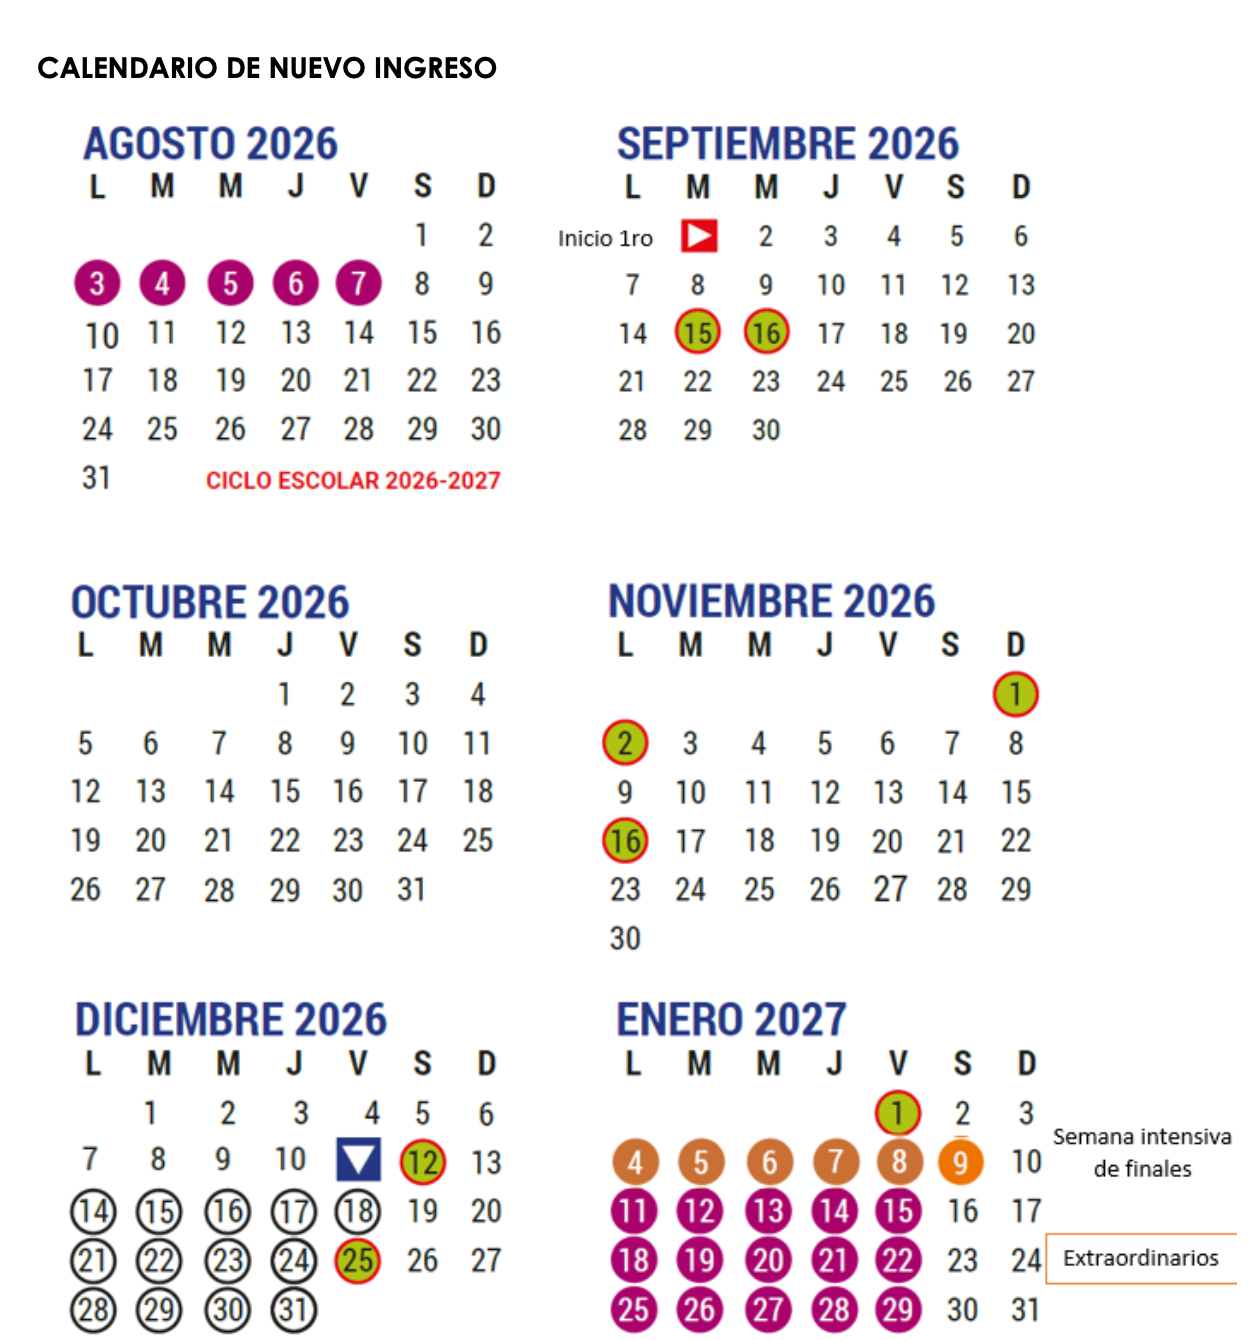
\includegraphics[keepaspectratio]{figures/calendario2027_1.png}}
\end{center}

\subsubsection{SISTEMA DE PUNTOS EXTRAS - TOP 3
KAHOOT}\label{sistema-de-puntos-extras---top-3-kahoot}

\textbf{Estructura:}

\begin{itemize}
\tightlist
\item
  Duración: 10 minutos
\item
  Formato: Preguntas de opción múltiple
\item
  Temas: Conceptos vistos en la semana anterior
\item
  Frecuencia: Cada martes
\end{itemize}

\textbf{Requisitos:}

\begin{itemize}
\tightlist
\item
  Estar en el top 3 (primeros 3 lugares) en Kahoot
\item
  Acumular 10 veces en el top 3 = +1 punto extra
\item
  El punto NO no es transferible (no se pueden pasar a otro estudiante)
\item
  Máximo +1 punto extra por persona
\end{itemize}

\section{References}\label{references-1}

\begin{itemize}
\tightlist
\item
  \href{https://docs.google.com/document/d/17rDksWqGWQqDFUMFqzgVF_BXnBDP3KMUrysgxIPGv9U/edit?usp=sharing}{Plan
  de estudio de la materia}
\end{itemize}

\part{\textbf{Sección 1} - Componentes de una computadora}

\chapter{Introducción a los Componentes de una
Computadora}\label{introducciuxf3n-a-los-componentes-de-una-computadora}

\begin{quote}
\textbf{Fecha:} 01 de septiembre, 2026
\end{quote}

\textbf{Objetivos:}

\begin{enumerate}
\def\labelenumi{\arabic{enumi}.}
\tightlist
\item
  Identificar los componentes internos principales y complementarios
\item
  Diferenciar entre Hardware y Software
\end{enumerate}

\section{\texorpdfstring{\textbf{BLOQUE 1 ---} Hardware vs
Software}{BLOQUE 1 --- Hardware vs Software}}\label{bloque-1-hardware-vs-software}

\begin{figure}[H]

{\centering \pandocbounded{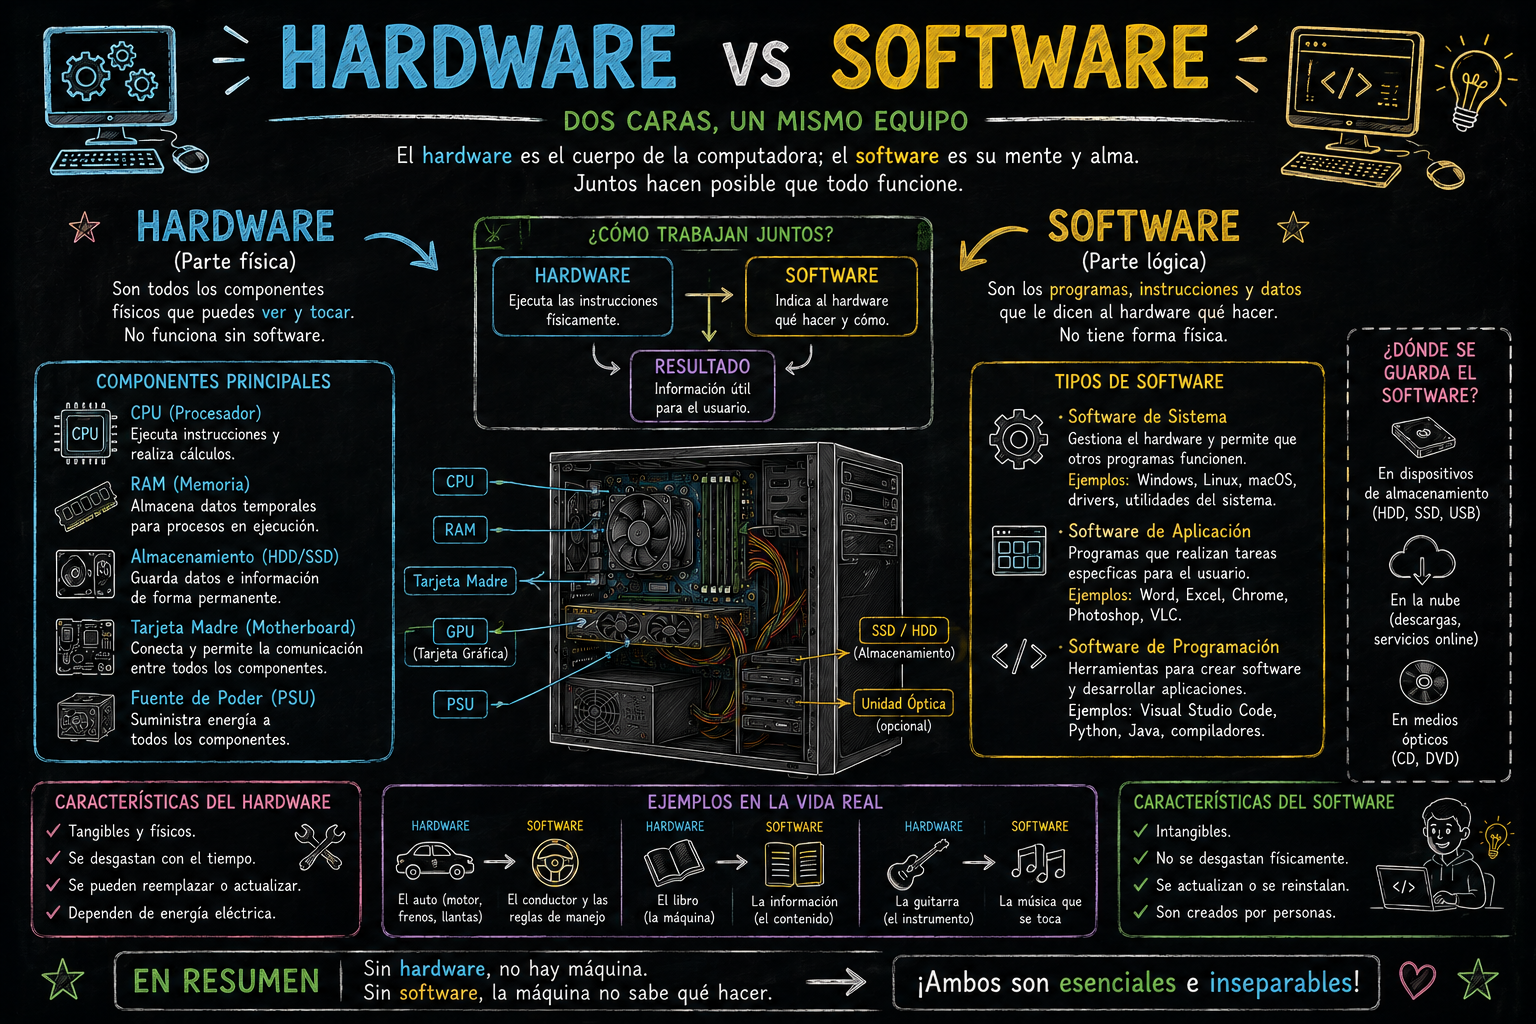
\includegraphics[keepaspectratio]{figures/hardware_vs_software.png}}

}

\caption{Imagen creada con ChatGPT.}

\end{figure}%

Tabla de las diferencias:

{\def\LTcaptype{none} % do not increment counter
\begin{longtable}[]{@{}
  >{\raggedright\arraybackslash}p{(\linewidth - 4\tabcolsep) * \real{0.3333}}
  >{\raggedright\arraybackslash}p{(\linewidth - 4\tabcolsep) * \real{0.3333}}
  >{\raggedright\arraybackslash}p{(\linewidth - 4\tabcolsep) * \real{0.3333}}@{}}
\toprule\noalign{}
\endhead
\bottomrule\noalign{}
\endlastfoot
\textbf{Característica} & \textbf{Hardware} & \textbf{Software} \\
\textbf{Definición} & Componentes físicos y materiales. & Conjunto de
programas, instrucciones y datos. \\
\textbf{Tangibilidad} & Es \textbf{tangible} (se puede tocar, ver y
sostener). & Es \textbf{intangible} (código digital, no se puede
tocar). \\
\textbf{Función} & Ejecutar las tareas físicas y almacenar/procesar
datos electrónicamente. & Dar órdenes al hardware y permitir la
interacción con el usuario. \\
\textbf{Durabilidad / Desgaste} & Se desgasta con el tiempo y el uso
(fallas mecánicas o térmicas). & No se desgasta físicamente, aunque
puede volverse obsoleto o presentar \emph{bugs}. \\
\textbf{Mantenimiento} & Se repara limpiando o reemplazando piezas
físicas. & Se actualiza, se corrigen errores mediante parches o se
reinstala. \\
\textbf{Infección por Virus} & No puede ser infectado directamente por
virus informáticos. & Puede ser infectado por \emph{malware} o virus. \\
\textbf{Ejemplos} & Procesador (CPU), Tarjeta Madre, Monitor, Teclado,
Disco SSD. & Sistema Operativo (Windows, Linux), Navegador Web, Python,
R, Office. \\
\end{longtable}
}

\section{¿Cómo interactúan entre
sí?}\label{cuxf3mo-interactuxfaan-entre-suxed}

El hardware y el software no pueden funcionar de manera independiente:

\begin{enumerate}
\def\labelenumi{\arabic{enumi}.}
\item
  \textbf{El Hardware necesita al Software:} Sin un sistema operativo o
  programas, una computadora es solo una estructura de metal y silicio
  sin capacidad de realizar tareas útiles.
\item
  \textbf{El Software necesita al Hardware:} Las instrucciones del
  código no pueden ejecutarse ni procesarse si no existe un procesador,
  memoria o pantalla donde mostrar los resultados.
\end{enumerate}

\section{\texorpdfstring{\textbf{BLOQUE 2 ---} Componentes Internos
Principales}{BLOQUE 2 --- Componentes Internos Principales}}\label{bloque-2-componentes-internos-principales}

\subsubsection{CPU --- Procesador}\label{cpu-procesador}

\begin{itemize}
\tightlist
\item
  🧠 El ``cerebro'' de la computadora
\item
  Ejecuta instrucciones: \textbf{fetch → decode → execute}
\item
  Características clave:

  \begin{itemize}
  \tightlist
  \item
    Núcleos (cores): más núcleos = más tareas simultáneas
  \item
    Velocidad en \textbf{GigaHertz} (GHz)
  \item
    Memoria Caché (L1, L2, L3)
  \end{itemize}
\item
  Marcas: \textbf{Intel} (Core i3/i5/i7/i9) y \textbf{AMD} (Ryzen)
\item
  Analogía: \emph{``Es como el chef de un restaurante: recibe pedidos,
  los procesa y entrega resultados''} 👨🍳
\end{itemize}

\begin{figure}[H]

{\centering \pandocbounded{
\includegraphics[keepaspectratio]{figures/computadora_CPU.png}}

}

\caption{Imagen creada con ChatGPT.}

\end{figure}%

\begin{tcolorbox}[enhanced jigsaw, arc=.35mm, bottomrule=.15mm, bottomtitle=1mm, breakable, colback=white, colbacktitle=quarto-callout-note-color!10!white, colframe=quarto-callout-note-color-frame, coltitle=black, left=2mm, leftrule=.75mm, opacityback=0, opacitybacktitle=0.6, rightrule=.15mm, title=\textcolor{quarto-callout-note-color}{\faInfo}\hspace{0.5em}{¿Qué es GHz?}, titlerule=0mm, toprule=.15mm, toptitle=1mm]

Es la unidad que mide la \textbf{velocidad del reloj} de un procesador,
es decir, \textbf{cuántas veces por segundo puede ejecutar un ciclo de
instrucciones.}

\begin{verbatim}
1 Hz   = 1 ciclo por segundo 
1 KHz  = 1,000 ciclos por segundo
1 MHz  = 1,000,000 ciclos por segundo
1 GHz  = 1,000,000,000 ciclos por segundo
                  ⬆️
         ¡MIL MILLONES de ciclos por segundo!
\end{verbatim}

Un ciclo es el \textbf{latido del procesador}, marcado por un reloj
interno llamado \textbf{Clock}

\end{tcolorbox}

\subsubsection{RAM --- Memoria de Acceso
Aleatorio}\label{ram-memoria-de-acceso-aleatorio}

\begin{figure}[H]

{\centering 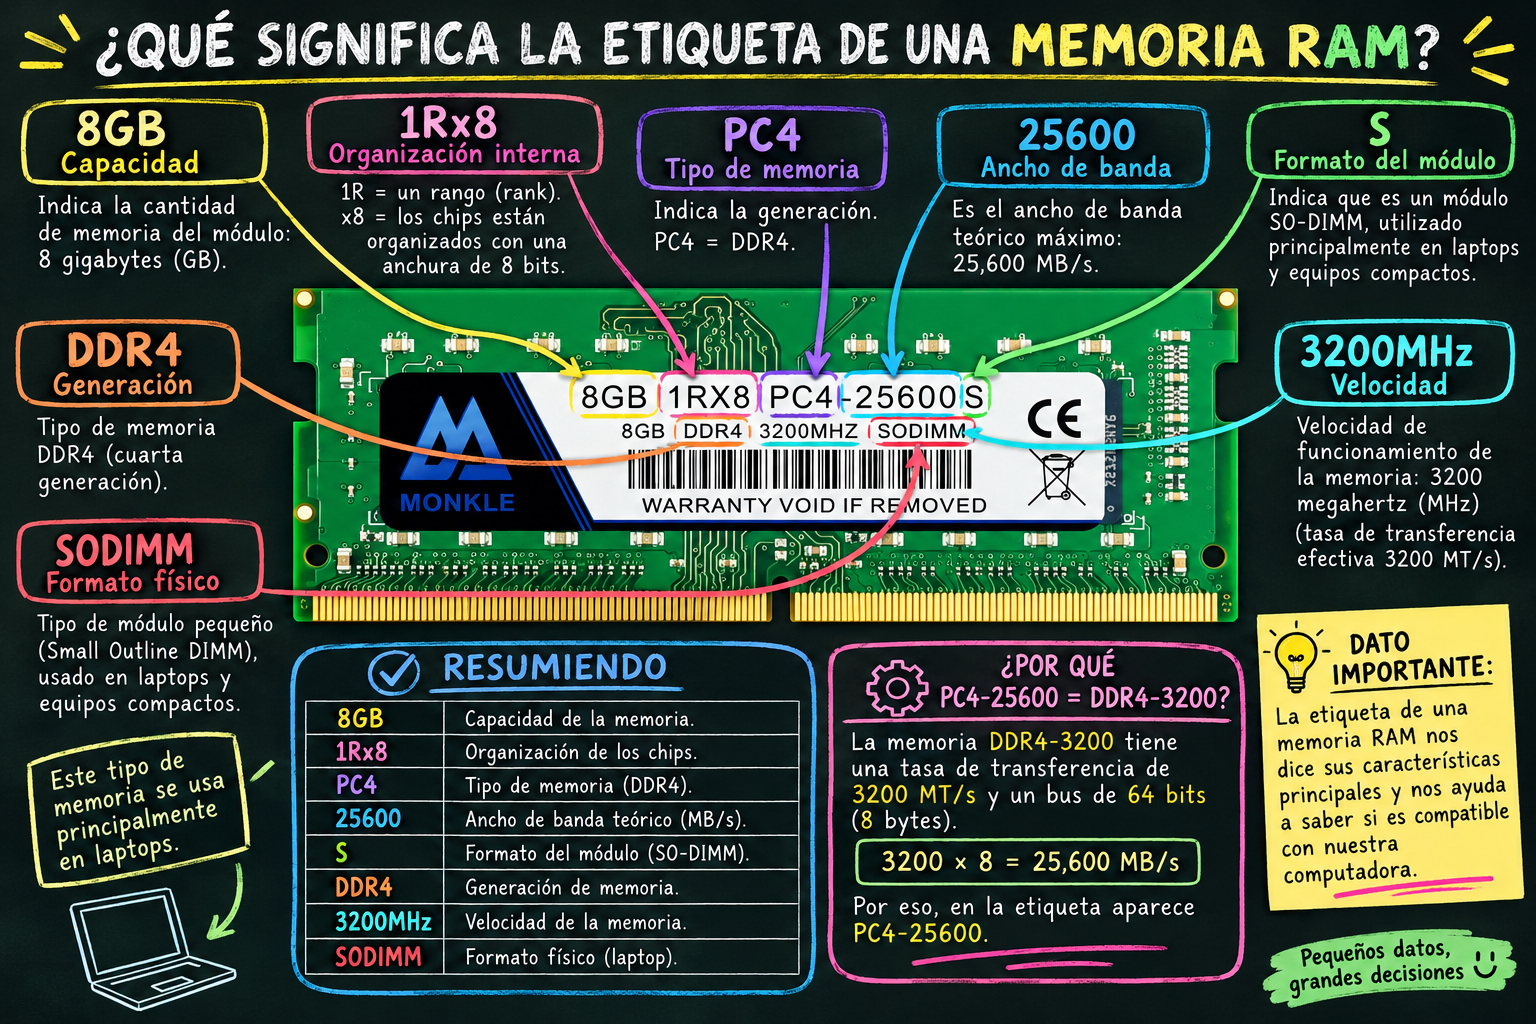
\includegraphics[width=7.13542in,height=\textheight,keepaspectratio]{figures/computadora_ram_v2.png}

}

\caption{Imagen modificada y creada con ChatGPT. Producto real: Memoria
RAM DDR4 8GB 3200MHz SODIMM 260 Pines Monkle para Laptop}

\end{figure}%

\begin{itemize}
\tightlist
\item
  📋 Memoria de trabajo \textbf{temporal}
\item
  Almacena lo que está en uso en este momento
\item
  Se borra al apagar la computadora
\item
  Medida en gigabyte (\textbf{GB)} (8GB, 16GB, 32GB\ldots)
\item
  Tipos: DDR4, DDR5
\item
  Analogía: \emph{``Es el escritorio donde tienes todo lo que estás
  usando ahora''} 🗂️
\end{itemize}

\begin{figure}[H]

{\centering 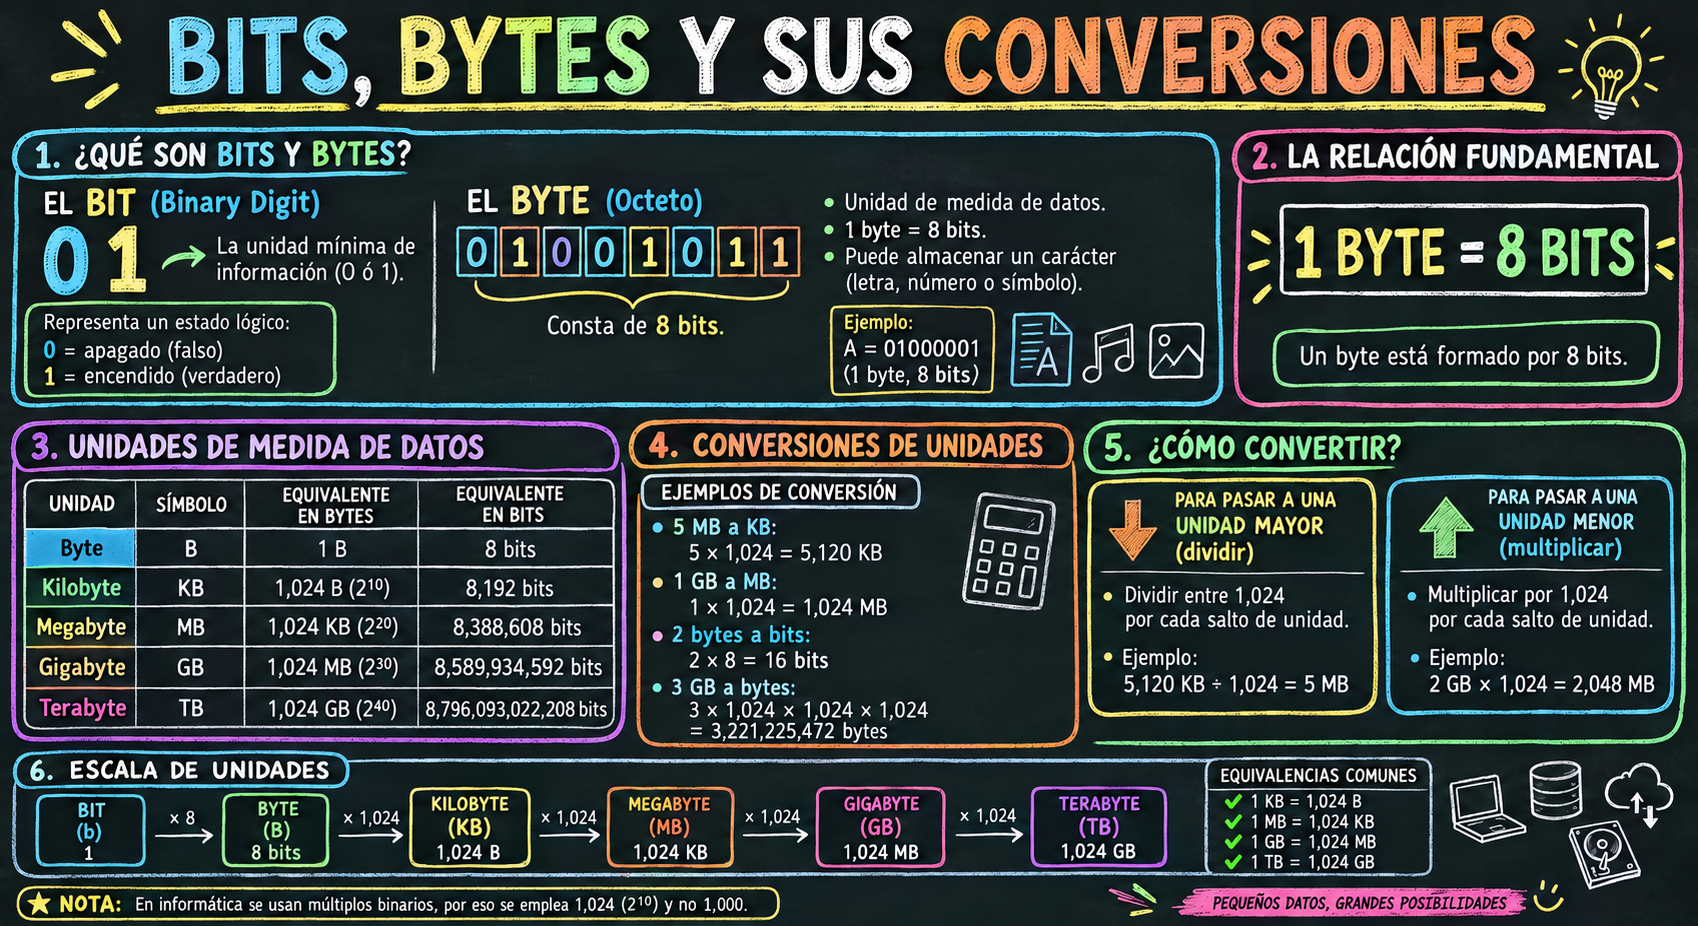
\includegraphics[width=7.25in,height=\textheight,keepaspectratio]{figures/computadora_ram.jpeg}

}

\caption{Imagen generada con Gemini y ChatGPT.}

\end{figure}%

\subsubsection{Almacenamiento --- HDD y
SSD}\label{almacenamiento-hdd-y-ssd}

\begin{figure}[H]

{\centering 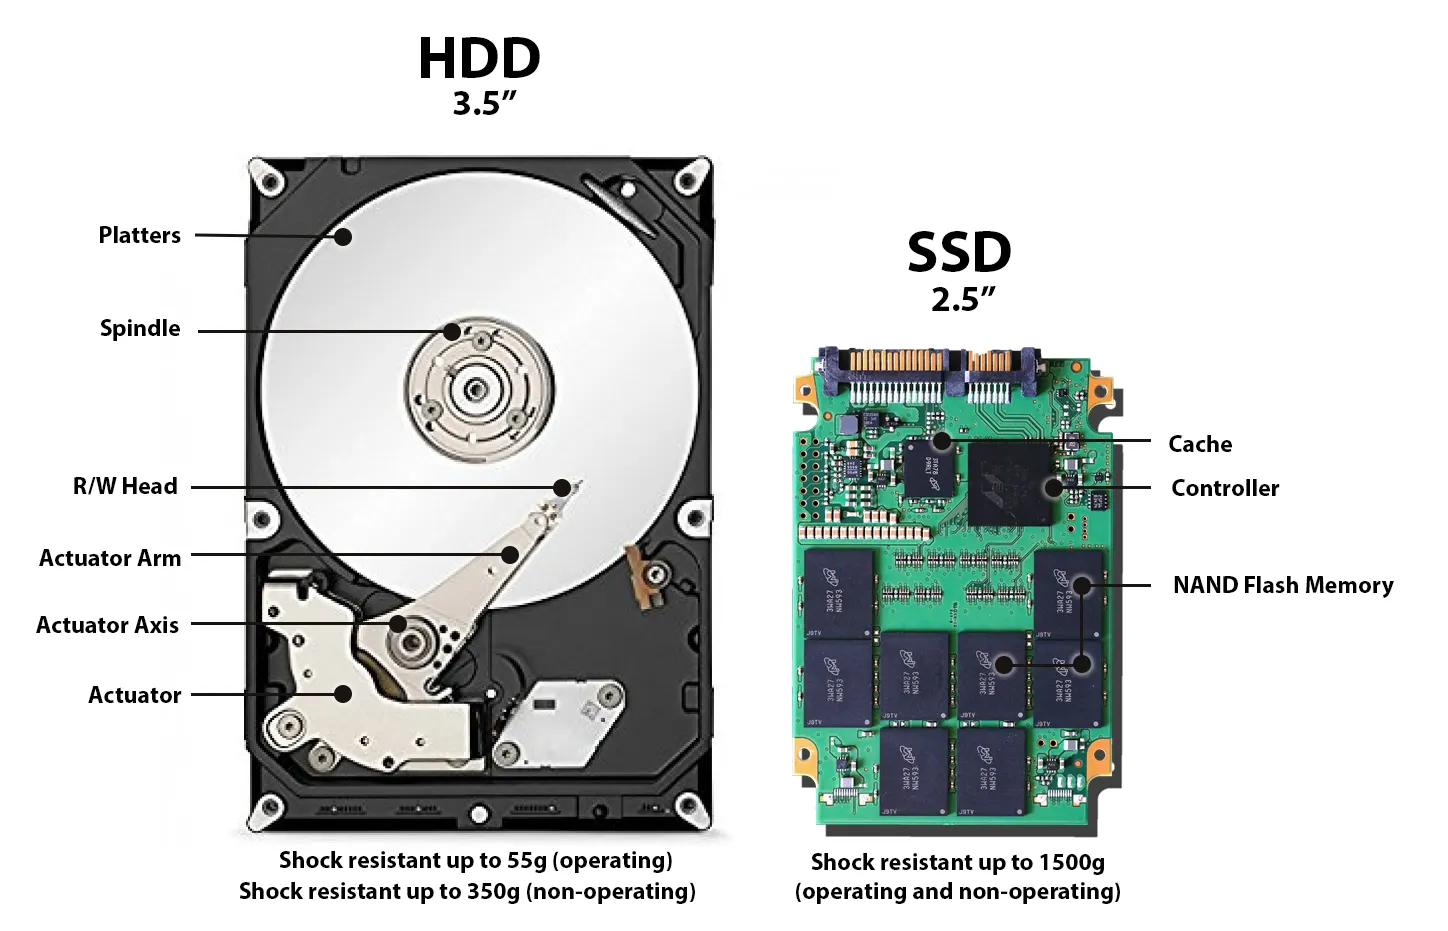
\includegraphics[width=6.11458in,height=\textheight,keepaspectratio]{figures/computadora_discoduro.jpeg}

}

\caption{Comparación entre HDD vs SSD}

\end{figure}%

\begin{quote}
💾 Memoria \textbf{permanente} de la computadora
\end{quote}

\begin{itemize}
\item
  \textbf{HDD} (Disco Duro):

  \begin{itemize}
  \tightlist
  \item
    Mecánico, con platos giratorios
  \item
    Mayor capacidad, menor precio
  \item
    Más lento y frágil
  \end{itemize}
\item
  \textbf{SSD} (Unidad de Estado Sólido):

  \begin{itemize}
  \tightlist
  \item
    Sin partes móviles
  \item
    Mucho más rápido
  \item
    Mayor durabilidad
  \end{itemize}
\item
  Analogía: \emph{``Es el cajón donde guardas todo aunque apagues la
  luz''} 🗄️
\end{itemize}

\begin{figure}[H]

{\centering 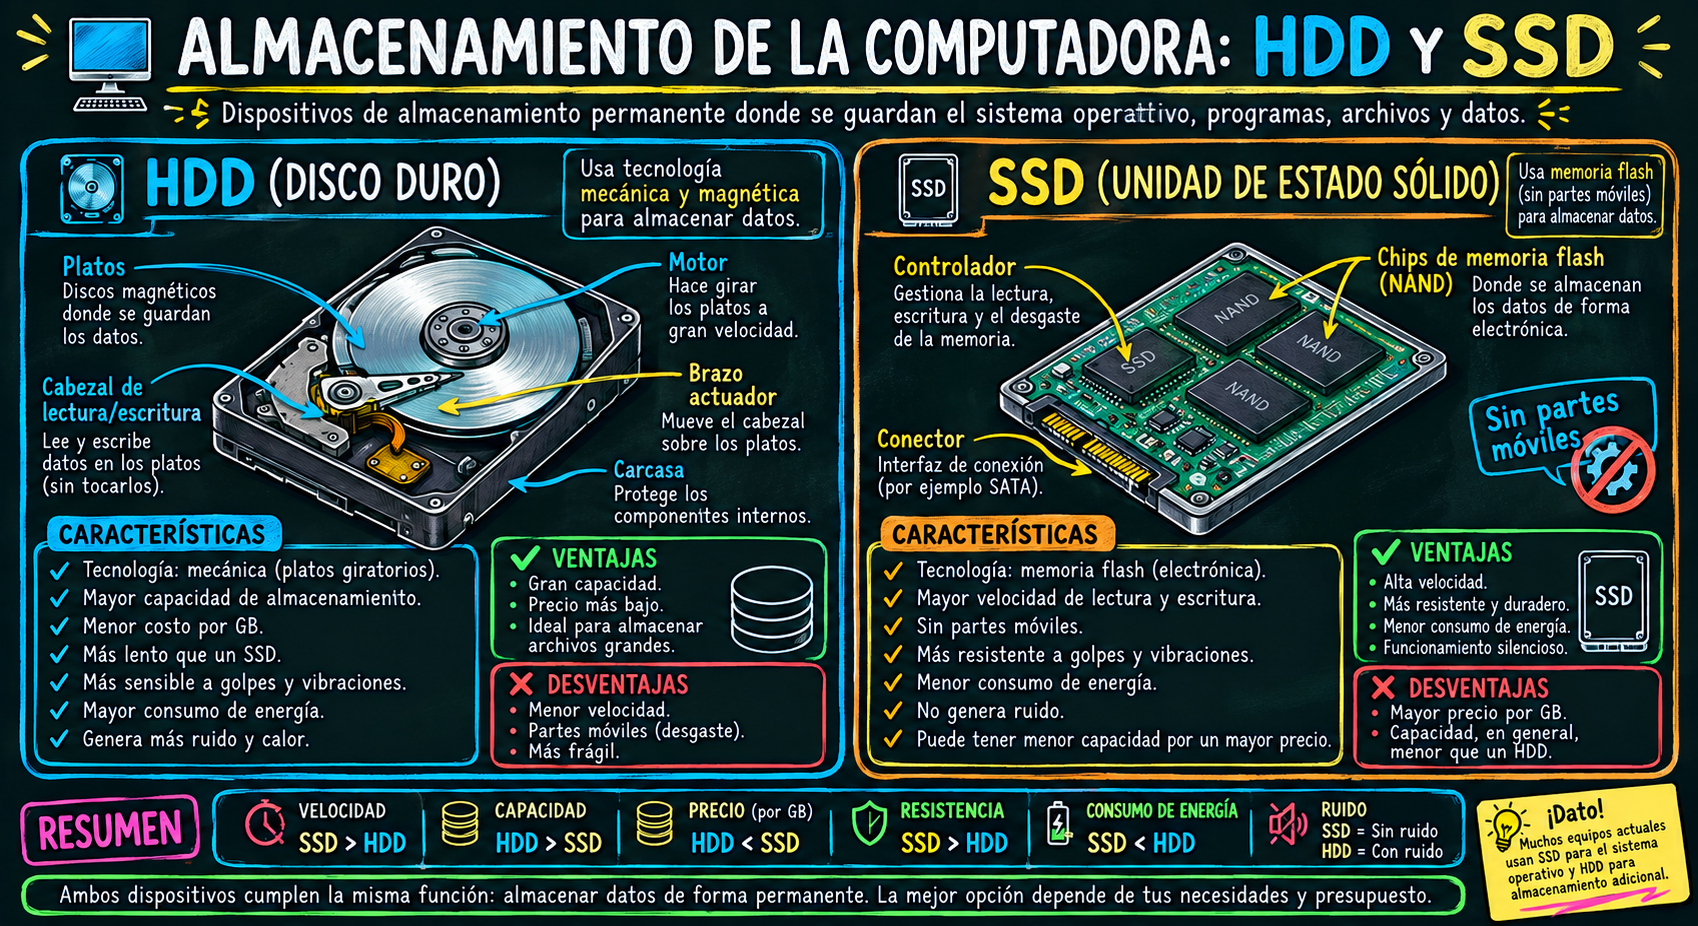
\includegraphics[width=7.27083in,height=\textheight,keepaspectratio]{figures/computadora_memoria.jpeg}

}

\caption{Imagen creada con ChatGPT y Gemini.}

\end{figure}%

\begin{tcolorbox}[enhanced jigsaw, arc=.35mm, bottomrule=.15mm, bottomtitle=1mm, breakable, colback=white, colbacktitle=quarto-callout-note-color!10!white, colframe=quarto-callout-note-color-frame, coltitle=black, left=2mm, leftrule=.75mm, opacityback=0, opacitybacktitle=0.6, rightrule=.15mm, title=\textcolor{quarto-callout-note-color}{\faInfo}\hspace{0.5em}{¿Qué es la Memoria Caché?}, titlerule=0mm, toprule=.15mm, toptitle=1mm]

Es una memoria \textbf{ultrarrápida} y \textbf{pequeña} que vive dentro
del CPU y guarda temporalmente los datos que usa con más frecuencia,
para no tener que ir a buscarlos a la RAM cada vez.

Primero entendamos \textbf{por qué existe}:

\begin{verbatim}
Velocidad de los componentes:

🧠 CPU        →  opera a    4 GHz    (ultrarrápido)
💾 RAM        →  opera a    ~50 GHz  (rápido)
💿 SSD        →  opera a    ~500 MB/s (lento)
📀 HDD        →  opera a    ~100 MB/s (muy lento)

⚠️ El problema:
El CPU es TAN rápido que si tuviera que esperar a que la RAM le diera datos... perdería el 99% de su tiempo ESPERANDO 😴
\end{verbatim}

\begin{quote}
💡 \emph{``La caché existe para que el CPU nunca tenga que esperar''}
\end{quote}

\subsection{\texorpdfstring{\textbf{Analogía}}{Analogía}}\label{analoguxeda}

\begin{figure}[H]

{\centering \pandocbounded{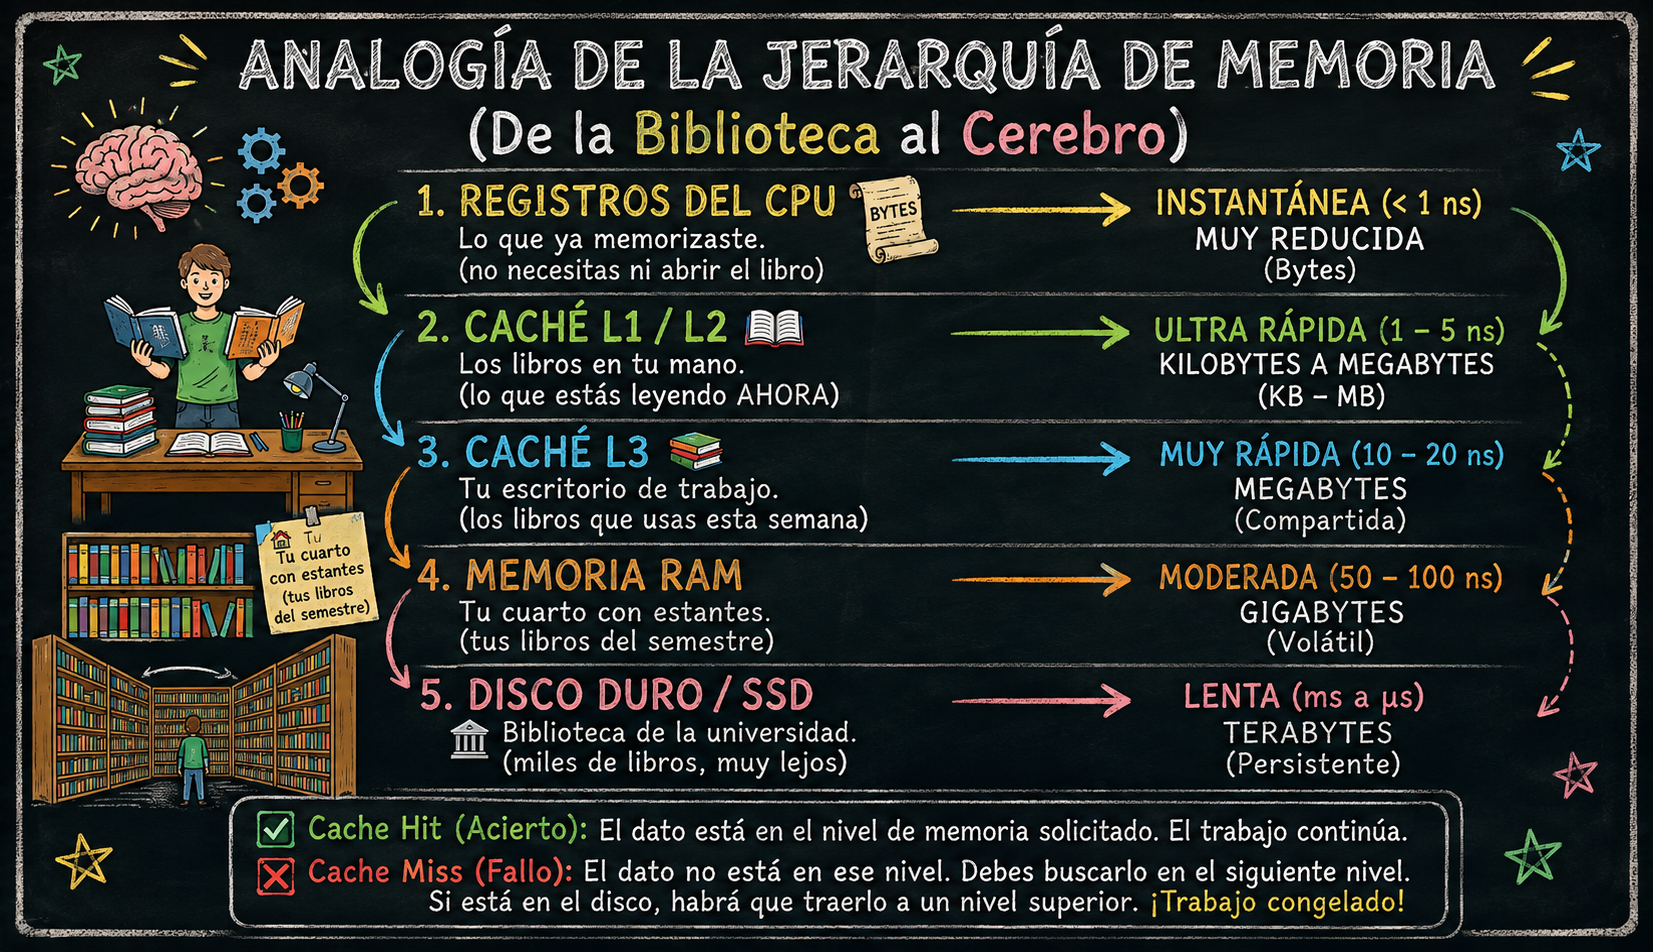
\includegraphics[keepaspectratio]{figures/computadora_cache.jpeg}}

}

\caption{Imagen creada con ChatGPT, Gemini y uDocz.}

\end{figure}%

Escala de tiempo:

\begin{verbatim}
1 segundo    =  1 s
1 milisegundo = 0.001 s        (ms) → parpadeo de un ojo
1 microsegundo = 0.000001 s    (µs) → cámara de alta velocidad
1 nanosegundo = 0.000000001 s  (ns) → velocidad del CPU ⚡
\end{verbatim}

\begin{quote}
🔑 \emph{``Mientras más cerca está la información del CPU, más rápido
puede trabajar''}
\end{quote}

\end{tcolorbox}

\subsubsection{Tarjeta Madre ---
Motherboard}\label{tarjeta-madre-motherboard}

\begin{itemize}
\tightlist
\item
  🔌 El ``esqueleto'' que conecta todo
\item
  Contiene los \textbf{buses de datos} que comunican componentes
\item
  Incluye: slots para RAM, CPU, GPU, almacenamiento
\item
  Tiene el \textbf{BIOS/UEFI}: primer software que corre al encender
\item
  Fabricantes: ASUS, MSI, Gigabyte
\end{itemize}

\begin{figure}[H]

{\centering \pandocbounded{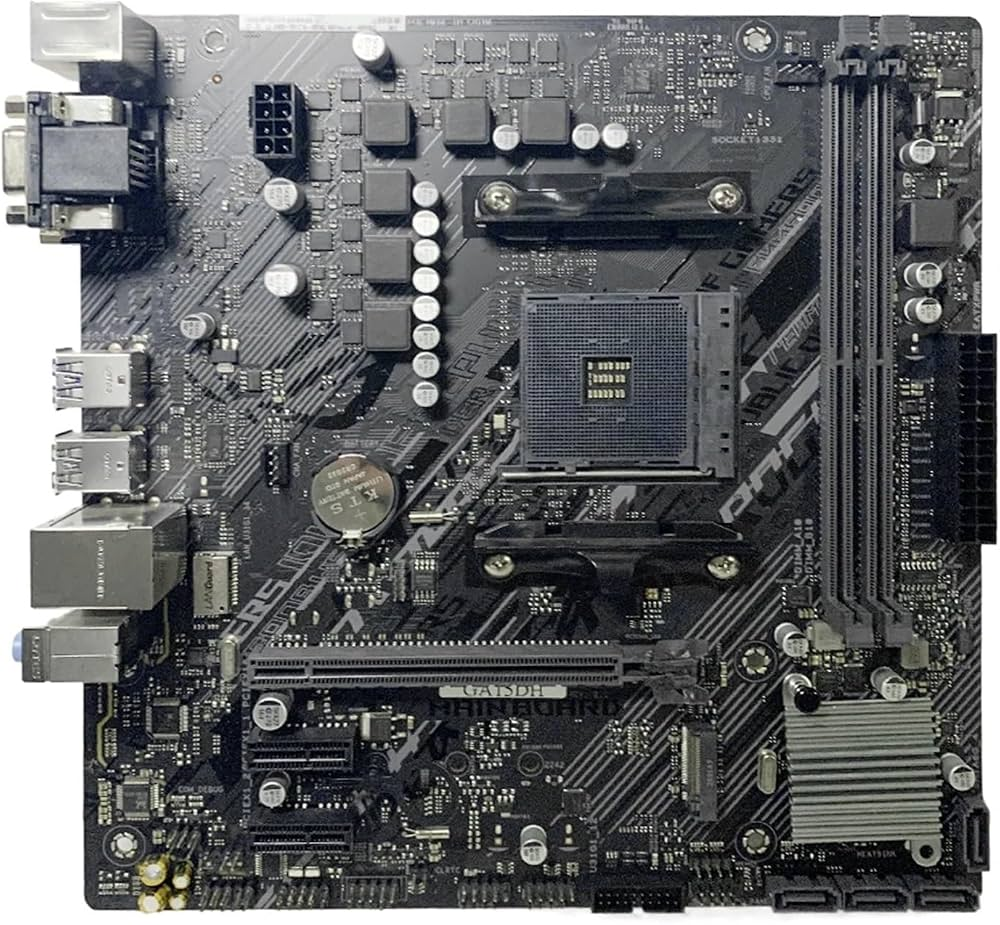
\includegraphics[keepaspectratio]{figures/PlacaMadreSUS_B450_GA15DH .jpg}}

}

\caption{Placa Madre Gaming creada por ASUS, contiene el chip B450,
modelo GA15DH con procesador Ryzen 7 1700 3700x.}

\end{figure}%

\subsubsection{GPU (Graphics Processing Unit) - unidad de procesamiento
gráfico}\label{gpu-graphics-processing-unit---unidad-de-procesamiento-gruxe1fico}

\begin{itemize}
\item
  Es el CHIP procesador gráfico; Solo el cerebro, el procesador en sí.

  \begin{itemize}
  \tightlist
  \item
    Ejemplo: el chip ``AD102'' de NVIDIA → RTX 4090.
  \end{itemize}
\end{itemize}

\subsubsection{Tarjeta Gráfica}\label{tarjeta-gruxe1fica}

\begin{itemize}
\tightlist
\item
  Es el PRODUCTO COMPLETO:

  \begin{itemize}
  \tightlist
  \item
    GPU (chip procesador)
  \item
    PCB (Placa de Circuito Impreso): es donde van soldados todos los
    componentes
  \item
    GRAM (Graphics Random Access Memory): módulos de memoria, también
    conocida como VRAM (Video RAM) → texturas
  \item
    🔵 Condensadores: Estabilizan y filtran la energía eléctrica
  \item
    🟡 Inductores: Regulan el voltaje que llega al GPU
  \item
    🔴 MOSFETs: Controlan el flujo de corriente
  \item
    ⚫ Resistencias: Limitan y controlan la corriente
  \item
    🟢 VRM (Voltage Regulator Module): Convierte y regula el voltaje
    para el GPU
  \item
    Tuberías de calor: Son tubos de cobre huecos rellenos de líquido
    especial
  \item
    Ventiladores (o blower)
  \item
    Carcasa
  \end{itemize}
\item
  🎮 Procesa imágenes, video y gráficos 3D
\item
  Tiene su propio procesador (miles de núcleos pequeños)
\item
  Puede ser:

  \begin{itemize}
  \tightlist
  \item
    \textbf{Integrada}: dentro del CPU (uso básico)
  \item
    \textbf{Dedicada}: tarjeta independiente (gaming, diseño, IA)
  \end{itemize}
\item
  Marcas: NVIDIA (GeForce), AMD (Radeon)
\item
  Hoy en día: clave para \textbf{Machine Learning e IA} 🤖
\end{itemize}

\begin{figure}[H]

{\centering \pandocbounded{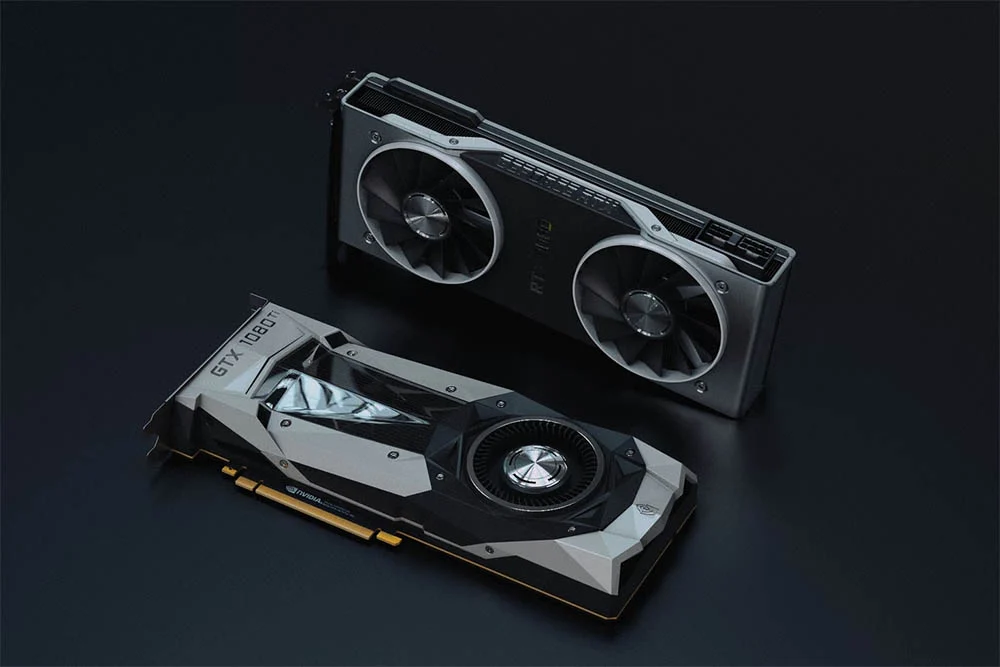
\includegraphics[keepaspectratio]{figures/computadora_tarjetaGrafica.png}}

}

\caption{Ejemplo de una tarjeta Gráfica.}

\end{figure}%

\subsubsection{Fuente de Poder --- PSU}\label{fuente-de-poder-psu}

\begin{itemize}
\tightlist
\item
  ⚡ Convierte la corriente alterna (CA) en corriente directa (CD)
\item
  Alimenta todos los componentes
\item
  Se mide en \textbf{Watts} (500W, 750W, 1000W\ldots)
\item
  Certificaciones de eficiencia: 80 Plus Bronze/Gold/Platinum
\item
  Un componente subestimado pero \textbf{crítico} para la estabilidad
\end{itemize}

\section{\texorpdfstring{\textbf{BLOQUE 3 ---} Componentes
Complementarios (Periféricos y
Accesorios)}{BLOQUE 3 --- Componentes Complementarios (Periféricos y Accesorios)}}\label{bloque-3-componentes-complementarios-perifuxe9ricos-y-accesorios}

Son aquellos dispositivos que se conectan a la computadora para
interactuar con ella, introducir o recibir datos, o mejorar sus
funciones, pero que no impiden que el sistema interno funcione.

\subsection{Periféricos de Entrada}\label{perifuxe9ricos-de-entrada}

Permiten al usuario enviar datos o instrucciones a la computadora:

\begin{itemize}
\tightlist
\item
  \textbf{Teclado y Ratón (Mouse):} Los medios principales para
  interactuar con el sistema.
\item
  \textbf{Micrófono y Cámara Web:} Para videollamadas, grabación de
  audio y conferencias.
\item
  \textbf{Escáner / Lectores de códigos:} Para digitalizar documentos
  físicos.
\end{itemize}

\subsection{Periféricos de Salida}\label{perifuxe9ricos-de-salida}

Muestran o entregan los resultados procesados por la computadora:

\begin{itemize}
\tightlist
\item
  \textbf{Monitor / Pantalla:} Muestra la interfaz gráfica y la
  información visual (\emph{esencial para la interacción humana, aunque
  técnicamente el equipo puede encender sin él}).
\item
  \textbf{Bocinas o Audífonos:} Para la reproducción de audio.
\item
  \textbf{Impresora:} Para trasladar información digital a formato
  físico.
\end{itemize}

\subsection{C. Complementos Internos y Unidades de
Expansión}\label{c.-complementos-internos-y-unidades-de-expansiuxf3n}

\begin{itemize}
\tightlist
\item
  \textbf{Sistemas de Enfriamiento Extra (Líquido o Ventiladores
  adicionales):} Mantienen las temperaturas óptimas en equipos de alto
  rendimiento.
\item
  \textbf{Tarjetas de Red / Wi-Fi o Bluetooth:} Añaden o mejoran la
  conectividad inalámbrica.
\item
  \textbf{Lectores de discos (CD/DVD/Blu-ray):} Cada vez menos comunes,
  útiles para leer formatos físicos antiguos.
\end{itemize}

\begin{figure}[H]

{\centering 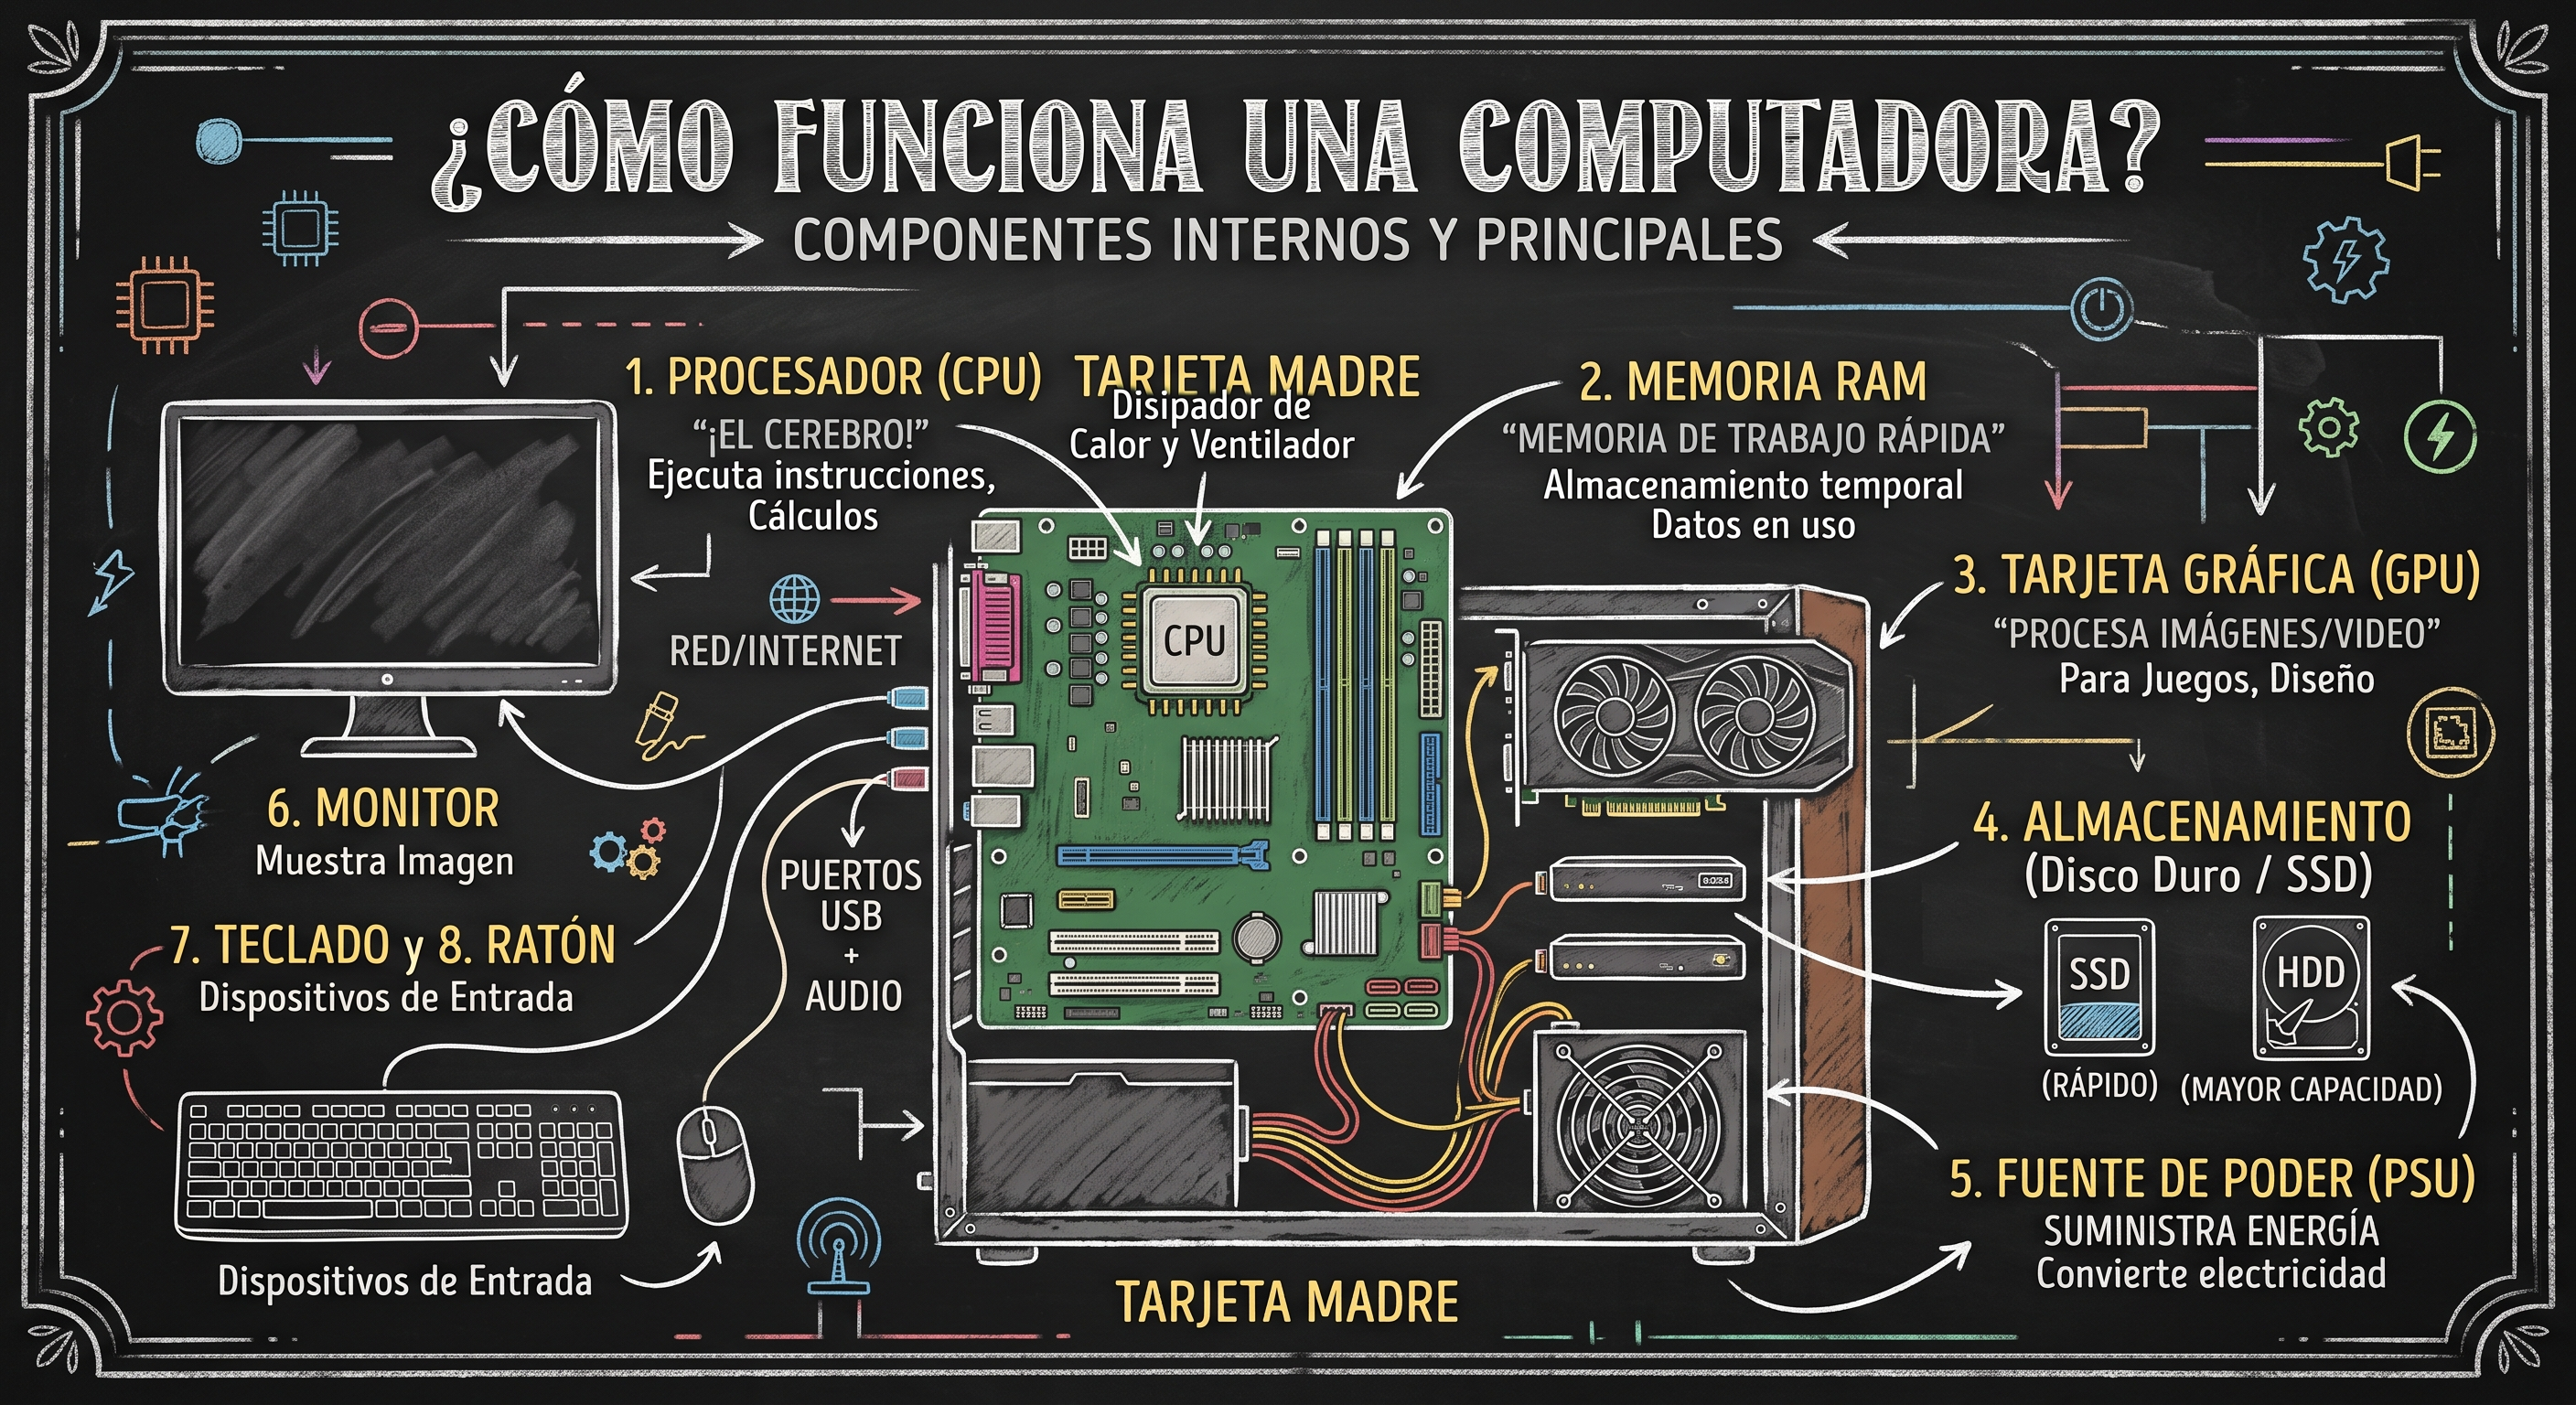
\includegraphics[width=7.5625in,height=\textheight,keepaspectratio]{figures/computadora_componentes.jpeg}

}

\caption{Imagen generada con ChatGPT y Gemini.}

\end{figure}%

\section{\texorpdfstring{\textbf{BLOQUE 4 ---
Firmware}}{BLOQUE 4 --- Firmware}}\label{bloque-4-firmware}

Es un software permanente grabado dentro de un chip de hardware que
controla cómo funciona ese dispositivo.

\subsection{¿Qué es el BIOS?}\label{quuxe9-es-el-bios}

\textbf{BIOS = Basic Input Output System} \textbf{Sistema Básico de
Entrada y Salida}

\begin{quote}
\emph{``Es el primer programa que se ejecuta cuando enciendes tu
computadora, ANTES que cualquier sistema operativo''}
\end{quote}

\subsubsection{¿Dónde vive el BIOS?}\label{duxf3nde-vive-el-bios}

\begin{itemize}
\tightlist
\item
  No está en el disco duro
\item
  No está en la RAM
\item
  No está en el CPU
\item
  Vive en un chip especial de la Tarjeta Madre llamado \textbf{ROM (Read
  Only Memory)}
\end{itemize}

\begin{quote}
``Al estar en \textbf{ROM}, el BIOS no se borra aunque apagues la
computadora''
\end{quote}

Su trabajo principal es \textbf{POST}:

\begin{verbatim}
Power On Self Test  = Prueba de Autodiagnóstico al Encender
\end{verbatim}

\begin{figure}[H]

{\centering \pandocbounded{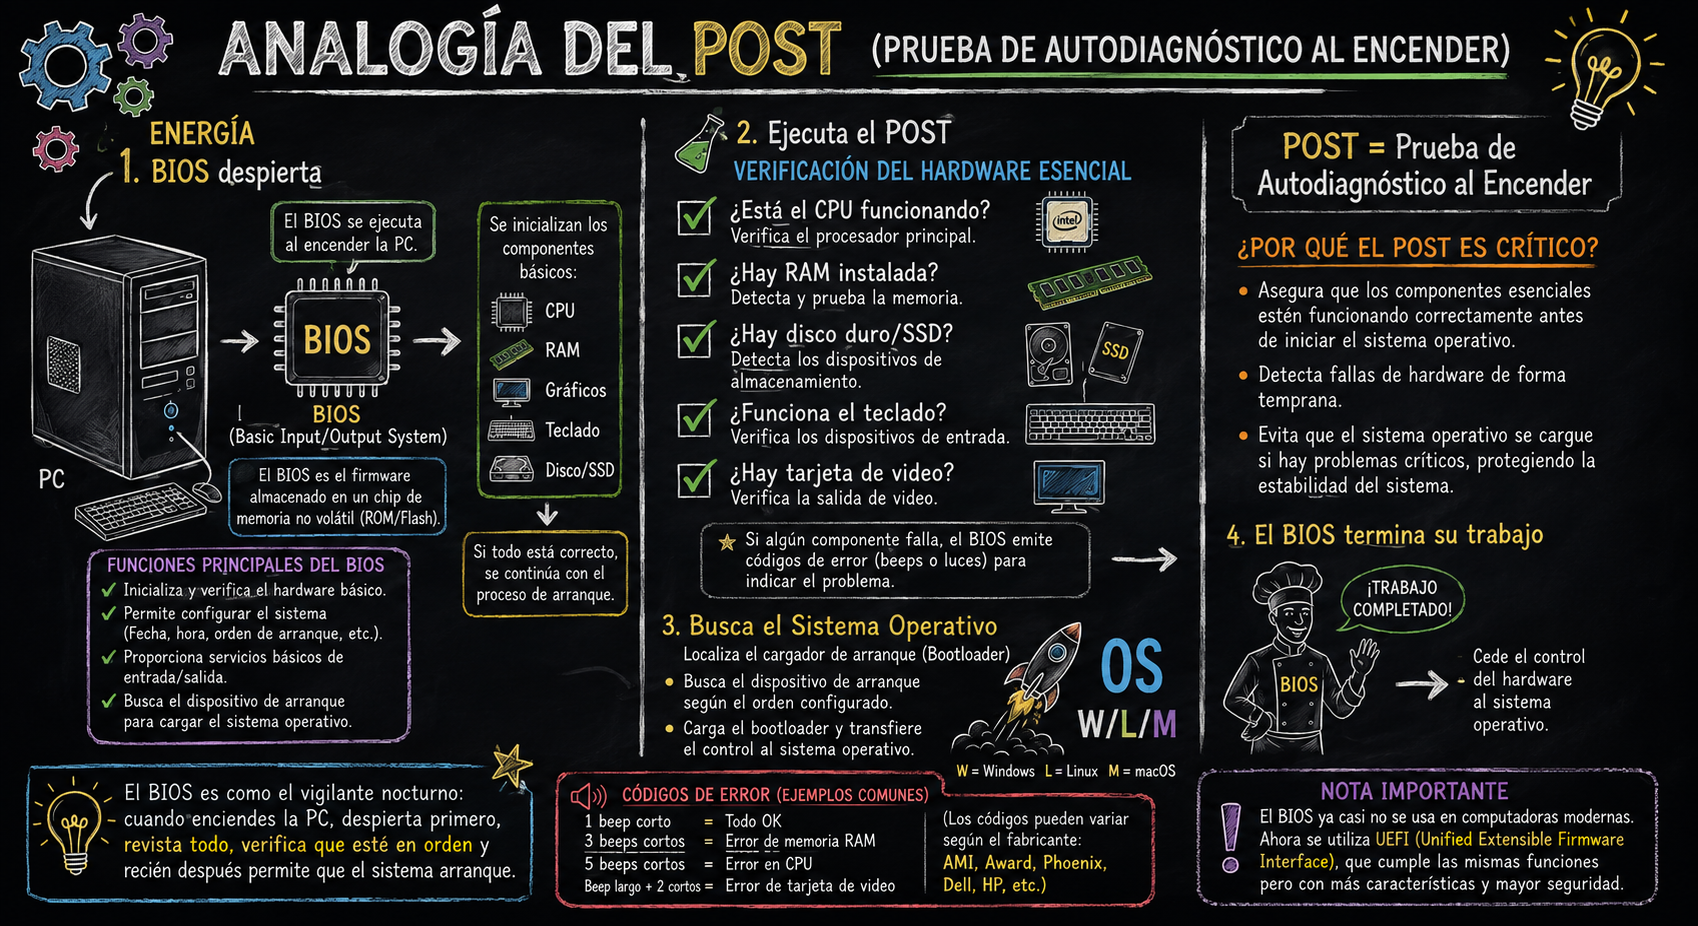
\includegraphics[keepaspectratio]{figures/computadora_bios.jpeg}}

}

\caption{Imagen generada con ChatGPT, Gemini y uDocz. W/L/M: signfiica
Windows, Linux, MacOS; OS: Operating System (Sistema Operativo).}

\end{figure}%

\subsection{¿Sabías que la Motherboard tiene una pequeña
batería?}\label{sabuxedas-que-la-motherboard-tiene-una-pequeuxf1a-bateruxeda}

Esta batería mantiene:

\begin{itemize}
\tightlist
\item
  ⏰ La fecha y hora
\item
  ⚙️ La configuración del BIOS
\item
  🔌 Los ajustes guardados
\end{itemize}

Si se agota → la computadora pierde la hora y configuración cada vez que
se apaga 😱.

\begin{figure}[H]

{\centering \pandocbounded{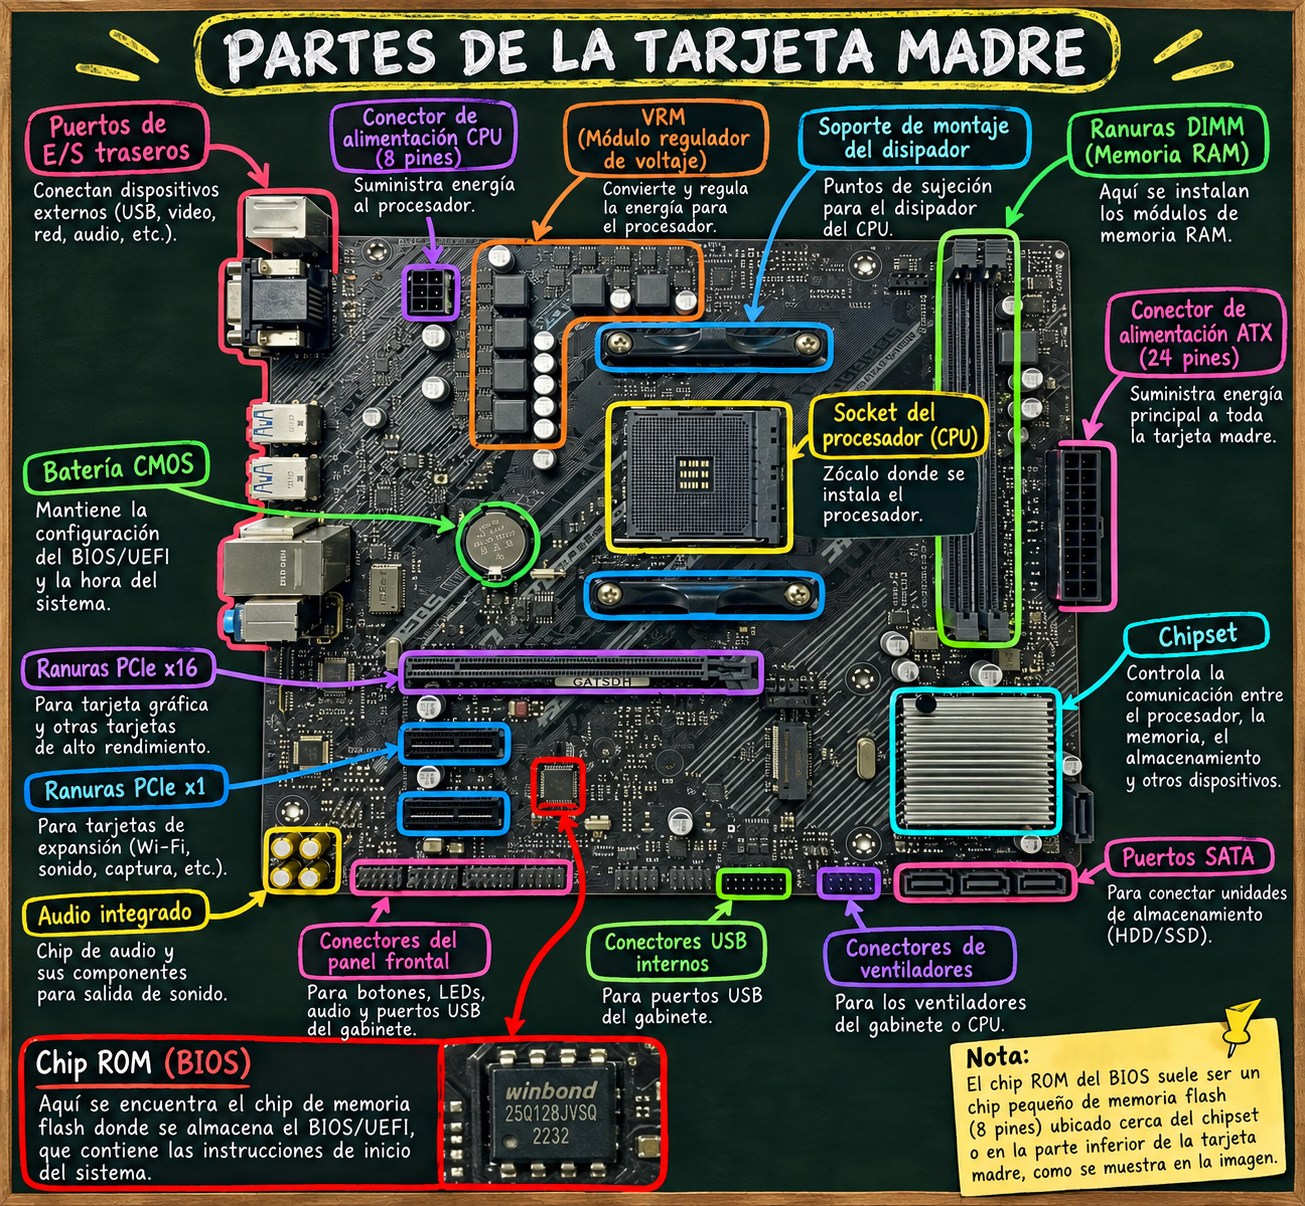
\includegraphics[keepaspectratio]{figures/PlacaMadreSUS_B450_GA15DH_chatgpt.png}}

}

\caption{Misma imagen que arriba pero con clasificación de componentes
realizada por ChatGPT.}

\end{figure}%

\begin{tcolorbox}[enhanced jigsaw, arc=.35mm, bottomrule=.15mm, bottomtitle=1mm, breakable, colback=white, colbacktitle=quarto-callout-important-color!10!white, colframe=quarto-callout-important-color-frame, coltitle=black, left=2mm, leftrule=.75mm, opacityback=0, opacitybacktitle=0.6, rightrule=.15mm, title=\textcolor{quarto-callout-important-color}{\faExclamation}\hspace{0.5em}{BIOS (antes) vs UEFI (ahora)}, titlerule=0mm, toprule=.15mm, toptitle=1mm]

\emph{``El BIOS clásico fue reemplazado por UEFI en computadoras
modernas''}

{\def\LTcaptype{none} % do not increment counter
\begin{longtable}[]{@{}lll@{}}
\toprule\noalign{}
Característica & BIOS (antiguo) & UEFI (moderno) \\
\midrule\noalign{}
\endhead
\bottomrule\noalign{}
\endlastfoot
📅 Año & 1975 & 2005 - presente \\
🖥️ Interfaz & Solo texto & Gráfica con mouse \\
💾 Disco máximo & 2 TB & 9 ZB (sin límite práctico) \\
⚡ Velocidad arranque & Lento & Muy rápido \\
🔐 Seguridad & Básica & Secure Boot \\
🖱️ Mouse & ❌ No & ✅ Sí \\
\end{longtable}
}

\begin{figure}[H]

{\centering \pandocbounded{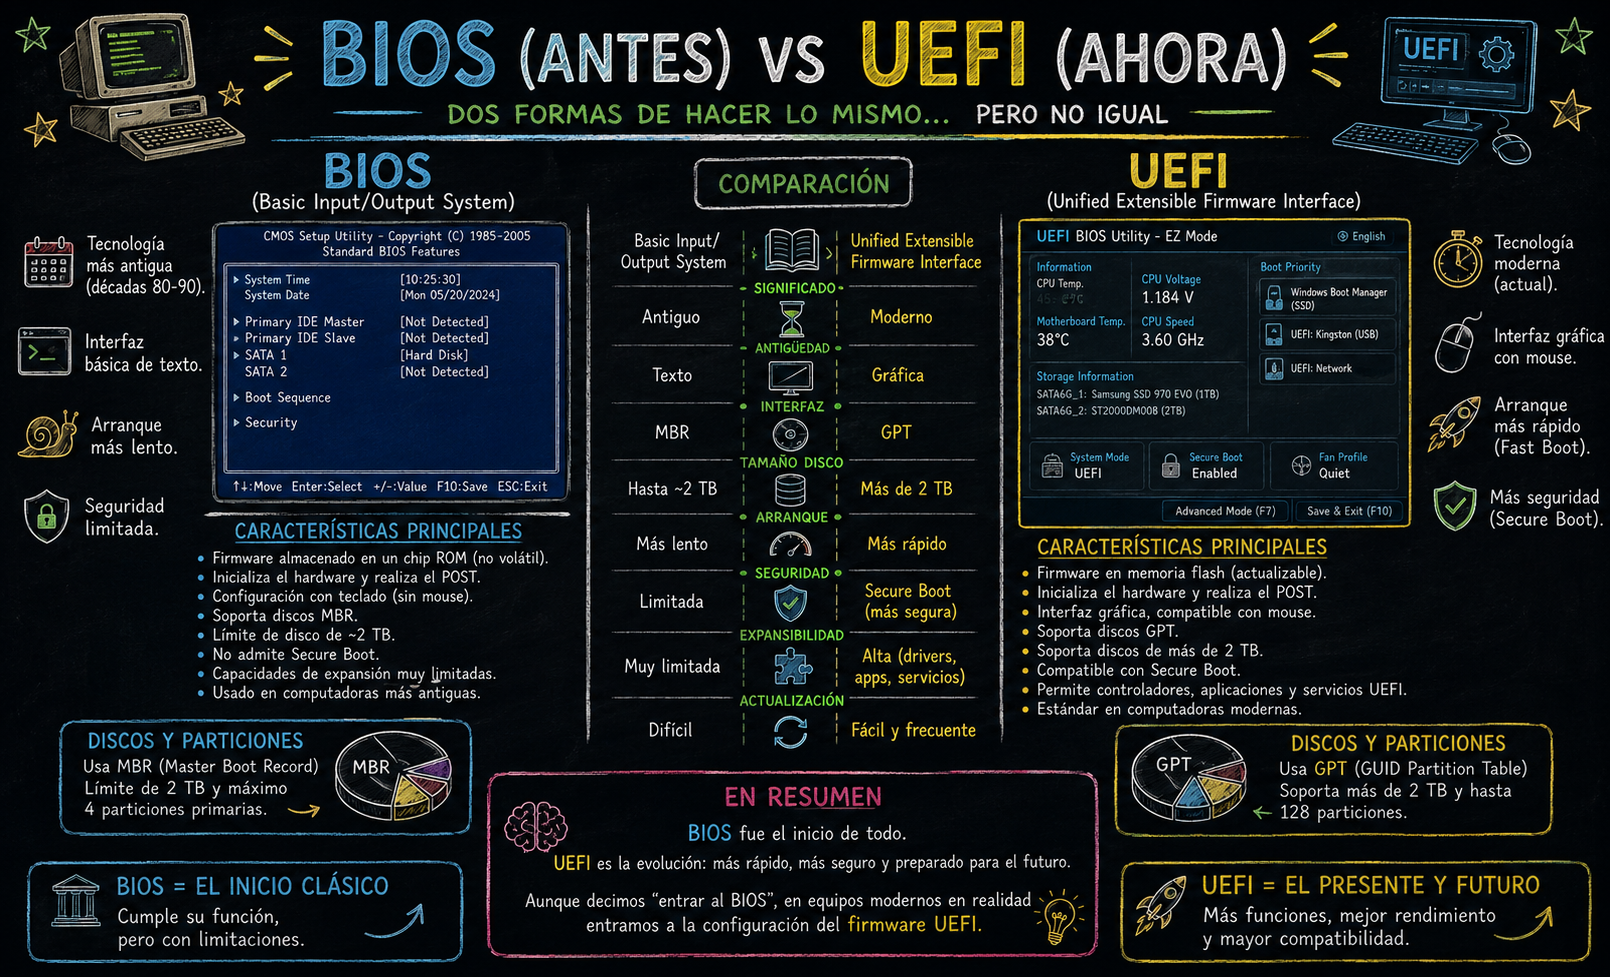
\includegraphics[keepaspectratio]{figures/computadora_uefi.jpeg}}

}

\caption{Imagen generada con ChatGPT, Gemini y uDocz.}

\end{figure}%

\end{tcolorbox}

En resumen \ldots{}

\begin{figure}[H]

{\centering \pandocbounded{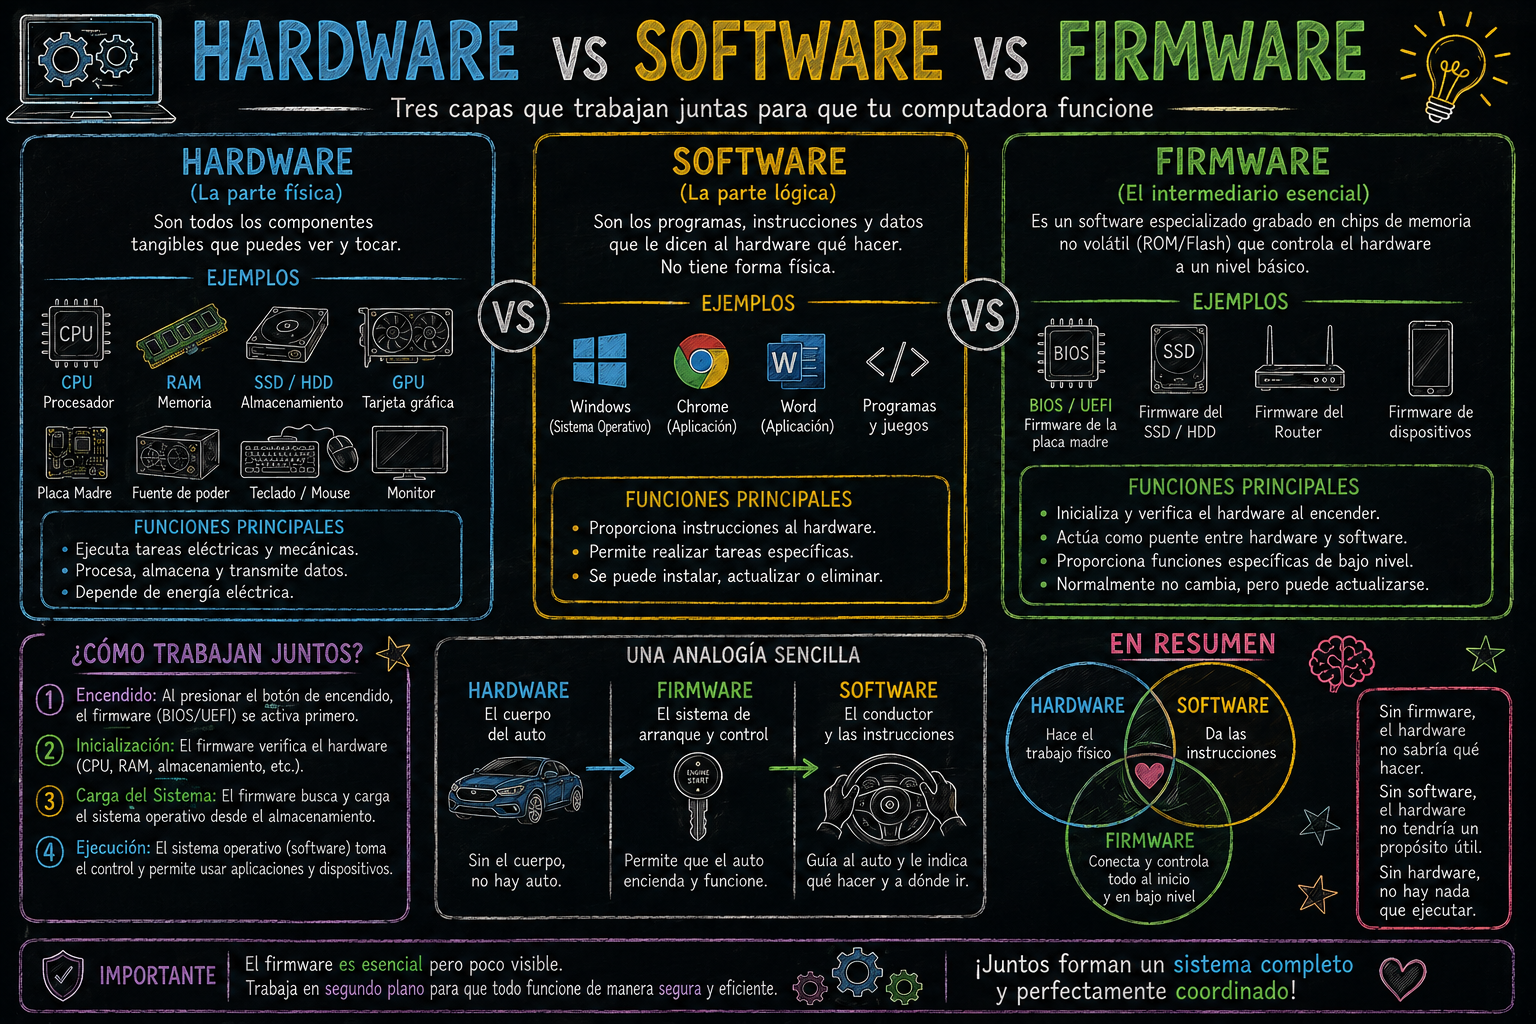
\includegraphics[keepaspectratio]{figures/computadora_resumen.png}}

}

\caption{Imagen creada con ChatGPT.}

\end{figure}%

\section{Referencias}\label{referencias-1}

\begin{itemize}
\tightlist
\item
  \href{https://www.pccomponentes.com/blog/como-elegir-tarjeta-grafica?srsltid=AfmBOooy3DQiJl1fueUUfqybAm1SY6TBkFWnRC-NQuIANQk9eJpnHqez}{¿Qué
  es una tarjeta gráfica? Características y tipos}
\item
  \href{https://medium.com/@rodbauer/hdd-vs-ssd-what-does-the-future-for-storage-hold-dc8653f16366}{HDD
  vs SSD: What Does the Future for Storage Hold?}
\end{itemize}

\chapter{\texorpdfstring{\textbf{🎮 AhaSlides -Manos a la
obra}}{🎮 AhaSlides -Manos a la obra}}\label{ahaslides--manos-a-la-obra}

\begin{tcolorbox}[enhanced jigsaw, arc=.35mm, bottomrule=.15mm, bottomtitle=1mm, breakable, colback=white, colbacktitle=quarto-callout-tip-color!10!white, colframe=quarto-callout-tip-color-frame, coltitle=black, left=2mm, leftrule=.75mm, opacityback=0, opacitybacktitle=0.6, rightrule=.15mm, title=\textcolor{quarto-callout-tip-color}{\faLightbulb}\hspace{0.5em}{AhaSlides Actividad}, titlerule=0mm, toprule=.15mm, toptitle=1mm]

Pon a prueba lo que has aprendido y acumula tus victorias para alcanzar
el punto final. Además, si logras quedar entre los tres primeros lugares
en 10 ocasiones, obtendrás un punto extra como recompensa:

🎮 Unirse como jugador

Ver la dinámica en AhaSlides

👩 Editar sesión (Profesora)

\end{tcolorbox}

\chapter{Sistema Operativo (SO) y sus
funciones}\label{sistema-operativo-so-y-sus-funciones}

\begin{quote}
\textbf{Fecha:} 03 de septiembre, 2026
\end{quote}

\textbf{Objetivos:}

\begin{enumerate}
\def\labelenumi{\arabic{enumi}.}
\tightlist
\item
  Comprender qué es un Sistema Operativo (SO) y cuál es su función
  principal en una computadora
\item
  Identificar los SO más comunes en el mercado actual
\end{enumerate}

\section{¿Qué es un Sistema Operativo (SO) / Operating System
(OS)?}\label{quuxe9-es-un-sistema-operativo-so-operating-system-os}

Es el software principal que actúa como intermediario entre el usuario,
las aplicaciones y el hardware de la computadora o del teléfono.

\begin{figure}[H]

{\centering \pandocbounded{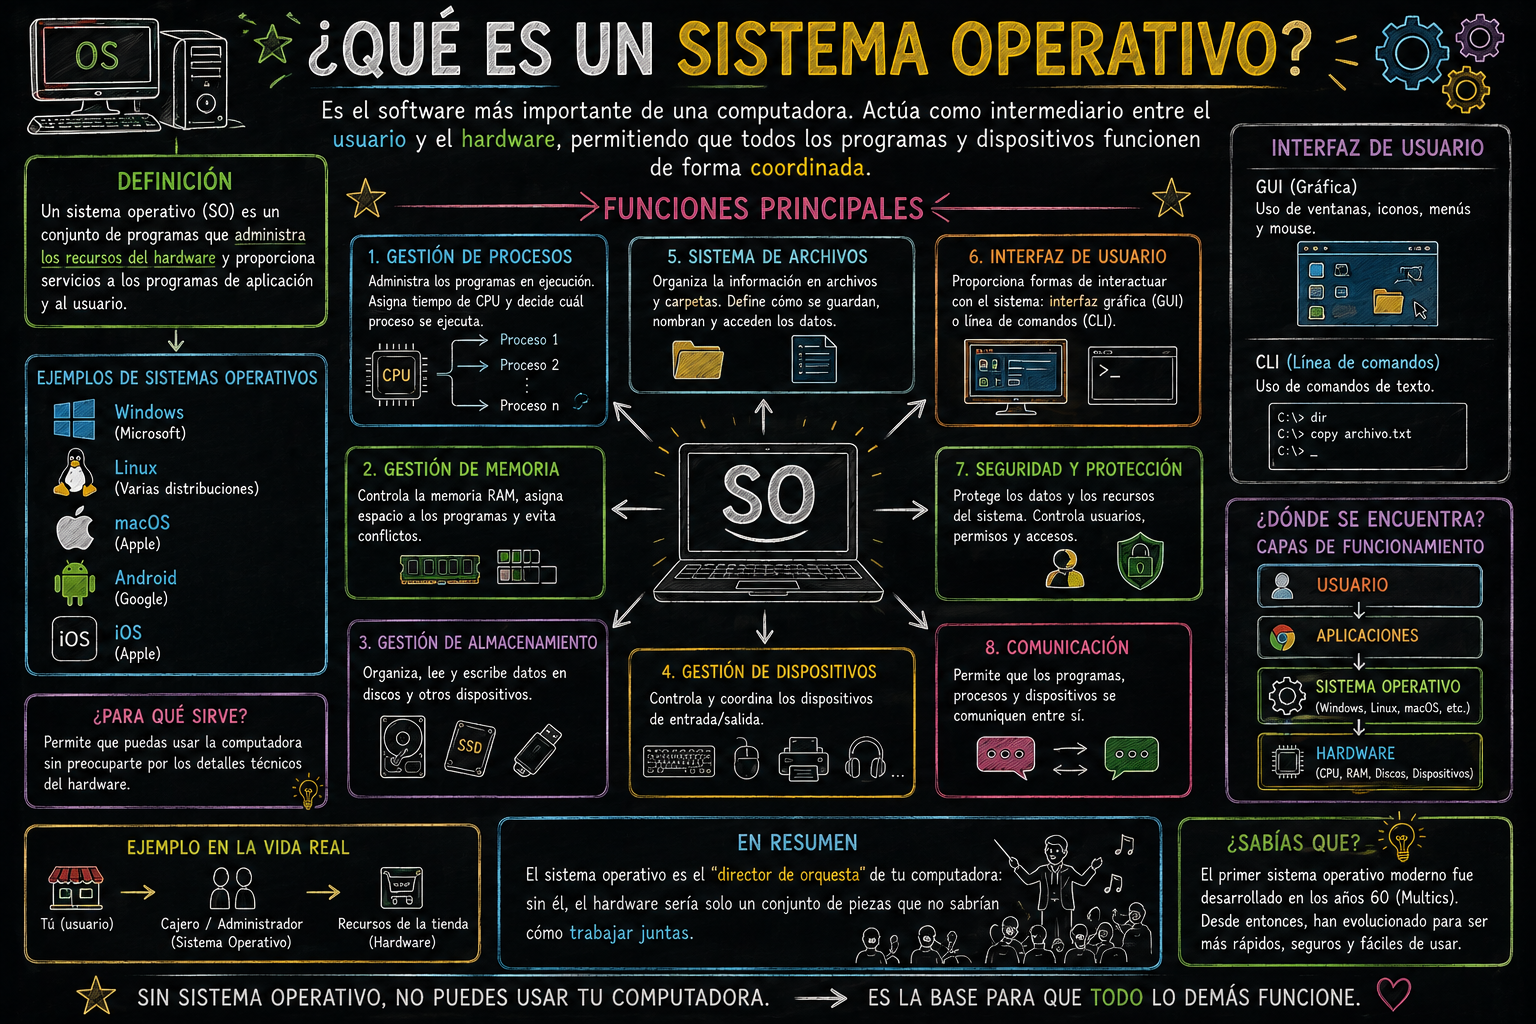
\includegraphics[keepaspectratio]{figures/SO_overview.png}}

}

\caption{Imagen creada con ChatGPT.}

\end{figure}%

\section{\texorpdfstring{\textbf{SO actuales y sus
diferencias}}{SO actuales y sus diferencias}}\label{so-actuales-y-sus-diferencias}

\begin{figure}[H]

{\centering \pandocbounded{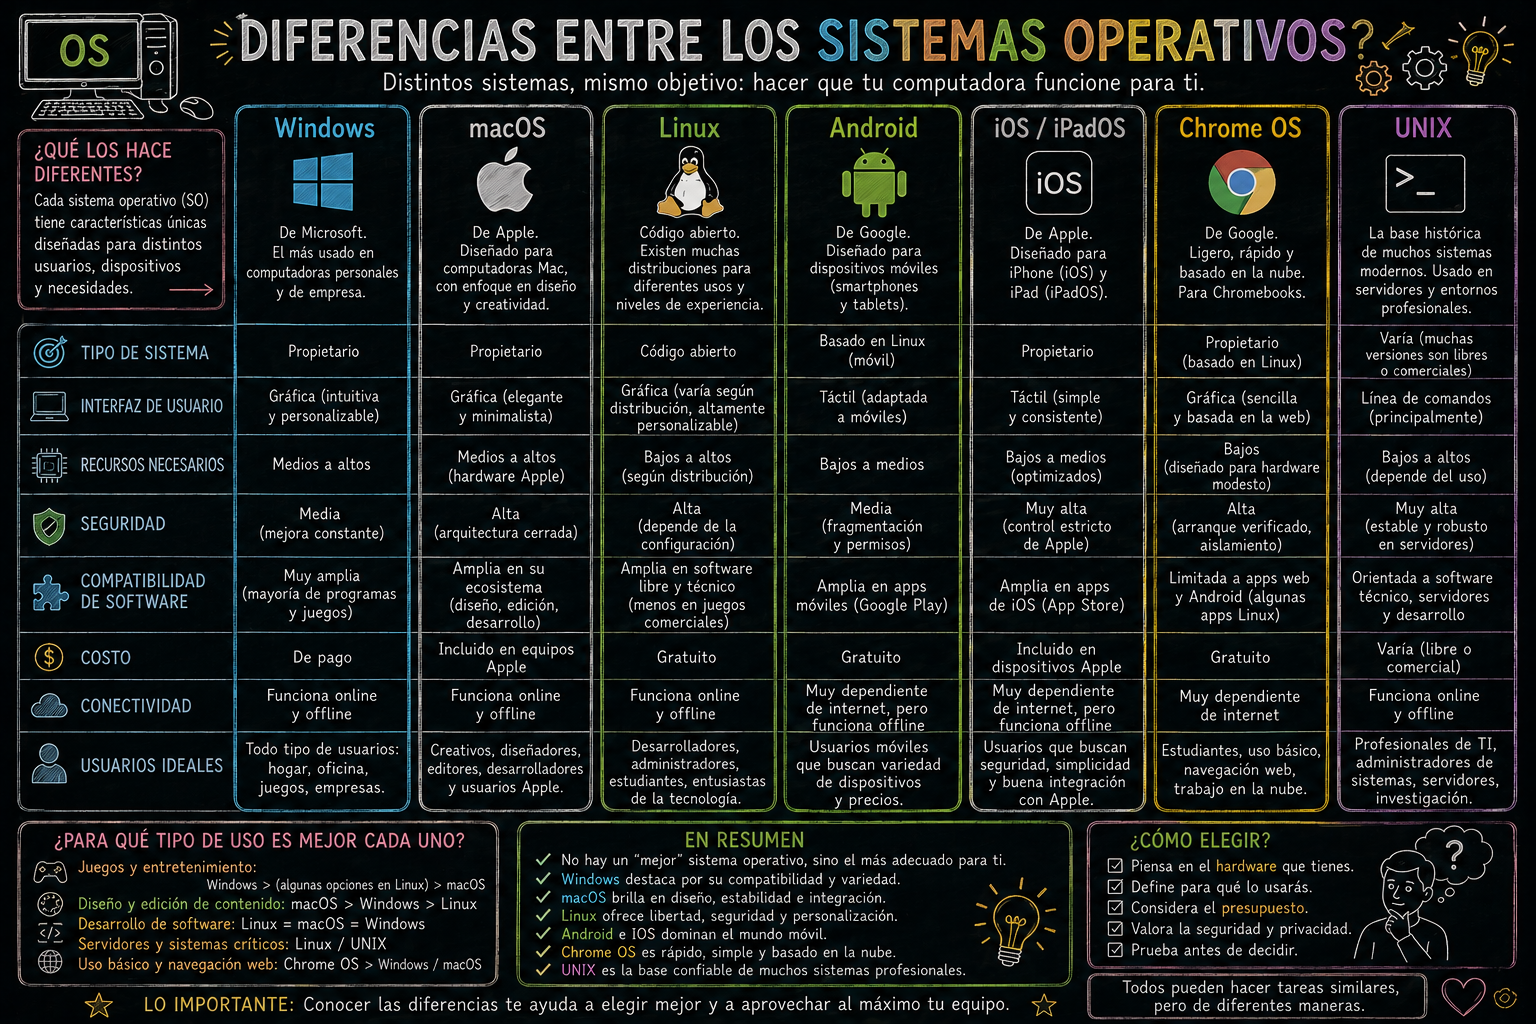
\includegraphics[keepaspectratio]{figures/SO_diferentes.png}}

}

\caption{Imagen creada con ChatGPT.}

\end{figure}%

Al final tu eliges cual usas y recuerda\ldots{}

\begin{center}
\pandocbounded{
\includegraphics[keepaspectratio]{figures/respuesta_corazon.jpg}}
\end{center}

\section{¿Qué son los drivers?}\label{quuxe9-son-los-drivers}

Es un software que actúa como traductor entre el Sistema Operativo y un
dispositivo de hardware.

\begin{figure}[H]

{\centering \pandocbounded{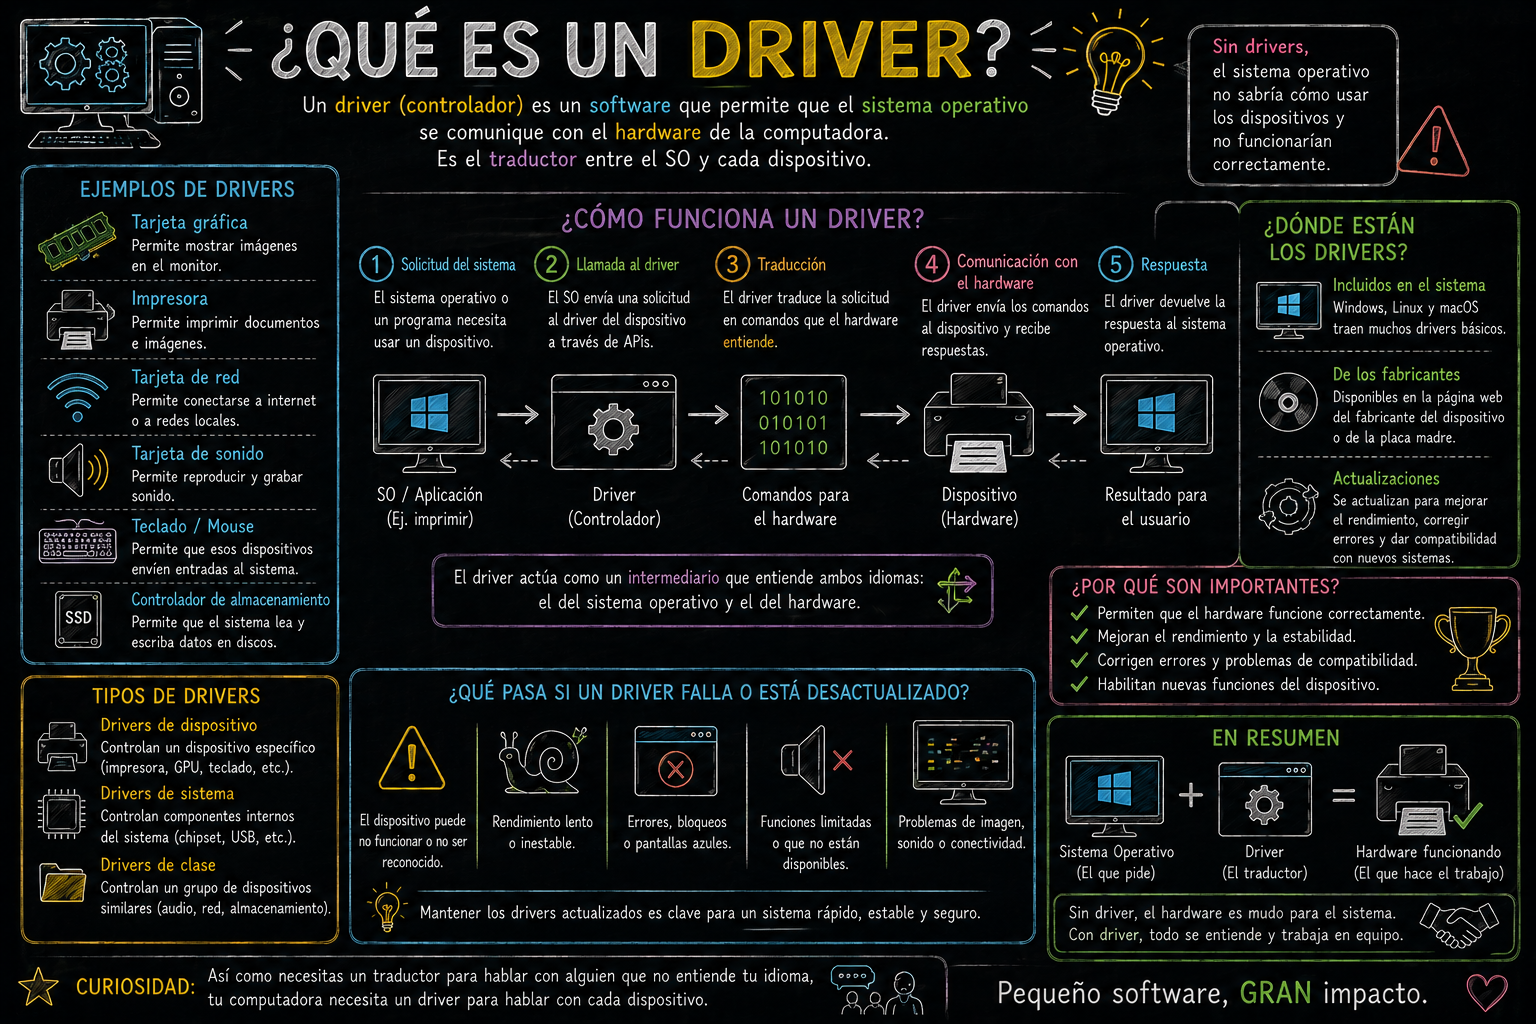
\includegraphics[keepaspectratio]{figures/SO_Drivers.png}}

}

\caption{Imagen creada con ChatGPT.}

\end{figure}%

\subsection{\texorpdfstring{\textbf{Drivers en diferentes
SO}}{Drivers en diferentes SO}}\label{drivers-en-diferentes-so}

\begin{verbatim}
🪟 Windows
├── Muchos drivers manuales
├── Windows Update los descarga
└── A veces necesitas instalarlos tú

🍎 macOS
├── Apple controla hardware y software
├── Drivers vienen integrados
└── Casi nunca necesitas instalar uno

🐧 Linux
├── Muchos drivers en el Kernel
├── Algunos requieren instalación manual
└── Hardware muy nuevo puede tener problemas
\end{verbatim}

\section{Reflexión grupal}\label{reflexiuxf3n-grupal}

\subsubsection{\texorpdfstring{\emph{¿Por qué macOS tiene menos
problemas de drivers que
Windows?}}{¿Por qué macOS tiene menos problemas de drivers que Windows?}}\label{por-quuxe9-macos-tiene-menos-problemas-de-drivers-que-windows}

\begin{figure}[H]

{\centering \pandocbounded{
\includegraphics[keepaspectratio]{figures/ReflexionGrupal_apple_vs_windows.png}}

}

\caption{Imagen creada con ChatGPT.}

\end{figure}%

\subsubsection{\texorpdfstring{\emph{¿Cómo afecta un driver de GPU
desactualizado al rendimiento en
videojuegos?}}{¿Cómo afecta un driver de GPU desactualizado al rendimiento en videojuegos?}}\label{cuxf3mo-afecta-un-driver-de-gpu-desactualizado-al-rendimiento-en-videojuegos}

Un driver desactualizado hace que la GPU no trabaje a su máximo
potencial, causando menos FPS, errores visuales y crashes.

\begin{tcolorbox}[enhanced jigsaw, arc=.35mm, bottomrule=.15mm, bottomtitle=1mm, breakable, colback=white, colbacktitle=quarto-callout-note-color!10!white, colframe=quarto-callout-note-color-frame, coltitle=black, left=2mm, leftrule=.75mm, opacityback=0, opacitybacktitle=0.6, rightrule=.15mm, title=\textcolor{quarto-callout-note-color}{\faInfo}\hspace{0.5em}{¿Qué es FPS?}, titlerule=0mm, toprule=.15mm, toptitle=1mm]

Es cuántas imágenes por segundo genera tu GPU en un videojuego

\begin{verbatim}
FPS = Frames Per Second
    = Fotogramas Por Segundo

30 FPS  → Jugable pero no fluido 🐢
60 FPS  → Fluido y cómodo ✅
120 FPS → Muy fluido ⚡
240 FPS → Competitivo profesional 🏆

Más FPS = Juego más fluido y suave
Menos FPS = Juego entrecortado y lento
\end{verbatim}

\end{tcolorbox}

\begin{figure}[H]

{\centering \pandocbounded{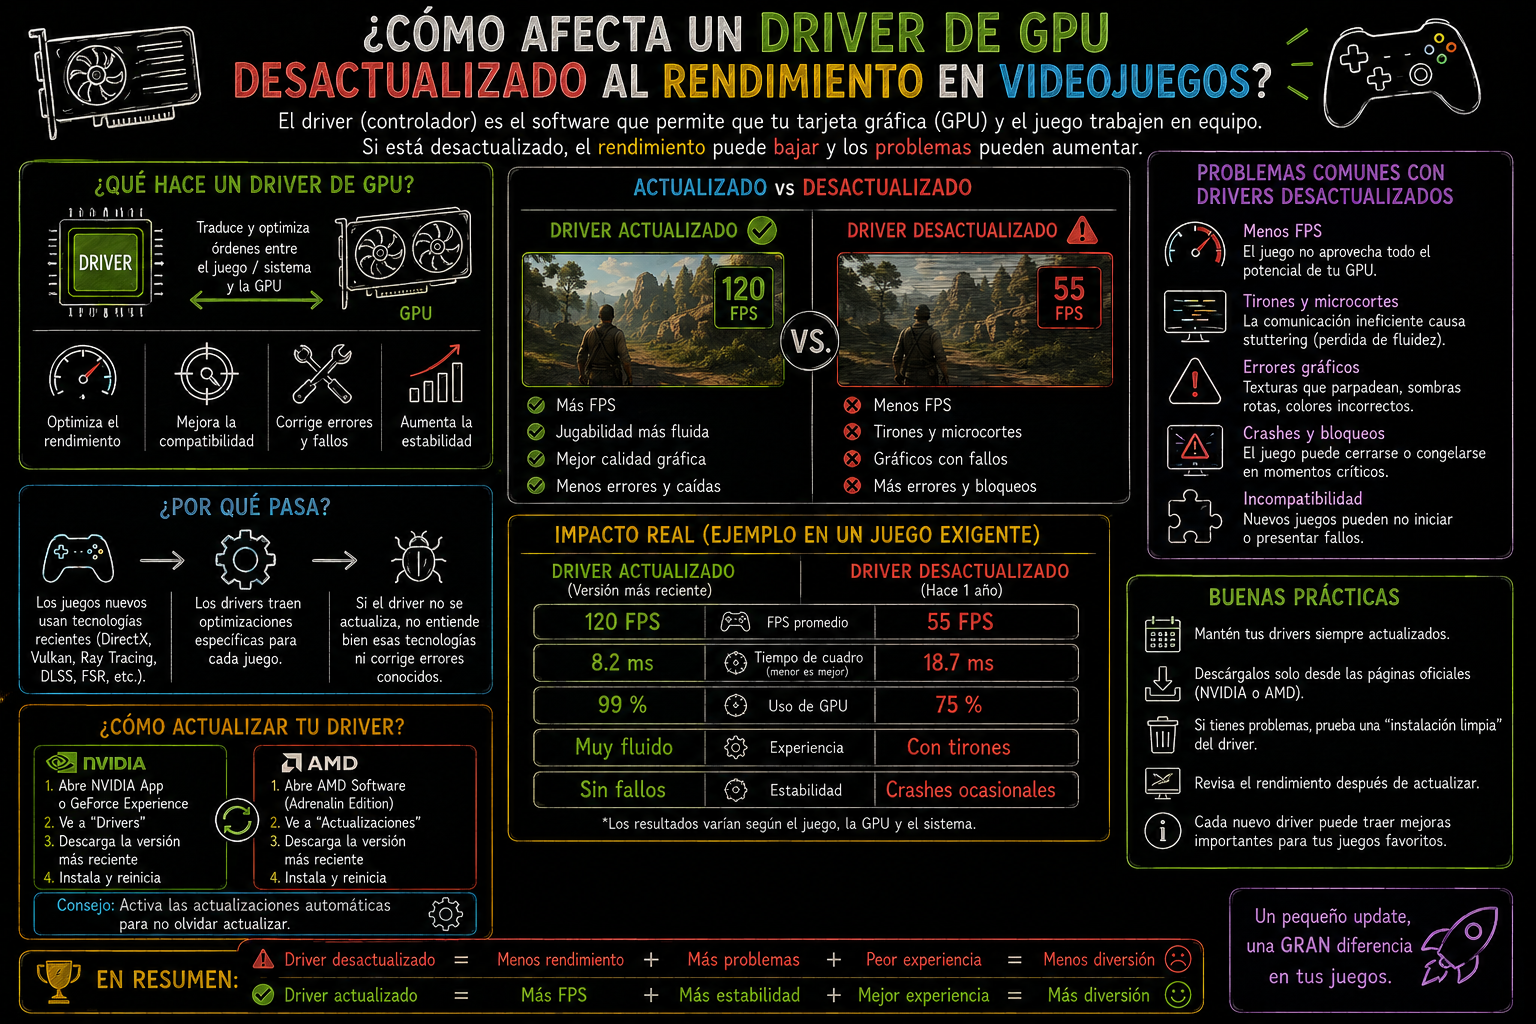
\includegraphics[keepaspectratio]{figures/ReflexionGrupal_fps.png}}

}

\caption{Imagen creada con ChatGPT.}

\end{figure}%

\chapter{\texorpdfstring{\textbf{✏️ Tarea 1 -} Mi Sistema
Operativo}{✏️ Tarea 1 - Mi Sistema Operativo}}\label{tarea-1---mi-sistema-operativo}

\begin{quote}
\textbf{Fecha de publicación:} jueves 03 de septiembre, 2026

\textbf{Fecha de entrega:} lunes 07 de septiembre, 2026
\end{quote}

Investigación de Sistemas Operativos

\textbf{Enunciado:}

\begin{verbatim}
TAREA 1: "Mi Sistema Operativo"

Objetivo: Investigar y documentar el SO que usas actualmente

Instrucciones:
1. Identifica el SO que usas en tu computadora
2. Investiga y responde:
   a) ¿Cuál es el nombre completo del SO?
   b) ¿Cuál es la versión que tienes instalada?
   c) ¿Cuándo se lanzó la primera versión?
   d) ¿Quién lo desarrolló?
   e) ¿Cuáles son sus características principales?
   f) ¿Por qué elegiste este SO?

3. Crea un documento (Word, Google Docs o PDF) con:
   - Título: "Mi Sistema Operativo -  Nombre del estudiante"
   - Respuestas a las preguntas anteriores
   - Una captura de pantalla de tu SO
   - Mínimo 300 palabras

4. Sube el documento a Google Classroom

Recursos:
- Puedes usar Doc para ayudarte a estructurar tu investigación
- Consulta sitios oficiales del SO (microsoft.com, apple.com, ubuntu.com)

Criterios de Evaluación:
- Completitud de respuestas (40%)
- Claridad y organización (30%)
- Captura de pantalla incluida (20%)
- Ortografía y gramática (10%)
\end{verbatim}

\textbf{Duración Estimada:} 45 minutos

\textbf{Apoyo de Doc:}

\begin{itemize}
\tightlist
\item
  Estudiante consulta a Doc: ``¿Cómo investigo mi SO?''
\item
  Doc proporciona estructura y preguntas guía
\item
  Doc ayuda a organizar la información
\end{itemize}

\section{Referencias}\label{referencias-2}

\begin{itemize}
\tightlist
\item
  Preguntale a Doc desde Google classroom.
\end{itemize}

\chapter{Buenas prácticas en
programación}\label{buenas-pruxe1cticas-en-programaciuxf3n}

\begin{quote}
\textbf{Fecha:} 03 de septiembre, 2026
\end{quote}

\textbf{Objetivos:}

\begin{enumerate}
\def\labelenumi{\arabic{enumi}.}
\tightlist
\item
  Conocer las buenas prácticas
\item
  Valorar la importancia del software libre y de código abierto
\item
  Aplicar este conocimiento en la selección de sistemas operativos
\end{enumerate}

Notas personales recabadas a partir de los tutoriales y ejemplos 😊.
Espero que les funcione 💜

\section{\texorpdfstring{\textbf{Un algoritmo nos permite resolver un
problema
⭐}}{Un algoritmo nos permite resolver un problema ⭐}}\label{un-algoritmo-nos-permite-resolver-un-problema}

Un algoritmo es un \textbf{conjunto de pasos lógicos y ordenados} que
describe cómo resolver un problema específico. Es una secuencia de
instrucciones abstractas e independientes del lenguaje de programación.

Características:

\begin{itemize}
\tightlist
\item
  {\textbf{Definido (Determinístico)}}: Un algoritmo es
  \textbf{definido} si al seguirlo dos veces con los mismos datos de
  entrada, siempre se obtiene el \textbf{mismo resultado}. Es
  \textbf{reproducible} y predecible.

  \begin{itemize}
  \tightlist
  \item
    \textbf{Implicaciones:}

    \begin{itemize}
    \tightlist
    \item
      No hay ambigüedad en los pasos
    \item
      No depende del azar o de factores externos
    \item
      Cualquier persona que siga el algoritmo llegará al mismo resultado
    \end{itemize}
  \end{itemize}
\item
  {\textbf{Preciso (Orden Específico)}}: implica el orden de realización
  de cada uno de los pasos. No puedes cambiar el orden arbitrariamente
  sin afectar el resultado.

  \begin{itemize}
  \tightlist
  \item
    \textbf{Implicaciones:}

    \begin{itemize}
    \tightlist
    \item
      Cada paso debe ejecutarse en el orden correcto
    \item
      El orden es fundamental para obtener el resultado esperado
    \item
      Las instrucciones deben ser claras y sin ambigüedad
    \end{itemize}
  \end{itemize}
\item
  {\textbf{Finito (Tiene un Fin)}}: Tiene un numero determinado de pasos
  y siempre termina en algún momento. No puede ejecutarse
  indefinidamente.

  \begin{itemize}
  \tightlist
  \item
    \textbf{Implicaciones:}

    \begin{itemize}
    \item
      Debe haber un punto de salida o conclusión
    \item
      No puede entrar en bucles infinitos
    \item
      Debe producir un resultado en tiempo finito
    \end{itemize}
  \end{itemize}
\end{itemize}

\begin{quote}
\begin{itemize}
\tightlist
\item
  \textbf{Algoritmo} = La idea y el plan (abstracto)
\item
  \textbf{Programa/Software} = La implementación concreta (código
  ejecutable)
\end{itemize}
\end{quote}

\begin{figure}[H]

{\centering \pandocbounded{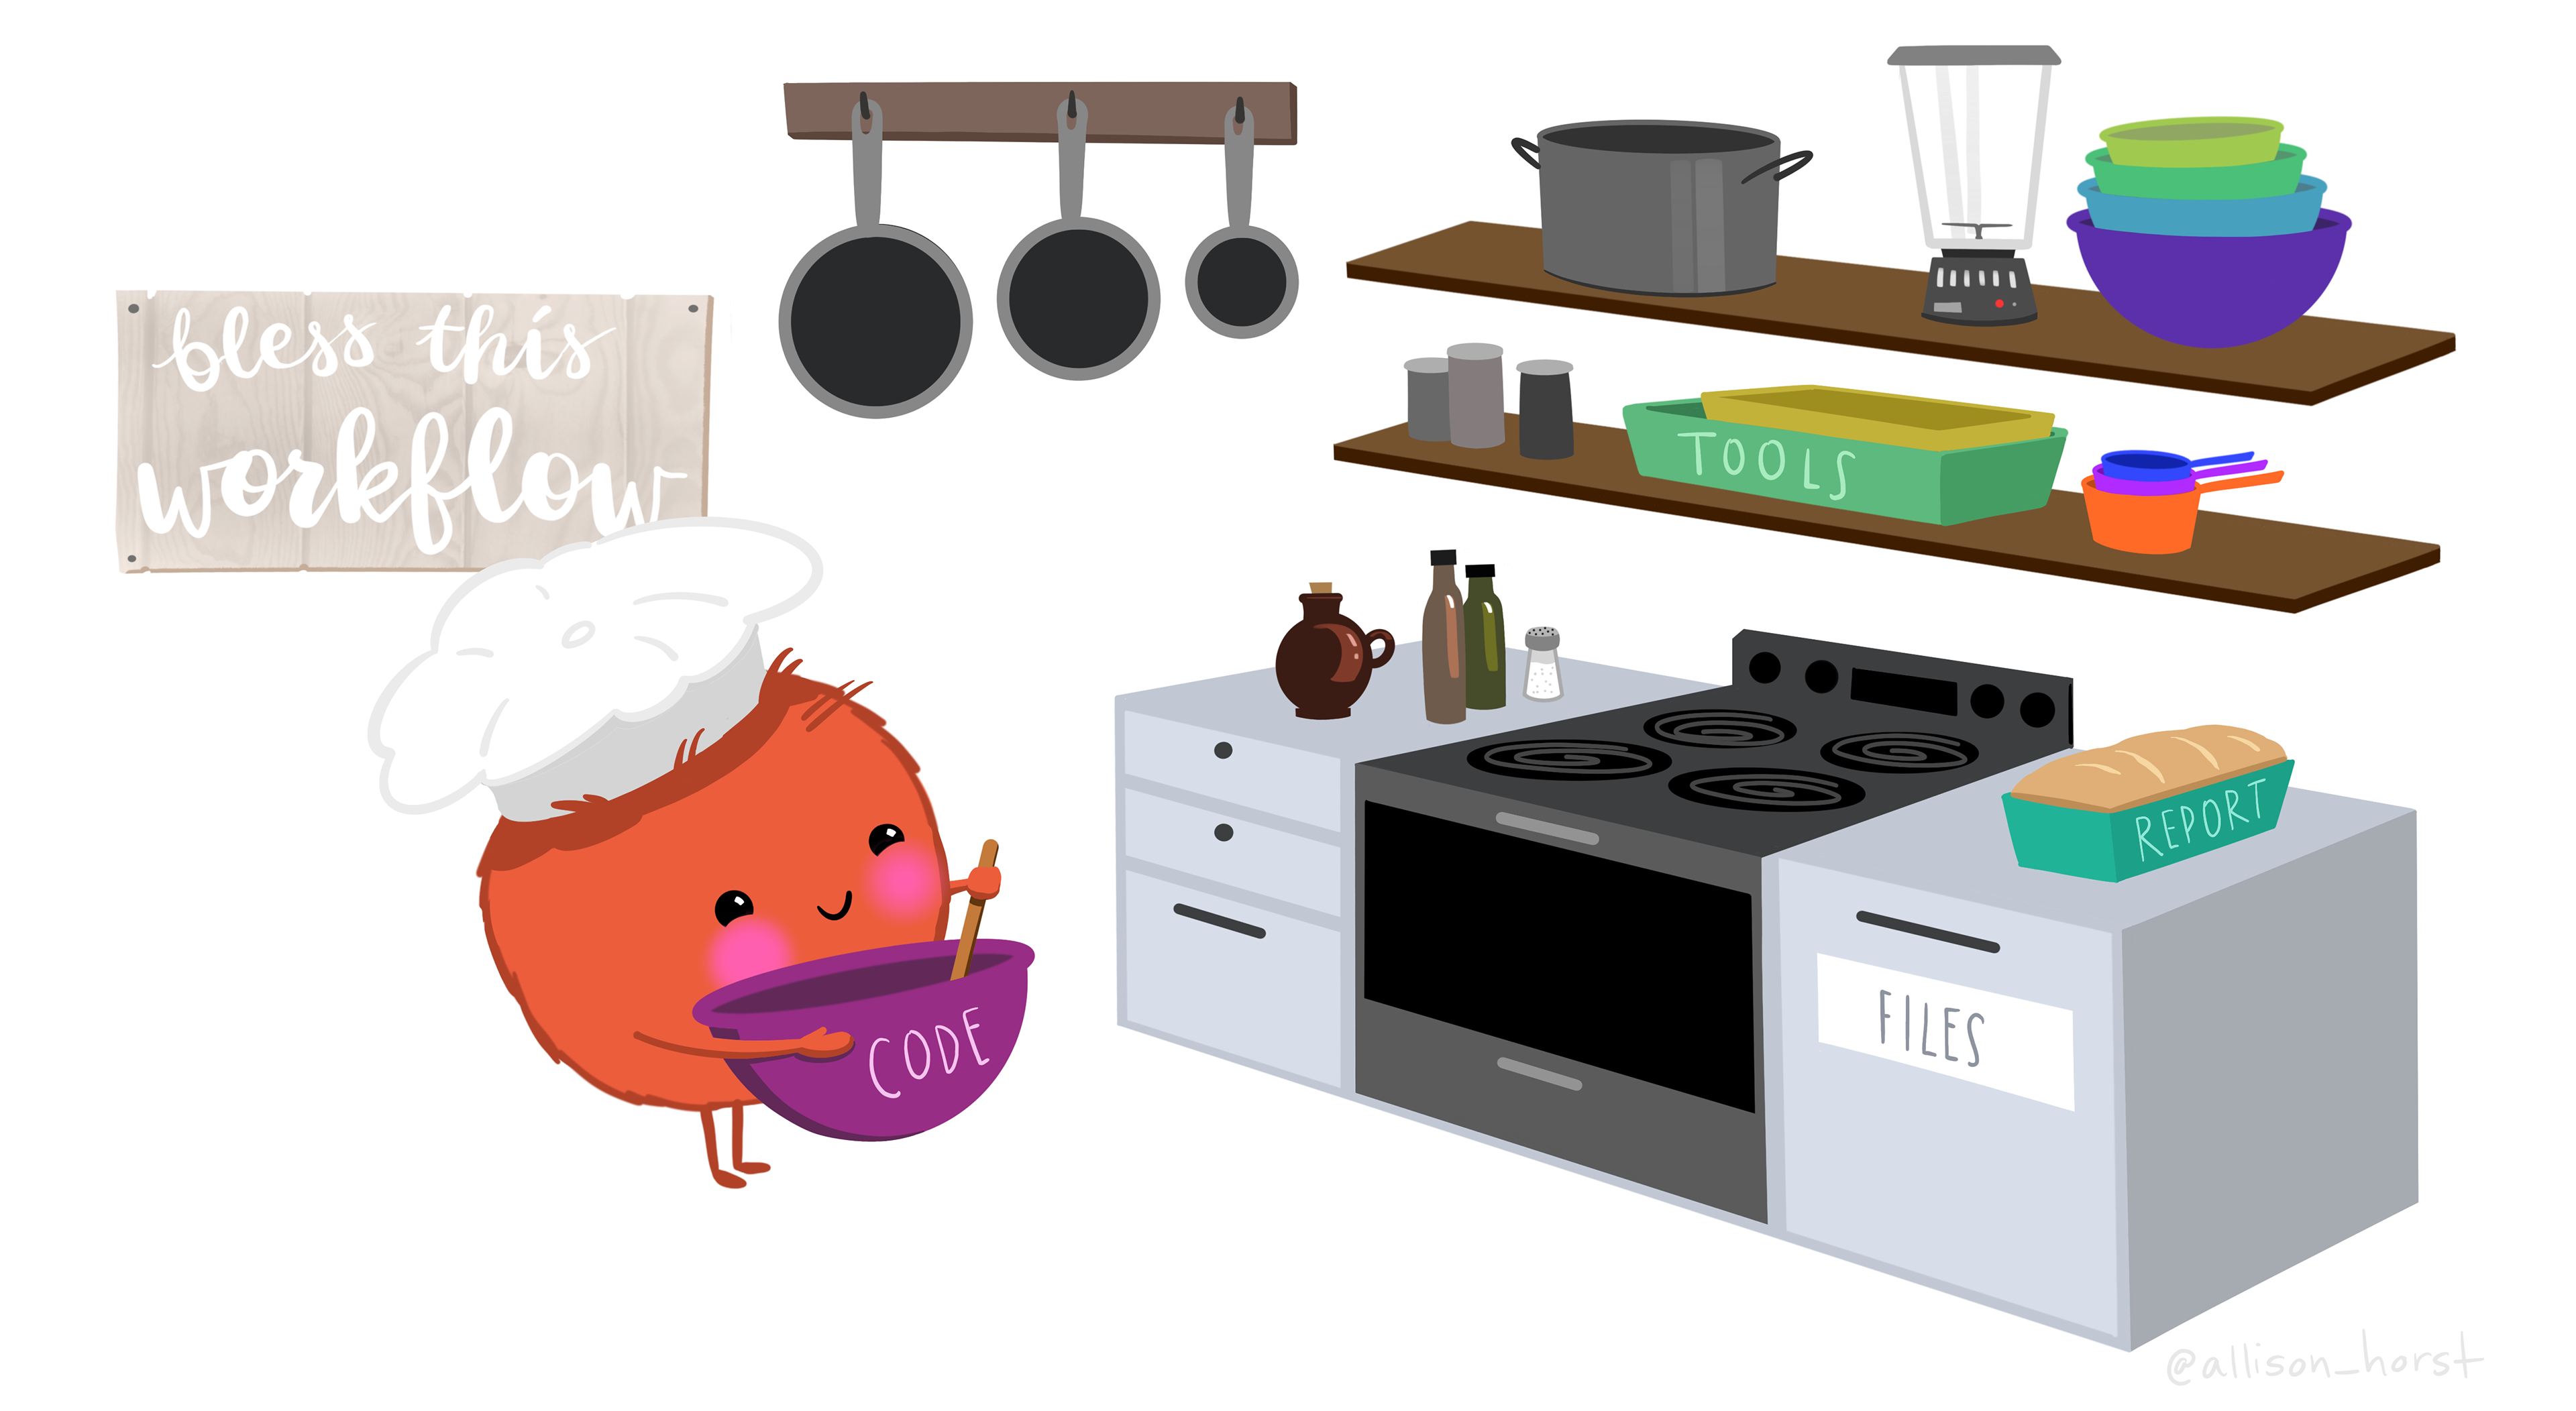
\includegraphics[keepaspectratio]{figures/allison-horst-code-kitchen.png}}

}

\caption{Imagen obtenida de sitio web de Allison Horst.}

\end{figure}%

\begin{tcolorbox}[enhanced jigsaw, arc=.35mm, bottomrule=.15mm, bottomtitle=1mm, breakable, colback=white, colbacktitle=quarto-callout-important-color!10!white, colframe=quarto-callout-important-color-frame, coltitle=black, left=2mm, leftrule=.75mm, opacityback=0, opacitybacktitle=0.6, rightrule=.15mm, title=\textcolor{quarto-callout-important-color}{\faExclamation}\hspace{0.5em}{Importante}, titlerule=0mm, toprule=.15mm, toptitle=1mm]

Los algoritmos son conceptuales y puede expresarse en \textbf{lenguaje
natural, pseudocódigo o diagramas de flujo.}

\end{tcolorbox}

\section{\texorpdfstring{\textbf{🗣️ Lenguaje
Natural}}{🗣️ Lenguaje Natural}}\label{lenguaje-natural}

\subsection{\texorpdfstring{\textbf{En el contexto de algoritmos y
programación}}{En el contexto de algoritmos y programación}}\label{en-el-contexto-de-algoritmos-y-programaciuxf3n}

\begin{itemize}
\tightlist
\item
  Utiliza \textbf{palabras comunes y cotidianas} para describir procesos
  o instrucciones.
\item
  Es \textbf{intuitivo y accesible,} ideal para explicar algoritmos sin
  tecnicismos.
\item
  No requiere conocimientos previos de programación.
\item
  Puede ser \textbf{ambiguo o impreciso,} por lo que no siempre es
  adecuado para implementación directa.
\item
  Se usa frecuentemente como primer paso antes de escribir pseudocódigo
  o código real.
\end{itemize}

\begin{tcolorbox}[enhanced jigsaw, arc=.35mm, bottomrule=.15mm, bottomtitle=1mm, breakable, colback=white, colbacktitle=quarto-callout-note-color!10!white, colframe=quarto-callout-note-color-frame, coltitle=black, left=2mm, leftrule=.75mm, opacityback=0, opacitybacktitle=0.6, rightrule=.15mm, title={Ejemplo de Lenguaje natural}, titlerule=0mm, toprule=.15mm, toptitle=1mm]

El programa solicita al usuario que ingrese su edad. Luego compara ese
valor con 18. Si la edad es \textbf{mayor o igual a 18}, se muestra el
mensaje ``Eres mayor de edad''. Si no lo es, se muestra ``Eres menor de
edad''.

\end{tcolorbox}

\section{\texorpdfstring{\textbf{Pseudocódigo}}{Pseudocódigo}}\label{pseudocuxf3digo}

\begin{itemize}
\tightlist
\item
  El pseudocódigo permite escribir algoritmos con \textbf{sintaxis
  relajada}, sin seguir reglas estrictas de un lenguaje de programación.
\item
  Organiza los \textbf{pasos lógicos} necesarios para construir un
  algoritmo, sin detallar estructuras de datos complejas.
\item
  Usa un \textbf{lenguaje sencillo y legible, accesible} para personas
  sin experiencia técnica.
\item
  🔄 Los pasos escritos en pseudocódigo pueden \textbf{traducirse
  fácilmente} a cualquier lenguaje de programación.
\end{itemize}

\begin{verbatim}
INICIO
  DEFINIR edad COMO ENTERO
  LEER edad
  SI edad >= 18 ENTONCES
    MOSTRAR "Eres mayor de edad"
  SINO
    MOSTRAR "Eres menor de edad"
FIN
\end{verbatim}

\section{\texorpdfstring{\textbf{Diagrama de
Flujo}}{Diagrama de Flujo}}\label{diagrama-de-flujo}

\begin{itemize}
\tightlist
\item
  Representa \textbf{visualmente un algoritmo mediante símbolos
  gráficos} (óvalos, rectángulos, rombos, etc.).
\item
  Muestra el flujo \textbf{lógico de decisiones, procesos y
  entradas/salidas.}
\item
  Facilita la \emph{comprensión rápida} de la estructura del algoritmo.
\item
  Ayuda a identificar errores o redundancias en la lógica.
\item
  Es útil tanto para documentación técnica como para enseñanza.
\end{itemize}

\pandocbounded{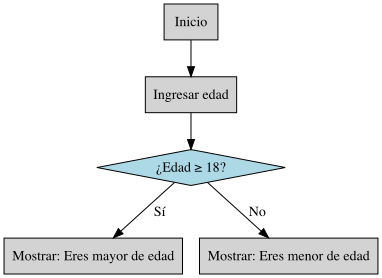
\includegraphics[keepaspectratio]{figures/diagrama_edad.png}}

\section{¿Qué es un código?}\label{quuxe9-es-un-cuxf3digo}

Se refiere a los \textbf{scripts, programas/software o fragmentos de
instrucciones escritas en lenguajes de programación} (como Python, R,
Bash, entre otros) que le indica a una computadora qué tareas realizar.

Es la forma en que los humanos comunicamos con las máquinas para
resolver problemas, procesar información y automatizar tareas.

Aplicaciones prácticas:

\begin{itemize}
\tightlist
\item
  Procesar y analizar datos
\item
  Crear visualizaciones
\item
  Resolver problemas matemáticos
\item
  Crear herramientas y aplicaciones
\item
  Documentar procesos
\end{itemize}

\begin{figure}[H]

{\centering \pandocbounded{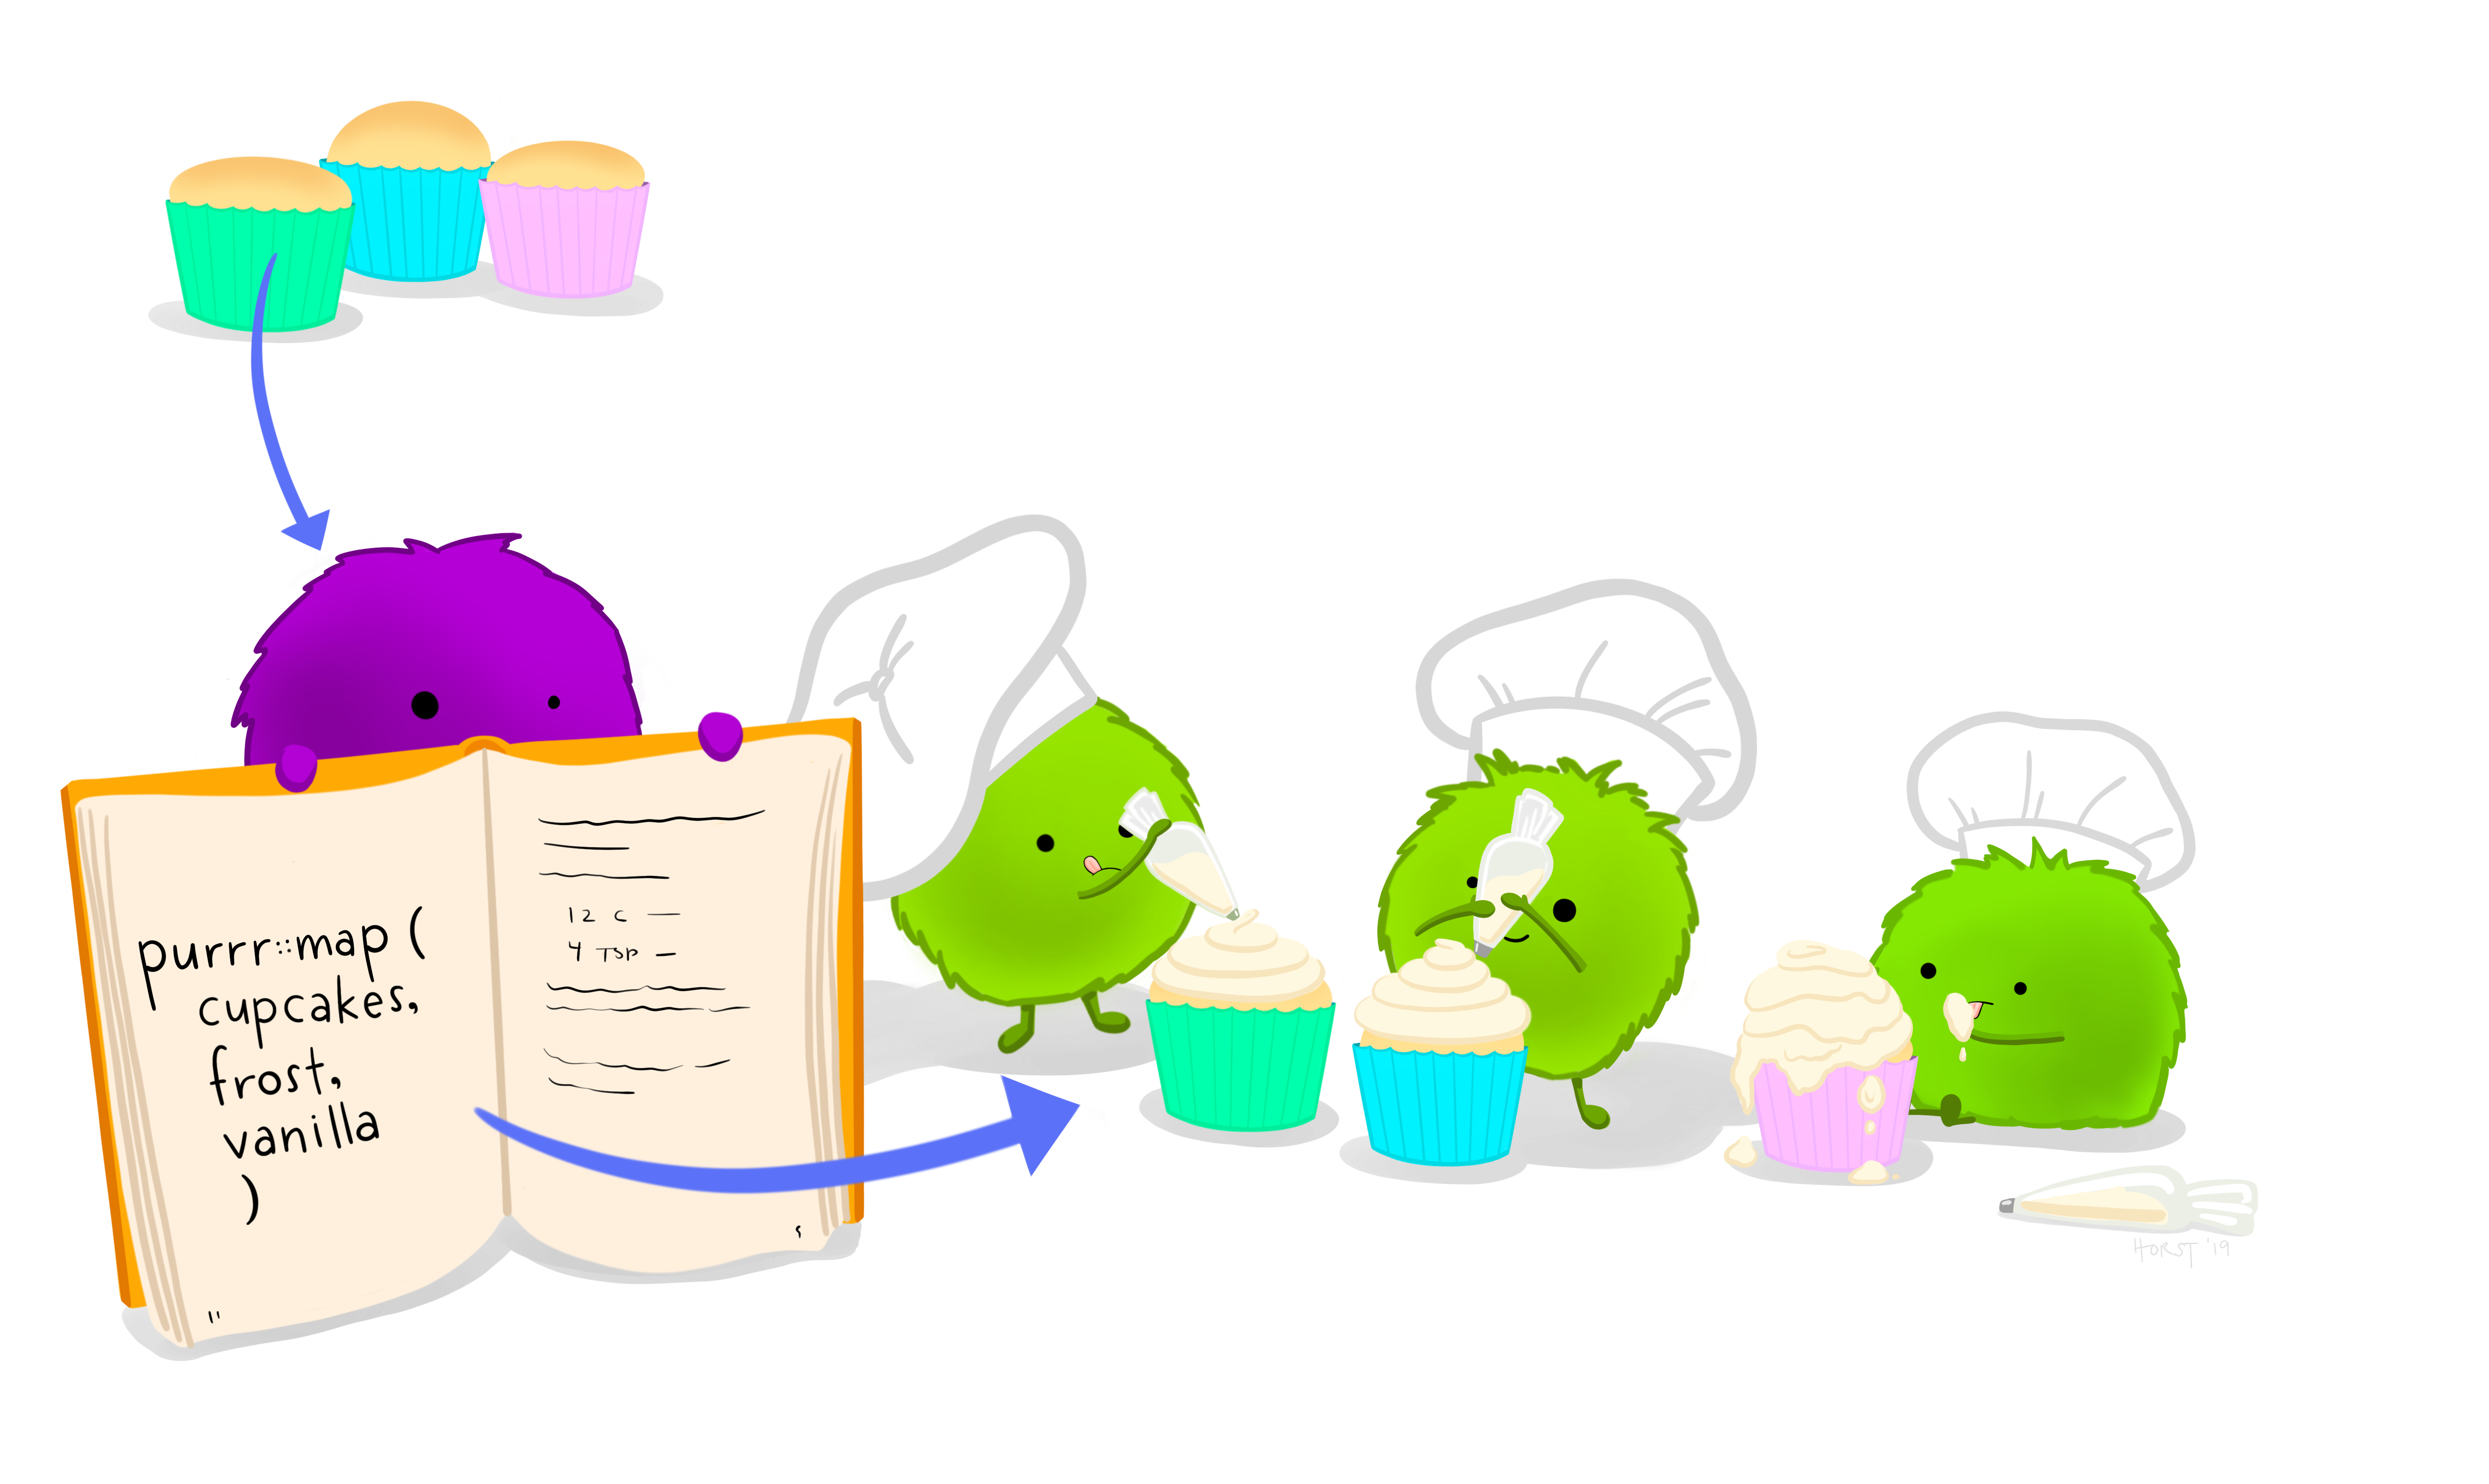
\includegraphics[keepaspectratio]{figures/codigo_pastel.png}}

}

\caption{Imagen obtenida de Allison Horst.}

\end{figure}%

\section{Para escribir un buen software
necesitas:}\label{para-escribir-un-buen-software-necesitas}

\begin{quote}
Escribir \textbf{código mantenible (maintainable code), usar control de
versiones (version control) y rastreadores de problemas (issue
trackers), revisiones de código (code reviews), pruebas unitarias (unit
testing) y automatización de tareas (task automation)}.

\href{https://journals.plos.org/plosbiology/article?id=10.1371/journal.pbio.1001745}{Wilson,
\emph{et al.} 2014. \emph{PLOS Biology}}
\end{quote}

\begin{figure}[H]

{\centering \pandocbounded{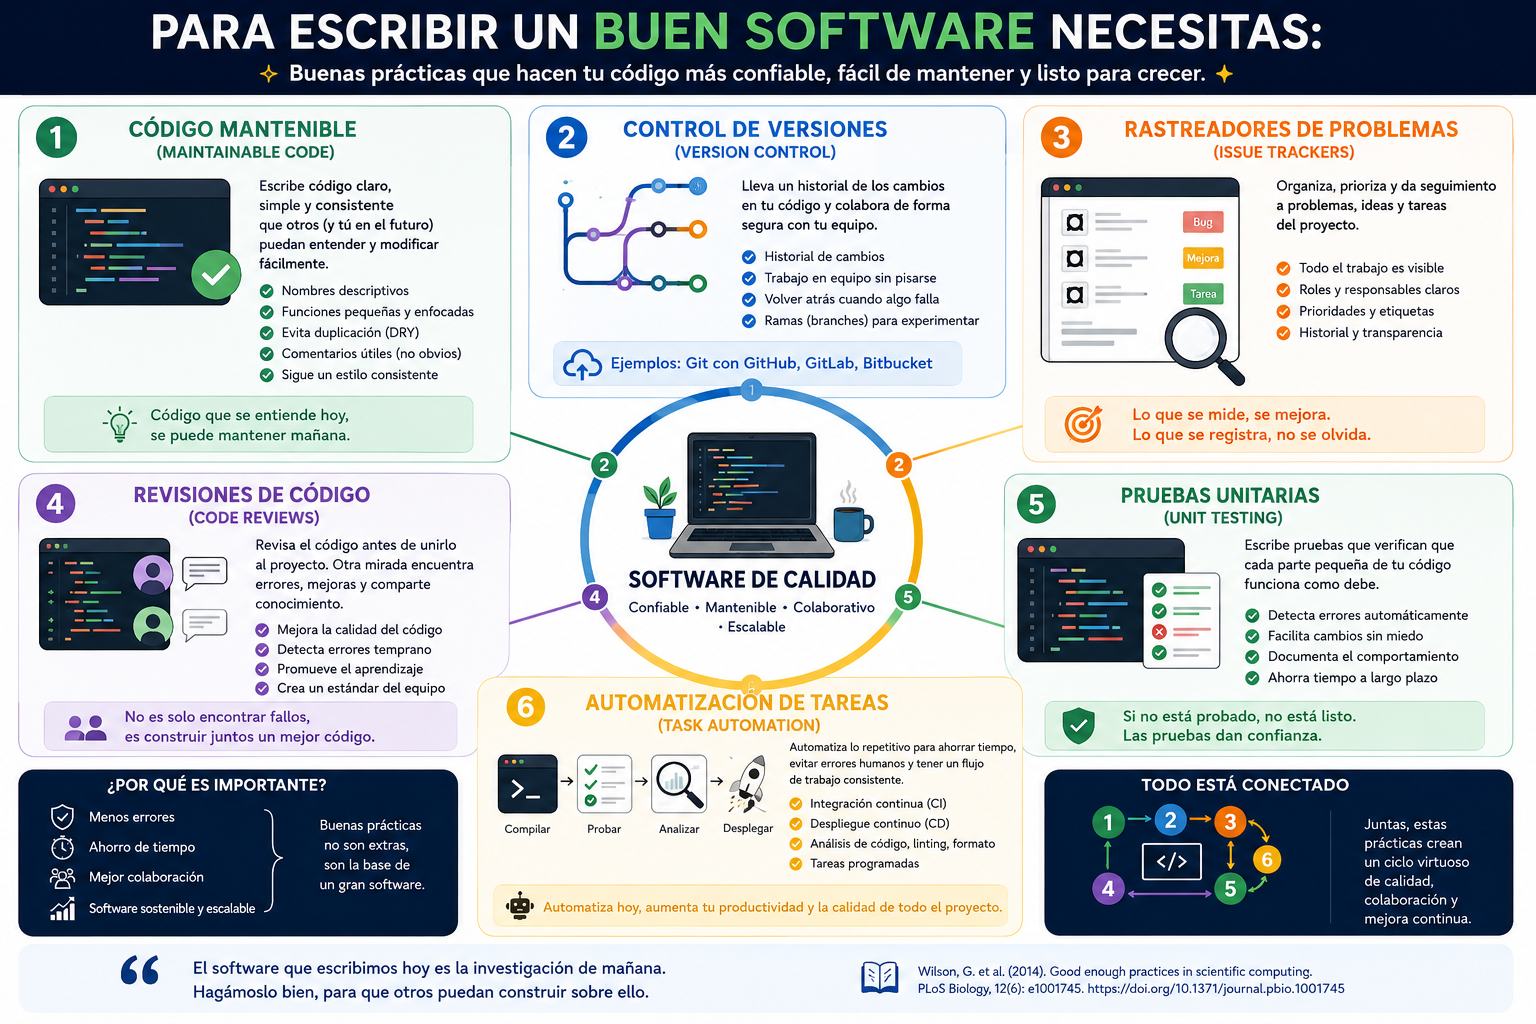
\includegraphics[keepaspectratio]{figures/buenaspracticas_buencodigo.png}}

}

\caption{Imagen creada con ChatGPT a partir del artículo de
\href{https://journals.plos.org/plosbiology/article?id=10.1371/journal.pbio.1001745}{Wilson,
\emph{et al.} 2014. \emph{PLOS Biology}}\emph{.}}

\end{figure}%

\section{Pasos para escribir un buen
software}\label{pasos-para-escribir-un-buen-software}

\begin{figure}[H]

{\centering \pandocbounded{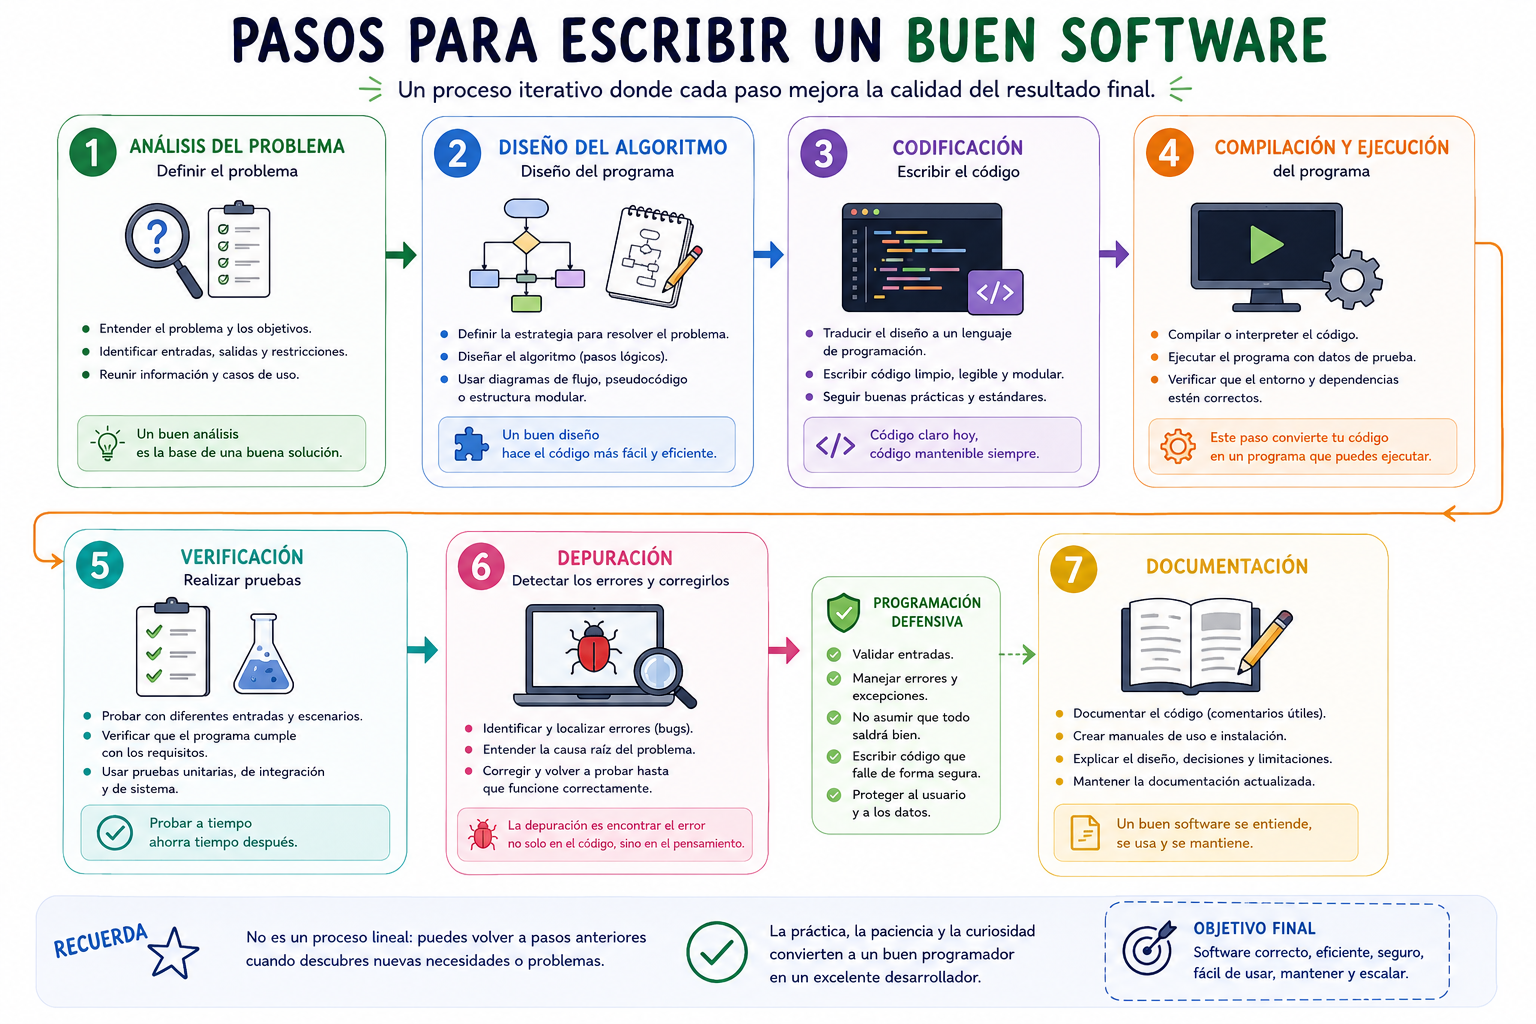
\includegraphics[keepaspectratio]{figures/buenaspracticas_pasos.png}}

}

\caption{Imagen creada con ChatGPT.}

\end{figure}%

\subsection{Mini historia de los bugs}\label{mini-historia-de-los-bugs}

El término ``bug'' (insecto en inglés) para referirse a errores en
programas tiene una historia curiosa y bien documentada que se remonta a
los primeros días de la computación.

En los años 1940s, las computadoras eran máquinas enormes que ocupaban
habitaciones completas, como la \textbf{ENIAC} (Electronic Numerical
Integrator and Computer). Estos equipos utilizaban miles de tubos de
vacío, relés y componentes electrónicos que generaban mucho calor.

\textbf{El problema:} Los insectos reales (polillas (moth), cucarachas y
otros bichos) eran atraídos por el calor de las máquinas y se metían
dentro de ellas, causando cortocircuitos y fallos en el funcionamiento.
🦗

Cuando los operadores encontraban estos insectos dentro de la máquina,
decían que había un ``bug'' (bicho) en el sistema. Así nació el término
de forma literal.

\begin{tcolorbox}[enhanced jigsaw, arc=.35mm, bottomrule=.15mm, bottomtitle=1mm, breakable, colback=white, colbacktitle=quarto-callout-note-color!10!white, colframe=quarto-callout-note-color-frame, coltitle=black, left=2mm, leftrule=.75mm, opacityback=0, opacitybacktitle=0.6, rightrule=.15mm, title=\textcolor{quarto-callout-note-color}{\faInfo}\hspace{0.5em}{¿Quién fue Grace Hopper?}, titlerule=0mm, toprule=.15mm, toptitle=1mm]

\textbf{Grace Brewster Murray Hopper} (1906-1992) fue una
\textbf{matemática, física y pionera de la programación} estadounidense
que revolucionó la forma en que escribimos software.

\end{tcolorbox}

\begin{figure}[H]

{\centering \pandocbounded{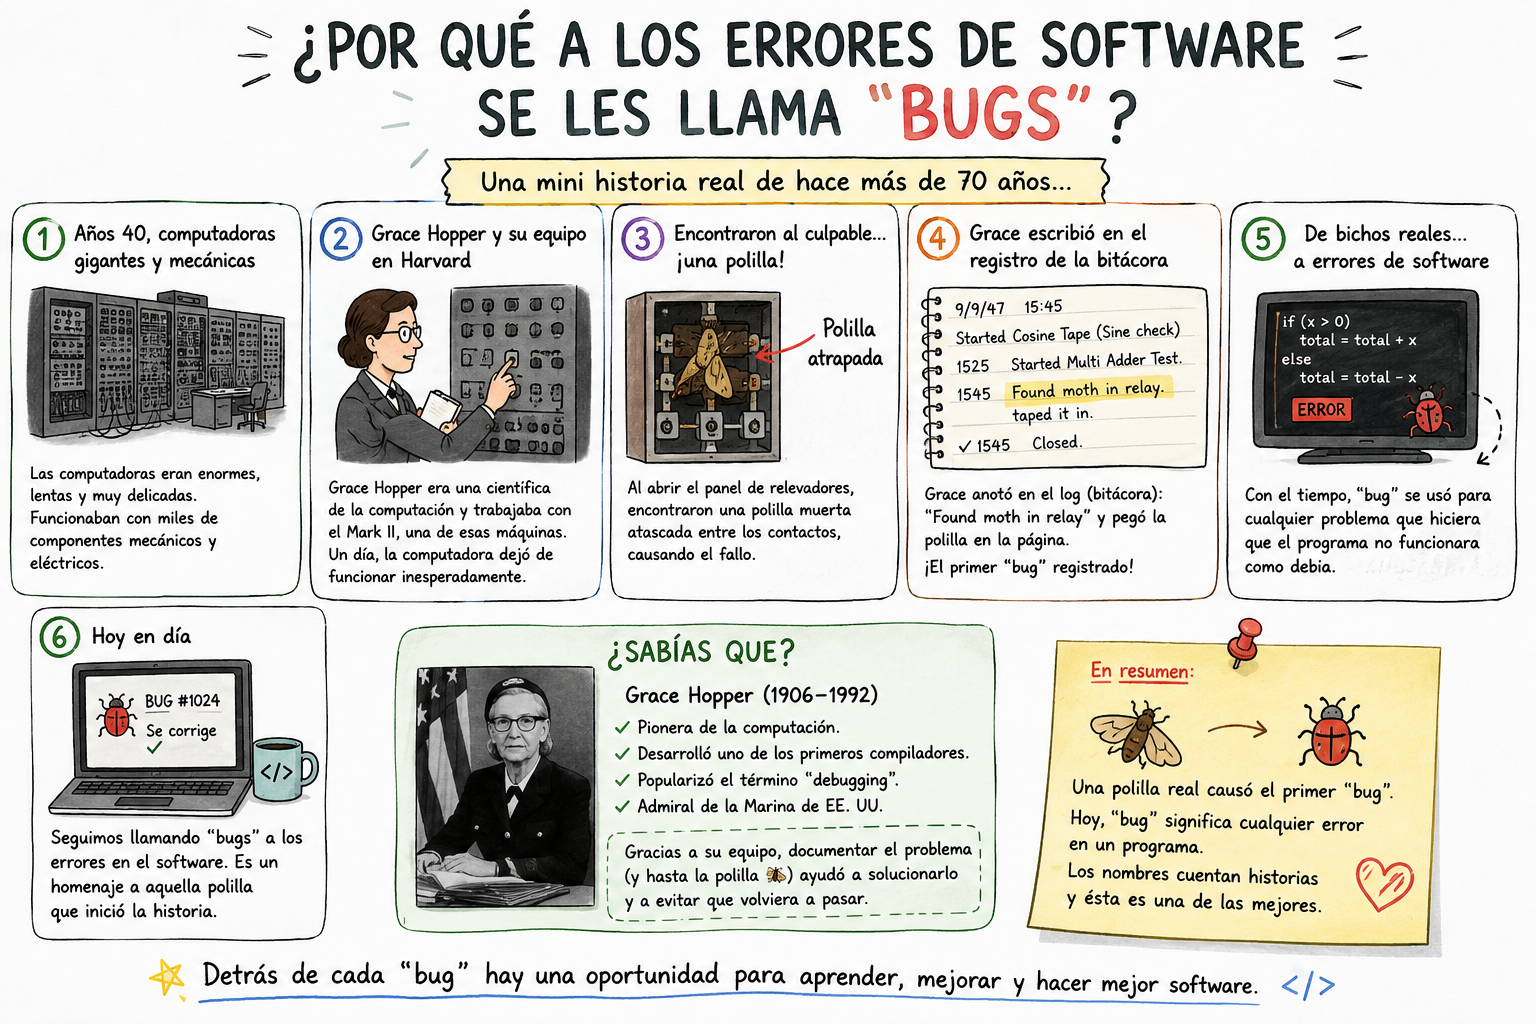
\includegraphics[keepaspectratio]{figures/mini_histoia_bugs.png}}

}

\caption{Imagen creada con ChatGPT.}

\end{figure}%

\begin{tcolorbox}[enhanced jigsaw, arc=.35mm, bottomrule=.15mm, bottomtitle=1mm, breakable, colback=white, colbacktitle=quarto-callout-note-color!10!white, colframe=quarto-callout-note-color-frame, coltitle=black, left=2mm, leftrule=.75mm, opacityback=0, opacitybacktitle=0.6, rightrule=.15mm, title=\textcolor{quarto-callout-note-color}{\faInfo}\hspace{0.5em}{¿Qué es ``Admiral''?}, titlerule=0mm, toprule=.15mm, toptitle=1mm]

Es un rango militar en la Marina de los Estados Unidos. Grace Hopper
alcanzó el rango de contraalmirante (Rear Admiral), uno de los más altos
para una mujer en esa época.

\end{tcolorbox}

\section{\texorpdfstring{\textbf{Lenguajes de programación
Comunes}}{Lenguajes de programación Comunes}}\label{lenguajes-de-programaciuxf3n-comunes}

{\def\LTcaptype{none} % do not increment counter
\begin{longtable}[]{@{}
  >{\raggedright\arraybackslash}p{(\linewidth - 4\tabcolsep) * \real{0.3333}}
  >{\raggedright\arraybackslash}p{(\linewidth - 4\tabcolsep) * \real{0.3333}}
  >{\raggedright\arraybackslash}p{(\linewidth - 4\tabcolsep) * \real{0.3333}}@{}}
\toprule\noalign{}
\begin{minipage}[b]{\linewidth}\raggedright
Lenguaje
\end{minipage} & \begin{minipage}[b]{\linewidth}\raggedright
Uso Principal
\end{minipage} & \begin{minipage}[b]{\linewidth}\raggedright
Ejemplo
\end{minipage} \\
\midrule\noalign{}
\endhead
\bottomrule\noalign{}
\endlastfoot
\textbf{\texttt{Bash}} & Automatización en sistemas Unix/Linux & Scripts
de sistema \\
\textbf{\texttt{Python}} & Ciencia de datos, automatización, educación &
Análisis de datos, machine learning \\
\textbf{\texttt{R}} & Análisis estadístico y visualización & Gráficos
científicos, estadística \\
\textbf{\texttt{JavaScript}} & Desarrollo web, aplicaciones interactivas
& Sitios web dinámicos \\
\textbf{\texttt{Java}} & Aplicaciones empresariales, sistemas grandes &
Software corporativo \\
\textbf{\texttt{C++}} & Sistemas de alto rendimiento & Videojuegos,
software de sistema \\
\textbf{\texttt{SQL}} & Gestión de bases de datos & Consultas de
datos \\
\end{longtable}
}

\subsection{\texorpdfstring{\textbf{Componentes
Básicos}}{Componentes Básicos}}\label{componentes-buxe1sicos}

{\def\LTcaptype{none} % do not increment counter
\begin{longtable}[]{@{}ll@{}}
\toprule\noalign{}
Componente & Descripción \\
\midrule\noalign{}
\endhead
\bottomrule\noalign{}
\endlastfoot
\textbf{Variables} & Espacios de memoria que almacenan datos \\
\textbf{Funciones} & Bloques de código reutilizables \\
\textbf{Condicionales} & Decisiones lógicas (si/entonces) \\
\textbf{Bucles} & Repetición de acciones \\
\textbf{Operadores} & Símbolos para realizar operaciones \\
\textbf{Comentarios} & Explicaciones para humanos \\
\end{longtable}
}

En este semestre veremos programación con \texttt{Bash}, \texttt{Python}
y un poco de \texttt{R}. Aquí es donde entra lo que aprendimos con
\emph{pseudocódigo}, ya que nos permite comprender y trasladar ideas a
través de los tres lenguajes.

\begin{figure}[H]

{\centering \pandocbounded{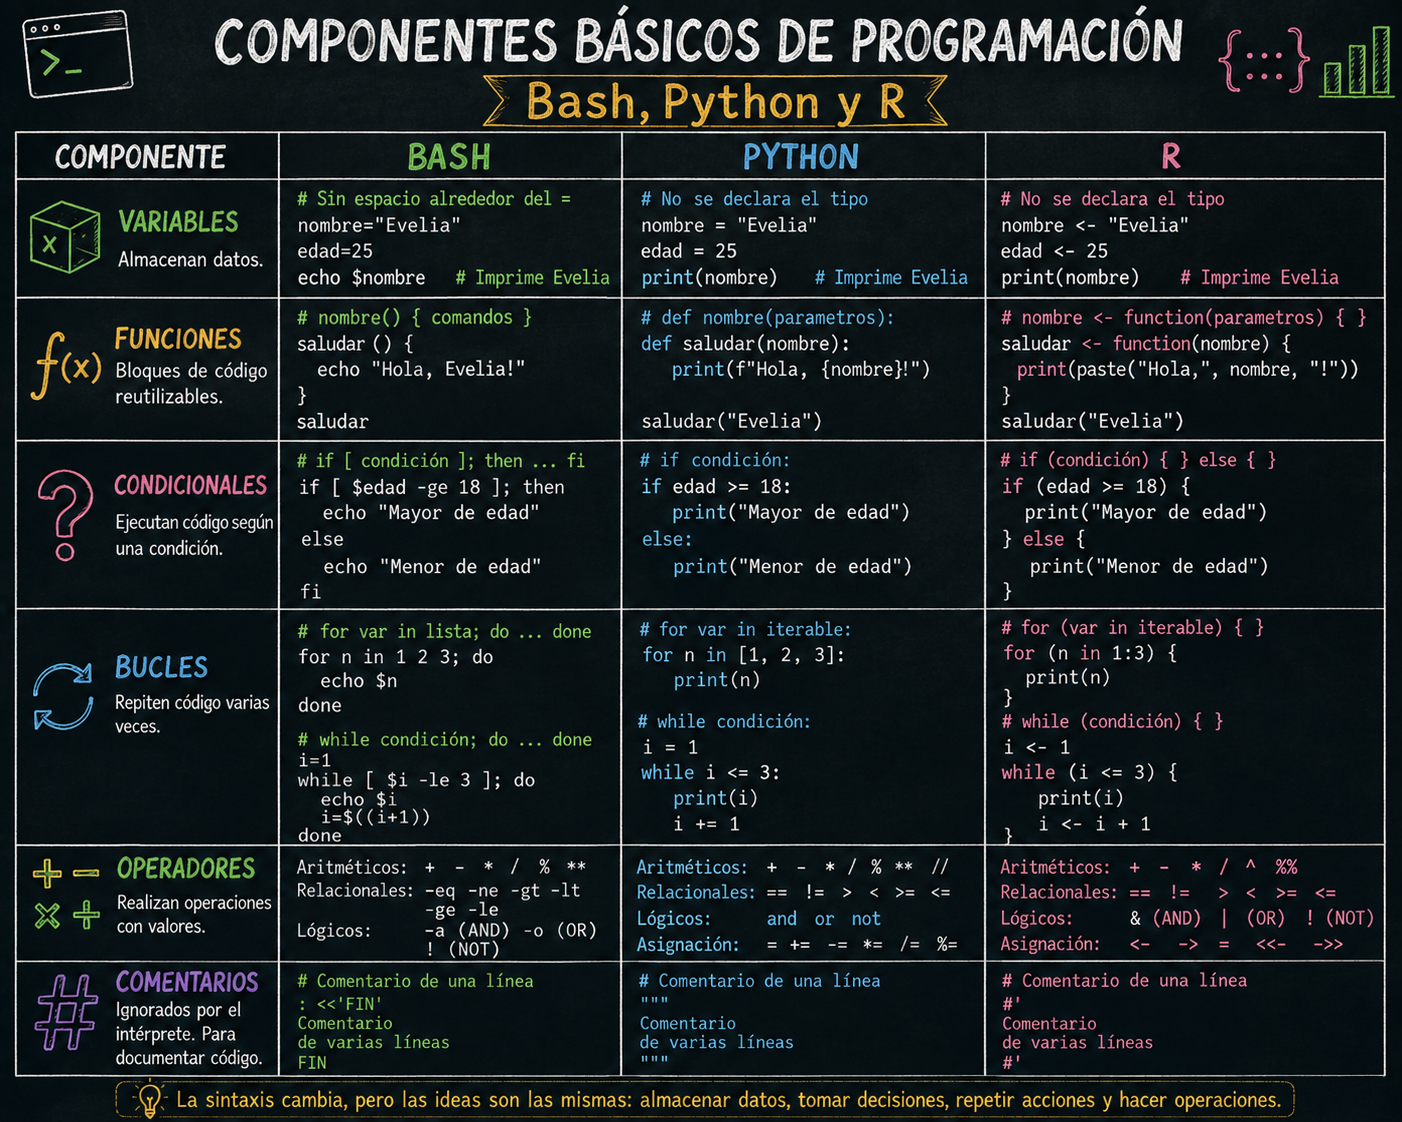
\includegraphics[keepaspectratio]{figures/lenguajes_overview.png}}

}

\caption{Imagen relaciona con los componentes básicos en los lenguajes
de programación que veremos, creada con ChatGPT.}

\end{figure}%

\section{Plantilla para la documentación de nuestro
código}\label{plantilla-para-la-documentaciuxf3n-de-nuestro-cuxf3digo}

\begin{tcolorbox}[enhanced jigsaw, arc=.35mm, bottomrule=.15mm, bottomtitle=1mm, breakable, colback=white, colbacktitle=quarto-callout-tip-color!10!white, colframe=quarto-callout-tip-color-frame, coltitle=black, left=2mm, leftrule=.75mm, opacityback=0, opacitybacktitle=0.6, rightrule=.15mm, title=\textcolor{quarto-callout-tip-color}{\faLightbulb}\hspace{0.5em}{Documentación de nuestro código}, titlerule=0mm, toprule=.15mm, toptitle=1mm]

\begin{itemize}
\item
  \emph{Título} (opcional)
\item
  \emph{Autor (author)}: Su nombre
\item
  \emph{Dia (date)}: Fecha de creación
\item
  \emph{Paquetes (packages)}
\item
  \emph{Directorio de trabajo (Working directory)}: En que carpeta se
  encuentra tu datos y programa.
\item
  \emph{Información descriptiva del programa (Description)}: ¿Para qué
  sirve el programa? Ej: El siguiente programa realiza la suma de dos
  numeros enteros a partir de la entrada del usuario y posteriormente la
  imprime en pantalla.
\item
  \emph{Usage} ¿Cómo se utiliza?
\item
  \emph{Argumentos (Arguments)}

  \begin{itemize}
  \item
    \emph{Información de entrada (Data Inputs)}: Ej: Solo numeros
    enteros (sin decimales).
  \item
    \emph{Información de salida (Outpus)}: Graficas, figuras, tablas,
    etc.
  \end{itemize}
\end{itemize}

\end{tcolorbox}

\begin{center}
\pandocbounded{\includegraphics[keepaspectratio]{index_files/mediabag/meme_documentacion.jpg}}
\end{center}

\section{Puntos claves para buenas prácticas en informática
⭐}\label{puntos-claves-para-buenas-pruxe1cticas-en-informuxe1tica}

\begin{figure}[H]

{\centering \pandocbounded{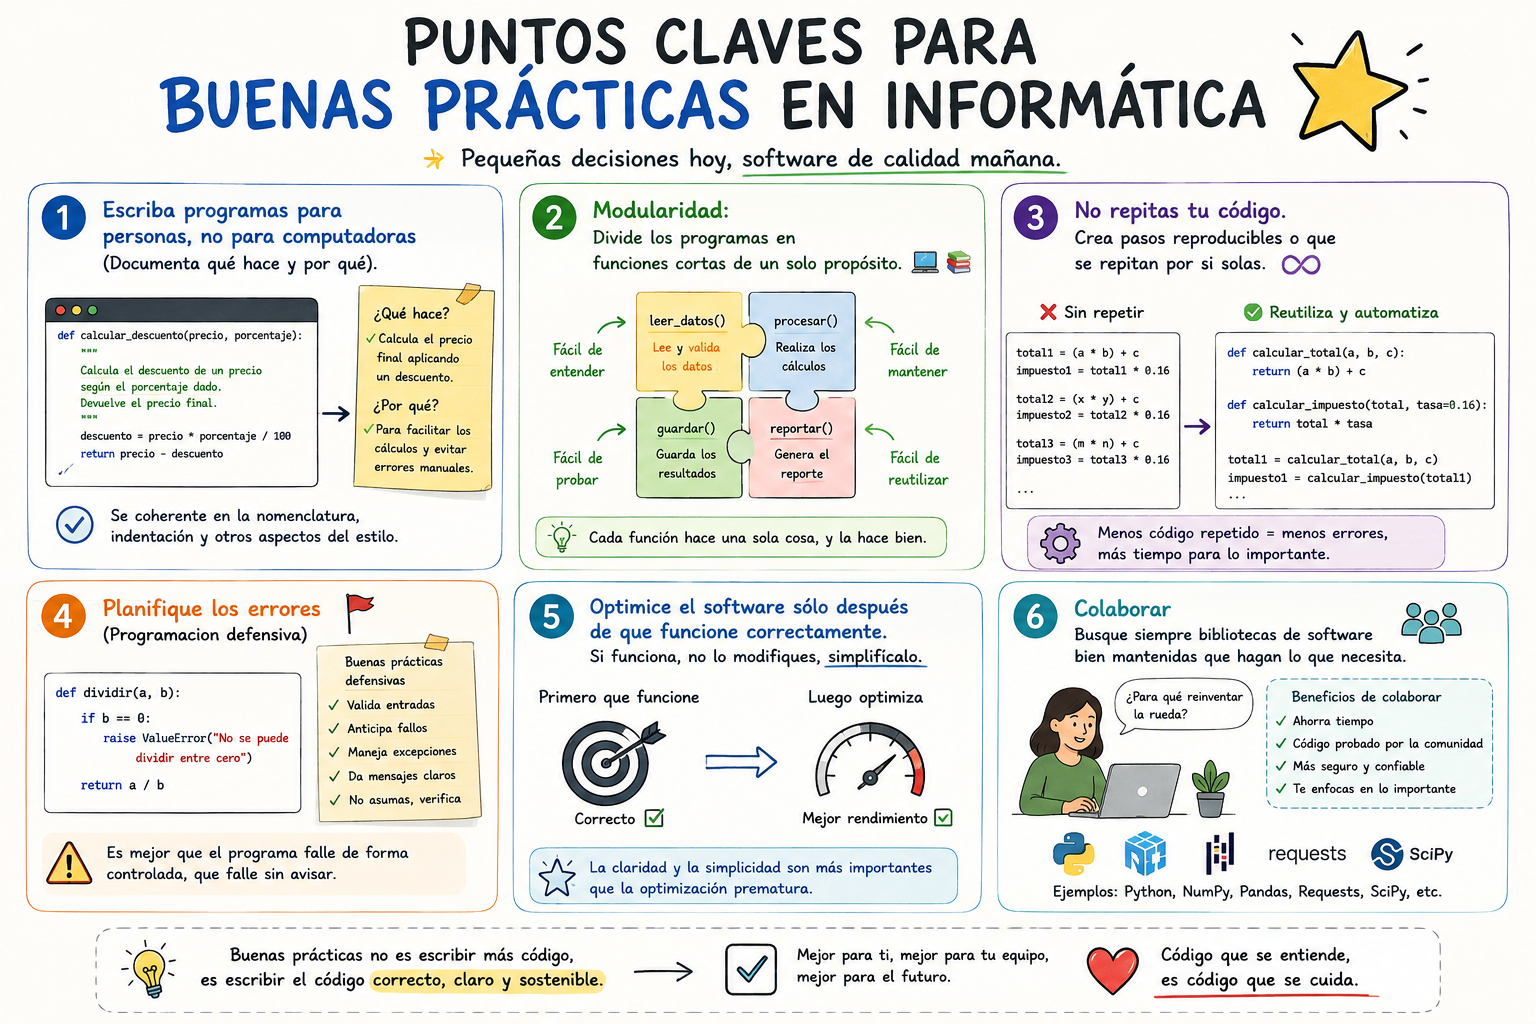
\includegraphics[keepaspectratio]{figures/buenaspracticas_summary.png}}

}

\caption{Imagen creada con ChatGPT.}

\end{figure}%

\section{Referencias}\label{referencias-3}

\begin{itemize}
\tightlist
\item
  Presentación de
  \href{https://miriamll.github.io/teaching_R_Rmd/Repro\#1}{Reproducibilidad
  de Miriam Lerma}
\item
  Presentación
  \href{https://miriamll.github.io/teaching_R_Rmd/GitGithubZenodo\#1}{introducción
  a Git, GitHub y Zenodo de Miriam Lerma}
\item
  \href{https://lcg-cursos.github.io/material/introbioinfo/L2-buenas-practicas.html\#1}{Presentación
  de Introducción a la Bioinformática - Heladia Salgado}
\item
  \href{https://flor14.github.io/rladies-jujuy/presentacion.html?panelset=compendio&panelset1=bibliograf\%25C3\%25ADa\#3}{Mi
  próximo artículo científico en R de Florencia D´Andrea}
\item
  \href{https://github.com/WhitakerLab/ReproducibleResearch}{Kristie
  Reproducible Research}
\item
  \href{https://figshare.com/articles/journal_contribution/Showing_your_working_a_how_to_guide_to_reproducible_research/5443201/1?file=9410686}{Presentación
  de Kristie}
\item
  \href{https://ifb-elixirfr.github.io/IFB-FAIR-bioinfo-training/assets/pdf/Session2020/01_introduction.pdf}{FAIR-
  bioinformatic}
\item
  \href{https://github.com/AliciaMstt/BioinfInvRepro2016-II/blob/master/Unidad1/Unidad1_Bioinf_e_Investigaci\%C3\%B3n_Reproducible.md}{Unidad
  1 Bioinformática e investigación reproducible}
\item
  \href{https://academic.oup.com/bib/article/24/6/bbad375/7326135}{The
  five pillars of computational reproducibility: bioinformatics and
  beyond}
\item
  \href{https://open-science-training-handbook.github.io/Open-Science-Training-Handbook_ES/02OpenScienceBasics/04ReproducibleResearchAndDataAnalysis.html}{Investigación
  reproducible y análisis de datos}
\item
  Haydee tutorial:
  \href{https://haydeeperuyero.github.io/Computo_Cientifico/}{Temas
  Selectos de Análisis Numérico y Computación Científica: Computo
  científico para el análisis de datos}
\item
  Alejandra Medina tutorial:
  \href{https://comunidadbioinfo.github.io/cdsb2023/control-de-versiones-con-github-y-rstudio.html}{Control
  de versiones con GitHub y RStudio}
\item
  Wilson, et al.~2014.
  \href{https://journals.plos.org/plosbiology/article?id=10.1371/journal.pbio.1001745}{Best
  Practices for Scientific Computing}. PLOS Biology
\item
  Evelia Coss - tutorial
  \href{https://github.com/EveliaCoss/Buenaspracticas_R_Mayo2024}{Buenas
  practicas en R}
\item
  Evelia Coss - \href{https://github.com/EveliaCoss/Make_yourCV}{Make
  your CV tutorial}
\item
  Markdwn Guide -
  \href{https://www.markdownguide.org/getting-started/}{Getting Started}
\item
  Allison Horst -
  \href{https://allisonhorst.com/allison-horst}{Imagenes}
\item
  \href{https://srvanderplas.github.io/stat-computing-r-python/}{Statistical
  Computing using R and Python}
\item
  \href{https://learning.nceas.ucsb.edu/2024-10-coreR/}{Training
  Materials}
\item
  \href{https://damiandeluca.com.ar/como-comenzar-con-visual-studio-code-una-guia-para-principiantes}{Visual
  Studio Code}
\item
  \href{https://blog.ml.cmu.edu/2020/08/31/5-reproducibility/}{Articulo
  reproducibilidad}
\item
  \href{https://comunidadbioinfo.github.io/cdsb2023/creaci\%C3\%B3n-de-vi\%C3\%B1etas.html}{Curso
  de Joselyn Cristina Chávez Fuentes}
\item
  Me ayudo mucho este
  \href{https://www.youtube.com/watch?v=7ZgZ6qUKZvE&ab_channel=DaniMedi}{Video}
\item
  \href{https://comunidadbioinfo.github.io/cdsb2023/documentaci\%C3\%B3n-de-funciones.html}{Documentación
  de funciones de Andrés Arredondo Cruz}
\end{itemize}

\chapter{\texorpdfstring{Doc (uDocz) para el apoyo de este curso
\textbf{🤖}}{Doc (uDocz) para el apoyo de este curso 🤖}}\label{doc-udocz-para-el-apoyo-de-este-curso}

\begin{quote}
\textbf{Fecha:} 01 de septiembre, 2026
\end{quote}

Este semestre, contaremos con \textbf{Doc} de
\href{https://www.udocz.com/}{uDocz}, un asistente virtual de IA
disponible 24/7. Doc puede ayudarte a entender \textbf{conceptos},
prepararte para \textbf{evaluaciones}, \textbf{revisar borradores y
responder preguntas}. Sin embargo, Doc \textbf{NO hará tu trabajo por ti
ni reemplazará mi retroalimentación}. Úsalo como una herramienta de
apoyo para mejorar tu aprendizaje. Aquí está el enlace:
\href{https://www.udocz.com/home}{uDocz}

\textbf{Instrucciones para los estudiantes:}

\begin{verbatim}
Doc es tu asistente virtual disponible 24/7. Puedes consultarme sobre:
✅ Conceptos del curso
✅ Ayuda en tareas (sin hacer el trabajo)
✅ Preguntas de práctica
✅ Explicaciones alternativas
✅ Estrategias de estudio

❌ No puedo:
- Hacer tu tarea por ti
- Darte respuestas directas a evaluaciones
- Reemplazar la retroalimentación del docente
- Calificar tu trabajo
\end{verbatim}

\section{Funciones del Tutor Virtual}\label{funciones-del-tutor-virtual}

\section{📚 Tutor Virtual 24/7}\label{tutor-virtual-247}

Responde preguntas, explica temas y fomenta pensamiento crítico.

\section{✍️ Asistente de Tareas}\label{asistente-de-tareas}

Sugiere estructuras, da retroalimentación y ayuda a identificar errores.

\section{📖 Generador de Recursos}\label{generador-de-recursos}

Crea resúmenes, mapas conceptuales y preguntas de práctica.

\section{💬 Facilitador de
Discusiones}\label{facilitador-de-discusiones}

Participa en foros, sintetiza aportes y plantea nuevas perspectivas.

\section{🔍 Revisor de Trabajos}\label{revisor-de-trabajos}

Proporciona retroalimentación constructiva en borradores.

\section{📝 Preparador de Quizzes}\label{preparador-de-quizzes}

Crea bancos de preguntas y simulacros de evaluaciones.

\section{🤝 Facilitador de Trabajo
Colaborativo}\label{facilitador-de-trabajo-colaborativo}

Ayuda a equipos a organizar proyectos y resolver conflictos.

\section{🎯 Orientador Académico}\label{orientador-acaduxe9mico}

Sugiere estrategias de estudio y motiva a estudiantes.

\section{Guía para estudiantes: ¿Cómo usar Doc
efectivamente?}\label{guuxeda-para-estudiantes-cuxf3mo-usar-doc-efectivamente}

\subsection{Preguntas Efectivas para Hacer a
Doc:}\label{preguntas-efectivas-para-hacer-a-doc}

\begin{itemize}
\tightlist
\item
  ✅ ``¿Puedes explicar el concepto X de otra manera?''
\item
  ✅ ``¿Cuál es la estructura recomendada para mi ensayo?''
\item
  ✅ ``¿Puedes crear preguntas de práctica sobre el tema Y?''
\item
  ✅ ``¿Cómo debo abordar este problema?''
\item
  ✅ ``¿Puedes revisar mi borrador y darme retroalimentación?''
\item
  ✅ ``¿Cuáles son las ideas clave del tema Z?''
\end{itemize}

\subsection{❌ Preguntas que Doc NO debe
responder:}\label{preguntas-que-doc-no-debe-responder}

\begin{itemize}
\tightlist
\item
  ❌ ``¿Cuál es la respuesta correcta a la pregunta 5 del quiz?''
\item
  ❌ ``¿Puedes hacer mi tarea por mí?''
\item
  ❌ ``¿Cuál será mi calificación final?''
\item
  ❌ ``¿Puedes cambiar mi calificación?''
\end{itemize}

\section{⚠️ LÍMITES Y CONSIDERACIONES
IMPORTANTES}\label{luxedmites-y-consideraciones-importantes}

\textbf{Lo que Doc Debe Aclarar:}

\begin{enumerate}
\def\labelenumi{\arabic{enumi}.}
\item
  \textbf{No Reemplaza el Rol del Docente}: Doc es complementario, no
  sustituto. El docente es el responsable principal de la enseñanza; Doc
  es el asistente de apoyo.
\item
  \textbf{Confidencialidad}: Doc no tiene acceso a calificaciones ni
  información personal de estudiantes. Cada conversación es
  independiente y no se comparte con el docente ni con otros
  estudiantes.
\item
  \textbf{Responsabilidad Académica}: El docente es responsable de la
  evaluación final. Doc proporciona apoyo y retroalimentación
  preliminar, pero no calificaciones oficiales.
\item
  \textbf{Límites Técnicos}: Doc puede cometer errores. Los estudiantes
  siempre deben verificar información importante con el docente o con
  fuentes académicas confiables.
\item
  \textbf{Integridad Académica}: Doc debe asegurar que ayuda sin
  facilitar plagio o deshonestidad académica. Doc no hará trabajos por
  estudiantes ni proporcionará respuestas directas a evaluaciones.
\item
  \textbf{Disponibilidad No Garantizada}: Aunque Doc está disponible
  24/7, no puede garantizar respuestas instantáneas en todos los casos.
  Los estudiantes deben planificar con anticipación.
\item
  \textbf{Alcance Limitado}: Doc puede ayudar con conceptos del curso,
  pero no puede:

  \begin{itemize}
  \tightlist
  \item
    Proporcionar asesoramiento médico, legal o psicológico
  \item
    Reemplazar servicios de apoyo estudiantil especializados
  \item
    Manejar situaciones de crisis o emergencia
  \end{itemize}
\item
  \textbf{Sesgo Potencial}: Como herramienta de IA, Doc puede tener
  sesgos inherentes. El docente debe revisar ocasionalmente las
  respuestas de Doc para asegurar precisión y equidad.
\item
  \textbf{No Sustituye Interacción Humana}: La interacción con el
  docente y compañeros es irreemplazable. Doc complementa, pero no
  sustituye, las relaciones pedagógicas presenciales o sincrónicas.
\item
  \textbf{Privacidad de Datos}: Los estudiantes deben ser conscientes de
  que sus conversaciones con Doc pueden ser registradas o utilizadas
  para mejorar el servicio (según políticas de privacidad de uDocz). No
  deben compartir información sensible o personal.
\item
  \textbf{Responsabilidad del Estudiante}: Los estudiantes son
  responsables de usar Doc de manera ética y académicamente honesta. El
  mal uso puede resultar en consecuencias académicas.
\item
  \textbf{Actualizaciones y Cambios}: Las funciones y capacidades de Doc
  pueden cambiar o actualizarse. El docente debe comunicar cualquier
  cambio importante a los estudiantes.
\end{enumerate}

\section{References}\label{references-2}

\begin{itemize}
\tightlist
\item
  Respuesta obtenida de Doc en \href{https://www.udocz.com/}{udocz.com}
\end{itemize}

\chapter{\texorpdfstring{\textbf{📚} \textbf{Actividad 1 en equipo -} Mi
primer
algoritmo}{📚 Actividad 1 en equipo - Mi primer algoritmo}}\label{actividad-1-en-equipo---mi-primer-algoritmo}

\begin{quote}
\textbf{Fecha:} 03 de septiembre, 2026
\end{quote}

\begin{figure}[H]

{\centering \pandocbounded{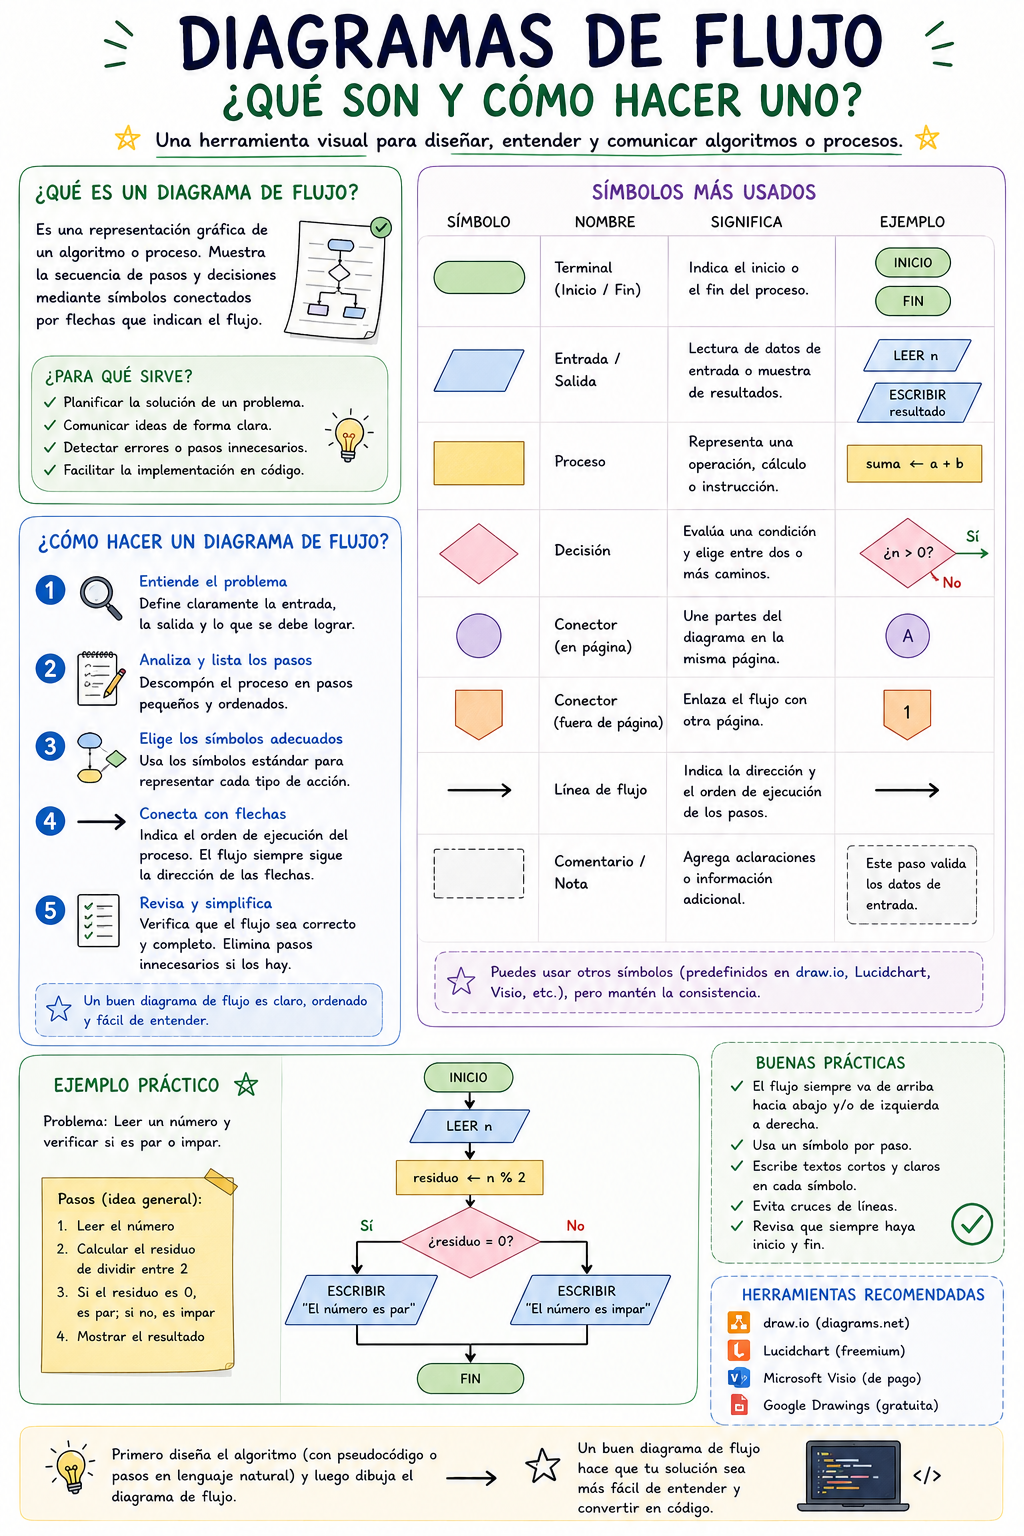
\includegraphics[keepaspectratio]{figures/diagramaflujo_overview.png}}

}

\caption{Imagen creada con ChatGPT.}

\end{figure}%

\section{\texorpdfstring{\textbf{Actividad en equipo: Instrucciones para
los Estudiantes
📝}}{Actividad en equipo: Instrucciones para los Estudiantes 📝}}\label{actividad-en-equipo-instrucciones-para-los-estudiantes}

En equipos de \textbf{3 estudiantes} van a analizar un problema
cotidiano y lo van a documentar en lenguaje natural, pseudocódigo y
diagrama de flujo. La entrega \textbf{será en hoja a mano}, y de manera
opcional podrán utilizar colores para resaltar y organizar la
información. Sube una foto en
la\href{https://classroom.google.com/c/ODcwNTg4NjExNzQ5/a/ODc1MjcyNDQwNjk0/details}{tarea
asiganda en Google classroom}.

\textbf{\hfill\break
Opciones sugeridas:}

\begin{enumerate}
\def\labelenumi{\arabic{enumi}.}
\tightlist
\item
  🍕 \textbf{Pedir comida a domicilio}

  \begin{itemize}
  \tightlist
  \item
    Desde entrar al sitio web hasta recibir la comida
  \end{itemize}
\item
  🚗 \textbf{Estacionar un auto en un estacionamiento}

  \begin{itemize}
  \tightlist
  \item
    Desde que llegas hasta que estacionas correctamente
  \end{itemize}
\item
  📚 \textbf{Buscar y reservar un libro en la biblioteca}

  \begin{itemize}
  \tightlist
  \item
    Desde que entras hasta que lo tienes en tus manos
  \end{itemize}
\item
  💳 \textbf{Retirar dinero de un cajero automático}

  \begin{itemize}
  \tightlist
  \item
    Desde que insertas la tarjeta hasta que obtienes el dinero
  \end{itemize}
\item
  🧺 \textbf{Lavar ropa en una lavadora}

  \begin{itemize}
  \tightlist
  \item
    Desde que separas la ropa hasta que está lista para secar
  \end{itemize}
\item
  🎮 \textbf{Jugar un videojuego desde el inicio}

  \begin{itemize}
  \tightlist
  \item
    Desde que enciendes la consola hasta que empiezas a jugar
  \end{itemize}
\item
  📱 \textbf{Descargar una aplicación en tu teléfono}

  \begin{itemize}
  \tightlist
  \item
    Desde que abres la tienda de aplicaciones hasta que la usas
  \end{itemize}
\item
  🎬 \textbf{Ver una película en una plataforma de streaming}

  \begin{itemize}
  \tightlist
  \item
    Desde que abres la aplicación hasta que la película está
    reproduciéndose
  \end{itemize}
\item
  ✈️ \textbf{Comprar un boleto de avión en línea}

  \begin{itemize}
  \tightlist
  \item
    Desde que buscas el vuelo hasta que recibes la confirmación
  \end{itemize}
\item
  🏥 \textbf{Agendar una cita médica por teléfono}

  \begin{itemize}
  \tightlist
  \item
    Desde que llamas hasta que tienes la cita confirmada
  \end{itemize}
\end{enumerate}

\subsection{\texorpdfstring{\textbf{Paso a
Paso:}}{Paso a Paso:}}\label{paso-a-paso}

\begin{enumerate}
\def\labelenumi{\arabic{enumi}.}
\tightlist
\item
  \textbf{Escribe el problema} en lenguaje natural.
\item
  Escribe el \textbf{objetivo} del programa.
\item
  \textbf{Identifica los pasos principales} que debe seguir el
  algoritmo.
\item
  \textbf{Escribe el pseudocódigo} con estructura clara y lógica.
\item
  \textbf{Dibuja el diagrama de flujo} usando los símbolos correctos:

  \begin{itemize}
  \tightlist
  \item
    Óvalo: Inicio/Fin
  \item
    Rectángulo: Proceso
  \item
    Rombo: Decisión
  \item
    Paralelogramo: Entrada/Salida
  \item
    Flechas: Flujo
  \end{itemize}
\item
  \textbf{Verifica la coherencia} entre los tres elementos.
\item
  \textbf{Revisa casos especiales} (errores, valores límite).
\item
  Prepárate para explicar tu ejemplo en \textbf{5 minutos por equipo}.
\end{enumerate}

\begin{figure}[H]

{\centering \pandocbounded{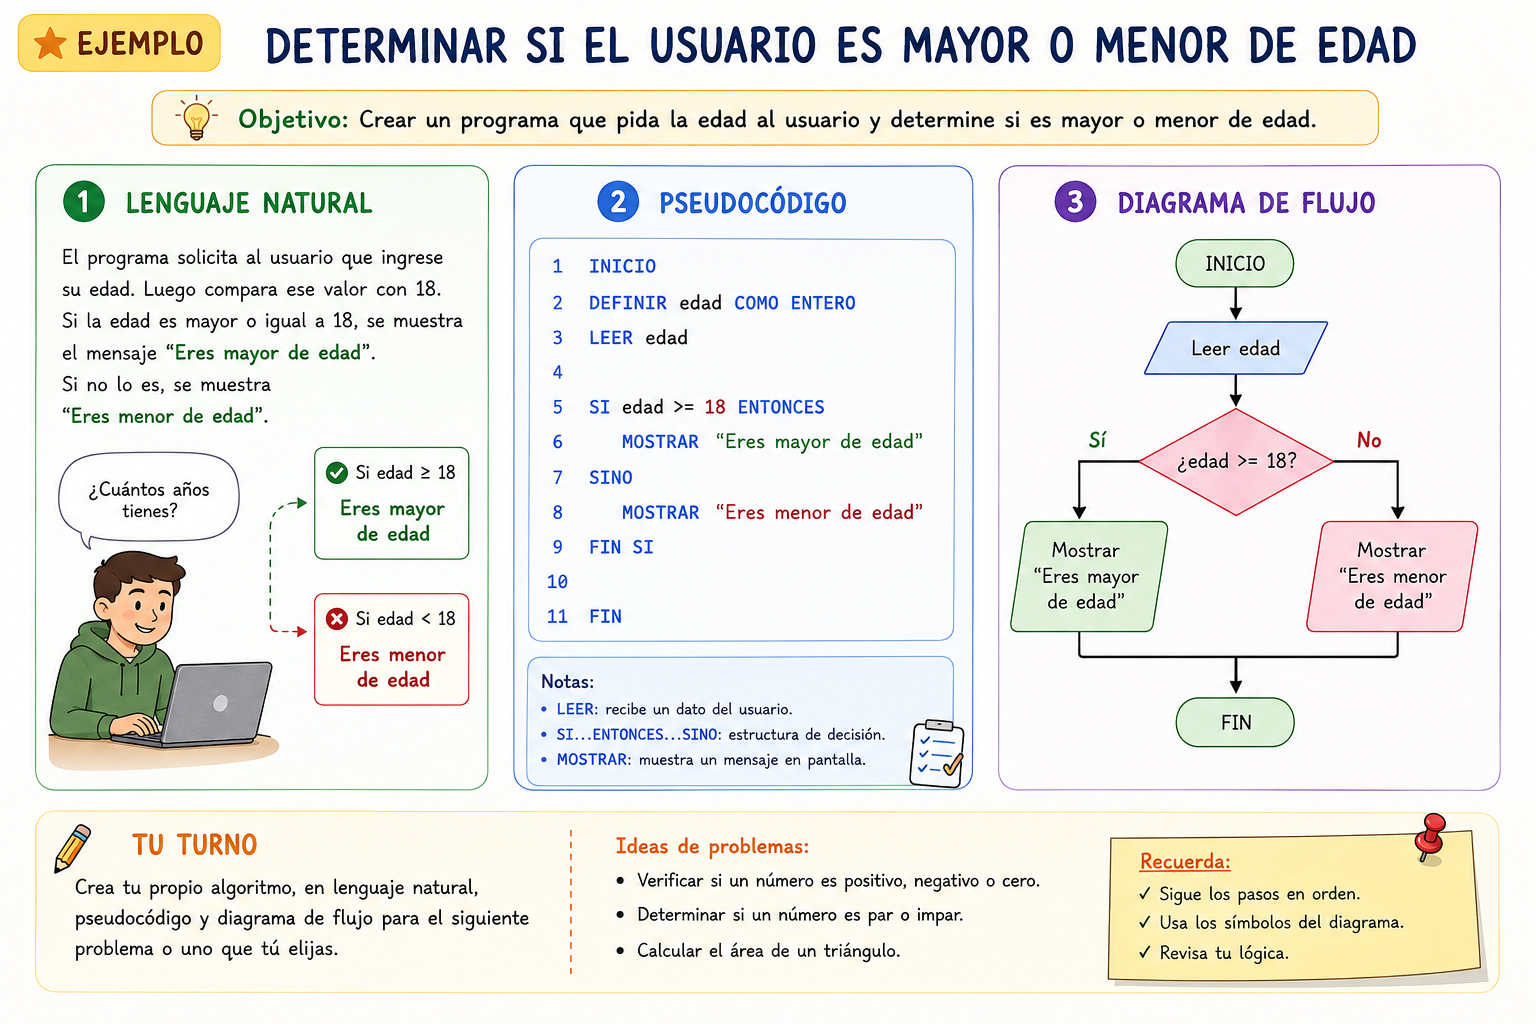
\includegraphics[keepaspectratio]{figures/actividad1_equipo.png}}

}

\caption{Imagen creada con el ejemplo de mayor de edad con ChatGPT.}

\end{figure}%

\part{\textbf{Sección 2} - Instalación de programas}

\chapter{\texorpdfstring{📌 \textbf{To do list -} Instalación de
programas}{📌 To do list - Instalación de programas}}\label{to-do-list---instalaciuxf3n-de-programas}

\begin{figure}[H]

{\centering \pandocbounded{
\includegraphics[keepaspectratio]{figures/fustracion.png}}

}

\caption{Imagen creada con ChatGPT.}

\end{figure}%

El día de hoy nos enfocaremos en la instalación de estos programas, para
ello debes seguir las instrucciones que te he dado:

\begin{tcolorbox}[enhanced jigsaw, arc=.35mm, bottomrule=.15mm, breakable, colback=white, colframe=quarto-callout-tip-color-frame, left=2mm, leftrule=.75mm, opacityback=0, rightrule=.15mm, toprule=.15mm]

Descargar e instalar:

\begin{itemize}
\tightlist
\item[$\square$]
  Git y Bash
\item[$\square$]
  R y Rstudio
\item[$\square$]
  Rtools (Windows) o Xcode (Mac)
\item[$\square$]
  Introducción a R (aquí los veo)
\item[$\square$]
  Python
\item[$\square$]
  Integración de Python en Rstudio con reticulate
\item[$\square$]
  Integración de Bash en Rstudio
\end{itemize}

\end{tcolorbox}

\section{¡ Información importante sobre los equipos
!}\label{informaciuxf3n-importante-sobre-los-equipos-1}

\begin{tcolorbox}[enhanced jigsaw, arc=.35mm, bottomrule=.15mm, bottomtitle=1mm, breakable, colback=white, colbacktitle=quarto-callout-important-color!10!white, colframe=quarto-callout-important-color-frame, coltitle=black, left=2mm, leftrule=.75mm, opacityback=0, opacitybacktitle=0.6, rightrule=.15mm, title=\textcolor{quarto-callout-important-color}{\faExclamation}\hspace{0.5em}{Importante}, titlerule=0mm, toprule=.15mm, toptitle=1mm]

\begin{itemize}
\item
  {\textbf{Asignación de equipos}}

  \begin{itemize}
  \tightlist
  \item
    Deberás trabajar en la \textbf{misma computadora durante todo el
    semestre}.
  \item
    Recuerda que, al finalizar el tiempo de uso, todo lo que hayas
    instalado o guardado en la máquina se \textbf{reinicia y se borra
    automáticamente}.
  \end{itemize}
\item
  {\textbf{Uso de cuentas personales}}

  \begin{itemize}
  \tightlist
  \item
    No debes \textbf{iniciar sesión con tus cuentas personales} en los
    navegadores de las computadoras institucionales.
  \item
    Evita dejar cuentas abiertas, ya que podrían quedar guardadas y otra
    persona podría hacer \textbf{mal uso de ellas}.
  \end{itemize}
\end{itemize}

\pandocbounded{\includegraphics[keepaspectratio]{figures/gif_minionAlert.gif}}

\end{tcolorbox}

\chapter{Instalación de Git y Bash}\label{descarga-Bash}

\begin{quote}
\textbf{Fecha:} 08 de septiembre, 2026
\end{quote}

Para participar en este taller necesitas acceso al siguiente software y
acceso a un navegador como chrome o firefox.

\section{Windows - Git Bash}\label{windows---git-bash}

\textbf{Nota:} Para obtener más detalles sobre cómo instalar y
configurar Git Bash, puedes ver este video tutorial:
\href{https://www.youtube.com/watch?v=t2-l3WvWvqg}{Cómo instalar Git en
Windows 11 (Actualizado 2025)}.

\begin{enumerate}
\def\labelenumi{\arabic{enumi}.}
\item
  Descarga el instalador de \href{https://gitforwindows.org/}{Git para
  Windows}.
\item
  Ejecuta el instalador y sigue los siguientes pasos:

  \begin{itemize}
  \item
    Haz clic en \textbf{``Next'' cuatro veces} (dos veces si ya has
    instalado Git previamente). No necesitas cambiar nada en las
    pantallas de Información, ubicación, componentes y menú de inicio.
  \item
    En el menú desplegable \textbf{``Choosing the default editor used by
    Git'', selecciona ``Use the Nano editor by default''} (NOTA:
    necesitarás desplazarte hacia arriba para encontrarlo) y haz clic en
    ``Next''.
  \item
    En la página que dice \textbf{``Adjusting the name of the initial
    branch in new repositories'', asegúrate de que ``Let Git decide''}
    esté seleccionado. Esto garantizará el nivel más alto de
    compatibilidad para nuestras lecciones.
  \item
    Asegúrate de que esté seleccionada la opción \textbf{``Git from the
    command line and also from 3rd-party software'' y haz clic en
    ``Next''.} (Si no haces esto, Git Bash no funcionará correctamente,
    lo que te obligará a eliminar la instalación de Git Bash, volver a
    ejecutar el instalador y seleccionar la opción ``\textbf{Git from
    the command line and also from 3rd-party software'').}
  \item
    Selecciona \textbf{``Use bundled OpenSSH''}.
  \item
    Asegúrate de que \textbf{``Use the native Windows Secure Channel
    Library'' esté seleccionada y haz clic en ``Next''}.
  \item
    Asegúrate de que \textbf{``Checkout Windows-style, commit Unix-style
    line endings'' esté seleccionada y haz clic en ``Next''.}
  \item
    Asegúrate de que \textbf{``Use Windows' default console window''}
    esté seleccionada y haz clic en ``Next''.
  \item
    Asegúrate de que \textbf{``Default (fast-forward or merge)''} esté
    seleccionada y haz clic en ``Next''.
  \item
    Asegúrate de que \textbf{``Git Credential Manager''} esté
    seleccionada y haz clic en ``Next''.
  \item
    Asegúrate de que \textbf{``Enable file system caching''} esté
    seleccionada y haz clic en ``Next''.
  \item
    Haz clic en \textbf{``Install''}.
  \item
    Haz clic en \textbf{``Finish'' o ``Next''}.
  \end{itemize}
\item
  Si tu variable de entorno \textbf{``HOME''} no está configurada (o no
  sabes qué es):
\end{enumerate}

\begin{itemize}
\tightlist
\item
  Abre el símbolo del sistema (abre el menú de inicio, luego escribe
  \texttt{cmd} y presiona \textbf{Enter}).
\item
  Escribe la siguiente línea exactamente como se muestra en la ventana
  del símbolo del sistema.
\end{itemize}

\begin{Shaded}
\begin{Highlighting}[]
\ExtensionTok{setx}\NormalTok{ HOME }\StringTok{"\%USERPROFILE\%"}
\end{Highlighting}
\end{Shaded}

\begin{itemize}
\tightlist
\item
  Presiona Enter, deberías ver ``SUCCESS: Specified value was saved''.
\item
  Cierra el símbolo del sistema escribiendo ``exit'' y presionando
  Enter.
\end{itemize}

Esto te proporcionará tanto Git como Bash en el programa \textbf{Git
Bash}.

\section{macOS - Git}\label{macos---git}

En macOS, el shell por defecto en la mayoría de las versiones es
\textbf{\texttt{Bash}}, por lo que no es necesario instalarlo Puedes
acceder a Bash desde la aplicación \textbf{Terminal}, ubicada en
\textbf{/Applications/Utilities/}\\

\textbf{Nota:} Para obtener más detalles sobre cómo instalar y
configurar Git Bash, puedes ver este video tutorial:
\href{https://www.youtube.com/watch?v=kdM9YOX2hZ0}{Instalar Git
fácilmente en MacOS 2025}\\

En el sitio oficial de \href{https://git-scm.com/install/mac}{git}
existen varias opciones para la instalación en macOS, en este caso se
llevará a cabo a través de \href{https://brew.sh/}{\textbf{Homebrew}}.

\begin{enumerate}
\def\labelenumi{\arabic{enumi}.}
\item
  Instalar Homebrew (en caso de que no esté instalado)

  \begin{itemize}
  \item
    Busca y abre la aplicación de la terminal en tu computadora
  \item
    Copia y pega el siguiente código en la terminal y presiona
    \textbf{Enter}

\begin{verbatim}
/bin/bash -c "$(curl -fsSL https://raw.githubusercontent.com/Homebrew/install/HEAD/install.sh)"
\end{verbatim}
  \item
    Presiona \textbf{Enter} para comenzar la instalación
  \item
    Una vez que acabe la instalación, verifica que la instalación se
    haya llevado a cabo correctamente con el siguiente código:

\begin{verbatim}
brew --version
\end{verbatim}

    Después de presionar \textbf{Enter} aparecerá la última versión de
    \textbf{Homebrew} \texttt{Homebrew\ 4.5.7}
  \end{itemize}
\item
  Una vez instalado \textbf{Homebrew} copia y pega el siguiente código
  en la terminal

\begin{verbatim}
brew install git
\end{verbatim}

  Presiona \textbf{Enter}
\end{enumerate}

Se recomienda mantener la Terminal anclada en el Dock para facilitar su
uso durante el taller

\section{Linux - Git}\label{linux---git}

La mayoría de las distribuciones de \textbf{Linux} incluyen
\textbf{Bash} como shell predeterminado y \textbf{Git} instalado por
defecto.\\

Si tu sistema es diferente, abre una terminal y ejecuta el comando:

\begin{verbatim}
bash
\end{verbatim}

\begin{figure}[H]

{\centering \pandocbounded{
\includegraphics[keepaspectratio]{figures/colina_gitbash.png}}

}

\caption{Imagen creada con ChatGPT.}

\end{figure}%

\chapter{Instalación de R, RStudio y Rtools/XCode}\label{descarga-R}

\begin{quote}
\textbf{Fecha:} 08 de septiembre, 2026
\end{quote}

Para participar en este taller necesitas acceso a los siguientes
software y acceso a un navegador como chrome o firefox.

\begin{tcolorbox}[enhanced jigsaw, arc=.35mm, bottomrule=.15mm, bottomtitle=1mm, breakable, colback=white, colbacktitle=quarto-callout-important-color!10!white, colframe=quarto-callout-important-color-frame, coltitle=black, left=2mm, leftrule=.75mm, opacityback=0, opacitybacktitle=0.6, rightrule=.15mm, title=\textcolor{quarto-callout-important-color}{\faExclamation}\hspace{0.5em}{Orden de instalación}, titlerule=0mm, toprule=.15mm, toptitle=1mm]

El orden importa, primero instala R -\textgreater{} Rstudio
-\textgreater{} Rtools.

Nuncia instales primero Rstudio antes que R

\end{tcolorbox}

\section{Windows - R}\label{windows---r}

\textbf{Nota:} Para obtener más detalles sobre cómo instalar y
configurar R y Rstudio, puedes ver este video tutorial:
\href{https://www.youtube.com/watch?v=H9EBlFDGG4k}{Cómo instalar R y
RStudio en Windows 11}.

\begin{enumerate}
\def\labelenumi{\arabic{enumi}.}
\item
  Entra a la siguiente \href{https://cloud.r-project.org/}{página}
\item
  Haz click en \ul{\textbf{Download R for Windows}}
\item
  Haz click en \ul{\textbf{install R for the first time}}
\item
  Haz click en \ul{\textbf{Download R-4.5.2 for Windows}}
\item
  Ejecuta el instalador y sigue los siguientes pasos:

  \begin{itemize}
  \item
    Selecciona el lenguaje de preferencia durante el proceso y haz click
    en ``\textbf{OK}''
  \item
    Haz clic en ``\textbf{Next}''
  \item
    Haz clic en ``\textbf{Next}'' (Si deseas cambiar el sitio de
    instalación, haz clic en ``\textbf{Browse}'' y selecciona tu carpeta
    deseada).
  \item
    Haz click en ``\textbf{Next}'' en las siguientes cuatro ventanas
  \item
    Espera unos minutos a que finalice la instalación y haz click en
    ``\textbf{Finish}''
  \end{itemize}
\end{enumerate}

\section{Windows - Rstudio}\label{windows---rstudio}

\begin{enumerate}
\def\labelenumi{\arabic{enumi}.}
\tightlist
\item
  Entra en la siguiente
  \href{https://posit.co/download/rstudio-desktop/\#download}{página}
\item
  Haz click en \textbf{Download RStudio Desktop for Windows}
\item
  Ejecuta el instalador y sigue los siguientes pasos:

  \begin{itemize}
  \tightlist
  \item
    Haz clic en ``\textbf{Next}''
  \item
    Haz clic en ``\textbf{Next}'' (Si deseas cambiar el sitio de
    instalación, haz clic en ``\textbf{Browse}'' y selecciona tu carpeta
    deseada).
  \item
    Haz clic en ``\textbf{Install}'' y espera unos minutos a que acabe
    el proceso
  \item
    Haz clic en ``\textbf{Finish}''
  \end{itemize}
\item
  Abre la aplicación de RStudio
\item
  Haz clic en ``\textbf{OK}''
\end{enumerate}

\section{macOS - R}\label{macos---r}

\textbf{Nota:} Para obtener más detalles sobre cómo instalar y
configurar Git Bash, puedes ver este video tutorial:
\href{https://www.youtube.com/watch?v=_k8seoE6b-E}{Cómo instalar R y R
Studio en MacOS}

\begin{enumerate}
\def\labelenumi{\arabic{enumi}.}
\item
  Entra a la siguiente \href{https://cloud.r-project.org/}{página}
\item
  Haz click en \ul{\textbf{Download R for macOS}}
\item
  Existen dos versiones de R que dependen del procesador de tu
  computadora. Para ver la versión de tu procesador, haz click en el
  ícono de apple en la parte superior izquierda de tu pantalla y
  selecciona ``acerca de esta mac''. En la ventana emergente, la versión
  de tu procesador aparecerá junto a la palabra ``Chip'', por ejemplo:
  \textbf{Chip Apple M1 Pro}

  \begin{itemize}
  \item
    Para Mac con \textbf{Apple Silicon} (M1,2,\ldots) haz clic en
    \ul{R-4.5.2-arm64.pkg}
  \item
    Para Mac con procesador \textbf{Intel} haz clic en
    \ul{R-4.5.2-x86\_64.pkg}
  \end{itemize}
\item
  Ejecuta el instalador y sigue los siguientes pasos:

  \begin{itemize}
  \item
    Haz clic en ``\textbf{Continuar}'' tres veces
  \item
    Haz clic en ``\textbf{De acuerdo}''
  \item
    Haz click en ``\textbf{Instalar}''
  \item
    Espera unos minutos a que finalice la instalación y haz click en
    ``\textbf{Cerrar}''
  \end{itemize}
\end{enumerate}

\section{macOS- Rstudio}\label{macos--rstudio}

\begin{enumerate}
\def\labelenumi{\arabic{enumi}.}
\tightlist
\item
  Entra en la siguiente
  \href{https://posit.co/download/rstudio-desktop/\#download}{página}
\item
  Haz click en \textbf{Download RStudio Desktop for macOS 13+}

  \begin{itemize}
  \tightlist
  \item
    Para ver la versión de tu procesador, haz click en el ícono de apple
    en la parte superior izquierda de tu pantalla y selecciona ``acerca
    de esta mac''. En la ventana emergente, la versión de tu sistema
    operativo aparecerá junto a la palabra ``macOS'', por ejemplo:
    \textbf{macOS Sequola} 15.1.1.
  \item
    Si la versión de tu sistema operativo está por debajo de la versión
    13, haz clic en \ul{\textbf{download a previous version}}.
  \end{itemize}
\item
  Ejecuta el instalador
\item
  Arrastra el ícono de RStudio a la carpeta de aplicaciones y espera a
  que finalice la instalación
\end{enumerate}

\section{Linux - R}\label{linux---r}

\begin{enumerate}
\def\labelenumi{\arabic{enumi}.}
\item
  Entra a la siguiente \href{https://cloud.r-project.org/}{página}
\item
  Junto a \ul{\textbf{Download R for Linux}} existen tres opciones,
  selecciona la que se ajusta a tu distribución de Linux

  \begin{itemize}
  \item
    \ul{\textbf{Debian}}
  \item
    \ul{\textbf{Fedora/Redhat}}
  \item
    \ul{\textbf{Ubuntu}}
  \end{itemize}
\item
  Para instalar Linux en \textbf{Debian} y ejecuta las siguientes líneas
  de código (presiona \textbf{Enter} después de cada línea de código):

  \begin{itemize}
  \item
    \texttt{sudo\ apt\ update}
  \item
    \texttt{sudo\ apt\ install\ r-base\ r-base-dev}
  \end{itemize}
\item
  Para instalar Linux en \textbf{Fedora/Redhat} y ejecuta la siguiente
  línea de código:

  \begin{itemize}
  \item
    \texttt{sudo\ dnf\ install\ R}
  \item
    Presiona \textbf{Enter}
  \end{itemize}
\item
  Para instalar Linux en \textbf{Ubuntu} y ejecuta las siguientes líneas
  de código (presiona \textbf{Enter} después de cada línea de código):

  \begin{itemize}
  \item
    \texttt{sudo\ apt\ update\ -qq}
  \item
    \texttt{sudo\ apt\ install\ -\/-no-install-recommends\ software-properties-common\ dirmngr}
  \item
    \texttt{wget\ -qO-\ https://cloud.r-project.org/bin/linux/ubuntu/marutter\_pubkey.asc\ \textbar{}\ sudo\ tee\ -a\ /etc/apt/trusted.gpg.d/cran\_ubuntu\_key.asc}
  \item
    \texttt{sudo\ add-apt-repository\ "deb\ https://cloud.r-project.org/bin/linux/ubuntu\ \$(lsb\_release\ -cs)-cran40/"}
  \item
    \texttt{sudo\ apt\ install\ -\/-no-install-recommends\ r-base}
  \end{itemize}
\end{enumerate}

\section{Linux - RStudio}\label{linux---rstudio}

\begin{enumerate}
\def\labelenumi{\arabic{enumi}.}
\tightlist
\item
  Entra en la siguiente
  \href{https://posit.co/download/rstudio-desktop/\#download}{página}
\item
  Desliza la página hasta llegar a la tabla de opciones de instalación
\item
  Selecciona tu opción de accuerdo con la distribución y versión de tu
  sistema operativo (\ul{\textbf{Debian, Fedora/Redhat, Ubuntu}}).
\item
  Ejecuta el instalador
\end{enumerate}

\section{Actualizar R - Windows y
MacOS}\label{actualizar-r---windows-y-macos}

Si ya tienes R instalado en tu computadora, asegúrate de tener la
versión más actualizada de R

Existen diferentes formas de actualizar R, la manera más sencilla es a
través de \textbf{Rgui,} la interfaz gráfica que viene con R base, no
con RStudio.

\textbf{Windows y MacOS}:

\begin{enumerate}
\def\labelenumi{\arabic{enumi}.}
\item
  Escribe \textbf{Rgui} en el explorador de archivos/aplicaciones de tu
  computadora para abrir la aplicación de R.
\item
  Para actualizar R necesitamos de la paquetería \textbf{installr}. Para
  instalarla ejecuta el siguiente código:
\end{enumerate}

\begin{verbatim}
-   `install.packages(installr)`
-   Presiona **Enter**
\end{verbatim}

\begin{enumerate}
\def\labelenumi{\arabic{enumi}.}
\setcounter{enumi}{2}
\item
  Carga la paquetería con la función \texttt{library()}

  \begin{itemize}
  \tightlist
  \item
    library\texttt{(installr)}
  \item
    Presiona \textbf{Enter}
  \end{itemize}
\item
  Para revisar si tienes la versión de R más actualizada ejecuta el
  siguiente código:

  \begin{itemize}
  \tightlist
  \item
    \texttt{installr(GUI\ =\ TRUE)}
  \item
    Presiona \textbf{Enter}
  \item
    En la ventana emergente asegúrate de tener seleccionada la opción
    ``R (updateR)'' y haz clic en ``OK''
  \end{itemize}
\item
  Aparecerá otra ventana con información sobre la versión de R que estás
  usando y si existe una versión más reciente.

  \begin{itemize}
  \tightlist
  \item
    Si \textbf{ya tienes la versión más actual}, simplemente haz clic en
    \textbf{``OK''} para cerrar.
  \item
    Si \textbf{hay una versión nueva disponible}, haz clic en
    \textbf{``Yes''} para comenzar la actualización.
  \end{itemize}
\item
  Si durante el proceso aparece una ventana preguntando si deseas copiar
  paquetes o configuraciones anteriores, puedes hacer clic en
  \textbf{``No''} (no es obligatorio copiarlos; puedes reinstalarlos
  después si lo prefieres).
\end{enumerate}

\section{Evitar conflictos para la instalación de paquetes en
R}\label{evitar-conflictos-para-la-instalaciuxf3n-de-paquetes-en-r}

\subsection{Si usamos Windows debemos instalar
Rtools}\label{si-usamos-windows-debemos-instalar-rtools}

En \textbf{Windows} utilizamos \textbf{Rtools} para evitar problemas al
instalar paquetes desde código fuente en RStudio. Selecciona la versión
que se adapta a tu versión de R.

\begin{center}
\pandocbounded{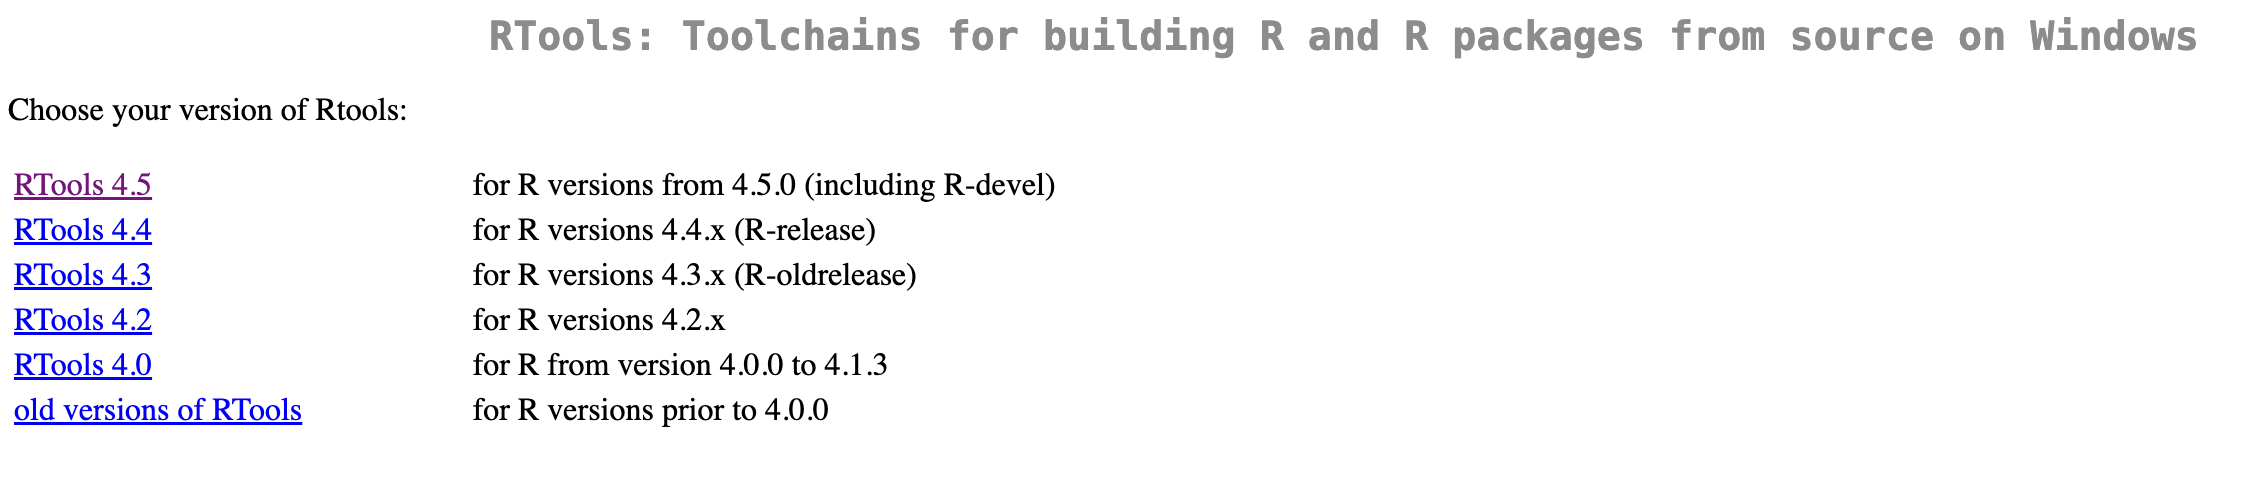
\includegraphics[keepaspectratio]{figures/rtools_windows.png}}
\end{center}

Yo seleccioné la versión Rtools 4.5 y me aparece la siguiente página
web, después di clic en donde aparece el instalador, descargue el
archivo y lo ejecute.

\begin{center}
\pandocbounded{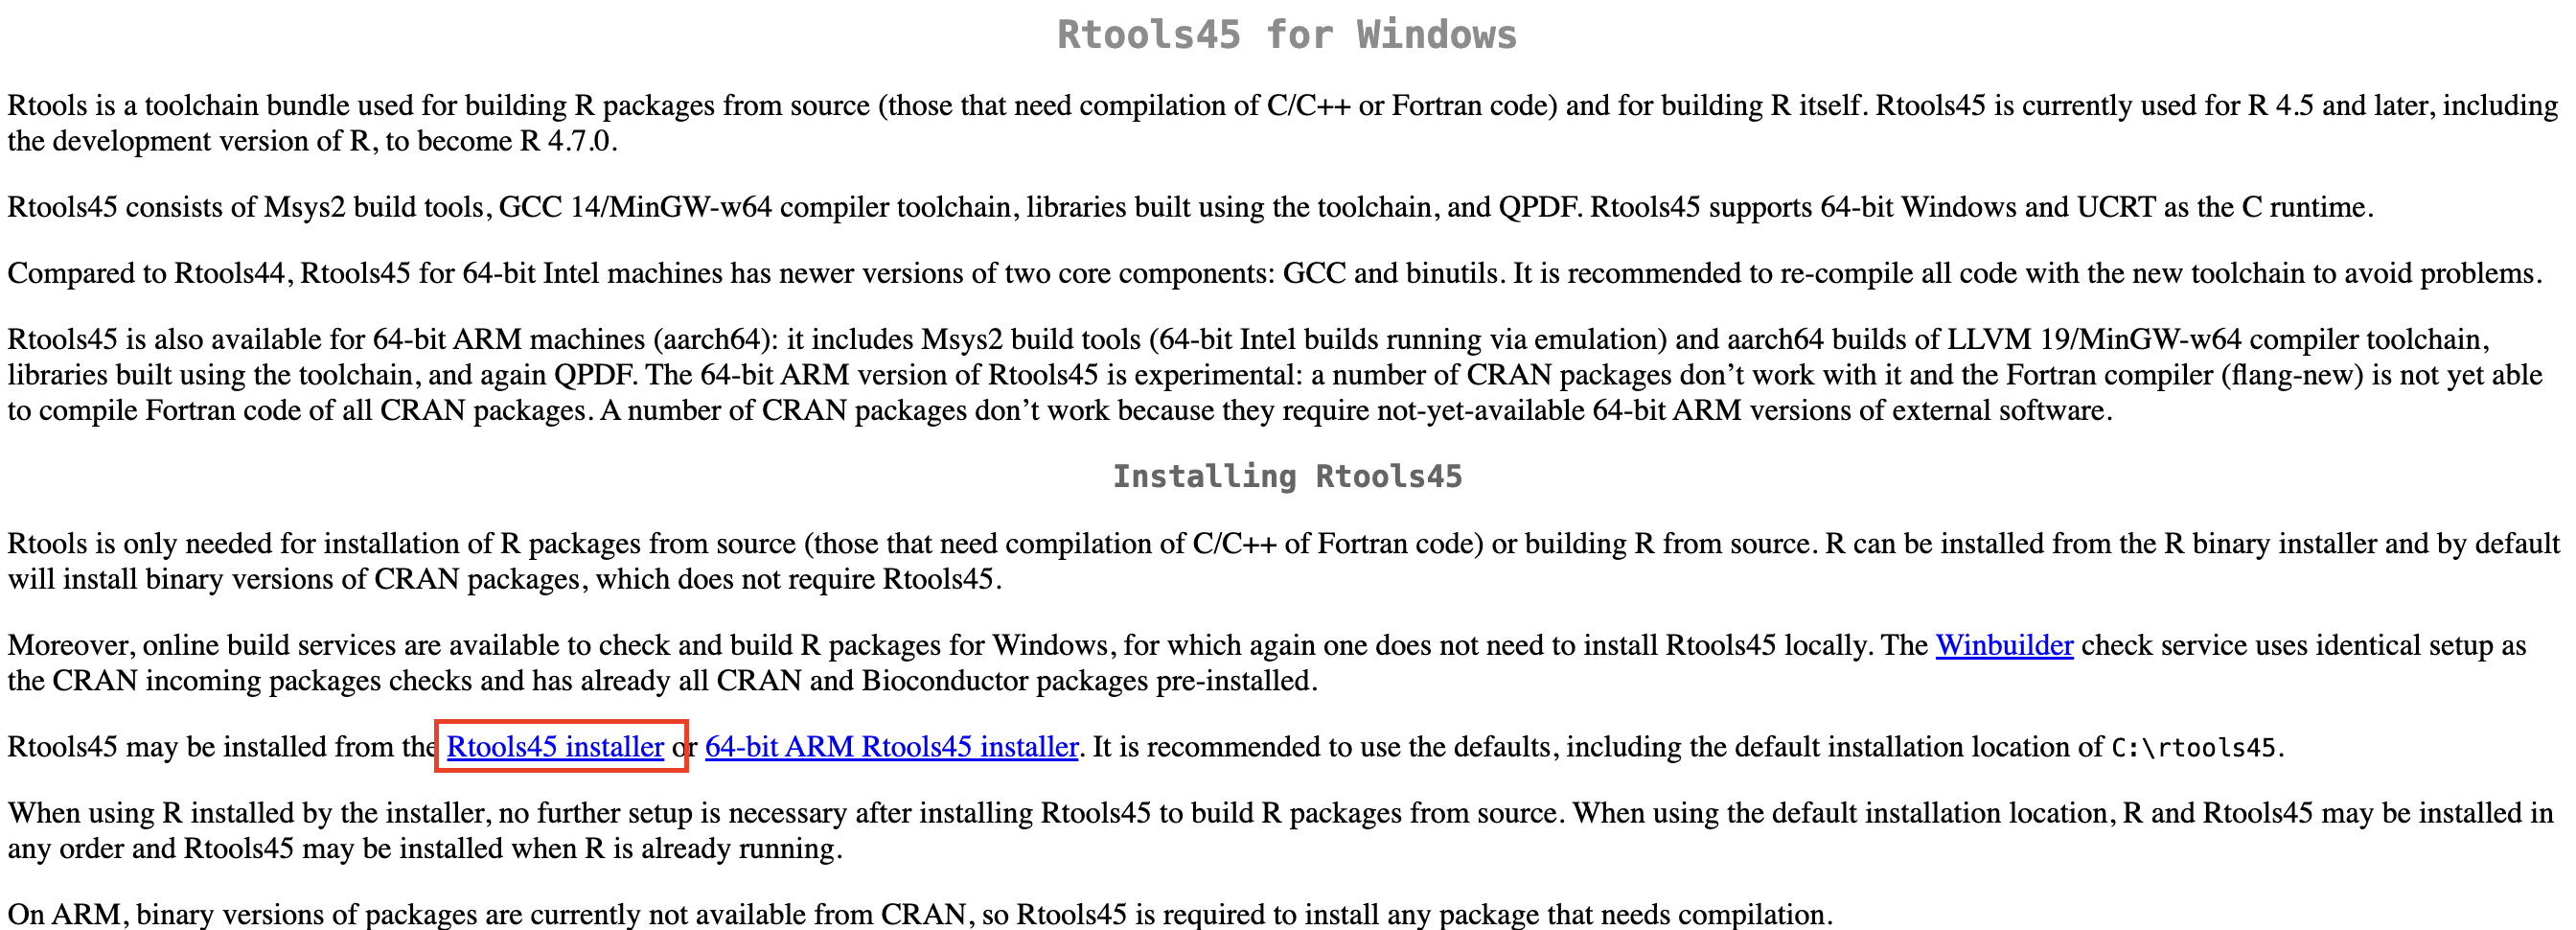
\includegraphics[keepaspectratio]{figures/rtools_installer.png}}
\end{center}

\subsection{Si usamos MacOs debemos instalar
Xcode}\label{si-usamos-macos-debemos-instalar-xcode}

En \textbf{macOS}, no existe un equivalente directo a Rtools. En su
lugar, se emplean las
\href{https://mac.r-project.org/tools/}{\textbf{Xcode Command Line
Tools}} (que incluyen \texttt{clang} y \texttt{make}) junto con
\textbf{GNU Fortran} para compilar paquetes que requieren código en
C/C++ o Fortran.

\pandocbounded{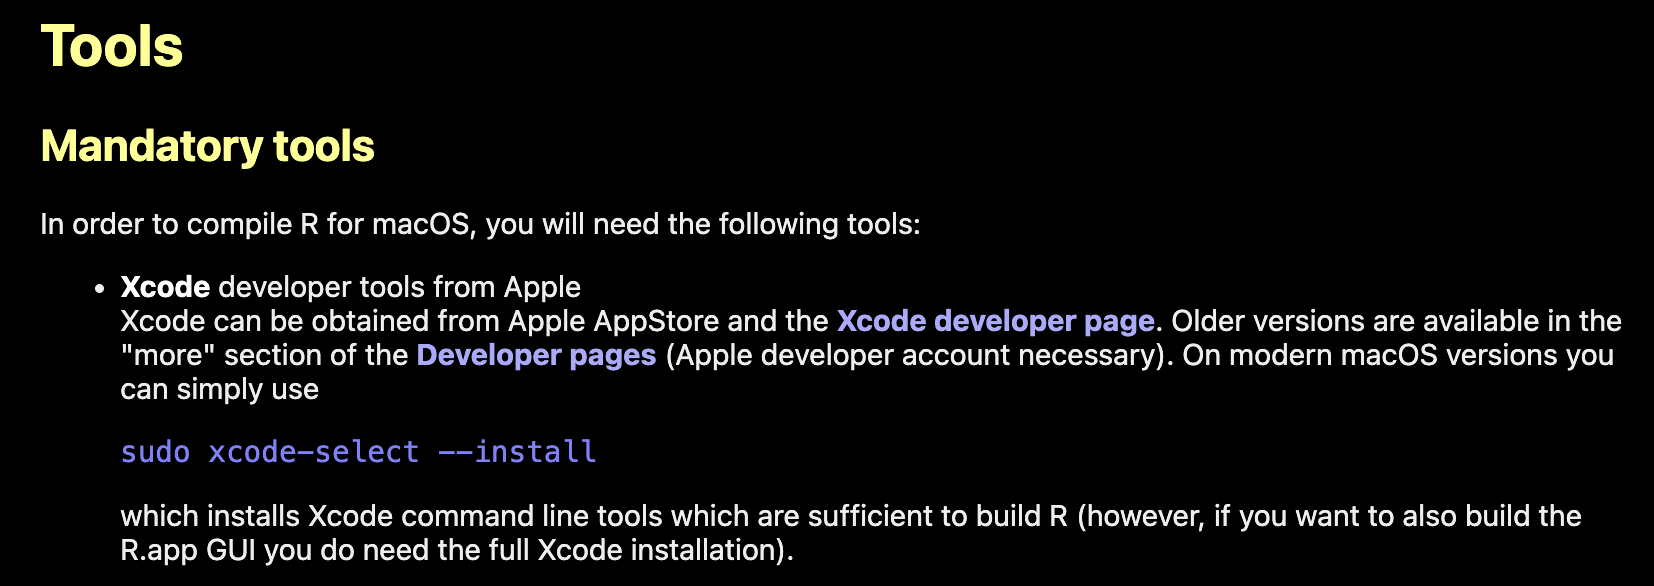
\includegraphics[keepaspectratio]{figures/xcode_mac.png}}

Esto significa que, si trabajan en Mac, deben asegurarse de tener
instaladas estas herramientas para evitar errores al instalar ciertos
paquetes de R. Abre una terminal de Bash y coloca este código:

\begin{Shaded}
\begin{Highlighting}[]
\FunctionTok{sudo}\NormalTok{ xcode{-}select }\AttributeTok{{-}{-}install}
\end{Highlighting}
\end{Shaded}

\begin{figure}[H]

{\centering \pandocbounded{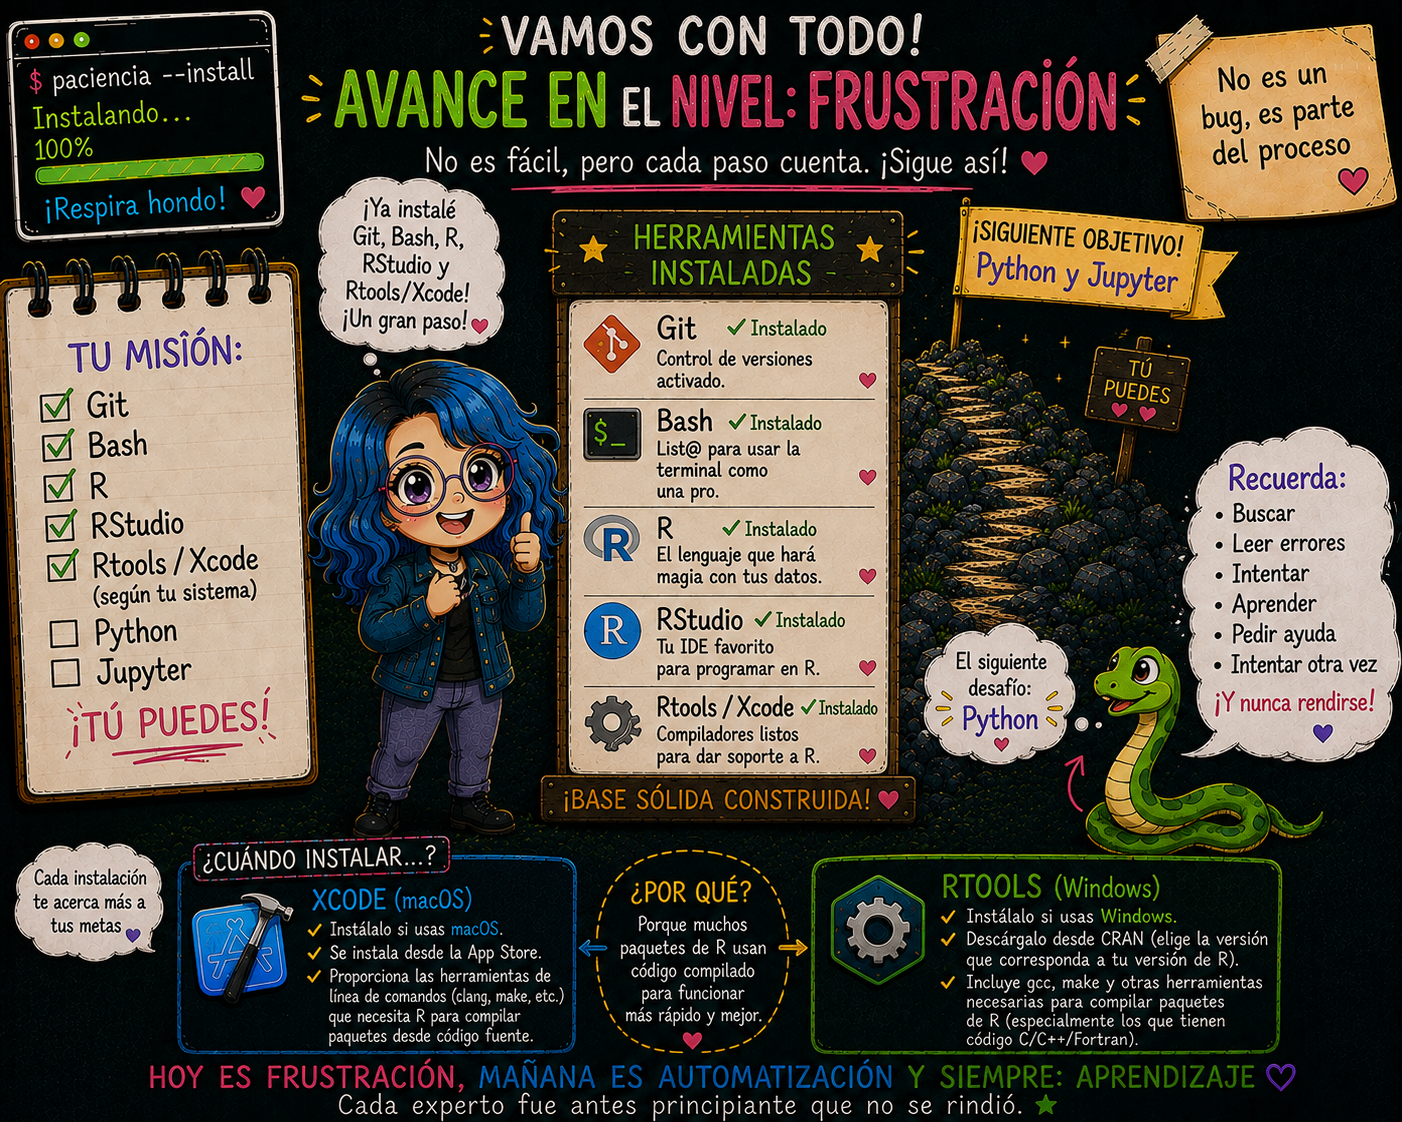
\includegraphics[keepaspectratio]{figures/colina_rinstall.png}}

}

\caption{Imagen creada con ChatGPT.}

\end{figure}%

\chapter{Introducción a R y
Rstudio}\label{introducciuxf3n-a-r-y-rstudio}

\begin{quote}
\textbf{Fecha:} 08 de septiembre, 2026
\end{quote}

\section{¿Qué es R?}\label{quuxe9-es-r}

R es un entorno de desarrollo de software libre y lenguaje de
programación.

\textbf{¿Por qué utilizar R?}

Es ampliamente utilizado para la \emph{computación estadística, gráfica,
y de machine learning}. Ofrece una amplia variedad de \textbf{funciones
estadísticas} (modelos lineales y no lineales, pruebas estadísticas
clásicas, análisis de series de tiempo, clasificación, agrupamiento,
etc.), y para realizar gráficas.

Además, existen numerosas librerías que nos pemiten realizar análisis y
más gráficas, incluyendo para análisis de datos genómicos.

\hfill

\includegraphics[width=2.63542in,height=\textheight,keepaspectratio]{figures/r-logo.png}

\section{¿Cómo instalamos R?}\label{cuxf3mo-instalamos-r}

Para installar R, debemos de entrar a la página de
\href{https://cran.r-project.org/}{CRAN} ``The Comprehensive R Archive
Network''. Al installar R, descargamos también \textasciitilde{} 25
paqueterías/librerías.

\textbf{CRAN} es una red en la que se archivan todas las versiones de R
base, así como todos los paquetes para R que han pasado por un proceso
de revisión riguroso, realizado por el CRAN Team.

\pandocbounded{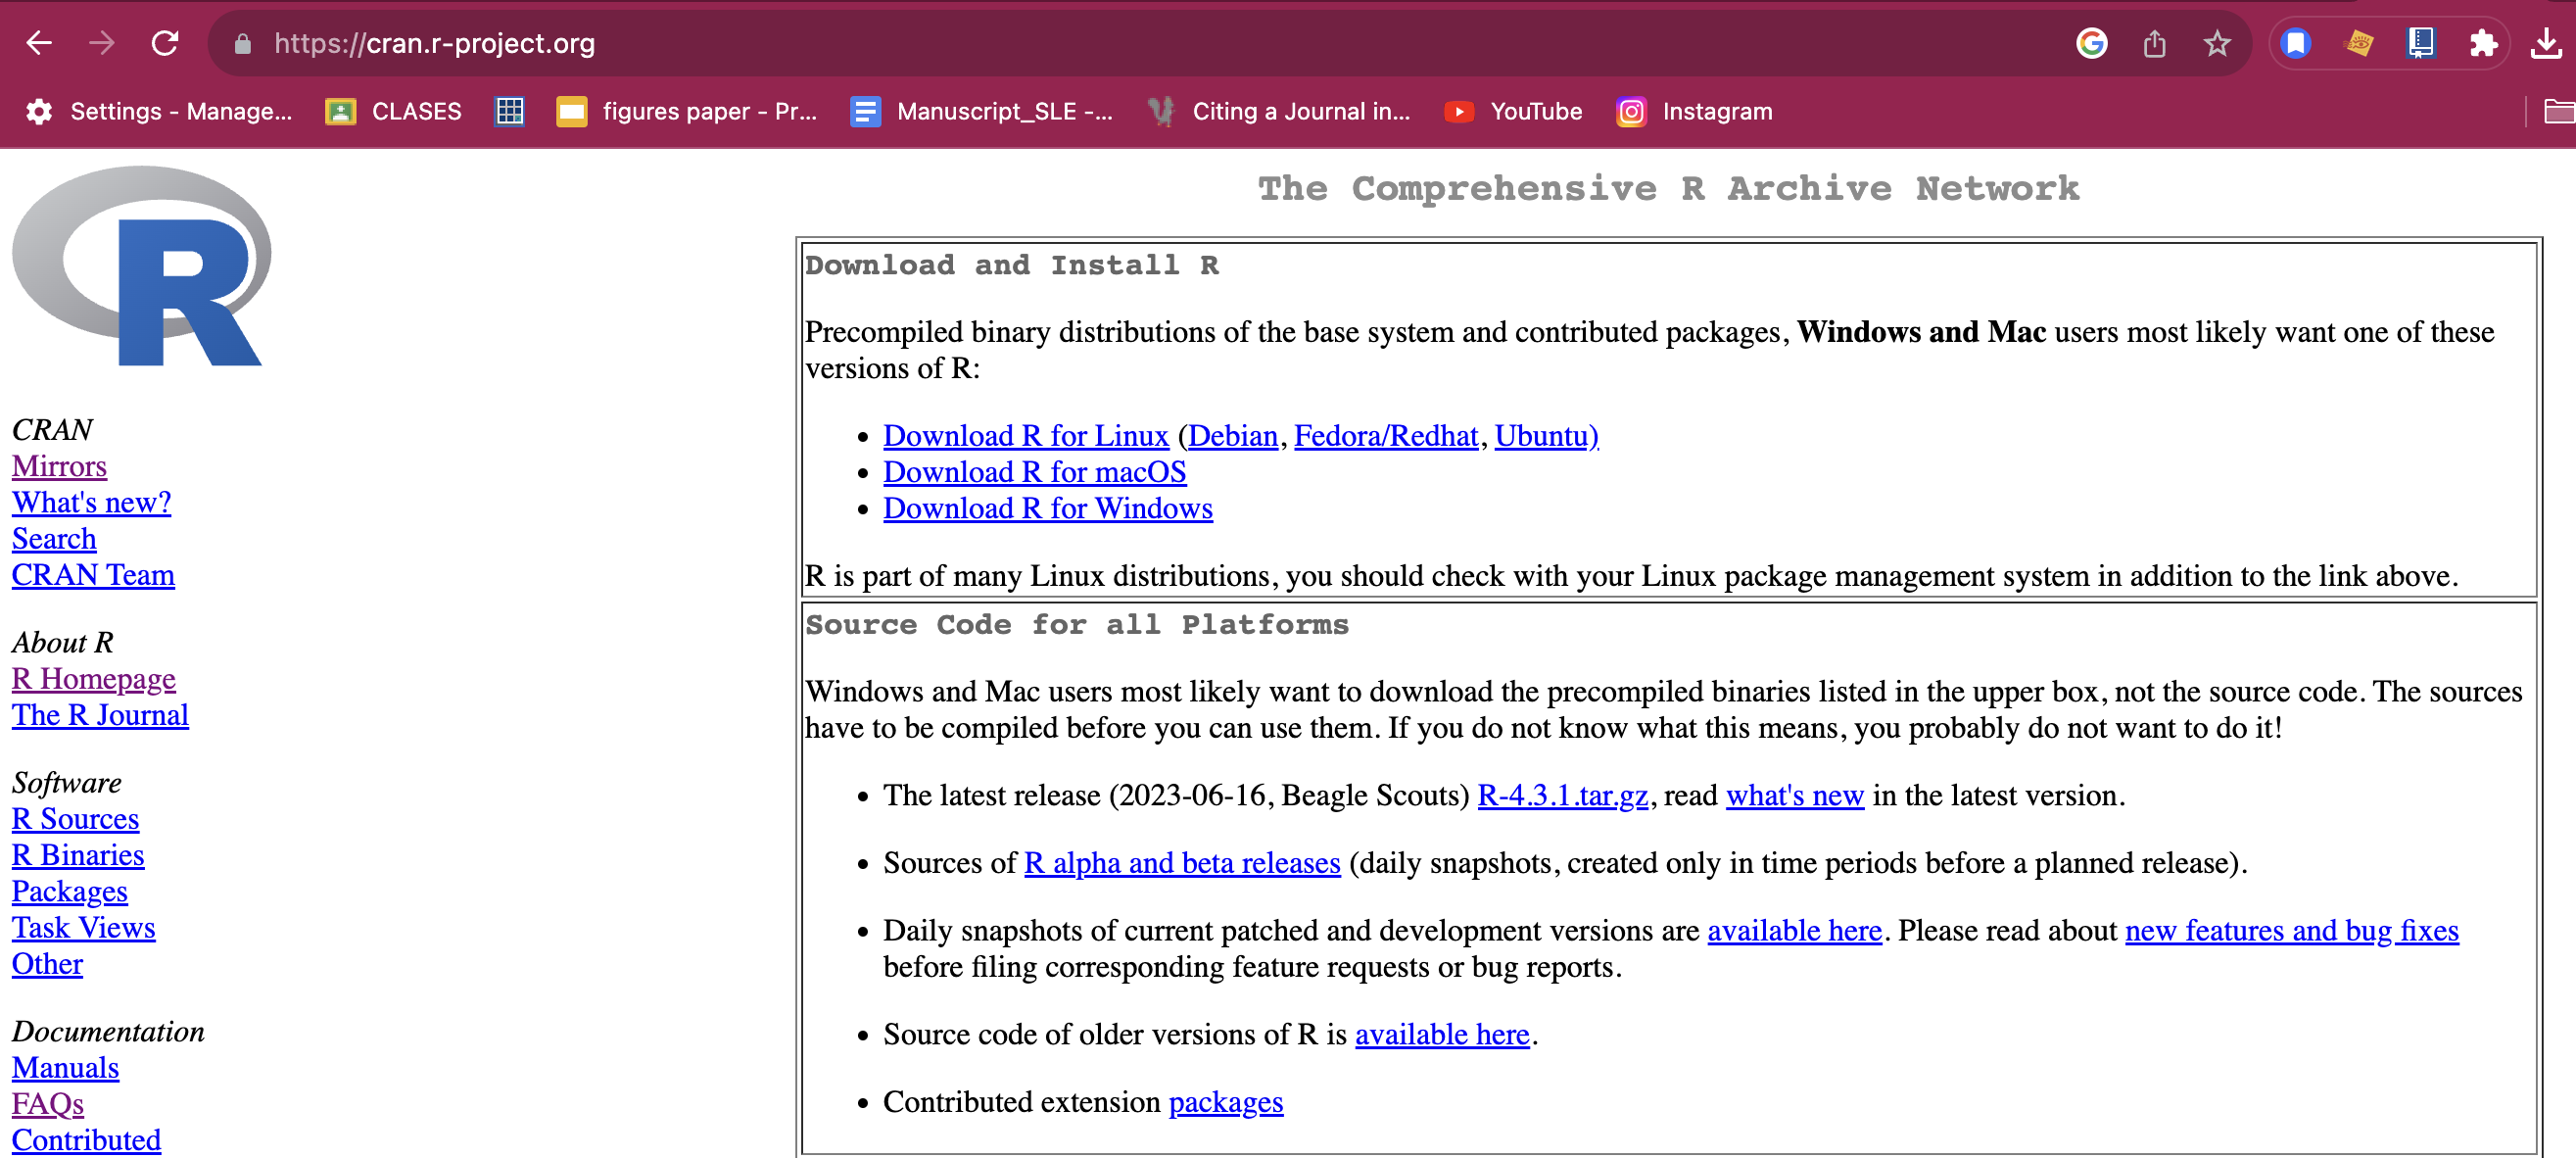
\includegraphics[keepaspectratio]{figures/download-r.png}}

\section{¿Qué es RStudio?}\label{quuxe9-es-rstudio}

RStudio es un \textbf{entorno de desarrollo integrado (IDE)} para R. Un
IDE es una aplicación que ayuda a los programadores a \emph{desarrollar
código de una manera eficiente}. Nos proporciona una interfaz para poder
editar código fuente, herramientas de ambiente, visualización, terminal
y consola.

\textbf{RStudio Desktop} es una aplicación que se utiliza ampliamente
para desarrollar programas en R, pero también podemos accesar al IDE de
RStudio a través con
\href{https://posit.co/download/rstudio-server/}{RStudio Server}, a
través de un navegador web.

\pandocbounded{
\includegraphics[keepaspectratio]{figures/rstudio-logo.png}}

\section{¿Cómo descargamos RStudio?}\label{cuxf3mo-descargamos-rstudio}

Podemos descargar RStudio desde
\href{https://posit.co/download/rstudio-desktop/}{esta página}. Ya
realizamos el paso 1: Install R.

En el paso 2: Install R studio, nos debería detectar el sistema
operativo, descarguemos la versión recomendada en el botón \textbf{azul}
y sigamos las instrucciones de instalación.

\pandocbounded{
\includegraphics[keepaspectratio]{figures/download-rstudio.png}}

\section{Las partes de RStudio}\label{las-partes-de-rstudio}

\begin{figure}[H]

{\centering \pandocbounded{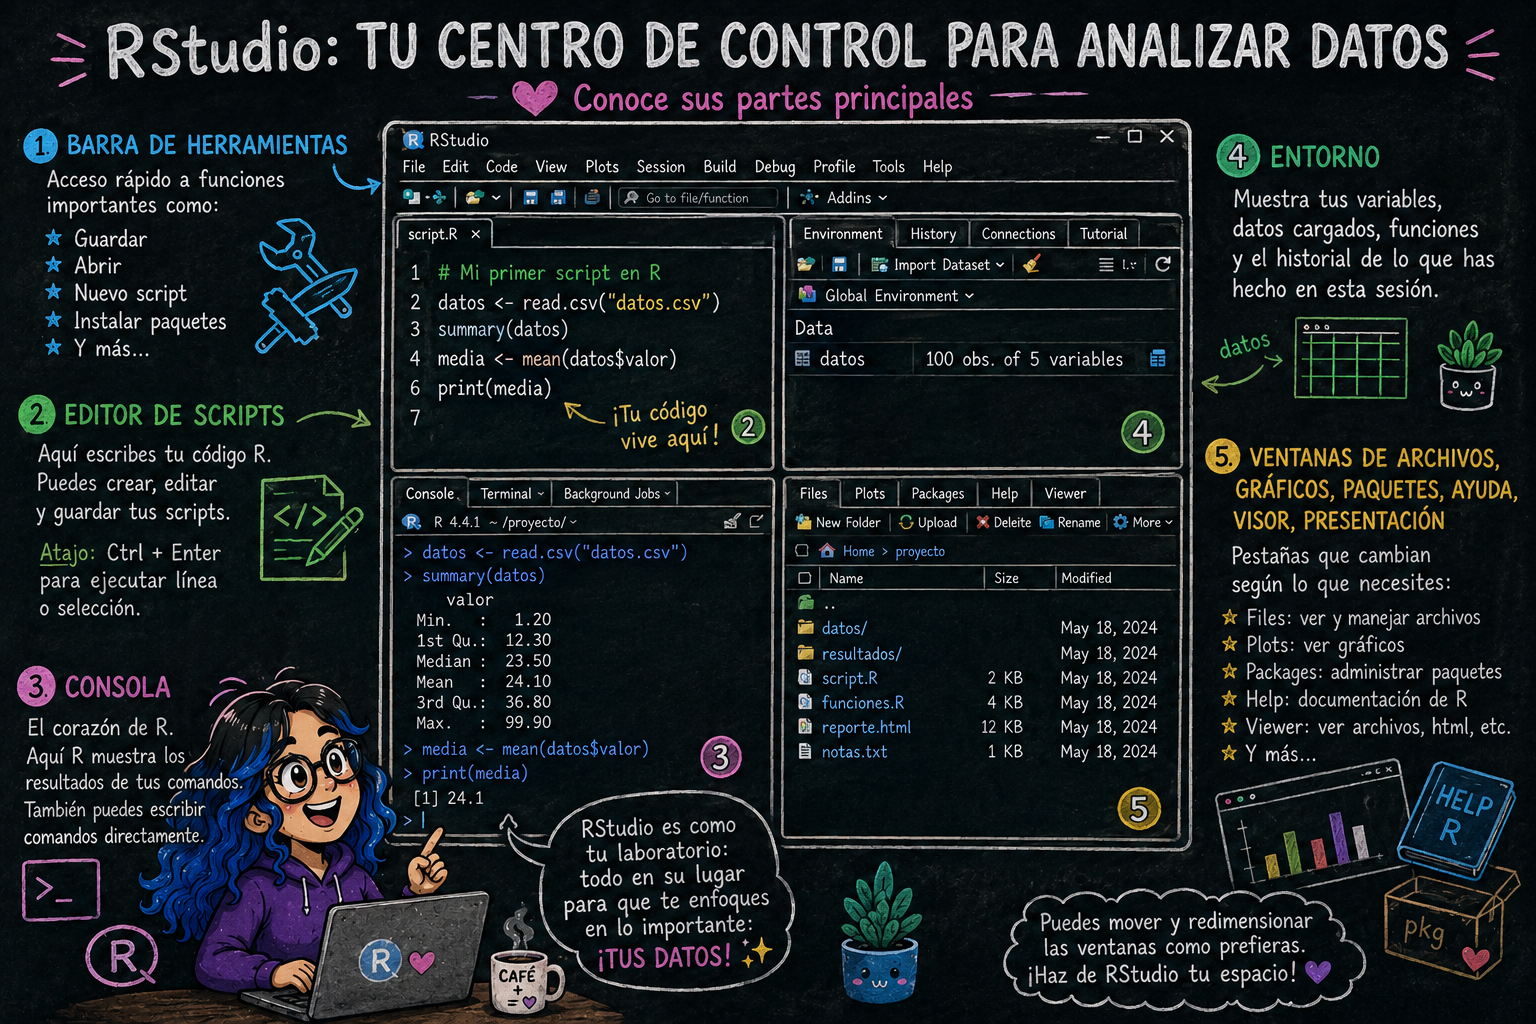
\includegraphics[keepaspectratio]{figures/rstudio_paneles.png}}

}

\caption{Imagen creada con ChatGPT.}

\end{figure}%

\section{Cambiando el aspecto de
RStudio}\label{cambiando-el-aspecto-de-rstudio}

Podemos cambiar la forma en que se ve la aplicación desde \textbf{Editar
\textgreater{} Preferencias \textgreater{} Apariencia}, escogemos el
tema que nos guste y damos click en \textbf{Aplicar} y luego \textbf{OK}

\pandocbounded{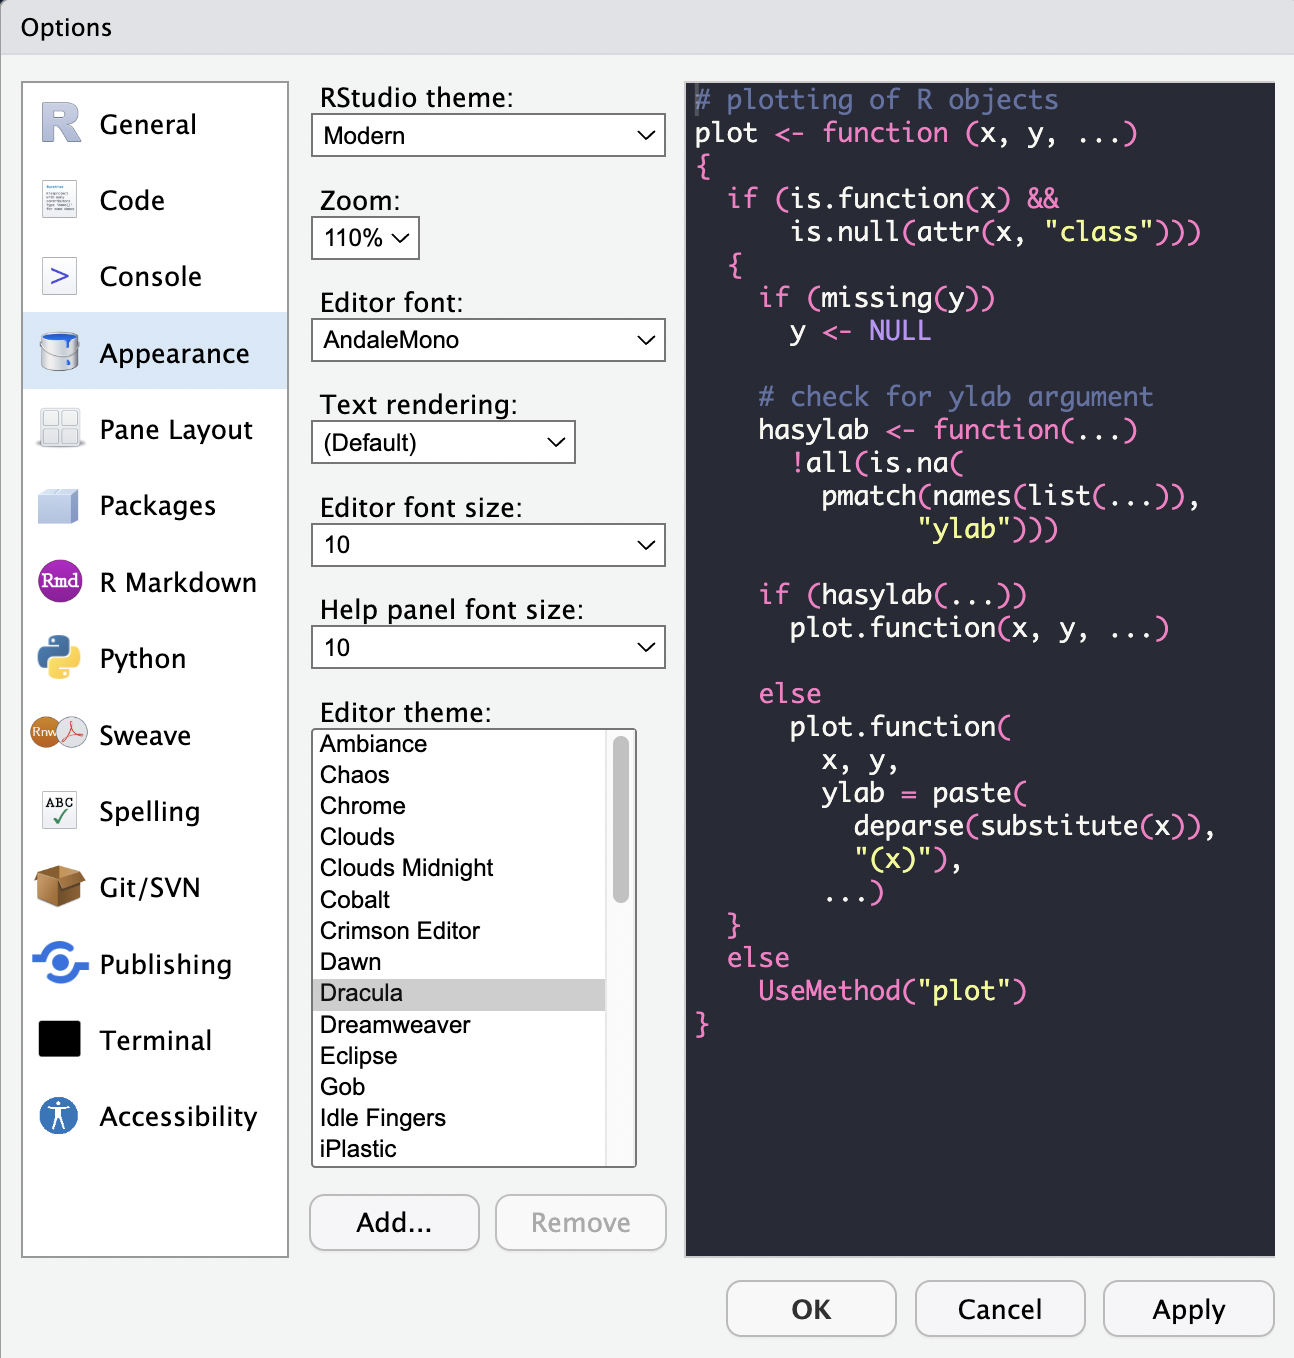
\includegraphics[keepaspectratio]{figures/apariencia-rstudio.png}}

\begin{center}
\pandocbounded{
\includegraphics[keepaspectratio]{figures/blackwindows.jpeg}}
\end{center}

\chapter{Instalación de Python y reticulate en
Rstudio}\label{instalaciuxf3n-de-python-y-reticulate-en-rstudio}

\begin{quote}
\textbf{Fecha:} 08 de septiembre, 2026
\end{quote}

\section{Windows - Python}\label{windows---python}

\begin{itemize}
\item
  Descargar desde
  \href{https://www.python.org/downloads/windows/}{python.org} o
  instalar vía Microsoft Store.
\item
  Durante la instalación, marcar la opción \textbf{``Add Python to
  PATH''}.
\item
  Alternativa recomendada: usar
  \texttt{reticulate::install\_miniconda()} desde RStudio para crear un
  entorno aislado.
\item
  Verificar instalación:
\end{itemize}

\begin{Shaded}
\begin{Highlighting}[]
\ExtensionTok{python} \AttributeTok{{-}{-}version}
\ExtensionTok{pip} \AttributeTok{{-}{-}version}
\end{Highlighting}
\end{Shaded}

\section{macOS - Python}\label{macos---python}

\begin{itemize}
\item
  \textbf{Opción Homebrew} (más sencilla y actualizada):

  En la terminal de \texttt{Bash}:

\begin{verbatim}
brew install python
python3 --version # Python 3.12.13
\end{verbatim}
\item
  \textbf{Opción instalador oficial}: descargar el \texttt{.pkg} desde
  \href{https://www.python.org/downloads/mac-osx/}{python.org}.
\item
  Importante: no usar el Python que viene con macOS en
  \texttt{/usr/bin/python3}, ya que es antiguo y reservado para el
  sistema.
\item
  Tras instalar, agregar al \textbf{PATH} si es necesario. En la
  terminal de \texttt{Bash}:

\begin{verbatim}
export PATH="/usr/local/bin:$PATH" # NO corras esto
\end{verbatim}
\end{itemize}

\section{Linux - Python}\label{linux---python}

\begin{itemize}
\item
  \textbf{Debian/Ubuntu}:

  bash

\begin{verbatim}
sudo apt update
sudo apt install python3 python3-pip
\end{verbatim}
\item
  \textbf{Fedora/RHEL}:

\begin{verbatim}
sudo dnf install python3 python3-pip
\end{verbatim}
\item
  \textbf{Recomendación avanzada}: usar pyenv para manejar múltiples
  versiones sin tocar el Python del sistema.

\begin{verbatim}
curl https://pyenv.run | bash
pyenv install 3.12.3
pyenv global 3.12.3
\end{verbatim}
\end{itemize}

\section{Integración con RStudio con
Reticulate}\label{integraciuxf3n-con-rstudio-con-reticulate}

\begin{enumerate}
\def\labelenumi{\arabic{enumi}.}
\tightlist
\item
  Instalar el paquete \texttt{reticulate} en R, coloca en la consola el
  siguiente código:
\end{enumerate}

\begin{Shaded}
\begin{Highlighting}[]
\FunctionTok{install.packages}\NormalTok{(}\StringTok{"reticulate"}\NormalTok{)}
\end{Highlighting}
\end{Shaded}

\begin{enumerate}
\def\labelenumi{\arabic{enumi}.}
\setcounter{enumi}{1}
\tightlist
\item
  En la terminal de Bash busca la ubicación de Python3
\end{enumerate}

\begin{Shaded}
\begin{Highlighting}[]
\FunctionTok{which}\NormalTok{ python3}
\end{Highlighting}
\end{Shaded}

En mi caso se encuentra en:
\texttt{/Users/ecoss/.cache/uv/archive-v0/cb\_IldkfR46NZ8HFdegcN/bin/python3}

\begin{enumerate}
\def\labelenumi{\arabic{enumi}.}
\setcounter{enumi}{2}
\tightlist
\item
  Configurar la versión de Python en RStudio: Menú: \textbf{Tools
  \textgreater{} Global Options \textgreater{} Python} → pega la
  ubicación que obtuviste.
\item
  Reinicia la Sesión de Rstudio y revisa la configuración:
\end{enumerate}

\begin{Shaded}
\begin{Highlighting}[]
\FunctionTok{library}\NormalTok{(reticulate)}
\FunctionTok{py\_config}\NormalTok{()}
\end{Highlighting}
\end{Shaded}

\begin{verbatim}
python:         /Users/ecoss/.cache/uv/archive-v0/cb_IldkfR46NZ8HFdegcN/bin/python
libpython:      /Users/ecoss/.local/share/uv/python/cpython-3.12.13-macos-aarch64-none/lib/libpython3.12.dylib
pythonhome:     /Users/ecoss/.cache/uv/archive-v0/cb_IldkfR46NZ8HFdegcN:/Users/ecoss/.cache/uv/archive-v0/cb_IldkfR46NZ8HFdegcN
virtualenv:     /Users/ecoss/.cache/uv/archive-v0/cb_IldkfR46NZ8HFdegcN/bin/activate_this.py
version:        3.12.13 (main, Apr 14 2026, 14:33:40) [Clang 22.1.3 ]
numpy:          /Users/ecoss/.cache/uv/archive-v0/cb_IldkfR46NZ8HFdegcN/lib/python3.12/site-packages/numpy
numpy_version:  2.5.1

NOTE: Python version was forced by VIRTUAL_ENV
\end{verbatim}

En la consola debe aparecerte algo así:

\begin{center}
\pandocbounded{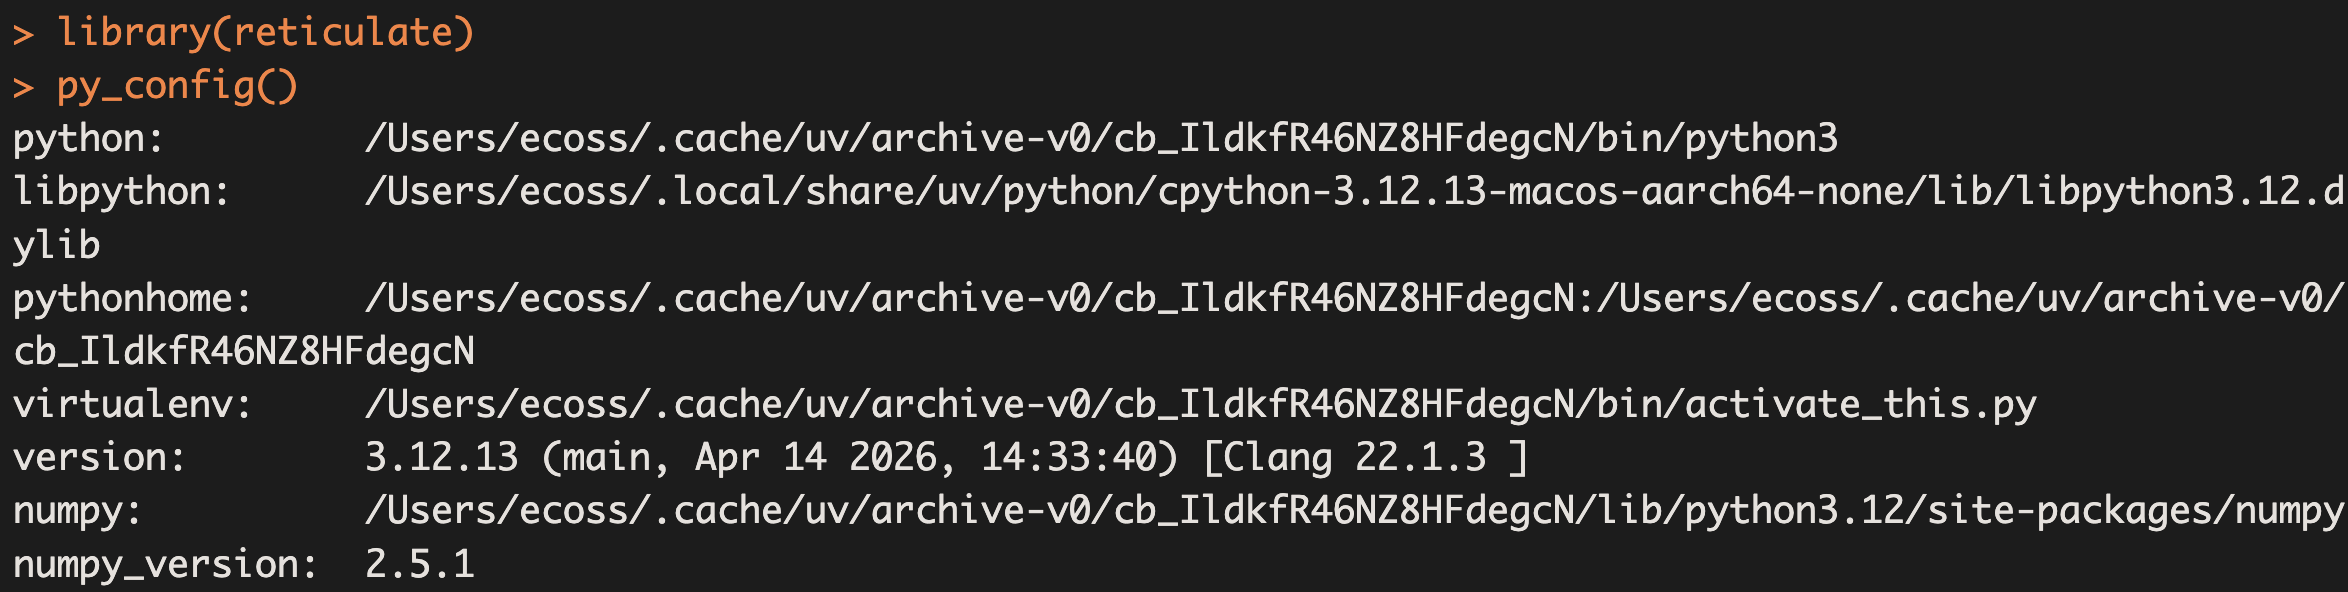
\includegraphics[keepaspectratio]{figures/rstudio_install_python.png}}
\end{center}

Visualización del uso de Python en Rstudio con Reticulate.

\begin{figure}[H]

{\centering \pandocbounded{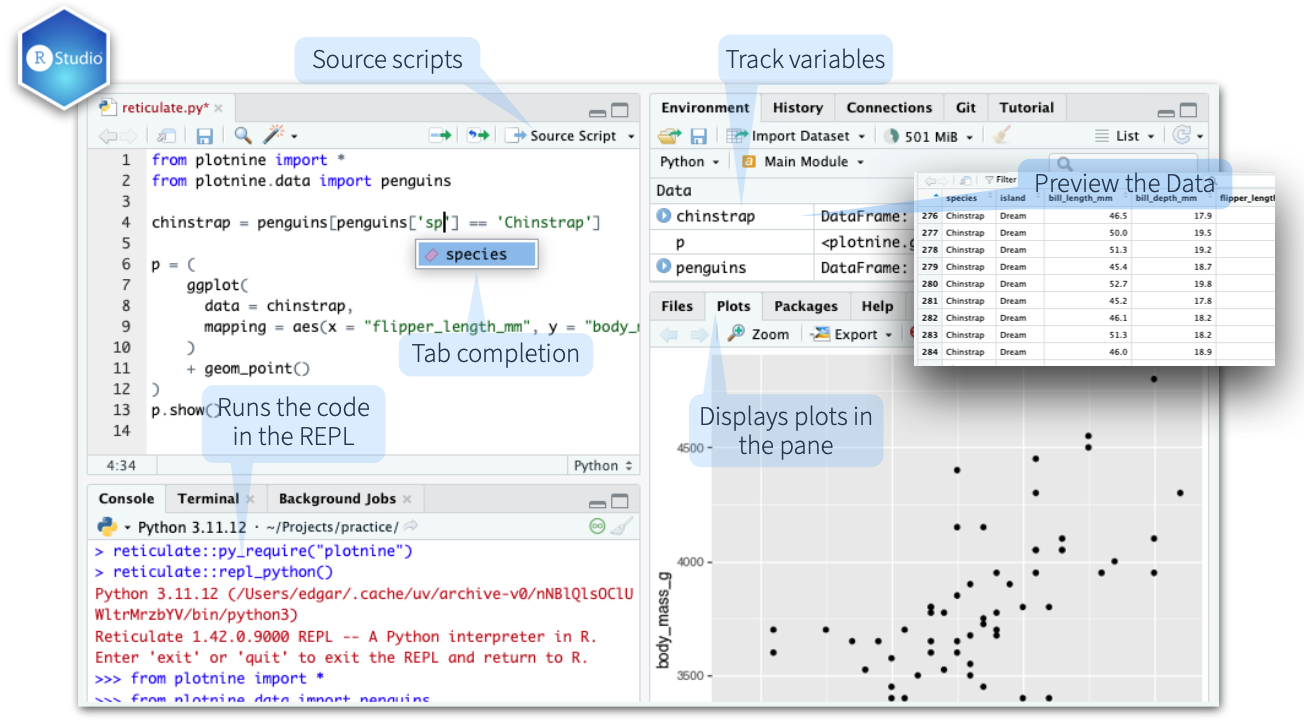
\includegraphics[keepaspectratio]{figures/rstudio_python_ambiente.png}}

}

\caption{Imagen tomada de POSIT Reticulate}

\end{figure}%

\begin{figure}[H]

{\centering \pandocbounded{
\includegraphics[keepaspectratio]{figures/python_finish.png}}

}

\caption{Imagen creada con ChatGPT.}

\end{figure}%

\section{Referencias}\label{referencias-4}

\begin{itemize}
\tightlist
\item
  \href{https://rstudio.github.io/cheatsheets/html/reticulate.html}{Guía
  de reticulate}
\item
  \href{https://rstudio.github.io/cheatsheets/translations/spanish/reticulate_es.pdf}{Usar
  Python con R con reticulate : : GUÍA RÁPIDA}
\end{itemize}

\chapter{Integración de Bash en la terminal de
Rstudio}\label{integraciuxf3n-de-bash-en-la-terminal-de-rstudio}

\begin{quote}
\textbf{Fecha:} 08 de septiembre, 2026
\end{quote}

En RStudio puedes abrir una terminal desde el menú: \textbf{Tools →
Global options → Terminal →} Elegir en \textbf{New terminals open with →
BASH}

\pandocbounded{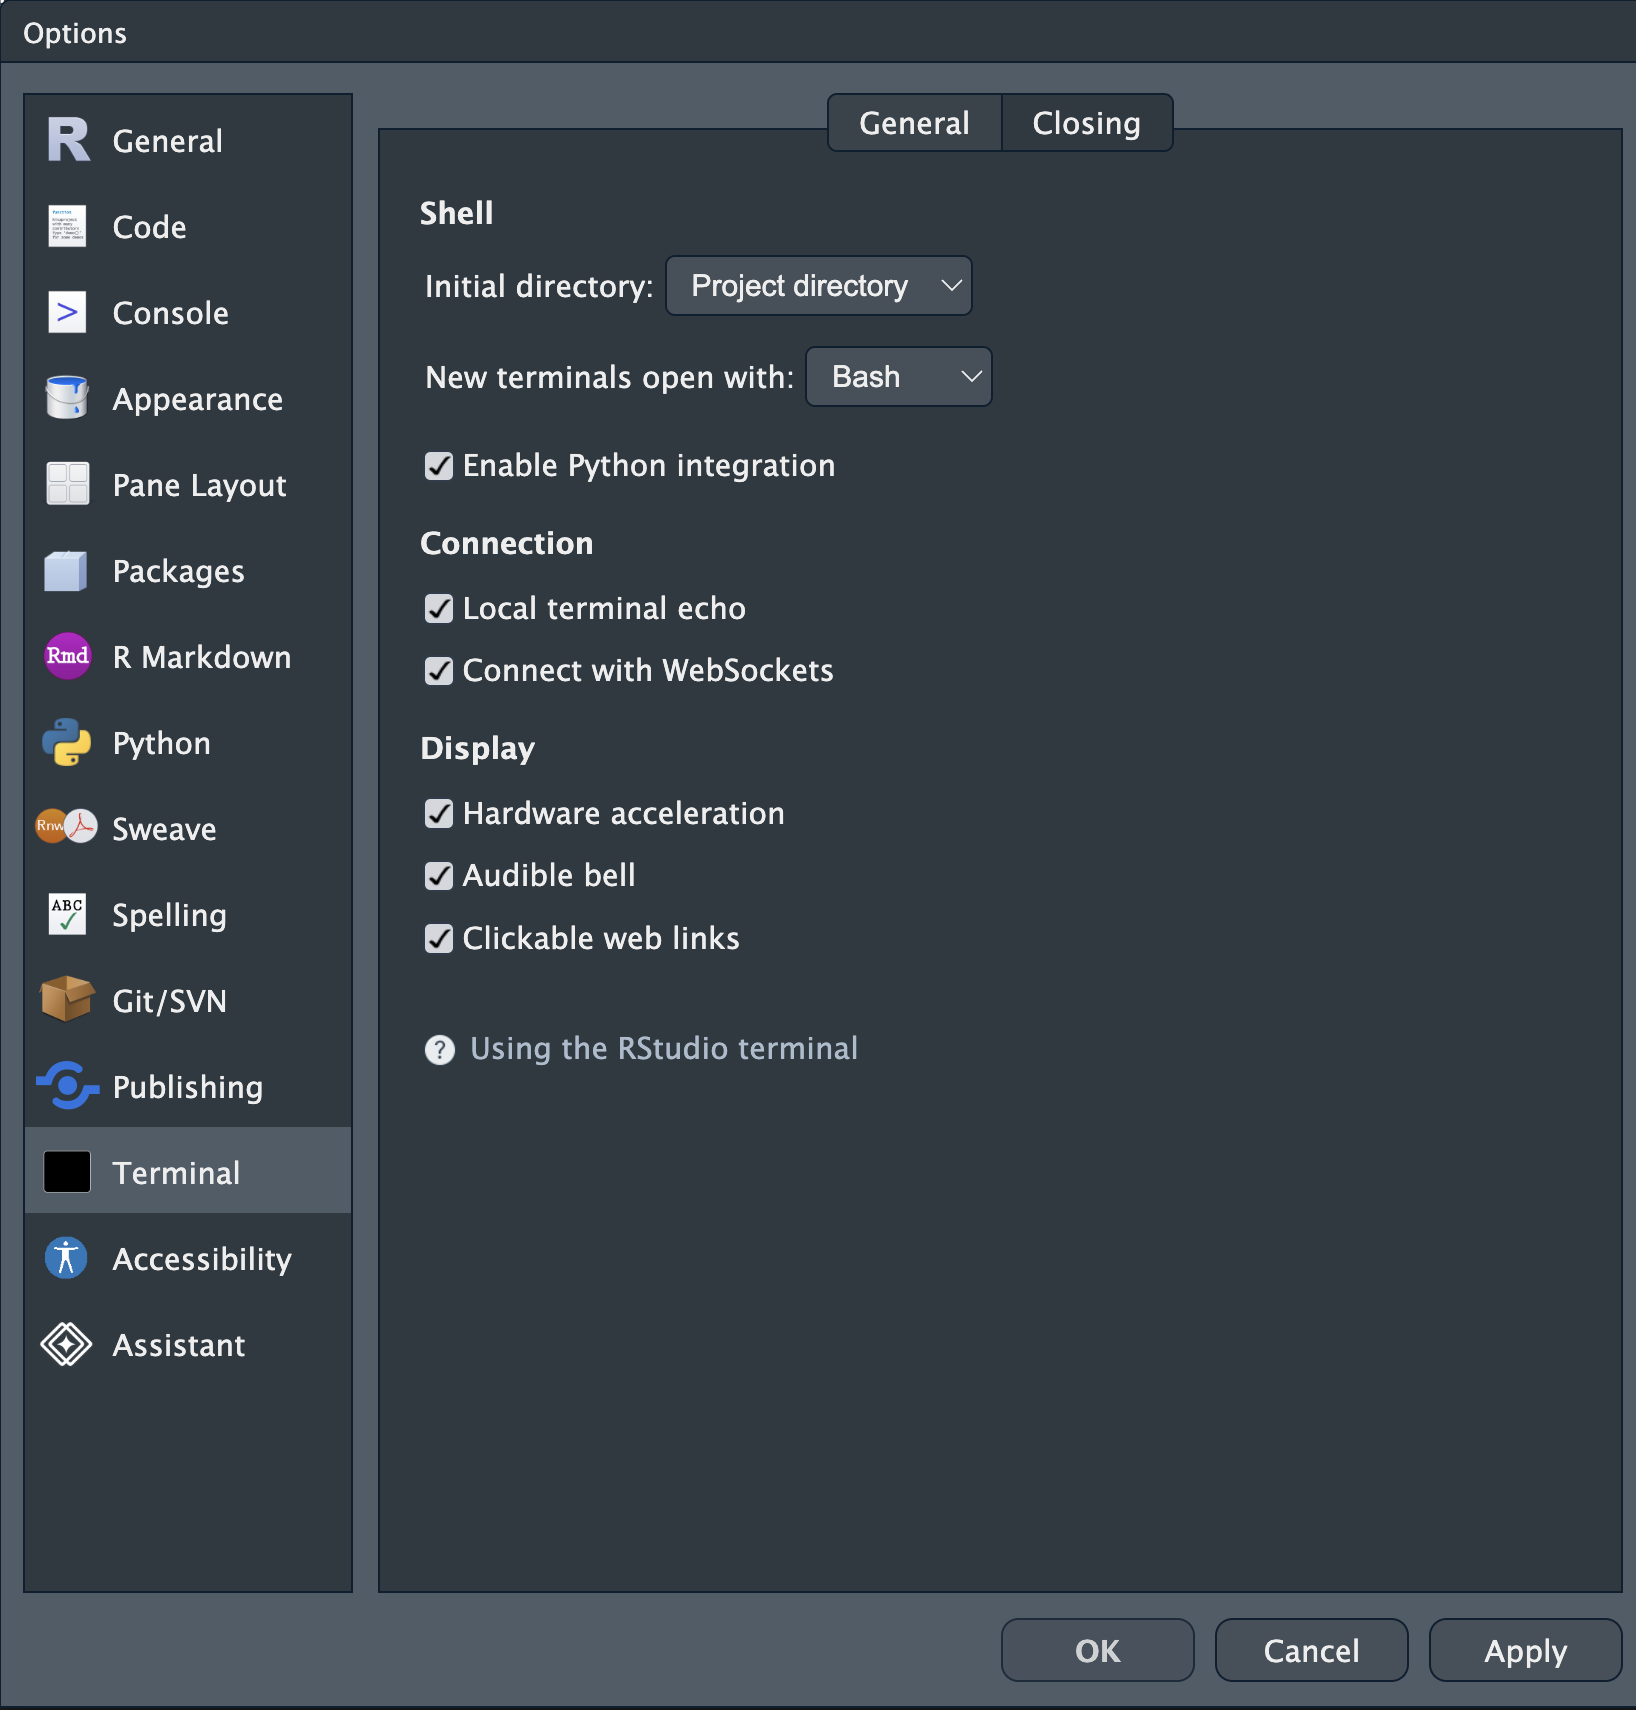
\includegraphics[keepaspectratio]{figures/rstudio_bash.png}}

\subsection{\texorpdfstring{\textbf{Windows - Terminal
Rstudio}}{Windows - Terminal Rstudio}}\label{windows---terminal-rstudio}

\begin{itemize}
\item
  Por defecto, RStudio abre \textbf{PowerShell} o \textbf{Command Prompt
  (cmd.exe)}.
\item
  Si instalaste \textbf{Git for Windows}, también se instala \textbf{Git
  Bash}.
\item
  En ese caso, RStudio detecta Git Bash y lo ofrece como opción en la
  terminal.
\item
  Puedes configurar qué shell usar en: \textbf{Tools → Global Options →
  Terminal → New terminals open with\ldots{}} Allí eliges \emph{Git
  Bash}.
\end{itemize}

👉 Con Git Bash tendrás un entorno más parecido a Linux/macOS, ideal
para enseñar comandos Bash.

\subsection{\texorpdfstring{\textbf{macOS - Terminal
Rstudio}}{macOS - Terminal Rstudio}}\label{macos---terminal-rstudio}

\begin{itemize}
\tightlist
\item
  La terminal de RStudio abre el shell por defecto del sistema.
\item
  En RStudio \textbf{no necesitas instalar nada extra}: Bash ya viene
  incluido en macOS.
\end{itemize}

\begin{figure}[H]

{\centering \pandocbounded{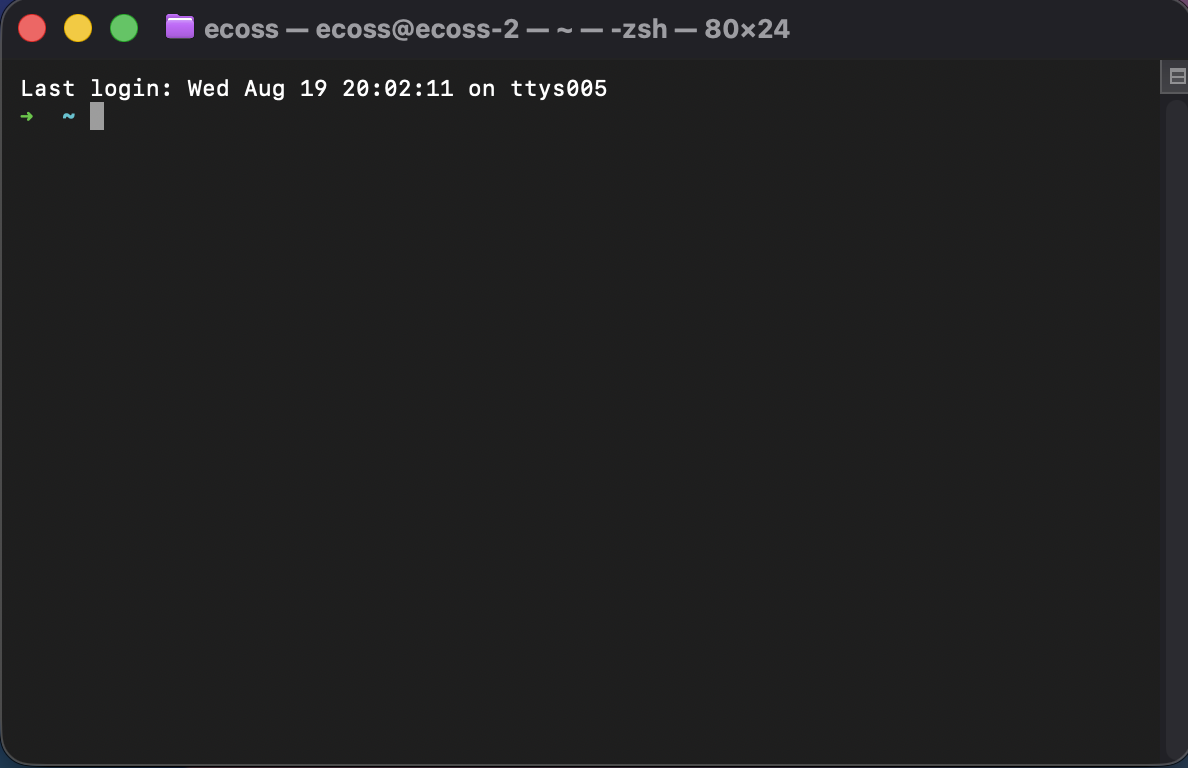
\includegraphics[keepaspectratio]{figures/entorno_bash.png}}

}

\caption{Entorno de la terminal de macOs.}

\end{figure}%

\subsection{\texorpdfstring{\textbf{Linux - Terminal
Rstudio}}{Linux - Terminal Rstudio}}\label{linux---terminal-rstudio}

\begin{itemize}
\tightlist
\item
  Igual que en macOS, la terminal abre el shell por defecto del sistema.
\item
  Normalmente es \textbf{bash}, aunque algunas distribuciones usan
  \textbf{zsh}.
\end{itemize}

\begin{figure}[H]

{\centering \pandocbounded{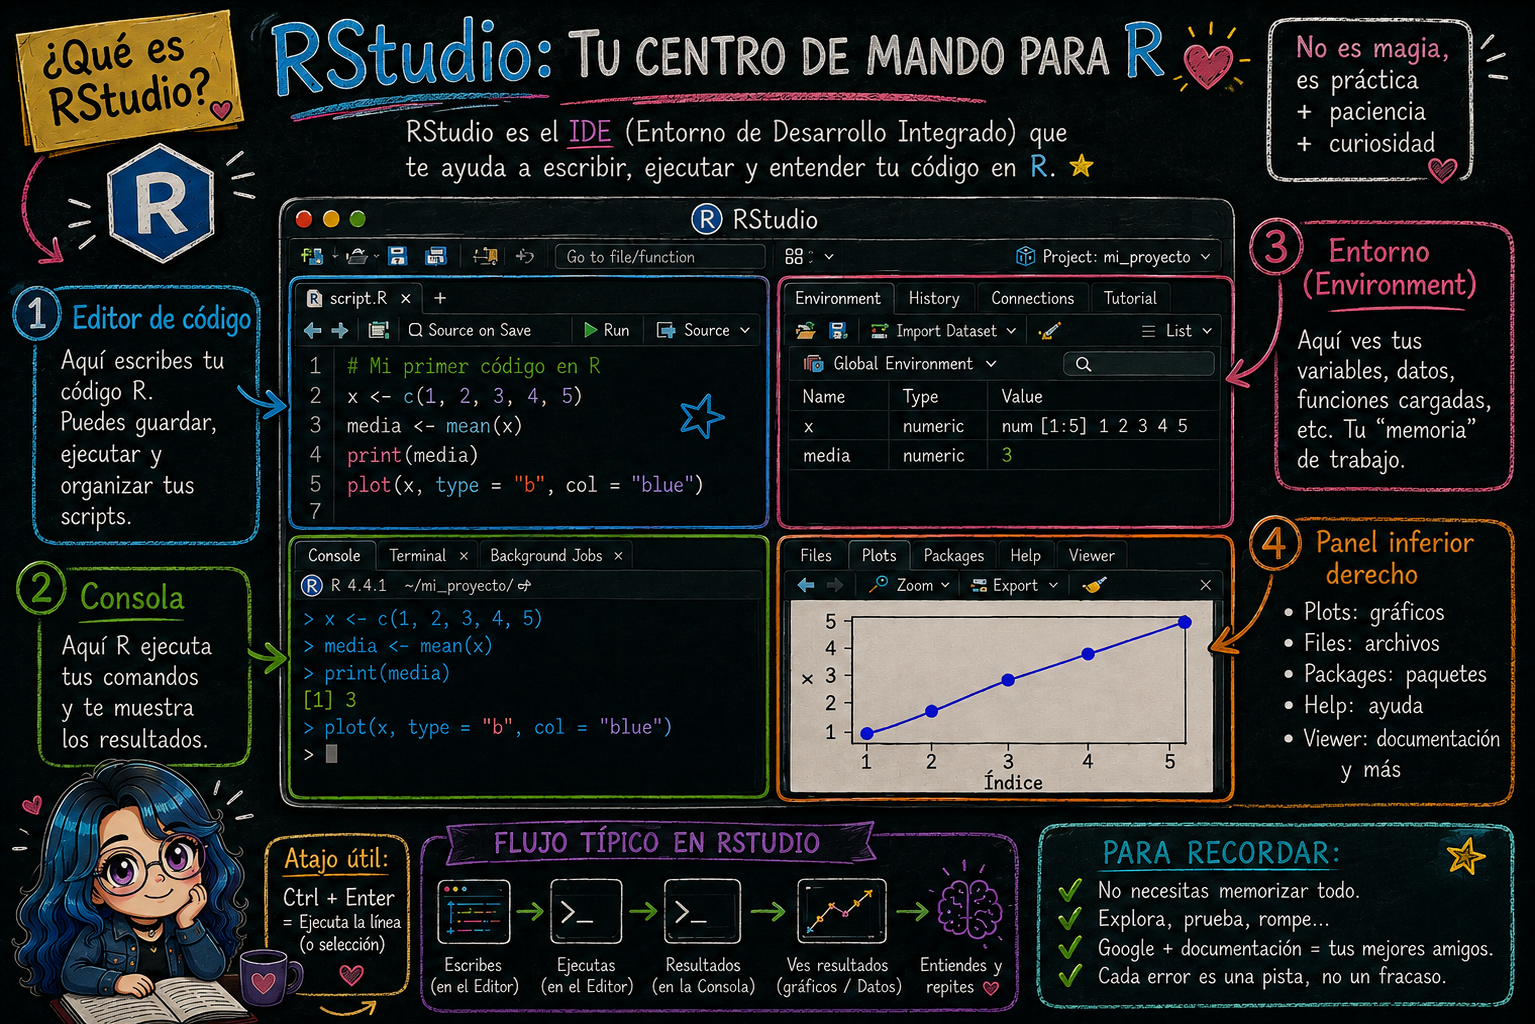
\includegraphics[keepaspectratio]{figures/Rstudio_todoenuno.png}}

}

\caption{Imagen creada con ChatGPT.}

\end{figure}%

\part{\textbf{Sección 3} - Introducción a Bash}

\chapter{Introducción a Linux/Unix}\label{introducciuxf3n-a-linuxunix}

\begin{quote}
\textbf{Fecha:} 10 de septiembre, 2026
\end{quote}

\textbf{Objetivos:}

\begin{enumerate}
\def\labelenumi{\arabic{enumi}.}
\tightlist
\item
  Comprender la historia y filosofía de Linux/Unix
\item
  Entender qué es GNU y su importancia en el software libre
\item
  Diferenciar entre Linux, GNU y GNU/Linux
\item
  Reconocer las principales versiones y distribuciones de GNU/Linux
\item
  Valorar la importancia del software libre y de código abierto
\item
  Aplicar este conocimiento en la selección de sistemas operativos
\end{enumerate}

\section{¿Qué es UNIX?}\label{quuxe9-es-unix}

\begin{itemize}
\tightlist
\item
  Sistema operativo (SO) creado por \textbf{Ken Thompson y Dennis
  Ritchie} de la empresa \emph{Bell Laboratories} de AT\&T en 1969.
\item
  Es uno de los sistemas operativos \textbf{más influyentes en la
  historia} de la computación y ha servido como base para muchos
  sistemas operativos modernos.
\end{itemize}

\subsection{\texorpdfstring{\textbf{Características principales de
Unix:}}{Características principales de Unix:}}\label{caracteruxedsticas-principales-de-unix}

\begin{itemize}
\tightlist
\item
  \textbf{Portabilidad}: Fue diseñado para funcionar en diferentes tipos
  de hardware, lo que permitió su adopción generalizada.
\item
  \textbf{Modularidad}: Sigue la filosofía ``hacer una cosa y hacerla
  bien'', donde cada programa tiene una función específica.
\item
  \textbf{Multitarea y multiusuario}: Permite que múltiples usuarios
  trabajen simultáneamente en el mismo sistema, y que múltiples procesos
  se ejecuten al mismo tiempo.
\item
  \textbf{Interfaz de línea de comandos (CLI)}: Utiliza un shell
  (intérprete de comandos) para que los usuarios interactúen con el
  sistema.
\item
  \textbf{Seguridad}: Implementa un sistema de permisos y usuarios para
  proteger los archivos y recursos del sistema.
\end{itemize}

\begin{figure}[H]

{\centering \pandocbounded{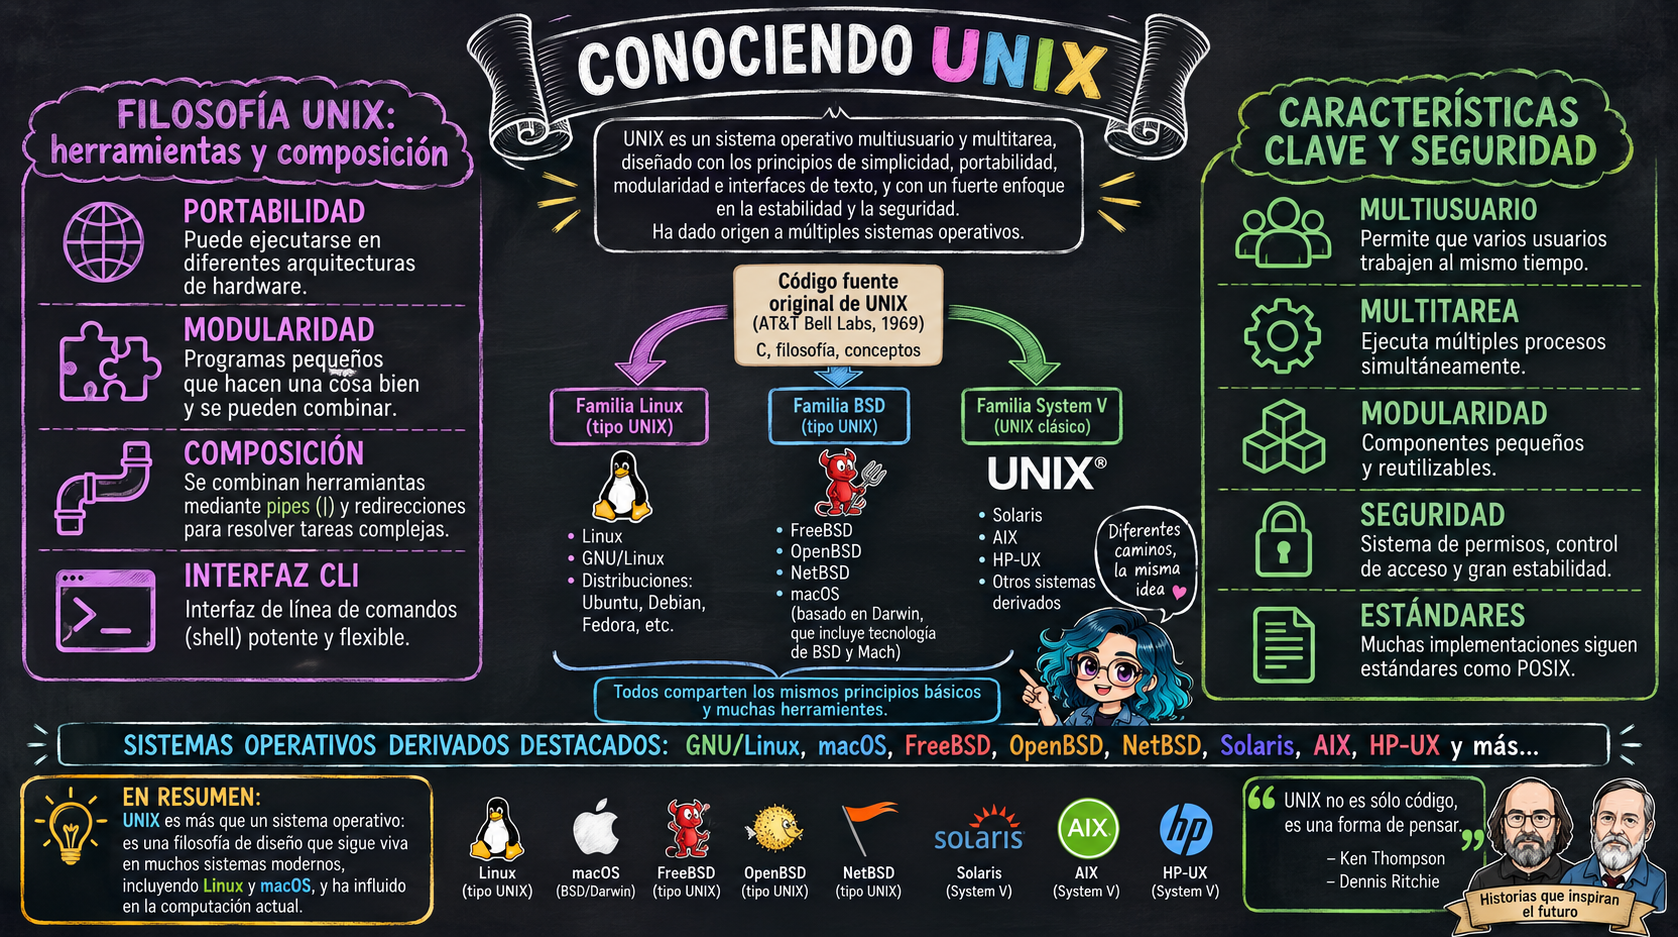
\includegraphics[keepaspectratio]{figures/Conociendo_unix.png}}

}

\caption{Imagen creada con Gemini.}

\end{figure}%

\section{GNU/Linux}\label{gnulinux}

\begin{itemize}
\tightlist
\item
  En 1983 \textbf{Richard Stallman} lideró la iniciativa
  \href{https://www.gnu.org/}{GNU} (GNU's Not Unix), SO compatible con
  UNIX de libre distribución y acceso sin restricciones al código
  fuente.
\item
  En 1991 \textbf{Linus Torvalds} creó su propio
  \href{https://linuxjourney.com/lesson/kernel-overview}{kernel}
  (Linux), que es la parte del SO que permite la comunicación con los
  componentes de Hardware. Este kernel fue distribuido de forma libre y
  gratuita.
\item
  Ambos proyectos se juntaron y se creó \textbf{GNU/Linux}
\end{itemize}

\hfill
\pandocbounded{
\includegraphics[keepaspectratio]{figures/GNU_LIN1.png}}

En resumen \ldots{}

\begin{figure}[H]

{\centering \pandocbounded{
\includegraphics[keepaspectratio]{figures/GNU:linux_flyer.png}}

}

\caption{Imagen generada con Gemini.}

\end{figure}%

\section{Filosofía GNU/Linux}\label{filosofuxeda-gnulinux}

\begin{itemize}
\tightlist
\item
  Los usuarios son libres de \textbf{ejecutar, copiar, distribuir,
  estudiar, cambiar y mejorar} el software.
\item
  El \href{https://www.gnu.org/philosophy/free-sw.html}{software libre}
  se refiere a las libertades mencionadas, no al precio.
\item
  \href{https://opensource.org/}{``open source''} vs
  \href{https://www.gnu.org/philosophy/free-sw.html}{``free software''}.
\end{itemize}

\begin{figure}[H]

{\centering \pandocbounded{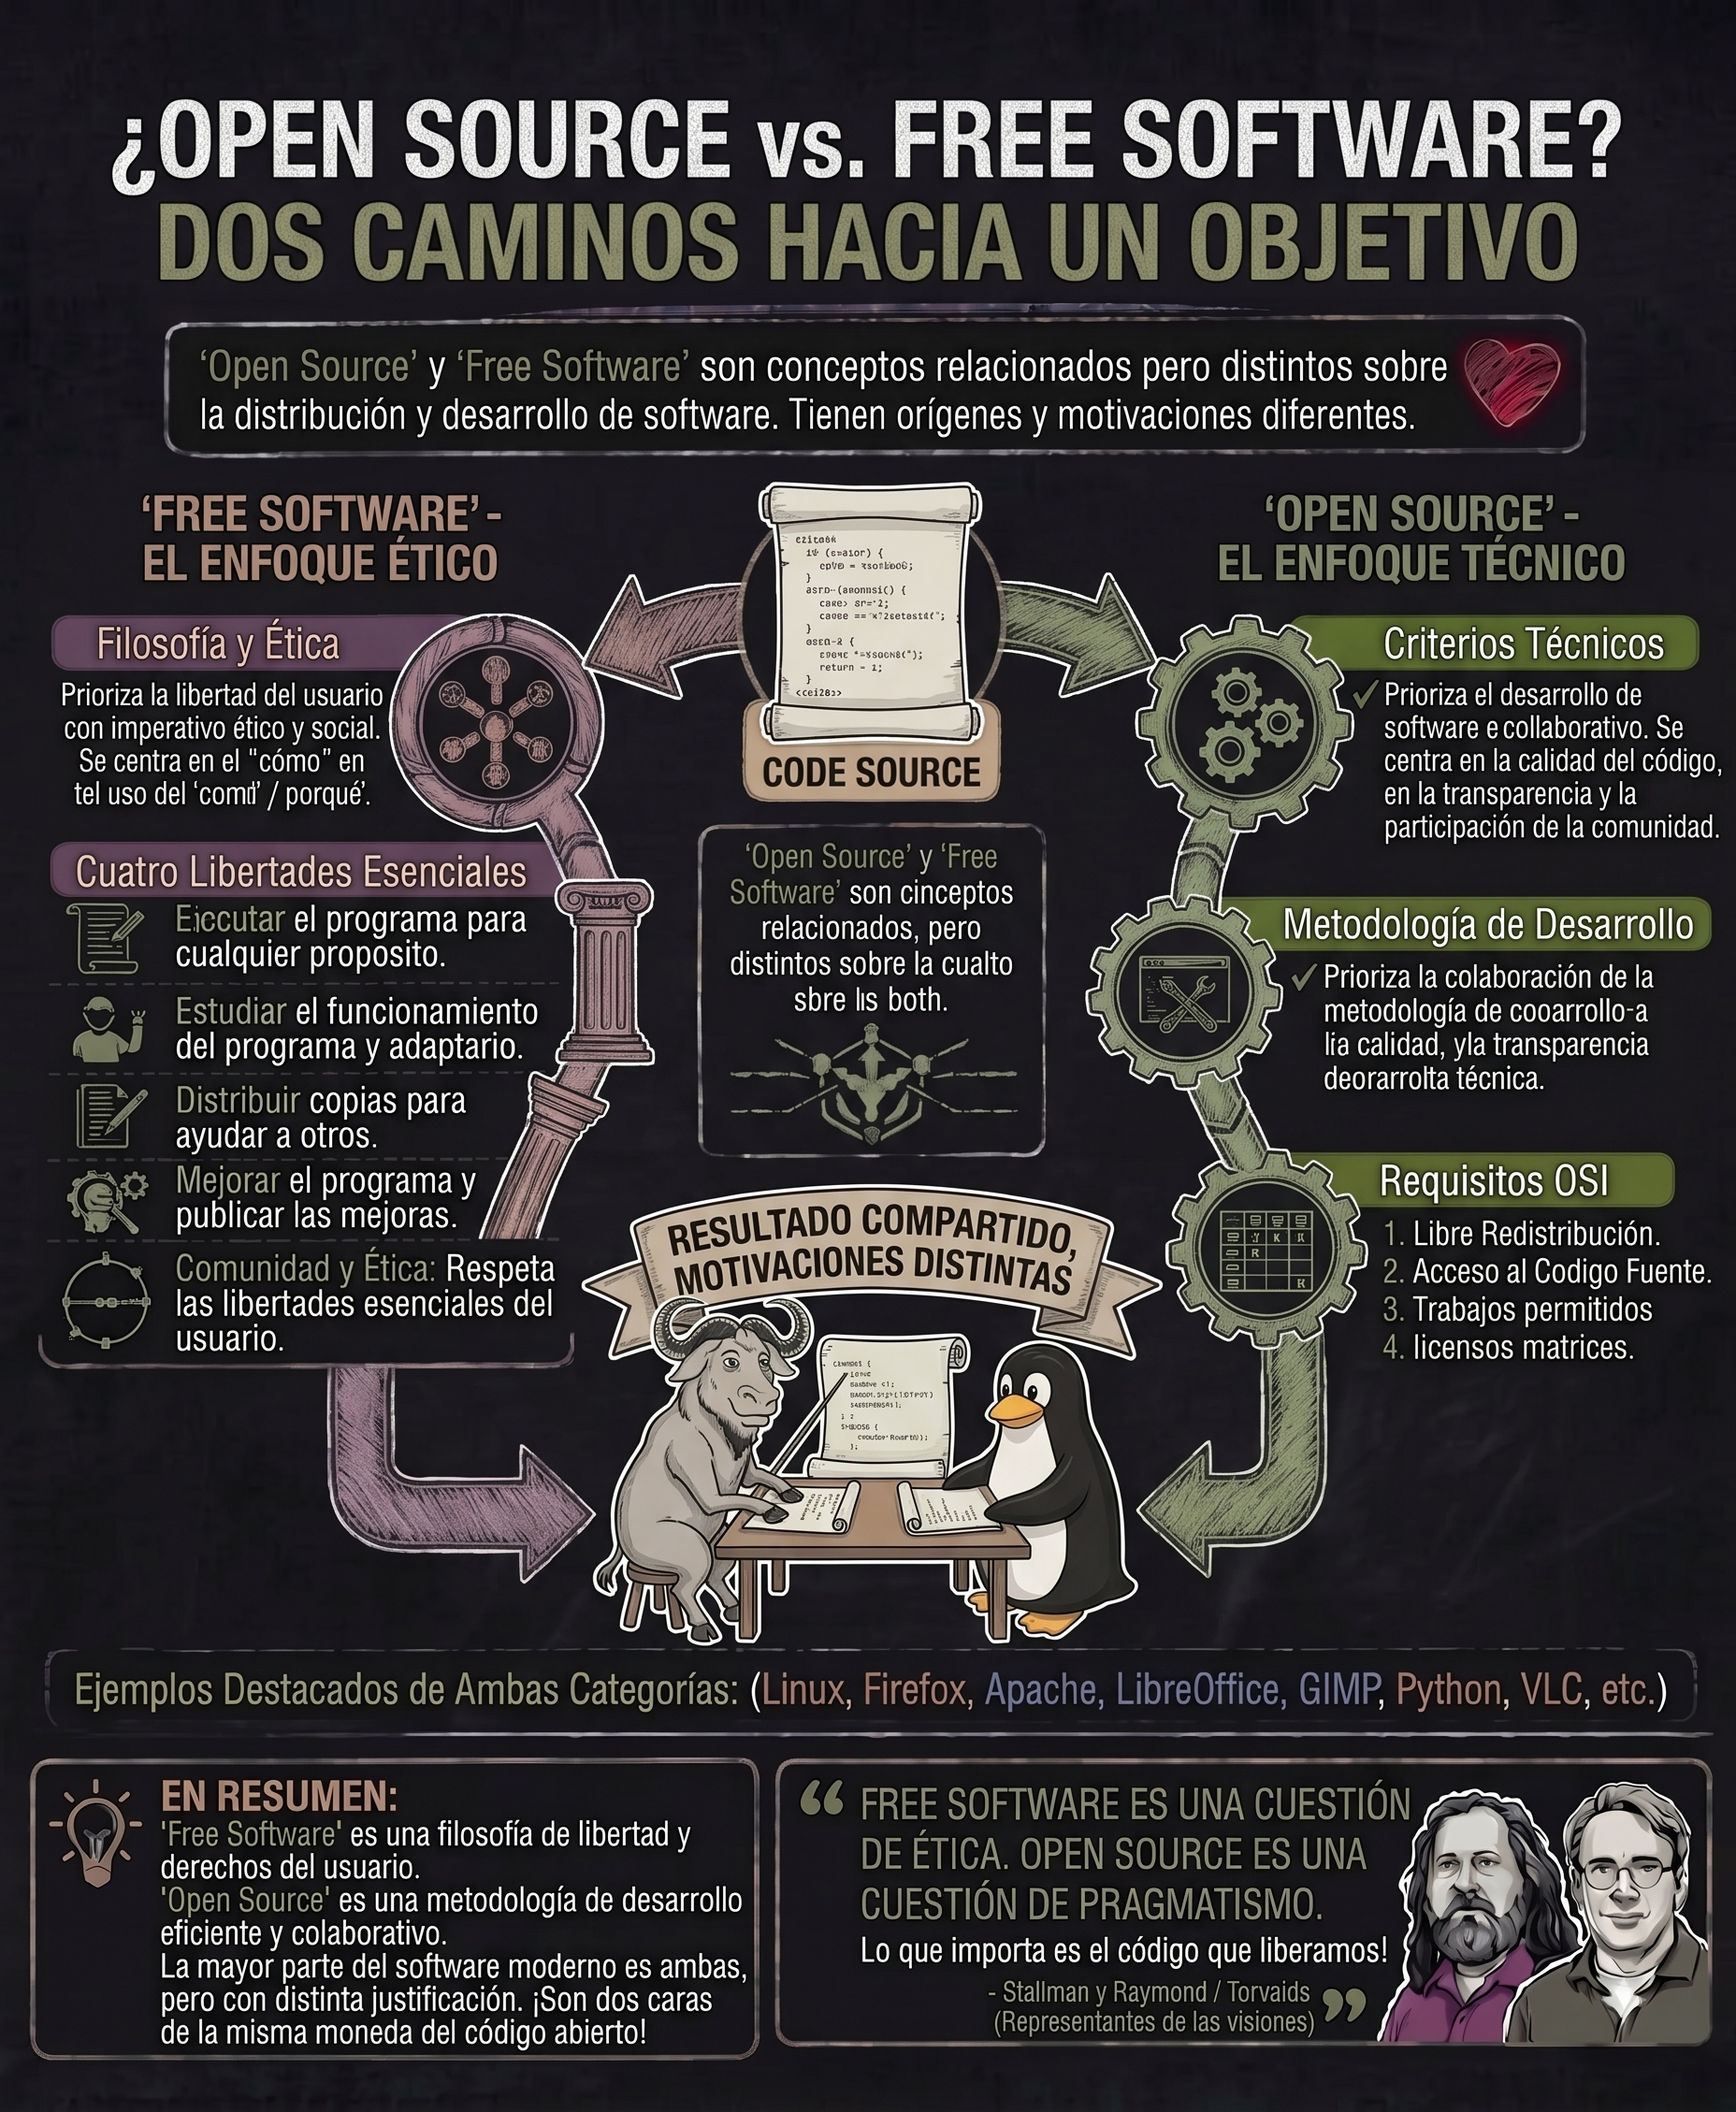
\includegraphics[keepaspectratio]{figures/Opensorce.png}}

}

\caption{Imagen creada con Gemini.}

\end{figure}%

\section{Ubuntu}\label{ubuntu}

\begin{itemize}
\tightlist
\item
  Una de las distribuciones de GNU/Linux más populares.
\item
  Está basada en \href{https://www.debian.org/}{Debian} y fue
  desarrollada por la empresa
  \href{https://canonical.com/}{\emph{Canonical}}
\item
  Facilidad de uso e instalación.
\item
  Interfaz de usuario amigable.
\end{itemize}

\begin{center}

\includegraphics[width=2.13542in,height=\textheight,keepaspectratio]{figures/ubuntu.png}
\end{center}

\section{Shell / Bash / Bash Shell}\label{shell-bash-bash-shell}

\begin{itemize}
\tightlist
\item
  La \href{https://en.wikipedia.org/wiki/Unix_shell}{\emph{shell}} es el
  programa que provee una \textbf{interfaz de línea de comandos (CLI)},
  que permite la comunicación entre el usuario y el SO.
\item
  La mayoría de distribuciones de Linux tienen por defecto
  \href{https://www.gnu.org/software/bash/}{\emph{bash}} (``Bourne Again
  SHell'') como \emph{shell}. Hay
  \href{https://www.educba.com/types-of-shells-in-linux/}{otros tipos de
  shell} como \texttt{sh,\ csh,\ tcsh,\ ksh,\ zsh}, entre otras.
\end{itemize}

\begin{center}

\includegraphics[width=3.78125in,height=\textheight,keepaspectratio]{figures/bash.png}
\end{center}

Bash es un intérprete de comandos que te da el poder de hacer tareas
simples rápidamente.

En resumen \ldots{}

\begin{figure}[H]

{\centering \pandocbounded{
\includegraphics[keepaspectratio]{figures/bash_overview.png}}

}

\caption{Imagen creada con ChatGPT.}

\end{figure}%

\section{Material suplementario}\label{material-suplementario}

Si quieren aprender temas más sobre UNIX, GNU/Linux, bash, emulador de
terminal y otros tema, pueden explorar los siguientes recursos, que son
de acceso libre:

\begin{itemize}
\tightlist
\item
  Kross, S. (2017). \emph{The unix workbench}. Leanpub.
  \url{https://leanpub.com/unix}
\item
  Ross, A. (2019). \emph{The Ultimate Linux Newbie Guide}.
  \url{https://linuxnewbieguide.org/}
\item
  Shotts, W. (2019). \emph{The Linux command line: a complete
  introduction}. No Starch Press.
  \url{http://www.linuxcommand.org/tlcl.php/index.php}
\item
  Linux Journey. (2020). Linux Journey. \url{https://linuxjourney.com/}
\item
  GNU. (2020). GNU. \url{https://www.gnu.org/}
\item
  \href{https://rsg-ecuador.github.io/unix.bioinfo.rsgecuador/content/Curso_basico/01_Unix_GNU-Linux/1_Conceptos_Unix_GNU_Linux.html}{GNU/Linux
  para bioinformatica}
\end{itemize}

\chapter{Mis primeros pasos en Bash}\label{mis-primeros-pasos-en-bash}

\begin{quote}
\textbf{Fecha:} 10 de septiembre, 2026
\end{quote}

\section{Entorno de Bash}\label{entorno-de-bash}

\pandocbounded{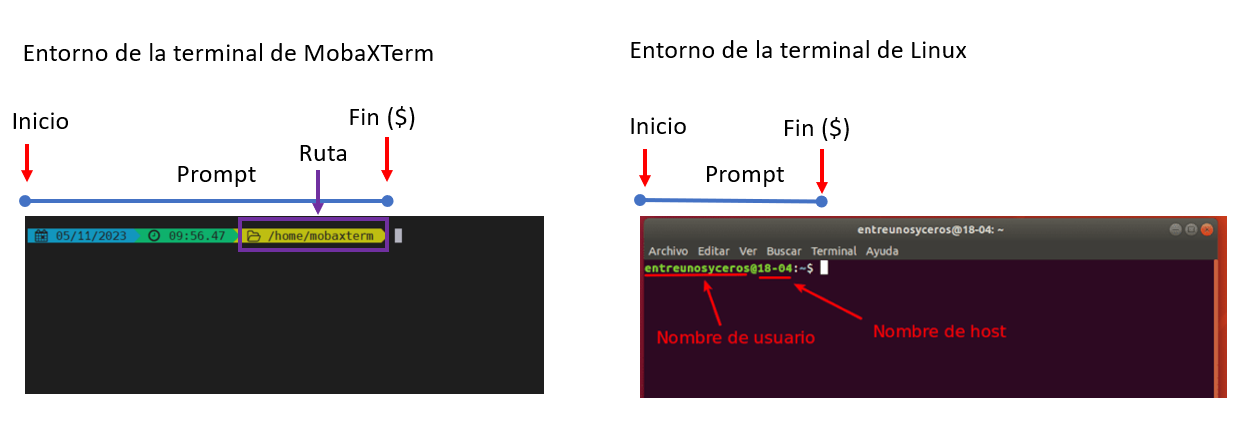
\includegraphics[keepaspectratio]{figures/entornoBash.png}}

El signo \texttt{\$} es un \textbf{prompt}, que nos muestra que la
terminal está esperando una entrada; tu terminal puede usar un carácter
diferente como prompt y puede agregar información antes de él. Al
teclear comandos, ya sea a partir de estas lecciones o de otras fuentes,
no escribas el prompt (\emph{\$}), sólo los comandos que le siguen.

\section{Entorno de zsh en macOs}\label{entorno-de-zsh-en-macos}

\begin{figure}[H]

{\centering \pandocbounded{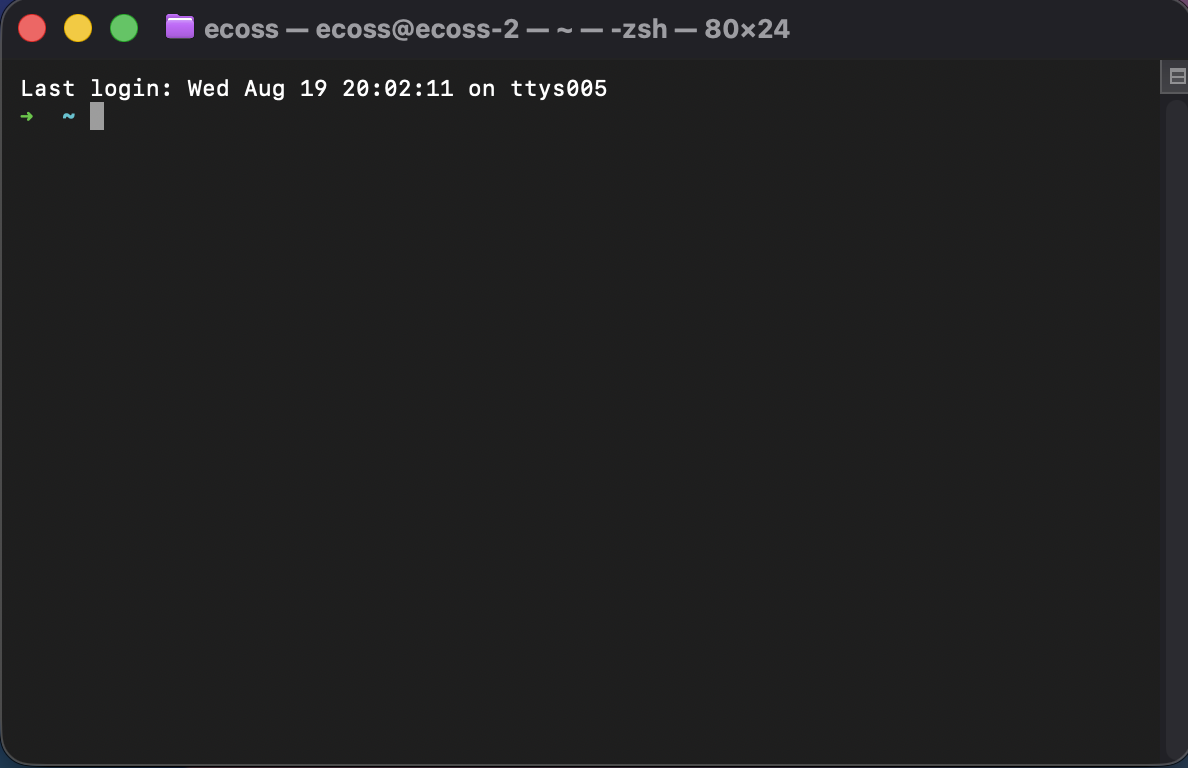
\includegraphics[keepaspectratio]{figures/entorno_bash.png}}

}

\caption{Captura de mi entorno de Bash en mi mac.}

\end{figure}%

\begin{tcolorbox}[enhanced jigsaw, arc=.35mm, bottomrule=.15mm, bottomtitle=1mm, breakable, colback=white, colbacktitle=quarto-callout-note-color!10!white, colframe=quarto-callout-note-color-frame, coltitle=black, left=2mm, leftrule=.75mm, opacityback=0, opacitybacktitle=0.6, rightrule=.15mm, title=\textcolor{quarto-callout-note-color}{\faInfo}\hspace{0.5em}{Decoración de terminal}, titlerule=0mm, toprule=.15mm, toptitle=1mm]

Puedes decorar tu terminal con \href{https://ohmyz.sh/}{oh my zsh} si
tienes macOS.

\end{tcolorbox}

\section{Preparación del directorio de
trabajo}\label{preparaciuxf3n-del-directorio-de-trabajo}

\begin{itemize}
\item
  Ruta / Camino absoluto

\begin{Shaded}
\begin{Highlighting}[]
\BuiltInTok{cd}\NormalTok{ /home/usuario/data/}
\end{Highlighting}
\end{Shaded}
\item
  Ruta / Camino relativo

\begin{Shaded}
\begin{Highlighting}[]
\BuiltInTok{cd}\NormalTok{ ../ }\CommentTok{\# Ir a la carpeta anterior}
\end{Highlighting}
\end{Shaded}
\end{itemize}

\begin{tcolorbox}[enhanced jigsaw, arc=.35mm, bottomrule=.15mm, bottomtitle=1mm, breakable, colback=white, colbacktitle=quarto-callout-note-color!10!white, colframe=quarto-callout-note-color-frame, coltitle=black, left=2mm, leftrule=.75mm, opacityback=0, opacitybacktitle=0.6, rightrule=.15mm, title=\textcolor{quarto-callout-note-color}{\faInfo}\hspace{0.5em}{Nota}, titlerule=0mm, toprule=.15mm, toptitle=1mm]

\textbf{NOTA 1:} Si das \texttt{cd} y no indicas una ruta absoluta, te
llevara al Directorio Raiz (\textasciitilde).

\textbf{NOTA 2:} Puedes usar la tecla TAB para completar el nombre de la
carpeta. En caso de que tengas más de dos carpetas que inicien igual,
tendrás que terminar de completar el nombre.

\end{tcolorbox}

\section{Conocer mi dirección /
ubicación}\label{conocer-mi-direcciuxf3n-ubicaciuxf3n}

Averiguemos dónde estamos, ejecutando el comando~\texttt{pwd}~(que
significa ``imprime directorio de trabajo'' - ``print working
directory''). En cualquier momento, nuestro~\textbf{directorio
actual}~es nuestro directorio predeterminado, es decir, el directorio
que la computadora supone queremos ejecutar comandos a menos que
especifiquemos explícitamente otra cosa. En este caso la respuesta de la
computadora es~\texttt{/Users/nelle}, el cual es el directorio de inicio
de Nelle, también conocido como su directorio~\textbf{home}:

\begin{Shaded}
\begin{Highlighting}[]
\BuiltInTok{pwd} \CommentTok{\# /c/Users/ecoss}
\end{Highlighting}
\end{Shaded}

En la computadora de Evelia, el sistema de archivos se ve así:

\href{https://swcarpentry.github.io/shell-novice-es/02-filedir.html}{\begin{center}
\pandocbounded{\includesvg[keepaspectratio]{index_files/mediabag/filesystem.svg}}
\end{center}
}

En la parte superior está el \textbf{directorio raíz} o \textbf{root}
que contiene todo lo demás. Nos referimos a este directorio usando un
caracter de barra \texttt{/} por si solo; esta es la barra al inicio de
\texttt{/Users/ecoss}.

Dentro de ese directorio hay otros directorios: \texttt{bin} (que es
donde se almacenan algunos programas preinstalados), \texttt{data} (para
archivos de datos diversos), \texttt{Users} (donde se encuentran los
directorios personales de los usuarios), \texttt{tmp} (para archivos
temporales que no necesitan ser almacenados a largo plazo), etcétera.

\begin{tcolorbox}[enhanced jigsaw, arc=.35mm, bottomrule=.15mm, bottomtitle=1mm, breakable, colback=white, colbacktitle=quarto-callout-note-color!10!white, colframe=quarto-callout-note-color-frame, coltitle=black, left=2mm, leftrule=.75mm, opacityback=0, opacitybacktitle=0.6, rightrule=.15mm, title=\textcolor{quarto-callout-note-color}{\faInfo}\hspace{0.5em}{Ejercicio 1}, titlerule=0mm, toprule=.15mm, toptitle=1mm]

A partir de \texttt{/Users/ecoss/data/}, ¿Cuál de los siguientes
comandos podría Evelia usar para navegar a su directorio de inicio, que
es \texttt{/Users/ecoss}?

\begin{enumerate}
\def\labelenumi{\arabic{enumi}.}
\item
  \texttt{cd\ .}
\item
  \texttt{cd\ /}
\item
  \texttt{cd\ /home/ecoss}
\item
  \texttt{cd\ ../..}
\item
  \texttt{cd\ \textasciitilde{}}
\item
  \texttt{cd\ home}
\item
  \texttt{cd\ \textasciitilde{}/data/..}
\item
  \texttt{cd}
\item
  \texttt{cd\ ..}

  \begin{quote}
  \textbf{Solución}

  \begin{enumerate}
  \def\labelenumii{\arabic{enumii}.}
  \item
    No: \texttt{.} significa el directorio actual.
  \item
    No: \texttt{/} significa el directorio raíz.
  \item
    No: El directorio \textbf{home} de Evelia es \texttt{/Users/ecoss}.
  \item
    No: sube dos niveles, es decir termina en \texttt{/Users}.
  \item
    Sí: \texttt{\textasciitilde{}} significa el directorio \textbf{home}
    del usuario, en este caso \texttt{/Users/amanda}.
  \item
    No: esto navegaría a un directorio \texttt{home} en el directorio
    actual, si existe.
  \item
    Sí: innecesariamente complicado, pero correcto.
  \item
    Sí: un atajo para volver al directorio \textbf{home} del usuario.
  \item
    Sí: sube un nivel.
  \end{enumerate}
  \end{quote}
\end{enumerate}

\end{tcolorbox}

Ejemplo de rutas:

\begin{figure}[H]

{\centering \pandocbounded{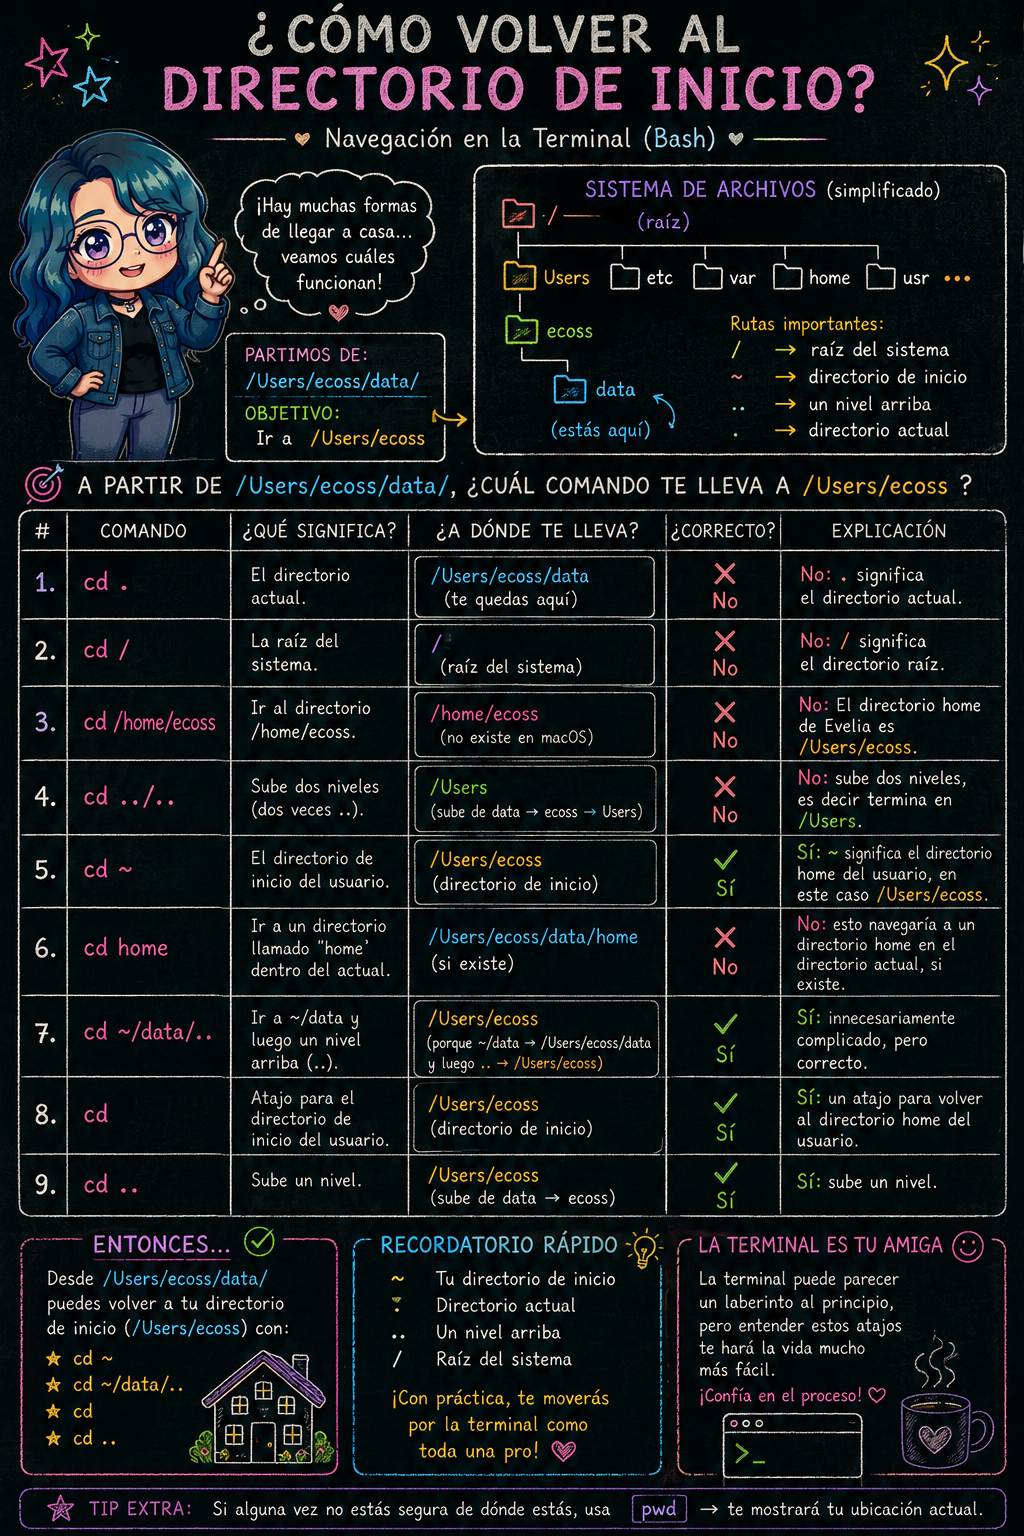
\includegraphics[keepaspectratio]{figures/bash_rutas.png}}

}

\caption{Imagen creada con Gemini.}

\end{figure}%

\section{Comandos básicos}\label{comandos-buxe1sicos}

{\def\LTcaptype{none} % do not increment counter
\begin{longtable}[]{@{}
  >{\raggedright\arraybackslash}p{(\linewidth - 4\tabcolsep) * \real{0.3333}}
  >{\raggedright\arraybackslash}p{(\linewidth - 4\tabcolsep) * \real{0.3333}}
  >{\raggedright\arraybackslash}p{(\linewidth - 4\tabcolsep) * \real{0.3333}}@{}}
\toprule\noalign{}
\begin{minipage}[b]{\linewidth}\raggedright
Comandos
\end{minipage} & \begin{minipage}[b]{\linewidth}\raggedright
Información
\end{minipage} & \begin{minipage}[b]{\linewidth}\raggedright
Argumentos
\end{minipage} \\
\midrule\noalign{}
\endhead
\bottomrule\noalign{}
\endlastfoot
\texttt{ssh} & Conexión a servidores & ssh usuario@servidor.mx \\
\texttt{ls} & Observar el contenido de los archivos en una carpeta & ls
directorio/ \\
\texttt{cd} & Moverse de directorios & cd /home/usuario/data/ \\
\texttt{mkdir} & Crear un nuevo directorio & mkdir data \\
\texttt{rmdir} & Eliminar el directorio & rmkdir -rf data \\
\texttt{nano}~/~\texttt{vim} & Editores de texto plano & nano
Archivo.txt / vim Archivo.txt \\
\texttt{cp} & Copiar archivos & cp Archivo1.txt /home/usuario/data/ \\
\texttt{mv} & Mover un archivo o carpeta & \\
\texttt{echo} & Para llamar y/o declarar variables & echo ``Hello
world'' \\
\texttt{chmod} & Cambiar permisos del usuario & chmod 777 data/ \\
\texttt{rsync} & Descargar o subir archivos & \\
\texttt{scp} & Descargar o subir archivos & \\
\texttt{cat} & Visualizar contenido de un archivo. Escribe el contenido
del archivo de manera secuencial a la salida estándar, a la ventana de
Terminal. & \\
\texttt{less} & Leer contenido de un archivo sin interrumpir la pantalla
de Terminal. Similar a~\texttt{Vim}~pero sin opción para
escribir.~\textbf{Se sale del modo visualización con}~q. & \\
\texttt{find} & Busca archivos en un directorio específico. & \\
\texttt{head} & Visualizar primeras líneas de un archivo. & \\
\texttt{tail} & Visualizar últimas líneas de un archivo. & \\
\texttt{which} & Indica el directorio donde se encuentra un particular
comando o programa que se haya podido encontrar usando los directorios
guardados en la variable de estado~\texttt{PATH}. & which bash \\
\end{longtable}
}

\begin{tcolorbox}[enhanced jigsaw, arc=.35mm, bottomrule=.15mm, bottomtitle=1mm, breakable, colback=white, colbacktitle=quarto-callout-note-color!10!white, colframe=quarto-callout-note-color-frame, coltitle=black, left=2mm, leftrule=.75mm, opacityback=0, opacitybacktitle=0.6, rightrule=.15mm, title=\textcolor{quarto-callout-note-color}{\faInfo}\hspace{0.5em}{Ayuda de funciones}, titlerule=0mm, toprule=.15mm, toptitle=1mm]

Puedes consultar mas información usando \texttt{man\ ls}

\end{tcolorbox}

\section{Consultar información sobre archivos y
directorios}\label{consultar-informaciuxf3n-sobre-archivos-y-directorios}

\subsection{\texorpdfstring{\textbf{Información
contenida}}{Información contenida}}\label{informaciuxf3n-contenida}

Cada columna en la salida anterior tiene un significado:

\href{https://eveliacoss.github.io/RNAseq_classFEB2024/Presentaciones/Dia1_AspectosGenerales.html\#74}{\pandocbounded{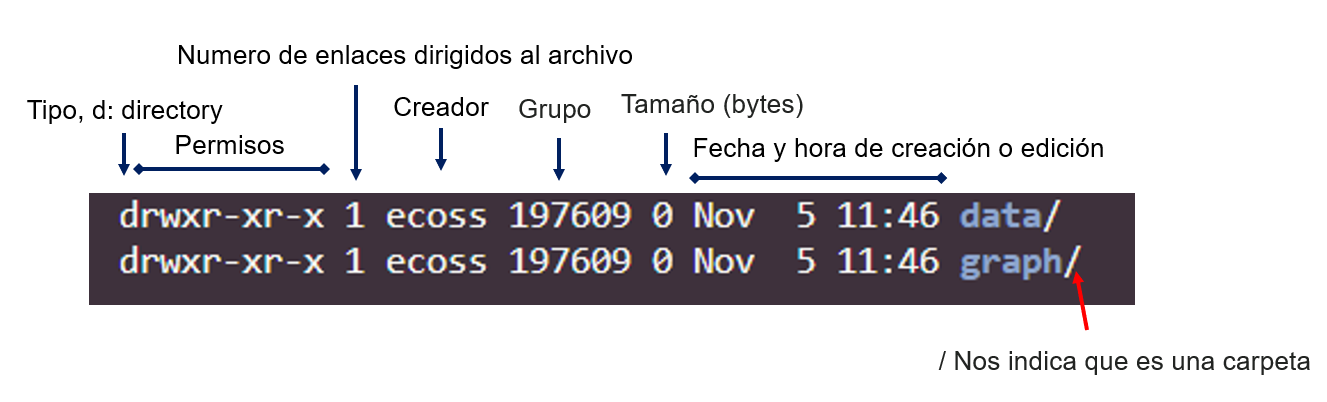
\includegraphics[keepaspectratio]{figures/ejemplo_datos.png}}}

\subsection{\texorpdfstring{\textbf{Permisos}}{Permisos}}\label{permisos}

Cada usuario tiene permisos diferentes cuando crea un archivo. Los
permisos pueden modificarse con \texttt{chmod}.

Los caracteres atribuidos a los permisos son:

\begin{itemize}
\item
  \texttt{r} : escritura (Read)
\item
  \texttt{w} : lectura (Write)
\item
  \texttt{x} : ejecución (eXecute)
\end{itemize}

En el siguiente ejemplo, el usuario cuenta con todos los permisos
activos, mientras que el grupo y otros tienen solo permisos de lectura y
ejecución.

\href{https://eveliacoss.github.io/RNAseq_classFEB2024/Presentaciones/Dia1_AspectosGenerales.html\#75}{\pandocbounded{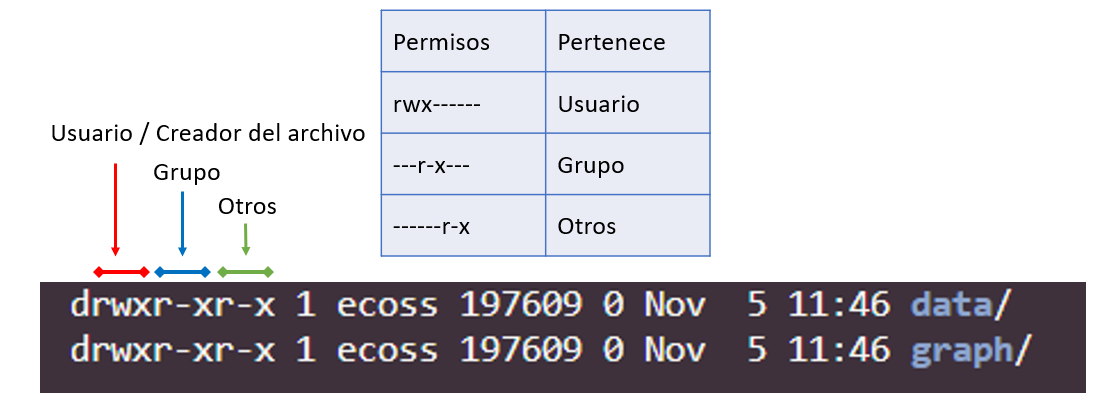
\includegraphics[keepaspectratio]{figures/permisos.png}}}

\section{\texorpdfstring{\textbf{\texttt{chmod}:} Cambiar
permisos}{chmod: Cambiar permisos}}\label{chmod-cambiar-permisos}

La representación octal de chmod es muy sencilla

\begin{itemize}
\item
  \texttt{r} = Lectura tiene el valor de 4
\item
  \texttt{w} = Escritura tiene el valor de 2
\item
  \texttt{x} = Ejecución tiene el valor de 1
\end{itemize}

{\def\LTcaptype{none} % do not increment counter
\begin{longtable}[]{@{}ccl@{}}
\toprule\noalign{}
Permisos & Valor & Significado \\
\midrule\noalign{}
\endhead
\bottomrule\noalign{}
\endlastfoot
rwx & 7 & Lectura, escritura y ejecución \\
rw- & 6 & Lectura, escritura \\
r-x & 5 & Lectura y ejecución \\
r-- & 4 & Lectura \\
-wx & 3 & Escritura y ejecución \\
-w- & 2 & Escritura \\
--x & 1 & Ejecución \\
--- & 0 & Sin permisos \\
\end{longtable}
}

Por lo tanto:

{\def\LTcaptype{none} % do not increment counter
\begin{longtable}[]{@{}ll@{}}
\toprule\noalign{}
Forma larga & Forma Octal \\
\midrule\noalign{}
\endhead
\bottomrule\noalign{}
\endlastfoot
\texttt{chmod\ u=rwx,g=rwx,o=rx} & \texttt{chmod\ 775} \\
\texttt{chmod\ u=rwx,g=rx,o=} & \texttt{chmod\ 760} \\
\texttt{chmod\ u=rw,g=r,o=r} & \texttt{chmod\ 644} \\
\texttt{chmod\ u=rw,g=r,o=} & \texttt{chmod\ 640} \\
\texttt{chmod\ u=rw,go=} & \texttt{chmod\ 600} \\
\texttt{chmod\ u=rwx,go=} & \texttt{chmod\ 700} \\
\end{longtable}
}

\section{Comprimir y descomprimir
archivos}\label{comprimir-y-descomprimir-archivos}

Los archivos pueden contener diversos tipos de extensiones, dependiendo
del objetivo será necesario descomprimirlos y en otros dejarlos
comprimidos para no abarcar tanto espacio en tu espacio de trabajo.~

{\def\LTcaptype{none} % do not increment counter
\begin{longtable}[]{@{}
  >{\raggedright\arraybackslash}p{(\linewidth - 4\tabcolsep) * \real{0.3333}}
  >{\raggedright\arraybackslash}p{(\linewidth - 4\tabcolsep) * \real{0.3333}}
  >{\raggedright\arraybackslash}p{(\linewidth - 4\tabcolsep) * \real{0.3333}}@{}}
\toprule\noalign{}
\begin{minipage}[b]{\linewidth}\raggedright
Tipo de archivo
\end{minipage} & \begin{minipage}[b]{\linewidth}\raggedright
Comprimir
\end{minipage} & \begin{minipage}[b]{\linewidth}\raggedright
Descomprimir
\end{minipage} \\
\midrule\noalign{}
\endhead
\bottomrule\noalign{}
\endlastfoot
Carpeta.tar & \texttt{tar\ -cvf\ carpeta.tar\ /dir/a/comprimir/carpeta}
& \texttt{tar\ -xvf\ carpeta.tar} \\
Carpeta.tar.gz &
\texttt{tar\ -czvf\ carpeta.tar.gz\ /carpeta/a/empaquetar/carpeta} &
\texttt{tar\ -zxvf\ carpeta.tar.gz} \\
Carpeta.gz & \texttt{gzip\ -9\ carpeta.gz\ carpeta/a/empaquetar/carpeta}
& \texttt{gunzip\ -kd\ carpeta.gz} \\
Carpeta.zip & \texttt{zip\ -r\ carpeta.zip\ carpeta} &
\texttt{unzip\ carpeta.zip} \\
\end{longtable}
}

\begin{tcolorbox}[enhanced jigsaw, arc=.35mm, bottomrule=.15mm, bottomtitle=1mm, breakable, colback=white, colbacktitle=quarto-callout-note-color!10!white, colframe=quarto-callout-note-color-frame, coltitle=black, left=2mm, leftrule=.75mm, opacityback=0, opacitybacktitle=0.6, rightrule=.15mm, title=\textcolor{quarto-callout-note-color}{\faInfo}\hspace{0.5em}{Ejercicio 2}, titlerule=0mm, toprule=.15mm, toptitle=1mm]

\begin{enumerate}
\def\labelenumi{\arabic{enumi}.}
\tightlist
\item
  Crea una carpeta llamada \texttt{respaldo}.
\end{enumerate}

\begin{Shaded}
\begin{Highlighting}[]
\FunctionTok{mkdir}\NormalTok{ respaldo}
\end{Highlighting}
\end{Shaded}

\begin{enumerate}
\def\labelenumi{\arabic{enumi}.}
\setcounter{enumi}{1}
\tightlist
\item
  Crea dentro de ella los archivos uno.txt, dos.txt y tres.txt. Usa el
  comando
\end{enumerate}

\begin{Shaded}
\begin{Highlighting}[]
\FunctionTok{touch}\NormalTok{ respaldo/uno.txt respaldo/dos.txt respaldo/tres.txt}
\end{Highlighting}
\end{Shaded}

\begin{enumerate}
\def\labelenumi{\arabic{enumi}.}
\setcounter{enumi}{2}
\tightlist
\item
  Configura los tres archivos con permisos \texttt{rw-r-\/-\/-\/-\/-}.
\end{enumerate}

Recuerda que:

\begin{itemize}
\tightlist
\item
  rw- = 6
\item
  r-- = 4
\item
  --- = 0
\end{itemize}

\begin{Shaded}
\begin{Highlighting}[]
\FunctionTok{chmod}\NormalTok{ 640 respaldo/}\PreprocessorTok{*}\NormalTok{.txt}
\end{Highlighting}
\end{Shaded}

Y comprueba que si se cambiaron los permisos con \texttt{l}s -l
respaldo`.

\begin{enumerate}
\def\labelenumi{\arabic{enumi}.}
\setcounter{enumi}{2}
\tightlist
\item
  Comprime la carpeta completa en un archivo llamado
  \texttt{respaldo.zip}
\end{enumerate}

\begin{Shaded}
\begin{Highlighting}[]
\FunctionTok{zip} \AttributeTok{{-}r}\NormalTok{ respaldo.zip respaldo/}
\end{Highlighting}
\end{Shaded}

La opción:

\begin{itemize}
\tightlist
\item
  \texttt{-r} → comprime de forma recursiva la carpeta y su contenido
\end{itemize}

\begin{enumerate}
\def\labelenumi{\arabic{enumi}.}
\setcounter{enumi}{3}
\tightlist
\item
  Elimina la carpeta \texttt{respaldo} (la que no esta comprimida).
\end{enumerate}

\begin{Shaded}
\begin{Highlighting}[]
\FunctionTok{rm} \AttributeTok{{-}r}\NormalTok{ respaldo}
\end{Highlighting}
\end{Shaded}

\begin{enumerate}
\def\labelenumi{\arabic{enumi}.}
\setcounter{enumi}{4}
\tightlist
\item
  Comprueba que la carpeta ya no existe.
\end{enumerate}

\begin{Shaded}
\begin{Highlighting}[]
\FunctionTok{ls}
\end{Highlighting}
\end{Shaded}

La carpeta respaldo ya no deberá aparecer, pero sí:
\texttt{respaldo.zip}.

\begin{enumerate}
\def\labelenumi{\arabic{enumi}.}
\setcounter{enumi}{5}
\tightlist
\item
  Recupera la carpeta utilizando \texttt{respaldo.zip}. Es decir,
  descomprime la carpeta \texttt{respaldo.zip}.
\end{enumerate}

\begin{Shaded}
\begin{Highlighting}[]
\FunctionTok{unzip}\NormalTok{ respaldo.zip}
\end{Highlighting}
\end{Shaded}

\begin{enumerate}
\def\labelenumi{\arabic{enumi}.}
\setcounter{enumi}{6}
\tightlist
\item
  Comprueba que los tres archivos fueron recuperados.
\end{enumerate}

\begin{Shaded}
\begin{Highlighting}[]
\FunctionTok{ls}\NormalTok{ respaldo}
\end{Highlighting}
\end{Shaded}

\begin{enumerate}
\def\labelenumi{\arabic{enumi}.}
\setcounter{enumi}{7}
\tightlist
\item
  Revisa sus permisos.
\end{enumerate}

\begin{Shaded}
\begin{Highlighting}[]
\FunctionTok{ls} \AttributeTok{{-}l}\NormalTok{ respaldo}
\end{Highlighting}
\end{Shaded}

\end{tcolorbox}

\section{Material suplementario}\label{material-suplementario-1}

\begin{itemize}
\tightlist
\item
  Software Carpentry.
  \href{https://swcarpentry.github.io/shell-novice-es/02-filedir.html}{La
  terminal de Unix}
\item
  RSG
  Ecuador.\href{https://rsg-ecuador.github.io/unix.bioinfo.rsgecuador/content/Curso_avanzado/02_Bash/1_bash.html}{GNU/Linux
  para bioinfomatica}
\item
  \href{https://github.com/raynamharris/Shell_Intro_for_Transcriptomics/tree/master}{Introduction
  to the Unix Shell for Transcriptomics}Tutorial.
\end{itemize}

\chapter{Caracteres, Strings y
Wildcards}\label{caracteres-strings-y-wildcards}

\begin{quote}
\textbf{Fecha:} 17 de septiembre, 2026
\end{quote}

\section{Estructura de declaración de variables en
bash}\label{estructura-de-declaraciuxf3n-de-variables-en-bash}

La estructura básica para declarar una variable en \texttt{bash} es:

\begin{verbatim}
nombre_variable=valor
\end{verbatim}

\subsection{Reglas importantes para nombres de
variables}\label{reglas-importantes-para-nombres-de-variables}

\begin{tcolorbox}[enhanced jigsaw, arc=.35mm, bottomrule=.15mm, breakable, colback=white, colframe=quarto-callout-important-color-frame, left=2mm, leftrule=.75mm, opacityback=0, rightrule=.15mm, toprule=.15mm]

\begin{itemize}
\item
  \textbf{Deben comenzar con una letra o guion bajo} (\texttt{\_})
\item
  \textbf{Pueden contener letras, números y guiones bajos}
\item
  \textbf{No pueden contener espacios} alrededor del signo \texttt{=}
\item
  \textbf{Son sensibles a mayúsculas y minúsculas} (edad ≠ EDAD)
\item
  \textbf{No se usan espacios} entre el nombre, el \texttt{=} y el valor
\end{itemize}

\end{tcolorbox}

\subsection{Ejemplos de declaración correcta e
incorrecta}\label{ejemplos-de-declaraciuxf3n-correcta-e-incorrecta}

\textbf{✅ Correcto:}

\begin{Shaded}
\begin{Highlighting}[]
\VariableTok{nombre}\OperatorTok{=}\StringTok{"Juan"}
\VariableTok{edad}\OperatorTok{=}\NormalTok{25}
\VariableTok{\_variable}\OperatorTok{=}\StringTok{"valor"}
\VariableTok{mi\_nombre}\OperatorTok{=}\StringTok{"Carlos"}
\end{Highlighting}
\end{Shaded}

\textbf{❌ Incorrecto:}

\begin{Shaded}
\begin{Highlighting}[]
\ExtensionTok{nombre}\NormalTok{ = }\StringTok{"Juan"}        \CommentTok{\# Espacios alrededor del =}
\ExtensionTok{2nombre=}\StringTok{"Juan"}         \CommentTok{\# Comienza con número}
\ExtensionTok{mi{-}nombre=}\StringTok{"Juan"}       \CommentTok{\# Guion en lugar de guion bajo}
\end{Highlighting}
\end{Shaded}

\section{Acceder a variables con \$}\label{acceder-a-variables-con}

Para \textbf{usar o acceder} al valor de una variable, debes anteponer
el símbolo \texttt{\$} al nombre:

\begin{Shaded}
\begin{Highlighting}[]
\VariableTok{nombre}\OperatorTok{=}\StringTok{"Juan"}
\BuiltInTok{echo} \VariableTok{$nombre}           \CommentTok{\# Output: Juan}
\BuiltInTok{echo} \StringTok{"Hola }\VariableTok{$nombre}\StringTok{"}    \CommentTok{\# Output: Hola Juan}
\end{Highlighting}
\end{Shaded}

\section{Tipos de comillas y su
comportamiento}\label{tipos-de-comillas-y-su-comportamiento}

\subsection{\texorpdfstring{Comillas dobles \texttt{"..."} - Expansión
de
variables}{Comillas dobles "..." - Expansión de variables}}\label{comillas-dobles-...---expansiuxf3n-de-variables}

Las comillas dobles \textbf{permiten la expansión de variables}. Esto
significa que el \texttt{\$} se interpreta como inicio de una variable:

\begin{Shaded}
\begin{Highlighting}[]
\VariableTok{nombre}\OperatorTok{=}\StringTok{"Juan"}
\BuiltInTok{echo} \StringTok{"Hola }\VariableTok{$nombre}\StringTok{"}    \CommentTok{\# Output: Hola Juan}
\end{Highlighting}
\end{Shaded}

Aquí, \texttt{\$nombre} se reemplaza por su valor \texttt{Juan}.

\subsection{\texorpdfstring{Comillas simples
\texttt{\textquotesingle{}...\textquotesingle{}} - Sin
expansión}{Comillas simples \textquotesingle...\textquotesingle{} - Sin expansión}}\label{comillas-simples-...---sin-expansiuxf3n}

Las comillas simples \textbf{tratan todo literalmente}. El \texttt{\$}
no se interpreta como variable:

\begin{Shaded}
\begin{Highlighting}[]
\VariableTok{nombre}\OperatorTok{=}\StringTok{"Juan"}
\BuiltInTok{echo} \StringTok{\textquotesingle{}Hola $nombre\textquotesingle{}}    \CommentTok{\# Output: Hola $nombre}
\end{Highlighting}
\end{Shaded}

Aquí, \texttt{\$nombre} se imprime tal cual, sin reemplazarse.

\subsection{Sin comillas - Expansión
directa}\label{sin-comillas---expansiuxf3n-directa}

Sin comillas, también se expanden las variables:

\begin{Shaded}
\begin{Highlighting}[]
\VariableTok{nombre}\OperatorTok{=}\StringTok{"Juan"}
\BuiltInTok{echo}\NormalTok{ Hola }\VariableTok{$nombre}      \CommentTok{\# Output: Hola Juan}
\end{Highlighting}
\end{Shaded}

\section{\texorpdfstring{\textbf{Caracteres}}{Caracteres}}\label{caracteres}

Los \texttt{caracteres} son unidades de información que se representan
con símbolos. Pueden ser de varios tipos como alfanuméricos, números
enteros, signos de puntuación. Varios caracteres son interpretados por
la shell de manera especial. Estos se llaman
\texttt{caracteres\ especiales}, claro, y permiten desarrollar alguna
lógica, dependiendo del contexto. Por ejemplo, algunos caracteres:
\texttt{@} \texttt{\#} \texttt{.} \texttt{?} \texttt{!} \texttt{,}
\texttt{/} \texttt{\textbackslash{}} \texttt{\textgreater{}}
\texttt{\textasciitilde{}} \texttt{a} \texttt{µ} \texttt{g} \texttt{§}
\texttt{R} \texttt{\textbar{}(pipe)}.

Cada carácter se asocia a una combinación diferente de teclas en el
teclado del computador. Representa un símbolo individual que puede ser:

\begin{itemize}
\tightlist
\item
  \textbf{Letras}: a, b, c, A, B, C, etc.
\item
  \textbf{Dígitos}: 0, 1, 2, 3, 4, 5, 6, 7, 8, 9
\item
  \textbf{Símbolos especiales}:
  \texttt{!,\ @,\ \#,\ \$,\ \%,\ \&,\ *,\ (,\ ),\ -,\ \_,\ +,\ =}, etc.
\item
  \textbf{Espacios en blanco}: espacios, tabulaciones, saltos de línea
\item
  \textbf{Caracteres de control}: caracteres invisibles que controlan el
  comportamiento (como el salto de línea)
\end{itemize}

\section{Metacaracteres}\label{metacaracteres}

\subsection{¿Qué son los
metacaracteres?}\label{quuxe9-son-los-metacaracteres}

Los \textbf{metacaracteres} son \textbf{caracteres especiales que tienen
un significado especial en bash}, en lugar de representar su valor
literal. \texttt{Bash} los interpreta como instrucciones o comandos, no
como texto normal.

\section{\texorpdfstring{\textbf{Strings}}{Strings}}\label{strings}

Los \texttt{strings} (o \textbf{cadena de texto}) son arreglos de
caracteres. Es decir, es una combinación de uno o más caracteres que
forman un texto.

\begin{verbatim}
"Hola"              → string de 4 caracteres
"Bash es genial"    → string de 14 caracteres (incluyendo espacios)
"12345"             → string de 5 caracteres
"!@#$%"             → string de 5 caracteres especiales
""                  → string vacío (0 caracteres)
\end{verbatim}

\subsection{Características de los strings en
bash}\label{caracteruxedsticas-de-los-strings-en-bash}

\subsection{Inmutabilidad en contexto de
asignación}\label{inmutabilidad-en-contexto-de-asignaciuxf3n}

Los strings en bash son \textbf{inmutables} en el sentido de que no
puedes modificar un carácter individual directamente. Debes reasignar
todo el string:

\begin{Shaded}
\begin{Highlighting}[]
\VariableTok{nombre}\OperatorTok{=}\StringTok{"Juan"}
\VariableTok{nombre}\OperatorTok{=}\StringTok{"Carlos"}    \CommentTok{\# Reasignación completa del string}
\BuiltInTok{echo} \VariableTok{$nombre}       \CommentTok{\# Output: Carlos}
\end{Highlighting}
\end{Shaded}

\subsection{Sensibilidad a mayúsculas y
minúsculas}\label{sensibilidad-a-mayuxfasculas-y-minuxfasculas}

Los strings \textbf{distinguen entre mayúsculas y minúsculas}. Dos
strings con diferente capitalización se consideran diferentes:

\begin{Shaded}
\begin{Highlighting}[]
\VariableTok{nombre}\OperatorTok{=}\StringTok{"juan"}
\VariableTok{NOMBRE}\OperatorTok{=}\StringTok{"JUAN"}
\BuiltInTok{echo} \VariableTok{$nombre}       \CommentTok{\# Output: juan}
\BuiltInTok{echo} \VariableTok{$NOMBRE}       \CommentTok{\# Output: JUAN}
\CommentTok{\# Son variables diferentes}
\end{Highlighting}
\end{Shaded}

\subsection{Pueden contener espacios en
blanco}\label{pueden-contener-espacios-en-blanco}

Los strings pueden incluir espacios, tabulaciones y saltos de línea.
Para preservarlos, debes usar comillas:

\begin{Shaded}
\begin{Highlighting}[]
\CommentTok{\# Con comillas (preserva espacios)}
\VariableTok{frase}\OperatorTok{=}\StringTok{"Hola mundo desde bash"}
\BuiltInTok{echo} \StringTok{"}\VariableTok{$frase}\StringTok{"}      \CommentTok{\# Output: Hola mundo desde bash}

\CommentTok{\# Sin comillas (los espacios se interpretan como separadores)}
\BuiltInTok{echo}\NormalTok{ Hola mundo    }\CommentTok{\# Output: Hola mundo (pero se trata como 2 argumentos)}
\end{Highlighting}
\end{Shaded}

\begin{tcolorbox}[enhanced jigsaw, arc=.35mm, bottomrule=.15mm, bottomtitle=1mm, breakable, colback=white, colbacktitle=quarto-callout-important-color!10!white, colframe=quarto-callout-important-color-frame, coltitle=black, left=2mm, leftrule=.75mm, opacityback=0, opacitybacktitle=0.6, rightrule=.15mm, title={¿Qué son los argumentos?}, titlerule=0mm, toprule=.15mm, toptitle=1mm]

Un \textbf{argumento} es un \textbf{valor o dato que se pasa a un
comando o programa} para que lo procese. Los argumentos son la forma en
que le das información a un comando sobre qué debe hacer.

\subsection{Estructura básica}\label{estructura-buxe1sica}

\begin{verbatim}
comando argumento1 argumento2 argumento3
\end{verbatim}

\subsection{Ejemplo sin comillas}\label{ejemplo-sin-comillas}

\begin{verbatim}
echo Hola mundo
\end{verbatim}

En este caso:

\begin{itemize}
\tightlist
\item
  \textbf{Comando}: \texttt{echo}
\item
  \textbf{Argumento 1}: \texttt{Hola}
\item
  \textbf{Argumento 2}: \texttt{mundo}
\end{itemize}

Bash pasa \textbf{dos argumentos} al comando \texttt{echo}, y
\texttt{echo} los imprime separados por un espacio.

\subsection{Ejemplo con comillas}\label{ejemplo-con-comillas}

\begin{verbatim}
echo "Hola mundo"
\end{verbatim}

En este caso:

\begin{itemize}
\tightlist
\item
  \textbf{Comando}: \texttt{echo}
\item
  \textbf{Argumento 1}: \texttt{Hola\ mundo} (un solo argumento)
\end{itemize}

\end{tcolorbox}

\subsection{Pueden estar vacíos}\label{pueden-estar-vacuxedos}

Un string puede no contener ningún carácter (string vacío):

\begin{Shaded}
\begin{Highlighting}[]
\VariableTok{variable}\OperatorTok{=}\StringTok{""}
\BuiltInTok{echo} \StringTok{"La variable está vacía: \textquotesingle{}}\VariableTok{$variable}\StringTok{\textquotesingle{}"}  \CommentTok{\# Output: La variable está vacía: \textquotesingle{}\textquotesingle{}}
\end{Highlighting}
\end{Shaded}

\subsection{Concatenación automática /
Unión}\label{concatenaciuxf3n-automuxe1tica-uniuxf3n}

Bash permite concatenar strings simplemente colocándolos uno al lado del
otro:

\begin{Shaded}
\begin{Highlighting}[]
\VariableTok{nombre}\OperatorTok{=}\StringTok{"Juan"}
\VariableTok{apellido}\OperatorTok{=}\StringTok{"Pérez"}

\CommentTok{\# Concatenación sin espacios}
\VariableTok{completo}\OperatorTok{=}\VariableTok{$nombre$apellido}
\BuiltInTok{echo} \VariableTok{$completo}     \CommentTok{\# Output: JuanPérez}

\CommentTok{\# Concatenación con espacios}
\VariableTok{completo}\OperatorTok{=}\StringTok{"}\VariableTok{$nombre}\StringTok{ }\VariableTok{$apellido}\StringTok{"}
\BuiltInTok{echo} \VariableTok{$completo}     \CommentTok{\# Output: Juan Pérez}

\CommentTok{\# Concatenación con variables y texto literal}
\VariableTok{mensaje}\OperatorTok{=}\StringTok{"Hola, }\VariableTok{$nombre}\StringTok{"}
\BuiltInTok{echo} \VariableTok{$mensaje}      \CommentTok{\# Output: Hola, Juan}
\end{Highlighting}
\end{Shaded}

\subsection{Longitud de strings}\label{longitud-de-strings}

Puedes obtener la longitud de un string usando
\texttt{\$\{\#variable\}}:

\begin{tcolorbox}[enhanced jigsaw, arc=.35mm, bottomrule=.15mm, bottomtitle=1mm, breakable, colback=white, colbacktitle=quarto-callout-important-color!10!white, colframe=quarto-callout-important-color-frame, coltitle=black, left=2mm, leftrule=.75mm, opacityback=0, opacitybacktitle=0.6, rightrule=.15mm, title={Desglose de la sintaxis \texttt{\$\{\#variable\}}}, titlerule=0mm, toprule=.15mm, toptitle=1mm]

\begin{itemize}
\tightlist
\item
  \texttt{\$\{\ \}} → Delimitadores para expansión de variables en bash
\item
  \texttt{\#} → Operador que significa ``obtener la longitud''
\item
  \texttt{variable} → El nombre de la variable cuya longitud quieres
  obtener
\end{itemize}

\end{tcolorbox}

Ejemplos:

\begin{Shaded}
\begin{Highlighting}[]
\VariableTok{nombre}\OperatorTok{=}\StringTok{"Juan"}
\VariableTok{longitud}\OperatorTok{=}\VariableTok{$\{}\OperatorTok{\#}\VariableTok{nombre\}}
\BuiltInTok{echo} \StringTok{"La longitud es: }\VariableTok{$longitud}\StringTok{"}  \CommentTok{\# Output: La longitud es: 4}

\CommentTok{\# Ejemplo con string más largo}
\VariableTok{frase}\OperatorTok{=}\StringTok{"Bash es genial"}
\BuiltInTok{echo} \VariableTok{$\{}\OperatorTok{\#}\VariableTok{frase\}}     \CommentTok{\# Output: 14 (incluyendo espacios)}
\end{Highlighting}
\end{Shaded}

\subsection{Extracción de subcadenas}\label{extracciuxf3n-de-subcadenas}

Puedes extraer una parte de un string usando
\texttt{\$\{variable:inicio:longitud\}}:

\begin{tcolorbox}[enhanced jigsaw, arc=.35mm, bottomrule=.15mm, bottomtitle=1mm, breakable, colback=white, colbacktitle=quarto-callout-important-color!10!white, colframe=quarto-callout-important-color-frame, coltitle=black, left=2mm, leftrule=.75mm, opacityback=0, opacitybacktitle=0.6, rightrule=.15mm, title={Desglose de la sintaxis \texttt{\$\{variable:inicio:longitud\}}}, titlerule=0mm, toprule=.15mm, toptitle=1mm]

\begin{itemize}
\tightlist
\item
  \texttt{\$\{\ \}} → Delimitadores para expansión de variables en bash
\item
  \texttt{variable} → El nombre de la variable de la cual extraerás
  caracteres
\item
  \texttt{:inicio} → La posición donde comienza la extracción (comienza
  en 0)
\item
  \texttt{:longitud} → Cuántos caracteres quieres extraer
\end{itemize}

\end{tcolorbox}

Ejemplos:

\begin{Shaded}
\begin{Highlighting}[]
\VariableTok{nombre}\OperatorTok{=}\StringTok{"Juan"}

\CommentTok{\# Extraer desde posición 0, 2 caracteres}
\BuiltInTok{echo} \VariableTok{$\{nombre}\OperatorTok{:}\DecValTok{0}\OperatorTok{:}\DecValTok{2}\VariableTok{\}}    \CommentTok{\# Output: Ju}

\CommentTok{\# Extraer desde posición 1, 2 caracteres}
\BuiltInTok{echo} \VariableTok{$\{nombre}\OperatorTok{:}\DecValTok{1}\OperatorTok{:}\DecValTok{2}\VariableTok{\}}    \CommentTok{\# Output: ua}

\CommentTok{\# Extraer desde posición 2 hasta el final}
\BuiltInTok{echo} \VariableTok{$\{nombre}\OperatorTok{:}\DecValTok{2}\VariableTok{\}}      \CommentTok{\# Output: an}
\end{Highlighting}
\end{Shaded}

\subsection{Sustitución de patrones}\label{sustituciuxf3n-de-patrones}

Puedes reemplazar partes de un string usando
\texttt{\$\{variable/patron/reemplazo\}}:

\begin{Shaded}
\begin{Highlighting}[]
\VariableTok{frase}\OperatorTok{=}\StringTok{"Hola mundo mundo"}

\CommentTok{\# Reemplazar la primera ocurrencia}
\BuiltInTok{echo} \VariableTok{$\{frase}\OperatorTok{/}\SpecialStringTok{mundo}\OperatorTok{/}\NormalTok{bash}\VariableTok{\}}      \CommentTok{\# Output: Hola bash mundo}

\CommentTok{\# Reemplazar todas las ocurrencias (con //)}
\BuiltInTok{echo} \VariableTok{$\{frase}\OperatorTok{//}\SpecialStringTok{mundo}\OperatorTok{/}\NormalTok{bash}\VariableTok{\}}     \CommentTok{\# Output: Hola bash bash}
\end{Highlighting}
\end{Shaded}

\subsection{Eliminación de patrones}\label{eliminaciuxf3n-de-patrones}

Puedes eliminar partes de un string:

\begin{Shaded}
\begin{Highlighting}[]
\VariableTok{nombre}\OperatorTok{=}\StringTok{"Juan.txt"}

\CommentTok{\# Eliminar desde el final hasta el patrón}
\BuiltInTok{echo} \VariableTok{$\{nombre}\OperatorTok{\%}\NormalTok{.txt}\VariableTok{\}}           \CommentTok{\# Output: Juan}

\CommentTok{\# Eliminar desde el inicio hasta el patrón}
\BuiltInTok{echo} \VariableTok{$\{nombre}\OperatorTok{\#}\NormalTok{Juan.}\VariableTok{\}}          \CommentTok{\# Output: txt}
\end{Highlighting}
\end{Shaded}

\subsection{Conversión a mayúsculas y
minúsculas}\label{conversiuxf3n-a-mayuxfasculas-y-minuxfasculas}

Bash permite convertir strings a mayúsculas o minúsculas (en versiones
4.0+):

\begin{Shaded}
\begin{Highlighting}[]
\VariableTok{nombre}\OperatorTok{=}\StringTok{"Juan"}

\CommentTok{\# Convertir a mayúsculas}
\BuiltInTok{echo} \VariableTok{$\{nombre}\OperatorTok{\^{}\^{}}\VariableTok{\}}              \CommentTok{\# Output: JUAN}

\CommentTok{\# Convertir a minúsculas}
\BuiltInTok{echo} \VariableTok{$\{nombre}\OperatorTok{,,}\VariableTok{\}}              \CommentTok{\# Output: juan}

\CommentTok{\# Convertir solo el primer carácter a mayúscula}
\BuiltInTok{echo} \VariableTok{$\{nombre}\OperatorTok{\^{}}\VariableTok{\}}               \CommentTok{\# Output: Juan}
\end{Highlighting}
\end{Shaded}

\subsection{Comparación de strings}\label{comparaciuxf3n-de-strings}

Puedes comparar strings usando operadores:

\begin{Shaded}
\begin{Highlighting}[]
\VariableTok{nombre1}\OperatorTok{=}\StringTok{"Juan"}
\VariableTok{nombre2}\OperatorTok{=}\StringTok{"Juan"}
\VariableTok{nombre3}\OperatorTok{=}\StringTok{"Carlos"}

\CommentTok{\# Igualdad}
\BuiltInTok{echo} \StringTok{"}\VariableTok{$nombre1}\StringTok{ = }\VariableTok{$nombre2}\StringTok{"}    \CommentTok{\# Output: Juan = Juan}

\CommentTok{\# Desigualdad}
\BuiltInTok{echo} \StringTok{"}\VariableTok{$nombre1}\StringTok{ != }\VariableTok{$nombre3}\StringTok{"}   \CommentTok{\# Output: Juan != Carlos}
\end{Highlighting}
\end{Shaded}

\subsection{Expansión de variables dentro de
strings}\label{expansiuxf3n-de-variables-dentro-de-strings}

La expansión de variables ocurre dentro de comillas dobles pero no en
comillas simples:

\begin{Shaded}
\begin{Highlighting}[]
\VariableTok{nombre}\OperatorTok{=}\StringTok{"Juan"}

\CommentTok{\# Con comillas dobles (expansión)}
\BuiltInTok{echo} \StringTok{"Hola }\VariableTok{$nombre}\StringTok{"}           \CommentTok{\# Output: Hola Juan}

\CommentTok{\# Con comillas simples (sin expansión)}
\BuiltInTok{echo} \StringTok{\textquotesingle{}Hola $nombre\textquotesingle{}}           \CommentTok{\# Output: Hola $nombre}

\CommentTok{\# Sin comillas (expansión)}
\BuiltInTok{echo}\NormalTok{ Hola }\VariableTok{$nombre}             \CommentTok{\# Output: Hola Juan}
\end{Highlighting}
\end{Shaded}

\subsection{Caracteres especiales y
escape}\label{caracteres-especiales-y-escape}

Algunos caracteres tienen significado especial en bash. Puedes
escaparlos con \texttt{\textbackslash{}}:

\begin{Shaded}
\begin{Highlighting}[]
\CommentTok{\# Caracteres especiales}
\BuiltInTok{echo} \StringTok{"Precio: }\DataTypeTok{\textbackslash{}$}\StringTok{100"}          \CommentTok{\# Output: Precio: $100}
\BuiltInTok{echo} \StringTok{"Comilla: }\DataTypeTok{\textbackslash{}"}\StringTok{Hola}\DataTypeTok{\textbackslash{}"}\StringTok{"}      \CommentTok{\# Output: Comilla: "Hola"}
\BuiltInTok{echo} \StringTok{"Barra invertida: }\DataTypeTok{\textbackslash{}\textbackslash{}}\StringTok{"}    \CommentTok{\# Output: Barra invertida: \textbackslash{}}

\CommentTok{\# Saltos de línea}
\BuiltInTok{echo} \AttributeTok{{-}e} \StringTok{"Línea 1\textbackslash{}nLínea 2"}    \CommentTok{\# Output: Línea 1}
                              \CommentTok{\#         Línea 2}
\end{Highlighting}
\end{Shaded}

\begin{tcolorbox}[enhanced jigsaw, arc=.35mm, bottomrule=.15mm, bottomtitle=1mm, breakable, colback=white, colbacktitle=quarto-callout-tip-color!10!white, colframe=quarto-callout-tip-color-frame, coltitle=black, left=2mm, leftrule=.75mm, opacityback=0, opacitybacktitle=0.6, rightrule=.15mm, title={\textbf{¿Qué es \texttt{\textbackslash{}n}?}}, titlerule=0mm, toprule=.15mm, toptitle=1mm]

\texttt{\textbackslash{}n} es una \textbf{secuencia de escape} que
representa un \textbf{salto de línea o enter}. Es decir, le dice al
programa que cree una nueva línea.

\begin{itemize}
\tightlist
\item
  \texttt{\textbackslash{}} → Carácter de escape (indica que lo
  siguiente tiene un significado especial)
\item
  \texttt{n} → Significa ``newline'' (nueva línea en inglés)
\end{itemize}

\end{tcolorbox}

\begin{tcolorbox}[enhanced jigsaw, arc=.35mm, bottomrule=.15mm, bottomtitle=1mm, breakable, colback=white, colbacktitle=quarto-callout-important-color!10!white, colframe=quarto-callout-important-color-frame, coltitle=black, left=2mm, leftrule=.75mm, opacityback=0, opacitybacktitle=0.6, rightrule=.15mm, title={¿Por qué necesitas \texttt{-e} en \texttt{echo} al usar
\texttt{\textbackslash{}n}?}, titlerule=0mm, toprule=.15mm, toptitle=1mm]

El comando \texttt{echo} \textbf{no interpreta}
\texttt{\textbackslash{}n} por defecto. Necesitas la opción \texttt{-e}
para que bash entienda que \texttt{\textbackslash{}n} significa un salto
de línea:

\begin{Shaded}
\begin{Highlighting}[]
\CommentTok{\# Sin {-}e: imprime \textbackslash{}n literalmente}
\BuiltInTok{echo} \StringTok{"Línea 1\textbackslash{}nLínea 2"}
\CommentTok{\# Output: Línea 1\textbackslash{}nLínea 2}

\CommentTok{\# Con {-}e: interpreta \textbackslash{}n como salto de línea}
\BuiltInTok{echo} \AttributeTok{{-}e} \StringTok{"Línea 1\textbackslash{}nLínea 2"}
\CommentTok{\# Output: Línea 1}
\CommentTok{\#         Línea 2}
\end{Highlighting}
\end{Shaded}

\end{tcolorbox}

\subsubsection{Otras secuencias de escape comunes
📌}\label{otras-secuencias-de-escape-comunes}

Además de \texttt{\textbackslash{}n}, existen otras secuencias de escape
útiles:

\begin{Shaded}
\begin{Highlighting}[]
\CommentTok{\# \textbackslash{}t = tabulación (espacios)}
\BuiltInTok{echo} \AttributeTok{{-}e} \StringTok{"Nombre:\textbackslash{}tJuan"}
\CommentTok{\# Output: Nombre:    Juan}

\CommentTok{\# \textbackslash{}\textbackslash{} = barra invertida literal}
\BuiltInTok{echo} \AttributeTok{{-}e} \StringTok{"Ruta: C:}\DataTypeTok{\textbackslash{}\textbackslash{}}\StringTok{Users}\DataTypeTok{\textbackslash{}\textbackslash{}}\StringTok{Juan"}
\CommentTok{\# Output: Ruta: C:\textbackslash{}Users\textbackslash{}Juan}

\CommentTok{\# \textbackslash{}" = comilla doble literal}
\BuiltInTok{echo} \AttributeTok{{-}e} \StringTok{"Dice: }\DataTypeTok{\textbackslash{}"}\StringTok{Hola}\DataTypeTok{\textbackslash{}"}\StringTok{"}
\CommentTok{\# Output: Dice: "Hola"}
\end{Highlighting}
\end{Shaded}

\subsection{Strings multilínea}\label{strings-multiluxednea}

Puedes crear strings que abarquen múltiples líneas:

\begin{Shaded}
\begin{Highlighting}[]
\CommentTok{\# Usando comillas dobles}
\VariableTok{texto}\OperatorTok{=}\StringTok{"Primera línea}
\StringTok{Segunda línea}
\StringTok{Tercera línea"}
\BuiltInTok{echo} \StringTok{"}\VariableTok{$texto}\StringTok{"}

\CommentTok{\# Usando $\textquotesingle{}...\textquotesingle{} (permite secuencias de escape)}
\VariableTok{texto}\OperatorTok{=}\StringTok{$\textquotesingle{}Primera línea}\DataTypeTok{\textbackslash{}n}\StringTok{Segunda línea}\DataTypeTok{\textbackslash{}n}\StringTok{Tercera línea\textquotesingle{}}
\BuiltInTok{echo} \StringTok{"}\VariableTok{$texto}\StringTok{"}
\end{Highlighting}
\end{Shaded}

\textbf{Resumen 🎯}

\begin{itemize}
\tightlist
\item
  \textbf{Saltos de línea literales} (Enter real en el código): No
  necesitan \texttt{-e} ni \texttt{\textbackslash{}n}
\item
  \textbf{Secuencias de escape \texttt{\textbackslash{}n}}: Necesitan
  \texttt{-e} o \texttt{\$\textquotesingle{}...\textquotesingle{}} para
  interpretarse
\end{itemize}

\section{\texorpdfstring{\textbf{Wildcards}}{Wildcards}}\label{wildcards}

Los \texttt{wildcards} (comodines) o \texttt{wild\ characters} son
símbolos utilizados para representar uno o más caracteres. Se pueden
utilizar con otros comandos para facilitar el procesamiento o búsqueda
de archivos, directorios y datos en general.

{\def\LTcaptype{none} % do not increment counter
\begin{longtable}[]{@{}
  >{\raggedright\arraybackslash}p{(\linewidth - 6\tabcolsep) * \real{0.2500}}
  >{\raggedright\arraybackslash}p{(\linewidth - 6\tabcolsep) * \real{0.2500}}
  >{\raggedright\arraybackslash}p{(\linewidth - 6\tabcolsep) * \real{0.2500}}
  >{\raggedright\arraybackslash}p{(\linewidth - 6\tabcolsep) * \real{0.2500}}@{}}
\toprule\noalign{}
\begin{minipage}[b]{\linewidth}\raggedright
Wildcard
\end{minipage} & \begin{minipage}[b]{\linewidth}\raggedright
Significa
\end{minipage} & \begin{minipage}[b]{\linewidth}\raggedright
Ejemplo
\end{minipage} & \begin{minipage}[b]{\linewidth}\raggedright
Coincide con
\end{minipage} \\
\midrule\noalign{}
\endhead
\bottomrule\noalign{}
\endlastfoot
\texttt{*} & Cero o más caracteres & \texttt{*.txt} & archivo.txt,
doc.txt, a.txt \\
\texttt{?} & Exactamente 1 carácter & \texttt{archivo?.txt} &
archivo1.txt, archivo2.txt \\
\texttt{{[}\ {]}} & Un carácter del conjunto & \texttt{{[}abc{]}*} &
archivo.txt, buscador.log, carpeta \\
\texttt{{[}!...{]}} & Un carácter NO en el conjunto &
\texttt{{[}!0-9{]}*} & archivo.txt (NO comienza con número) \\
\texttt{{[}a-z{]}} & Rango de caracteres & \texttt{{[}a-z{]}*} &
archivo.txt (comienza con minúscula) \\
\texttt{{[}0-9{]}} & Rango de números & \texttt{*{[}0-9{]}} & archivo1,
test2 \\
\end{longtable}
}

\begin{tcolorbox}[enhanced jigsaw, arc=.35mm, bottomrule=.15mm, bottomtitle=1mm, breakable, colback=white, colbacktitle=quarto-callout-important-color!10!white, colframe=quarto-callout-important-color-frame, coltitle=black, left=2mm, leftrule=.75mm, opacityback=0, opacitybacktitle=0.6, rightrule=.15mm, title=\textcolor{quarto-callout-important-color}{\faExclamation}\hspace{0.5em}{Importante}, titlerule=0mm, toprule=.15mm, toptitle=1mm]

El wildcard más usado es \texttt{*} porque es muy versátil.

\end{tcolorbox}

\begin{tcolorbox}[enhanced jigsaw, arc=.35mm, bottomrule=.15mm, bottomtitle=1mm, breakable, colback=white, colbacktitle=quarto-callout-note-color!10!white, colframe=quarto-callout-note-color-frame, coltitle=black, left=2mm, leftrule=.75mm, opacityback=0, opacitybacktitle=0.6, rightrule=.15mm, title=\textcolor{quarto-callout-note-color}{\faInfo}\hspace{0.5em}{Ejercicio 3}, titlerule=0mm, toprule=.15mm, toptitle=1mm]

El wildcard \texttt{*} me permitiría encontrar todos los archivos en una
carpeta que tengan la palabra \texttt{TESIS} en ellos. Primero crea la
carpeta:

\begin{Shaded}
\begin{Highlighting}[]
\FunctionTok{mkdir}\NormalTok{ taller\_unix}
\end{Highlighting}
\end{Shaded}

Después, debemos generar estos archivos:

\begin{Shaded}
\begin{Highlighting}[]
\BuiltInTok{cd}\NormalTok{ taller\_unix/}
\FunctionTok{touch}\NormalTok{ MI\_TESIS.tex MI\_TESIS\_tutor2.tex TESIS.tex TESIS\_YA\_ACABATE.tex TESIS\_finaaaaal.tex TESIS\_final.tex TESIS\_tutor1.tex TESIS\_tutor2.tex a\_reporte\_01.txt b\_reporte\_02.txt c\_reporte\_03.txt z\_reporte\_30.txt }
\end{Highlighting}
\end{Shaded}

\begin{enumerate}
\def\labelenumi{\arabic{enumi}.}
\item
  Enlista todos los archivos que comiencen con ``\texttt{TESIS}''.
\item
  Enlista todos los archivos que terminen con el string
  ``\texttt{.tex}''
\item
  Buscar todos los archivos contengan la palabra ``\texttt{TESIS"} pero
  con 3 caracteres desconocidos antes.
\item
  Buscar los archivos que terminen con el número 1 o 2 en su nombre
  antes de la extensión del archivo (\texttt{.tex}).
\item
  Encontrar los archivos que terminen en dos números del 1 al 3 y del 0
  al 2 antes del formato del archivo (\texttt{.txt}).
\item
  Encontrar todos los archivos con este formato
  \texttt{?\_reporte\_{[}0-3{]}{[}0-3{]}.txt}
\item
  Encontrar todos los archivos que contengan por \texttt{a} o
  \texttt{z}.
\item
  Borramos todos estor archivos que terminen en ``.txt'' y ``.tex''

  \begin{quote}
  \textbf{Solución}

\begin{Shaded}
\begin{Highlighting}[]
\ExtensionTok{1.}\NormalTok{ ls }\AttributeTok{{-}l}\NormalTok{ TESIS}\PreprocessorTok{*}
\ExtensionTok{2.}\NormalTok{ ls }\AttributeTok{{-}l} \PreprocessorTok{*}\NormalTok{.tex}
\ExtensionTok{3.}\NormalTok{ ls }\AttributeTok{{-}l} \PreprocessorTok{???}\NormalTok{TESIS}\PreprocessorTok{*}
\ExtensionTok{4.}\NormalTok{ ls }\AttributeTok{{-}l} \PreprocessorTok{*[}\SpecialStringTok{1}\PreprocessorTok{{-}}\SpecialStringTok{2}\PreprocessorTok{]}\NormalTok{.tex}
\ExtensionTok{5.}\NormalTok{ ls }\AttributeTok{{-}l} \PreprocessorTok{*[}\SpecialStringTok{1}\PreprocessorTok{{-}}\SpecialStringTok{3}\PreprocessorTok{][}\SpecialStringTok{0}\PreprocessorTok{{-}}\SpecialStringTok{2}\PreprocessorTok{]}\NormalTok{.txt}
\ExtensionTok{6.}\NormalTok{ ls }\AttributeTok{{-}l} \PreprocessorTok{?}\NormalTok{\_reporte\_}\PreprocessorTok{[}\SpecialStringTok{0}\PreprocessorTok{{-}}\SpecialStringTok{3}\PreprocessorTok{][}\SpecialStringTok{0}\PreprocessorTok{{-}}\SpecialStringTok{3}\PreprocessorTok{]}\NormalTok{.txt}
\ExtensionTok{7.}\NormalTok{ ls }\AttributeTok{{-}l} \PreprocessorTok{*[}\SpecialStringTok{az}\PreprocessorTok{]*}
\ExtensionTok{8.}\NormalTok{ rm }\PreprocessorTok{*}\NormalTok{.tex }\PreprocessorTok{*}\NormalTok{.txt}
\end{Highlighting}
\end{Shaded}
  \end{quote}
\end{enumerate}

\end{tcolorbox}

\section{Material suplementario}\label{material-suplementario-2}

\begin{itemize}
\tightlist
\item
  RSG Ecuador.
  \href{https://rsg-ecuador.github.io/unix.bioinfo.rsgecuador/content/Curso_avanzado/02_Bash/1_bash.html}{Scripts
  en Bash}
\item
  RSG Ecuador.
  \href{https://rsg-ecuador.github.io/unix.bioinfo.rsgecuador/content/Curso_basico/03_Manejo_terminal/5_wildcards.html}{Wildcards
  y Streams}
\item
  RSG Ecuador.
  \href{https://rsg-ecuador.github.io/unix.bioinfo.rsgecuador/content/Curso_basico/04_Procesamiento_ficheros_regex_pipes/3_Expresiones_regulares.html}{Expresiones
  regulares (\emph{regex})}
\item
  \href{https://pressbooks.senecapolytechnic.ca/uli101/chapter/wildcard-selection-in-bash/}{Wildcard
  Selection in Bash}
\item
  \href{https://twiki.org/cgi-bin/view/Codev/TWikiPresentation2017x06x01Regex}{Expresiones
  regulares}
\end{itemize}

\chapter{Expresiones regulares
(REGEX)}\label{expresiones-regulares-regex}

\begin{quote}
\textbf{Fecha:} 17 de septiembre, 2026
\end{quote}

Las \textbf{expresiones regulares} (o \textbf{REGEX}) son
\textbf{patrones de texto que describen un conjunto de strings} (cadenas
de caracteres). Te permiten buscar, validar y procesar texto de manera
flexible y poderosa.

\begin{tcolorbox}[enhanced jigsaw, arc=.35mm, bottomrule=.15mm, breakable, colback=white, colframe=quarto-callout-tip-color-frame, left=2mm, leftrule=.75mm, opacityback=0, rightrule=.15mm, toprule=.15mm]

\textbf{Idea principal 🎯:}

Una expresión regular es como un \textbf{patrón de búsqueda avanzado}
que te permite encontrar texto que coincida con reglas específicas, sin
necesidad de escribir el texto exacto.

\end{tcolorbox}

\textbf{Estructura de una expresión regular}

\begin{verbatim}
patrón = [caracteres] [metacaracteres] [cuantificadores]
\end{verbatim}

Estructura básica de grep

\begin{verbatim}
grep [opciones] "patrón" archivo.txt
\end{verbatim}

Componentes:

\begin{itemize}
\tightlist
\item
  \texttt{grep} = Comando
\item
  \texttt{{[}opciones{]}} = Modificadores del comportamiento (opcional)
\item
  \texttt{"patrón"} = La expresión regular a buscar
\item
  \texttt{archivo.txt} = El archivo donde buscar
\end{itemize}

\textbf{1. Caracteres literales}

Son caracteres normales que se buscan tal cual.

\begin{Shaded}
\begin{Highlighting}[]
\FunctionTok{grep} \StringTok{"hola"}\NormalTok{ archivo.txt}
\CommentTok{\# Busca la palabra "hola" exactamente}
\end{Highlighting}
\end{Shaded}

\textbf{2. Metacaracteres en REGEX}

Son caracteres especiales que tienen significado especial.

\begin{Shaded}
\begin{Highlighting}[]
\FunctionTok{grep} \StringTok{"h.la"}\NormalTok{ archivo.txt}
\CommentTok{\# Busca "hala", "hila", "hola", "hula", etc.}
\end{Highlighting}
\end{Shaded}

\textbf{3. Cuantificadores}

Especifican cuántas veces debe repetirse un patrón.

\begin{Shaded}
\begin{Highlighting}[]
\FunctionTok{grep} \StringTok{"ho*la"}\NormalTok{ archivo.txt}
\CommentTok{\# Busca "hla", "hola", "hoola", "hooola", etc.}
\end{Highlighting}
\end{Shaded}

\section{Diferencia: Wildcards vs REGEX
🔄}\label{diferencia-wildcards-vs-regex}

\subsubsection{Wildcards (en bash)}\label{wildcards-en-bash}

\begin{Shaded}
\begin{Highlighting}[]
\CommentTok{\# Buscar archivos}
\FunctionTok{ls} \PreprocessorTok{*}\NormalTok{.txt           }\CommentTok{\# Expande a archivos reales}
\FunctionTok{ls} \PreprocessorTok{[}\SpecialStringTok{abc}\PreprocessorTok{]*}          \CommentTok{\# Expande a archivos que comienzan con a, b o c}
\end{Highlighting}
\end{Shaded}

\textbf{Contexto}: Sistema de archivos

\subsubsection{REGEX (en comandos)}\label{regex-en-comandos}

\begin{Shaded}
\begin{Highlighting}[]
\CommentTok{\# Buscar en contenido de archivos}
\FunctionTok{grep} \StringTok{".*\textbackslash{}.txt$"}\NormalTok{ archivo.txt    }\CommentTok{\# Busca líneas que terminan en .txt}
\FunctionTok{grep} \StringTok{"[abc]"}\NormalTok{ archivo.txt       }\CommentTok{\# Busca líneas que contienen a, b o c}
\end{Highlighting}
\end{Shaded}

\textbf{Contexto}: Contenido de texto

\section{Operadores de redirección de datos
I/O}\label{operadores-de-redirecciuxf3n-de-datos-io}

Usualmente cuando trabajamos con datos, es necesario pasar el resultado
de un comando a otro para hacer un procesamiento de datos apilado, como
en un algortimo. Un \texttt{stream} o \texttt{corriente} esta hecha de
datos. Es una corriente de datos. Un ejemplo muy familiar es el teclado
y la pantalla. El teclado tiene una interfaz en donde por cada tecla
presionada, un caracter se guarda en un archivo. Se dice entonces que es
una \texttt{corriente\ de\ \ entrada}. Cuando la pantalla nos muestra lo
que estamos escribiendo entonces la data sale hacia nosotros y eso
convierte a la pantalla en una \texttt{corriente\ de\ salida}. Los
dispositivos que hacen este tipo de transmisión de datos se llaman
dispositivos \texttt{I/O} (input y output). Los operadores que se
encargan de esto se conocen como \texttt{operadores\ de\ redirección}.
Tres importantes son:

{\def\LTcaptype{none} % do not increment counter
\begin{longtable}[]{@{}
  >{\raggedright\arraybackslash}p{(\linewidth - 2\tabcolsep) * \real{0.5000}}
  >{\raggedright\arraybackslash}p{(\linewidth - 2\tabcolsep) * \real{0.5000}}@{}}
\toprule\noalign{}
\begin{minipage}[b]{\linewidth}\raggedright
\textbf{Comando}
\end{minipage} & \begin{minipage}[b]{\linewidth}\raggedright
\textbf{Función}
\end{minipage} \\
\midrule\noalign{}
\endhead
\bottomrule\noalign{}
\endlastfoot
\texttt{\textgreater{}} & Stream de \textbf{salida de datos}. Sobre
escribre sobre un archivo. \\
\texttt{\textgreater{}\textgreater{}} & Stream de salida de datos.
Adjunta \textbf{nueva salida a datos preexistentes en un archivo.} \\
\texttt{\textless{}} & Stream de \textbf{entrada de datos.} Recibe datos
para procesamiento con algun comando. \\
\end{longtable}
}

\begin{tcolorbox}[enhanced jigsaw, arc=.35mm, bottomrule=.15mm, bottomtitle=1mm, breakable, colback=white, colbacktitle=quarto-callout-note-color!10!white, colframe=quarto-callout-note-color-frame, coltitle=black, left=2mm, leftrule=.75mm, opacityback=0, opacitybacktitle=0.6, rightrule=.15mm, title=\textcolor{quarto-callout-note-color}{\faInfo}\hspace{0.5em}{Ejercicio 4}, titlerule=0mm, toprule=.15mm, toptitle=1mm]

\begin{enumerate}
\def\labelenumi{\arabic{enumi}.}
\item
  Crea el archivo \texttt{temas\_matematicas.txt} e imprime su contenido
  empleando los siguientes comandos:

\begin{Shaded}
\begin{Highlighting}[]
\BuiltInTok{echo} \AttributeTok{{-}e} \StringTok{"Álgebra\textbackslash{}nGeometría\textbackslash{}nCálculo\textbackslash{}nEstadística\textbackslash{}nProbabilidad\textbackslash{}nTopología\textbackslash{}nTrigonometría\textbackslash{}nAritmética\textbackslash{}nCombinatoria\textbackslash{}nLógica\textbackslash{}nAnálisis\textbackslash{}nEcuaciones\textbackslash{}nVectores\textbackslash{}nMatrices"} \OperatorTok{\textgreater{}}\NormalTok{ temas\_matematicas.txt}
\FunctionTok{cat}\NormalTok{ temas\_matematicas.txt}
\end{Highlighting}
\end{Shaded}
\item
  Agrega el tema ``Teoría de números'' en la última fila empleando
  ``\textgreater\textgreater{}''.

\begin{Shaded}
\begin{Highlighting}[]
\BuiltInTok{echo} \StringTok{"Teoría de números"} \OperatorTok{\textgreater{}\textgreater{}}\NormalTok{ temas\_matematicas.txt}
\FunctionTok{cat}\NormalTok{ temas\_matematicas.txt}
\end{Highlighting}
\end{Shaded}
\item
  Ordena alfabéticamente el contenido de
  \texttt{temas\_matematicas.txt}.

\begin{Shaded}
\begin{Highlighting}[]
\FunctionTok{sort}\NormalTok{ temas\_matematicas.txt}
\end{Highlighting}
\end{Shaded}
\item
  Guarda los temas ordenados en un nuevo archivo llamado
  \texttt{temas\_ordenados.txt}.

\begin{Shaded}
\begin{Highlighting}[]
\FunctionTok{sort}\NormalTok{ temas\_matematicas.txt }\OperatorTok{\textgreater{}}\NormalTok{ temas\_ordenados.txt}
\FunctionTok{cat}\NormalTok{ temas\_ordenados.txt}
\end{Highlighting}
\end{Shaded}
\end{enumerate}

\end{tcolorbox}

\subsection{Tabla resumen de metacaracteres
📊}\label{tabla-resumen-de-metacaracteres}

{\def\LTcaptype{none} % do not increment counter
\begin{longtable}[]{@{}llll@{}}
\toprule\noalign{}
Metacarácter & Significado & Ejemplo & Coincide con \\
\midrule\noalign{}
\endhead
\bottomrule\noalign{}
\endlastfoot
\texttt{.} & Cualquier carácter & \texttt{a.o} & ato, amo, ano \\
\texttt{*} & Cero o más & \texttt{ab*c} & ac, abc, abbc \\
\texttt{+} & Una o más & \texttt{ab+c} & abc, abbc \\
\texttt{?} & Cero o una & \texttt{ab?c} & ac, abc \\
\texttt{{[}\ {]}} & Conjunto & \texttt{a{[}123{]}o} & a1o, a2o, a3o \\
\texttt{{[}\^{}...{]}} & Negación & \texttt{a{[}\^{}0-9{]}o} & ato,
amo \\
\texttt{-} & Rango & \texttt{{[}a-z{]}} & a, b, c, \ldots, z \\
\texttt{\^{}} & Inicio línea & \texttt{\^{}Hola} & Hola mundo \\
\texttt{\$} & Fin línea & \texttt{mundo\$} & Hola mundo \\
\texttt{\textbackslash{}} & Escape & \texttt{\textbackslash{}.} & .
(punto literal) \\
\texttt{(\ )} & Agrupación & \texttt{(ab)+} & ab, abab \\
\texttt{\textbar{}} & Alternancia & \texttt{gato\textbar{}perro} & gato,
perro \\
\texttt{\{\ \}} & Repetición exacta & \texttt{a\{2\}} & aa \\
\end{longtable}
}

\section{Material suplementario}\label{material-suplementario-3}

\begin{itemize}
\tightlist
\item
  RSG Ecuador.
  \href{https://rsg-ecuador.github.io/unix.bioinfo.rsgecuador/content/Curso_avanzado/02_Bash/1_bash.html}{Scripts
  en Bash}
\item
  RSG Ecuador.
  \href{https://rsg-ecuador.github.io/unix.bioinfo.rsgecuador/content/Curso_basico/03_Manejo_terminal/5_wildcards.html}{Wildcards
  y Streams}
\item
  RSG Ecuador.
  \href{https://rsg-ecuador.github.io/unix.bioinfo.rsgecuador/content/Curso_basico/04_Procesamiento_ficheros_regex_pipes/3_Expresiones_regulares.html}{Expresiones
  regulares (\emph{regex})}
\item
  \href{https://pressbooks.senecapolytechnic.ca/uli101/chapter/wildcard-selection-in-bash/}{Wildcard
  Selection in Bash}
\item
  \href{https://twiki.org/cgi-bin/view/Codev/TWikiPresentation2017x06x01Regex}{Expresiones
  regulares}
\end{itemize}

\chapter{\texorpdfstring{Encontrar patrones con
\texttt{grep}}{Encontrar patrones con grep}}\label{encontrar-patrones-con-grep}

\begin{quote}
Fecha: 22 de septiembre, 2026
\end{quote}

\texttt{grep} es un comando de Linux/Unix que sirve para buscar patrones
de texto dentro de archivos o en la salida de otros comandos. Su nombre
viene de ``Global Regular Expression Print'' y es una de las
herramientas más usadas para filtrar información rápidamente.

\section{\texorpdfstring{¿Qué hace
\texttt{grep}?}{¿Qué hace grep?}}\label{quuxe9-hace-grep}

\begin{itemize}
\tightlist
\item
  \textbf{Buscar cadenas}: encuentra líneas que contienen una palabra o
  frase específica.
\item
  \textbf{Usar expresiones regulares}: permite patrones avanzados como
  \texttt{a+b}, \texttt{\^{}inicio}, \texttt{fin\$}.
\item
  \textbf{Filtrar resultados}: se puede combinar con otros comandos
  usando \texttt{\textbar{}} (pipe).
\item
  \textbf{Opciones comunes}:

  \begin{itemize}
  \item
    \texttt{-i} → ignora mayúsculas/minúsculas.
  \item
    \texttt{-v} → excluye coincidencias.
  \item
    \texttt{-r} → busca recursivamente en directorios.
  \item
    \texttt{-n} → muestra el número de línea.
  \item
    \texttt{-E} → activa expresiones regulares extendidas.
  \end{itemize}
\end{itemize}

\begin{figure}[H]

{\centering \pandocbounded{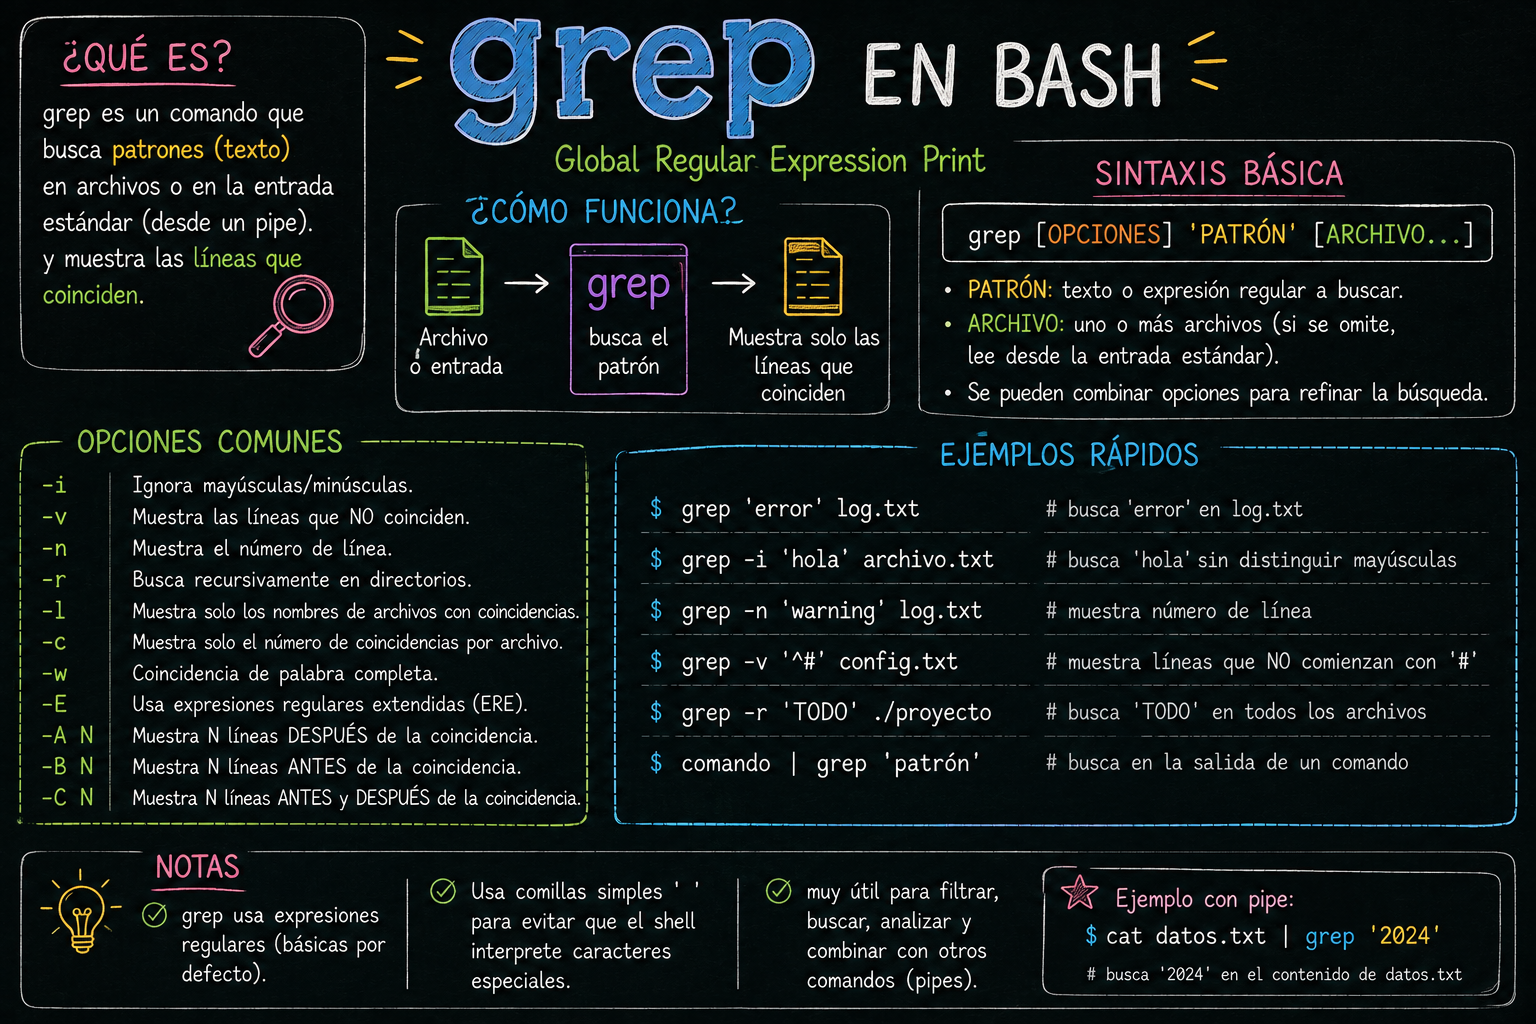
\includegraphics[keepaspectratio]{figures/bash_grep_overview.png}}

}

\caption{Imagen creada con ChatGPT.}

\end{figure}%

\section{\texorpdfstring{Opciones principales de
\texttt{grep}}{Opciones principales de grep}}\label{opciones-principales-de-grep}

Genera este primer archivo para los ejercicios:

\begin{Shaded}
\begin{Highlighting}[]
\BuiltInTok{echo} \AttributeTok{{-}e} \StringTok{"ab\textbackslash{}na+b\textbackslash{}nab\textbackslash{}naab\textbackslash{}nAnaplasma\textbackslash{}naaab\textbackslash{}nHola mundo\textbackslash{}nhola estudiantes\textbackslash{}nHOLA UNIVERSO"} \OperatorTok{\textgreater{}}\NormalTok{ archivo.txt}
\FunctionTok{cat}\NormalTok{ archivo.txt}
\end{Highlighting}
\end{Shaded}

\textbf{1. \texttt{-E} - Expresiones regulares extendidas}

Permite usar metacaracteres avanzados como \texttt{+}, \texttt{?},
\texttt{\textbar{}}, \texttt{\{\ \}}.

\begin{Shaded}
\begin{Highlighting}[]
\CommentTok{\# Sin {-}E: no funciona}
\FunctionTok{grep} \StringTok{"a+b"}\NormalTok{ archivo.txt      }\CommentTok{\# Busca "a+b" literal}

\CommentTok{\# Con {-}E: funciona}
\FunctionTok{grep} \AttributeTok{{-}E} \StringTok{"a+b"}\NormalTok{ archivo.txt   }\CommentTok{\# Busca "a", "ab", "aab", "aaab", etc.}
\end{Highlighting}
\end{Shaded}

\textbf{2. \texttt{-i} - Ignorar mayúsculas/minúsculas}

\begin{Shaded}
\begin{Highlighting}[]
\FunctionTok{grep} \AttributeTok{{-}i} \StringTok{"hola"}\NormalTok{ archivo.txt}
\CommentTok{\# Encuentra: "Hola", "HOLA", "hola", "HoLa"}
\end{Highlighting}
\end{Shaded}

Ahora genera este otro archivo:

\begin{Shaded}
\begin{Highlighting}[]
\BuiltInTok{echo} \AttributeTok{{-}e} \StringTok{"INFO: El sistema inició correctamente.\textbackslash{}nERROR: No se pudo abrir el archivo.\textbackslash{}nINFO: Conexión establecida.\textbackslash{}nWARNING: Memoria baja.\textbackslash{}nERROR: Fallo en la base de datos.\textbackslash{}nINFO: Proceso terminado."} \OperatorTok{\textgreater{}}\NormalTok{ archivo.log}
\FunctionTok{cat}\NormalTok{ archivo.log}
\end{Highlighting}
\end{Shaded}

\textbf{3. \texttt{-v} - Invertir búsqueda (líneas que NO coinciden)}

\begin{Shaded}
\begin{Highlighting}[]
\FunctionTok{grep} \AttributeTok{{-}v} \StringTok{"ERROR"}\NormalTok{ archivo.log}
\CommentTok{\# Imprime todas las líneas que NO contienen "ERROR"}
\end{Highlighting}
\end{Shaded}

\textbf{4. \texttt{-c} - Contar coincidencias}

\begin{Shaded}
\begin{Highlighting}[]
\FunctionTok{grep} \AttributeTok{{-}c} \StringTok{"ERROR"}\NormalTok{ archivo.log}
\CommentTok{\# Output: 2 (número de líneas con "ERROR")}
\end{Highlighting}
\end{Shaded}

\textbf{5. \texttt{-n} - Mostrar número de línea}

\begin{Shaded}
\begin{Highlighting}[]
\FunctionTok{grep} \AttributeTok{{-}n} \StringTok{"ERROR"}\NormalTok{ archivo.log}
\CommentTok{\# Output: }
\CommentTok{\# 2:ERROR: No se pudo abrir el archivo.}
\CommentTok{\# 5:ERROR: Fallo en la base de datos.}
\end{Highlighting}
\end{Shaded}

\textbf{6. \texttt{-l} - Mostrar solo nombres de archivos que contienen
la palabra}

\begin{Shaded}
\begin{Highlighting}[]
\FunctionTok{grep} \AttributeTok{{-}l} \StringTok{"ERROR"} \PreprocessorTok{*}\NormalTok{.log}
\CommentTok{\# Output: archivo.log}
\end{Highlighting}
\end{Shaded}

\textbf{7. \texttt{-r} - Buscar recursivamente en directorios}

\begin{Shaded}
\begin{Highlighting}[]
\FunctionTok{grep} \AttributeTok{{-}r} \StringTok{"ERROR"}\NormalTok{ /var/log/}
\CommentTok{\# Busca en todos los archivos del directorio /var/log/}
\end{Highlighting}
\end{Shaded}

\textbf{8. \texttt{-o} -} Mostrar solo la parte que coincide \textbf{+
\texttt{-i}} para ignorar las mayúsculas

\begin{Shaded}
\begin{Highlighting}[]
\FunctionTok{grep} \AttributeTok{{-}oi} \StringTok{"hola"}\NormalTok{ archivo.txt}
\CommentTok{\# Output: }
\CommentTok{\# Hola}
\CommentTok{\# hola}
\CommentTok{\#HOLA}
\end{Highlighting}
\end{Shaded}

\begin{figure}[H]

{\centering \pandocbounded{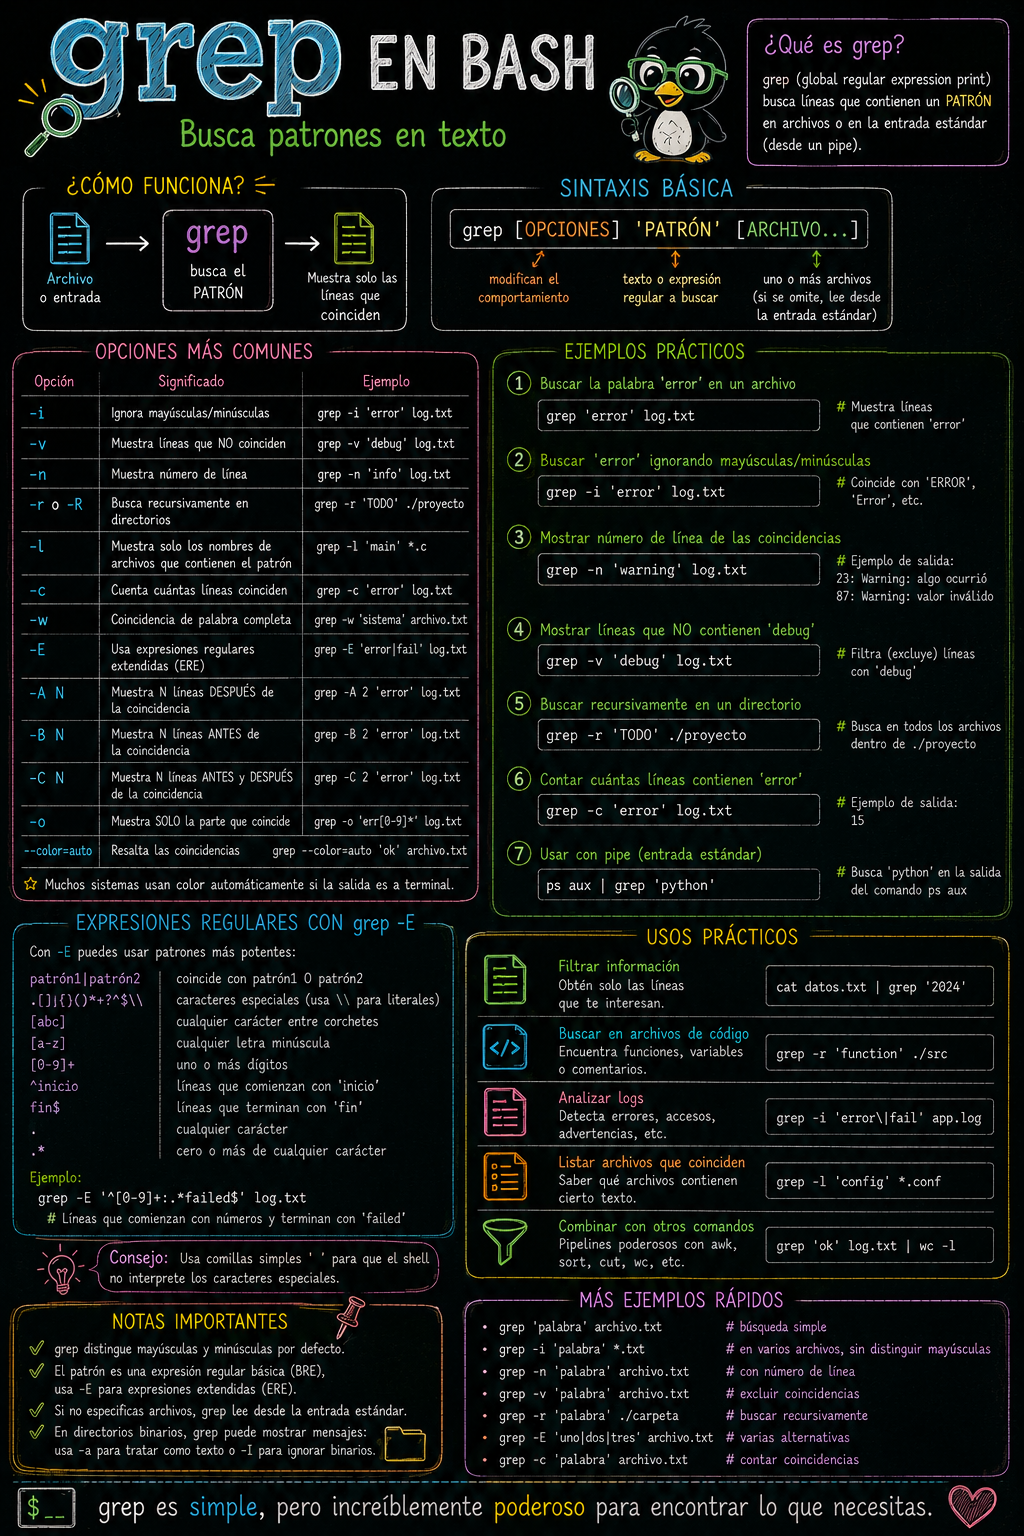
\includegraphics[keepaspectratio]{figures/bash_grep.png}}

}

\caption{Imagen creada con ChatGPT.}

\end{figure}%

\subsection{\texorpdfstring{Ejercicio 5 - \textbf{Dominar \texttt{grep}
(con
\texttt{echo\ -e})}}{Ejercicio 5 - Dominar grep (con echo -e)}}\label{ejercicio-5---dominar-grep-con-echo--e}

\begin{enumerate}
\def\labelenumi{\arabic{enumi}.}
\tightlist
\item
  Crea los archivos que usaremos y verificar su contenido en este
  ejercicio:
\end{enumerate}

\begin{Shaded}
\begin{Highlighting}[]
\CommentTok{\# Crear directorio de trabajo}
\FunctionTok{mkdir}\NormalTok{ ejercicio\_grep}
\BuiltInTok{cd}\NormalTok{ ejercicio\_grep}

\CommentTok{\# Crear archivo de usuarios}
\BuiltInTok{echo} \AttributeTok{{-}e} \StringTok{"juan@ejemplo.com 25 activo\textbackslash{}nmaria@empresa.es 30 inactivo\textbackslash{}ncarlos123 28 activo\textbackslash{}nana@dominio.org 22 activo\textbackslash{}npedro@test 35 inactivo\textbackslash{}nsofia@dominio.com 27 activo\textbackslash{}nluis@empresa.es 40 inactivo"} \OperatorTok{\textgreater{}}\NormalTok{ usuarios.txt}
\FunctionTok{cat}\NormalTok{ usuarios.txt}

\CommentTok{\# Crear archivo de log}
\BuiltInTok{echo} \AttributeTok{{-}e} \StringTok{"[2024{-}01{-}15 10:30:45] [INFO] Sistema iniciado\textbackslash{}n[2024{-}01{-}15 10:31:12] [ERROR] Conexión fallida a base de datos\textbackslash{}n[2024{-}01{-}15 10:32:00] [WARNING] Memoria disponible baja\textbackslash{}n[2024{-}01{-}15 10:33:45] [ERROR] Archivo no encontrado: config.ini\textbackslash{}n[2024{-}01{-}15 10:34:20] [INFO] Proceso de sincronización completado\textbackslash{}n[2024{-}01{-}15 10:35:10] [ERROR] Timeout en conexión remota\textbackslash{}n[2024{-}01{-}15 10:36:00] [WARNING] Espacio en disco bajo\textbackslash{}n[2024{-}01{-}15 10:37:30] [INFO] Backup completado exitosamente"} \OperatorTok{\textgreater{}}\NormalTok{ sistema.log}
\FunctionTok{cat}\NormalTok{ sistema.log}

\CommentTok{\# Crear archivo de productos}
\BuiltInTok{echo} \AttributeTok{{-}e} \StringTok{"001 Laptop Dell 1200.50 disponible\textbackslash{}n002 Mouse Logitech 25.99 disponible\textbackslash{}n003 Teclado Mecánico 89.99 agotado\textbackslash{}n004 Monitor LG 350.00 disponible\textbackslash{}n005 Webcam HD 45.50 disponible\textbackslash{}n006 Auriculares Sony 150.00 agotado\textbackslash{}n007 Cable HDMI 12.99 disponible\textbackslash{}n008 Hub USB 35.75 disponible"} \OperatorTok{\textgreater{}}\NormalTok{ productos.txt}
\FunctionTok{cat}\NormalTok{ productos.txt}

\CommentTok{\# Crear archivo de emails}
\BuiltInTok{echo} \AttributeTok{{-}e} \StringTok{"juan.perez@ejemplo.com\textbackslash{}nmaria\_lopez@empresa.es\textbackslash{}ncarlos.garcia@test.com\textbackslash{}nana.martinez@dominio.org\textbackslash{}npedro123@invalid\textbackslash{}nsofia.rodriguez@empresa.es\textbackslash{}nluis\_fernandez@test.org\textbackslash{}ncontacto@empresa.es"} \OperatorTok{\textgreater{}}\NormalTok{ emails.txt}
\FunctionTok{cat}\NormalTok{ emails.txt}

\CommentTok{\# Crear archivo de géneros bacterianos}
\BuiltInTok{echo} \AttributeTok{{-}e} \StringTok{"Rickettsia\textbackslash{}nOrientia\textbackslash{}nWolbachia\textbackslash{}nAegyptianella\textbackslash{}nAnaplasma\textbackslash{}nCowdria\textbackslash{}nEhrlichia\textbackslash{}nNeorickettsia\textbackslash{}nCaedibacter\textbackslash{}nHolospora\textbackslash{}nLyticum\textbackslash{}nOdyssella\textbackslash{}nSymbiotes\textbackslash{}nTectibacter"} \OperatorTok{\textgreater{}}\NormalTok{ bacterias\_generos.txt}
\FunctionTok{cat}\NormalTok{ bacterias\_generos.txt}
\end{Highlighting}
\end{Shaded}

\begin{enumerate}
\def\labelenumi{\arabic{enumi}.}
\setcounter{enumi}{1}
\item
  Buscar los usuarios activos dentro del archivo \texttt{usuarios.txt}.
  NOTA: \texttt{\textbackslash{}b} no representa un carácter real, sino
  una \textbf{posición} en el texto donde termina o comienza una
  palabra.
\item
  Buscar los errores en el archivo log \texttt{sistema.log}.
\item
  Buscar productos disponibles en el archivo \texttt{productos.txt}.
\item
  Ignorar las mayúsculas/minúsculas (\texttt{-i}) de
  \texttt{sistema.log}.
\item
  Contar el número (\texttt{grep\ -c}) de usuarios activos en el archivo
  \texttt{usuarios.txt}.
\item
  Dime en que líneas (\texttt{grep\ -n}) aparece la palabra ERROR en
  \texttt{sistema.log}.
\item
  Mostrar solo las coincidencias (\texttt{grep\ -o}) con la palabra
  ERROR en \texttt{sistema.log}.
\item
  Buscar las especies que comienzan con A en el archivo
  \texttt{bacterias\_generos.txt}.
\item
  Buscar las especies que comienzan con R o W en el archivo
  \texttt{bacterias\_generos.txt}.

  \begin{tcolorbox}[enhanced jigsaw, arc=.35mm, bottomrule=.15mm, bottomtitle=1mm, breakable, colback=white, colbacktitle=quarto-callout-tip-color!10!white, colframe=quarto-callout-tip-color-frame, coltitle=black, left=2mm, leftrule=.75mm, opacityback=0, opacitybacktitle=0.6, rightrule=.15mm, title={Solución}, titlerule=0mm, toprule=.15mm, toptitle=1mm]

\begin{Shaded}
\begin{Highlighting}[]
\ExtensionTok{2.}\NormalTok{ grep }\AttributeTok{{-}E} \StringTok{"\textbackslash{}bactivo\textbackslash{}b"}\NormalTok{ usuarios.txt o grep }\StringTok{" activo"}\NormalTok{ usuarios.txt}
\ExtensionTok{3.}\NormalTok{ grep }\StringTok{"ERROR"}\NormalTok{ sistema.log}
\ExtensionTok{4.}\NormalTok{ grep }\StringTok{"disponible"}\NormalTok{ productos.txt}
\ExtensionTok{5.}\NormalTok{ grep }\AttributeTok{{-}i} \StringTok{"error"}\NormalTok{ sistema.log}
\ExtensionTok{6.}\NormalTok{ grep }\StringTok{" activo"}\NormalTok{ usuarios.txt }\KeywordTok{|} \FunctionTok{wc} \AttributeTok{{-}l}\NormalTok{ o grep }\AttributeTok{{-}c} \StringTok{" activo"}\NormalTok{ usuarios.txt }
\ExtensionTok{7.}\NormalTok{ grep }\AttributeTok{{-}n} \StringTok{"ERROR"}\NormalTok{ sistema.log}
\ExtensionTok{8.}\NormalTok{ grep }\AttributeTok{{-}o} \StringTok{"ERROR"}\NormalTok{ sistema.log}
\ExtensionTok{9.}\NormalTok{ grep }\StringTok{"\^{}A"}\NormalTok{ bacterias\_generos.txt}
\ExtensionTok{10.}\NormalTok{ grep }\AttributeTok{{-}E} \StringTok{"\^{}(R|W)"}\NormalTok{ bacterias\_generos.txt}
\end{Highlighting}
\end{Shaded}

  \end{tcolorbox}
\end{enumerate}

\section{Ejercicios de repaso}\label{ejercicios-de-repaso}

Puedes seguir repasando y aprendiendo de las expresiones regulares en la
pagina de \href{https://regexone.com/}{RegexOne}.

\textbf{Rangos comunes}:

\begin{itemize}
\tightlist
\item
  \texttt{{[}a-z{]}} = letras minúsculas
\item
  \texttt{{[}A-Z{]}} = letras mayúsculas
\item
  \texttt{{[}0-9{]}} = dígitos
\item
  \texttt{{[}a-zA-Z{]}} = letras (mayúsculas y minúsculas)
\item
  \texttt{{[}a-zA-Z0-9{]}} = letras y dígitos
\end{itemize}

\begin{tcolorbox}[enhanced jigsaw, arc=.35mm, bottomrule=.15mm, bottomtitle=1mm, breakable, colback=white, colbacktitle=quarto-callout-warning-color!10!white, colframe=quarto-callout-warning-color-frame, coltitle=black, left=2mm, leftrule=.75mm, opacityback=0, opacitybacktitle=0.6, rightrule=.15mm, title=\textcolor{quarto-callout-warning-color}{\faExclamationTriangle}\hspace{0.5em}{Advertencia}, titlerule=0mm, toprule=.15mm, toptitle=1mm]

El operador \texttt{\textgreater{}} sobre escribe archivos. Ten cuidado
al usarlo para que no pierdas datos.

\end{tcolorbox}

\section{Material suplementario}\label{material-suplementario-4}

\begin{itemize}
\tightlist
\item
  RSG Ecuador.
  \href{https://rsg-ecuador.github.io/unix.bioinfo.rsgecuador/content/Curso_avanzado/02_Bash/1_bash.html}{Scripts
  en Bash}
\item
  RSG Ecuador.
  \href{https://rsg-ecuador.github.io/unix.bioinfo.rsgecuador/content/Curso_basico/03_Manejo_terminal/5_wildcards.html}{Wildcards
  y Streams}
\item
  RSG Ecuador.
  \href{https://rsg-ecuador.github.io/unix.bioinfo.rsgecuador/content/Curso_basico/04_Procesamiento_ficheros_regex_pipes/3_Expresiones_regulares.html}{Expresiones
  regulares (\emph{regex})}
\item
  \href{https://pressbooks.senecapolytechnic.ca/uli101/chapter/wildcard-selection-in-bash/}{Wildcard
  Selection in Bash}
\item
  \href{https://twiki.org/cgi-bin/view/Codev/TWikiPresentation2017x06x01Regex}{Expresiones
  regulares}
\end{itemize}

\part{\textbf{Sección 4} - Edición de archivos con Bash}

\chapter{\texorpdfstring{Edición de archivos con los editores de texto
(\texttt{nano} y
\texttt{vim})}{Edición de archivos con los editores de texto (nano y vim)}}\label{ediciuxf3n-de-archivos-con-los-editores-de-texto-nano-y-vim}

\begin{quote}
\textbf{Fecha:} 22 de septiembre, 2026
\end{quote}

Los editores de texto nos permiten hacer desde ligeros hasta cambios u
operaciones masivas en el contenido de nuestros archivos. Existen varias
herramientas para esto pero las más populares son ``nano'' y ``vim''.

\begin{figure}[H]

{\centering \pandocbounded{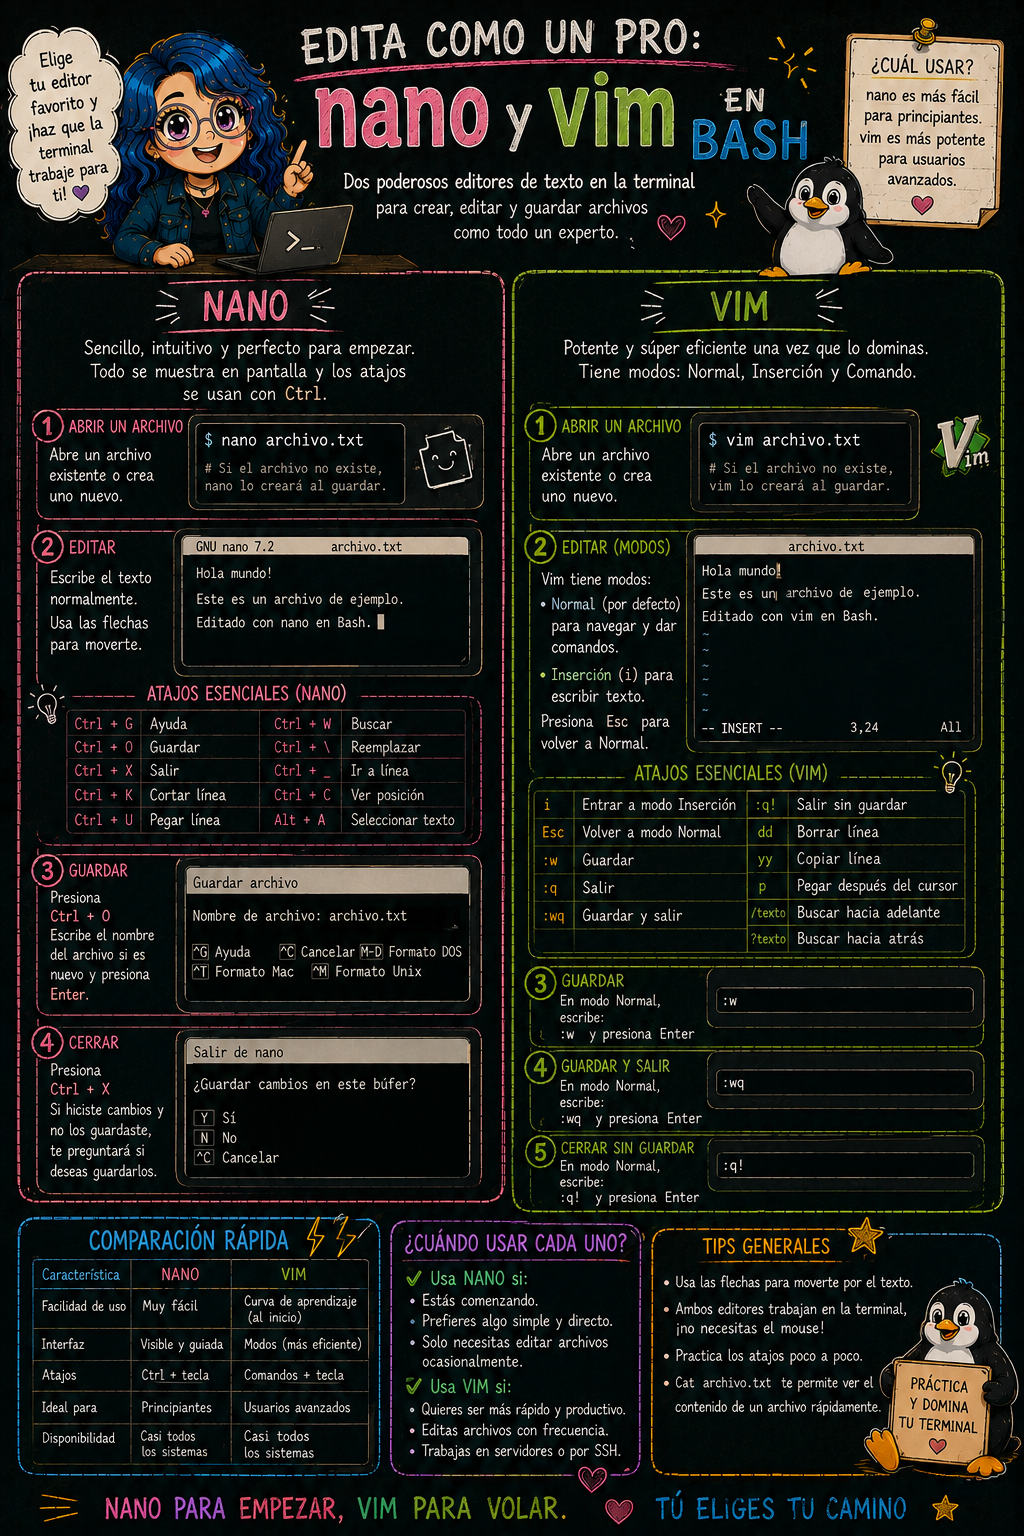
\includegraphics[keepaspectratio]{figures/bash_nano_y_vim.png}}

}

\caption{Imagen creada con ChatGPT.}

\end{figure}%

\subsection{Nano}\label{nano}

Para utilizar nano, debemos de seguir una serie de comandos. Primero
creamos/leemos nuestro archivo.

\begin{Shaded}
\begin{Highlighting}[]
\FunctionTok{nano}\NormalTok{ mi{-}archivo{-}nano.txt}
\end{Highlighting}
\end{Shaded}

Esto nos creará un archivo de texto al que podemos ingresar información
y además nos va desplegar un menú de opciones en la parte inferior de
nuestra terminal.

\begin{center}
\pandocbounded{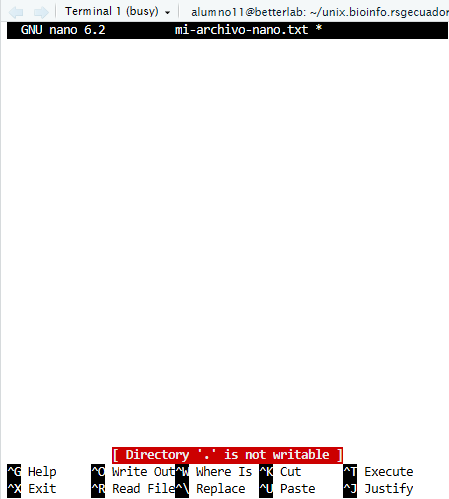
\includegraphics[keepaspectratio]{figures/terminal_example.png}}
\end{center}

Para utilizar estas opciones se usan shorchuts o atajos en el teclado,
en las que el símbolo~\texttt{\^{}}~significa la
tecla~\texttt{Control}~o~\texttt{Command}~y la~\texttt{M}~es la
tecla~\texttt{Alt}. En nuestro caso donde queremos agregar texto,
simplemente escribimos:

\begin{tcolorbox}[enhanced jigsaw, arc=.35mm, bottomrule=.15mm, bottomtitle=1mm, breakable, colback=white, colbacktitle=quarto-callout-note-color!10!white, colframe=quarto-callout-note-color-frame, coltitle=black, left=2mm, leftrule=.75mm, opacityback=0, opacitybacktitle=0.6, rightrule=.15mm, title={Ejercicio 6. Edición de archivos con nano}, titlerule=0mm, toprule=.15mm, toptitle=1mm]

\begin{enumerate}
\def\labelenumi{\arabic{enumi}.}
\tightlist
\item
  Crea un archivo nano con el nombre ``mi-archivo-nano.txt''.
  \texttt{nano\ mi-archivo-nano.txt}
\item
  Agrega la siguiente información a tu archivo.
  \texttt{Hola\ mi\ nombre\ es\ NOMBRE\ y\ este\ es\ mi\ primer\ archivo\ nano.}
\item
  Utiliza \texttt{ctrl\ +\ x} para salir y guardar la información,
  presiona \texttt{Enter} para cerrar el editor.
\end{enumerate}

\end{tcolorbox}

Para guardar los cambios en el archivo presionamos
\texttt{control\ +\ x}, el programa nos desplegará un mensaje para
guardar el archivo. Presionamos \textbf{enter} y ahora podemos verificar
el contenido.

\begin{Shaded}
\begin{Highlighting}[]
\FunctionTok{cat}\NormalTok{ mi{-}archivo{-}nano.txt}
\end{Highlighting}
\end{Shaded}

\subsection{Vim}\label{vim}

Vim tiene ligeros cambios en su modo de uso:

\begin{Shaded}
\begin{Highlighting}[]
\ExtensionTok{vim}\NormalTok{ mi{-}archivo{-}vim.txt }
\end{Highlighting}
\end{Shaded}

A diferencia de \texttt{nano}, no podemos ingresar texto directamente en
el archivo y hay algo que se conoce como modos. En este primer modo
normal puedes accesar a distintas otras funcionalidades, para cambiar a
modo escritura o modo inserción de texto, debemos presionar \texttt{i}.

Una vez dentro del modo inserción, escribimos el siguiente texto:

\begin{tcolorbox}[enhanced jigsaw, arc=.35mm, bottomrule=.15mm, bottomtitle=1mm, breakable, colback=white, colbacktitle=quarto-callout-note-color!10!white, colframe=quarto-callout-note-color-frame, coltitle=black, left=2mm, leftrule=.75mm, opacityback=0, opacitybacktitle=0.6, rightrule=.15mm, title={Ejercicio 7. Edición de archivos con vim}, titlerule=0mm, toprule=.15mm, toptitle=1mm]

\begin{enumerate}
\def\labelenumi{\arabic{enumi}.}
\tightlist
\item
  Crea un archivo nano con el nombre ``mi-archivo-vim.txt''.
  \texttt{vim\ mi-archivo-vim.txt}
\item
  Agrega la siguiente información a tu archivo.
  \texttt{Hola\ mi\ nombre\ es\ NOMBRE\ y\ este\ es\ mi\ primer\ archivo\ vim.}
\item
  Utiliza \texttt{ctrl\ +\ x} para salir y guardar la información,
  presiona \texttt{Enter} para cerrar el editor.
\end{enumerate}

\end{tcolorbox}

para guardar los cambios debemos presionar la tecla \texttt{Esc}, para
salir del modo inserción y teclear:

\begin{Shaded}
\begin{Highlighting}[]
\ExtensionTok{:wq}
\end{Highlighting}
\end{Shaded}

En donde:

\begin{tcolorbox}[enhanced jigsaw, arc=.35mm, bottomrule=.15mm, bottomtitle=1mm, breakable, colback=white, colbacktitle=quarto-callout-note-color!10!white, colframe=quarto-callout-note-color-frame, coltitle=black, left=2mm, leftrule=.75mm, opacityback=0, opacitybacktitle=0.6, rightrule=.15mm, title={Explicación}, titlerule=0mm, toprule=.15mm, toptitle=1mm]

\begin{itemize}
\tightlist
\item
  \texttt{w} = write, indica a la terminal guardar los cambios
\item
  \texttt{q} = quit, indica salir de la edición del archivo.
\end{itemize}

\end{tcolorbox}

Para ambos editores puedes accesar al manual del usuario proporcionados
dentro de la terminal usando cualquiera de los siguientes comandos:

\begin{itemize}
\tightlist
\item
  Para ver el manual completo de \texttt{vim} escribe:
\end{itemize}

\begin{Shaded}
\begin{Highlighting}[]
\FunctionTok{man}\NormalTok{ vim}
\end{Highlighting}
\end{Shaded}

\begin{itemize}
\tightlist
\item
  Para ver el manual completo de \texttt{nano} escribe:
\end{itemize}

\begin{Shaded}
\begin{Highlighting}[]
\FunctionTok{man}\NormalTok{ nano}
\end{Highlighting}
\end{Shaded}

\section{Referencias}\label{referencias-5}

\begin{itemize}
\tightlist
\item
  \href{https://victorhck.gitbook.io/aprende-vim}{Aprende vim}
\end{itemize}

\chapter{Crear un R Project}\label{crear-un-r-project}

\begin{quote}
\textbf{Fecha:} 22 de septiembre, 2026
\end{quote}

Al comenzar a trabajar con R y RStudio, ya sea para crear un programa
para un proyecto, crear una aplicación, presentación, blog, paquete,
etc, es recomendado crear un \textbf{R project}.

\section{¿Qué es un R Project y por qué
usarlo?}\label{quuxe9-es-un-r-project-y-por-quuxe9-usarlo}

\begin{itemize}
\item
  \textbf{Carpeta de trabajo dedicada}: al crear un R Project, RStudio
  genera automáticamente una carpeta que contiene todos los archivos y
  configuraciones necesarias para tu proyecto.
\item
  \textbf{Organización}: te permite mantener en un solo lugar tus
  scripts, datos, variables y documentos relacionados.
\item
  \textbf{Reproducibilidad}: facilita que cualquier persona (incluido tú
  en el futuro) pueda abrir el proyecto y trabajar con el mismo entorno.
\item
  \textbf{Integración con Git/GitHub}: al tener el mismo nombre que tu
  repositorio, se asegura una sincronización más clara y ordenada entre
  tu proyecto local y el repositorio remoto.
\end{itemize}

\section{\texorpdfstring{\textbf{¿Cómo iniciamos un R
project?}}{¿Cómo iniciamos un R project?}}\label{cuxf3mo-iniciamos-un-r-project}

\begin{enumerate}
\def\labelenumi{\arabic{enumi}.}
\tightlist
\item
  Vayamos en la parte superior al menú \textbf{Archivos \textgreater{}
  Nuevo Proyecto}.
\end{enumerate}

\pandocbounded{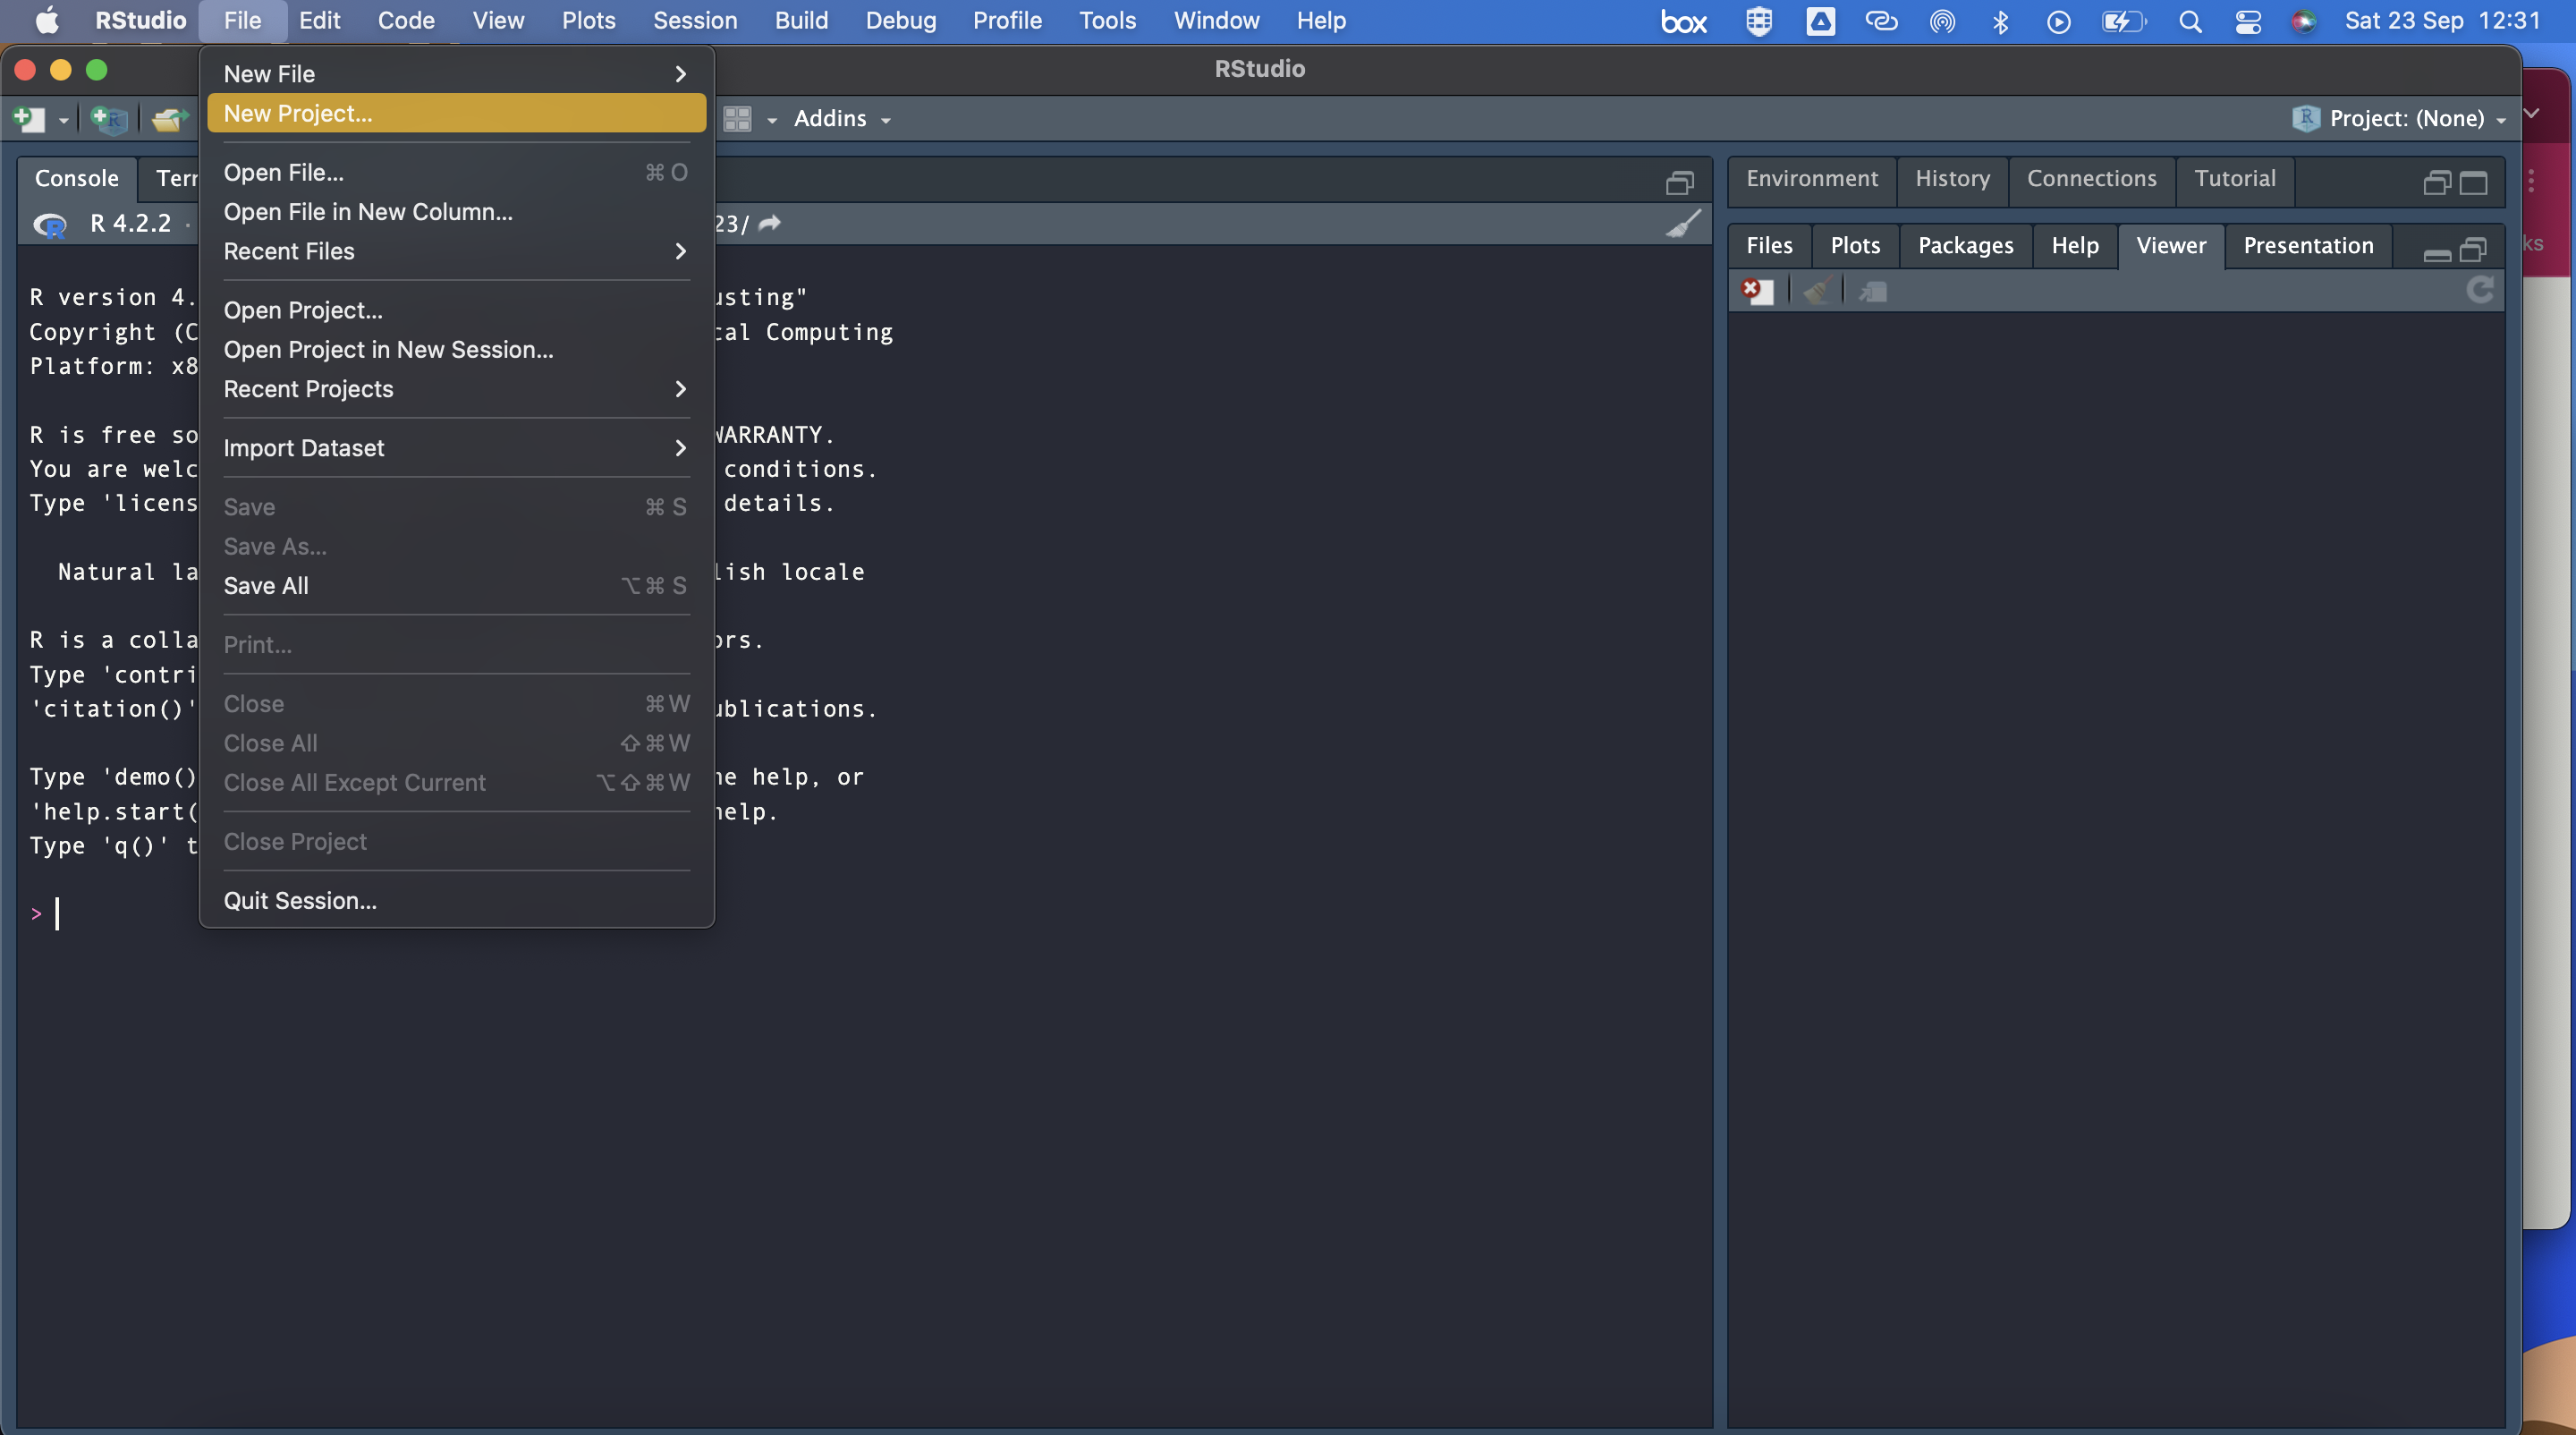
\includegraphics[keepaspectratio]{figures/rproject_paso1.png}}

\begin{enumerate}
\def\labelenumi{\arabic{enumi}.}
\setcounter{enumi}{1}
\tightlist
\item
  Seleccionamos la opción de \textbf{Nuevo directorio}.
\end{enumerate}

\pandocbounded{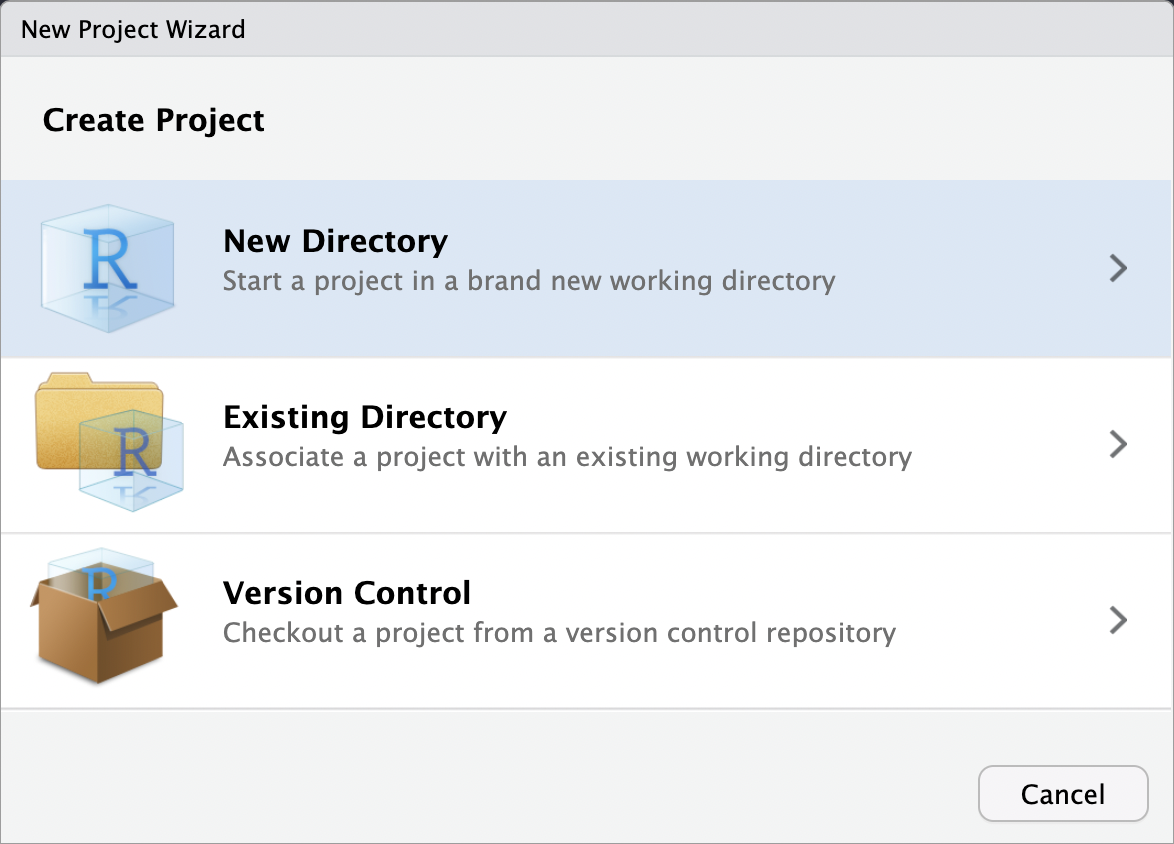
\includegraphics[keepaspectratio]{figures/rproject_paso2.png}}

\begin{enumerate}
\def\labelenumi{\arabic{enumi}.}
\setcounter{enumi}{2}
\tightlist
\item
  Seleccionamos el tipo de projecto que vamos a iniciar, en nuestro caso
  \textbf{Nuevo proyecto}.
\end{enumerate}

\pandocbounded{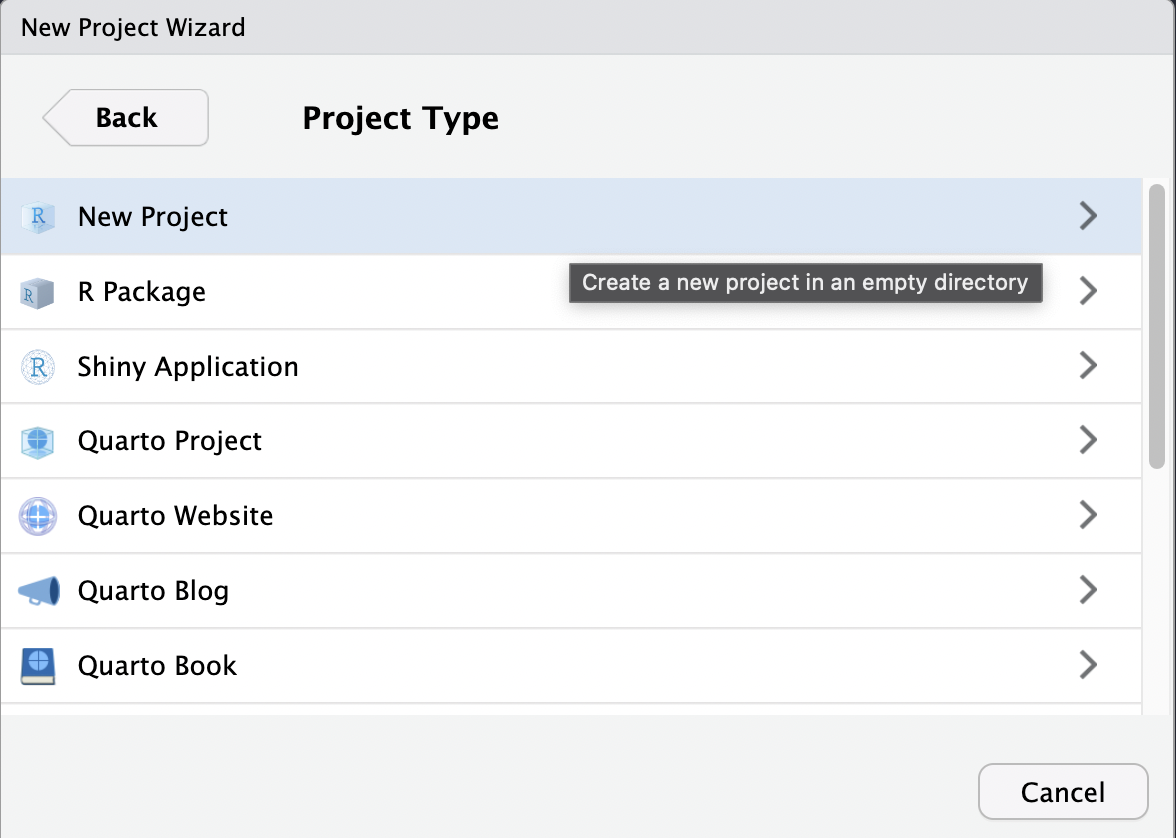
\includegraphics[keepaspectratio]{figures/rproject_paso3.png}}

\begin{enumerate}
\def\labelenumi{\arabic{enumi}.}
\setcounter{enumi}{3}
\tightlist
\item
  Nombramos el folder que crearemos y seleccionamos en dónde queremos
  que se almacene.
\end{enumerate}

\pandocbounded{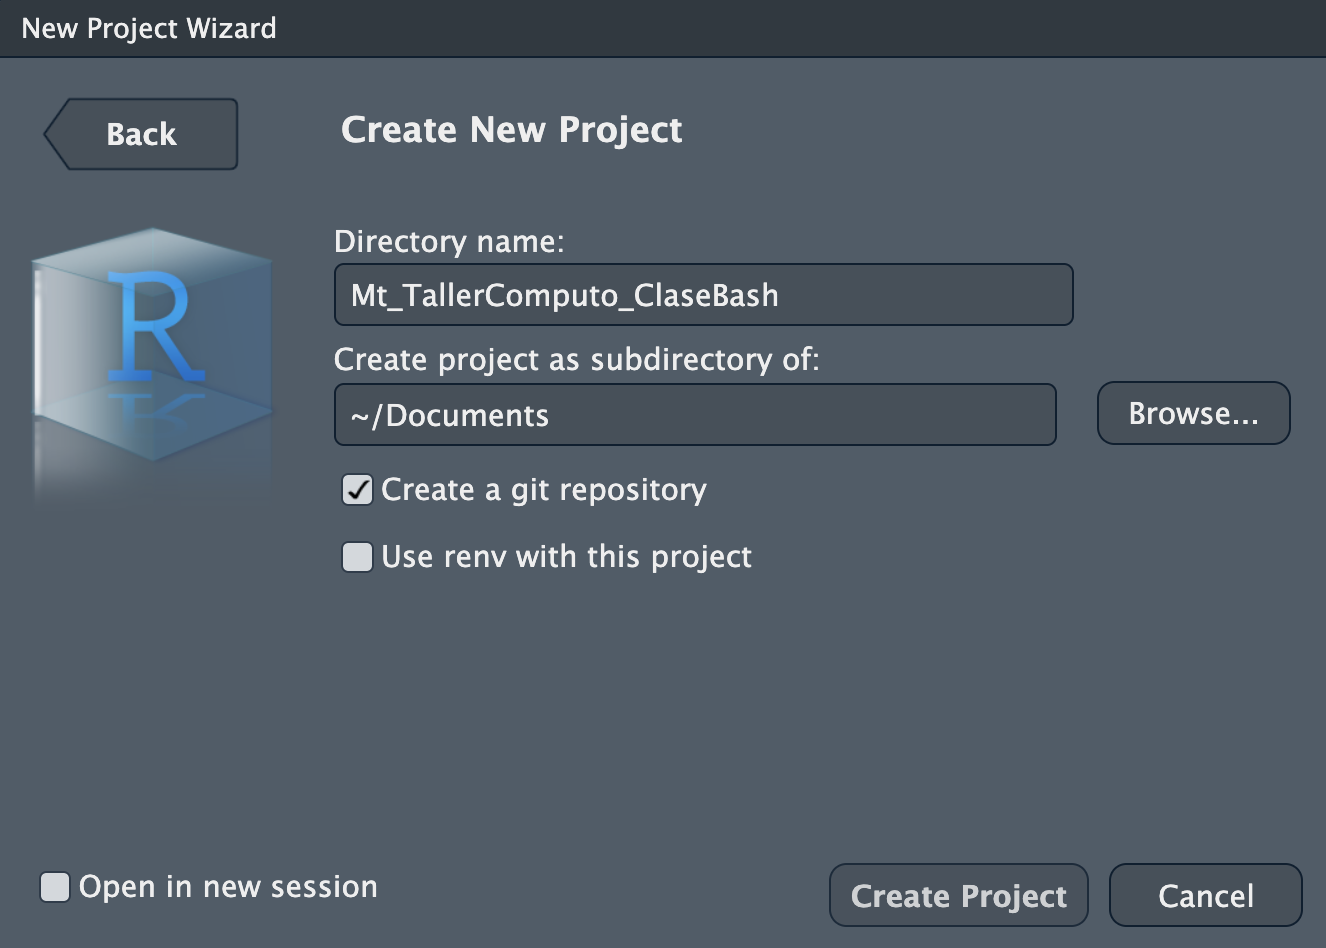
\includegraphics[keepaspectratio]{figures/rproject_paso4.png}}

\textbf{¡Felicidades, acabas de crear un R project!} Si vamos al folder
en donde creamos nuestro proyecto, podemos observar que se creó un
archivo con terminación \textbf{Rproj}, este es un archivo que contiene
la configuración específica para nuestro proyecto.

\begin{figure}[H]

{\centering 
\includegraphics[width=4.96875in,height=\textheight,keepaspectratio]{figures/rproject.png}

}

\caption{Imagen tomada de: Allison Horst}

\end{figure}%

\subsection{Directorio de trabajo}\label{directorio-de-trabajo}

Este archivo (\textbf{Rproj}) también establece como \textbf{directorio
de trabajo} el folder en donde iniciamos el proyecto (puedes comprobarlo
desde la consola de RStudio, escribiendo el comando \texttt{getwd()}).
Esto es muy conveniente puesto que así podemos asegurarnos de que vamos
a acceder a los archivos que estén exclusivamente en nuestro entorno de
trabajo.

Coloca en la consola dentro de Rstudio:

\begin{Shaded}
\begin{Highlighting}[]
\FunctionTok{getwd}\NormalTok{()}
\end{Highlighting}
\end{Shaded}

\begin{verbatim}
[1] "/Users/ecoss/Documents/Mt2026_Taller_Computo_libro"
\end{verbatim}

\section{Crear un Rscript}\label{crear-un-rscript}

Para comenzar a trabajar en un proyecto, necesitamos crear un archivo
para escribir nuestro programa. Entra en \textbf{Archivo \textgreater{}
Nuevo Archivo}.

Podemos ver que tenemos distintas opciones de archivos que podemos
crear, en este caso vamos a crear nuestro primer \textbf{Rscript}.

\pandocbounded{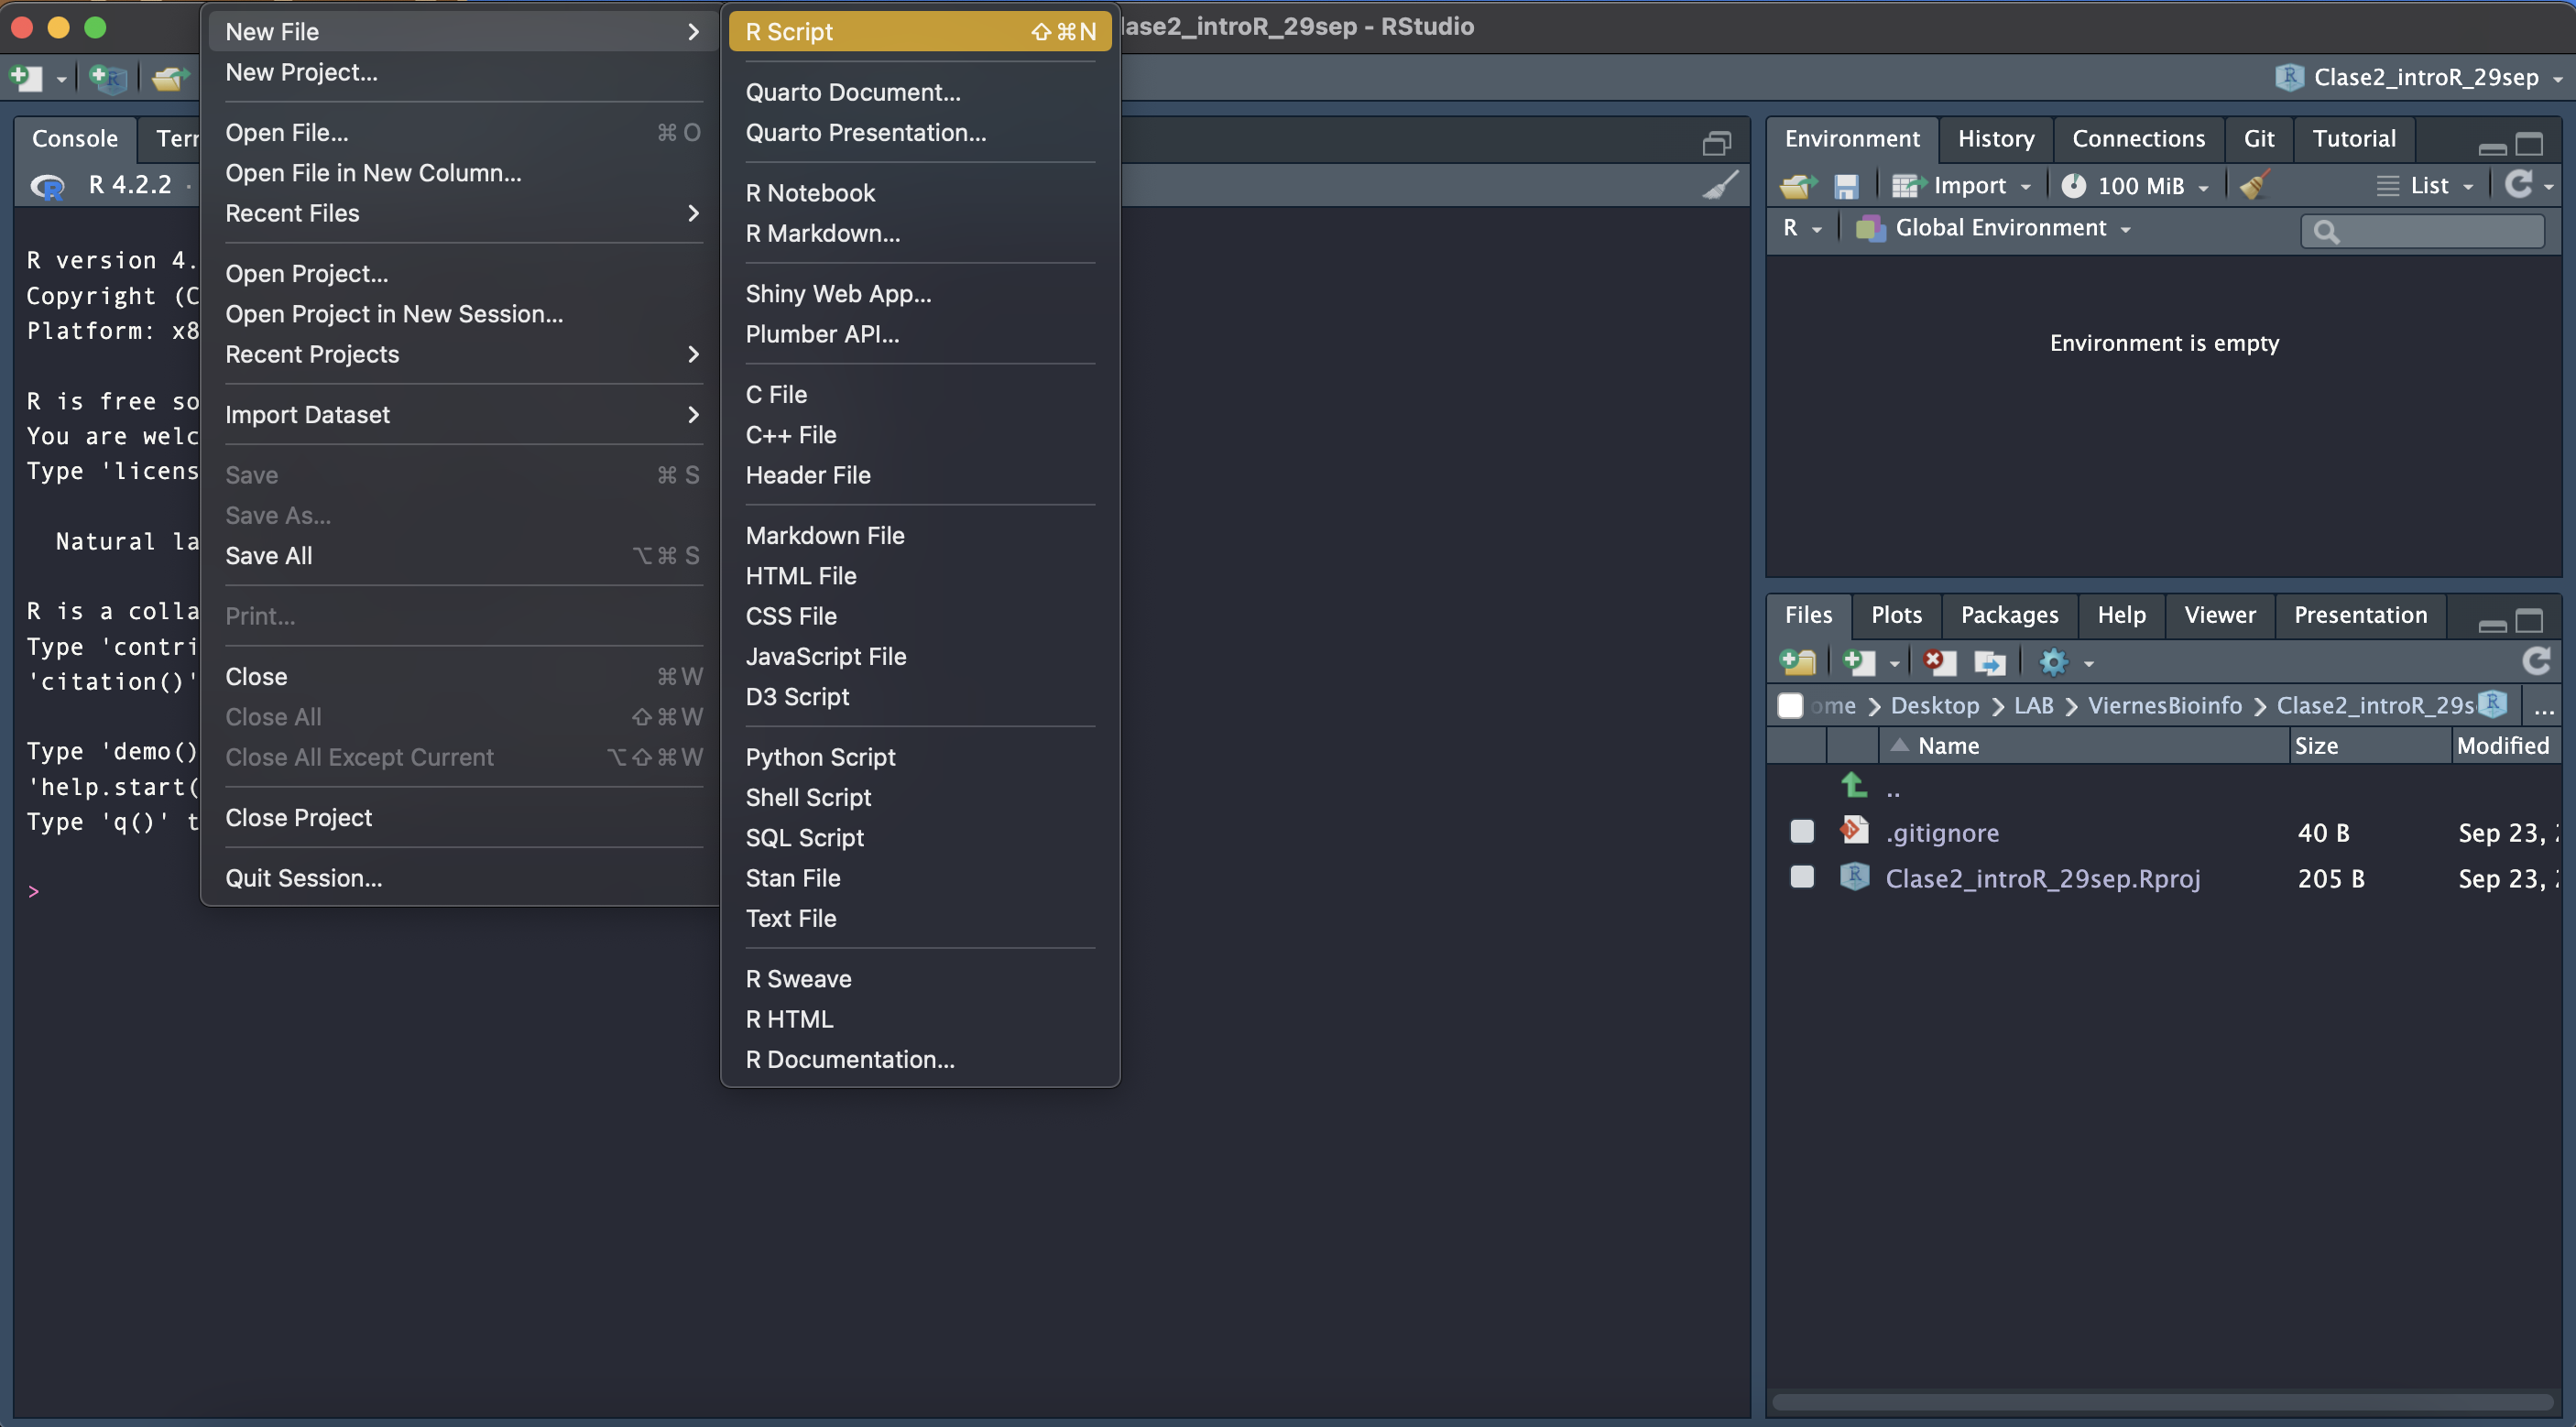
\includegraphics[keepaspectratio]{figures/rscript_paso1.png}}

\subsection{\texorpdfstring{\textbf{¿Qué es un
Rscript?}}{¿Qué es un Rscript?}}\label{quuxe9-es-un-rscript}

Es simplemente un archivo de texto con las instrucciones de nuestro
algoritmo escritas en el lenguaje de R. También contiene nuestros
comentarios escritos con \texttt{\#}.

Intenta escribir tu primer Rscript en el \textbf{editor}, copiando el
siguiente algoritmo para realizar una suma:

\begin{Shaded}
\begin{Highlighting}[]
\NormalTok{a }\OtherTok{\textless{}{-}} \DecValTok{2}
\NormalTok{b }\OtherTok{\textless{}{-}} \DecValTok{3}
\NormalTok{suma }\OtherTok{=}\NormalTok{ a }\SpecialCharTok{+}\NormalTok{ b}
\NormalTok{suma}
\end{Highlighting}
\end{Shaded}

\begin{verbatim}
[1] 5
\end{verbatim}

\section{\texorpdfstring{\textbf{¿Cómo ejecutamos el
código?}}{¿Cómo ejecutamos el código?}}\label{cuxf3mo-ejecutamos-el-cuxf3digo}

Selecciona todo el código, después ve a la parte superior de la ventana
del \textbf{editor} y da click en el botón \textbf{Run}. También pueden
ejecutar tu código línea por línea, poniendo tu cursor al principio o al
final de la linea y presionando las teclas \textbf{Control + Enter} o
\textbf{Command + Enter}.

\begin{figure}[H]

{\centering \pandocbounded{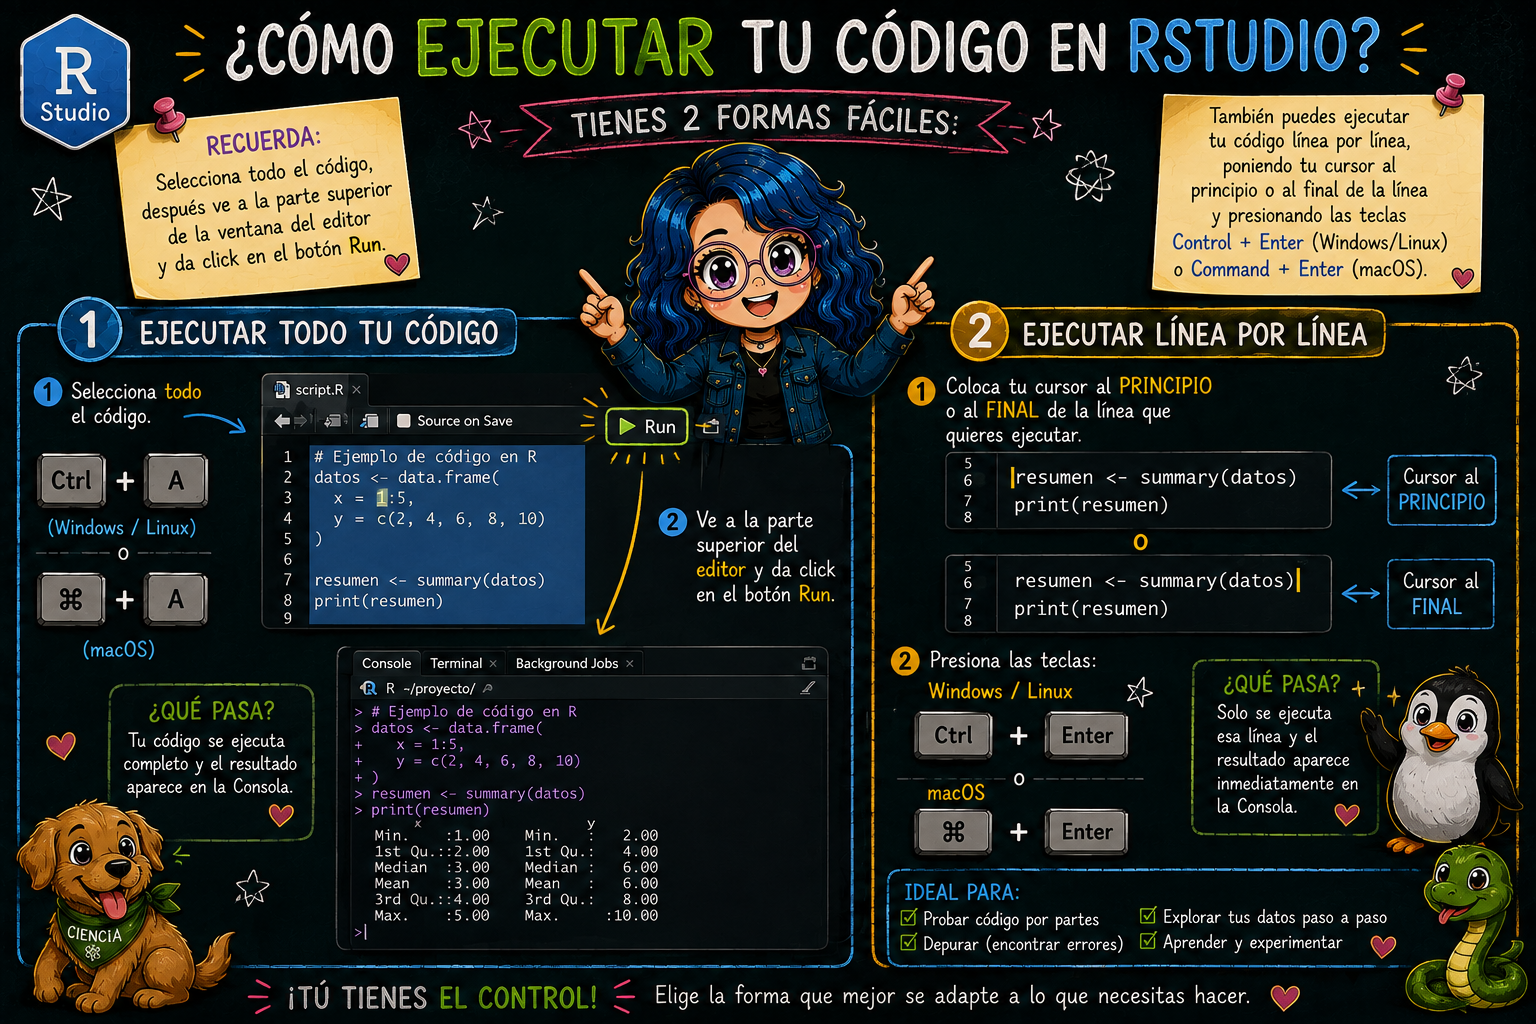
\includegraphics[keepaspectratio]{figures/rscript_run.png}}

}

\caption{Imagen creada con ChatGPT.}

\end{figure}%

\section{Hay más que solo Rscripts}\label{hay-muxe1s-que-solo-rscripts}

\begin{figure}[H]

{\centering \pandocbounded{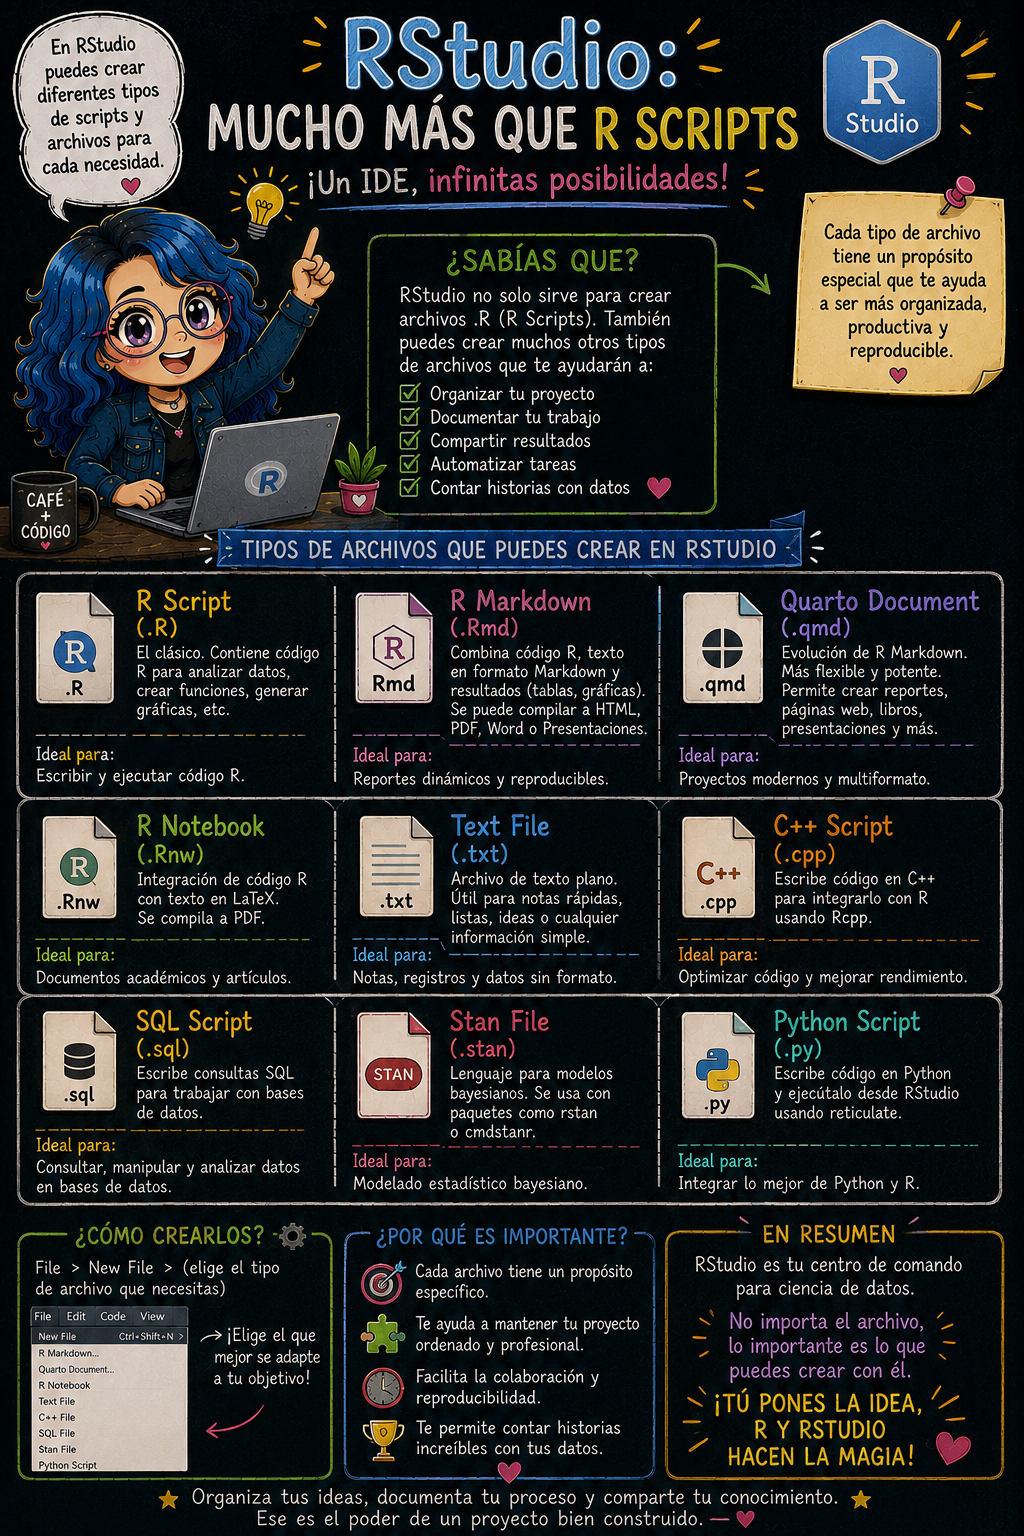
\includegraphics[keepaspectratio]{figures/rscript_overview.png}}

}

\caption{Imagen creada con ChatGPT.}

\end{figure}%

\chapter{\texorpdfstring{Edición de archivos con el editor de flujo
\texttt{sed}}{Edición de archivos con el editor de flujo sed}}\label{ediciuxf3n-de-archivos-con-el-editor-de-flujo-sed}

\begin{quote}
\textbf{Fecha:} 24 de septiembre, 2026
\end{quote}

\texttt{sed} (stream editor) es un \textbf{editor de flujo}, una potente
herramienta de tratamiento de texto para el sistema operativo UNIX que
acepta como entrada un archivo, lo lee y modifica línea a línea de
acuerdo a un script. \texttt{sed} permite manipular flujos de datos,
como por ejemplo cortar líneas, buscar y reemplazar texto (con soporte
de \textbf{expresiones regulares}), entre otras cosas.

Algunas de las operaciones más primordiales de sed son el cambio de
saltos de líneas, la sustitución de espacios por comas o tabulaciones,
la deleción o adición de strings, etc.

La sintaxis general de la orden \texttt{sed} es:

\begin{Shaded}
\begin{Highlighting}[]
\FunctionTok{sed} \PreprocessorTok{[{-}}\SpecialStringTok{n}\PreprocessorTok{]} \PreprocessorTok{[{-}}\SpecialStringTok{e}\StringTok{\textquotesingle{}script\textquotesingle{}}\PreprocessorTok{]}\NormalTok{ [{-}f archivo] archivo1 archivo2 ...}
\end{Highlighting}
\end{Shaded}

donde:

\begin{tcolorbox}[enhanced jigsaw, arc=.35mm, bottomrule=.15mm, bottomtitle=1mm, breakable, colback=white, colbacktitle=quarto-callout-note-color!10!white, colframe=quarto-callout-note-color-frame, coltitle=black, left=2mm, leftrule=.75mm, opacityback=0, opacitybacktitle=0.6, rightrule=.15mm, title={Explicación}, titlerule=0mm, toprule=.15mm, toptitle=1mm]

\begin{itemize}
\tightlist
\item
  \texttt{-n} indica que se suprima la salida estándar.
\item
  \texttt{-e} indica que se ejecute el script que viene a continuación.
\item
  \texttt{-f} indica que las órdenes se tomarán de un archivo.
\end{itemize}

\end{tcolorbox}

\subsubsection{\texorpdfstring{Ejemplo de sustitución con
\texttt{sed}}{Ejemplo de sustitución con sed}}\label{ejemplo-de-sustituciuxf3n-con-sed}

Sustituciones \texttt{s///} de palabras: \texttt{s/esto/aquello/}

\begin{Shaded}
\begin{Highlighting}[]
\BuiltInTok{echo} \StringTok{"Windows es lo máximo"} \KeywordTok{|} \FunctionTok{sed} \StringTok{\textquotesingle{}s/Windows/Linux/\textquotesingle{}}
\end{Highlighting}
\end{Shaded}

En el ejemplo anterior, la modificación se hace solamente en la primer
instancia que el comando encuentra. Pero esto no nos funciona si tenemos
400 repeticiones de Windows que queremos cambiar a Linux. Para que
funcione debemos hacer un cambio de la siquiente manera:

\begin{Shaded}
\begin{Highlighting}[]
\BuiltInTok{echo} \StringTok{"Windows es un sistema operativo ampliamente utilizado."} \OperatorTok{\textgreater{}}\NormalTok{ archivo.txt}
\FunctionTok{cat}\NormalTok{ archivo.txt}
\FunctionTok{sed} \StringTok{\textquotesingle{}s/Windows/Linux/g\textquotesingle{}}\NormalTok{ archivo.txt}
\end{Highlighting}
\end{Shaded}

Esta letra \textbf{g} que agregamos, indica hacer las sustituciones de
manera \textbf{global}, es decir en todas las ocurrencias o repeticiones
dentro de un archivo.

\begin{figure}[H]

{\centering \pandocbounded{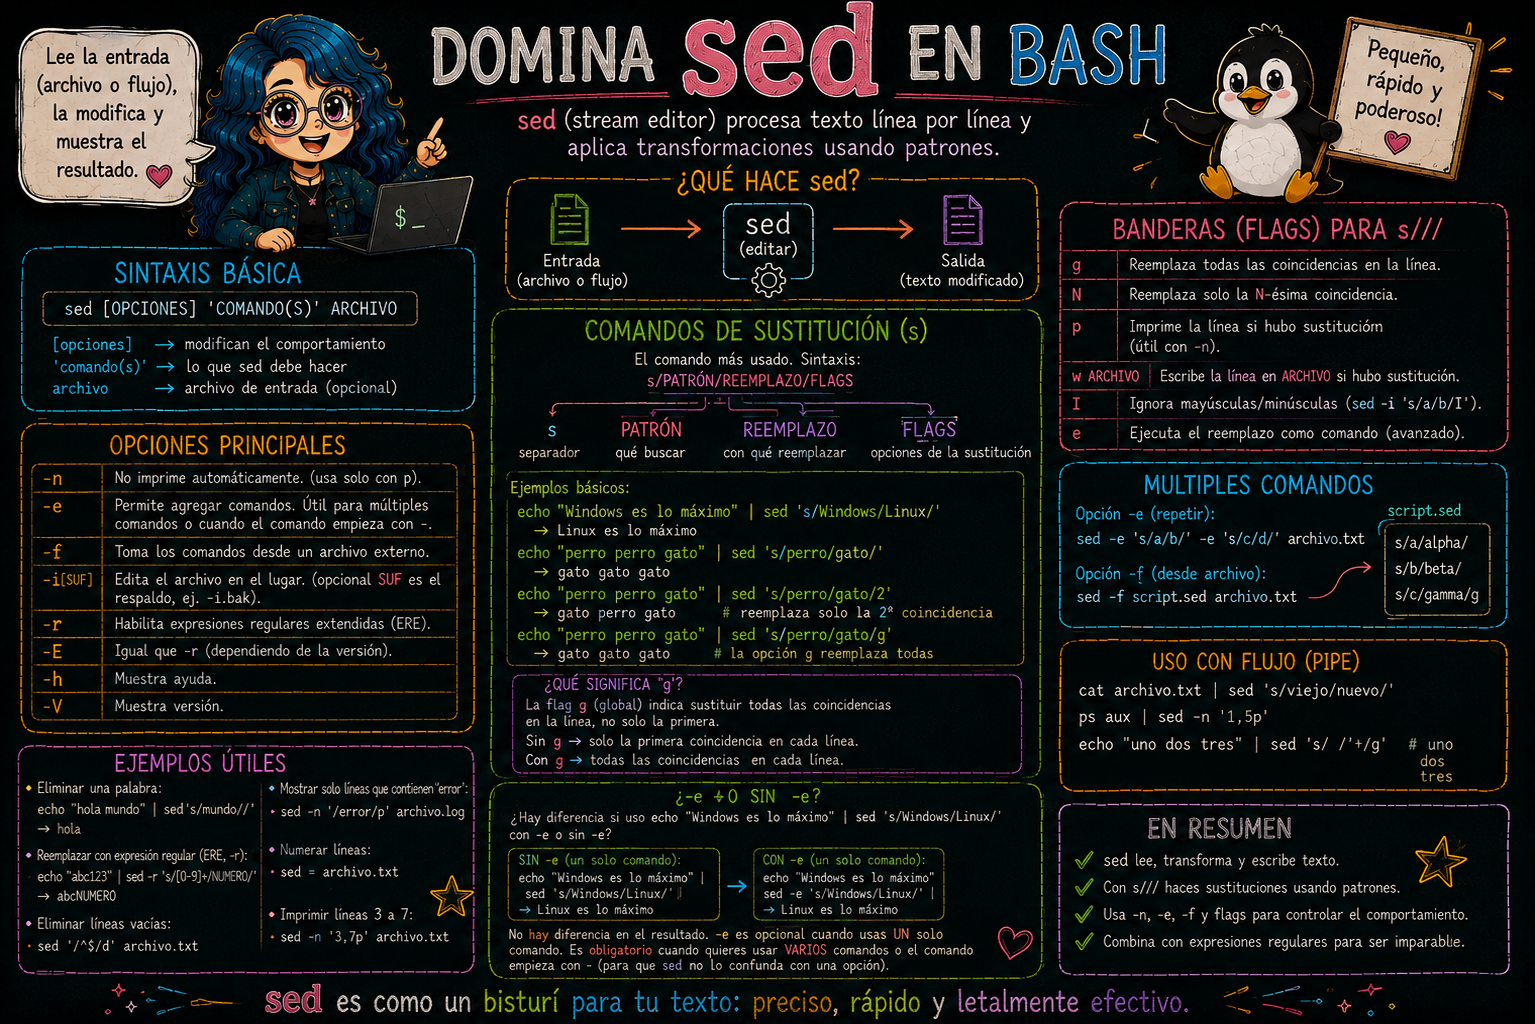
\includegraphics[keepaspectratio]{figures/bash_sed.png}}

}

\caption{Imagen creada con ChatGPT.}

\end{figure}%

\begin{tcolorbox}[enhanced jigsaw, arc=.35mm, bottomrule=.15mm, bottomtitle=1mm, breakable, colback=white, colbacktitle=quarto-callout-note-color!10!white, colframe=quarto-callout-note-color-frame, coltitle=black, left=2mm, leftrule=.75mm, opacityback=0, opacitybacktitle=0.6, rightrule=.15mm, title={Ejercicio 8: Práctica de sustituciones}, titlerule=0mm, toprule=.15mm, toptitle=1mm]

\begin{enumerate}
\def\labelenumi{\arabic{enumi}.}
\tightlist
\item
  Verifica que te encuentres en la carpeta con el comando: \texttt{pwd}
\item
  Cámbiate de carpeta si es necesario con el comando \texttt{cd}
\item
  Descarga el archivo
  \href{https://github.com/EveliaCoss/Mt2026_Taller_Computo_libro/blob/main/ejercicios/BASH/libro.txt}{\texttt{libro.txt}}
  de mi Github.
\item
  Explora este archivo con \texttt{cat\ libro.txt} ó
  \texttt{less\ libro.txt} ó \texttt{head\ libro.txt}
\item
  Sustituye la palabra ``perro'' de cada una de las filas por la palabra
  ``gato'' y una vez hecho el cambio redirige el resultado a un archivo
  llamado ``\texttt{libro\_gato.txt}''.
\item
  Corrobora tus resultados y discute posibles soluciones alternas.
\end{enumerate}

Como pudiste darte cuenta, el archivo está separado por tabulaciones
entre columna y columna. Si quisieras además, cambiar el formato del
archivo de separación por tabulaciones a separación por comas, ¿qué
pasos extra agregarías a tu código? Discute qué hace cada parte del
código.

\begin{quote}
\textbf{Solución}

\begin{Shaded}
\begin{Highlighting}[]
\FunctionTok{sed} \StringTok{\textquotesingle{}s/perro/gato/g\textquotesingle{}}\NormalTok{ libro.txt }\OperatorTok{\textgreater{}\textgreater{}}\NormalTok{ libro\_gato.txt}
\end{Highlighting}
\end{Shaded}
\end{quote}

\end{tcolorbox}

\subsection{\texorpdfstring{\texttt{sed} y las combinaciones
especiales}{sed y las combinaciones especiales}}\label{sed-y-las-combinaciones-especiales}

\begin{figure}[H]

{\centering \pandocbounded{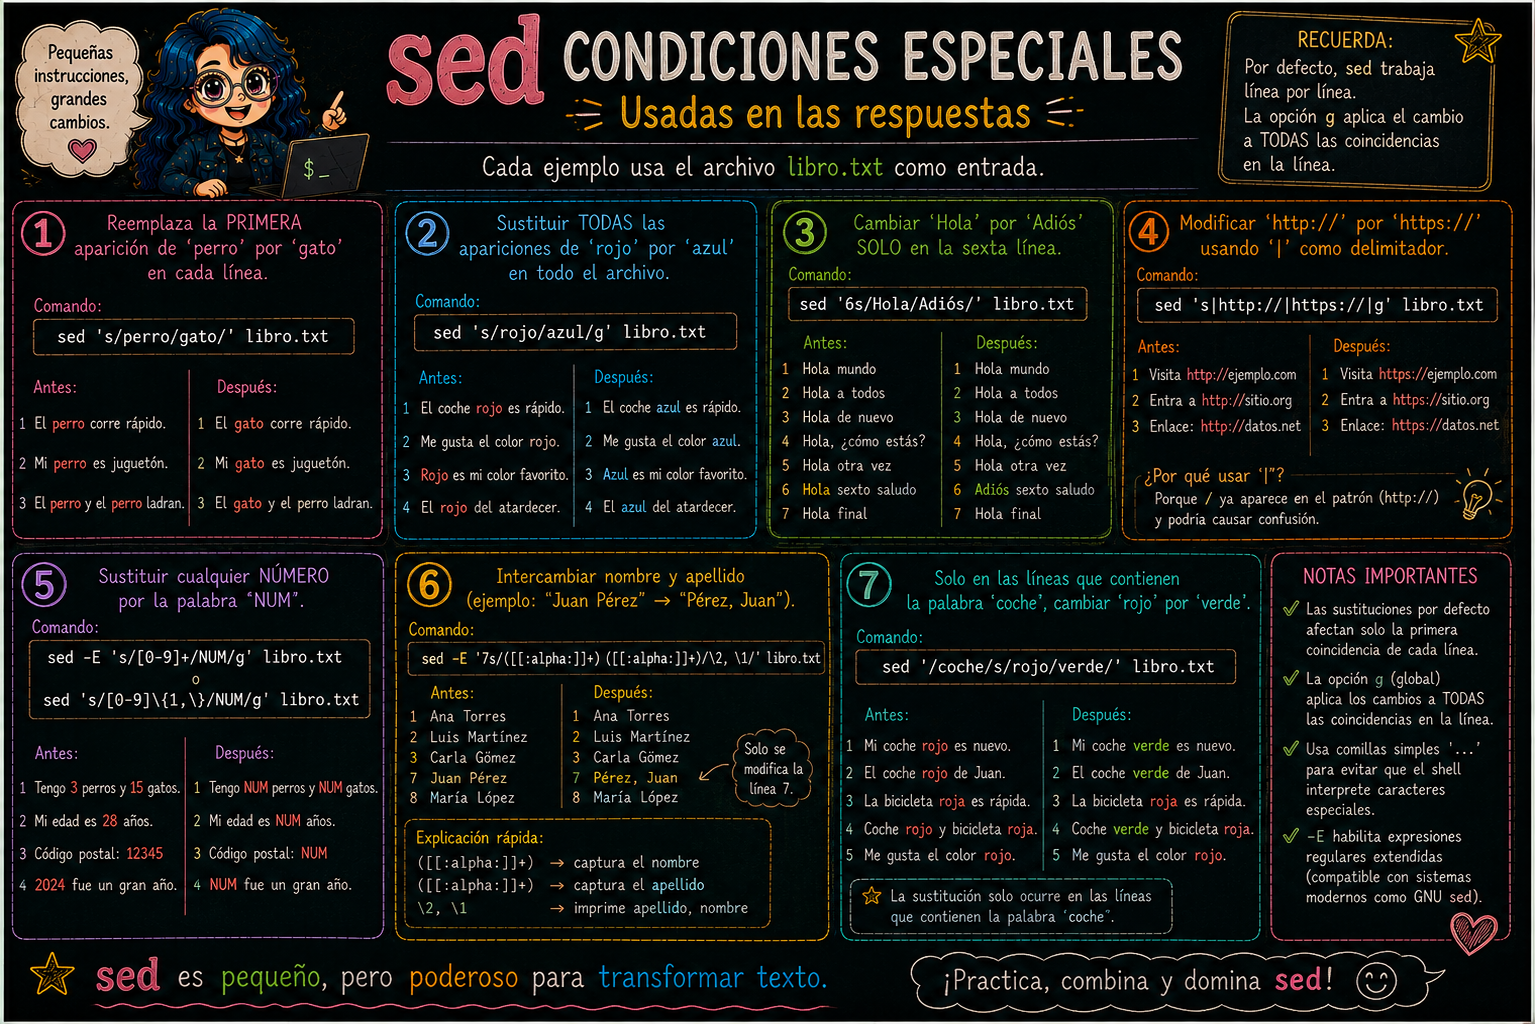
\includegraphics[keepaspectratio]{figures/bash_sed_v2.png}}

}

\caption{Imagen creada con ChatGPT.}

\end{figure}%

\begin{tcolorbox}[enhanced jigsaw, arc=.35mm, bottomrule=.15mm, bottomtitle=1mm, breakable, colback=white, colbacktitle=quarto-callout-note-color!10!white, colframe=quarto-callout-note-color-frame, coltitle=black, left=2mm, leftrule=.75mm, opacityback=0, opacitybacktitle=0.6, rightrule=.15mm, title={Ejercicio 9: Más sobre \texttt{sed}}, titlerule=0mm, toprule=.15mm, toptitle=1mm]

Seguiremos usando el contenido del archivo
\href{https://github.com/EveliaCoss/Mt2026_Taller_Computo_libro/blob/main/ejercicios/BASH/libro.txt}{\texttt{libro.txt}}
para revisar las siguientes sustituciones:

\begin{enumerate}
\def\labelenumi{\arabic{enumi}.}
\tightlist
\item
  Reemplaza la primera aparición de \texttt{perro} por \texttt{gato} en
  cada línea.
\item
  Sustituir todas las apariciones de \texttt{rojo} por \texttt{azul} en
  todo el archivo.
\item
  Cambiar \texttt{Hola} por \texttt{Adiós} solo en la sexta línea.
\item
  Modificar \texttt{http://} por \texttt{https://} usando
  \texttt{\textbar{}} como delimitador.
\item
  Sustituir cualquier número por la palabra \texttt{NUM}. NOTA: En
  \textbf{sed clásico (POSIX básico)}, el \texttt{+} no es reconocido
  como cuantificador a menos que uses la opción \texttt{-E} (o
  \texttt{-r} en GNU sed).
\item
  Intercambiar nombre y apellido (ejemplo: ``Juan Pérez'' → ``Pérez,
  Juan'').
\item
  Solo en las líneas que contienen la palabra \texttt{coche}, cambiar
  \texttt{rojo} por \texttt{verde.}
\end{enumerate}

\begin{quote}
\textbf{Solución}

\begin{Shaded}
\begin{Highlighting}[]
\ExtensionTok{1.}\NormalTok{ sed }\StringTok{\textquotesingle{}s/perro/gato/\textquotesingle{}}\NormalTok{ libro.txt}
\ExtensionTok{2.}\NormalTok{ sed }\StringTok{\textquotesingle{}s/rojo/azul/g\textquotesingle{}}\NormalTok{ libro.txt}
\ExtensionTok{3.}\NormalTok{ sed }\StringTok{\textquotesingle{}6s/Hola/Adiós/\textquotesingle{}}\NormalTok{ libro.txt}
\ExtensionTok{4.}\NormalTok{ sed }\StringTok{\textquotesingle{}s|http://|https://|g\textquotesingle{}}\NormalTok{ libro.txt}
\ExtensionTok{5.}\NormalTok{ sed }\AttributeTok{{-}E} \StringTok{\textquotesingle{}s/[0{-}9]+/NUM/g\textquotesingle{}}\NormalTok{ libro.txt o sed }\StringTok{\textquotesingle{}s/[0{-}9]\textbackslash{}\{1,\textbackslash{}\}/NUM/g\textquotesingle{}}\NormalTok{ libro.txt }\CommentTok{\# La sintaxis \textbackslash{}\{n,m\textbackslash{}\} indica cuántas veces debe repetirse el patrón anterior.}
\ExtensionTok{6.}\NormalTok{ sed }\AttributeTok{{-}E} \StringTok{\textquotesingle{}7s/([[:alpha:]]+) ([[:alpha:]]+)/\textbackslash{}2, \textbackslash{}1/\textquotesingle{}}\NormalTok{ libro.txt }
\ExtensionTok{7.}\NormalTok{ sed }\StringTok{\textquotesingle{}/coche/s/rojo/verde/\textquotesingle{}}\NormalTok{ libro.txt}
\end{Highlighting}
\end{Shaded}
\end{quote}

\end{tcolorbox}

\pandocbounded{\includegraphics[keepaspectratio]{figures/nac35ntlfg831.webp}}

\subsection{Referencias}\label{referencias-6}

\begin{itemize}
\tightlist
\item
  \href{https://www.rexegg.com/regex-quickstart.php}{RegEx}
\item
  \href{https://es.wikipedia.org/wiki/Expresi\%C3\%B3n_regular}{Wikipedia:
  Expresiones Regulares}
\item
  \href{https://www.youtube.com/watch?v=OIxDMnBp-2g}{YouTube:
  Expresiones regulares con Notepad++}
\end{itemize}

\chapter{Tipos de enlaces - symlinks, hard links e
hipervínculos}\label{tipos-de-enlaces---symlinks-hard-links-e-hipervuxednculos}

\begin{quote}
\textbf{Fecha:} 24 de septiembre, 2026
\end{quote}

Es mejor crear \textbf{enlaces simbólicos (symlinks)} en vez de copiar
cada archivo, ya que permite ahorrar mucho espacio en el disco al evitar
la multiplicación de copias fisicas en el disco duro del mismo archivo.

Una modificación realizada utilizando este enlace se reflejará en el
original; pero, por el contrario, si se elimina el enlace, no se
eliminará el auténtico.

\section{Diferencias entre enlaces simbólicos (symlinks) y enlaces duros
(hard
links)}\label{diferencias-entre-enlaces-simbuxf3licos-symlinks-y-enlaces-duros-hard-links}

{\def\LTcaptype{none} % do not increment counter
\begin{longtable}[]{@{}
  >{\raggedright\arraybackslash}p{(\linewidth - 4\tabcolsep) * \real{0.1246}}
  >{\raggedright\arraybackslash}p{(\linewidth - 4\tabcolsep) * \real{0.4058}}
  >{\raggedright\arraybackslash}p{(\linewidth - 4\tabcolsep) * \real{0.4665}}@{}}
\toprule\noalign{}
\begin{minipage}[b]{\linewidth}\raggedright
Características
\end{minipage} & \begin{minipage}[b]{\linewidth}\raggedright
Symlinks
\end{minipage} & \begin{minipage}[b]{\linewidth}\raggedright
Hard links
\end{minipage} \\
\midrule\noalign{}
\endhead
\bottomrule\noalign{}
\endlastfoot
\textbf{Almacenamiento} & \begin{minipage}[t]{\linewidth}\raggedright
\begin{itemize}
\tightlist
\item
  Actúa como un puntero o referencia a otro archivo o directorio.
\item
  No contiene los datos reales del archivo, sino una tuta que apunta al
  archivo original.
\end{itemize}
\end{minipage} & \begin{minipage}[t]{\linewidth}\raggedright
\begin{itemize}
\item
  Apunta directamente a los datos del archivo original.
\item
  Comparte el mismo contenido que el archivo enlazado, no solo una
  referencia.
\end{itemize}
\end{minipage} \\
\textbf{Número de inodo} & Cuenta con un número de inodo (nodo indice)
diferente del archivo original. Se identifica como un tipo de archivo
diferente. & Comparte el mismo número de inodo con el destino. Elimina
el concepto de ``archivo original''; todos los hard links al mismo
archivo son iguales. \\
\textbf{Eliminación del archivo original} & Si el archivo original se
elimina, el symlink queda roto (es decir, apunta a algo inexistente). &
Si un hard link se elimina, los datos del archivo permanecen accesibles
mientras existan otros hard links. \\
\textbf{Sistema de archivos.} & Puede apuntar a archivos o directorios,
incluso en diferentes sistemas de archivos. & Deben residir en el mismo
sistema de archivos. \\
\textbf{Rutas} & Se pueden usar rutas absolutas o relativas para la
referencia. & No puede enlazar directorios (en la mayoría de los
sistemas modernos) ni cruzar sistemas de archivos diferentes. \\
\textbf{Uso común} & \begin{minipage}[t]{\linewidth}\raggedright
\begin{itemize}
\tightlist
\item
  Crear accesos directos a archivos o carpetas.
\item
  Facilitar la gestión de rutas en aplicaciones.
\end{itemize}
\end{minipage} & \begin{minipage}[t]{\linewidth}\raggedright
\begin{itemize}
\tightlist
\item
  Garantizar accesibilidad a datos independientemente de qué enlace se
  elimine.
\item
  Compartir archivos de forma eficiente sin duplicar espacio en disco.
\end{itemize}
\end{minipage} \\
\textbf{Comando para crear} &
\begin{minipage}[t]{\linewidth}\raggedright
\begin{Shaded}
\begin{Highlighting}[]
\FunctionTok{ln} \AttributeTok{{-}s}\NormalTok{ archivo\_original enlace\_simbolico}
\end{Highlighting}
\end{Shaded}
\end{minipage} & \begin{minipage}[t]{\linewidth}\raggedright
\begin{Shaded}
\begin{Highlighting}[]
\FunctionTok{ln}\NormalTok{ archivo\_original enlace\_simbolico}
\end{Highlighting}
\end{Shaded}
\end{minipage} \\
\end{longtable}
}

\begin{tcolorbox}[enhanced jigsaw, arc=.35mm, bottomrule=.15mm, bottomtitle=1mm, breakable, colback=white, colbacktitle=quarto-callout-caution-color!10!white, colframe=quarto-callout-caution-color-frame, coltitle=black, left=2mm, leftrule=.75mm, opacityback=0, opacitybacktitle=0.6, rightrule=.15mm, title=\textcolor{quarto-callout-caution-color}{\faFire}\hspace{0.5em}{Precaución}, titlerule=0mm, toprule=.15mm, toptitle=1mm]

Debes tener cuidado al elegir cuál utilizar. Los \textbf{enlaces
simbólicos} son más convenientes cuando trabajamos con datos importantes
que están almacenados en un respaldo, ya que permiten acceder fácilmente
a los archivos originales sin duplicarlos y facilitan la gestión de
rutas, sin eliminar o afectar los archivos originales.

\end{tcolorbox}

\begin{figure}[H]

{\centering \pandocbounded{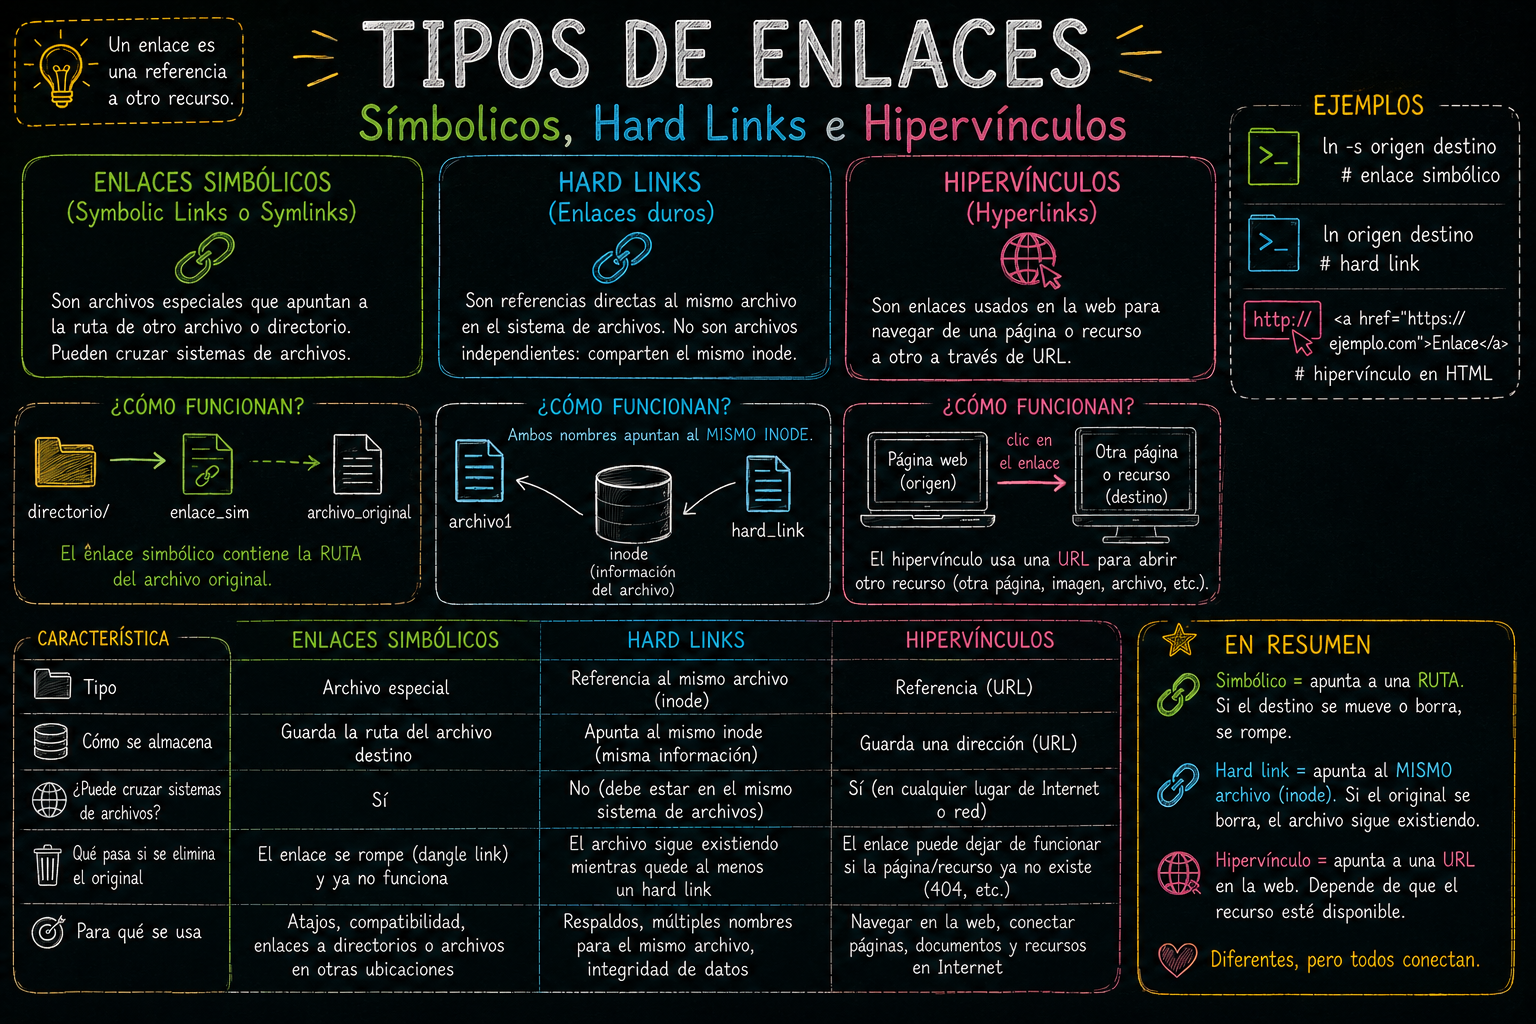
\includegraphics[keepaspectratio]{figures/bash_enlaces.png}}

}

\caption{Imagen creada con ChatGPT.}

\end{figure}%

\section{Orden de los archivos}\label{orden-de-los-archivos}

El \textbf{sistema de archivos de GNU/Linux} tiene una estructura
jerárquica de directorios y subdirectorios que penden del
\textbf{directorio raíz} \texttt{/}. Esta estructura puede ser
visualizada convenientemente con el comando \texttt{tree} (Nota:
\texttt{tree} tal vez no esté instalado en tu sistema).

Organizar tu entorno de trabajo en \textbf{Bash} siguiendo buenas
prácticas te permitirá gestionar tus archivos y scripts de manera
eficiente. Aquí tienes una sugerencia de carpetas clave y nombres que
puedes utilizar:

\begin{verbatim}
~/workspace/
├── bin/           # Scripts ejecutables
├── src/           # Código fuente
├── logs/          # Archivos de registro
├── config/        # Configuración
├── data/
│   ├── raw/       # Datos crudos
│   └── processed/ # Datos procesados
├── backup/        # Copias de seguridad
├── tmp/           # Archivos temporales
├── projects/
│   └── project_name/
├── git/           # Repositorios locales
└── docs/          # Documentación
\end{verbatim}

\subsection{\texorpdfstring{\textbf{Consejos
adicionales}}{Consejos adicionales}}\label{consejos-adicionales}

\begin{enumerate}
\def\labelenumi{\arabic{enumi}.}
\item
  \textbf{Usa nombres descriptivos:} Los nombres de las carpetas y
  archivos deben reflejar su contenido claramente.
\item
  \textbf{Mantén consistencia:} Usa un esquema de nombres uniforme (por
  ejemplo, todo en minúsculas o con guiones bajos).
\item
  \textbf{Automatiza la limpieza:} Utiliza scripts en Bash para eliminar
  archivos temporales o rotar logs antiguos.
\item
  \textbf{Usa control de versiones:} Integra Git en tus proyectos para
  mantener un historial de cambios en tus scripts.
\end{enumerate}

Esta estructura es flexible y se puede ajustar según tus necesidades
específicas.

\section{Referencias}\label{referencias-7}

\begin{itemize}
\item
  \href{https://www.hostinger.com/tutorials/how-to-create-symbolic-links-in-linux/?utm_campaign=Generic-Tutorials-DSA\%7CNT:Se\%7CLO:MX-EN&utm_medium=ppc&gad_source=1&gclid=Cj0KCQiAu8W6BhC-ARIsACEQoDBS5S76IeOtxlAtbyI5wPmsI72ILku8waMvXKlUo0X-ZzddJpjvKSAaAuAiEALw_wcB}{How
  to create and remove Linux symlinks for files and directories}
\item
  \href{https://vinuesa.github.io/intro2linux/index.html\#generaci\%C3\%B3n-de-ligas-simb\%C3\%B3licas-a-archivos-comando-ln--s-rutaalarchivofuente-nombre_liga}{Generación
  de ligas simbólicas a archivos: comando \textbf{ln -s
  /ruta/al/archivo/fuente nombre\_liga}}
\end{itemize}

\chapter{\texorpdfstring{Filtrado de texto
(\texttt{grep,\ cut,\ sort,\ uniq,\ wc})}{Filtrado de texto (grep, cut, sort, uniq, wc)}}\label{filtrado-de-texto-grep-cut-sort-uniq-wc}

\begin{quote}
\textbf{Fecha:} 29 de septiembre, 2026
\end{quote}

\begin{tcolorbox}[enhanced jigsaw, arc=.35mm, bottomrule=.15mm, bottomtitle=1mm, breakable, colback=white, colbacktitle=quarto-callout-warning-color!10!white, colframe=quarto-callout-warning-color-frame, coltitle=black, left=2mm, leftrule=.75mm, opacityback=0, opacitybacktitle=0.6, rightrule=.15mm, title=\textcolor{quarto-callout-warning-color}{\faExclamationTriangle}\hspace{0.5em}{En proceso de desarrollo}, titlerule=0mm, toprule=.15mm, toptitle=1mm]

\end{tcolorbox}

Veamos ahora los comandos más usados en \textbf{pipelines o tuberías} de
filtrado de texto en acción, haciendo uso de sólo algunas de las
opciones más frecuentes listados en la sección anterior.

\begin{tcolorbox}[enhanced jigsaw, arc=.35mm, bottomrule=.15mm, bottomtitle=1mm, breakable, colback=white, colbacktitle=quarto-callout-important-color!10!white, colframe=quarto-callout-important-color-frame, coltitle=black, left=2mm, leftrule=.75mm, opacityback=0, opacitybacktitle=0.6, rightrule=.15mm, title=\textcolor{quarto-callout-important-color}{\faExclamation}\hspace{0.5em}{Importante}, titlerule=0mm, toprule=.15mm, toptitle=1mm]

La filosofía de un \textbf{pipeline o tubería} en Bash es que \textbf{la
salida de un comando se convierte en la entrada del siguiente mediante
\texttt{\textbar{}} (pipe)}.

\end{tcolorbox}

Al final de esta clase podrás leer comandos como estos:

\begin{Shaded}
\begin{Highlighting}[]
\FunctionTok{grep} \StringTok{"Aprobado"}\NormalTok{ calificaciones.txt }\KeywordTok{|} \FunctionTok{cut} \AttributeTok{{-}d}\StringTok{\textquotesingle{},\textquotesingle{}} \AttributeTok{{-}f2} \KeywordTok{|} \FunctionTok{sort} \KeywordTok{|} \FunctionTok{uniq} \AttributeTok{{-}c} \KeywordTok{|} \FunctionTok{sort} \AttributeTok{{-}nr}
\end{Highlighting}
\end{Shaded}

No necesariamente memorizarlo de golpe, sino entender \textbf{qué aporta
cada etapa}:

{\def\LTcaptype{none} % do not increment counter
\begin{longtable}[]{@{}ll@{}}
\toprule\noalign{}
Comando & ¿Para qué sirve? \\
\midrule\noalign{}
\endhead
\bottomrule\noalign{}
\endlastfoot
\texttt{grep} & Buscar patrones en texto \\
\texttt{cut} & Extraer columnas o campos \\
\texttt{sort} & Ordenar líneas \\
\texttt{uniq} & Eliminar/contar duplicados \\
\texttt{wc} & Contar líneas, palabras y caracteres \\
\end{longtable}
}

Podemos crear 3 archivos:

\begin{enumerate}
\def\labelenumi{\arabic{enumi}.}
\tightlist
\item
  El archivo \texttt{nombres.txt}:
\end{enumerate}

\begin{Shaded}
\begin{Highlighting}[]
\BuiltInTok{echo} \AttributeTok{{-}e} \StringTok{"Sofía\textbackslash{}nCarlos\textbackslash{}nAna\textbackslash{}nMiguel\textbackslash{}nElena\textbackslash{}nDiego\textbackslash{}nBeatriz\textbackslash{}nFernando\textbackslash{}nLaura\textbackslash{}nJorge"} \OperatorTok{\textgreater{}}\NormalTok{ ejercicios/BASH/nombres.txt}
\end{Highlighting}
\end{Shaded}

\begin{enumerate}
\def\labelenumi{\arabic{enumi}.}
\setcounter{enumi}{1}
\tightlist
\item
  El archivo \texttt{numeros.txt}:
\end{enumerate}

\begin{Shaded}
\begin{Highlighting}[]
\BuiltInTok{echo} \AttributeTok{{-}e} \StringTok{"42\textbackslash{}n7\textbackslash{}n100\textbackslash{}n23\textbackslash{}n5\textbackslash{}n81\textbackslash{}n16\textbackslash{}n3\textbackslash{}n55\textbackslash{}n12"} \OperatorTok{\textgreater{}}\NormalTok{ ejercicios/BASH/numeros.txt}
\end{Highlighting}
\end{Shaded}

\begin{enumerate}
\def\labelenumi{\arabic{enumi}.}
\setcounter{enumi}{2}
\tightlist
\item
  El archivo \texttt{datos.txt}:
\end{enumerate}

\begin{Shaded}
\begin{Highlighting}[]
\BuiltInTok{echo} \AttributeTok{{-}e} \StringTok{"Ana 85\textbackslash{}nLuis 72\textbackslash{}nMaría 94\textbackslash{}nCarlos 68\textbackslash{}nSofía 91\textbackslash{}nDiego 77\textbackslash{}nElena 88\textbackslash{}nPablo 63"} \OperatorTok{\textgreater{}}\NormalTok{ ejercicios/BASH/datos.txt}
\end{Highlighting}
\end{Shaded}

\begin{enumerate}
\def\labelenumi{\arabic{enumi}.}
\setcounter{enumi}{3}
\tightlist
\item
  El archivo \texttt{temas.txt}:
\end{enumerate}

\begin{Shaded}
\begin{Highlighting}[]
\BuiltInTok{echo} \AttributeTok{{-}e} \StringTok{"Álgebra\textbackslash{}nCálculo\textbackslash{}nÁlgebra\textbackslash{}nGeometría\textbackslash{}nCálculo\textbackslash{}nÁlgebra\textbackslash{}nEstadística"} \OperatorTok{\textgreater{}}\NormalTok{ ejercicios/BASH/temas.txt}
\end{Highlighting}
\end{Shaded}

\begin{enumerate}
\def\labelenumi{\arabic{enumi}.}
\setcounter{enumi}{4}
\tightlist
\item
  El archivo \texttt{alumnos.txt}:
\end{enumerate}

\begin{Shaded}
\begin{Highlighting}[]
\BuiltInTok{echo} \AttributeTok{{-}e} \StringTok{"Ana:85:Álgebra\textbackslash{}nLuis:72:Cálculo\textbackslash{}nMaría:94:Estadística\textbackslash{}nCarlos:68:Geometría\textbackslash{}nSofía:91:Cálculo"} \OperatorTok{\textgreater{}}\NormalTok{ ejercicios/BASH/alumnos.txt}
\end{Highlighting}
\end{Shaded}

\section{\texorpdfstring{Repaso de \texttt{grep} - Buscar patrones en
texto}{Repaso de grep - Buscar patrones en texto}}\label{repaso-de-grep---buscar-patrones-en-texto}

\textbf{Sintaxis:}

\begin{verbatim}
grep [opciones] "patrón" archivo
\end{verbatim}

{\def\LTcaptype{none} % do not increment counter
\begin{longtable}[]{@{}
  >{\raggedright\arraybackslash}p{(\linewidth - 4\tabcolsep) * \real{0.1333}}
  >{\raggedright\arraybackslash}p{(\linewidth - 4\tabcolsep) * \real{0.4778}}
  >{\raggedright\arraybackslash}p{(\linewidth - 4\tabcolsep) * \real{0.3778}}@{}}
\toprule\noalign{}
\begin{minipage}[b]{\linewidth}\raggedright
Argumento
\end{minipage} & \begin{minipage}[b]{\linewidth}\raggedright
Descripción
\end{minipage} & \begin{minipage}[b]{\linewidth}\raggedright
Ejemplo
\end{minipage} \\
\midrule\noalign{}
\endhead
\bottomrule\noalign{}
\endlastfoot
& & \begin{minipage}[t]{\linewidth}\raggedright
\begin{Shaded}
\begin{Highlighting}[]
\FunctionTok{grep} \StringTok{":[9][0{-}9]:"}\NormalTok{ alumnos.txt}
\end{Highlighting}
\end{Shaded}
\end{minipage} \\
\texttt{-i} & Ignora mayúsculas y minúsculas &
\begin{minipage}[t]{\linewidth}\raggedright
\begin{Shaded}
\begin{Highlighting}[]
\FunctionTok{grep} \AttributeTok{{-}i} \StringTok{"carlos"}\NormalTok{ nombres.txt}
\end{Highlighting}
\end{Shaded}
\end{minipage} \\
\texttt{-n} & Muestra el número de línea &
\begin{minipage}[t]{\linewidth}\raggedright
\begin{Shaded}
\begin{Highlighting}[]
\FunctionTok{grep} \AttributeTok{{-}n} \StringTok{"Miguel"}\NormalTok{ nombres.txt}
\end{Highlighting}
\end{Shaded}
\end{minipage} \\
\texttt{-c} & Cuenta las líneas que coinciden &
\begin{minipage}[t]{\linewidth}\raggedright
\begin{Shaded}
\begin{Highlighting}[]
\FunctionTok{grep} \AttributeTok{{-}c} \StringTok{"Cálculo"}\NormalTok{alumnos.txt}
\end{Highlighting}
\end{Shaded}
\end{minipage} \\
\texttt{-v} & Muestra líneas que \textbf{NO} coinciden &
\begin{minipage}[t]{\linewidth}\raggedright
\begin{Shaded}
\begin{Highlighting}[]
\FunctionTok{grep} \AttributeTok{{-}v} \StringTok{"a"}\NormalTok{ nombres.txt}
\FunctionTok{grep} \AttributeTok{{-}v} \StringTok{"Cálculo"}\NormalTok{ alumnos.txt}
\end{Highlighting}
\end{Shaded}
\end{minipage} \\
\texttt{-w} & Coincidencia de palabra completa &
\begin{minipage}[t]{\linewidth}\raggedright
\begin{Shaded}
\begin{Highlighting}[]
\FunctionTok{grep} \AttributeTok{{-}w} \StringTok{"Cálculo"}\NormalTok{ alumnos.txt}
\end{Highlighting}
\end{Shaded}
\end{minipage} \\
\texttt{-A\ n} & Muestra \texttt{n} líneas \textbf{después} del match &
\begin{minipage}[t]{\linewidth}\raggedright
\begin{Shaded}
\begin{Highlighting}[]
\FunctionTok{grep} \AttributeTok{{-}A}\NormalTok{ 2 }\StringTok{"Álgebra"}\NormalTok{ alumnos.txt}
\end{Highlighting}
\end{Shaded}
\end{minipage} \\
\end{longtable}
}

Durante la clase de
\href{https://eveliacoss.github.io/Mt2026_Taller_Computo_libro/cap7.html}{``Encontrar
patrones con grep''} repasamos la siguiente infografía y realizamos
algunos ejercicios.

\begin{figure}[H]

{\centering \pandocbounded{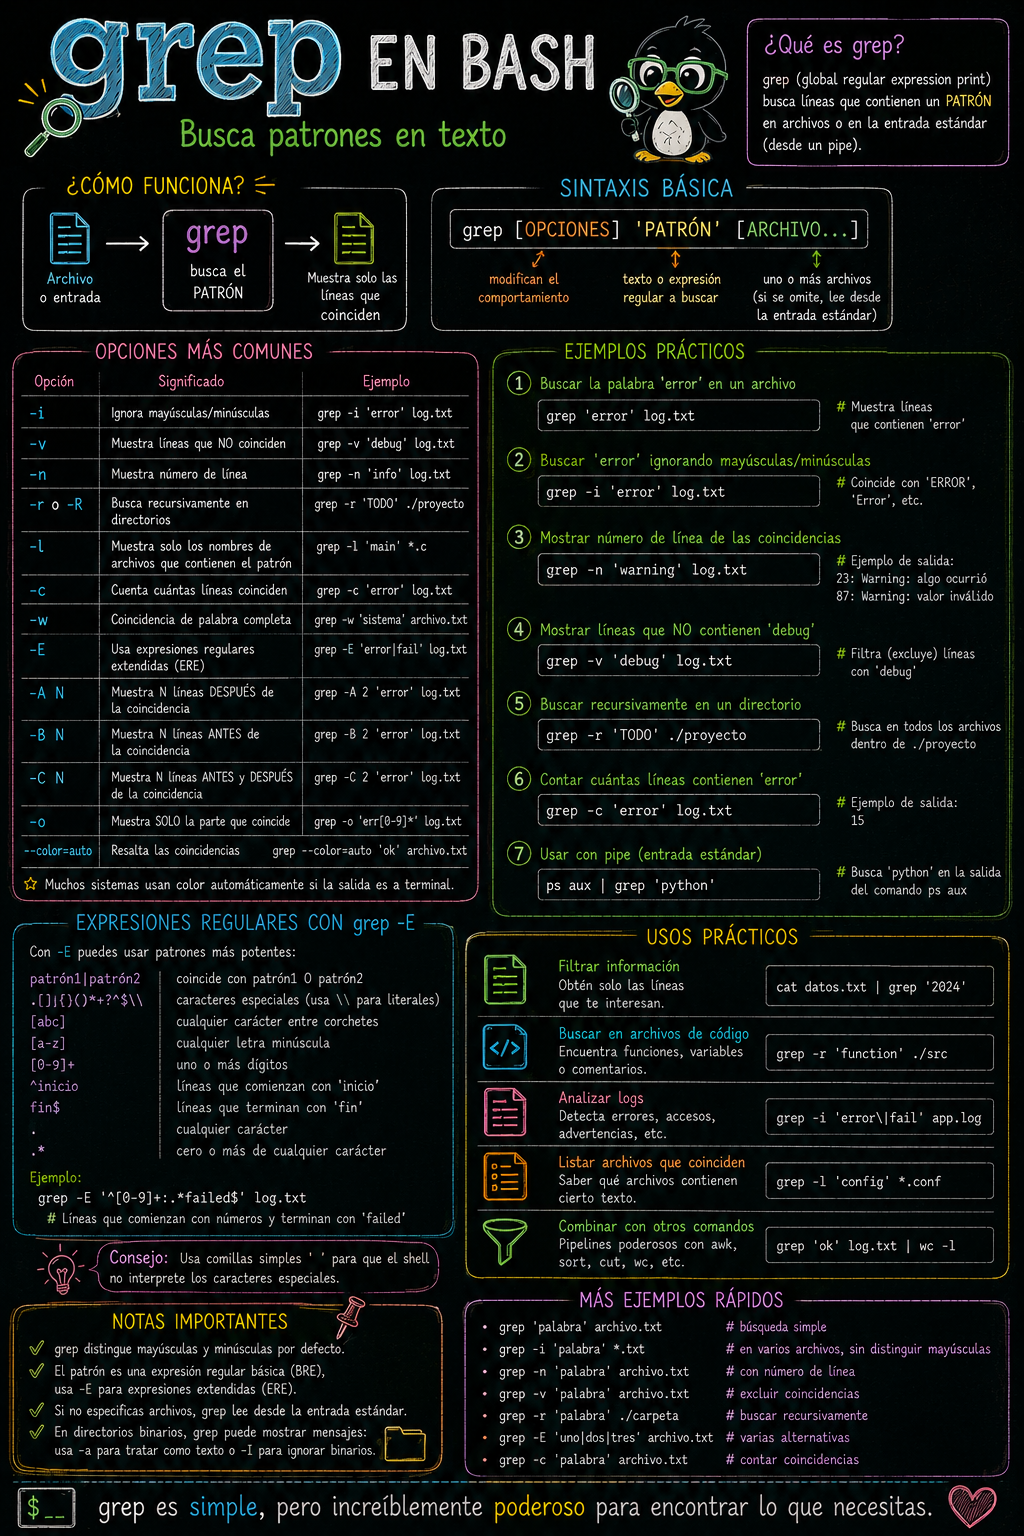
\includegraphics[keepaspectratio]{figures/bash_grep.png}}

}

\caption{Infografía de grep - creada con ChatGPT}

\end{figure}%

\section{\texorpdfstring{\texttt{sort} - Ordenar líneas de
texto}{sort - Ordenar líneas de texto}}\label{sort---ordenar-luxedneas-de-texto}

\textbf{Sintaxis:}

\begin{verbatim}
sort [opciones] archivo.txt
\end{verbatim}

{\def\LTcaptype{none} % do not increment counter
\begin{longtable}[]{@{}
  >{\raggedright\arraybackslash}p{(\linewidth - 4\tabcolsep) * \real{0.1481}}
  >{\raggedright\arraybackslash}p{(\linewidth - 4\tabcolsep) * \real{0.4691}}
  >{\raggedright\arraybackslash}p{(\linewidth - 4\tabcolsep) * \real{0.3704}}@{}}
\toprule\noalign{}
\begin{minipage}[b]{\linewidth}\raggedright
Argumento
\end{minipage} & \begin{minipage}[b]{\linewidth}\raggedright
Descripción
\end{minipage} & \begin{minipage}[b]{\linewidth}\raggedright
Ejemplo
\end{minipage} \\
\midrule\noalign{}
\endhead
\bottomrule\noalign{}
\endlastfoot
& Orden alfabético & \begin{minipage}[t]{\linewidth}\raggedright
\begin{Shaded}
\begin{Highlighting}[]
\FunctionTok{sort}\NormalTok{ nombres.txt}
\FunctionTok{sort}\NormalTok{ temas.txt}
\end{Highlighting}
\end{Shaded}
\end{minipage} \\
\texttt{-n} & Ordena numéricamente &
\begin{minipage}[t]{\linewidth}\raggedright
\begin{Shaded}
\begin{Highlighting}[]
\FunctionTok{sort} \AttributeTok{{-}n}\NormalTok{ numeros.txt}
\end{Highlighting}
\end{Shaded}
\end{minipage} \\
\texttt{-r} & Orden inverso (descendente) &
\begin{minipage}[t]{\linewidth}\raggedright
\begin{Shaded}
\begin{Highlighting}[]
\FunctionTok{sort} \AttributeTok{{-}r}\NormalTok{ numeros.txt}
\end{Highlighting}
\end{Shaded}
\end{minipage} \\
\texttt{-k} & Ordena por columna específica &
\begin{minipage}[t]{\linewidth}\raggedright
\begin{Shaded}
\begin{Highlighting}[]
\FunctionTok{sort} \AttributeTok{{-}k2}\NormalTok{ datos.txt}
\FunctionTok{sort} \AttributeTok{{-}k2nr}\NormalTok{ datos.txt}
\end{Highlighting}
\end{Shaded}
\end{minipage} \\
\texttt{-u} & Elimina duplicados mientras ordena &
\begin{minipage}[t]{\linewidth}\raggedright
\begin{Shaded}
\begin{Highlighting}[]
\FunctionTok{sort} \AttributeTok{{-}u}\NormalTok{ temas.txt}
\end{Highlighting}
\end{Shaded}
\end{minipage} \\
\texttt{-t} & Define separador de campos/columnas &
\begin{minipage}[t]{\linewidth}\raggedright
\begin{Shaded}
\begin{Highlighting}[]
\FunctionTok{sort} \AttributeTok{{-}t}\StringTok{":"} \AttributeTok{{-}k2n}\NormalTok{ alumnos.txt}
\FunctionTok{sort} \AttributeTok{{-}t}\StringTok{":"} \AttributeTok{{-}k3}\NormalTok{ alumnos.txt}
\end{Highlighting}
\end{Shaded}
\end{minipage} \\
\end{longtable}
}

\begin{figure}[H]

{\centering \pandocbounded{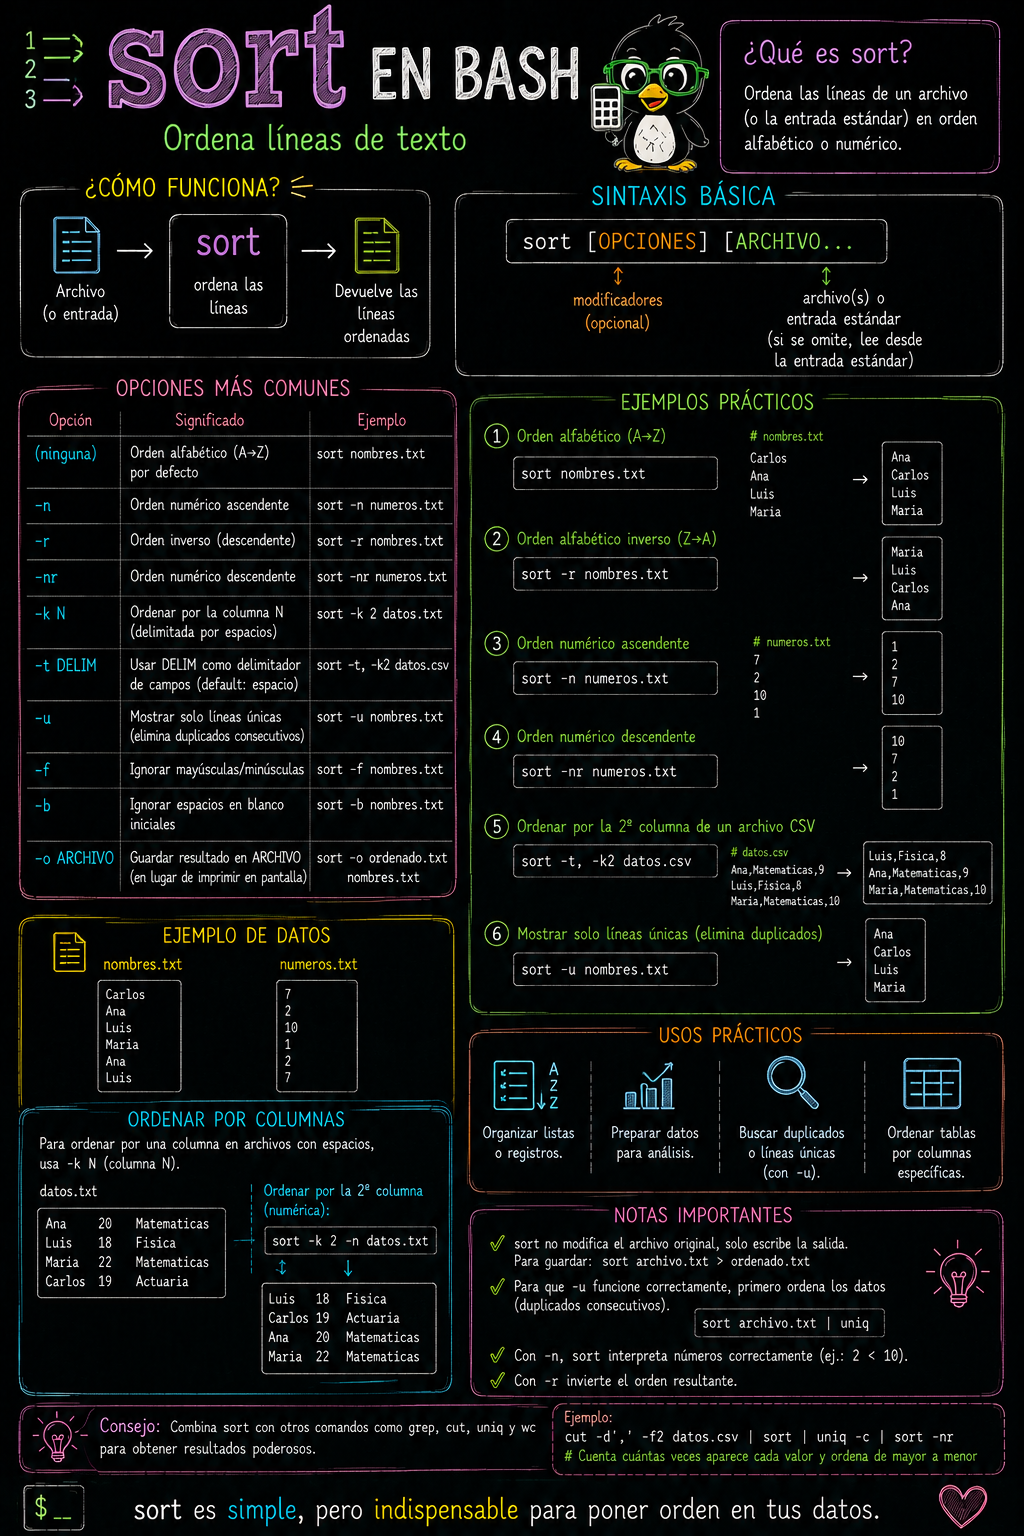
\includegraphics[keepaspectratio]{figures/bash_sort.png}}

}

\caption{Imagen creada con ChatGPT.}

\end{figure}%

\section{\texorpdfstring{\texttt{uniq} - Identifica y filtra líneas
repetidas}{uniq - Identifica y filtra líneas repetidas}}\label{uniq---identifica-y-filtra-luxedneas-repetidas}

\textbf{Sintaxis:}

\begin{verbatim}
uniq [opciones] archivo.txt
\end{verbatim}

{\def\LTcaptype{none} % do not increment counter
\begin{longtable}[]{@{}
  >{\raggedright\arraybackslash}p{(\linewidth - 4\tabcolsep) * \real{0.1558}}
  >{\raggedright\arraybackslash}p{(\linewidth - 4\tabcolsep) * \real{0.4545}}
  >{\raggedright\arraybackslash}p{(\linewidth - 4\tabcolsep) * \real{0.3766}}@{}}
\toprule\noalign{}
\begin{minipage}[b]{\linewidth}\raggedright
Argumento
\end{minipage} & \begin{minipage}[b]{\linewidth}\raggedright
Descripción
\end{minipage} & \begin{minipage}[b]{\linewidth}\raggedright
Ejemplo
\end{minipage} \\
\midrule\noalign{}
\endhead
\bottomrule\noalign{}
\endlastfoot
& Ordena y elimina duplicado &
\begin{minipage}[t]{\linewidth}\raggedright
\begin{Shaded}
\begin{Highlighting}[]
\FunctionTok{sort}\NormalTok{ temas.txt }\KeywordTok{|} \FunctionTok{uniq}
\end{Highlighting}
\end{Shaded}
\end{minipage} \\
\texttt{-c} & Cuenta ocurrencias de cada línea &
\begin{minipage}[t]{\linewidth}\raggedright
\begin{Shaded}
\begin{Highlighting}[]
\FunctionTok{sort}\NormalTok{ datos.txt }\KeywordTok{|} \FunctionTok{uniq} \AttributeTok{{-}c}
\end{Highlighting}
\end{Shaded}
\end{minipage} \\
\texttt{-d} & Muestra solo líneas duplicadas &
\begin{minipage}[t]{\linewidth}\raggedright
\begin{Shaded}
\begin{Highlighting}[]
\FunctionTok{sort}\NormalTok{ datos.txt }\KeywordTok{|} \FunctionTok{uniq} \AttributeTok{{-}d}
\end{Highlighting}
\end{Shaded}
\end{minipage} \\
\texttt{-u} & Muestra solo líneas únicas &
\begin{minipage}[t]{\linewidth}\raggedright
\begin{Shaded}
\begin{Highlighting}[]
\FunctionTok{sort}\NormalTok{ datos.txt }\KeywordTok{|} \FunctionTok{uniq} \AttributeTok{{-}u}
\end{Highlighting}
\end{Shaded}
\end{minipage} \\
\end{longtable}
}

\begin{figure}[H]

{\centering \pandocbounded{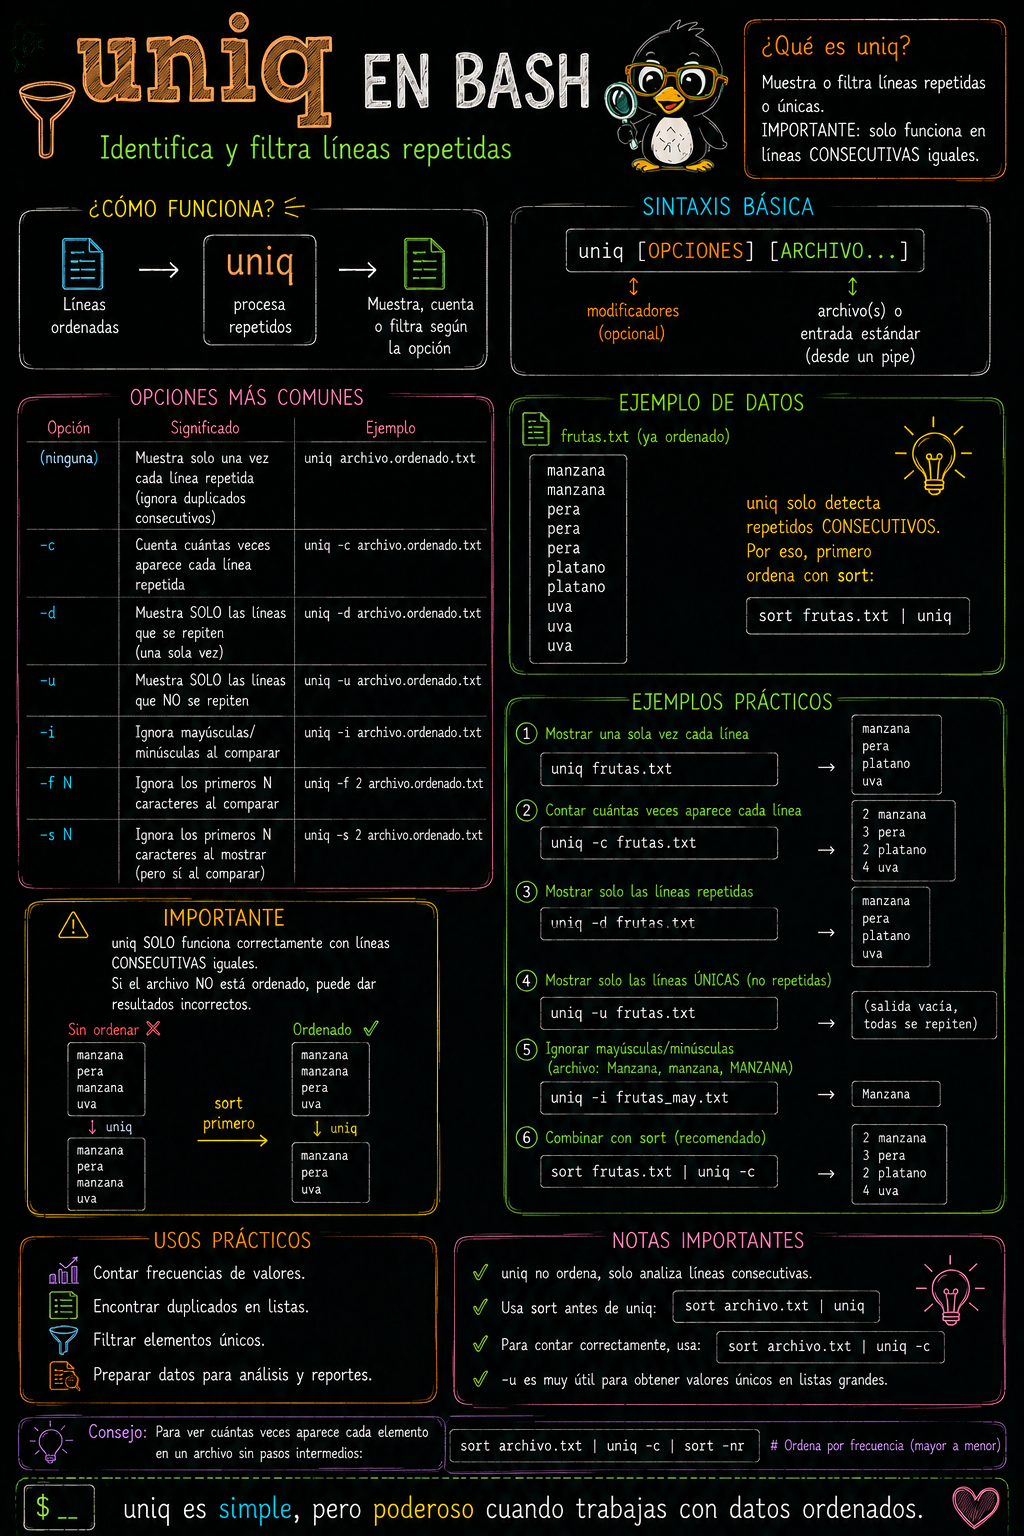
\includegraphics[keepaspectratio]{figures/bash_uniq.png}}

}

\caption{Imagen creada con ChatGPT.}

\end{figure}%

\section{\texorpdfstring{\texttt{wc} - Cuenta líneas, palabras y
caracteres}{wc - Cuenta líneas, palabras y caracteres}}\label{wc---cuenta-luxedneas-palabras-y-caracteres}

\textbf{Sintaxis:}

\begin{verbatim}
wc [opciones] archivo.txt
\end{verbatim}

{\def\LTcaptype{none} % do not increment counter
\begin{longtable}[]{@{}
  >{\raggedright\arraybackslash}p{(\linewidth - 4\tabcolsep) * \real{0.1667}}
  >{\raggedright\arraybackslash}p{(\linewidth - 4\tabcolsep) * \real{0.4722}}
  >{\raggedright\arraybackslash}p{(\linewidth - 4\tabcolsep) * \real{0.2778}}@{}}
\toprule\noalign{}
\begin{minipage}[b]{\linewidth}\raggedright
Argumento
\end{minipage} & \begin{minipage}[b]{\linewidth}\raggedright
Descripción
\end{minipage} & \begin{minipage}[b]{\linewidth}\raggedright
Ejemplo
\end{minipage} \\
\midrule\noalign{}
\endhead
\bottomrule\noalign{}
\endlastfoot
& Muestra líneas, palabras, bytes &
\begin{minipage}[t]{\linewidth}\raggedright
\begin{Shaded}
\begin{Highlighting}[]
\FunctionTok{wc}\NormalTok{ archivo.txt}
\end{Highlighting}
\end{Shaded}
\end{minipage} \\
\texttt{-l} & Cuenta líneas &
\begin{minipage}[t]{\linewidth}\raggedright
\begin{Shaded}
\begin{Highlighting}[]
\FunctionTok{wc} \AttributeTok{{-}l}\NormalTok{ archivo.txt}
\FunctionTok{wc} \AttributeTok{{-}l} \PreprocessorTok{*}\NormalTok{.txt}
\end{Highlighting}
\end{Shaded}
\end{minipage} \\
\texttt{-w} & Cuenta palabras &
\begin{minipage}[t]{\linewidth}\raggedright
\begin{Shaded}
\begin{Highlighting}[]
\FunctionTok{wc} \AttributeTok{{-}w}\NormalTok{ archivo.txt}
\end{Highlighting}
\end{Shaded}
\end{minipage} \\
\texttt{-c} & Cuenta bytes & \begin{minipage}[t]{\linewidth}\raggedright
\begin{Shaded}
\begin{Highlighting}[]
\FunctionTok{wc} \AttributeTok{{-}c}\NormalTok{ archivo.txt}
\end{Highlighting}
\end{Shaded}
\end{minipage} \\
\texttt{-w} & Cuenta caracteres &
\begin{minipage}[t]{\linewidth}\raggedright
\begin{Shaded}
\begin{Highlighting}[]
\FunctionTok{wc} \AttributeTok{{-}w}\NormalTok{ archivo.txt}
\end{Highlighting}
\end{Shaded}
\end{minipage} \\
\end{longtable}
}

\begin{figure}[H]

{\centering \pandocbounded{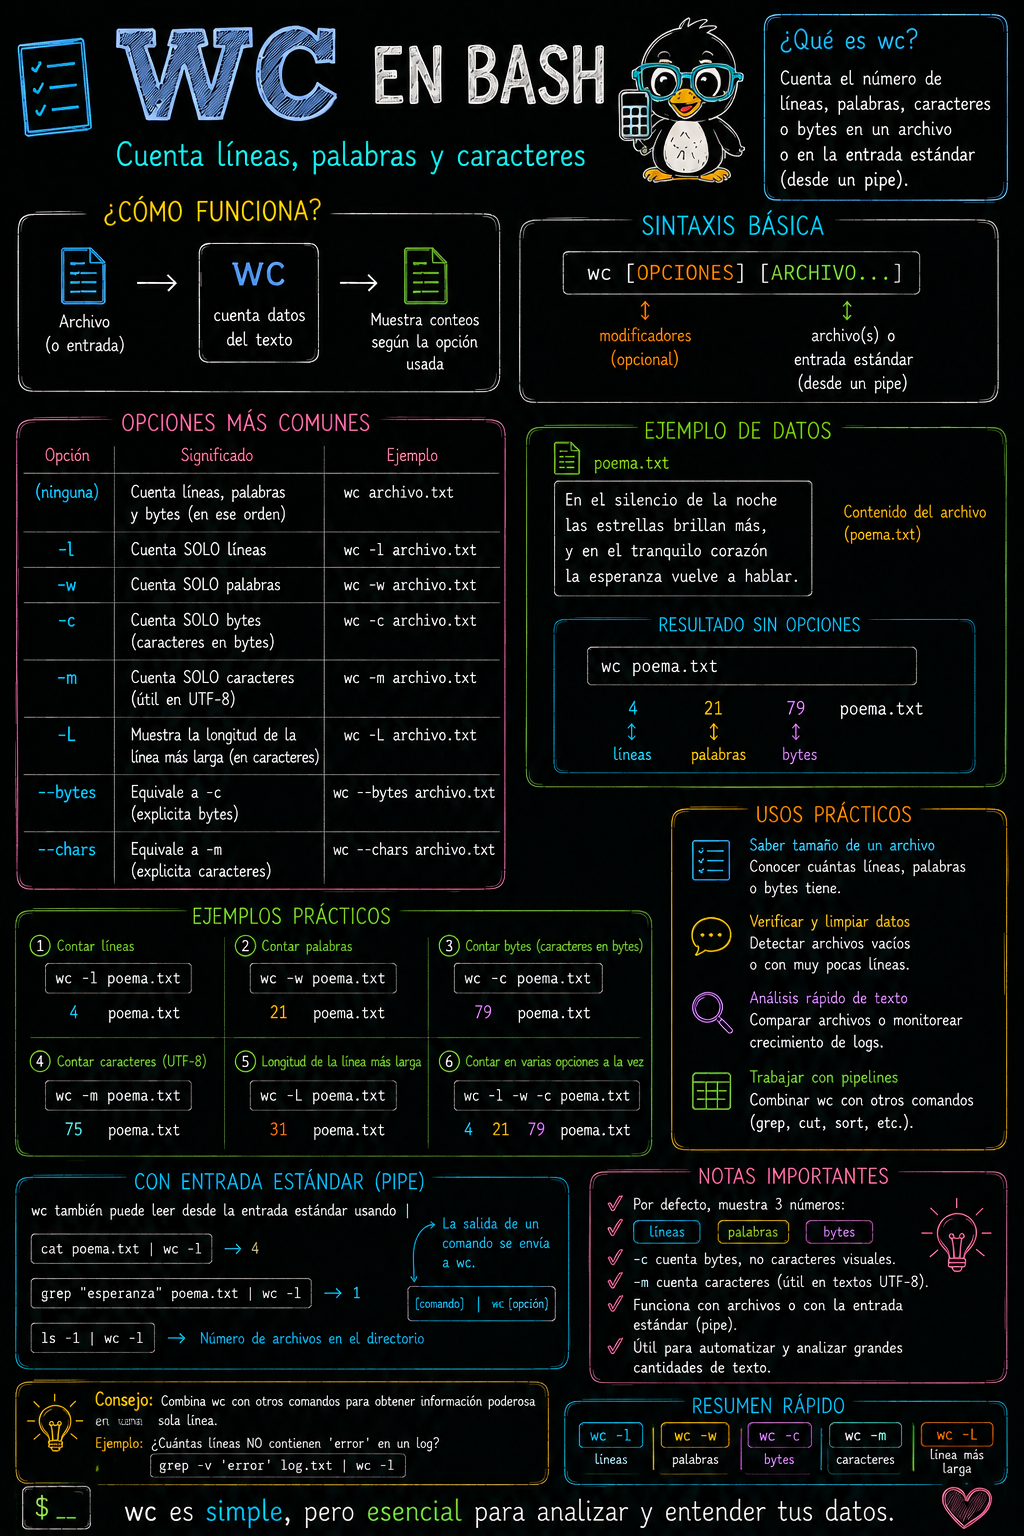
\includegraphics[keepaspectratio]{figures/bash_wc.png}}

}

\caption{Imagen creada con ChatGPT}

\end{figure}%

\section{\texorpdfstring{\texttt{cut} - Buscar patrones en
texto}{cut - Buscar patrones en texto}}\label{cut---buscar-patrones-en-texto}

Aquí vamos a partir de \textbf{¿Qué hago si no quiero toda la línea,
sino solamente una columna de un archivo?}

\textbf{Sintaxis:}

\begin{verbatim}
cut [opciones] archivo.txt
\end{verbatim}

{\def\LTcaptype{none} % do not increment counter
\begin{longtable}[]{@{}
  >{\raggedright\arraybackslash}p{(\linewidth - 4\tabcolsep) * \real{0.1290}}
  >{\raggedright\arraybackslash}p{(\linewidth - 4\tabcolsep) * \real{0.5484}}
  >{\raggedright\arraybackslash}p{(\linewidth - 4\tabcolsep) * \real{0.3118}}@{}}
\toprule\noalign{}
\begin{minipage}[b]{\linewidth}\raggedright
Argumento
\end{minipage} & \begin{minipage}[b]{\linewidth}\raggedright
Descripción
\end{minipage} & \begin{minipage}[b]{\linewidth}\raggedright
Ejemplo
\end{minipage} \\
\midrule\noalign{}
\endhead
\bottomrule\noalign{}
\endlastfoot
\texttt{-c} & Extrae caracteres por posición (ej: \texttt{-c1-5}) &
\begin{minipage}[t]{\linewidth}\raggedright
\begin{Shaded}
\begin{Highlighting}[]
\FunctionTok{cut} \AttributeTok{{-}c1{-}2}\NormalTok{ archivo.txt}
\end{Highlighting}
\end{Shaded}
\end{minipage} \\
\texttt{-f} & Extrae campos específicos (ej: \texttt{-f1,3}) &
\begin{minipage}[t]{\linewidth}\raggedright
\begin{Shaded}
\begin{Highlighting}[]
\FunctionTok{cut} \AttributeTok{{-}f1,3} \AttributeTok{{-}d:}\NormalTok{ alumnos.txt}
\end{Highlighting}
\end{Shaded}
\end{minipage} \\
\texttt{-d} & Define separador de campos (default: tabulación) &
\begin{minipage}[t]{\linewidth}\raggedright
\begin{Shaded}
\begin{Highlighting}[]
\FunctionTok{cut} \AttributeTok{{-}f2} \AttributeTok{{-}d}\StringTok{" "}\NormalTok{ datos.txt}
\end{Highlighting}
\end{Shaded}
\end{minipage} \\
\end{longtable}
}

\begin{figure}[H]

{\centering \pandocbounded{
\includegraphics[keepaspectratio]{figures/bash_cut.png}}

}

\caption{Imagen creada con ChatGPT.}

\end{figure}%

\section{\texorpdfstring{Ejercicio integrador: \texttt{grep},
\texttt{cut}, \texttt{sort}, \texttt{uniq} y
\texttt{wc}}{Ejercicio integrador: grep, cut, sort, uniq y wc}}\label{ejercicio-integrador-grep-cut-sort-uniq-y-wc}

\begin{tcolorbox}[enhanced jigsaw, arc=.35mm, bottomrule=.15mm, bottomtitle=1mm, breakable, colback=white, colbacktitle=quarto-callout-note-color!10!white, colframe=quarto-callout-note-color-frame, coltitle=black, left=2mm, leftrule=.75mm, opacityback=0, opacitybacktitle=0.6, rightrule=.15mm, title=\textcolor{quarto-callout-note-color}{\faInfo}\hspace{0.5em}{Ejercicio 10}, titlerule=0mm, toprule=.15mm, toptitle=1mm]

Instrucciones

\begin{enumerate}
\def\labelenumi{\arabic{enumi}.}
\item
  Crea el archivo \texttt{materias.txt} ejercutando el siguiente
  comando:

\begin{Shaded}
\begin{Highlighting}[]
\BuiltInTok{echo} \AttributeTok{{-}e} \StringTok{"Álgebra Lineal:8:1\textbackslash{}nCálculo Diferencial:10:1\textbackslash{}nGeometría Analítica:8:1\textbackslash{}nProbabilidad:6:3\textbackslash{}nEstadística:6:3\textbackslash{}nEcuaciones Diferenciales:8:4\textbackslash{}nÁlgebra Abstracta:8:5\textbackslash{}nTopología:6:6\textbackslash{}nAnálisis Real:8:6\textbackslash{}nProbabilidad:6:3"} \OperatorTok{\textgreater{}}\NormalTok{ ejercicios/BASH/materias.txt}
\end{Highlighting}
\end{Shaded}

  \textbf{Columna 1:} materias, \textbf{Columna 2:} créditos,
  \textbf{Columna 3:} semestre.
\item
  Mostrar todas las materias que contienen la palabra Álgebra.
\item
  Mostrar todas las materias de sexto semestre.
\item
  Contar cuántas materias tienen 8 créditos.
\item
  Mostrar únicamente los nombres de las materias.
\item
  Mostrar únicamente los créditos.
\item
  Ordenar las materias alfabéticamente.
\item
  Ordenar los créditos de menor a mayor.
\item
  Mostrar los semestres sin repetir.
\item
  Contar cuántas materias hay por semestre.
\item
  ¿Cuántas materias hay por número de créditos?
\item
  ¿Cuál es el número de créditos más frecuente?
\end{enumerate}

\begin{quote}
\textbf{Solucion}

\begin{Shaded}
\begin{Highlighting}[]
\ExtensionTok{2.}\NormalTok{ grep }\StringTok{"Álgebra"}\NormalTok{ ejercicios/BASH/materias.txt}
\ExtensionTok{3.}\NormalTok{ grep }\StringTok{":6$"}\NormalTok{ ejercicios/BASH/materias.txt}
\ExtensionTok{4.}\NormalTok{ grep }\StringTok{":8:"}\NormalTok{ ejercicios/BASH/materias.txt }\KeywordTok{|} \FunctionTok{wc} \AttributeTok{{-}l}
\ExtensionTok{5.}\NormalTok{ cut }\AttributeTok{{-}d}\StringTok{":"} \AttributeTok{{-}f1}\NormalTok{ ejercicios/BASH/materias.txt}
\ExtensionTok{6.}\NormalTok{ cut }\AttributeTok{{-}d}\StringTok{":"} \AttributeTok{{-}f2}\NormalTok{ ejercicios/BASH/materias.txt}
\ExtensionTok{7.}\NormalTok{ cut }\AttributeTok{{-}d}\StringTok{":"} \AttributeTok{{-}f1}\NormalTok{ ejercicios/BASH/materias.txt }\KeywordTok{|} \FunctionTok{sort}
\ExtensionTok{8.}\NormalTok{ cut }\AttributeTok{{-}d}\StringTok{":"} \AttributeTok{{-}f2}\NormalTok{ ejercicios/BASH/materias.txt }\KeywordTok{|} \FunctionTok{sort} \AttributeTok{{-}n}
\ExtensionTok{9.}\NormalTok{ cut }\AttributeTok{{-}d}\StringTok{":"} \AttributeTok{{-}f3}\NormalTok{ ejercicios/BASH/materias.txt }\KeywordTok{|} \FunctionTok{sort} \KeywordTok{|} \FunctionTok{uniq}
\ExtensionTok{10.}\NormalTok{ cut }\AttributeTok{{-}d}\StringTok{":"} \AttributeTok{{-}f3}\NormalTok{ ejercicios/BASH/materias.txt }\KeywordTok{|} \FunctionTok{sort} \KeywordTok{|} \FunctionTok{uniq} \AttributeTok{{-}c}
\ExtensionTok{11.}\NormalTok{ cut }\AttributeTok{{-}d}\StringTok{":"} \AttributeTok{{-}f2}\NormalTok{ ejercicios/BASH/materias.txt }\KeywordTok{|} \FunctionTok{sort} \KeywordTok{|} \FunctionTok{uniq} \AttributeTok{{-}c}
\ExtensionTok{12.}\NormalTok{ cut }\AttributeTok{{-}d}\StringTok{":"} \AttributeTok{{-}f2}\NormalTok{ ejercicios/BASH/materias.txt }\KeywordTok{|} \FunctionTok{sort} \KeywordTok{|} \FunctionTok{uniq} \AttributeTok{{-}c} \KeywordTok{|} \FunctionTok{sort} \AttributeTok{{-}nr} \KeywordTok{|} \FunctionTok{head} \AttributeTok{{-}1}
\end{Highlighting}
\end{Shaded}
\end{quote}

\end{tcolorbox}

\section{Referencias}\label{referencias-8}

\begin{itemize}
\tightlist
\item
  \href{https://vinuesa.github.io/intro2linux/index.html\#ejemplos-de-herramientas-de-filtrado-de-texto-pipelines-con-grep-cut-sort-uniq-wc-en-acci\%C3\%B3n}{Ejemplos
  de herramientas de filtrado de texto: \emph{pipelines} con
  \textbf{grep}, \textbf{cut}, \textbf{sort}, \textbf{uniq}, \textbf{wc}
  en acción}
\end{itemize}

\chapter{Scripts en Bash}\label{scripts-en-bash}

\begin{quote}
\textbf{Fecha:} 29 de septiembre, 2026
\end{quote}

\section{¿Qué es un script de Bash?}\label{quuxe9-es-un-script-de-bash}

Los \texttt{scripts} son archivos de texto que contienen instrucciones
ejecutables por un intérprete de un lenguaje de programación para la
ejecución de tareas. El formato \texttt{.sh} se utiliza para escribir
\texttt{scripts\ ejecutables} por un intérprete como \textbf{Bash}.

En esta sección crearemos varios scripts de Bash y usaremos varios
comandos y operadores.

\begin{tcolorbox}[enhanced jigsaw, arc=.35mm, bottomrule=.15mm, bottomtitle=1mm, breakable, colback=white, colbacktitle=quarto-callout-note-color!10!white, colframe=quarto-callout-note-color-frame, coltitle=black, left=2mm, leftrule=.75mm, opacityback=0, opacitybacktitle=0.6, rightrule=.15mm, title={Estructura básica de un script}, titlerule=0mm, toprule=.15mm, toptitle=1mm]

Los script de Bash contiene al inicio esta descripción
\texttt{\#!bin/bash} y la extensión \texttt{.sh}

\begin{Shaded}
\begin{Highlighting}[]
\CommentTok{\#!/bin/bash}
\CommentTok{\# Comentario: esto es un script básico}

\BuiltInTok{echo} \StringTok{"Hola, mundo"}
\end{Highlighting}
\end{Shaded}

\end{tcolorbox}

\subsection{Componentes clave}\label{componentes-clave}

\textbf{Shebang (\texttt{\#!/bin/bash})}

\begin{itemize}
\tightlist
\item
  Primera línea del script
\item
  Indica al sistema que use Bash para ejecutar el archivo
\item
  Debe estar en la primera línea, sin espacios antes
\end{itemize}

\textbf{Comentarios (\texttt{\#})}

\begin{itemize}
\tightlist
\item
  Líneas que comienzan con \texttt{\#} son ignoradas
\item
  Útiles para documentar el código
\end{itemize}

\textbf{Comandos}

\begin{itemize}
\tightlist
\item
  Instrucciones que se ejecutan línea por línea
\end{itemize}

\subsection{Crear y ejecutar un
script}\label{crear-y-ejecutar-un-script}

\begin{verbatim}
# 1. Crear el archivo
nano mi_script.sh

# 2. Hacer el archivo ejecutable
chmod +x mi_script.sh

# 3. Ejecutar el script
./mi_script.sh

# O ejecutar sin permisos de ejecución
bash mi_script.sh
\end{verbatim}

\begin{figure}[H]

{\centering \pandocbounded{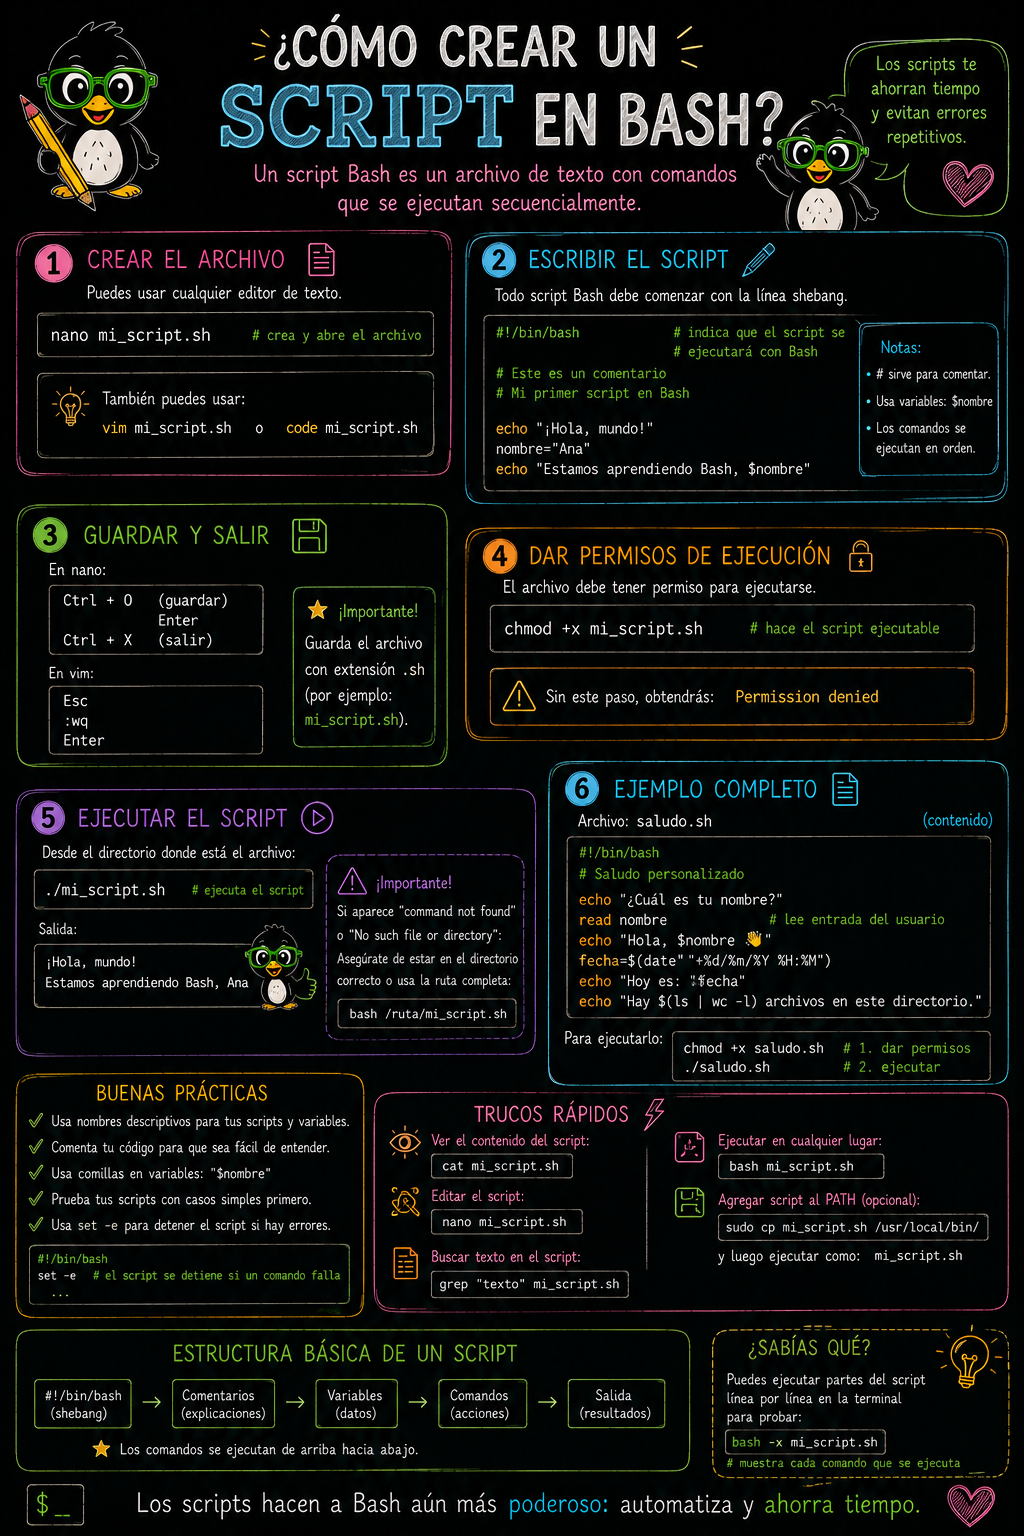
\includegraphics[keepaspectratio]{figures/bash_script_overview.png}}

}

\caption{Imagen creada con ChatGPT.}

\end{figure}%

\section{Variables en Bash}\label{variables-en-bash}

\subsection{¿Qué es una variable?}\label{quuxe9-es-una-variable}

Un contenedor que almacena un valor (texto, números, etc.) que puede
cambiar durante la ejecución del script.

\subsection{Declaración y
asignación}\label{declaraciuxf3n-y-asignaciuxf3n}

\begin{Shaded}
\begin{Highlighting}[]
\VariableTok{nombre}\OperatorTok{=}\StringTok{"Juan"}
\VariableTok{edad}\OperatorTok{=}\NormalTok{25}
\VariableTok{ciudad}\OperatorTok{=}\StringTok{"Madrid"}
\end{Highlighting}
\end{Shaded}

\textbf{Reglas importantes:}

\begin{itemize}
\tightlist
\item
  ✅ Sin espacios alrededor del \texttt{=}
\item
  ✅ Nombres en minúsculas (por convención)
\item
  ✅ Pueden contener letras, números y guiones bajos
\item
  ❌ No pueden comenzar con números
\end{itemize}

\subsection{Acceder a variables}\label{acceder-a-variables}

\begin{Shaded}
\begin{Highlighting}[]
\BuiltInTok{echo} \VariableTok{$nombre}           \CommentTok{\# Imprime el valor}
\BuiltInTok{echo} \VariableTok{$\{nombre\}}         \CommentTok{\# Forma alternativa (más segura)}
\BuiltInTok{echo} \StringTok{"Hola, }\VariableTok{$nombre}\StringTok{"}   \CommentTok{\# Dentro de comillas dobles}
\end{Highlighting}
\end{Shaded}

\subsection{Tipos de variables}\label{tipos-de-variables}

\subsubsection{Variables de cadena
(string)}\label{variables-de-cadena-string}

\begin{Shaded}
\begin{Highlighting}[]
\VariableTok{nombre}\OperatorTok{=}\StringTok{"María"}
\VariableTok{mensaje}\OperatorTok{=}\StringTok{"Bienvenido a Bash"}
\end{Highlighting}
\end{Shaded}

\subsubsection{Variables numéricas}\label{variables-numuxe9ricas}

\begin{Shaded}
\begin{Highlighting}[]
\VariableTok{edad}\OperatorTok{=}\NormalTok{30}
\VariableTok{cantidad}\OperatorTok{=}\NormalTok{100}
\end{Highlighting}
\end{Shaded}

\subsubsection{Variables vacías}\label{variables-vacuxedas}

\begin{Shaded}
\begin{Highlighting}[]
\VariableTok{variable}\OperatorTok{=}\StringTok{""}
\end{Highlighting}
\end{Shaded}

\subsection{Comillas simples
vs.~dobles}\label{comillas-simples-vs.-dobles}

\begin{Shaded}
\begin{Highlighting}[]
\VariableTok{nombre}\OperatorTok{=}\StringTok{"Juan"}
\BuiltInTok{echo} \StringTok{"Hola, }\VariableTok{$nombre}\StringTok{"}      \CommentTok{\# Hola, Juan (interpreta variables)}
\BuiltInTok{echo} \StringTok{\textquotesingle{}Hola, $nombre\textquotesingle{}}      \CommentTok{\# Hola, $nombre (literal)}
\end{Highlighting}
\end{Shaded}

\subsection{Variables especiales}\label{variables-especiales}

\begin{Shaded}
\begin{Highlighting}[]
\VariableTok{$0}      \CommentTok{\# Nombre del script}
\VariableTok{$1}\ExtensionTok{,} \VariableTok{$2}  \CommentTok{\# Argumentos pasados al script}
\VariableTok{$\#}      \CommentTok{\# Número de argumentos}
\VariableTok{$?}      \CommentTok{\# Código de salida del último comando}
\VariableTok{$$}      \CommentTok{\# ID del proceso actual}
\end{Highlighting}
\end{Shaded}

\begin{figure}[H]

{\centering \pandocbounded{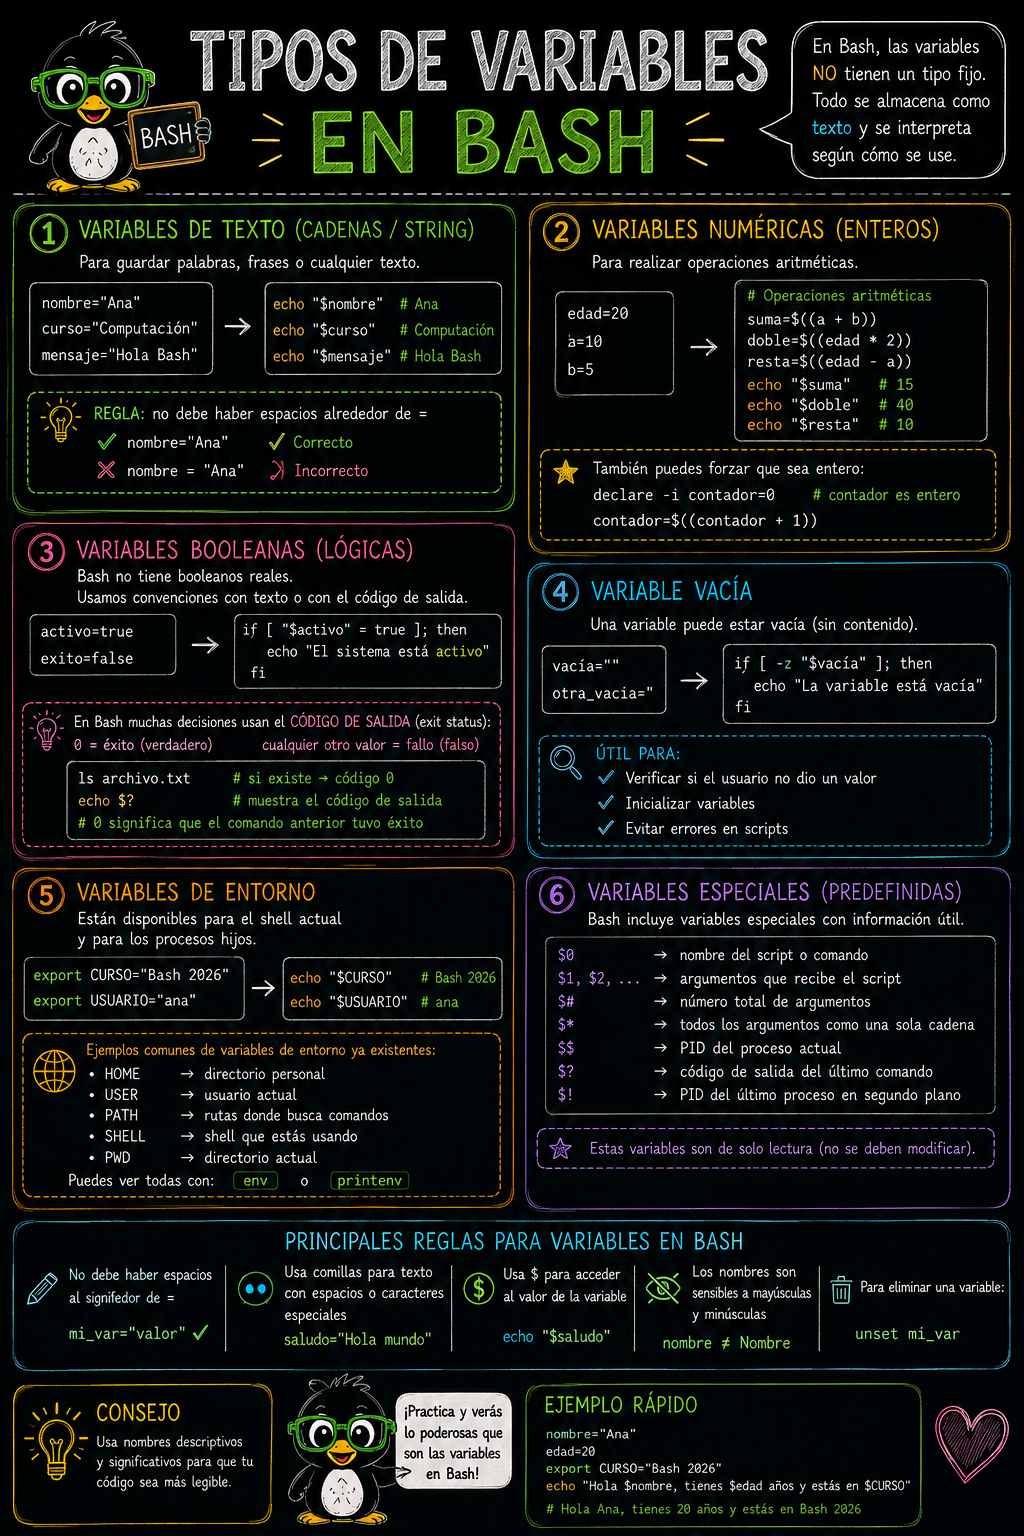
\includegraphics[keepaspectratio]{figures/bash_variables.png}}

}

\caption{Imagen creada con ChatGPT.}

\end{figure}%

\section{\texorpdfstring{\textbf{Nivel 1: Scripts
básicos}}{Nivel 1: Scripts básicos}}\label{nivel-1-scripts-buxe1sicos}

\subsection{Primer script}\label{primer-script}

Archivo: \texttt{saludo.sh}

\begin{Shaded}
\begin{Highlighting}[]
\CommentTok{\#!/bin/bash}

\BuiltInTok{echo} \StringTok{"¡Bienvenido a Bash!"}
\BuiltInTok{echo} \StringTok{"Este es mi primer script"}
\end{Highlighting}
\end{Shaded}

Ejecución:

\begin{Shaded}
\begin{Highlighting}[]
\FunctionTok{chmod}\NormalTok{ +x saludo.sh}
\ExtensionTok{./saludo.sh}
\end{Highlighting}
\end{Shaded}

Esperando una salida como esta:

\begin{verbatim}
¡Bienvenido a Bash!
Este es mi primer script
\end{verbatim}

\subsection{Script con variables
simples}\label{script-con-variables-simples}

Archivo: \texttt{presentacion.sh}

\begin{Shaded}
\begin{Highlighting}[]
\CommentTok{\#!/bin/bash}

\VariableTok{nombre}\OperatorTok{=}\StringTok{"Carlos"}
\VariableTok{edad}\OperatorTok{=}\NormalTok{28}
\VariableTok{ciudad}\OperatorTok{=}\StringTok{"Barcelona"}

\BuiltInTok{echo} \StringTok{"Mi nombre es }\VariableTok{$nombre}\StringTok{"}
\BuiltInTok{echo} \StringTok{"Tengo }\VariableTok{$edad}\StringTok{ años"}
\BuiltInTok{echo} \StringTok{"Vivo en }\VariableTok{$ciudad}\StringTok{"}
\end{Highlighting}
\end{Shaded}

Ejecución:

\begin{Shaded}
\begin{Highlighting}[]
\FunctionTok{chmod}\NormalTok{ +x presentacion.sh}
\ExtensionTok{./presentacion.sh}
\end{Highlighting}
\end{Shaded}

Esperando una salida como esta:

\begin{verbatim}
Mi nombre es Carlos
Tengo 28 años
Vivo en Barcelona
\end{verbatim}

\subsection{Concatenación de
variables}\label{concatenaciuxf3n-de-variables}

Archivo: \texttt{concatenar.sh}

\begin{Shaded}
\begin{Highlighting}[]
\CommentTok{\#!/bin/bash}

\VariableTok{nombre}\OperatorTok{=}\StringTok{"Evelia"}
\VariableTok{apellido}\OperatorTok{=}\StringTok{"Coss"}
\VariableTok{edad}\OperatorTok{=}\NormalTok{32}

\BuiltInTok{echo} \StringTok{"Nombre completo: }\VariableTok{$nombre}\StringTok{ }\VariableTok{$apellido}\StringTok{"}
\BuiltInTok{echo} \StringTok{"Información: }\VariableTok{$nombre}\StringTok{ tiene }\VariableTok{$edad}\StringTok{ años"}
\end{Highlighting}
\end{Shaded}

Ejecución:

\begin{Shaded}
\begin{Highlighting}[]
\FunctionTok{chmod}\NormalTok{ +x concatenar.sh}
\ExtensionTok{./concatenar.sh}
\end{Highlighting}
\end{Shaded}

Esperando una salida como esta:

\begin{verbatim}
Nombre completo: Evelia Coss
Información: Evelia tiene 32 años
\end{verbatim}

\section{\texorpdfstring{\textbf{Nivel 2: Entrada de
datos}}{Nivel 2: Entrada de datos}}\label{nivel-2-entrada-de-datos}

\subsection{Leer entrada del usuario}\label{leer-entrada-del-usuario}

Archivo: \texttt{leer\_entrada.sh}

\begin{Shaded}
\begin{Highlighting}[]
\CommentTok{\#!/bin/bash}

\BuiltInTok{echo} \StringTok{"¿Cuál es tu nombre?"}
\BuiltInTok{read} \VariableTok{nombre}

\BuiltInTok{echo} \StringTok{"¿Cuál es tu edad?"}
\BuiltInTok{read} \VariableTok{edad}

\BuiltInTok{echo} \StringTok{"Hola }\VariableTok{$nombre}\StringTok{, tienes }\VariableTok{$edad}\StringTok{ años"}
\end{Highlighting}
\end{Shaded}

Ejecución:

\begin{Shaded}
\begin{Highlighting}[]
\FunctionTok{chmod}\NormalTok{ +x leer\_entrada.sh}
\ExtensionTok{./leer\_entrada.sh}
\end{Highlighting}
\end{Shaded}

Esperando una salida como esta:

\begin{verbatim}
¿Cuál es tu nombre? # Te va a preguntar 
Evelia
¿Cuál es tu edad?  # Te va a preguntar 
32
Hola Evelia, tienes 32 años
\end{verbatim}

\subsection{\texorpdfstring{Múltiples variables con
\texttt{read}}{Múltiples variables con read}}\label{muxfaltiples-variables-con-read}

Archivo: \texttt{datos\_personales.sh}

\begin{Shaded}
\begin{Highlighting}[]
\CommentTok{\#!/bin/bash}

\BuiltInTok{echo} \StringTok{"Ingresa tu nombre, edad y ciudad (separados por espacio):"}
\BuiltInTok{read} \VariableTok{nombre} \VariableTok{edad} \VariableTok{ciudad}

\BuiltInTok{echo} \StringTok{"Datos ingresados:"}
\BuiltInTok{echo} \StringTok{"Nombre: }\VariableTok{$nombre}\StringTok{"}
\BuiltInTok{echo} \StringTok{"Edad: }\VariableTok{$edad}\StringTok{"}
\BuiltInTok{echo} \StringTok{"Ciudad: }\VariableTok{$ciudad}\StringTok{"}
\end{Highlighting}
\end{Shaded}

Ejecución:

\begin{Shaded}
\begin{Highlighting}[]
\FunctionTok{chmod}\NormalTok{ +x datos\_personales.sh}
\ExtensionTok{./datos\_personales.sh}
\end{Highlighting}
\end{Shaded}

Esperando una salida como esta:

\begin{verbatim}
Ingresa tu nombre, edad y ciudad (separados por espacio):
Evelia 32 Queretaro
Datos ingresados:
Nombre: Evelia
Edad: 32
Ciudad: Queretaro
\end{verbatim}

\subsection{Leer con mensaje
personalizado}\label{leer-con-mensaje-personalizado}

Archivo: \texttt{leer\_con\_prompt.sh}

\begin{Shaded}
\begin{Highlighting}[]
\CommentTok{\#!/bin/bash}

\BuiltInTok{read} \AttributeTok{{-}p} \StringTok{"¿Cuál es tu nombre? "} \VariableTok{nombre}
\BuiltInTok{read} \AttributeTok{{-}p} \StringTok{"¿Cuál es tu email? "} \VariableTok{email}

\BuiltInTok{echo} \StringTok{"Nombre: }\VariableTok{$nombre}\StringTok{"}
\BuiltInTok{echo} \StringTok{"Email: }\VariableTok{$email}\StringTok{"}
\end{Highlighting}
\end{Shaded}

Ejecución:

\begin{Shaded}
\begin{Highlighting}[]
\FunctionTok{chmod}\NormalTok{ +x leer\_con\_prompt.sh}
\ExtensionTok{./leer\_con\_prompt.sh}
\end{Highlighting}
\end{Shaded}

Esperando una salida como esta:

\begin{verbatim}
¿Cuál es tu nombre? Evelia
¿Cuál es tu email? ecossnav@gmail.com
Nombre: Evelia
Email: ecossnav@gmail.com
\end{verbatim}

\section{\texorpdfstring{\textbf{Nivel 3: Argumentos del
script}}{Nivel 3: Argumentos del script}}\label{nivel-3-argumentos-del-script}

\subsection{Usar argumentos}\label{usar-argumentos}

Archivo: \texttt{argumentos.sh}

\begin{Shaded}
\begin{Highlighting}[]
\CommentTok{\#!/bin/bash}

\BuiltInTok{echo} \StringTok{"Primer argumento: }\VariableTok{$1}\StringTok{"}
\BuiltInTok{echo} \StringTok{"Segundo argumento: }\VariableTok{$2}\StringTok{"}
\BuiltInTok{echo} \StringTok{"Tercer argumento: }\VariableTok{$3}\StringTok{"}
\BuiltInTok{echo} \StringTok{"Total de argumentos: }\VariableTok{$\#}\StringTok{"}
\end{Highlighting}
\end{Shaded}

Ejecución:

\begin{Shaded}
\begin{Highlighting}[]
\FunctionTok{chmod}\NormalTok{ +x argumentos.sh}
\ExtensionTok{./argumentos.sh}\NormalTok{ Juan 25 Madrid}
\end{Highlighting}
\end{Shaded}

Esperando una salida como esta:

\begin{verbatim}
Primer argumento: Juan
Segundo argumento: 25
Tercer argumento: Madrid
Total de argumentos: 3
\end{verbatim}

\subsection{Script con argumentos
obligatorios}\label{script-con-argumentos-obligatorios}

\begin{tcolorbox}[enhanced jigsaw, arc=.35mm, bottomrule=.15mm, bottomtitle=1mm, breakable, colback=white, colbacktitle=quarto-callout-important-color!10!white, colframe=quarto-callout-important-color-frame, coltitle=black, left=2mm, leftrule=.75mm, opacityback=0, opacitybacktitle=0.6, rightrule=.15mm, title={Importante}, titlerule=0mm, toprule=.15mm, toptitle=1mm]

\textbf{Dobles paréntesis \texttt{((\ ))}} indican que lo que está
dentro es una expresión aritmética.

\end{tcolorbox}

Archivo: \texttt{sumar\_argumentos.sh}

\begin{Shaded}
\begin{Highlighting}[]
\CommentTok{\#!/bin/bash}

\VariableTok{num1}\OperatorTok{=}\VariableTok{$1}
\VariableTok{num2}\OperatorTok{=}\VariableTok{$2}

\VariableTok{suma}\OperatorTok{=}\VariableTok{$((num1} \OperatorTok{+} \VariableTok{num2))}

\BuiltInTok{echo} \StringTok{"}\VariableTok{$num1}\StringTok{ + }\VariableTok{$num2}\StringTok{ = }\VariableTok{$suma}\StringTok{"}
\end{Highlighting}
\end{Shaded}

Ejecución:

\begin{Shaded}
\begin{Highlighting}[]
\FunctionTok{chmod}\NormalTok{ +x sumar\_argumentos.sh}
\ExtensionTok{./sumar\_argumentos.sh}\NormalTok{ 10 20}
\end{Highlighting}
\end{Shaded}

Esperando una salida como esta:

\begin{verbatim}
10 + 20 = 30
\end{verbatim}

\section{Nivel 4: Operaciones con
variables}\label{nivel-4-operaciones-con-variables}

\subsection{Operaciones aritméticas}\label{operaciones-aritmuxe9ticas}

Archivo: \texttt{operaciones.sh}

\begin{Shaded}
\begin{Highlighting}[]
\CommentTok{\#!/bin/bash}

\VariableTok{a}\OperatorTok{=}\NormalTok{10}
\VariableTok{b}\OperatorTok{=}\NormalTok{5}

\VariableTok{suma}\OperatorTok{=}\VariableTok{$((a} \OperatorTok{+} \VariableTok{b))}
\VariableTok{resta}\OperatorTok{=}\VariableTok{$((a} \OperatorTok{{-}} \VariableTok{b))}
\VariableTok{multiplicacion}\OperatorTok{=}\VariableTok{$((a} \OperatorTok{*} \VariableTok{b))}
\VariableTok{division}\OperatorTok{=}\VariableTok{$((a} \OperatorTok{/} \VariableTok{b))}

\BuiltInTok{echo} \StringTok{"Suma: }\VariableTok{$suma}\StringTok{"}
\BuiltInTok{echo} \StringTok{"Resta: }\VariableTok{$resta}\StringTok{"}
\BuiltInTok{echo} \StringTok{"Multiplicación: }\VariableTok{$multiplicacion}\StringTok{"}
\BuiltInTok{echo} \StringTok{"División: }\VariableTok{$division}\StringTok{"}
\end{Highlighting}
\end{Shaded}

Ejecución:

\begin{Shaded}
\begin{Highlighting}[]
\FunctionTok{chmod}\NormalTok{ +x operaciones.sh}
\ExtensionTok{./operaciones.sh}
\end{Highlighting}
\end{Shaded}

Esperando una salida como esta:

\begin{verbatim}
Suma: 15
Resta: 5
Multiplicación: 50
División: 2
\end{verbatim}

\subsection{Incremento y decremento}\label{incremento-y-decremento}

Archivo: \texttt{incremento.sh}

\begin{Shaded}
\begin{Highlighting}[]
\CommentTok{\#!/bin/bash}

\VariableTok{contador}\OperatorTok{=}\NormalTok{0}

\BuiltInTok{echo} \StringTok{"Contador inicial: }\VariableTok{$contador}\StringTok{"}

\VariableTok{contador}\OperatorTok{=}\VariableTok{$((contador} \OperatorTok{+} \DecValTok{1}\VariableTok{))}
\BuiltInTok{echo} \StringTok{"Después de incrementar: }\VariableTok{$contador}\StringTok{"}

\VariableTok{contador}\OperatorTok{=}\VariableTok{$((contador} \OperatorTok{{-}} \DecValTok{1}\VariableTok{))}
\BuiltInTok{echo} \StringTok{"Después de decrementar: }\VariableTok{$contador}\StringTok{"}
\end{Highlighting}
\end{Shaded}

Ejecución:

\begin{Shaded}
\begin{Highlighting}[]
\FunctionTok{chmod}\NormalTok{ +x incremento.sh}
\ExtensionTok{./incremento.sh}
\end{Highlighting}
\end{Shaded}

Esperando una salida como esta:

\begin{verbatim}
Después de incrementar: 1
Después de decrementar: 0
\end{verbatim}

\subsection{Longitud de una cadena}\label{longitud-de-una-cadena}

Archivo: \texttt{longitud.sh}

\begin{Shaded}
\begin{Highlighting}[]
\CommentTok{\#!/bin/bash}

\VariableTok{texto}\OperatorTok{=}\StringTok{"Hola Bash"}
\VariableTok{longitud}\OperatorTok{=}\VariableTok{$\{}\OperatorTok{\#}\VariableTok{texto\}} \CommentTok{\# obtener la cantidad de caracteres que tiene una variable}

\BuiltInTok{echo} \StringTok{"Texto: }\VariableTok{$texto}\StringTok{"}
\BuiltInTok{echo} \StringTok{"Longitud: }\VariableTok{$longitud}\StringTok{ caracteres"}
\end{Highlighting}
\end{Shaded}

Ejecución:

\begin{Shaded}
\begin{Highlighting}[]
\FunctionTok{chmod}\NormalTok{ +x longitud.sh}
\ExtensionTok{./longitud.sh}
\end{Highlighting}
\end{Shaded}

Esperando una salida como esta:

\begin{verbatim}
Texto: Hola Bash
Longitud: 9 caracteres
\end{verbatim}

\section{Nivel 5. Variables de
entorno}\label{nivel-5.-variables-de-entorno}

\subsection{Usar variables de entorno}\label{usar-variables-de-entorno}

Archivo: \texttt{variables\_entorno.sh}

\begin{Shaded}
\begin{Highlighting}[]
\CommentTok{\#!/bin/bash}

\BuiltInTok{echo} \StringTok{"Usuario actual: }\VariableTok{$USER}\StringTok{"}
\BuiltInTok{echo} \StringTok{"Directorio home: }\VariableTok{$HOME}\StringTok{"}
\BuiltInTok{echo} \StringTok{"Directorio actual: }\VariableTok{$PWD}\StringTok{"}
\BuiltInTok{echo} \StringTok{"Sistema operativo: }\VariableTok{$OSTYPE}\StringTok{"}
\end{Highlighting}
\end{Shaded}

Ejecución:

\begin{Shaded}
\begin{Highlighting}[]
\FunctionTok{chmod}\NormalTok{ +x variables\_entorno.sh}
\ExtensionTok{./variables\_entorno.sh}
\end{Highlighting}
\end{Shaded}

Esperando una salida como esta:

\begin{verbatim}
Usuario actual: ecoss
Directorio home: /Users/ecoss
Directorio actual: /Users/ecoss/Documents/Mt_TallerComputo_ClaseBash
Sistema operativo: darwin25
\end{verbatim}

\subsection{Crear y usar variables de
entorno}\label{crear-y-usar-variables-de-entorno}

Archivo: \texttt{crear\_entorno.sh}

\begin{Shaded}
\begin{Highlighting}[]
\CommentTok{\#!/bin/bash}

\BuiltInTok{export} \VariableTok{MI\_VARIABLE}\OperatorTok{=}\StringTok{"Valor importante"}

\BuiltInTok{echo} \StringTok{"Mi variable: }\VariableTok{$MI\_VARIABLE}\StringTok{"}
\end{Highlighting}
\end{Shaded}

Ejecución:

\begin{Shaded}
\begin{Highlighting}[]
\FunctionTok{chmod}\NormalTok{ +x crear\_entorno.sh}
\ExtensionTok{./crear\_entorno.sh}
\end{Highlighting}
\end{Shaded}

Esperando una salida como esta:

\begin{verbatim}
Mi variable: Valor importante
\end{verbatim}

\section{Material suplementario}\label{material-suplementario-5}

\begin{itemize}
\tightlist
\item
  RSG Ecuador.
  \href{https://rsg-ecuador.github.io/unix.bioinfo.rsgecuador/content/Curso_avanzado/02_Bash/1_bash.html}{Scripts
  en Bash}
\item
  RSG Ecuador.
  \href{https://rsg-ecuador.github.io/unix.bioinfo.rsgecuador/content/Curso_basico/03_Manejo_terminal/5_wildcards.html}{Wildcards
  y Streams}
\item
  RSG Ecuador.
  \href{https://rsg-ecuador.github.io/unix.bioinfo.rsgecuador/content/Curso_basico/04_Procesamiento_ficheros_regex_pipes/3_Expresiones_regulares.html}{Expresiones
  regulares (\emph{regex})}
\item
  \href{https://pressbooks.senecapolytechnic.ca/uli101/chapter/wildcard-selection-in-bash/}{Wildcard
  Selection in Bash}
\end{itemize}

\chapter{\texorpdfstring{\textbf{📚 Actividad 2 en equipo -} Script
Bash}{📚 Actividad 2 en equipo - Script Bash}}\label{actividad-2-en-equipo---script-bash}

\begin{quote}
\textbf{Fecha de entrega:} Martes 01 de octubre, 2026 a las 11:59 pm.
\end{quote}

\section{Instrucciones}\label{instrucciones}

En equipos de \textbf{2 a 3} \textbf{personas}, seleccionar uno de los
siguientes temas y realizar un proyecto aplicando \textbf{buenas
prácticas de programación}. El proceso debe estar completamente
documentado y entregarse en \textbf{Google Classroom:}

\begin{enumerate}
\def\labelenumi{\arabic{enumi}.}
\tightlist
\item
  Carpeta a entregar comprimida (\texttt{.zip}).
\item
  \textbf{Documentación del proyecto:} Documento explicativo del
  desarrollo del programa en Google docs. Agregar en la tarea \emph{solo
  el link del documento}.
\item
  Subir en Youtube un video de aproximadamente 5 minutos describiendo el
  proceso y resultados. Agregar en la tarea \emph{solo el link del
  video}.
\end{enumerate}

\subsection{Estructura de la carpeta a
entregar}\label{estructura-de-la-carpeta-a-entregar}

\begin{verbatim}
Proyecto_[NombreEquipo]_[NombreProyecto].zip
│
├── script.sh                          # Script principal
├── datos_entrada.txt                  # Archivo de datos (txt, csv o tsv)
├── salida_procesada.txt               # Resultado de ejecutar el script
\end{verbatim}

\subsection{ARCHIVO: script.sh 🔧}\label{archivo-script.sh}

Checklist de buenas prácticas:

\begin{itemize}
\tightlist
\item[$\square$]
  Nombre descriptivo para el script.
\item[$\square$]
  Shebang en la primera línea (\texttt{\#!/bin/bash})
\item[$\square$]
  Encabezado con información del script (nombre, descripción, autor,
  fecha)
\item[$\square$]
  Comentarios explicativos en cada sección.
\item[$\square$]
  Variables bien nombradas (descriptivas)
\item[$\square$]
  Validación de argumentos
\item[$\square$]
  Validación de archivos
\item[$\square$]
  Código indentado y organizado
\end{itemize}

\begin{verbatim}
#!/bin/bash

################################################################################
# NOMBRE DEL SCRIPT: Título
# DESCRIPCIÓN: Procesa un archivo de calificaciones y genera reportes
# AUTORES: Nombre de los estudiantes
# FECHA: Día/Mes/Año
# VERSIÓN: 1.0
# USO: ./script.sh archivo_entrada.txt
# ARGUMENTOS (opcional)
################################################################################
\end{verbatim}

\subsection{ARCHIVO: datos\_entrada.txt (o .csv, .tsv)
📊}\label{archivo-datos_entrada.txt-o-.csv-.tsv}

Requisitos:

\begin{itemize}
\tightlist
\item[$\square$]
  Mínimo 10 registros
\item[$\square$]
  Datos realistas y variados
\item[$\square$]
  Encabezado descriptivo (si aplica)
\item[$\square$]
  Nombre descriptivo del archivo
\end{itemize}

\subsection{ARCHIVO: salida\_procesada.txt
📤}\label{archivo-salida_procesada.txt}

Requisitos:

\begin{itemize}
\tightlist
\item[$\square$]
  Generado automáticamente por el script
\item[$\square$]
  Contiene toda la salida del programa
\item[$\square$]
  Formato legible y organizado
\item[$\square$]
  Incluye encabezados y separadores
\end{itemize}

\subsection{Documentación del
proyecto}\label{documentaciuxf3n-del-proyecto}

Requisitos:

\begin{itemize}
\tightlist
\item[$\square$]
  Información general: Título del proyecto, Nombre de los integrantes
  del equipo, Fecha de entrega, Versión del script: 1.0.
\item[$\square$]
  Descripción del proyecto (200 palabras máximo)
\item
  {[} {]}
\end{itemize}

\chapter{Condicionales}\label{condicionales}

\begin{quote}
\textbf{Fecha:} 01 de octubre, 2026
\end{quote}

\textbf{Objetivos:}

\begin{itemize}
\item
  \textbf{Comprender la lógica de condicionales} → Identificar cuándo y
  cómo aplicar \texttt{if}, \texttt{else} y \texttt{elif} para tomar
  decisiones en un script.
\item
  \textbf{Aplicar condicionales en scripts} → Resolver problemas
  prácticos mediante condiciones (ej. verificar existencia de archivos,
  validar entradas).
\end{itemize}

Las condicionales son estructuras de programación que nos permiten tomar
decisiones basadas en el resultado de una \textbf{expresión}. En otras
palabras, nos permiten ejecutar diferentes bloques de código dependiendo
de \textbf{si una condición se cumple o no}. Los condicionales son
fundamentales para automatizar tareas y crear scripts fléxibles.

La sintáxis básica de un condicional simple en formato de una línea es :

\begin{Shaded}
\begin{Highlighting}[]
\ControlFlowTok{if} \BuiltInTok{[}\NormalTok{ condición }\BuiltInTok{]}\KeywordTok{;} \ControlFlowTok{then} \ExtensionTok{orden1}\KeywordTok{;} \ExtensionTok{orden2}\NormalTok{ …}\KeywordTok{;} \ControlFlowTok{fi}
\end{Highlighting}
\end{Shaded}

de igual manera pero en bloque identado:

\begin{Shaded}
\begin{Highlighting}[]
\ControlFlowTok{if} \BuiltInTok{[}\NormalTok{ condición }\BuiltInTok{]}\KeywordTok{;} \ControlFlowTok{then}      \ExtensionTok{orden1}\NormalTok{     orden2  fi}
\end{Highlighting}
\end{Shaded}

\begin{tcolorbox}[enhanced jigsaw, arc=.35mm, bottomrule=.15mm, bottomtitle=1mm, breakable, colback=white, colbacktitle=quarto-callout-note-color!10!white, colframe=quarto-callout-note-color-frame, coltitle=black, left=2mm, leftrule=.75mm, opacityback=0, opacitybacktitle=0.6, rightrule=.15mm, title={Ejemplo}, titlerule=0mm, toprule=.15mm, toptitle=1mm]

Si queremos verificar si existe el archivo \textbf{secuencias1.fastq}
antes de realizar alguna operación sobre él. Puedes usar el siguiente
condicional:

\end{tcolorbox}

\begin{Shaded}
\begin{Highlighting}[]
\ControlFlowTok{if} \BuiltInTok{[} \OtherTok{{-}f}\NormalTok{ secuencias1.fastq }\BuiltInTok{]}\KeywordTok{;} \ControlFlowTok{then}
  \BuiltInTok{echo} \StringTok{"El archivo existe."}
\ControlFlowTok{else}
  \BuiltInTok{echo} \StringTok{"El archivo no existe."}
\ControlFlowTok{fi}
\end{Highlighting}
\end{Shaded}

\begin{tcolorbox}[enhanced jigsaw, arc=.35mm, bottomrule=.15mm, bottomtitle=1mm, breakable, colback=white, colbacktitle=quarto-callout-note-color!10!white, colframe=quarto-callout-note-color-frame, coltitle=black, left=2mm, leftrule=.75mm, opacityback=0, opacitybacktitle=0.6, rightrule=.15mm, title={Explicación}, titlerule=0mm, toprule=.15mm, toptitle=1mm]

\begin{itemize}
\tightlist
\item
  \textbf{\texttt{if\ {[}\ -f\ secuencias1.fastq\ {]}}:} Verifica si
  \textbf{secuencias1.fastq} es un archivo regular.
\item
  \textbf{\texttt{then}:} Si la condición es verdadera, se ejecuta el
  código siguiente.
\item
  \textbf{\texttt{else}:} Si la condición es falsa, se ejecuta el código
  siguiente.
\item
  \textbf{\texttt{fi}:} Indica el final de la estructura \texttt{if}.
\end{itemize}

\end{tcolorbox}

Los condicionales pueden ser tan complejos como lo imagines. Por
ejemplo:

\begin{Shaded}
\begin{Highlighting}[]
\ControlFlowTok{for}\NormalTok{ archivo }\KeywordTok{in} \VariableTok{$file}\PreprocessorTok{*}\NormalTok{.fastq}\KeywordTok{;} \ControlFlowTok{do} 
  \ControlFlowTok{if} \BuiltInTok{[} \OtherTok{{-}f} \StringTok{"}\VariableTok{$archivo}\StringTok{"} \BuiltInTok{]}\KeywordTok{;} \ControlFlowTok{then} 
    \BuiltInTok{echo} \StringTok{"Procesando archivo: }\VariableTok{$archivo}\StringTok{"}
    \FunctionTok{wc} \AttributeTok{{-}l} \StringTok{"}\VariableTok{$archivo}\StringTok{"} 
  \ControlFlowTok{else} 
    \BuiltInTok{echo} \StringTok{"No tienes archivos fastq"}
  \ControlFlowTok{fi} 
\ControlFlowTok{done}
\end{Highlighting}
\end{Shaded}

\begin{tcolorbox}[enhanced jigsaw, arc=.35mm, bottomrule=.15mm, bottomtitle=1mm, breakable, colback=white, colbacktitle=quarto-callout-note-color!10!white, colframe=quarto-callout-note-color-frame, coltitle=black, left=2mm, leftrule=.75mm, opacityback=0, opacitybacktitle=0.6, rightrule=.15mm, title={Explicación del código}, titlerule=0mm, toprule=.15mm, toptitle=1mm]

En donde:

\begin{Shaded}
\begin{Highlighting}[]
\ControlFlowTok{for}\NormalTok{ archivo }\KeywordTok{in} \VariableTok{$file}\PreprocessorTok{*}\NormalTok{.fastq}\KeywordTok{;} \ControlFlowTok{do}
\end{Highlighting}
\end{Shaded}

\begin{itemize}
\item
  \textbf{\texttt{\$file*.fastq}}: Expande a todos los archivos que
  comienzan con el valor de la variable \texttt{\$file} y terminan con
  la extensión \texttt{.fastq}.
\item
  \textbf{\texttt{archivo}}: Variable que almacena el nombre de cada
  archivo encontrado.
\end{itemize}

\begin{Shaded}
\begin{Highlighting}[]
\BuiltInTok{echo} \StringTok{"Procesando archivo: }\VariableTok{$archivo}\StringTok{"}
\FunctionTok{wc} \AttributeTok{{-}l} \StringTok{"}\VariableTok{$archivo}\StringTok{"}
\end{Highlighting}
\end{Shaded}

\begin{itemize}
\item
  \textbf{\texttt{echo}}: Imprime el mensaje indicando que se está
  procesando el archivo actual.
\item
  \textbf{\texttt{wc\ -l\ "\$archivo"}}: Cuenta el número de líneas en
  el archivo usando \texttt{wc\ -l} y muestra el resultado en la
  terminal.
\end{itemize}

\begin{Shaded}
\begin{Highlighting}[]
\ControlFlowTok{else}
  \BuiltInTok{echo} \StringTok{"No tienes archivos fastq"}
\ControlFlowTok{fi}
\end{Highlighting}
\end{Shaded}

\begin{itemize}
\tightlist
\item
  Si el archivo no existe o no es un archivo regular, muestra un mensaje
  de error indicando el problema.
\end{itemize}

\begin{Shaded}
\begin{Highlighting}[]
\ControlFlowTok{done}
\end{Highlighting}
\end{Shaded}

\begin{itemize}
\tightlist
\item
  Fin del bucle
\end{itemize}

\end{tcolorbox}

Archivo: \texttt{saludar.sh}

\begin{Shaded}
\begin{Highlighting}[]
\CommentTok{\#!/bin/bash}

\ControlFlowTok{if} \BuiltInTok{[} \VariableTok{$\#} \OtherTok{{-}eq}\NormalTok{ 0 }\BuiltInTok{]}\KeywordTok{;} \ControlFlowTok{then}
    \BuiltInTok{echo} \StringTok{"Error: Debes proporcionar un nombre"}
    \BuiltInTok{echo} \StringTok{"Uso: ./saludar.sh \textless{}nombre\textgreater{}"}
    \BuiltInTok{exit}\NormalTok{ 1}
\ControlFlowTok{fi}

\VariableTok{nombre}\OperatorTok{=}\VariableTok{$1}
\BuiltInTok{echo} \StringTok{"¡Hola, }\VariableTok{$nombre}\StringTok{!"}
\end{Highlighting}
\end{Shaded}

\section{Referencias}\label{referencias-9}

\begin{itemize}
\tightlist
\item
  \href{https://datacarpentry.github.io/semester-biology/materials/for-loops-indexing/}{DataCarpentry
  For Loops}
\end{itemize}

\chapter{Bucles (for loops)}\label{bucles-for-loops}

\begin{quote}
\textbf{Fecha:} 01 de octubre, 2026
\end{quote}

\textbf{Objetivos:}

\begin{itemize}
\tightlist
\item
  \textbf{Introducir bucles for} → Reconocer la estructura de un
  \texttt{for\ loop} y su utilidad para repetir tareas sobre listas o
  rangos.
\item
  \textbf{Ejecutar bucles for en ejercicios} → Implementar iteraciones
  simples (ej. recorrer archivos, imprimir secuencias).
\item
  \textbf{Explorar bucles while y until} → Diferenciar entre
  \texttt{while} (condición verdadera) y \texttt{until} (condición
  falsa) para controlar la repetición.
\item
  \textbf{Controlar la ejecución de bucles} → Usar instrucciones como
  \texttt{break} y \texttt{continue} para modificar el flujo dentro de
  un ciclo.
\end{itemize}

Imagina que quieres realizar una misma tarea para 3 archivos distintos,
¿no sería nada molesto escribir el mismo código 3 veces, cierto?

¿Y qué pasa si tengo que analizar y procesar docenas o cientos de
archivos? Para ello puedes escribir bucles. Un bucle es una
\textbf{estructura de control} que permite ejecutar un bloque de código
rápidamente mientras se cumpla una \textbf{determinada condición}. En
bash los bucles más comunes son \texttt{for} y \texttt{while.}

\begin{tcolorbox}[enhanced jigsaw, arc=.35mm, bottomrule=.15mm, bottomtitle=1mm, breakable, colback=white, colbacktitle=quarto-callout-note-color!10!white, colframe=quarto-callout-note-color-frame, coltitle=black, left=2mm, leftrule=.75mm, opacityback=0, opacitybacktitle=0.6, rightrule=.15mm, title={For}, titlerule=0mm, toprule=.15mm, toptitle=1mm]

\texttt{for} es ideal cuando sabes cuántas veces quieres que se repita
ese bloque de código. Por ejemplo:

\end{tcolorbox}

\begin{Shaded}
\begin{Highlighting}[]
\ControlFlowTok{for}\NormalTok{ variable }\KeywordTok{in}\NormalTok{ lista\_de\_valores}\KeywordTok{;} \ControlFlowTok{do}
  \CommentTok{\# Comandos a ejecutar para cada valor en la lista}
\ControlFlowTok{done}
\end{Highlighting}
\end{Shaded}

\begin{tcolorbox}[enhanced jigsaw, arc=.35mm, bottomrule=.15mm, bottomtitle=1mm, breakable, colback=white, colbacktitle=quarto-callout-note-color!10!white, colframe=quarto-callout-note-color-frame, coltitle=black, left=2mm, leftrule=.75mm, opacityback=0, opacitybacktitle=0.6, rightrule=.15mm, title={while}, titlerule=0mm, toprule=.15mm, toptitle=1mm]

\texttt{while}, por su parte, se utiliza cuando quieres que un bloque de
código se ejecute mientras se cumpla una determinada condición. Por
ejemplo:

\end{tcolorbox}

\begin{Shaded}
\begin{Highlighting}[]
\ControlFlowTok{while} \BuiltInTok{[}\NormalTok{ condición }\BuiltInTok{]}\KeywordTok{;} \ControlFlowTok{do}
  \CommentTok{\# Comandos a ejecutar mientras la condición sea verdadera}
\ControlFlowTok{done}
\end{Highlighting}
\end{Shaded}

\section{Actividad grupal}\label{actividad-grupal}

Retomando el ejercicio anterior, modifiquemos el código para crear un
bucle para procesar los tres archivos fastq (\textbf{secuencias1.fastq,
secuencias2.fastq, secuencias3.fastq} ) que tenemos.

\textbf{Paso 1.} Crear un script en Bash con el nombre bucles.sh
empleando nano.

\begin{Shaded}
\begin{Highlighting}[]
\FunctionTok{nano}\NormalTok{ bucles.sh}
\end{Highlighting}
\end{Shaded}

\textbf{Paso 2.} Copia el siguiente código dentro del script
\texttt{bucle.sh} y guarda los cambios.

\begin{Shaded}
\begin{Highlighting}[]
\CommentTok{\#!/bin/bash}
\CommentTok{\# Script para analizar múltiples archivos FASTA}

\CommentTok{\# Archivos a procesar}
\VariableTok{archivos}\OperatorTok{=}\VariableTok{(}\StringTok{"archivo1.fasta"} \StringTok{"archivo2.fasta"} \StringTok{"archivo3.fasta"}\VariableTok{)}

\CommentTok{\# Loop para analizar cada archivo}
\ControlFlowTok{for}\NormalTok{ archivo }\KeywordTok{in} \StringTok{"}\VariableTok{$\{archivos}\OperatorTok{[@]}\VariableTok{\}}\StringTok{"}\KeywordTok{;} \ControlFlowTok{do}
  \BuiltInTok{echo} \StringTok{"Archivo a procesar: }\VariableTok{$archivo}\StringTok{"}
  
  \CommentTok{\# Verifica si el archivo existe}
  \ControlFlowTok{if} \BuiltInTok{[} \OtherTok{!} \OtherTok{{-}f} \StringTok{"}\VariableTok{$archivo}\StringTok{"} \BuiltInTok{]}\KeywordTok{;} \ControlFlowTok{then}
    \BuiltInTok{echo} \StringTok{"El archivo }\VariableTok{$archivo}\StringTok{ no existe. Saltando..."}
    \ControlFlowTok{continue}
  \ControlFlowTok{fi}

  \CommentTok{\# 1. Conteo de secuencias}
  \VariableTok{numero\_secuencias}\OperatorTok{=}\VariableTok{$(}\FunctionTok{grep} \AttributeTok{{-}c} \StringTok{\textquotesingle{}\^{}@SRR098026\textquotesingle{}} \StringTok{"}\VariableTok{$archivo}\StringTok{"}\VariableTok{)}
  \BuiltInTok{echo} \StringTok{"Número de secuencias en }\VariableTok{$archivo}\StringTok{: }\VariableTok{$numero\_secuencias}\StringTok{"}

  \CommentTok{\# 2. Separación de malas lecturas}
  \FunctionTok{grep} \AttributeTok{{-}B1} \AttributeTok{{-}A2} \StringTok{\textquotesingle{}NNNNNNNNNN\textquotesingle{}} \StringTok{"}\VariableTok{$archivo}\StringTok{"} \OperatorTok{\textgreater{}} \StringTok{"malas\_lecturas\_}\VariableTok{$archivo}\StringTok{"}
  \VariableTok{malas}\OperatorTok{=}\VariableTok{$(}\FunctionTok{wc} \AttributeTok{{-}l} \OperatorTok{\textless{}} \StringTok{"malas\_lecturas\_}\VariableTok{$archivo}\StringTok{"}\VariableTok{)}
  \BuiltInTok{echo} \StringTok{"Número de malas lecturas en }\VariableTok{$archivo}\StringTok{: }\VariableTok{$malas}\StringTok{"}

  \CommentTok{\# 3. Búsqueda de patrones}
  \BuiltInTok{echo} \StringTok{"Desea buscar patrones en }\VariableTok{$archivo}\StringTok{? (y/n):"}
  \BuiltInTok{read} \AttributeTok{{-}r} \VariableTok{respuesta}

  \ControlFlowTok{if} \KeywordTok{[[} \StringTok{"}\VariableTok{$respuesta}\StringTok{"} \OtherTok{==} \StringTok{"y"} \KeywordTok{]];} \ControlFlowTok{then}
    \VariableTok{patrones\_file}\OperatorTok{=}\StringTok{"patrones\_}\VariableTok{$archivo}\StringTok{.txt"}
    \VariableTok{busqueda\_file}\OperatorTok{=}\StringTok{"busqueda\_}\VariableTok{$archivo}\StringTok{.txt"}

    \BuiltInTok{echo} \AttributeTok{{-}e} \StringTok{\textquotesingle{}ACTG\textbackslash{}nCCCCC\textbackslash{}nNNNCNNN\textbackslash{}nNNNGNNN\textbackslash{}nTTTT\textbackslash{}nTATA\textbackslash{}nAAA\textquotesingle{}} \OperatorTok{\textgreater{}} \StringTok{"}\VariableTok{$patrones\_file}\StringTok{"}
    \FunctionTok{grep} \AttributeTok{{-}f} \StringTok{"}\VariableTok{$patrones\_file}\StringTok{"} \StringTok{"}\VariableTok{$archivo}\StringTok{"} \OperatorTok{\textgreater{}} \StringTok{"}\VariableTok{$busqueda\_file}\StringTok{"}

    \BuiltInTok{echo} \StringTok{"Búsqueda de patrones guardada en: }\VariableTok{$busqueda\_file}\StringTok{"}
  \ControlFlowTok{else}
    \BuiltInTok{echo} \StringTok{"Patrones no buscados en }\VariableTok{$archivo}\StringTok{."}
  \ControlFlowTok{fi}

  \BuiltInTok{echo} \StringTok{"Procesamiento de }\VariableTok{$archivo}\StringTok{ completado."}
  \BuiltInTok{echo} \StringTok{"{-}{-}{-}{-}{-}{-}{-}{-}{-}{-}{-}{-}{-}{-}{-}{-}{-}{-}{-}{-}{-}{-}{-}{-}{-}{-}{-}{-}{-}{-}{-}{-}{-}{-}{-}{-}{-}{-}{-}"}
\ControlFlowTok{done}

\CommentTok{\# Mensaje final}
\BuiltInTok{echo} \StringTok{"Metaanálisis finalizado para todos los archivos."}
\end{Highlighting}
\end{Shaded}

\section{Referencias}\label{referencias-10}

\begin{itemize}
\tightlist
\item
  \href{https://swcarpentry.github.io/shell-novice/05-loop.html}{SWCarpentry:
  Loops}
\end{itemize}

\part{\textbf{Sección 5} - Introducción a Git/GitHub}

\chapter{Descargar y cargar Librerías en
Rstudio}\label{descargar-y-cargar-libreruxedas-en-rstudio}

\begin{quote}
\textbf{Fecha:} 06 de octubre, 2026
\end{quote}

\subsection{¿Qué es una librería?}\label{quuxe9-es-una-libreruxeda}

En programación, una librería es una colección de código pre-escrito.
Una librería contiene una ``paquete'' o ``librería'' de funciones que
podemos utilizar si descargamos e importamos esa librería a nuestro
programa.

Como mencioné anteriormente, al descargar R, también descargamos una
serie de librerías, llamadas \textbf{base R packages}. Sin embargo,
dependiendo del problema que queramos resolver con nuestro programa,
necesitaremos librerías que nos permitan hacer otras cosas.

Existen distintas formas de instalar librerías.

\subsection{Instalar librerías: CRAN}\label{instalar-libreruxedas-cran}

\begin{enumerate}
\def\labelenumi{\arabic{enumi}.}
\tightlist
\item
  Instalación desde el repositorio de CRAN: podemos descargar
  paqueterías de CRAN de dos formas:
\end{enumerate}

La primera, desde consola con el siguiente comando:

\begin{Shaded}
\begin{Highlighting}[]
\FunctionTok{install.packages}\NormalTok{(}\StringTok{"reticulate"}\NormalTok{)}
\end{Highlighting}
\end{Shaded}

La segunda, desde el menú \textbf{Herramientas \textgreater{} Instalar
paqueterías}. En la ventana, ingresamos el nombre de la librería y click
en \textbf{Instalar}.

\begin{center}
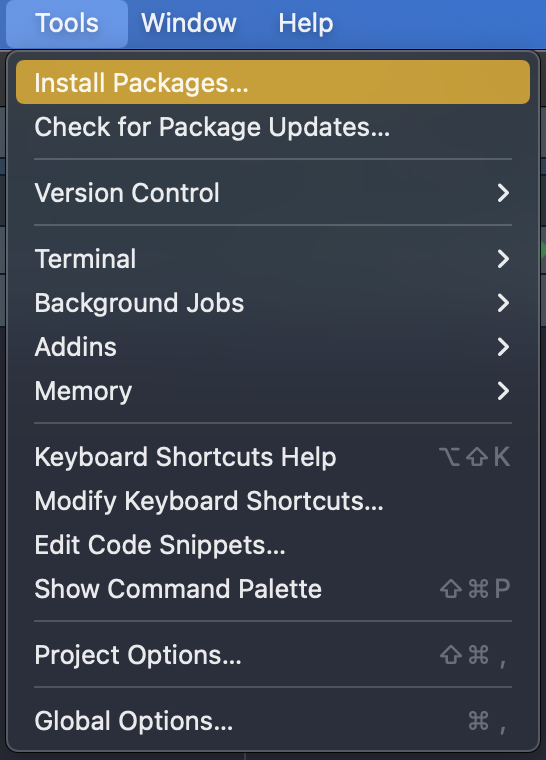
\includegraphics[width=2.84375in,height=\textheight,keepaspectratio]{figures/rlibrerias.png}
\end{center}

La tercera opción es usar el botón ``\textbf{Install}'' dentro de la
pestaña de Packages.

\pandocbounded{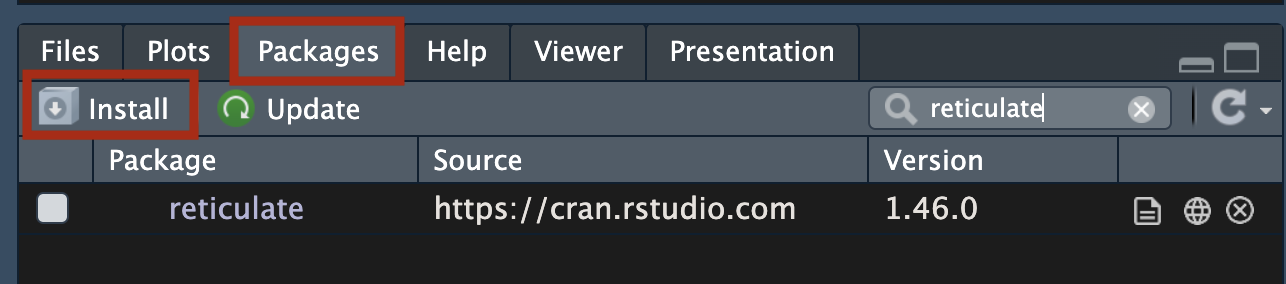
\includegraphics[keepaspectratio]{figures/rlibrerias_paso3.png}}

\subsection{¿Cómo podemos verificar que paquetes
tenemos?}\label{cuxf3mo-podemos-verificar-que-paquetes-tenemos}

En la ventana inferior derecha, existe una pestaña que se llama
``\textbf{Packages}'' que contendra la lista de paquetes instalados en
tu computadora, su descripción corta y su versión.

Tambien en esta pestaña podemos instalar paquetes dandado click en
\textbf{INSTALL}.

\begin{center}
\pandocbounded{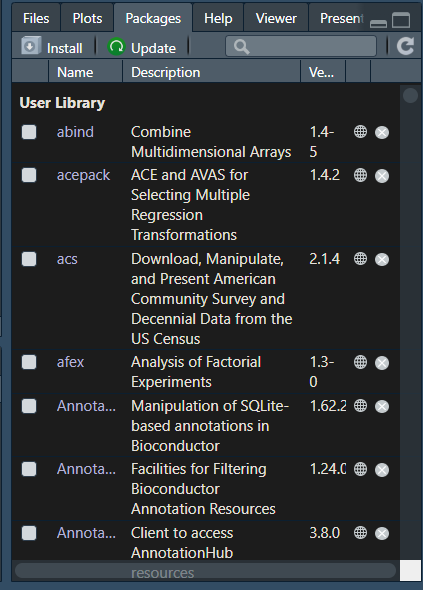
\includegraphics[keepaspectratio]{figures/rlibrerias_paso4.png}}
\end{center}

\subsection{Eliminación de paquetes}\label{eliminaciuxf3n-de-paquetes}

En algunas ocasiones vamos a tener que actualizar las versiones de los
paquetes, pero primero dedes eliminar la versión anterior. Dando click
en el botón que contiene una \texttt{X} que esta al final de la fila en
cada programa.

\begin{center}
\pandocbounded{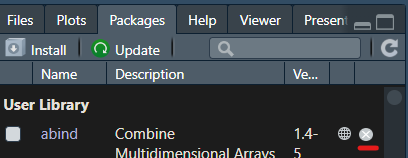
\includegraphics[keepaspectratio]{figures/paquetes_eliminar.png}}
\end{center}

También puedes usar codigo para eliminar el paquete:

\begin{Shaded}
\begin{Highlighting}[]
\FunctionTok{remove.packages}\NormalTok{(}\StringTok{"package{-}to{-}remove"}\NormalTok{)}
\end{Highlighting}
\end{Shaded}

\subsection{Cargar paquetes en el ambiente de
R}\label{cargar-paquetes-en-el-ambiente-de-r}

\begin{itemize}
\tightlist
\item
  \textbf{Opción A:} Emplear la función \texttt{library} para cargar en
  el ambiente el paquete.
\end{itemize}

\begin{Shaded}
\begin{Highlighting}[]
\FunctionTok{library}\NormalTok{(reticulate)}
\end{Highlighting}
\end{Shaded}

\begin{itemize}
\tightlist
\item
  \textbf{Opción B:} Dando click a la \emph{casilla que indica el
  paquete}. Para dejar de usarlo da de nuevo click en esa casilla para
  que deje de estar marcada.
\end{itemize}

\begin{center}
\pandocbounded{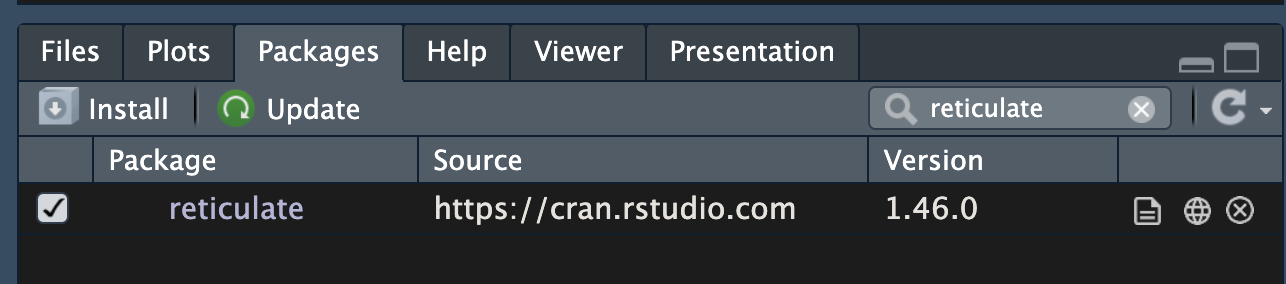
\includegraphics[keepaspectratio]{figures/paquete_cargado.png}}
\end{center}

\chapter{Introducción a Git /
GitHub}\label{introducciuxf3n-a-git-github}

\begin{quote}
\textbf{Fecha:} 06 de octubre, 2026
\end{quote}

\section{¿Por qué hacer control de versiones de nuestros
proyectos?}\label{por-quuxe9-hacer-control-de-versiones-de-nuestros-proyectos}

\begin{enumerate}
\def\labelenumi{\arabic{enumi}.}
\tightlist
\item
  ✅ Los proyectos suelen cambiar y crecer.
\item
  💾 Es díficil saber cuáles fueron todos los cambios a lo largo del
  tiempo (en especial tiempos largos, hazlo por tu yo del
  \textbf{futuro!}).
\item
  🤔 Las colaboraciones se pueden complicar sin un buen control de
  versiones.
\item
  🔐 Seguridad.
\end{enumerate}

\begin{figure}[H]

{\centering \includegraphics[width=3.125in,height=\textheight,keepaspectratio]{index_files/mediabag/phd101212s.png}

}

\caption{``notFinal.doc'' by Jorge Cham, https://www.phdcomics.com}

\end{figure}%

\section{Git}\label{git}

Git es un sistema de \textbf{control de versiones distribuido, gratuito
y de código abierto}, diseñado para manejar todo tipo de proyectos,
desde los más pequeños hasta los más grandes, con rapidez y eficiencia.

Git es fácil de aprender y ocupa poco espacio con un \textbf{rendimiento
rapidísimo}. Supera a las herramientas SCM como Subversion, CVS,
Perforce y ClearCase con características como la ramificación local
barata, las cómodas áreas de preparación y los múltiples flujos de
trabajo.

En resumen:

\begin{itemize}
\item
  Git es un sistema de control de versiones
\item
  Git funciona con GitHub, Bitbucket o GitLab
\end{itemize}

\section{\texorpdfstring{\textbf{Git vs controles de versión a
mano}}{Git vs controles de versión a mano}}\label{git-vs-controles-de-versiuxf3n-a-mano}

\href{https://comunidadbioinfo.github.io/cdsb2023/control-de-versiones-con-github-y-rstudio.html}{\includegraphics[width=6.25in,height=\textheight,keepaspectratio]{index_files/mediabag/git_vers.png}}

Con Git cada contribuidor tiene una copia del repositorio central, con
todos los archivos y la historia de los cambios por los que han pasado.

\section{Recomendaciones para sus
proyectos}\label{recomendaciones-para-sus-proyectos}

\begin{itemize}
\item
  Dedicar un directorio exclusivo por proyecto.
\item
  Es mejor organizarlo en un RStudio Project.
\item
  Hacer un repositorio de Git.
\item
  Trabajen como siempre, solo además de guardar, recuerden hacer
  \texttt{commit}
\item
  De vez en vez hagan \texttt{push} de sus cambios cuando los hayan
  \textbf{verificado}.
\end{itemize}

\section{10.5 Proyectos colaborativos}\label{proyectos-colaborativos}

\begin{itemize}
\item
  GitHub se parece más a un GoogleDoc que a un Word Document.
\item
  Es fácil que los colaboradores hagan cambios y también es fácil saber
  quién hizo que.
\item
  El owner del proyecto puede dar permisos a los diferentes
  colaboradores.
\item
  También existen organizaciones, esto puede ser útil para manejar los
  permisos de grupos grandes de colaboración.
\end{itemize}

\section{GitHub}\label{github}

\href{https://github.com/about}{GitHub} es una plataforma para guardar
proyectos, hace uso de Git. Su principal utilidad es para generar código
fuente de programas.

También existen otras plataformas como
\href{https://bitbucket.org/product/}{Bitbucked} y
\href{https://about.gitlab.com/}{GitLab}, las cuales funcionan de manera
similar a GitHub.

\section{Manual de sobreviviencia con Git Y GitHub en RStudio (en caso
de ser
necesario)}\label{manual-de-sobreviviencia-con-git-y-github-en-rstudio-en-caso-de-ser-necesario}

\begin{itemize}
\item
  Por cualquier problema con la conexión entre RStudio y Git, siempre
  ten en cuenta la ubicación de dónde se instaló Git.

  \begin{itemize}
  \item
    Puedes usar en la terminal \texttt{which\ git} (Mac y Linux)
  \item
    O bien usar en la terminal \texttt{where\ git} (Windows)
  \end{itemize}
\item
  Recuerda que la terminal (línea de comandos, consola, shell o bash) es
  un programa en tu computadora que funciona para correr otros
  programas. Desde RStudio puedes abrir la \textbf{terminal}, lo cual es
  muy conveniente si estás trabajando en un proyecto. Puedes abrir una
  terminal con:

  \begin{itemize}
  \item
    \emph{Tools \textgreater{} Terminal} (abre la terminal dentro del
    IDE de RStudio)
  \item
    \emph{Tools \textgreater{} Shell} (abre una terminal externa a
    RStudio) \textgreater{} Apply \textgreater{} OK
  \end{itemize}
\end{itemize}

\section{Clonar un repositorio y tener conexión/permisos para
modificarlo}\label{clonar-un-repositorio-y-tener-conexiuxf3npermisos-para-modificarlo}

\begin{itemize}
\item
  Git puede comunicarse con un servidor remoto usando uno de dos
  protocolos, HTTPS o SSH, y cada protocolo usa credenciales diferentes.
\item
  La recomendación actual de \textbf{GitHub} es usar HTTPS porque es la
  manera más fácil de configurar y tiene operatividad en múltiples redes
  y plataformas.

  \begin{itemize}
  \item
    Es menos probable que HTTPS sea bloqueado por un firewall.
  \item
    Una conexión HTTPS permite que credential.helper almacene en caché
    su contraseña. (por tanto puedes configurar tu usuario y contraseña
    en tu equipo de uso).
  \item
    Es más sencillo acceder a un repositorio desde cualquier lugar, ya
    que solo necesitas los detalles de tu cuenta (no se requieren claves
    \textbf{SSH}) para escribir en el repositorio.
  \end{itemize}
\item
  Usualmente cuando inicies un proyecto colaborativo con GitHub
  inicializa el repositorio con un README. Copia el HTTPS URL para
  clonar el repositorio en la terminal \texttt{git\ clone}
  \texttt{https://github.com/TU-USUARIO/TU-REPOSITORIO.git}.
\end{itemize}

\section{Referencias}\label{referencias-11}

\begin{itemize}
\tightlist
\item
  Evelia
  tutorial:\href{https://eveliacoss.github.io/Workshop_GitGithub2025/}{Workshop
  sobre Git / Github 2025}
\item
  Haydee tutorial:
  \href{https://haydeeperuyero.github.io/Computo_Cientifico/}{Temas
  Selectos de Análisis Numérico y Computación Científica: Computo
  científico para el análisis de datos}
\item
  Github tutorial:
  \href{https://docs.github.com/es/authentication/connecting-to-github-with-ssh/working-with-ssh-key-passphrases}{Trabajar
  con contraseñas de clave SSH}
\item
  Alejandra Medina tutorial:
  \href{https://comunidadbioinfo.github.io/cdsb2023/control-de-versiones-con-github-y-rstudio.html}{Control
  de versiones con GitHub y RStudio}
\item
  \href{https://ellipse.prbb.org/es/hacia-una-biologia-computacional-mas-reproducible-transparente-y-colaborativa/}{Hacia
  una biología computacional más reproducible, transparente y
  colaborativa}
\end{itemize}

\chapter{Github}\label{github-1}

\begin{quote}
\textbf{Fecha:} 06 de octubre, 2026
\end{quote}

El valor del control de versiones se hace evidente al comenzar a
colaborar con otros. Contamos con la mayor parte de las herramientas
necesarias para ello; lo único que resta es transferir cambios de un
repositorio a otro.

Sistemas como Git posibilitan el traslado de trabajo entre cualquier par
de repositorios. No obstante, en la práctica, resulta más conveniente
utilizar una copia como punto central y mantenerla en la web en lugar de
en la computadora portátil de alguien.

Vamos a comenzar por crear un repositorio remoto, pero para eso
necesitamos configurar nuestra cuenta de Github también.

\section{Paso 1: Crear un repositorio
remoto}\label{paso-1-crear-un-repositorio-remoto}

Lo primero que vamos a hacer es crear un repositorio remoto. Entra a tu
cuenta de Github y dale click en Nuevo.

\begin{figure}[H]

{\centering \includegraphics[width=1.2\linewidth,height=\textheight,keepaspectratio]{index_files/mediabag/github_1.png}

}

\caption{Crear repositorio nuevo}

\end{figure}%

Ponle de nombre \texttt{Mi\_primer\_repo} (o el nombre que hayas usado
en las secciones anteriores). Deja marcada la opción de público y no
añadas un README ni una licencia.

\begin{figure}[H]

{\centering \includegraphics[width=1.2\linewidth,height=\textheight,keepaspectratio]{index_files/mediabag/github_2.png}

}

\caption{Crear repositorio vacío}

\end{figure}%

Al darle click en crear repositorio, la página nos mostrará la siguiente
información que es la que usaremos para configurar nuestro local con el
remoto.

\begin{figure}[H]

{\centering \includegraphics[width=1.2\linewidth,height=\textheight,keepaspectratio]{index_files/mediabag/github_3.png}

}

\caption{Información del repositorio remoto para configurar con nuestro
local}

\end{figure}%

Lo que acabamos de hacer es como si en nuestra terminal hubiéramos
realizado lo siguiente:

\begin{Shaded}
\begin{Highlighting}[]
\FunctionTok{mkdir}\NormalTok{ Mi\_primer\_repo}
\BuiltInTok{cd}\NormalTok{ Mi\_primer\_repo}
\FunctionTok{git}\NormalTok{ init}
\end{Highlighting}
\end{Shaded}

\section{Paso 2: Conectar local a
remoto}\label{paso-2-conectar-local-a-remoto}

La página principal del repositorio remoto muestra una serie de
información que necesitamos usar para conectar el repositorio remoto en
Github con el repositorio local de nuestra computadora. Vamos a usar el
protocolo de conexión SSH, da click en donde dice SSH y a continuación
en el icono de copiar.

\begin{figure}[H]

{\centering \includegraphics[width=1.2\linewidth,height=\textheight,keepaspectratio]{index_files/mediabag/github_4.png}

}

\caption{SSH link para clonar el repositorio}

\end{figure}%

Ahora, dentro de nuestra carpeta del repositorio local, abrir una
terminal y correr lo siguiente:

\begin{Shaded}
\begin{Highlighting}[]
\FunctionTok{git}\NormalTok{ remote add origin git@github.com:User/Mi\_primer\_repo.git}
\end{Highlighting}
\end{Shaded}

Para revisar que si se haya realizado correctamente procedemos a usar lo
siguiente:

\begin{Shaded}
\begin{Highlighting}[]
\FunctionTok{git}\NormalTok{ remote }\AttributeTok{{-}v}
\end{Highlighting}
\end{Shaded}

\section{Paso 3: Conexión mediante
SSH}\label{paso-3-conexiuxf3n-mediante-ssh}

Primero verificamos si ya tenemos algún par de llaves:

\begin{Shaded}
\begin{Highlighting}[]
\FunctionTok{ls} \AttributeTok{{-}al}\NormalTok{ \textasciitilde{}/.ssh}
\end{Highlighting}
\end{Shaded}

Si ya tienen algún par de llaves configuradas las van a ver listadas, si
no tiene ninguna les saldrá una leyenda como la siguiente:

\begin{Shaded}
\begin{Highlighting}[]
\NormalTok{ls: cannot access \textquotesingle{}/c/Users/User/.ssh\textquotesingle{}: No such file or directory}
\end{Highlighting}
\end{Shaded}

\subsection{Paso 3.1: Crear un par de llaves
SSH}\label{paso-3.1-crear-un-par-de-llaves-ssh}

Para crear el par de llaves usamos el siguiente comando, la opción
\texttt{-t} se refiere al tipo de algoritmo usado y la opción
\texttt{-C} indica un comentario para la llave, en este caso el
comentario es nuestro correo.

\begin{Shaded}
\begin{Highlighting}[]
\FunctionTok{ssh{-}keygen} \AttributeTok{{-}t}\NormalTok{ ed25519 }\AttributeTok{{-}C} \StringTok{"email@dominio.com"}
\end{Highlighting}
\end{Shaded}

Si tu sistema operativo no lo permite, usa
\texttt{ssh-keygen\ -t\ rsa\ -b\ 4096\ -C\ "your\_email@example.com"}.

\textbf{Nota:} Si no cuentas con \texttt{ssh-keygen} instalado, primero
corre el código:

\begin{Shaded}
\begin{Highlighting}[]
\FunctionTok{sudo}\NormalTok{ apt{-}get install ssh{-}keygen}
\end{Highlighting}
\end{Shaded}

Como queremos usar el archivo default, solo damos Enter. Ahora nos
pedirá una contraseña, tecleala, no vas a ver nada en la pantalla. Una
vez creada verás en pantalla algo como lo siguiente:

\begin{Shaded}
\begin{Highlighting}[]
\ExtensionTok{Your}\NormalTok{ identification has been saved in /c/Users/user/.ssh/id\_ed25519}
\ExtensionTok{Your}\NormalTok{ public key has been saved in /c/Users/user/.ssh/id\_ed25519.pub}
\ExtensionTok{The}\NormalTok{ key fingerprint is:}
\ExtensionTok{SHA256:SMSPIStNyA10KPxuYu94KpZg9AYjgt9g46A4kFy3g1o}\NormalTok{ user@domain}
\ExtensionTok{The}\NormalTok{ keys randomart image is:}
\ExtensionTok{+{-}{-}[ED25519}\NormalTok{ 256]{-}{-}+}
\KeywordTok{|}\ExtensionTok{\^{}B==}\NormalTok{ o.          }\KeywordTok{|}
\KeywordTok{|}\ExtensionTok{\%*=} \PreprocessorTok{*}\NormalTok{.+          }\KeywordTok{|}
\KeywordTok{|}\ExtensionTok{+=.E}\NormalTok{ =.+         }\KeywordTok{|}
\KeywordTok{|} \BuiltInTok{.}\NormalTok{=.+.o..        }\KeywordTok{|}
\KeywordTok{|}\ExtensionTok{...}\NormalTok{   . S        }\KeywordTok{|}
\KeywordTok{|}\BuiltInTok{.}\NormalTok{+ o             }\KeywordTok{|}
\KeywordTok{|}\ExtensionTok{+}\NormalTok{ =              }\KeywordTok{|}
\KeywordTok{|}\ExtensionTok{.o.o}             \KeywordTok{|}
\KeywordTok{|}\ExtensionTok{oo+.}             \KeywordTok{|}
\ExtensionTok{+{-}{-}{-}{-}[SHA256]{-}{-}{-}{-}{-}+}
\end{Highlighting}
\end{Shaded}

Lo que dice \texttt{identification} ser refiere a la llave privada la
cual no debes compartir nunca y la cadena de caracteres que dice
\texttt{fingerprint} se refiere a parte de tu llave pública.

Si repetimos el comando siguiente, verán ahora ya sus dos claves pública
y privada.

\begin{Shaded}
\begin{Highlighting}[]
\FunctionTok{ls} \AttributeTok{{-}al}\NormalTok{ \textasciitilde{}/.ssh}
\end{Highlighting}
\end{Shaded}

\subsection{Paso 3.2 Generar una llave pública exclusiva para Github
(opcional)}\label{paso-3.2-generar-una-llave-puxfablica-exclusiva-para-github-opcional}

En caso de que ya cuentes con una llave con ese nombre, puedes crear una
nueva llave con otro nombre especifico para Github:

\begin{Shaded}
\begin{Highlighting}[]
\FunctionTok{ssh{-}keygen} \AttributeTok{{-}t}\NormalTok{ ed25519 }\AttributeTok{{-}C} \StringTok{"your\_email@example.com"} \AttributeTok{{-}f}\NormalTok{ \textasciitilde{}/.ssh/id\_ed25519\_github}
\end{Highlighting}
\end{Shaded}

\begin{figure}[H]

{\centering \includegraphics[width=3.125in,height=\textheight,keepaspectratio]{index_files/mediabag/Clave_github.jpg}

}

\caption{Clave exclusiva de github}

\end{figure}%

Ahora que ya tenemos las claves, debemos decirle a GitHub cuales son.

\begin{Shaded}
\begin{Highlighting}[]
\FunctionTok{cat}\NormalTok{ \textasciitilde{}/.ssh/id\_ed25519.pub}
\end{Highlighting}
\end{Shaded}

Copia la cadena de caracteres, ve a la configuración de tu perfil de
GitHub y da clic en ``SSH and GPG Keys''.

\begin{figure}[H]

{\centering \includegraphics[width=1.2\linewidth,height=\textheight,keepaspectratio]{index_files/mediabag/github_5.png}

}

\caption{SSH and GPG Keys}

\end{figure}%

Una vez ahí da clic en ``Nueva llave SSH''.

\begin{figure}[H]

{\centering \includegraphics[width=1.2\linewidth,height=\textheight,keepaspectratio]{index_files/mediabag/github_6.png}

}

\caption{Nueva llave SSH}

\end{figure}%

Después coloca un título que te permita identificar que será la clave
con la que usarás la computadora y pega tu llave pública.

\begin{figure}[H]

{\centering \includegraphics[width=1.2\linewidth,height=\textheight,keepaspectratio]{index_files/mediabag/github_7.png}

}

\caption{Llave pública}

\end{figure}%

Ahora solo falta revisar la conexión desde la terminal.

\begin{Shaded}
\begin{Highlighting}[]
\FunctionTok{ssh} \AttributeTok{{-}T}\NormalTok{ git@github.com}
\end{Highlighting}
\end{Shaded}

Si vez un mensaje similar al siguiente, significa que quedo completa la
autenticación.

\begin{Shaded}
\begin{Highlighting}[]
\ExtensionTok{Hi}\NormalTok{ Name! Youve successfully authenticated, but GitHub does not provide shell access.}
\end{Highlighting}
\end{Shaded}

\subsection{Paso 3.3 Solución a Error con la
llave}\label{paso-3.3-soluciuxf3n-a-error-con-la-llave}

A mi paso que la llave esta bien pero no tenia acceso a usar github,
mostrando este mensaje:

\begin{verbatim}
ssh -i .ssh/id_ed25519 -T git@github.com
Hi HaydeePeruyero! You've successfully authenticated, but GitHub does not provide shell access.
\end{verbatim}

\subsubsection{Agregar configuración}\label{agregar-configuraciuxf3n}

Por lo que decidí configurar el archivo
\texttt{\textasciitilde{}/.ssh/config}.

\begin{Shaded}
\begin{Highlighting}[]
\FunctionTok{nano}\NormalTok{ \textasciitilde{}/.ssh/config}
\end{Highlighting}
\end{Shaded}

agrega esto:

\begin{Shaded}
\begin{Highlighting}[]
\ExtensionTok{Host}\NormalTok{ github.com}
  \ExtensionTok{HostName}\NormalTok{ github.com}
  \ExtensionTok{User}\NormalTok{ git}
  \ExtensionTok{IdentityFile}\NormalTok{ \textasciitilde{}/.ssh/id\_ed25519}
  \ExtensionTok{IdentitiesOnly}\NormalTok{ yes}
\end{Highlighting}
\end{Shaded}

Guarda y cierra las modificaciones del archivo.

\subsubsection{Verifica que los permisos estén
correctos}\label{verifica-que-los-permisos-estuxe9n-correctos}

\begin{Shaded}
\begin{Highlighting}[]
\FunctionTok{chmod}\NormalTok{ 600 \textasciitilde{}/.ssh/id\_ed25519}
\FunctionTok{chmod}\NormalTok{ 644 \textasciitilde{}/.ssh/id\_ed25519.pub}
\FunctionTok{chmod}\NormalTok{ 600 \textasciitilde{}/.ssh/config}
\end{Highlighting}
\end{Shaded}

\subsubsection{\texorpdfstring{\textbf{Agrega tu clave al
\texttt{ssh-agent}}}{Agrega tu clave al ssh-agent}}\label{agrega-tu-clave-al-ssh-agent}

Esto asegura que la clave esté disponible durante tus sesiones:

\begin{Shaded}
\begin{Highlighting}[]
\FunctionTok{ssh{-}add}\NormalTok{ \textasciitilde{}/.ssh/id\_ed25519}
\end{Highlighting}
\end{Shaded}

\subsubsection{Prueba conexión otra
vez}\label{prueba-conexiuxf3n-otra-vez}

\begin{Shaded}
\begin{Highlighting}[]
\FunctionTok{ssh} \AttributeTok{{-}T}\NormalTok{ git@github.com}
\end{Highlighting}
\end{Shaded}

Debe decir:

\begin{Shaded}
\begin{Highlighting}[]
\ExtensionTok{Hi}\NormalTok{ HaydeePeruyero! You}\StringTok{\textquotesingle{}ve successfully authenticated, but GitHub does not provide shell access.}
\end{Highlighting}
\end{Shaded}

\section{Paso 4: Push and pull}\label{paso-4-push-and-pull}

Una vez que ya tenemos configurado todo, solo falta enviar todo lo que
tenemos en el repo local al remoto. Si se establecio la contraseña nos
la va a pedir en la terminal o una ventana aparte.

\begin{Shaded}
\begin{Highlighting}[]
\FunctionTok{git}\NormalTok{ push origin main}
\end{Highlighting}
\end{Shaded}

En esa instrucción, \texttt{origin} se refiere al repositorio remoto y
\texttt{main} al local (las ramas que estamos intentando poner en el
mismo contenido).

La situación en la que estamos es la siguiente:

\begin{figure}[H]

{\centering \includesvg[width=1.2\linewidth,height=\textheight,keepaspectratio]{index_files/mediabag/github-repo-after-fi.svg}

}

\caption{git push origin main}

\end{figure}%

Para actualizar nuestro repositorio local, lo que debemos hacer es lo
siguiente:

\begin{Shaded}
\begin{Highlighting}[]
\FunctionTok{git}\NormalTok{ pull origin main}
\end{Highlighting}
\end{Shaded}

Como no hemos realizado ningún cambio en el remoto, no veremos nada
nuevo en el local. En el remoto también podemos añadir archivos
directamente.

\begin{tcolorbox}[enhanced jigsaw, arc=.35mm, bottomrule=.15mm, bottomtitle=1mm, breakable, colback=white, colbacktitle=quarto-callout-note-color!10!white, colframe=quarto-callout-note-color-frame, coltitle=black, left=2mm, leftrule=.75mm, opacityback=0, opacitybacktitle=0.6, rightrule=.15mm, title=\textcolor{quarto-callout-note-color}{\faInfo}\hspace{0.5em}{Ejercicio}, titlerule=0mm, toprule=.15mm, toptitle=1mm]

Añade un archivo nuevo desde el repositorio remoto y actualiza tus
cambios en el local.

\begin{quote}
\textbf{Solución}

Desde el repositorio remoto, podemos crear un nuevo archivo, por ejemplo
\texttt{nuevo\_archivo.txt}, escribir algo en él y guardar los cambios.
GitHub realizará automáticamente un commit en el repositorio remoto.

Ahora, en nuestra copia local, verificamos el estado del repositorio:

\begin{Shaded}
\begin{Highlighting}[]
\FunctionTok{git}\NormalTok{ status}
\end{Highlighting}
\end{Shaded}

y descargamos los cambios del repositorio remoto con:

\begin{Shaded}
\begin{Highlighting}[]
\FunctionTok{git}\NormalTok{ pull origin main}
\end{Highlighting}
\end{Shaded}

(En caso de que la rama principal tenga otro nombre, reemplazar
\texttt{main} por el nombre correspondiente.)

Git descargará e integrará automáticamente el nuevo commit en nuestro
repositorio local.

Podemos comprobar que el archivo se ha añadido con:

\begin{Shaded}
\begin{Highlighting}[]
\FunctionTok{ls}
\end{Highlighting}
\end{Shaded}

o revisar el historial con:

\begin{Shaded}
\begin{Highlighting}[]
\FunctionTok{git}\NormalTok{ log }\AttributeTok{{-}{-}oneline}
\end{Highlighting}
\end{Shaded}

Observaremos que ahora el commit realizado desde GitHub también aparece
en el historial local.
\end{quote}

\end{tcolorbox}

\chapter{Conectar a GitHub con SSH}\label{conectar-a-github-con-ssh}

\begin{quote}
\textbf{Fecha:} 06 de octubre, 2026
\end{quote}

Puedes conectarte a GitHub utilizando el \textbf{protocolo Secure Shell
(SSH)}, lo cual proporciona un canal seguro sobre una red insegura.

También puedes asegurar tus claves SSH y configurar un agente de
autenticación para no tener que ingresar tu contraseña cada vez que
utilices tus claves SSH.

\section{Paso 1. Generar una llave
pública}\label{paso-1.-generar-una-llave-puxfablica}

\begin{tcolorbox}[enhanced jigsaw, arc=.35mm, bottomrule=.15mm, bottomtitle=1mm, breakable, colback=white, colbacktitle=quarto-callout-note-color!10!white, colframe=quarto-callout-note-color-frame, coltitle=black, left=2mm, leftrule=.75mm, opacityback=0, opacitybacktitle=0.6, rightrule=.15mm, title=\textcolor{quarto-callout-note-color}{\faInfo}\hspace{0.5em}{Actividad (15 min)}, titlerule=0mm, toprule=.15mm, toptitle=1mm]

Deberan contar con:

\begin{enumerate}
\def\labelenumi{\arabic{enumi}.}
\item
  Una cuenta en GitHub
\item
  \textbf{R} y \textbf{RStudio} actualizados
\item
  \href{https://miguel-mx.github.io/2024-01-24-ccm-unam-swc/\#the-bash-shell}{Git
  instalado}
\item
  Coloca en la terminal la siguiente información para generar una clave
  con el mismo correo que usaste para registrar tu cuenta en GitHub.

\begin{Shaded}
\begin{Highlighting}[]
\FunctionTok{ssh{-}keygen} \AttributeTok{{-}t}\NormalTok{ ed25519 }\AttributeTok{{-}C} \StringTok{"your\_email@example.com"}
\end{Highlighting}
\end{Shaded}

  NOTA: Si no cuentas con \texttt{ssh-keygen} instalado, primero corre
  este código.

\begin{verbatim}
sudo apt-get install ssh-keygen
\end{verbatim}
\end{enumerate}

\end{tcolorbox}

Cuando ejecutes el programa, te va a preguntar si quieres generar una
frase, identificar y como quieres nombrar la llave. Si no quieres
complicarte presiona \textbf{3 veces ENTER}, hasta que te parezca una
pantalla como al siguiente:

\pandocbounded{\includegraphics[keepaspectratio]{figures/Clave_ed25519.jpg}}

Posteriormente, tendras una carpeta llamada \texttt{.ssh/}, entra en esa
carpeta y tendras dos archivos, si no los renombraste tendran el nombre
de \texttt{id\_ed25519}.

\begin{itemize}
\item
  \texttt{id\_ed25519}: llave local, no la vamos a usar. Tampoco la
  compartas.
\item
  \texttt{id\_ed25519.pub} : llave publica. La usaremos para copiarla en
  los servidores que usaremos.
\end{itemize}

Vamos a abrir la terminal y vamos a ver el contenido de la carpeta
\texttt{.ssh/}:

\begin{Shaded}
\begin{Highlighting}[]
\FunctionTok{ls}\NormalTok{ .ssh/}
\end{Highlighting}
\end{Shaded}

\section{Paso 1. Generar una llave pública exclusiva para Github
(opcional)}\label{paso-1.-generar-una-llave-puxfablica-exclusiva-para-github-opcional}

En caso de que ya cuentes con una clase con ese nombre, puedes crear una
nueva llave con otro nombre especifico para Github:

\begin{Shaded}
\begin{Highlighting}[]
\FunctionTok{ssh{-}keygen} \AttributeTok{{-}t}\NormalTok{ ed25519 }\AttributeTok{{-}C} \StringTok{"your\_email@example.com"} \AttributeTok{{-}f}\NormalTok{ \textasciitilde{}/.ssh/id\_ed25519\_github}
\end{Highlighting}
\end{Shaded}

\pandocbounded{\includegraphics[keepaspectratio]{figures/Clave_github.jpg}}

\section{Paso 2. Copiar la clave SSH
pública}\label{paso-2.-copiar-la-clave-ssh-puxfablica}

\begin{enumerate}
\def\labelenumi{\arabic{enumi}.}
\tightlist
\item
  Accede a la terminal en tu computadora.
\item
  Copia la clave SSH generada anteriormente usando el siguiente comando:
\end{enumerate}

\begin{Shaded}
\begin{Highlighting}[]
\FunctionTok{cat}\NormalTok{ \textasciitilde{}/.ssh/id\_ed25519.pub}
\end{Highlighting}
\end{Shaded}

Este comando mostrará tu clave pública en la terminal.

\begin{enumerate}
\def\labelenumi{\arabic{enumi}.}
\setcounter{enumi}{2}
\tightlist
\item
  Selecciona y copia toda la clave que aparece en la terminal. Asegúrate
  de copiar desde ssh-rsa hasta el final de tu correo electrónico.
\end{enumerate}

\section{Paso 3. Agregar la clave SSH a tu cuenta de
GitHub}\label{paso-3.-agregar-la-clave-ssh-a-tu-cuenta-de-github}

\begin{enumerate}
\def\labelenumi{\arabic{enumi}.}
\tightlist
\item
  Inicia sesión en GitHub en tu navegador.
\item
  Haz clic en tu foto de perfil en la esquina superior derecha y
  selecciona \textbf{``Settings''} (Configuración).
\item
  En el menú lateral izquierdo, selecciona \textbf{``SSH and GPG
  keys''}.
\item
  Haz clic en el botón verde \textbf{``New SSH key''}.
\item
  En el campo \textbf{``Title''}, ingresa un nombre descriptivo para tu
  clave (por ejemplo, ``Mi computadora personal'').
\item
  En el campo \textbf{``Key''}, pega la clave SSH que copiaste
  previamente de la terminal.
\item
  Haz clic en \textbf{``Add SSH key''} para guardar la clave.
\end{enumerate}

\section{Paso 4. Configurar RStudio para usar Git Bash como
terminal}\label{paso-4.-configurar-rstudio-para-usar-git-bash-como-terminal}

\begin{enumerate}
\def\labelenumi{\arabic{enumi}.}
\item
  Abre \textbf{RStudio}.
\item
  Dirígete a \textbf{Tools} (Herramientas) en la barra superior y
  selecciona \textbf{Global Options} (Opciones globales).
\item
  En el menú de opciones globales, selecciona la pestaña
  \textbf{Terminal}.
\item
  En el campo \textbf{New terminal open with}, selecciona \textbf{Git
  Bash}.

  \pandocbounded{
\includegraphics[keepaspectratio]{figures/Rstudio_GitBash.jpg}}
\item
  Haz clic en \textbf{Apply} y luego en \textbf{OK}.
\end{enumerate}

\section{Paso 5. Abrir la terminal de Git Bash en
RStudio}\label{paso-5.-abrir-la-terminal-de-git-bash-en-rstudio}

Ahora, para abrir la terminal de \textbf{Git Bash dentro de RStudio},
solo tienes que:

\begin{itemize}
\item
  Ir al \textbf{Tools} , hacer clic en \textbf{Terminal} y en abrir
  \textbf{New terminal}.
\item
  Deberías ver que se abre una nueva sesión con \textbf{Git Bash} como
  la terminal predeterminada.
\end{itemize}

\section{Paso 6. Verificar la
conexión}\label{paso-6.-verificar-la-conexiuxf3n}

Vuelve a la terminal y ejecuta el siguiente comando para verificar que
tu clave SSH está correctamente configurada con GitHub:

\begin{Shaded}
\begin{Highlighting}[]
\FunctionTok{ssh} \AttributeTok{{-}T}\NormalTok{ git@github.com}
\end{Highlighting}
\end{Shaded}

En caso de que se necesite, puedes especificar la llave que usaste:

\begin{Shaded}
\begin{Highlighting}[]
\FunctionTok{ssh} \AttributeTok{{-}i}\NormalTok{ \textasciitilde{}/.ssh/id\_ed25519 }\AttributeTok{{-}T}\NormalTok{ git@github.com}
\end{Highlighting}
\end{Shaded}

El comando \texttt{ssh\ -T\ git@github.com} simplemente verifica que tu
clave privada se está usando correctamente y que tu clave pública ha
sido registrada en GitHub.

Si es la primera vez que te conectas a GitHub con SSH, puede que veas un
mensaje que te pregunte si deseas continuar conectándote. Escribe
``yes''.

Si todo está bien configurado, deberías ver un mensaje similar a este:

\begin{verbatim}
Hi username! You've successfully authenticated, but GitHub does not provide shell access.
\end{verbatim}

Esto confirmará que tu clave SSH se ha agregado correctamente a tu
cuenta de GitHub y que la conexión es exitosa.

\subsection{Solución a Error con la
llave}\label{soluciuxf3n-a-error-con-la-llave}

A mi paso que la llave esta bien pero no tenia acceso a usar github,
mostrando este mensaje:

\begin{verbatim}
ssh -i .ssh/id_ed25519_github -T git@github.com
Hi EveliaCoss! You've successfully authenticated, but GitHub does not provide shell access.
\end{verbatim}

\subsubsection{Agregar configuración}\label{agregar-configuraciuxf3n-1}

Por lo que decidi configurar el archivo
\texttt{\textasciitilde{}/.ssh/config}.

\begin{Shaded}
\begin{Highlighting}[]
\FunctionTok{nano}\NormalTok{ \textasciitilde{}/.ssh/config}
\end{Highlighting}
\end{Shaded}

agrega esto:

\begin{Shaded}
\begin{Highlighting}[]
\ExtensionTok{Host}\NormalTok{ github.com}
  \ExtensionTok{HostName}\NormalTok{ github.com}
  \ExtensionTok{User}\NormalTok{ git}
  \ExtensionTok{IdentityFile}\NormalTok{ \textasciitilde{}/.ssh/id\_ed25519\_github}
  \ExtensionTok{IdentitiesOnly}\NormalTok{ yes}
\end{Highlighting}
\end{Shaded}

Guarda y cierra las modificaciones del archivo.

\subsubsection{Verifica que los permisos estén
correctos}\label{verifica-que-los-permisos-estuxe9n-correctos-1}

\begin{Shaded}
\begin{Highlighting}[]
\FunctionTok{chmod}\NormalTok{ 600 \textasciitilde{}/.ssh/id\_ed25519\_github}
\FunctionTok{chmod}\NormalTok{ 644 \textasciitilde{}/.ssh/id\_ed25519\_github.pub}
\FunctionTok{chmod}\NormalTok{ 600 \textasciitilde{}/.ssh/config}
\end{Highlighting}
\end{Shaded}

\subsubsection{\texorpdfstring{\textbf{Agrega tu clave al
\texttt{ssh-agent}}}{Agrega tu clave al ssh-agent}}\label{agrega-tu-clave-al-ssh-agent-1}

Esto asegura que la clave esté disponible durante tus sesiones:

\begin{Shaded}
\begin{Highlighting}[]
\FunctionTok{ssh{-}add}\NormalTok{ \textasciitilde{}/.ssh/id\_ed25519\_github}
\end{Highlighting}
\end{Shaded}

\subsubsection{Prueba conexión otra
vez}\label{prueba-conexiuxf3n-otra-vez-1}

\begin{Shaded}
\begin{Highlighting}[]
\FunctionTok{ssh} \AttributeTok{{-}T}\NormalTok{ git@github.com}
\end{Highlighting}
\end{Shaded}

Debe decir:

\begin{Shaded}
\begin{Highlighting}[]
\ExtensionTok{Hi}\NormalTok{ EveliaCoss! You}\StringTok{\textquotesingle{}ve successfully authenticated, but GitHub does not provide shell access.}
\end{Highlighting}
\end{Shaded}

\subsection{Solución a Error con la Configuración del Usuario en
Git}\label{soluciuxf3n-a-error-con-la-configuraciuxf3n-del-usuario-en-git}

El comando \texttt{git\ config} se utiliza para configurar opciones en
Git, y los siguientes comandos en particular se usan para establecer tu
nombre y correo electrónico globalmente en tu configuración de Git:

\begin{verbatim}
git config --global user.email "you@example.com"
git config --global user.name "Your Name"
\end{verbatim}

\begin{enumerate}
\def\labelenumi{\arabic{enumi}.}
\tightlist
\item
  \texttt{git\ config\ -\/-global\ user.email\ "you@example.com"}
\end{enumerate}

Este comando configura tu dirección de correo electrónico, la cual será
utilizada en todos tus commits de Git. El correo electrónico asociado
con los commits es importante porque ayuda a identificar quién realizó
qué cambios en el repositorio. --global significa que esta configuración
se aplicará a todos los repositorios en tu máquina.

\begin{enumerate}
\def\labelenumi{\arabic{enumi}.}
\setcounter{enumi}{1}
\tightlist
\item
  \texttt{git\ config\ -\/-global\ user.name\ "Your\ Name"}
\end{enumerate}

Este comando establece tu nombre de usuario, que también se asociará con
los commits que realices. Al igual que el correo electrónico, se
utilizará en todos tus commits en cualquier repositorio de Git en tu
máquina.

\section{Referencias}\label{referencias-12}

\begin{itemize}
\tightlist
\item
  Haydee tutorial:
  \href{https://haydeeperuyero.github.io/Computo_Cientifico/}{Temas
  Selectos de Análisis Numérico y Computación Científica: Computo
  científico para el análisis de datos}
\item
  Alejandra Medina tutorial:
  \href{https://comunidadbioinfo.github.io/cdsb2023/control-de-versiones-con-github-y-rstudio.html}{Control
  de versiones con GitHub y RStudio}
\end{itemize}

\chapter{Configurar Git}\label{configurar-git}

\begin{quote}
\textbf{Fecha:} 06 de octubre, 2026
\end{quote}

Usar control de versiones es una forma de manejar proyectos, todo a lo
que se hace \texttt{commit} no se pierde, se queda un registro de todos
los cambios y siempre es posible regresar a una versión anterior. Nos
evitamos estar enviando y enviando correos con versiones finales para
después comparar versiones. Se guarda el usuario que hizo el cambio y
automáticamente obtenemos una notificación de si intentamos modificar lo
mismo que un colaborador para revisar cual cambio guardar.

Pueden pensar en versión de control como una forma de \texttt{undo}
ilimitado y de trabajar paralelamente con sus colaboradores.

Lo primero que vamos a hacer es configurar \texttt{Git} en nuestra
computadora.

Vamos a abrir \texttt{Git\ bash} y configurar nuestro usuario y correo
con la que vamos a enlazar más adelante Github.

\begin{Shaded}
\begin{Highlighting}[]
\FunctionTok{git}\NormalTok{ config }\AttributeTok{{-}{-}global}\NormalTok{ user.name }\StringTok{"Usuario"}
\FunctionTok{git}\NormalTok{ config }\AttributeTok{{-}{-}global}\NormalTok{ user.email }\StringTok{"email@domain.com"}
\end{Highlighting}
\end{Shaded}

Ahora, vamos a configurar los saltos de línea para no tener conflicto
según el sistema operativo.

\begin{Shaded}
\begin{Highlighting}[]
\CommentTok{\# Mac o Linux}
\FunctionTok{git}\NormalTok{ config }\AttributeTok{{-}{-}global}\NormalTok{ core.autocrlf input}
\CommentTok{\# Windows}
\FunctionTok{git}\NormalTok{ config }\AttributeTok{{-}{-}global}\NormalTok{ core.autocrlf true}
\end{Highlighting}
\end{Shaded}

Para configurar el editor de texto por default:

\begin{Shaded}
\begin{Highlighting}[]
\FunctionTok{git}\NormalTok{ config }\AttributeTok{{-}{-}global}\NormalTok{ core.editor }\StringTok{"nano {-}w"}
\end{Highlighting}
\end{Shaded}

Por default, Git inicializa un repositorio con una rama llamada
\texttt{master}, a partir del 2020, la mayoría de los servidores de Git
cambiaron esto a que la rama principal fuera \texttt{main}, para
configurar esto usaremos lo siguiente:

\begin{Shaded}
\begin{Highlighting}[]
\FunctionTok{git}\NormalTok{ config }\AttributeTok{{-}{-}global}\NormalTok{ init.defaultBranch main}
\end{Highlighting}
\end{Shaded}

Los comandos anteriores solo se necesitan configurar una sola vez. Para
ver la configuración que acabamos de realizar y probar cual es nuestro
editor de texto usamos lo siguiente:

\begin{Shaded}
\begin{Highlighting}[]
\FunctionTok{git}\NormalTok{ config }\AttributeTok{{-}{-}global} \AttributeTok{{-}{-}edit}
\end{Highlighting}
\end{Shaded}

Y para revisar esta configuración sin entrar al editor:

\begin{Shaded}
\begin{Highlighting}[]
\FunctionTok{git}\NormalTok{ config }\AttributeTok{{-}{-}list}
\end{Highlighting}
\end{Shaded}

Si debieran hacer cambios en su usuario o correo o cualquier otra
configuración lo pueden hacer ilimitadas veces con los comandos
anteriores.

Para pedir ayuda nos sirve aún \texttt{git\ comando\ -h} o
\texttt{git\ comando\ -\/-help}, por ejemplo:

\begin{Shaded}
\begin{Highlighting}[]
\FunctionTok{git}\NormalTok{ config }\AttributeTok{{-}h}
\end{Highlighting}
\end{Shaded}

La siguiente nos abre en un navegador el manual completo:

\begin{Shaded}
\begin{Highlighting}[]
\FunctionTok{git}\NormalTok{ config }\AttributeTok{{-}{-}help}
\end{Highlighting}
\end{Shaded}

O para ayuda general de Git: \texttt{git\ help}.

\chapter{Introducción a Quarto}\label{introducciuxf3n-a-quarto}

\begin{quote}
\textbf{Fecha:} 13 de octubre, 2026
\end{quote}

\textbf{Quarto} es una versión multilingüe y
\href{https://quarto.org/docs/faq/rmarkdown.html}{de última generación}
de R Markdown de Posit que incluye docenas de nuevas características y
capacidades y al mismo tiempo puede renderizar la mayoría de los
archivos Rmd existentes sin modificaciones.

\begin{itemize}
\tightlist
\item
  Extensión \texttt{.qmd}
\item
  Sintaxis de Markdown para el texto
\item
  Tipos de archivos puede ser \hyperref[0]{HTML} , \hyperref[0]{PDF} ,
  documento \hyperref[0]{de MS Word , presentación} , \hyperref[0]{sitio
  web} , \hyperref[0]{libro} , \hyperref[0]{documento interactivo} u
  \hyperref[0]{otro formato} .
\end{itemize}

\begin{center}
\pandocbounded{\includegraphics[keepaspectratio]{images/clipboard-2661750054.png}}
\end{center}

\section{¿Cómo funciona?}\label{cuxf3mo-funciona}

Utiliza el botón
\includegraphics[width=0.20833in,height=0.17708in]{index_files/mediabag/rstudio-render-butto.png}
\textbf{Render} en el IDE de RStudio para renderizar el archivo y
obtener una vista previa de la salida con un solo clic o un atajo de
teclado (⇧⌘K).

\pandocbounded{\includegraphics[keepaspectratio]{images/clipboard-3479006155.png}}

Si prefiere renderizar automáticamente al guardar, puede activar la
opción ``Renderizar al guardar'' en la barra de herramientas del editor.
La vista previa se actualizará al volver a renderizar el documento. La
vista previa en paralelo funciona tanto con HTML como con PDF.

\pandocbounded{\includegraphics[keepaspectratio]{images/clipboard-2728400971.png}}

Al renderizar un documento de Quarto,
\href{http://yihui.name/knitr/}{knitr} ejecuta primero todos los
fragmentos de código y crea un nuevo documento Markdown (.md), que
incluye el código y su salida. El archivo Markdown generado es procesado
por \href{http://pandoc.org/}{pandoc} , que crea el formato final. El
botón Renderizar encapsula estas acciones y las ejecuta en el orden
correcto.

\pandocbounded{\includegraphics[keepaspectratio]{images/clipboard-318997387.png}}

\section{¿Cómo se compone?}\label{cuxf3mo-se-compone}

El archivo contiene tres tipos de contenido: \textbf{un encabezado YAML,
fragmentos de código} y \textbf{texto Markdown}.

\subsection{\texorpdfstring{\textbf{encabezado
YAML}}{encabezado YAML}}\label{encabezado-yaml}

Un encabezado YAML (opcional) delimitado por tres guiones (
\texttt{-\/-\/-}) en cada extremo.

\begin{verbatim}
---
title: "Hello, Quarto"
format: html
editor: visual
---
\end{verbatim}

Al renderizar, el símbolo \texttt{title}, \texttt{"Hello,\ Quarto"},
aparecerá en la parte superior del documento renderizado con un tamaño
de fuente mayor que el resto del documento. Los otros dos campos YAML
indican que la salida debe estar en formato \texttt{html}
\texttt{format}y que el documento debe abrirse en formato
\texttt{visual} \texttt{editor}predeterminado.

Puedes consultar todos los campos YAML disponibles para documentos: HTML
\href{https://quarto.org/docs/reference/formats/html.html}{aquí} . Los
campos YAML disponibles varían según el formato del documento; por
ejemplo, consulte
\href{https://quarto.org/docs/reference/formats/pdf.html}{aquí} los
campos YAML para documentos PDF y
\href{https://quarto.org/docs/reference/formats/docx.html}{aquí} para MS
Word.

\begin{tcolorbox}[enhanced jigsaw, arc=.35mm, bottomrule=.15mm, bottomtitle=1mm, breakable, colback=white, colbacktitle=quarto-callout-important-color!10!white, colframe=quarto-callout-important-color-frame, coltitle=black, left=2mm, leftrule=.75mm, opacityback=0, opacitybacktitle=0.6, rightrule=.15mm, title=\textcolor{quarto-callout-important-color}{\faExclamation}\hspace{0.5em}{Importante}, titlerule=0mm, toprule=.15mm, toptitle=1mm]

Para crear archivos PDF, se necesitará instalar una distribución
reciente de \href{https://www.latex-project.org/}{LaTeX}. Recomendamos
usar TinyTeX (basado en TexLive), que se puede instalar con el siguiente
comando:

\begin{Shaded}
\begin{Highlighting}[]
\ExtensionTok{quarto}\NormalTok{ install tinytex}
\end{Highlighting}
\end{Shaded}

\end{tcolorbox}

\section{Renderizar a varios tipos de
archivos}\label{renderizar-a-varios-tipos-de-archivos}

Si desea renderizar en todos los formatos, puede hacerlo con el paquete
\href{https://github.com/quarto-dev/quarto-r}{\textbf{quarto}} , que
proporciona una interfaz de R para la CLI de Quarto. Por ejemplo, para
renderizar el documento actual, utilice
\texttt{quarto::quarto\_render()}. También puede especificar el nombre
del documento que desea renderizar, así como los formatos de salida.

\begin{Shaded}
\begin{Highlighting}[]
\ExtensionTok{quarto::quarto\_render}\ErrorTok{(}
  \StringTok{"authoring.qmd"}\ExtensionTok{,} 
  \ExtensionTok{output\_format}\NormalTok{ = c}\ErrorTok{(}\StringTok{"pdf"}\ExtensionTok{,} \StringTok{"html"}\NormalTok{, }\StringTok{"docx"}\KeywordTok{)}
\KeywordTok{)}
\end{Highlighting}
\end{Shaded}

Como resultado, verá aparecer tres nuevos archivos en el panel Archivos:

\begin{itemize}
\tightlist
\item
  \texttt{authoring.docx}
\item
  \texttt{authoring.html}
\item
  \texttt{authoring.pdf}
\end{itemize}

\pandocbounded{\includegraphics[keepaspectratio]{images/clipboard-365079727.png}}

\section{Callout / notas}\label{callout-notas}

Da clic en Insert/callout.

Puede seleccionar uno de los cinco tipos de callout (nota, sugerencia,
importante, precaución o advertencia), personalizar su apariencia
(predeterminada, simple o mínima) y decidir si desea mostrar el ícono.

\pandocbounded{\includegraphics[keepaspectratio]{images/clipboard-3099889024.png}}

Luego, intente insertar el texto dentro del cuadro de callout.

\begin{tcolorbox}[enhanced jigsaw, arc=.35mm, bottomrule=.15mm, bottomtitle=1mm, breakable, colback=white, colbacktitle=quarto-callout-note-color!10!white, colframe=quarto-callout-note-color-frame, coltitle=black, left=2mm, leftrule=.75mm, opacityback=0, opacitybacktitle=0.6, rightrule=.15mm, title=\textcolor{quarto-callout-note-color}{\faInfo}\hspace{0.5em}{Nota}, titlerule=0mm, toprule=.15mm, toptitle=1mm]

Nota

\end{tcolorbox}

\begin{tcolorbox}[enhanced jigsaw, arc=.35mm, bottomrule=.15mm, bottomtitle=1mm, breakable, colback=white, colbacktitle=quarto-callout-tip-color!10!white, colframe=quarto-callout-tip-color-frame, coltitle=black, left=2mm, leftrule=.75mm, opacityback=0, opacitybacktitle=0.6, rightrule=.15mm, title=\textcolor{quarto-callout-tip-color}{\faLightbulb}\hspace{0.5em}{Tip}, titlerule=0mm, toprule=.15mm, toptitle=1mm]

Sugerencia

\end{tcolorbox}

\begin{tcolorbox}[enhanced jigsaw, arc=.35mm, bottomrule=.15mm, bottomtitle=1mm, breakable, colback=white, colbacktitle=quarto-callout-important-color!10!white, colframe=quarto-callout-important-color-frame, coltitle=black, left=2mm, leftrule=.75mm, opacityback=0, opacitybacktitle=0.6, rightrule=.15mm, title=\textcolor{quarto-callout-important-color}{\faExclamation}\hspace{0.5em}{Importante}, titlerule=0mm, toprule=.15mm, toptitle=1mm]

Importante

\end{tcolorbox}

\begin{tcolorbox}[enhanced jigsaw, arc=.35mm, bottomrule=.15mm, bottomtitle=1mm, breakable, colback=white, colbacktitle=quarto-callout-caution-color!10!white, colframe=quarto-callout-caution-color-frame, coltitle=black, left=2mm, leftrule=.75mm, opacityback=0, opacitybacktitle=0.6, rightrule=.15mm, title=\textcolor{quarto-callout-caution-color}{\faFire}\hspace{0.5em}{Precaución}, titlerule=0mm, toprule=.15mm, toptitle=1mm]

Precaución

\end{tcolorbox}

\begin{tcolorbox}[enhanced jigsaw, arc=.35mm, bottomrule=.15mm, bottomtitle=1mm, breakable, colback=white, colbacktitle=quarto-callout-warning-color!10!white, colframe=quarto-callout-warning-color-frame, coltitle=black, left=2mm, leftrule=.75mm, opacityback=0, opacitybacktitle=0.6, rightrule=.15mm, title=\textcolor{quarto-callout-warning-color}{\faExclamationTriangle}\hspace{0.5em}{Advertencia}, titlerule=0mm, toprule=.15mm, toptitle=1mm]

Advertencia

\end{tcolorbox}

\section{Cross reference / Referencias
cruzadas}\label{cross-reference-referencias-cruzadas}

Las \textbf{cross references} en Quarto son una forma de enlazar
automáticamente figuras, tablas, secciones, ecuaciones y otros elementos
dentro de tu documento, de manera que se numeran y se convierten en
hipervínculos navegables. Esto evita tener que actualizar manualmente la
numeración si agregas o quitas elementos.

\begin{enumerate}
\def\labelenumi{\arabic{enumi}.}
\item
  \textbf{Etiqueta (label)} Cada elemento que quieras referenciar
  necesita una etiqueta única.

  \begin{itemize}
  \tightlist
  \item
    Para figuras: \texttt{\{\#fig-nombre\}}
  \item
    Para tablas: \texttt{\{\#tbl-nombre\}}
  \item
    Para secciones: \texttt{\{\#sec-nombre\}}
  \item
    Para ecuaciones: \texttt{\{\#eq-nombre\}}
  \end{itemize}
\item
  \textbf{Referencia en el texto} Para referenciar, se usa \texttt{@}
  seguido del identificador:

  \begin{itemize}
  \tightlist
  \item
    \texttt{@fig-nombre} → referencia a una figura.
  \item
    \texttt{@tbl-nombre} → referencia a una tabla.
  \item
    \texttt{@sec-nombre} → referencia a una sección.
  \item
    \texttt{@eq-nombre} → referencia a una ecuación.
  \end{itemize}
\end{enumerate}

Quarto asigna números consecutivos a las entidades (Figura 1, Tabla 2,
etc.) y actualiza todo si cambias el orden o agregas nuevos elementos.

Ejemplo:

{\def\LTcaptype{none} % do not increment counter
\begin{longtable}[]{@{}
  >{\raggedright\arraybackslash}p{(\linewidth - 4\tabcolsep) * \real{0.1091}}
  >{\raggedright\arraybackslash}p{(\linewidth - 4\tabcolsep) * \real{0.1636}}
  >{\raggedright\arraybackslash}p{(\linewidth - 4\tabcolsep) * \real{0.7182}}@{}}
\toprule\noalign{}
\begin{minipage}[b]{\linewidth}\raggedright
Entidad
\end{minipage} & \begin{minipage}[b]{\linewidth}\raggedright
Referencia
\end{minipage} & \begin{minipage}[b]{\linewidth}\raggedright
Etiqueta / Título
\end{minipage} \\
\midrule\noalign{}
\endhead
\bottomrule\noalign{}
\endlastfoot
Sección & \texttt{@sec-eda} &
\begin{minipage}[t]{\linewidth}\raggedright
ID añadido al encabezado:

\begin{verbatim}
# Análisis exploratorio de datos {#sec-eda}
\end{verbatim}
\end{minipage} \\
Figura & \texttt{@fig-pressure} &
\begin{minipage}[t]{\linewidth}\raggedright
Opciones YAML en la celda de código:

\begin{verbatim}
#| label: fig-scatterplot
#| fig-cap: "Pressure"
\end{verbatim}
\end{minipage} \\
Tabla & \texttt{@tbl-stats} &
\begin{minipage}[t]{\linewidth}\raggedright
Opciones YAML en la celda de código:

\begin{verbatim}
#| label: tbl-stats
#| tbl-cap: "Summary statistics for price and area of houses in Duke Forest"
\end{verbatim}
\end{minipage} \\
Ecuación & \texttt{@eq-slr} &
\begin{minipage}[t]{\linewidth}\raggedright
Al final de la ecuación de visualización:

\begin{verbatim}
$$ {#eq-slr}
\end{verbatim}
\end{minipage} \\
\end{longtable}
}

\chapter{Análisis exploratorio de datos}\label{sec-eda}

Aquí se describe el análisis exploratorio de los datos.

\begin{Shaded}
\begin{Highlighting}[]
\FunctionTok{library}\NormalTok{(ggplot2)}
\NormalTok{dat }\OtherTok{\textless{}{-}} \FunctionTok{data.frame}\NormalTok{(}\AttributeTok{cond =} \FunctionTok{rep}\NormalTok{(}\FunctionTok{c}\NormalTok{(}\StringTok{"A"}\NormalTok{, }\StringTok{"B"}\NormalTok{), }\AttributeTok{each=}\DecValTok{10}\NormalTok{),}
                  \AttributeTok{xvar =} \DecValTok{1}\SpecialCharTok{:}\DecValTok{20} \SpecialCharTok{+} \FunctionTok{rnorm}\NormalTok{(}\DecValTok{20}\NormalTok{,}\AttributeTok{sd=}\DecValTok{3}\NormalTok{),}
                  \AttributeTok{yvar =} \DecValTok{1}\SpecialCharTok{:}\DecValTok{20} \SpecialCharTok{+} \FunctionTok{rnorm}\NormalTok{(}\DecValTok{20}\NormalTok{,}\AttributeTok{sd=}\DecValTok{3}\NormalTok{))}

\FunctionTok{ggplot}\NormalTok{(dat, }\FunctionTok{aes}\NormalTok{(}\AttributeTok{x=}\NormalTok{xvar, }\AttributeTok{y=}\NormalTok{yvar)) }\SpecialCharTok{+}
    \FunctionTok{geom\_point}\NormalTok{(}\AttributeTok{shape=}\DecValTok{1}\NormalTok{) }\SpecialCharTok{+} 
    \FunctionTok{geom\_smooth}\NormalTok{() }
\end{Highlighting}
\end{Shaded}

\begin{verbatim}
`geom_smooth()` using method = 'loess' and formula = 'y ~ x'
\end{verbatim}

\begin{figure}[H]

\centering{

\pandocbounded{
\includegraphics[keepaspectratio]{Intro_Quarto_files/figure-pdf/fig-pressure-1.pdf}}

}

\caption{\label{fig-pressure}Pressure}

\end{figure}%

\section{Estadísticas descriptivas}\label{sec-stats}

\begin{Shaded}
\begin{Highlighting}[]
\NormalTok{knitr}\SpecialCharTok{::}\FunctionTok{kable}\NormalTok{(}\FunctionTok{head}\NormalTok{(ggplot2}\SpecialCharTok{::}\NormalTok{diamonds))}
\end{Highlighting}
\end{Shaded}

{

\begin{longtable}[]{@{}
  >{\raggedleft\arraybackslash}p{(\linewidth - 18\tabcolsep) * \real{0.0952}}
  >{\raggedright\arraybackslash}p{(\linewidth - 18\tabcolsep) * \real{0.1587}}
  >{\raggedright\arraybackslash}p{(\linewidth - 18\tabcolsep) * \real{0.0952}}
  >{\raggedright\arraybackslash}p{(\linewidth - 18\tabcolsep) * \real{0.1270}}
  >{\raggedleft\arraybackslash}p{(\linewidth - 18\tabcolsep) * \real{0.0952}}
  >{\raggedleft\arraybackslash}p{(\linewidth - 18\tabcolsep) * \real{0.0952}}
  >{\raggedleft\arraybackslash}p{(\linewidth - 18\tabcolsep) * \real{0.0952}}
  >{\raggedleft\arraybackslash}p{(\linewidth - 18\tabcolsep) * \real{0.0794}}
  >{\raggedleft\arraybackslash}p{(\linewidth - 18\tabcolsep) * \real{0.0794}}
  >{\raggedleft\arraybackslash}p{(\linewidth - 18\tabcolsep) * \real{0.0794}}@{}}

\caption{\label{tbl-stats}Summary statistics for price and area of
houses in Duke Forest}

\tabularnewline

\toprule\noalign{}
\begin{minipage}[b]{\linewidth}\raggedleft
carat
\end{minipage} & \begin{minipage}[b]{\linewidth}\raggedright
cut
\end{minipage} & \begin{minipage}[b]{\linewidth}\raggedright
color
\end{minipage} & \begin{minipage}[b]{\linewidth}\raggedright
clarity
\end{minipage} & \begin{minipage}[b]{\linewidth}\raggedleft
depth
\end{minipage} & \begin{minipage}[b]{\linewidth}\raggedleft
table
\end{minipage} & \begin{minipage}[b]{\linewidth}\raggedleft
price
\end{minipage} & \begin{minipage}[b]{\linewidth}\raggedleft
x
\end{minipage} & \begin{minipage}[b]{\linewidth}\raggedleft
y
\end{minipage} & \begin{minipage}[b]{\linewidth}\raggedleft
z
\end{minipage} \\
\midrule\noalign{}
\endhead
\bottomrule\noalign{}
\endlastfoot
0.23 & Ideal & E & SI2 & 61.5 & 55 & 326 & 3.95 & 3.98 & 2.43 \\
0.21 & Premium & E & SI1 & 59.8 & 61 & 326 & 3.89 & 3.84 & 2.31 \\
0.23 & Good & E & VS1 & 56.9 & 65 & 327 & 4.05 & 4.07 & 2.31 \\
0.29 & Premium & I & VS2 & 62.4 & 58 & 334 & 4.20 & 4.23 & 2.63 \\
0.31 & Good & J & SI2 & 63.3 & 58 & 335 & 4.34 & 4.35 & 2.75 \\
0.24 & Very Good & J & VVS2 & 62.8 & 57 & 336 & 3.94 & 3.96 & 2.48 \\

\end{longtable}

}

\subsection{Modelo de regresión}\label{modelo-de-regresiuxf3n}

El modelo lineal simple se expresa como:

\[Y = \beta_0 + \beta_1 X + \epsilon\] \{\#eq-slr\}

Ejemplo en el texto:

Presentamos los resultados del análisis exploratorio de datos en
Capítulo~\ref{sec-eda} y la estadística descriptiva en
Sección~\ref{sec-stats} .

La Figura~\ref{fig-pressure} muestra la relación entre estas dos
variables en un diagrama de dispersión.

La Tabla~\ref{tbl-stats} presenta estadísticas descriptivas básicas de
estas dos variables.

Podemos ajustar un modelo de regresión lineal simple de la forma
mostrada en \textbf{?@eq-slr}.

\section{\texorpdfstring{\textbf{Aprendiendo
más}}{Aprendiendo más}}\label{aprendiendo-muxe1s}

¡Ya has aprendido los conceptos básicos de Quarto! Una vez que te
sientas cómodo creando y personalizando documentos, aquí tienes algunas
cosas más que puedes explorar:

\begin{itemize}
\item
  \href{https://quarto.org/docs/presentations/}{Presentaciones} : cree
  presentaciones de PowerPoint, Beamer y Revealjs utilizando la misma
  sintaxis que aprendió para crear documentos.
\item
  \href{https://quarto.org/docs/websites/}{Sitios web} : publique
  colecciones de documentos como un sitio web. Los sitios web admiten
  múltiples formas de navegación y búsqueda de texto completo.
\item
  \href{https://quarto.org/docs/websites/website-blog.html}{Blogs} :
  crea un blog con una página acerca de, listas de publicaciones
  flexibles, categorías, feeds RSS y más de veinte temas.
\item
  \href{https://quarto.org/docs/books/}{Libros} : cree libros y
  manuscritos en formatos impresos (PDF, MS Word) y en línea (HTML,
  ePub).
\item
  \href{https://quarto.org/docs/interactive/}{Interactividad} : incluya
  componentes interactivos para ayudar a los lectores a explorar los
  conceptos y los datos que está presentando más profundamente.
\end{itemize}

\pandocbounded{\includegraphics[keepaspectratio]{images/clipboard-1192798489.png}}

Imagen tomada de:
\href{https://allisonhorst.com/horst-hill-collaborations}{Allison Horst}

\section{Referencias}\label{referencias-13}

\begin{itemize}
\tightlist
\item
  \href{https://quarto.org/docs/get-started/hello/rstudio.html}{Tutorial:
  Hello, Quarto}
\end{itemize}

\chapter{Repositorios}\label{repositorios}

\begin{quote}
\textbf{Fecha:} 06 de octubre, 2026
\end{quote}

Un repositorio es donde se va a almacenar toda la información de nuestro
proyecto, es donde vamos a tener toda la historia y registro de cambios
y usuarios. Es recomendable tener un repositorio por proyecto y no
multiples proyectos en un solo repositorio.

Vamos a hacer una carpeta para trabajar con git.

\begin{Shaded}
\begin{Highlighting}[]
\FunctionTok{mkdir}\NormalTok{ Mi\_primer\_repo}
\BuiltInTok{cd}\NormalTok{ Mi\_primer\_repo}
\end{Highlighting}
\end{Shaded}

Para inicializar un repositorio usamos lo siguiente (\textbf{dentro de
la carpeta}).

\begin{Shaded}
\begin{Highlighting}[]
\FunctionTok{git}\NormalTok{ init}
\end{Highlighting}
\end{Shaded}

Al inicializar el repositorio, cualquier carpeta y archivo que se cree
dentro de la carpeta quedará su registro, no es necesario inicializar
las carpetas anidadas.

Si revisamos que tiene la carpeta solo con \texttt{ls} no vamos a notar
ningún cambio pero si listamos con la opción \texttt{-a} veremos que
contiene archivos ocultos.

\begin{tcolorbox}[enhanced jigsaw, arc=.35mm, bottomrule=.15mm, bottomtitle=1mm, breakable, colback=white, colbacktitle=quarto-callout-important-color!10!white, colframe=quarto-callout-important-color-frame, coltitle=black, left=2mm, leftrule=.75mm, opacityback=0, opacitybacktitle=0.6, rightrule=.15mm, title=\textcolor{quarto-callout-important-color}{\faExclamation}\hspace{0.5em}{Importante}, titlerule=0mm, toprule=.15mm, toptitle=1mm]

En el archivo \texttt{.git} se almacena \textbf{TODA} la información de
nuestro repositorio, así que si lo borramos perderemos todo el historial
del repositorio.

\end{tcolorbox}

\begin{Shaded}
\begin{Highlighting}[]
\FunctionTok{ls} \AttributeTok{{-}a}
\end{Highlighting}
\end{Shaded}

\begin{tcolorbox}[enhanced jigsaw, arc=.35mm, bottomrule=.15mm, bottomtitle=1mm, breakable, colback=white, colbacktitle=quarto-callout-warning-color!10!white, colframe=quarto-callout-warning-color-frame, coltitle=black, left=2mm, leftrule=.75mm, opacityback=0, opacitybacktitle=0.6, rightrule=.15mm, title=\textcolor{quarto-callout-warning-color}{\faExclamationTriangle}\hspace{0.5em}{Advertencia}, titlerule=0mm, toprule=.15mm, toptitle=1mm]

Para cambiar manualmente la rama de nuestro repositorio si no es la
main, lo podemos hacer como sigue.

\begin{Shaded}
\begin{Highlighting}[]
\FunctionTok{git}\NormalTok{ checkout }\AttributeTok{{-}b}\NormalTok{ main}
\end{Highlighting}
\end{Shaded}

\end{tcolorbox}

Para preguntarle a git el estado de nuestro proyecto:

\begin{Shaded}
\begin{Highlighting}[]
\FunctionTok{git}\NormalTok{ status}
\end{Highlighting}
\end{Shaded}

Si dentro de una carpeta preguntamos \texttt{git\ status} y obtenemos el
siguiente mensaje:

\begin{Shaded}
\begin{Highlighting}[]
\NormalTok{fatal: not a git repository (or any of the parent directories): .git}
\end{Highlighting}
\end{Shaded}

significa que si podemos inicializarlo como un repositorio.

\begin{tcolorbox}[enhanced jigsaw, arc=.35mm, bottomrule=.15mm, bottomtitle=1mm, breakable, colback=white, colbacktitle=quarto-callout-note-color!10!white, colframe=quarto-callout-note-color-frame, coltitle=black, left=2mm, leftrule=.75mm, opacityback=0, opacitybacktitle=0.6, rightrule=.15mm, title=\textcolor{quarto-callout-note-color}{\faInfo}\hspace{0.5em}{Ejercicio 1}, titlerule=0mm, toprule=.15mm, toptitle=1mm]

Dentro de la carpeta \texttt{Mi\_primer\_repo} crea una carpeta llamada
\texttt{subproyecto1}. Si quieres llevar un registro de lo que hagas en
ese subproyecto: ¿debes inicializarla? Inicializala. Ahora, ¿cómo borras
el archivo \texttt{.git}?

\begin{quote}
\textbf{Solución}

No es necesario inicializar \texttt{subproyecto1} si forma parte del
proyecto \texttt{Mi\_primer\_repo}, ya que todos los archivos y
subcarpetas son rastreados por el repositorio ubicado en la carpeta
principal. Sin embargo, si \texttt{subproyecto1} fuera un proyecto
independiente, podríamos inicializarlo con:

\begin{Shaded}
\begin{Highlighting}[]
\BuiltInTok{cd}\NormalTok{ subproyecto1}
\FunctionTok{git}\NormalTok{ init}
\end{Highlighting}
\end{Shaded}

Esto crea una carpeta oculta llamada \texttt{.git}, que contiene toda la
información del repositorio.

Si decidimos que ya no queremos que \texttt{subproyecto1} sea un
repositorio Git, basta con eliminar la carpeta \texttt{.git}:

En Mac/Linux:

\begin{Shaded}
\begin{Highlighting}[]
\FunctionTok{rm} \AttributeTok{{-}rf}\NormalTok{ .git}
\end{Highlighting}
\end{Shaded}

En Windows (PowerShell):

\begin{Shaded}
\begin{Highlighting}[]
\FunctionTok{Remove{-}Item} \OperatorTok{{-}}\NormalTok{Recurse }\OperatorTok{{-}}\NormalTok{Force }\OperatorTok{.}\FunctionTok{git}
\end{Highlighting}
\end{Shaded}

o desde Git Bash:

\begin{Shaded}
\begin{Highlighting}[]
\FunctionTok{rm} \AttributeTok{{-}rf}\NormalTok{ .git}
\end{Highlighting}
\end{Shaded}

Después de eliminar \texttt{.git}, la carpeta seguirá existiendo, pero
dejará de ser un repositorio Git.
\end{quote}

\end{tcolorbox}

\chapter{Ignorar archivos/carpetas}\label{ignorar-archivoscarpetas}

\begin{quote}
\textbf{Fecha:} 06 de octubre, 2026
\end{quote}

Es muy usual tener un archivo llamado \texttt{.gitignore} donde se
pueden colocar los nombres de archivos o carpetas que no queremos llevar
registro.

Creemos unos archivos de prueba.

\begin{Shaded}
\begin{Highlighting}[]
\BuiltInTok{cd}\NormalTok{ Mi\_primer\_repo}
\FunctionTok{mkdir}\NormalTok{ resultados}
\FunctionTok{touch}\NormalTok{ a.csv b.csv c.csv resultados/a.out resultados/b.out}
\end{Highlighting}
\end{Shaded}

Si preguntamos el estado veremos los cambios no registrados en el
historial.

\begin{Shaded}
\begin{Highlighting}[]
\FunctionTok{git}\NormalTok{ status}
\end{Highlighting}
\end{Shaded}

Estos archivos por el momento no nos sirven de nada y guardarlos o
registrarlos sería una perdida de tiempo/espacio. Para ignorarlos,
creamos el archivo \texttt{.gitignore} y añadimos los nombres a ese
archivo:

\begin{Shaded}
\begin{Highlighting}[]
\FunctionTok{nano}\NormalTok{ .gitignore}
\end{Highlighting}
\end{Shaded}

\begin{Shaded}
\begin{Highlighting}[]
\ExtensionTok{*.csv}
\ExtensionTok{resultados/}
\end{Highlighting}
\end{Shaded}

\begin{Shaded}
\begin{Highlighting}[]
\FunctionTok{cat}\NormalTok{ .gitignore}
\end{Highlighting}
\end{Shaded}

Estos patrones le están diciendo a Git que ignore todos los archivos
\texttt{.csv} y todo lo que hay en la carpeta \texttt{resultados}, si
después añadimos algo a la carpeta lo seguirá ignorando. Y si alguno de
esos archivos ya se le dijo a Git que llevará su registro lo seguirá
registrando.

\begin{Shaded}
\begin{Highlighting}[]
\FunctionTok{git}\NormalTok{ status}
\end{Highlighting}
\end{Shaded}

Si nos fijamos, el único documento que ahora nos menciona \texttt{Git}
es el archivo \texttt{.gitignore}. Lo que nos falta es añadirlo y hacer
el commit.

\begin{Shaded}
\begin{Highlighting}[]
\FunctionTok{git}\NormalTok{ add .gitignore}
\FunctionTok{git}\NormalTok{ commit }\AttributeTok{{-}m} \StringTok{"Creamos el archivo gitignore e ignoramos todo lo que hay en resultados y archivos csv"}
\FunctionTok{git}\NormalTok{ status}
\end{Highlighting}
\end{Shaded}

El archivo \texttt{.gitignore} nos ayuda a no cometer el error de
accidentalmente tratar de registrar y rastrear algo que se le dijo que
no lo hiciera.

\begin{Shaded}
\begin{Highlighting}[]
\FunctionTok{git}\NormalTok{ add a.csv}
\end{Highlighting}
\end{Shaded}

Si realmente queremos agregarlo, tendríamos que usar la opción
\texttt{-f}:

\begin{Shaded}
\begin{Highlighting}[]
\FunctionTok{git}\NormalTok{ add }\AttributeTok{{-}f}\NormalTok{ a.csv}
\end{Highlighting}
\end{Shaded}

Para ver el estado de los archivos ignorados usamos la siguiente
instrucción:

\begin{Shaded}
\begin{Highlighting}[]
\FunctionTok{git}\NormalTok{ status }\AttributeTok{{-}{-}ignored}
\end{Highlighting}
\end{Shaded}

\begin{tcolorbox}[enhanced jigsaw, arc=.35mm, bottomrule=.15mm, bottomtitle=1mm, breakable, colback=white, colbacktitle=quarto-callout-note-color!10!white, colframe=quarto-callout-note-color-frame, coltitle=black, left=2mm, leftrule=.75mm, opacityback=0, opacitybacktitle=0.6, rightrule=.15mm, title=\textcolor{quarto-callout-note-color}{\faInfo}\hspace{0.5em}{Ejercicio 1}, titlerule=0mm, toprule=.15mm, toptitle=1mm]

Supongamos que tenemos las siguientes subcarpetas:

\begin{Shaded}
\begin{Highlighting}[]
\ExtensionTok{resultados/plots}
\ExtensionTok{resultados/datos}
\end{Highlighting}
\end{Shaded}

¿Qué tenemos que hacer si queremos ignorar solamente lo que hay en
\texttt{datos} y no lo que hay en \texttt{plots}?

\begin{quote}
\textbf{Solución}

Si queremos ignorar únicamente el contenido de la carpeta
\texttt{datos}, pero seguir rastreando los archivos de \texttt{plots},
podemos crear (o modificar) un archivo \texttt{.gitignore} y agregar la
siguiente línea:

\begin{Shaded}
\begin{Highlighting}[]
\NormalTok{resultados/datos/}
\end{Highlighting}
\end{Shaded}

La barra \texttt{/} al final indica que queremos ignorar todo el
contenido del directorio \texttt{datos}.

El archivo \texttt{.gitignore} podría verse así:

\begin{Shaded}
\begin{Highlighting}[]
\NormalTok{resultados/datos/}
\end{Highlighting}
\end{Shaded}

Con esta configuración, Git ignorará archivos como

\begin{Shaded}
\begin{Highlighting}[]
\NormalTok{resultados/datos/datos1.csv}
\NormalTok{resultados/datos/salida.txt}
\end{Highlighting}
\end{Shaded}

pero seguirá rastreando normalmente archivos como

\begin{Shaded}
\begin{Highlighting}[]
\NormalTok{resultados/plots/figura1.png}
\NormalTok{resultados/plots/heatmap.pdf}
\end{Highlighting}
\end{Shaded}

Podemos comprobar qué archivos están siendo rastreados con:

\begin{Shaded}
\begin{Highlighting}[]
\FunctionTok{git}\NormalTok{ status}
\end{Highlighting}
\end{Shaded}

y observaremos que los archivos dentro de \texttt{resultados/datos/} no
aparecen, mientras que los archivos dentro de \texttt{resultados/plots/}
sí.
\end{quote}

\end{tcolorbox}

Para ignorar por ejemplo todos los archivos que terminan en
\texttt{.csv} excepto uno en específico (\texttt{b.csv}) podemos
indicarlo en el archivo \texttt{.gitignore} como:

\begin{Shaded}
\begin{Highlighting}[]
\ExtensionTok{*.csv}  \CommentTok{\# ignoramos todos los csv}
\ExtensionTok{!b.csv} \CommentTok{\# exepto el que se llama b.csv}
\end{Highlighting}
\end{Shaded}

\begin{tcolorbox}[enhanced jigsaw, arc=.35mm, bottomrule=.15mm, bottomtitle=1mm, breakable, colback=white, colbacktitle=quarto-callout-note-color!10!white, colframe=quarto-callout-note-color-frame, coltitle=black, left=2mm, leftrule=.75mm, opacityback=0, opacitybacktitle=0.6, rightrule=.15mm, title=\textcolor{quarto-callout-note-color}{\faInfo}\hspace{0.5em}{Ejercicio 2}, titlerule=0mm, toprule=.15mm, toptitle=1mm]

Supongamos ahora que tenemos la siguiente estructura de carpetas:

\begin{Shaded}
\begin{Highlighting}[]
\ExtensionTok{resultados/plots}
\ExtensionTok{resultados/datos}
\ExtensionTok{resultados/img}
\ExtensionTok{resultados/analisis}
\end{Highlighting}
\end{Shaded}

Y que queremos ignorar todo excepto lo que hay en datos. ¿Cómo lo
harían?

\begin{quote}
\textbf{Solución}

Una forma de hacerlo es ignorar primero todo el contenido de
\texttt{resultados} y después excluir de esa regla a la carpeta
\texttt{datos}.

Para ello, en el archivo \texttt{.gitignore} podemos escribir:

\begin{Shaded}
\begin{Highlighting}[]
\NormalTok{resultados/*}
\NormalTok{!resultados/datos/}
\end{Highlighting}
\end{Shaded}

Sin embargo, para que Git también considere los archivos dentro de
\texttt{datos}, debemos añadir:

\begin{Shaded}
\begin{Highlighting}[]
\NormalTok{resultados/*}
\NormalTok{!resultados/datos/}
\NormalTok{!resultados/datos/**}
\end{Highlighting}
\end{Shaded}

Con esto, Git ignorará archivos como

\begin{Shaded}
\begin{Highlighting}[]
\NormalTok{resultados/plots/figura1.png}
\NormalTok{resultados/img/logo.jpg}
\NormalTok{resultados/analisis/salida.txt}
\end{Highlighting}
\end{Shaded}

pero seguirá rastreando archivos dentro de

\begin{Shaded}
\begin{Highlighting}[]
\NormalTok{resultados/datos/}
\end{Highlighting}
\end{Shaded}

Por ejemplo,

\begin{Shaded}
\begin{Highlighting}[]
\NormalTok{resultados/datos/datos1.csv}
\NormalTok{resultados/datos/mediciones.txt}
\end{Highlighting}
\end{Shaded}

Podemos verificarlo con:

\begin{Shaded}
\begin{Highlighting}[]
\FunctionTok{git}\NormalTok{ status}
\end{Highlighting}
\end{Shaded}

y observaremos que solamente aparecen los archivos contenidos en
\texttt{resultados/datos}.
\end{quote}

\end{tcolorbox}

\begin{tcolorbox}[enhanced jigsaw, arc=.35mm, bottomrule=.15mm, bottomtitle=1mm, breakable, colback=white, colbacktitle=quarto-callout-note-color!10!white, colframe=quarto-callout-note-color-frame, coltitle=black, left=2mm, leftrule=.75mm, opacityback=0, opacitybacktitle=0.6, rightrule=.15mm, title=\textcolor{quarto-callout-note-color}{\faInfo}\hspace{0.5em}{Ejercicio 3}, titlerule=0mm, toprule=.15mm, toptitle=1mm]

Supongamos que tenemos la siguiente estructura de archivos:

\begin{Shaded}
\begin{Highlighting}[]
\ExtensionTok{resultados/rdatos/a.csv}
\ExtensionTok{resultados/rdatos/b.csv}
\ExtensionTok{resultados/rdatos/c.csv}
\ExtensionTok{resultados/rdatos/info.txt}
\end{Highlighting}
\end{Shaded}

¿Cómo le indicas a Git que ignore todos los \texttt{csv} de la carpeta
\texttt{rdatos} menos el que se llama \texttt{info.txt}?

\begin{quote}
\textbf{Solución}

Como únicamente queremos ignorar los archivos con extensión
\texttt{.csv} dentro de la carpeta \texttt{rdatos}, podemos añadir al
archivo \texttt{.gitignore} la siguiente línea:

\begin{Shaded}
\begin{Highlighting}[]
\NormalTok{resultados/rdatos/*.csv}
\end{Highlighting}
\end{Shaded}

Con esta regla, Git ignorará

\begin{Shaded}
\begin{Highlighting}[]
\NormalTok{resultados/rdatos/a.csv}
\NormalTok{resultados/rdatos/b.csv}
\NormalTok{resultados/rdatos/c.csv}
\end{Highlighting}
\end{Shaded}

pero seguirá rastreando cualquier archivo cuya extensión no sea
\texttt{.csv}, por ejemplo

\begin{Shaded}
\begin{Highlighting}[]
\NormalTok{resultados/rdatos/info.txt}
\end{Highlighting}
\end{Shaded}

Podemos verificarlo con:

\begin{Shaded}
\begin{Highlighting}[]
\FunctionTok{git}\NormalTok{ status}
\end{Highlighting}
\end{Shaded}

y observaremos que únicamente aparecerá \texttt{info.txt}, mientras que
los archivos \texttt{.csv} serán ignorados.
\end{quote}

\end{tcolorbox}

\begin{tcolorbox}[enhanced jigsaw, arc=.35mm, bottomrule=.15mm, bottomtitle=1mm, breakable, colback=white, colbacktitle=quarto-callout-note-color!10!white, colframe=quarto-callout-note-color-frame, coltitle=black, left=2mm, leftrule=.75mm, opacityback=0, opacitybacktitle=0.6, rightrule=.15mm, title=\textcolor{quarto-callout-note-color}{\faInfo}\hspace{0.5em}{Ejercicio 4}, titlerule=0mm, toprule=.15mm, toptitle=1mm]

Supongamos que tenemos la siguiente estructura de datos:

\begin{Shaded}
\begin{Highlighting}[]
\ExtensionTok{resultados/a.csv}
\ExtensionTok{resultados/analisis1/b.csv}
\ExtensionTok{resultados/analisis2/c.csv}
\ExtensionTok{resultados/analisis2/sub\_1/d.csv}
\end{Highlighting}
\end{Shaded}

¿Cómo le indicamos a Git que ignore todos los archivos \texttt{.csv} sin
indicar manualmente todos los directorios?

\begin{quote}
\textbf{Solución}

Si queremos ignorar todos los archivos con extensión \texttt{.csv},
independientemente del directorio en el que se encuentren, podemos
añadir al archivo \texttt{.gitignore} la siguiente línea:

\begin{Shaded}
\begin{Highlighting}[]
\NormalTok{*.csv}
\end{Highlighting}
\end{Shaded}

Con esta regla, Git ignorará automáticamente archivos como

\begin{Shaded}
\begin{Highlighting}[]
\NormalTok{resultados/a.csv}
\NormalTok{resultados/analisis1/b.csv}
\NormalTok{resultados/analisis2/c.csv}
\NormalTok{resultados/analisis2/sub\_1/d.csv}
\end{Highlighting}
\end{Shaded}

sin necesidad de especificar manualmente cada carpeta.

Podemos verificar qué archivos están siendo ignorados mediante:

\begin{Shaded}
\begin{Highlighting}[]
\FunctionTok{git}\NormalTok{ status}
\end{Highlighting}
\end{Shaded}

y observaremos que los archivos con extensión \texttt{.csv} no
aparecerán.

Alternativamente, podríamos usar:

\begin{Shaded}
\begin{Highlighting}[]
\NormalTok{**/*.csv}
\end{Highlighting}
\end{Shaded}

que explícitamente indica que se ignoren todos los archivos
\texttt{.csv} en cualquier subdirectorio, aunque en la mayoría de los
casos basta con escribir simplemente:

\begin{Shaded}
\begin{Highlighting}[]
\NormalTok{*.csv}
\end{Highlighting}
\end{Shaded}
\end{quote}

\end{tcolorbox}

\begin{tcolorbox}[enhanced jigsaw, arc=.35mm, bottomrule=.15mm, bottomtitle=1mm, breakable, colback=white, colbacktitle=quarto-callout-note-color!10!white, colframe=quarto-callout-note-color-frame, coltitle=black, left=2mm, leftrule=.75mm, opacityback=0, opacitybacktitle=0.6, rightrule=.15mm, title=\textcolor{quarto-callout-note-color}{\faInfo}\hspace{0.5em}{Ejercicio 5}, titlerule=0mm, toprule=.15mm, toptitle=1mm]

Si en el archivo \texttt{.gitignore} escribimos lo siguiente, ¿qué está
ignorando?

\begin{Shaded}
\begin{Highlighting}[]
\ExtensionTok{*.csv}
\ExtensionTok{!*.csv}
\end{Highlighting}
\end{Shaded}

\begin{quote}
\textbf{Solución}

La primera línea

\begin{Shaded}
\begin{Highlighting}[]
\NormalTok{*.csv}
\end{Highlighting}
\end{Shaded}

le indica a Git que ignore todos los archivos con extensión
\texttt{.csv}.

Sin embargo, la segunda línea

\begin{Shaded}
\begin{Highlighting}[]
\NormalTok{!*.csv}
\end{Highlighting}
\end{Shaded}

niega la regla anterior y vuelve a incluir todos los archivos
\texttt{.csv}.

Por lo tanto, el efecto neto es que \textbf{ningún archivo \texttt{.csv}
será ignorado}.

Recordemos que en un archivo \texttt{.gitignore}, las reglas se procesan
de arriba hacia abajo y las reglas posteriores tienen prioridad sobre
las anteriores.

Por ejemplo, si tenemos los archivos

\begin{Shaded}
\begin{Highlighting}[]
\NormalTok{a.csv}
\NormalTok{b.csv}
\NormalTok{datos/c.csv}
\end{Highlighting}
\end{Shaded}

ninguno de ellos será ignorado.

Podemos comprobarlo con:

\begin{Shaded}
\begin{Highlighting}[]
\FunctionTok{git}\NormalTok{ status}
\end{Highlighting}
\end{Shaded}

y observaremos que todos los archivos \texttt{.csv} aparecerán
normalmente.
\end{quote}

\end{tcolorbox}

\chapter{\texorpdfstring{\textbf{📚} Actividad 1 y
2}{📚 Actividad 1 y 2}}\label{actividad-1-y-2}

\textbf{Fecha:} 17 de febrero, 2026

\section{\texorpdfstring{\textbf{📚} Actividad 1: Miniresumen personal +
foto para tu
repositorio}{📚 Actividad 1: Miniresumen personal + foto para tu repositorio}}\label{actividad-1-miniresumen-personal-foto-para-tu-repositorio}

\begin{itemize}
\tightlist
\item
  Escribe un \textbf{miniresumen} en texto plano sobre ti. Debe tener
  entre 5 y 10 líneas.
\item
  Puedes usar \href{https://gist.github.com/rxaviers/7360908}{emojis}
  para representar tus gustos, intereses o personalidad
\item
  El texto debe incluir:

  \begin{itemize}
  \item
    Tus intereses académicos o personales
  \item
    Qué te gusta hacer en tu tiempo libre
  \item
    Qué te motiva a aprender ciencia o programación
  \item
    Algún dato curioso o divertido sobre ti
  \end{itemize}
\end{itemize}

\begin{tcolorbox}[enhanced jigsaw, arc=.35mm, bottomrule=.15mm, bottomtitle=1mm, breakable, colback=white, colbacktitle=quarto-callout-note-color!10!white, colframe=quarto-callout-note-color-frame, coltitle=black, left=2mm, leftrule=.75mm, opacityback=0, opacitybacktitle=0.6, rightrule=.15mm, title=\textcolor{quarto-callout-note-color}{\faInfo}\hspace{0.5em}{Actividad paso a paso}, titlerule=0mm, toprule=.15mm, toptitle=1mm]

Puedes aprender a realizar esta actividad paso a paso, siguiendo este
\href{https://eveliacoss.github.io/LCG2026_Buenas_practicas_presentacion_S4/Dia1_BuenasPracticas.html?panelset_002=repositorios-acad\%25C3\%25A9micos-y-cient\%25C3\%25ADficos2\#38}{tutorial}.

\end{tcolorbox}

\pandocbounded{
\includegraphics[keepaspectratio]{figures/EveliaCoss_profile.png}}

\section{\texorpdfstring{\textbf{📚 Actividad 2: Crear un sitio de
Páginas de GitHub (nuestro
dominio)}}{📚 Actividad 2: Crear un sitio de Páginas de GitHub (nuestro dominio)}}\label{actividad-2-crear-un-sitio-de-puxe1ginas-de-github-nuestro-dominio}

\begin{enumerate}
\def\labelenumi{\arabic{enumi}.}
\tightlist
\item
  Crear un repositorio con el mismo nombre de usuario colocando:
  usuario.github.io.
\end{enumerate}

\pandocbounded{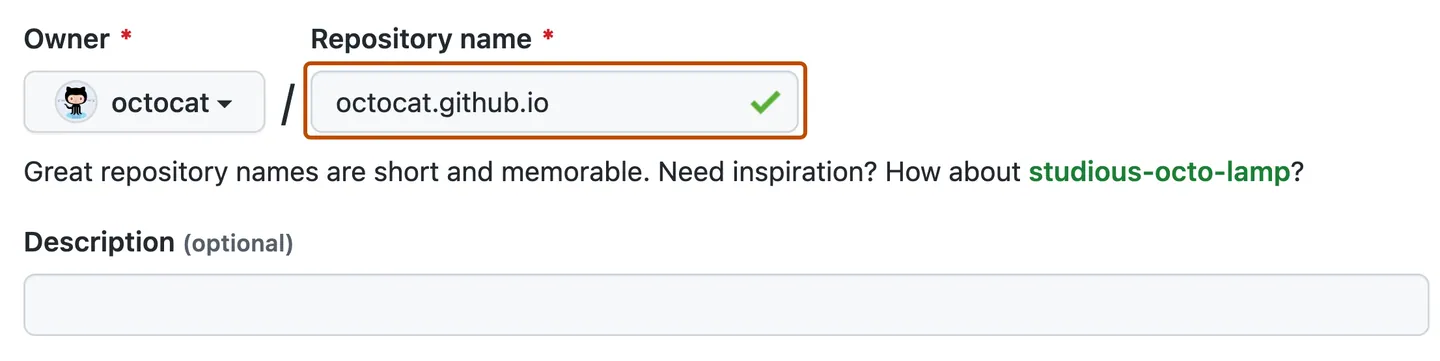
\includegraphics[keepaspectratio]{figures/repositorio.png}}

\begin{enumerate}
\def\labelenumi{\arabic{enumi}.}
\setcounter{enumi}{1}
\tightlist
\item
  Configura el repositorio como Público.
\item
  Agrega un README (opcional).
\item
  Haz clic en Create repository (Crear repositorio).
\item
  Posteriormente ir a \textbf{Settings} del repositorio \textgreater{}
  Pages. Y aquí encontraremos el URL de nuestro sitio web.
\end{enumerate}

\pandocbounded{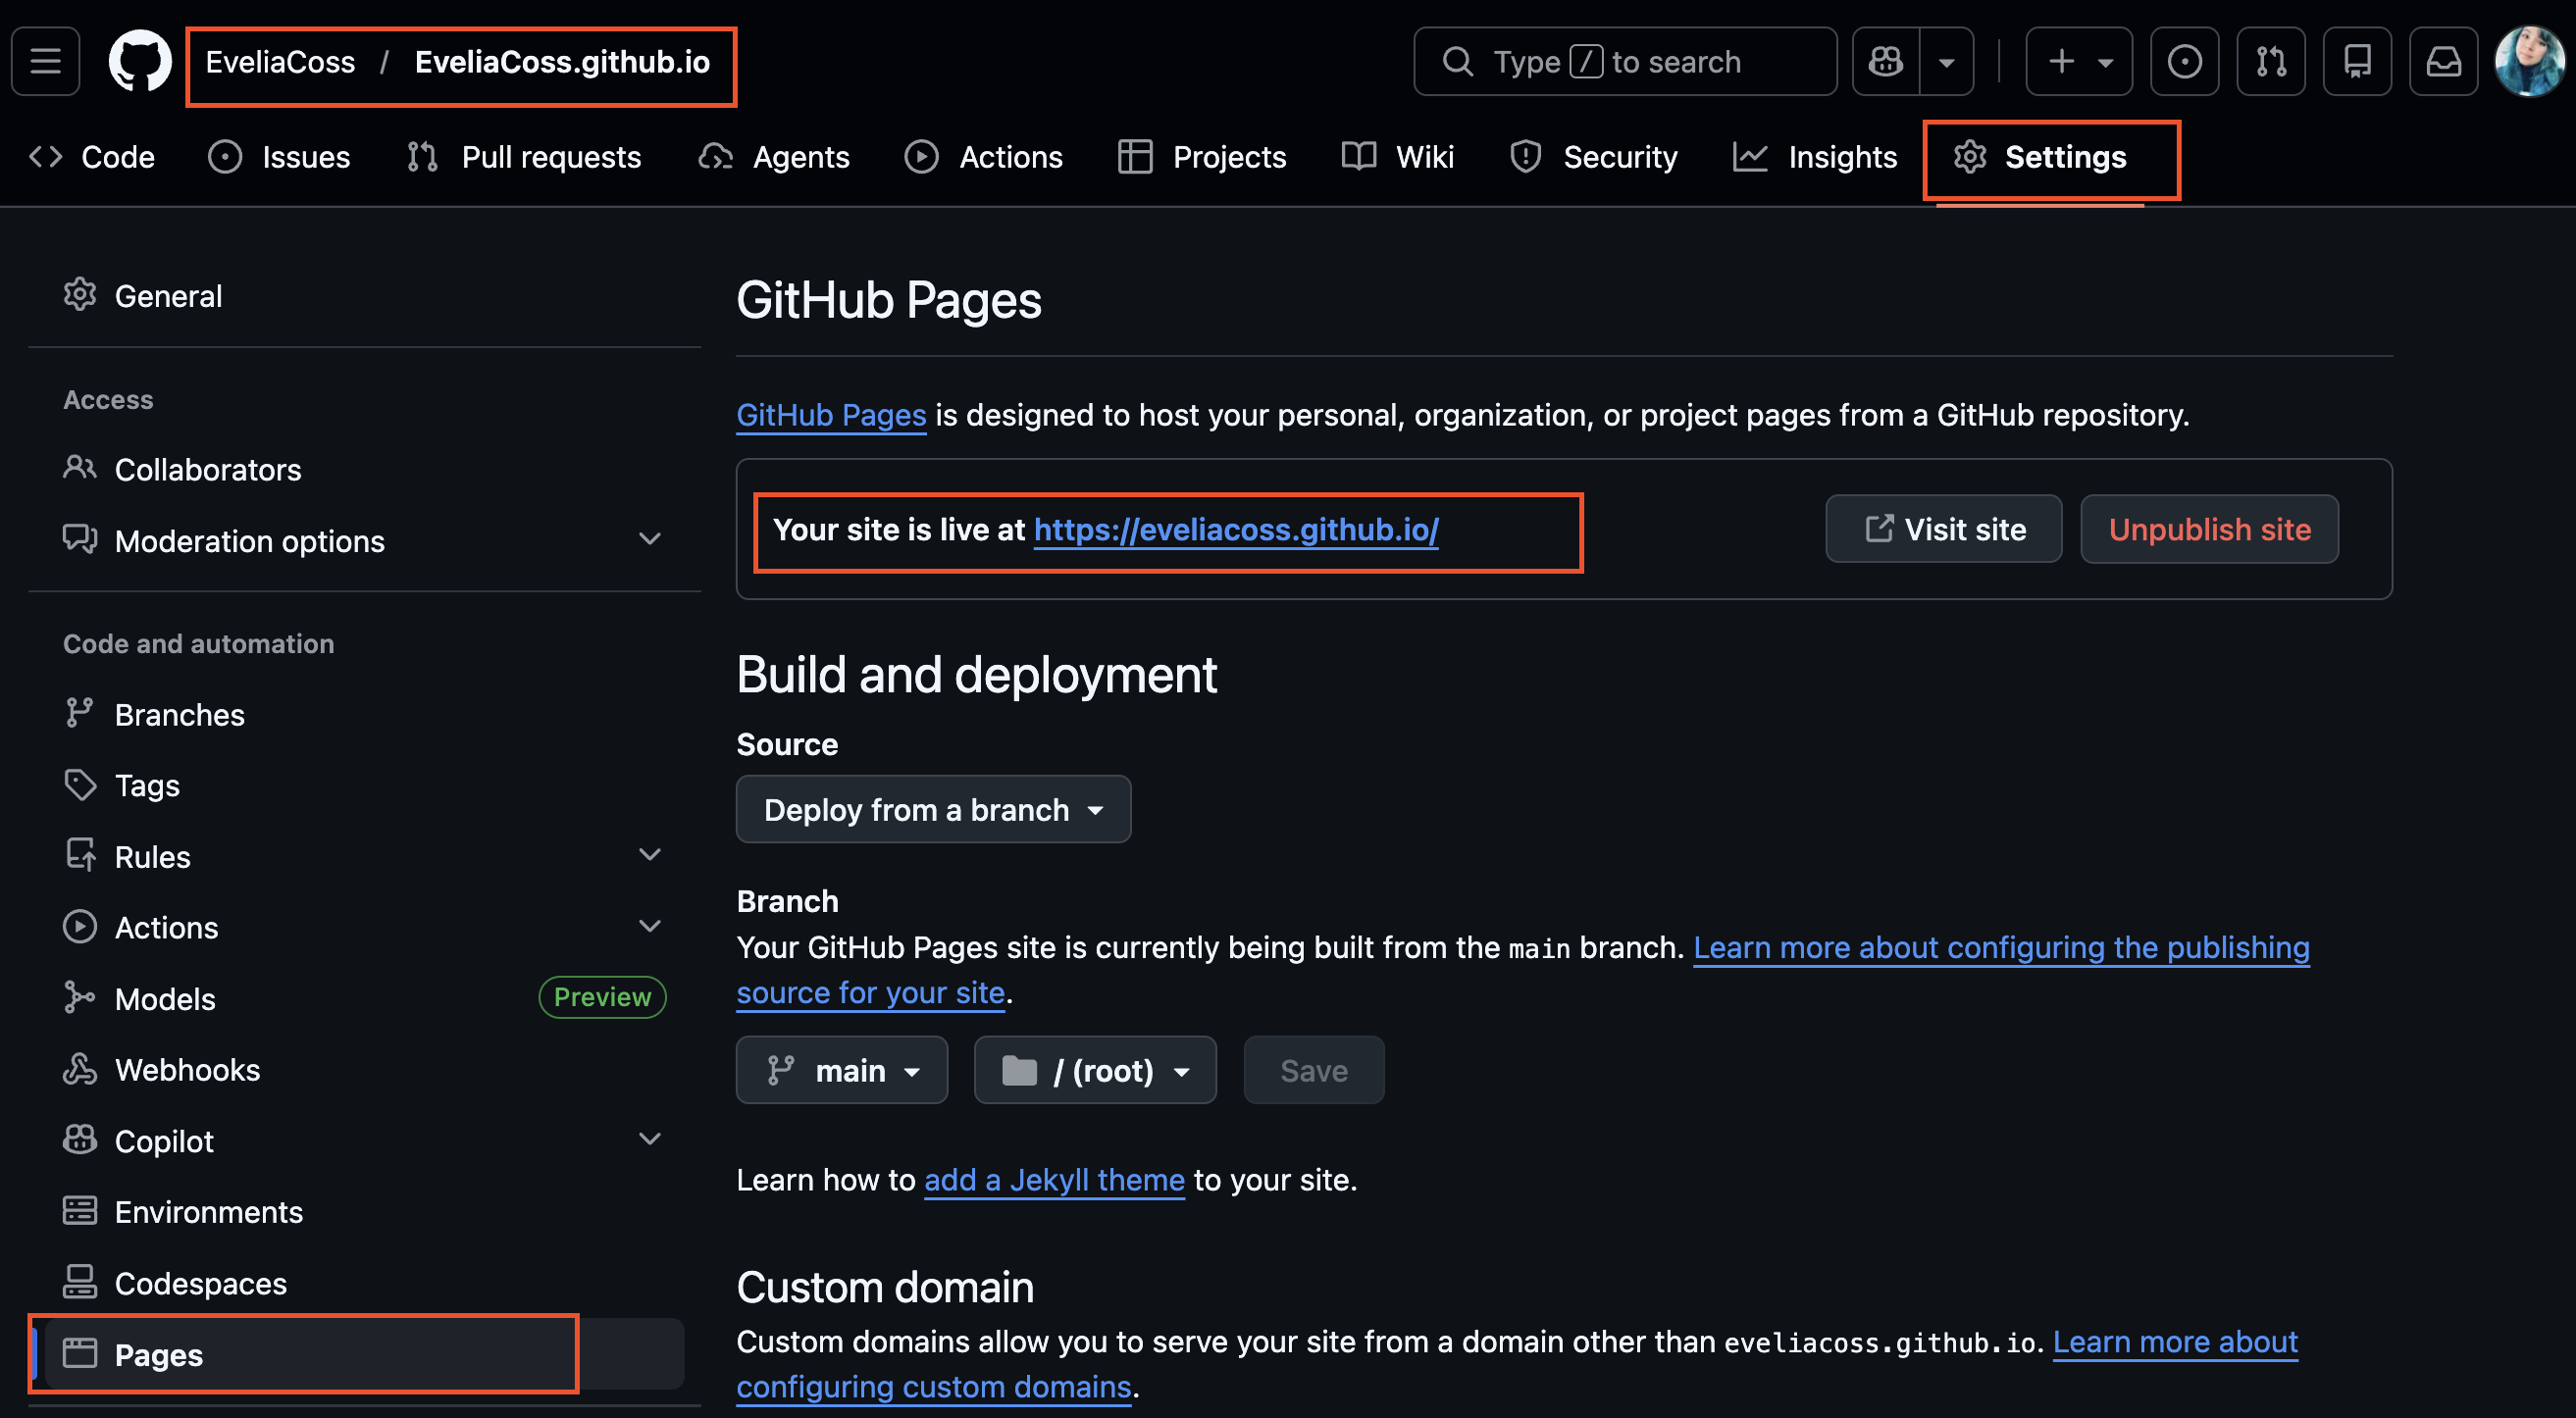
\includegraphics[keepaspectratio]{figures/EveliaCoss_webpages_config.png}}

\begin{tcolorbox}[enhanced jigsaw, arc=.35mm, bottomrule=.15mm, bottomtitle=1mm, breakable, colback=white, colbacktitle=quarto-callout-note-color!10!white, colframe=quarto-callout-note-color-frame, coltitle=black, left=2mm, leftrule=.75mm, opacityback=0, opacitybacktitle=0.6, rightrule=.15mm, title=\textcolor{quarto-callout-note-color}{\faInfo}\hspace{0.5em}{Nota}, titlerule=0mm, toprule=.15mm, toptitle=1mm]

En este punto de la clase debemos tener \textbf{dos repositorios} con
los siguientes nombres:

\begin{itemize}
\tightlist
\item
  \textbf{EveliaCoss/EveliaCoss}: Que va a contener el README de inicio
  de nuestro perfil.
\item
  \textbf{EveliaCoss/EveliaCoss.github.io}: Contendra nuestro dominio
  para los sitios web.
\end{itemize}

\pandocbounded{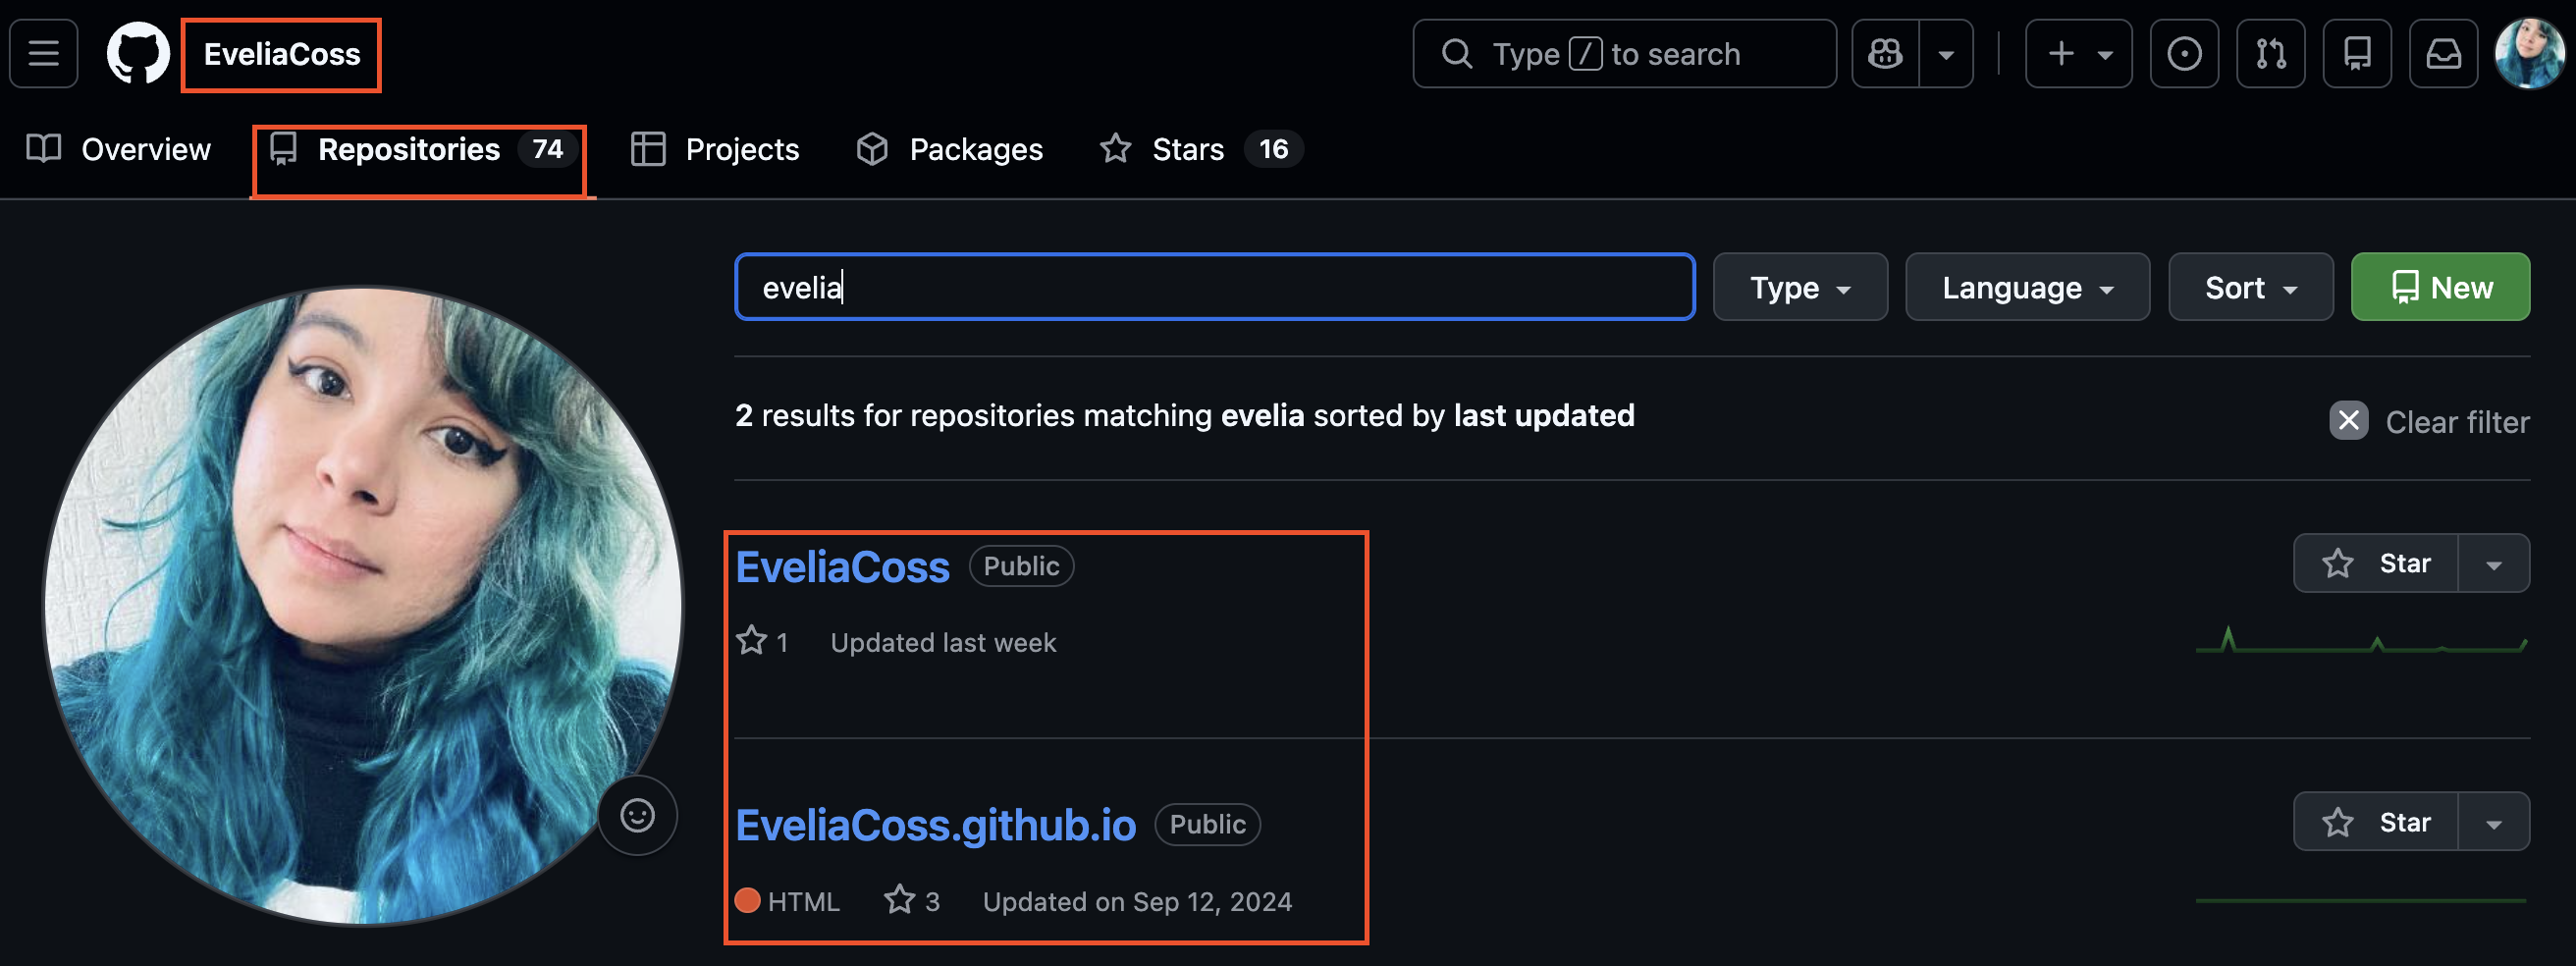
\includegraphics[keepaspectratio]{figures/EveliaCoss_repositorios.png}}

\end{tcolorbox}

\section{\texorpdfstring{\textbf{📌 Tareas}}{📌 Tareas}}\label{tareas}

Traer para la Próxima clase: \textbf{19 de febrero, 2026}, vamos a
\textbf{crear nuestra página web} empleando GitHub pages, por lo que
deben traer:

\begin{enumerate}
\def\labelenumi{\arabic{enumi}.}
\tightlist
\item
  Sincronizar su GitHub con Rstudio, revisar el material de
  \href{https://eveliacoss.github.io/Workshop_GitGithub2025/Parte1.html}{Conectar
  a GitHub con SSH}.
\item
  Traer una foto y su miniresumen para crear su página web con GitHub
  pages
\end{enumerate}

Ejemplo del Sitio Web que haremos en la siguiente clase:

\begin{center}
\pandocbounded{\includegraphics[keepaspectratio]{index_files/mediabag/9k=.jpg}}
\end{center}

\section{Referencias}\label{referencias-14}

\begin{itemize}
\tightlist
\item
  \href{https://docs.github.com/es/pages/getting-started-with-github-pages/creating-a-github-pages-site}{GitHub
  pages}
\item
  \href{https://rahuldkjain.github.io/gh-profile-readme-generator/}{GitHub
  Profile README Generator}
\end{itemize}

\chapter{Resumen y Práctica Final}\label{resumen-y-pruxe1ctica-final}

\section{Comandos usados en Github y
RStudio}\label{comandos-usados-en-github-y-rstudio}

\href{https://neurathsboat.blog/post/git-intro/}{\pandocbounded{\includegraphics[keepaspectratio]{index_files/mediabag/featured.png}}}

\begin{tcolorbox}[enhanced jigsaw, arc=.35mm, bottomrule=.15mm, bottomtitle=1mm, breakable, colback=white, colbacktitle=quarto-callout-important-color!10!white, colframe=quarto-callout-important-color-frame, coltitle=black, left=2mm, leftrule=.75mm, opacityback=0, opacitybacktitle=0.6, rightrule=.15mm, title=\textcolor{quarto-callout-important-color}{\faExclamation}\hspace{0.5em}{Importante}, titlerule=0mm, toprule=.15mm, toptitle=1mm]

\begin{itemize}
\item
  \texttt{git\ add:} Agregar cambios
\item
  \texttt{git\ status:} Revisamos el estado del proyecto
\item
  \texttt{git\ commit:} comentar los cambios
\item
  \texttt{git\ checkout:} Pordemos regresar cambios o cambiar de rama.
\end{itemize}

En Git, los comandos \texttt{git\ pull} y \texttt{git\ push} \textbf{son
utilizados para sincronizar y actualizar el contenido de un
repositorio}:~

\begin{itemize}
\item
  \texttt{git\ pull:} Actualiza la versión local de un repositorio desde
  otro remoto (en R studio flecha azul).
\item
  \texttt{git\ push:} Carga contenido en un repositorio remoto (en R
  studio flecha verde)
\end{itemize}

\end{tcolorbox}

\section{Página de inicio en
GitHub}\label{puxe1gina-de-inicio-en-github}

\begin{tcolorbox}[enhanced jigsaw, arc=.35mm, bottomrule=.15mm, bottomtitle=1mm, breakable, colback=white, colbacktitle=quarto-callout-note-color!10!white, colframe=quarto-callout-note-color-frame, coltitle=black, left=2mm, leftrule=.75mm, opacityback=0, opacitybacktitle=0.6, rightrule=.15mm, title=\textcolor{quarto-callout-note-color}{\faInfo}\hspace{0.5em}{Actividad}, titlerule=0mm, toprule=.15mm, toptitle=1mm]

\begin{enumerate}
\def\labelenumi{\arabic{enumi}.}
\tightlist
\item
  En GitHub, crea un repositorio con el mismo nombre de usuario.
  Ejemplo: Si el usuario es EveliaCoss y entonces el repositorio se
  llama EveliaCoss, dandonos la siguiente liga
  \url{https://github.com/EveliaCoss/EveliaCoss}
\item
  Agrega un README al repositorio con tu informacion. Por Default ya
  trae una plantilla, modificala y adaptala a tu gusto.
\item
  Visualiza como cambia tu inicio en el Github.
\end{enumerate}

Puedes aprender a realizar esta actividad paso a paso, siguiendo este
\href{https://eveliacoss.github.io/LCG2026_Buenas_practicas_presentacion_S4/Dia1_BuenasPracticas.html?panelset_002=repositorios-acad\%25C3\%25A9micos-y-cient\%25C3\%25ADficos2\#38}{tutorial}.

\end{tcolorbox}

\pandocbounded{
\includegraphics[keepaspectratio]{figures/EveliaCoss_inciio.jpg}}

\section{GitHub primero, RStudio
después\ldots{}}\label{github-primero-rstudio-despuuxe9s}

\begin{enumerate}
\def\labelenumi{\arabic{enumi}.}
\setcounter{enumi}{3}
\tightlist
\item
  En RStudio crea un nuevo proyecto: \emph{File} \textgreater{}
  \emph{New Project} \textgreater{} \emph{Version Control}
  \textgreater{} \emph{Git}. Ahi pega el URL del repositorio
  \texttt{https://github.com/mi\_usuario/mi\_repositorio.git}. Da click
  en \emph{Create Project}.
\end{enumerate}

Esto nos generará los siguientes elementos:

\begin{itemize}
\item
  Un directorio nuevo
\item
  Un repositorio Git enlazado a al repositorio de GitHub
\item
  Un proyecto en RStudio
\end{itemize}

Con este procedimiento ya no es necesario preocuparse por configurar
controles remotos Git y rastrear ramas en la línea de comandos.

\section{Comentar, pull y push en
Rstudio}\label{comentar-pull-y-push-en-rstudio}

\href{https://comunidadbioinfo.github.io/cdsb2023/control-de-versiones-con-github-y-rstudio.html}{\includegraphics[width=6.25in,height=\textheight,keepaspectratio]{index_files/mediabag/gitrstudio_comment.png}}

Con la \textbf{flecha azul} podemos hacer pull (\textbf{RECUERDA HACERLO
ANTES DE HACER UN PUSH}), y con la flecha verde un \texttt{push}. Para
poder comentar y hacer push debemos marcar con una palomita mediante un
\texttt{click} en las pequeñas cajas blancas de la columna
\emph{Staged}, damos click en \emph{commit} lo cual nos abre la
siguiente ventana.

\pandocbounded{\includegraphics[keepaspectratio]{index_files/mediabag/gitrstudio_push.png}}

Volvemos a dar \texttt{click} en \emph{commit}, y finalizamos con
\emph{push} (flecha verde).

\section{Ediciones desde R de la página de inicio en
GitHub}\label{ediciones-desde-r-de-la-puxe1gina-de-inicio-en-github}

\begin{tcolorbox}[enhanced jigsaw, arc=.35mm, bottomrule=.15mm, bottomtitle=1mm, breakable, colback=white, colbacktitle=quarto-callout-note-color!10!white, colframe=quarto-callout-note-color-frame, coltitle=black, left=2mm, leftrule=.75mm, opacityback=0, opacitybacktitle=0.6, rightrule=.15mm, title=\textcolor{quarto-callout-note-color}{\faInfo}\hspace{0.5em}{Actividad}, titlerule=0mm, toprule=.15mm, toptitle=1mm]

\begin{enumerate}
\def\labelenumi{\arabic{enumi}.}
\tightlist
\item
  Sincroniza el repositorio con el nombre de tu usuario en GitHub
  (ejemplo:
  \href{https://github.com/EveliaCoss/EveliaCoss}{EveliaCoss/EveliaCoss})
  con RStudio
\item
  Realiza los cambios desde R y subelos a GitHub.
\item
  Visualiza como cambia tu inicio en el Github.
\end{enumerate}

\end{tcolorbox}

\begin{tcolorbox}[enhanced jigsaw, arc=.35mm, bottomrule=.15mm, bottomtitle=1mm, breakable, colback=white, colbacktitle=quarto-callout-tip-color!10!white, colframe=quarto-callout-tip-color-frame, coltitle=black, left=2mm, leftrule=.75mm, opacityback=0, opacitybacktitle=0.6, rightrule=.15mm, title=\textcolor{quarto-callout-tip-color}{\faLightbulb}\hspace{0.5em}{Oh Shit, Git!?!}, titlerule=0mm, toprule=.15mm, toptitle=1mm]

También existe esta página llamada \href{https://ohshitgit.com/}{Oh
Shit, Git!?!}. En donde puedes aprender sobre los errores comunes en
GitHub.

\end{tcolorbox}

\pandocbounded{
\includegraphics[keepaspectratio]{figures/github_mergeconflic.png}}

Imagen tomada de \href{https://allisonhorst.com/git-github}{Allison
Horst.}

\section{Referencias}\label{referencias-15}

\begin{itemize}
\tightlist
\item
  Evelia
  tutorial:\href{https://eveliacoss.github.io/Workshop_GitGithub2025/}{Workshop
  sobre Git / Github 2025}
\item
  Haydee tutorial:
  \href{https://haydeeperuyero.github.io/Computo_Cientifico/}{Temas
  Selectos de Análisis Numérico y Computación Científica: Computo
  científico para el análisis de datos}
\item
  Alejandra Medina tutorial:
  \href{https://comunidadbioinfo.github.io/cdsb2023/control-de-versiones-con-github-y-rstudio.html}{Control
  de versiones con GitHub y RStudio}
\end{itemize}

\part{\textbf{Sección 6} - Introducción a R y Rstudio}

\chapter{Introducción a Markdown}\label{introducciuxf3n-a-markdown}

\section{¿Qué es Markdown?}\label{quuxe9-es-markdown}

Markdown es un \textbf{lenguaje de marcado ligero} que permite añadir
elementos de formato a documentos de \emph{texto plano}. Creado por John
Gruber en 2004, Markdown es actualmente uno de los lenguajes más
populares del mundo.

\begin{itemize}
\tightlist
\item
  Sencillo y legible, sin necesidad de usar editores complicados o HTML.
\item
  \textbf{lenguaje de marcado ligero:} Escribir texto que incluye
  instrucciones simples para darle formato.
\end{itemize}

\begin{tcolorbox}[enhanced jigsaw, arc=.35mm, bottomrule=.15mm, bottomtitle=1mm, breakable, colback=white, colbacktitle=quarto-callout-note-color!10!white, colframe=quarto-callout-note-color-frame, coltitle=black, left=2mm, leftrule=.75mm, opacityback=0, opacitybacktitle=0.6, rightrule=.15mm, title=\textcolor{quarto-callout-note-color}{\faInfo}\hspace{0.5em}{🧩 ¿Por qué se llama ``ligero''?}, titlerule=0mm, toprule=.15mm, toptitle=1mm]

Porque:

\begin{itemize}
\tightlist
\item
  Usa símbolos sencillos como \texttt{*,\ \#,} o \texttt{-} para indicar
  formato.
\item
  No requiere cerrar etiquetas como
  \texttt{\textless{}strong\textgreater{}\ o\ \textless{}div\textgreater{}}
  (como en HTML).
\item
  Es minimalista y limpio, ideal para escribir rápido sin distracciones.
\end{itemize}

\end{tcolorbox}

\section{🧠 ¿Para qué se usa?}\label{para-quuxe9-se-usa}

\begin{itemize}
\tightlist
\item
  Crear documentación técnica o científica
\item
  Escribir \textbf{README.md} en proyectos de GitHub
\item
  Generar contenido para sitios web
\item
  Crear
  \href{https://quarto.org/docs/get-started/hello/rstudio.html}{tesis},
  notas, \href{https://bookdown.org/yihui/rmarkdown-cookbook/}{libros},
  \href{https://bookdown.org/yihui/rmarkdown/xaringan.html}{presentaciones}
  y posters
\end{itemize}

\textbf{En R}

{\def\LTcaptype{none} % do not increment counter
\begin{longtable}[]{@{}
  >{\raggedright\arraybackslash}p{(\linewidth - 2\tabcolsep) * \real{0.5000}}
  >{\raggedright\arraybackslash}p{(\linewidth - 2\tabcolsep) * \real{0.5000}}@{}}
\toprule\noalign{}
\begin{minipage}[b]{\linewidth}\raggedright
Paquete / Programa
\end{minipage} & \begin{minipage}[b]{\linewidth}\raggedright
Uso principal
\end{minipage} \\
\midrule\noalign{}
\endhead
\bottomrule\noalign{}
\endlastfoot
\href{https://github.com/EveliaCoss/RmarkdownGraphs_notes}{\texttt{rmarkdown}}
& Crear documentos reproducibles con texto, código y resultados \\
\texttt{knitr} & Ejecutar chunks de código en RMarkdown \\
\href{https://quarto.org/docs/get-started/hello/vscode.html}{\texttt{Quarto}}
& Plataforma moderna para documentos con R, Python, etc. \\
\texttt{bookdown} & Crear libros técnicos con Markdown + RMarkdown \\
\texttt{blogdown} & Generar blogs científicos usando Markdown y Hugo \\
\texttt{flexdashboard} & Dashboards interactivos escritos en Markdown \\
\end{longtable}
}

\textbf{En Python}

{\def\LTcaptype{none} % do not increment counter
\begin{longtable}[]{@{}
  >{\raggedright\arraybackslash}p{(\linewidth - 2\tabcolsep) * \real{0.5000}}
  >{\raggedright\arraybackslash}p{(\linewidth - 2\tabcolsep) * \real{0.5000}}@{}}
\toprule\noalign{}
\begin{minipage}[b]{\linewidth}\raggedright
Paquete / Programa
\end{minipage} & \begin{minipage}[b]{\linewidth}\raggedright
Uso principal
\end{minipage} \\
\midrule\noalign{}
\endhead
\bottomrule\noalign{}
\endlastfoot
Jupyter Notebooks & Celdas Markdown para explicar y documentar junto con
código \\
\texttt{Quarto} & Igual que en R, permite combinar Markdown con código
Python \\
\texttt{mkdocs} & Generar sitios web de documentación técnica desde
archivos Markdown \\
\texttt{Sphinx\ +\ MyST} & Documentación avanzada con soporte para
Markdown \\
\texttt{markdown}, \texttt{mistune} & Librerías para convertir Markdown
a HTML \\
\texttt{nbconvert} & Exportar notebooks con Markdown a PDF, HTML, LaTeX,
etc. \\
\end{longtable}
}

\section{¿Cómo funciona?}\label{cuxf3mo-funciona-1}

Pasos generales:

\begin{enumerate}
\def\labelenumi{\arabic{enumi}.}
\tightlist
\item
  Crear un archivo Markdown con un editor de texto o una aplicación
  específica. El archivo debe tener la extensión
  \texttt{.md\ o\ .markdown}.
\item
  Se abre el archivo Markdown en una aplicación Markdown.
\item
  Se utiliza la aplicación Markdown para convertir el archivo Markdown
  en un documento HTML.
\item
  Visualización del archivo HTML en un navegador web o use la aplicación
  Markdown para convertirlo a otro formato de archivo, como PDF.
\end{enumerate}

\begin{tcolorbox}[enhanced jigsaw, arc=.35mm, bottomrule=.15mm, bottomtitle=1mm, breakable, colback=white, colbacktitle=quarto-callout-note-color!10!white, colframe=quarto-callout-note-color-frame, coltitle=black, left=2mm, leftrule=.75mm, opacityback=0, opacitybacktitle=0.6, rightrule=.15mm, title=\textcolor{quarto-callout-note-color}{\faInfo}\hspace{0.5em}{Nota}, titlerule=0mm, toprule=.15mm, toptitle=1mm]

La aplicación y el procesador de Markdown son dos componentes
independientes. Para simplificar, los he combinado en un solo elemento
(``aplicación de Markdown'') en la figura a continuación.

\end{tcolorbox}

\begin{figure}[H]

{\centering \pandocbounded{\includegraphics[keepaspectratio]{reproducible/figures/markdown-flowchart.png}}

}

\caption{Imagen tomada de:
https://www.markdownguide.org/getting-started/}

\end{figure}%

\section{\texorpdfstring{\textbf{Sintaxis de escritura y formato
básicos}}{Sintaxis de escritura y formato básicos}}\label{sintaxis-de-escritura-y-formato-buxe1sicos}

Revisar la
\href{https://docs.github.com/es/get-started/writing-on-github/getting-started-with-writing-and-formatting-on-github/basic-writing-and-formatting-syntax}{documentación
de GitHub}

\section{Tablas con datatable}\label{tablas-con-datatable}

\begin{Shaded}
\begin{Highlighting}[]
\FunctionTok{library}\NormalTok{(dplyr)}

\NormalTok{iris }\SpecialCharTok{\%\textgreater{}\%}
  \FunctionTok{head}\NormalTok{(}\DecValTok{3}\NormalTok{) }\SpecialCharTok{\%\textgreater{}\%}
\NormalTok{  DT}\SpecialCharTok{::}\FunctionTok{datatable}\NormalTok{()}
\end{Highlighting}
\end{Shaded}

\begin{table}

\caption{\label{tbl-bonita}Tabla decorativa}

\centering{

\pandocbounded{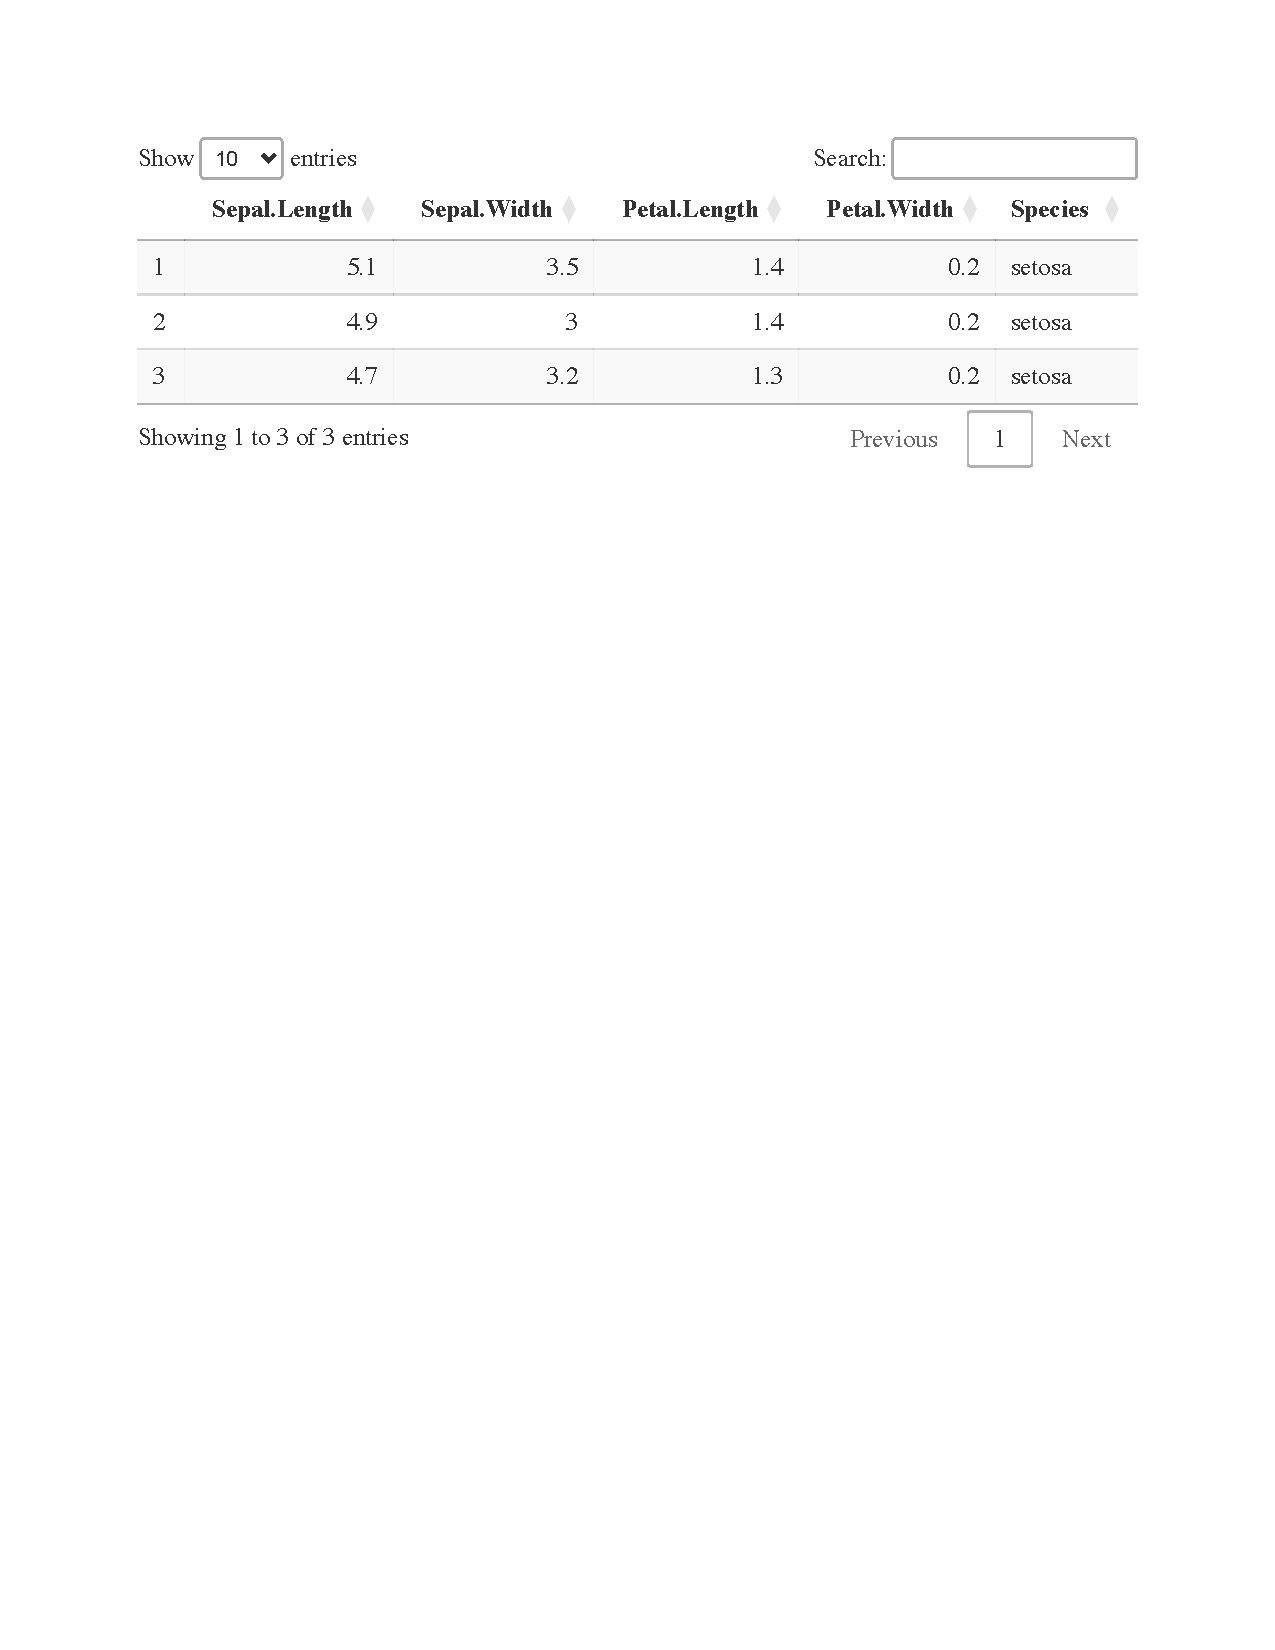
\includegraphics[keepaspectratio]{cap29_files/figure-pdf/tbl-bonita-1.pdf}}

}

\end{table}%

\section{\texorpdfstring{\href{https://gt.rstudio.com/index.html}{\texttt{library(gt)}}}{library(gt)}}\label{librarygt}

\begin{Shaded}
\begin{Highlighting}[]
\NormalTok{iris }\SpecialCharTok{\%\textgreater{}\%} 
  \FunctionTok{head}\NormalTok{() }\SpecialCharTok{\%\textgreater{}\%}
\NormalTok{  gt}\SpecialCharTok{::}\FunctionTok{gt}\NormalTok{() }\SpecialCharTok{\%\textgreater{}\%}
\NormalTok{  gt}\SpecialCharTok{::}\FunctionTok{tab\_spanner}\NormalTok{(}\AttributeTok{label =} \StringTok{"Petalo"}\NormalTok{, }\AttributeTok{columns =} \FunctionTok{vars}\NormalTok{(Petal.Length,Petal.Width)) }\SpecialCharTok{\%\textgreater{}\%}
\NormalTok{  gt}\SpecialCharTok{::}\FunctionTok{tab\_spanner}\NormalTok{(}\AttributeTok{label =} \StringTok{"Sepalo"}\NormalTok{, }\AttributeTok{columns =} \FunctionTok{vars}\NormalTok{(Sepal.Length,Sepal.Width))}
\end{Highlighting}
\end{Shaded}

\begin{table}
\fontsize{12.0pt}{14.0pt}\selectfont
\begin{tabular*}{\linewidth}{@{\extracolsep{\fill}}rrrrc}
\toprule
\multicolumn{2}{c}{{Sepalo}} & \multicolumn{2}{c}{{Petalo}} &  \\ 
\cmidrule(lr){1-2} \cmidrule(lr){3-4}
Sepal.Length & Sepal.Width & Petal.Length & Petal.Width & Species \\ 
\midrule\addlinespace[2.5pt]
5.1 & 3.5 & 1.4 & 0.2 & setosa \\ 
4.9 & 3.0 & 1.4 & 0.2 & setosa \\ 
4.7 & 3.2 & 1.3 & 0.2 & setosa \\ 
4.6 & 3.1 & 1.5 & 0.2 & setosa \\ 
5.0 & 3.6 & 1.4 & 0.2 & setosa \\ 
5.4 & 3.9 & 1.7 & 0.4 & setosa \\ 
\bottomrule
\end{tabular*}
\end{table}

\begin{tcolorbox}[enhanced jigsaw, arc=.35mm, bottomrule=.15mm, bottomtitle=1mm, breakable, colback=white, colbacktitle=quarto-callout-note-color!10!white, colframe=quarto-callout-note-color-frame, coltitle=black, left=2mm, leftrule=.75mm, opacityback=0, opacitybacktitle=0.6, rightrule=.15mm, title=\textcolor{quarto-callout-note-color}{\faInfo}\hspace{0.5em}{Nota}, titlerule=0mm, toprule=.15mm, toptitle=1mm]

Si gustas repasar podemos hacerlo con el script
\href{https://github.com/EveliaCoss/RmarkdownGraphs_notes/blob/main/Sesion_Rmarkdown_13Oct2023.Rmd}{Sesion\_Rmarkdown\_13Oct2023.Rmd}
del repositorio
\href{https://github.com/EveliaCoss/RmarkdownGraphs_notes/tree/main}{RmarkdownGraphs\_notes}\textbf{.}

\end{tcolorbox}

\section{Referencias}\label{referencias-16}

\begin{itemize}
\tightlist
\item
  \href{https://docs.github.com/es/get-started/writing-on-github/getting-started-with-writing-and-formatting-on-github/basic-writing-and-formatting-syntax}{Documentación
  de GitHub}
\item
  \href{https://michael-franke.github.io/intro-data-analysis/ch-01-01-Rmarkdown.html}{Libro
  de Rmarkdown}
\item
  \href{https://www.markdowntutorial.com/es/lesson/1/}{Ejercicios con
  Markdown}
\item
  \href{https://lcg-cursos.github.io/material/introbioinfo/}{Curso de
  Heladia Salgado}
\item
  Curso de
  \href{https://eveliacoss.github.io/Workshop_GitGithub2025/Parte2.html}{Git
  y GitHub Evelia Coss}
\item
  \href{https://faculty.washington.edu/otoomet/info201-book/markdown.html}{Markdown
  and rmarkdown}
\item
  \href{https://rmarkdown.rstudio.com/gallery.html}{Galeria de Markdown}
\item
  \href{https://zsmith27.github.io/rmarkdown_crash-course/lesson-3-basic-syntax.html}{Lesson
  3: Basic Syntax}
\item
  \href{https://carpentries-incubator.github.io/open-science-with-r/aio/index.html}{Introduction
  to Open Data Science with R}
\item
  \href{https://bookdown.org/hneth/ds4psy/}{Data Science for
  Psychologists}
\end{itemize}

\chapter{\texorpdfstring{\textbf{📚} Actividad 3: Página web con
Rmarkdown}{📚 Actividad 3: Página web con Rmarkdown}}\label{actividad-3-puxe1gina-web-con-rmarkdown}

\textbf{Fecha:} 19 de febrero, 2026

\begin{center}
\pandocbounded{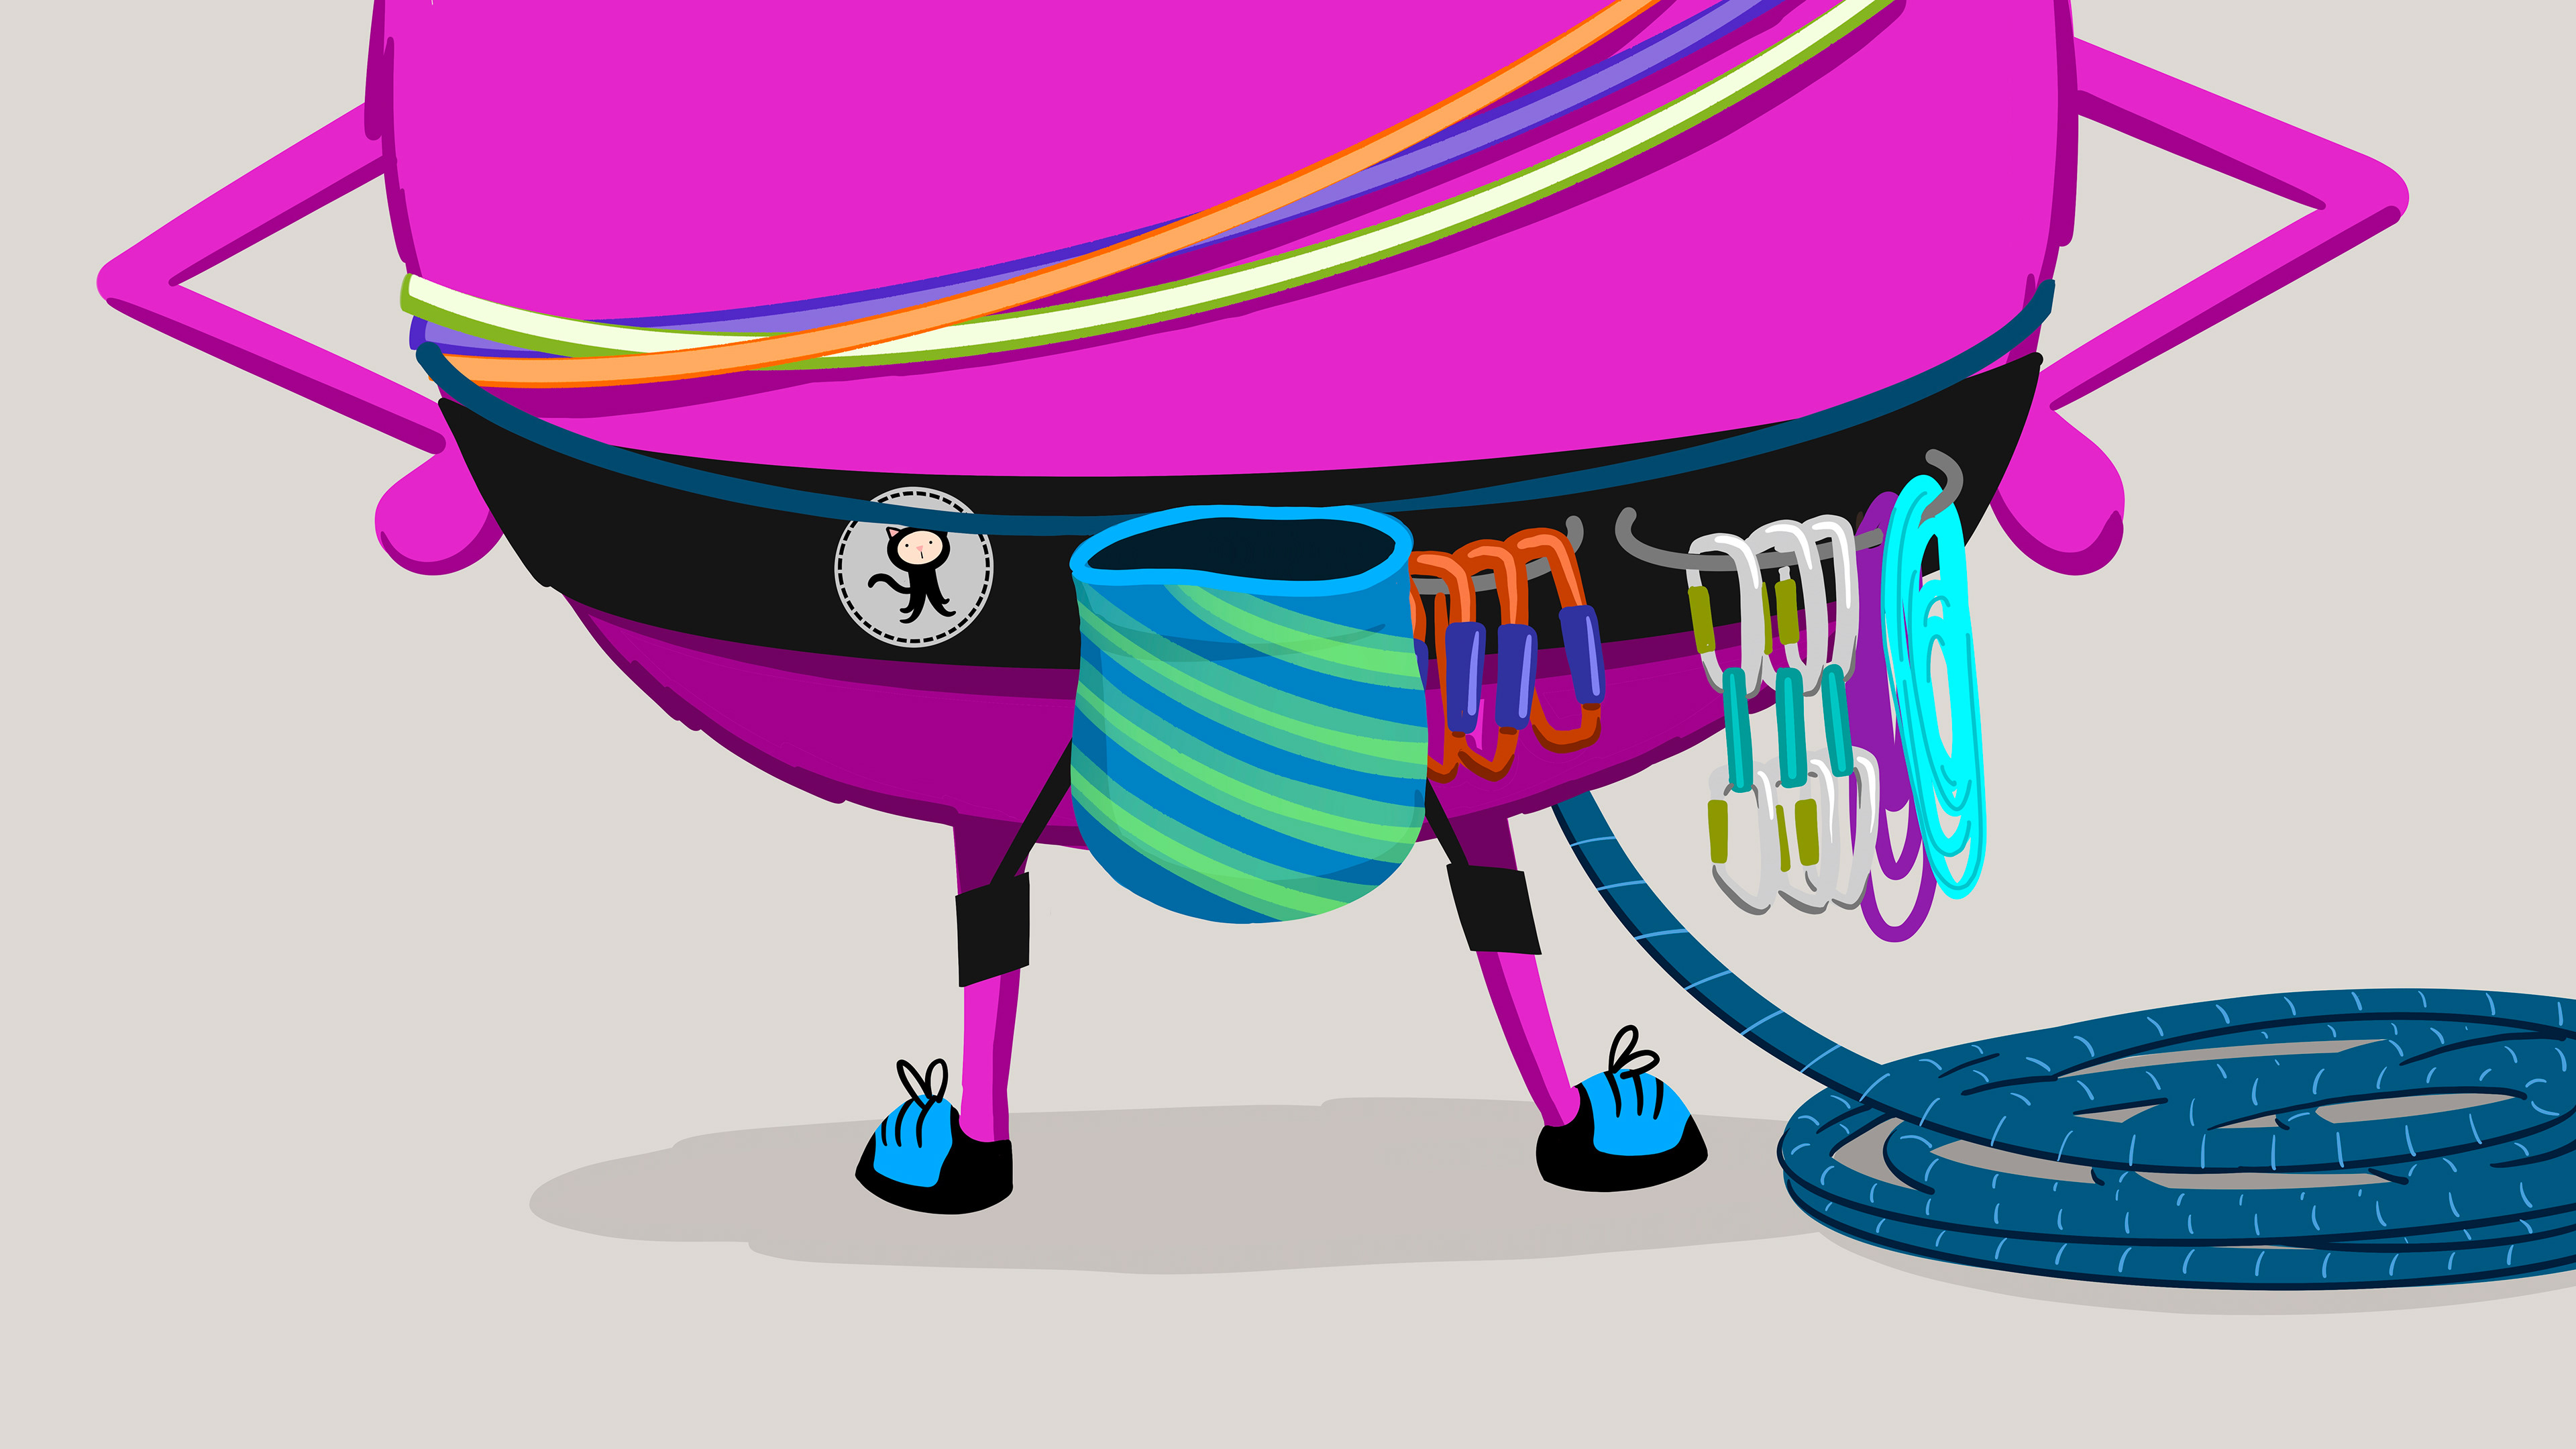
\includegraphics[keepaspectratio]{figures/clipboard-1640307360.png}}
\end{center}

Imagen tomada de: \href{https://allisonhorst.com/git-github}{Allison
Horst}

\subsection{¿Qué es un RProject y por qué
usarlo?}\label{quuxe9-es-un-rproject-y-por-quuxe9-usarlo}

\begin{itemize}
\item
  \textbf{Carpeta de trabajo dedicada}: al crear un RProject, RStudio
  genera automáticamente una carpeta que contiene todos los archivos y
  configuraciones necesarias para tu proyecto.
\item
  \textbf{Organización}: te permite mantener en un solo lugar tus
  scripts, datos, variables y documentos relacionados.
\item
  \textbf{Reproducibilidad}: facilita que cualquier persona (incluido tú
  en el futuro) pueda abrir el proyecto y trabajar con el mismo entorno.
\item
  \textbf{Integración con Git/GitHub}: al tener el mismo nombre que tu
  repositorio, se asegura una sincronización más clara y ordenada entre
  tu proyecto local y el repositorio remoto.
\end{itemize}

\pandocbounded{
\includegraphics[keepaspectratio]{figures/clipboard-3718600223.png}}

Imagen tomada de: \href{https://allisonhorst.com/git-github}{Allison
Horst}

\chapter{\texorpdfstring{\textbf{📚} Actividades 3A, 3B y
3C}{📚 Actividades 3A, 3B y 3C}}\label{actividades-3a-3b-y-3c}

\href{https://allisonhorst.com/horst-hill-collaborations}{\pandocbounded{\includegraphics[keepaspectratio]{figures/clipboard-302116819.png}}}

Imagen tomada de:
\href{https://allisonhorst.com/horst-hill-collaborations}{Allison Horst}

\begin{tcolorbox}[enhanced jigsaw, arc=.35mm, bottomrule=.15mm, bottomtitle=1mm, breakable, colback=white, colbacktitle=quarto-callout-note-color!10!white, colframe=quarto-callout-note-color-frame, coltitle=black, left=2mm, leftrule=.75mm, opacityback=0, opacitybacktitle=0.6, rightrule=.15mm, title=\textcolor{quarto-callout-note-color}{\faInfo}\hspace{0.5em}{📕 Actividad 3A: Crear un Rproject para el repositorio de GitHub}, titlerule=0mm, toprule=.15mm, toptitle=1mm]

\begin{enumerate}
\def\labelenumi{\arabic{enumi}.}
\tightlist
\item
  Da clic en \textbf{File/New project.}
\item
  Coloca el mismo nombre del repositorio que creamos en GitHub, debe
  llamadarse \textbf{usuario.github.io,} en mi ejemplo sería:
  \textbf{EveliaCoss.github.io.}
\item
  Checar que tengamos una carpeta con este nombre y un Rproject como el
  que se muestra acontinuación.
\end{enumerate}

\end{tcolorbox}

\begin{center}

\includegraphics[width=2.63542in,height=\textheight,keepaspectratio]{figures/clipboard-1393911157.png}
\end{center}

\begin{tcolorbox}[enhanced jigsaw, arc=.35mm, bottomrule=.15mm, bottomtitle=1mm, breakable, colback=white, colbacktitle=quarto-callout-note-color!10!white, colframe=quarto-callout-note-color-frame, coltitle=black, left=2mm, leftrule=.75mm, opacityback=0, opacitybacktitle=0.6, rightrule=.15mm, title=\textcolor{quarto-callout-note-color}{\faInfo}\hspace{0.5em}{📗 Actividad 3B: Obtener plantilla para la página web}, titlerule=0mm, toprule=.15mm, toptitle=1mm]

\begin{enumerate}
\def\labelenumi{\arabic{enumi}.}
\tightlist
\item
  Descarga el archivo
  \href{https://github.com/EveliaCoss/EveliaCoss.github.io/blob/main/index.Rmd}{index.Rmd}
  de mi GitHub, y colocalo dentro de la misma carpeta que dice
  \textbf{usuario.github.io}.
\item
  Abre el \texttt{.Rproj.}
\item
  Abre el archivo
  \href{https://github.com/EveliaCoss/EveliaCoss.github.io/blob/main/index.Rmd}{index.Rmd}
  dentro de tu Rproject.
\end{enumerate}

\end{tcolorbox}

\begin{tcolorbox}[enhanced jigsaw, arc=.35mm, bottomrule=.15mm, bottomtitle=1mm, breakable, colback=white, colbacktitle=quarto-callout-note-color!10!white, colframe=quarto-callout-note-color-frame, coltitle=black, left=2mm, leftrule=.75mm, opacityback=0, opacitybacktitle=0.6, rightrule=.15mm, title=\textcolor{quarto-callout-note-color}{\faInfo}\hspace{0.5em}{📘 Actividad 3C: Vincular tu RProject con el repositorio de GitHub}, titlerule=0mm, toprule=.15mm, toptitle=1mm]

\begin{enumerate}
\def\labelenumi{\arabic{enumi}.}
\tightlist
\item
  Inicializa Git en tu Rproject desde la \textbf{terminal}.
\end{enumerate}

\begin{Shaded}
\begin{Highlighting}[]
\FunctionTok{git}\NormalTok{ init}
\end{Highlighting}
\end{Shaded}

\begin{enumerate}
\def\labelenumi{\arabic{enumi}.}
\setcounter{enumi}{1}
\tightlist
\item
  Conectar con GitHub. Reemplaza \texttt{usuario/nombre-repo} con tu
  repositorio real.
\end{enumerate}

\begin{Shaded}
\begin{Highlighting}[]
\FunctionTok{git}\NormalTok{ remote add origin https://github.com/usuario/nombre{-}repo.git}
\end{Highlighting}
\end{Shaded}

El link puedes obtenerlo dando clic en el código verde que dice
\textbf{CODE \textgreater{} HTTPS \textgreater{} copiar}.

\pandocbounded{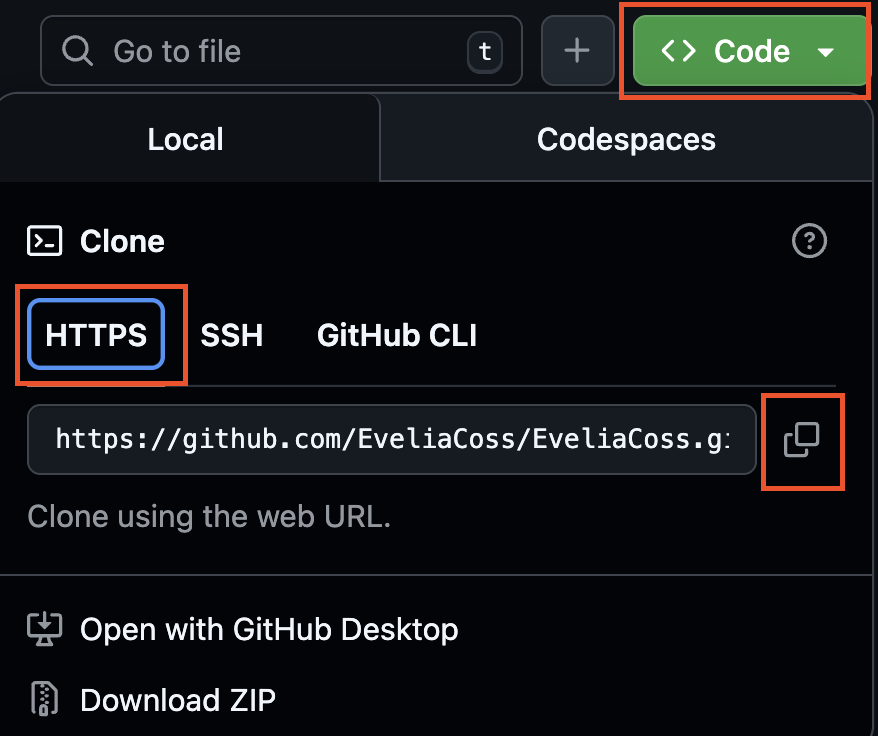
\includegraphics[keepaspectratio]{figures/clipboard-527850784.png}}

\begin{enumerate}
\def\labelenumi{\arabic{enumi}.}
\setcounter{enumi}{2}
\tightlist
\item
  Realiza el primer commit, agregando toda la información de la Rproject
\end{enumerate}

\begin{verbatim}
git add .
git commit -m "Primer commit"
git push -u origin main
\end{verbatim}

\begin{enumerate}
\def\labelenumi{\arabic{enumi}.}
\setcounter{enumi}{3}
\tightlist
\item
  Verifica los cambios en el GitHub. Después de hacer \emph{push}, tu
  proyecto debería aparecer en GitHub con todos los archivos.
\end{enumerate}

\end{tcolorbox}

\section{Otra manera de realizar commits en
R}\label{otra-manera-de-realizar-commits-en-r}

Cuando vinculas tu proyecto de R (\texttt{.Rproj}) con GitHub y
habilitas Git, aparece una nueva pestaña llamada \textbf{Git} en la
parte superior derecha de RStudio. Desde ahí puedes manejar tus cambios
sin necesidad de usar la terminal.

\pandocbounded{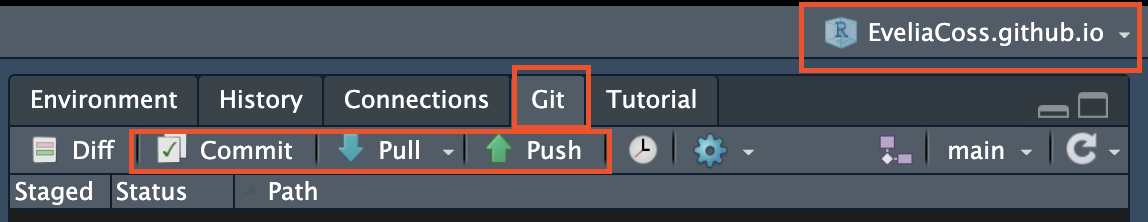
\includegraphics[keepaspectratio]{figures/clipboard-4087314388.png}}

\subsection{Flujo típico de trabajo}\label{flujo-tuxedpico-de-trabajo}

\begin{enumerate}
\def\labelenumi{\arabic{enumi}.}
\item
  \textbf{Detectar cambios}

  \begin{itemize}
  \tightlist
  \item
    Cada vez que modificas un archivo, RStudio lo marca en la pestaña
    \emph{Git}.
  \item
    Verás íconos que indican si el archivo fue \textbf{modificado (M),
    agregado (A) o eliminado (D)}.
  \end{itemize}
\end{enumerate}

\pandocbounded{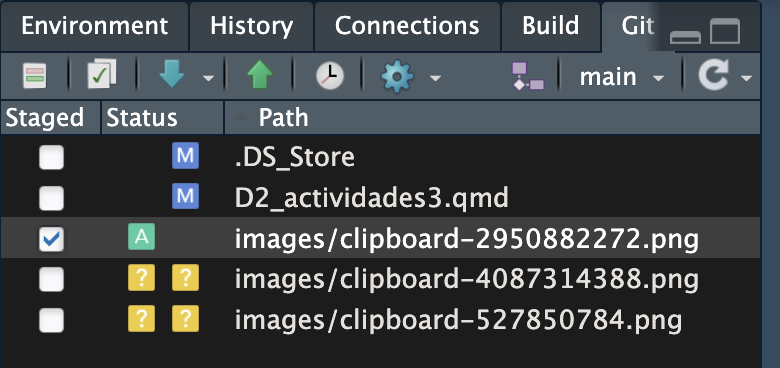
\includegraphics[keepaspectratio]{figures/clipboard-1204937639.png}}

\begin{enumerate}
\def\labelenumi{\arabic{enumi}.}
\setcounter{enumi}{1}
\item
  \textbf{Seleccionar archivos para el commit}

  \begin{itemize}
  \tightlist
  \item
    Marca las casillas de los archivos que quieres incluir en el commit.
  \item
    Esto equivale a \texttt{git\ add} en la terminal.
  \end{itemize}
\item
  \textbf{Escribir el mensaje de commit}

  \begin{itemize}
  \tightlist
  \item
    En el cuadro de texto escribe un mensaje claro y descriptivo, por
    ejemplo: \emph{``Corrijo error en función de normalización''}
  \item
    El mensaje debe explicar \textbf{qué cambiaste y por qué}.
  \end{itemize}
\item
  \textbf{Hacer el commit}

  \begin{itemize}
  \tightlist
  \item
    Haz clic en el botón \emph{Commit}.
  \item
    Esto guarda los cambios en tu historial local de Git.
  \end{itemize}
\end{enumerate}

\pandocbounded{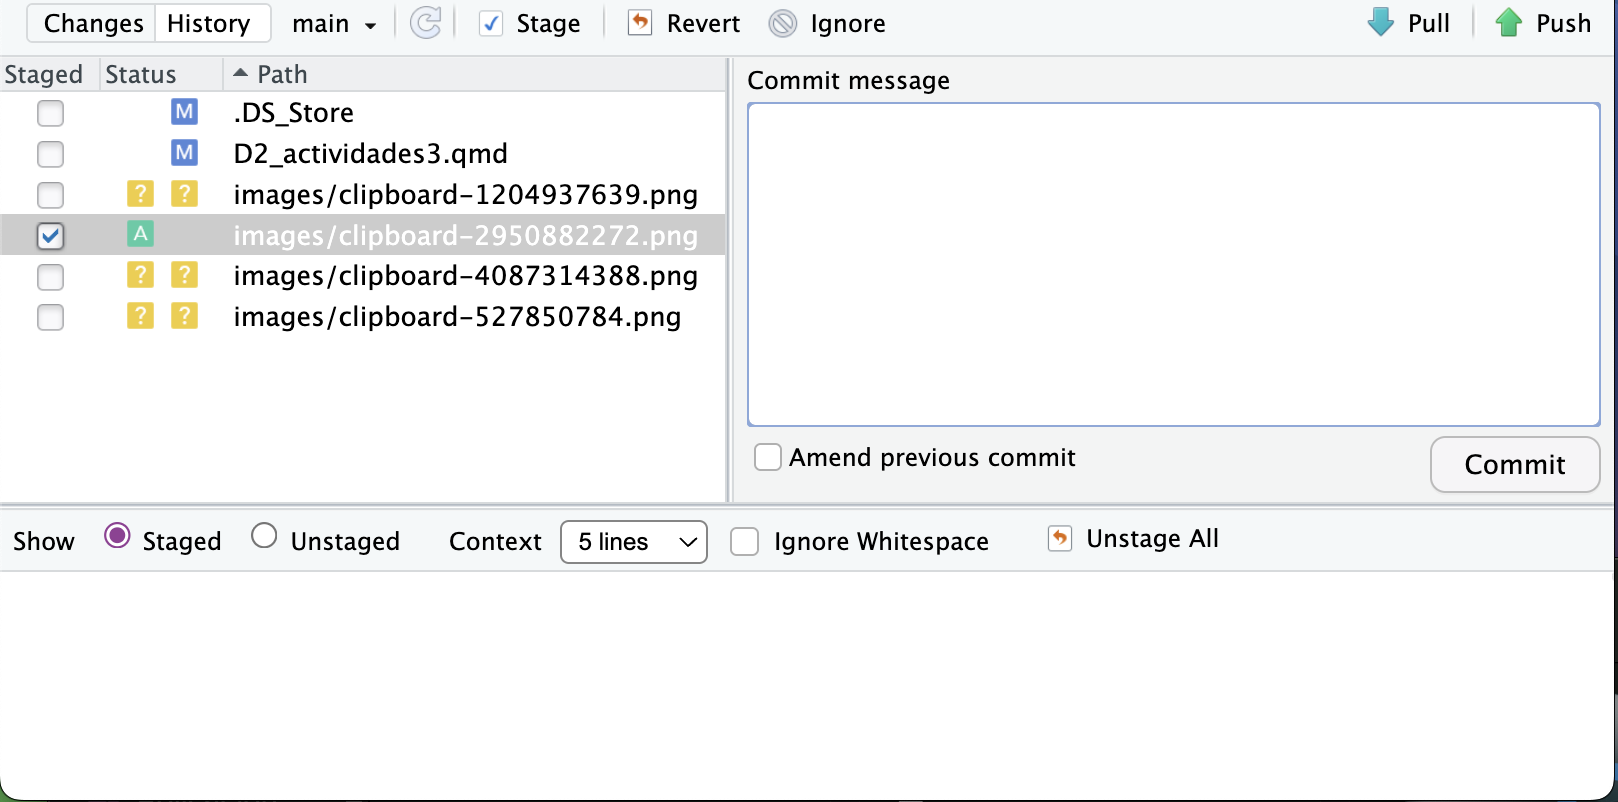
\includegraphics[keepaspectratio]{figures/clipboard-469430026.png}}

\begin{enumerate}
\def\labelenumi{\arabic{enumi}.}
\setcounter{enumi}{4}
\item
  \textbf{Sincronizar con GitHub}

  \begin{itemize}
  \item
    Usa los botones \emph{Push} (subir cambios al repositorio remoto) y
    \emph{Pull} (traer cambios del remoto).
  \item
    Normalmente, después de un commit local, harás \emph{Push} para que
    tus cambios aparezcan en GitHub.
  \end{itemize}
\end{enumerate}

\chapter{📙 Actividad 3D: Ediciones paso a paso en el
YAML}\label{actividad-3d-ediciones-paso-a-paso-en-el-yaml}

Instalar los paquetes:

\begin{Shaded}
\begin{Highlighting}[]
\FunctionTok{install.packages}\NormalTok{(}\StringTok{"postcards"}\NormalTok{)}
\FunctionTok{install.packages}\NormalTok{(}\StringTok{"fontawesome"}\NormalTok{)}
\end{Highlighting}
\end{Shaded}

Vamos a modificar paso a paso el YAML encontrado este archivo
\href{https://github.com/EveliaCoss/EveliaCoss.github.io/blob/main/index.Rmd}{index.Rmd}.

\begin{enumerate}
\def\labelenumi{\arabic{enumi}.}
\tightlist
\item
  Modifica tu nombre y agrega tu fotografía.
\end{enumerate}

\begin{verbatim}
---
title: "Evelia Coss" # <- Cambia por tu nombre
image: "yo_azul.jpg" # <- Coloca tu foto, recuerda checar la extensión del archivo
\end{verbatim}

Esta siguiente parte configura los botones que aparecen en tu página
web, los que ves aquí:

\pandocbounded{
\includegraphics[keepaspectratio]{figures/clipboard-2215590841.png}}

Los \textbf{botones} se componen de 3 cosas:

\begin{itemize}
\tightlist
\item
  \texttt{url}: la dirección web que apunta a la red social o página
  deseada.
\item
  \texttt{label}\textbf{(etiqueta)}: el texto visible del botón, que
  puede incluir tanto el nombre como el ícono.
\item
  ícono: un símbolo gráfico proveniente de
  \href{https://fontawesome.com/}{\textbf{Font Awesome}}, renderizado en
  R mediante el paquete \texttt{fontawesome}.
\end{itemize}

De esta forma, el botón combina funcionalidad (el enlace), legibilidad
(la etiqueta) y diseño visual (el ícono), ofreciendo una experiencia más
atractiva y clara para el usuario.

\begin{enumerate}
\def\labelenumi{\arabic{enumi}.}
\setcounter{enumi}{1}
\tightlist
\item
  Ahora, modifica el \texttt{url} agregando tu información:
\end{enumerate}

\begin{verbatim}
links:
  - label: '![](s5_actividades3_files/figure-pdf/fa-icon-040417c26d62b1cb437879a9ea999e9f.pdf){height=1em width=0.88em} LinkedIn'
    url: "https://www.linkedin.com/in/evelia-lorena-coss-navarrete-562226229/"
  - label: '![](s5_actividades3_files/figure-pdf/fa-icon-4477dfc8f6171a691064ec5228c14233.pdf){height=1em width=1em} Twitter'
    url: "https://twitter.com/EveliaCoss/"
  - label: '![](s5_actividades3_files/figure-pdf/fa-icon-76068811295de95578186b75aa40f62a.pdf){height=1em width=0.97em} Github'
    url: "https://github.com/EveliaCoss/"
  - label: '![](s5_actividades3_files/figure-pdf/fa-icon-00c32f2f2d7414e3e9add5c5fede8670.pdf){height=1em width=1em} Mail'
    url: "mailto:ecoss@liigh.unam.mx"
  - label: '![](s5_actividades3_files/figure-pdf/fa-icon-e5ec9ba13b56360902b281691d1f47ef.pdf){height=1em width=0.88em} CV'
    url: "https://eveliacoss.github.io/CV/cv_ECoss.html"
\end{verbatim}

\begin{tcolorbox}[enhanced jigsaw, arc=.35mm, bottomrule=.15mm, bottomtitle=1mm, breakable, colback=white, colbacktitle=quarto-callout-note-color!10!white, colframe=quarto-callout-note-color-frame, coltitle=black, left=2mm, leftrule=.75mm, opacityback=0, opacitybacktitle=0.6, rightrule=.15mm, title=\textcolor{quarto-callout-note-color}{\faInfo}\hspace{0.5em}{Nota}, titlerule=0mm, toprule=.15mm, toptitle=1mm]

Si quieres buscar otro ícono puedes buscarlo directamente en la página
web \href{https://fontawesome.com/}{Font Awesome}. Solo si aparece
podriamos agregarlo.

\end{tcolorbox}

\begin{enumerate}
\def\labelenumi{\arabic{enumi}.}
\setcounter{enumi}{2}
\tightlist
\item
  Modificar el \textbf{estilo} del postcards entrando al sitio web de
  \href{https://github.com/seankross/postcards}{postcards}.
\end{enumerate}

Cambia el nombre de \texttt{jolla} por otro.

\begin{verbatim}
output:
  postcards::jolla
---  
\end{verbatim}

\begin{tcolorbox}[enhanced jigsaw, arc=.35mm, bottomrule=.15mm, bottomtitle=1mm, breakable, colback=white, colbacktitle=quarto-callout-caution-color!10!white, colframe=quarto-callout-caution-color-frame, coltitle=black, left=2mm, leftrule=.75mm, opacityback=0, opacitybacktitle=0.6, rightrule=.15mm, title=\textcolor{quarto-callout-caution-color}{\faFire}\hspace{0.5em}{Precaución}, titlerule=0mm, toprule=.15mm, toptitle=1mm]

El estilo \texttt{onofre} tiene problemas para renderizarse bien.

\end{tcolorbox}

\begin{enumerate}
\def\labelenumi{\arabic{enumi}.}
\setcounter{enumi}{3}
\tightlist
\item
  Da clic en Knit o en la bolita de estambre.
\item
  Guarda los cambios en GitHub a través de Rstudio.
\item
  Visualiza tu pagina web en línea, en mi casi es desde:
  \url{https://eveliacoss.github.io/}
\end{enumerate}

\pandocbounded{\includegraphics[keepaspectratio]{figures/clipboard-969675420.png}}

Imagen tomada de:
\href{https://allisonhorst.com/horst-hill-collaborations}{Allison Horst}

\section{Referencias}\label{referencias-17}

\begin{itemize}
\tightlist
\item
  \href{https://allisonhorst.com/horst-hill-collaborations}{Allison
  Horst}
\item
  \url{https://github.com/EveliaCoss/EveliaCoss.github.io}
\item
  \href{https://github.com/seankross/postcards}{postcards}
\end{itemize}

\chapter{Introducción a Quarto}\label{introducciuxf3n-a-quarto-1}

\begin{quote}
\textbf{Fecha:} 13 de octubre, 2026
\end{quote}

\textbf{Quarto} es una versión multilingüe y
\href{https://quarto.org/docs/faq/rmarkdown.html}{de última generación}
de R Markdown de Posit que incluye docenas de nuevas características y
capacidades y al mismo tiempo puede renderizar la mayoría de los
archivos Rmd existentes sin modificaciones.

\begin{itemize}
\tightlist
\item
  Extensión \texttt{.qmd}
\item
  Sintaxis de Markdown para el texto
\item
  Tipos de archivos puede ser \hyperref[0]{HTML} , \hyperref[0]{PDF} ,
  documento \hyperref[0]{de MS Word , presentación} , \hyperref[0]{sitio
  web} , \hyperref[0]{libro} , \hyperref[0]{documento interactivo} u
  \hyperref[0]{otro formato} .
\end{itemize}

\begin{center}
\pandocbounded{\includegraphics[keepaspectratio]{images/clipboard-2661750054.png}}
\end{center}

\section{¿Cómo funciona?}\label{cuxf3mo-funciona-2}

Utiliza el botón
\includegraphics[width=0.20833in,height=0.17708in]{index_files/mediabag/rstudio-render-butto.png}
\textbf{Render} en el IDE de RStudio para renderizar el archivo y
obtener una vista previa de la salida con un solo clic o un atajo de
teclado (⇧⌘K).

\pandocbounded{\includegraphics[keepaspectratio]{images/clipboard-3479006155.png}}

Si prefiere renderizar automáticamente al guardar, puede activar la
opción ``Renderizar al guardar'' en la barra de herramientas del editor.
La vista previa se actualizará al volver a renderizar el documento. La
vista previa en paralelo funciona tanto con HTML como con PDF.

\pandocbounded{\includegraphics[keepaspectratio]{images/clipboard-2728400971.png}}

Al renderizar un documento de Quarto,
\href{http://yihui.name/knitr/}{knitr} ejecuta primero todos los
fragmentos de código y crea un nuevo documento Markdown (.md), que
incluye el código y su salida. El archivo Markdown generado es procesado
por \href{http://pandoc.org/}{pandoc} , que crea el formato final. El
botón Renderizar encapsula estas acciones y las ejecuta en el orden
correcto.

\pandocbounded{\includegraphics[keepaspectratio]{images/clipboard-318997387.png}}

\section{¿Cómo se compone?}\label{cuxf3mo-se-compone-1}

El archivo contiene tres tipos de contenido: \textbf{un encabezado YAML,
fragmentos de código} y \textbf{texto Markdown}.

\subsection{\texorpdfstring{\textbf{encabezado
YAML}}{encabezado YAML}}\label{encabezado-yaml-1}

Un encabezado YAML (opcional) delimitado por tres guiones (
\texttt{-\/-\/-}) en cada extremo.

\begin{verbatim}
---
title: "Hello, Quarto"
format: html
editor: visual
---
\end{verbatim}

Al renderizar, el símbolo \texttt{title}, \texttt{"Hello,\ Quarto"},
aparecerá en la parte superior del documento renderizado con un tamaño
de fuente mayor que el resto del documento. Los otros dos campos YAML
indican que la salida debe estar en formato \texttt{html}
\texttt{format}y que el documento debe abrirse en formato
\texttt{visual} \texttt{editor}predeterminado.

Puedes consultar todos los campos YAML disponibles para documentos: HTML
\href{https://quarto.org/docs/reference/formats/html.html}{aquí} . Los
campos YAML disponibles varían según el formato del documento; por
ejemplo, consulte
\href{https://quarto.org/docs/reference/formats/pdf.html}{aquí} los
campos YAML para documentos PDF y
\href{https://quarto.org/docs/reference/formats/docx.html}{aquí} para MS
Word.

\begin{tcolorbox}[enhanced jigsaw, arc=.35mm, bottomrule=.15mm, bottomtitle=1mm, breakable, colback=white, colbacktitle=quarto-callout-important-color!10!white, colframe=quarto-callout-important-color-frame, coltitle=black, left=2mm, leftrule=.75mm, opacityback=0, opacitybacktitle=0.6, rightrule=.15mm, title=\textcolor{quarto-callout-important-color}{\faExclamation}\hspace{0.5em}{Importante}, titlerule=0mm, toprule=.15mm, toptitle=1mm]

Para crear archivos PDF, se necesitará instalar una distribución
reciente de \href{https://www.latex-project.org/}{LaTeX}. Recomendamos
usar TinyTeX (basado en TexLive), que se puede instalar con el siguiente
comando:

\begin{Shaded}
\begin{Highlighting}[]
\ExtensionTok{quarto}\NormalTok{ install tinytex}
\end{Highlighting}
\end{Shaded}

\end{tcolorbox}

\section{Renderizar a varios tipos de
archivos}\label{renderizar-a-varios-tipos-de-archivos-1}

Si desea renderizar en todos los formatos, puede hacerlo con el paquete
\href{https://github.com/quarto-dev/quarto-r}{\textbf{quarto}} , que
proporciona una interfaz de R para la CLI de Quarto. Por ejemplo, para
renderizar el documento actual, utilice
\texttt{quarto::quarto\_render()}. También puede especificar el nombre
del documento que desea renderizar, así como los formatos de salida.

\begin{Shaded}
\begin{Highlighting}[]
\ExtensionTok{quarto::quarto\_render}\ErrorTok{(}
  \StringTok{"authoring.qmd"}\ExtensionTok{,} 
  \ExtensionTok{output\_format}\NormalTok{ = c}\ErrorTok{(}\StringTok{"pdf"}\ExtensionTok{,} \StringTok{"html"}\NormalTok{, }\StringTok{"docx"}\KeywordTok{)}
\KeywordTok{)}
\end{Highlighting}
\end{Shaded}

Como resultado, verá aparecer tres nuevos archivos en el panel Archivos:

\begin{itemize}
\tightlist
\item
  \texttt{authoring.docx}
\item
  \texttt{authoring.html}
\item
  \texttt{authoring.pdf}
\end{itemize}

\pandocbounded{\includegraphics[keepaspectratio]{images/clipboard-365079727.png}}

\section{Callout / notas}\label{callout-notas-1}

Da clic en Insert/callout.

Puede seleccionar uno de los cinco tipos de callout (nota, sugerencia,
importante, precaución o advertencia), personalizar su apariencia
(predeterminada, simple o mínima) y decidir si desea mostrar el ícono.

\pandocbounded{\includegraphics[keepaspectratio]{images/clipboard-3099889024.png}}

Luego, intente insertar el texto dentro del cuadro de callout.

\begin{tcolorbox}[enhanced jigsaw, arc=.35mm, bottomrule=.15mm, bottomtitle=1mm, breakable, colback=white, colbacktitle=quarto-callout-note-color!10!white, colframe=quarto-callout-note-color-frame, coltitle=black, left=2mm, leftrule=.75mm, opacityback=0, opacitybacktitle=0.6, rightrule=.15mm, title=\textcolor{quarto-callout-note-color}{\faInfo}\hspace{0.5em}{Nota}, titlerule=0mm, toprule=.15mm, toptitle=1mm]

Nota

\end{tcolorbox}

\begin{tcolorbox}[enhanced jigsaw, arc=.35mm, bottomrule=.15mm, bottomtitle=1mm, breakable, colback=white, colbacktitle=quarto-callout-tip-color!10!white, colframe=quarto-callout-tip-color-frame, coltitle=black, left=2mm, leftrule=.75mm, opacityback=0, opacitybacktitle=0.6, rightrule=.15mm, title=\textcolor{quarto-callout-tip-color}{\faLightbulb}\hspace{0.5em}{Tip}, titlerule=0mm, toprule=.15mm, toptitle=1mm]

Sugerencia

\end{tcolorbox}

\begin{tcolorbox}[enhanced jigsaw, arc=.35mm, bottomrule=.15mm, bottomtitle=1mm, breakable, colback=white, colbacktitle=quarto-callout-important-color!10!white, colframe=quarto-callout-important-color-frame, coltitle=black, left=2mm, leftrule=.75mm, opacityback=0, opacitybacktitle=0.6, rightrule=.15mm, title=\textcolor{quarto-callout-important-color}{\faExclamation}\hspace{0.5em}{Importante}, titlerule=0mm, toprule=.15mm, toptitle=1mm]

Importante

\end{tcolorbox}

\begin{tcolorbox}[enhanced jigsaw, arc=.35mm, bottomrule=.15mm, bottomtitle=1mm, breakable, colback=white, colbacktitle=quarto-callout-caution-color!10!white, colframe=quarto-callout-caution-color-frame, coltitle=black, left=2mm, leftrule=.75mm, opacityback=0, opacitybacktitle=0.6, rightrule=.15mm, title=\textcolor{quarto-callout-caution-color}{\faFire}\hspace{0.5em}{Precaución}, titlerule=0mm, toprule=.15mm, toptitle=1mm]

Precaución

\end{tcolorbox}

\begin{tcolorbox}[enhanced jigsaw, arc=.35mm, bottomrule=.15mm, bottomtitle=1mm, breakable, colback=white, colbacktitle=quarto-callout-warning-color!10!white, colframe=quarto-callout-warning-color-frame, coltitle=black, left=2mm, leftrule=.75mm, opacityback=0, opacitybacktitle=0.6, rightrule=.15mm, title=\textcolor{quarto-callout-warning-color}{\faExclamationTriangle}\hspace{0.5em}{Advertencia}, titlerule=0mm, toprule=.15mm, toptitle=1mm]

Advertencia

\end{tcolorbox}

\section{Cross reference / Referencias
cruzadas}\label{cross-reference-referencias-cruzadas-1}

Las \textbf{cross references} en Quarto son una forma de enlazar
automáticamente figuras, tablas, secciones, ecuaciones y otros elementos
dentro de tu documento, de manera que se numeran y se convierten en
hipervínculos navegables. Esto evita tener que actualizar manualmente la
numeración si agregas o quitas elementos.

\begin{enumerate}
\def\labelenumi{\arabic{enumi}.}
\item
  \textbf{Etiqueta (label)} Cada elemento que quieras referenciar
  necesita una etiqueta única.

  \begin{itemize}
  \tightlist
  \item
    Para figuras: \texttt{\{\#fig-nombre\}}
  \item
    Para tablas: \texttt{\{\#tbl-nombre\}}
  \item
    Para secciones: \texttt{\{\#sec-nombre\}}
  \item
    Para ecuaciones: \texttt{\{\#eq-nombre\}}
  \end{itemize}
\item
  \textbf{Referencia en el texto} Para referenciar, se usa \texttt{@}
  seguido del identificador:

  \begin{itemize}
  \tightlist
  \item
    \texttt{@fig-nombre} → referencia a una figura.
  \item
    \texttt{@tbl-nombre} → referencia a una tabla.
  \item
    \texttt{@sec-nombre} → referencia a una sección.
  \item
    \texttt{@eq-nombre} → referencia a una ecuación.
  \end{itemize}
\end{enumerate}

Quarto asigna números consecutivos a las entidades (Figura 1, Tabla 2,
etc.) y actualiza todo si cambias el orden o agregas nuevos elementos.

Ejemplo:

{\def\LTcaptype{none} % do not increment counter
\begin{longtable}[]{@{}
  >{\raggedright\arraybackslash}p{(\linewidth - 4\tabcolsep) * \real{0.1091}}
  >{\raggedright\arraybackslash}p{(\linewidth - 4\tabcolsep) * \real{0.1636}}
  >{\raggedright\arraybackslash}p{(\linewidth - 4\tabcolsep) * \real{0.7182}}@{}}
\toprule\noalign{}
\begin{minipage}[b]{\linewidth}\raggedright
Entidad
\end{minipage} & \begin{minipage}[b]{\linewidth}\raggedright
Referencia
\end{minipage} & \begin{minipage}[b]{\linewidth}\raggedright
Etiqueta / Título
\end{minipage} \\
\midrule\noalign{}
\endhead
\bottomrule\noalign{}
\endlastfoot
Sección & \texttt{@sec-eda} &
\begin{minipage}[t]{\linewidth}\raggedright
ID añadido al encabezado:

\begin{verbatim}
# Análisis exploratorio de datos {#sec-eda}
\end{verbatim}
\end{minipage} \\
Figura & \texttt{@fig-pressure} &
\begin{minipage}[t]{\linewidth}\raggedright
Opciones YAML en la celda de código:

\begin{verbatim}
#| label: fig-scatterplot
#| fig-cap: "Pressure"
\end{verbatim}
\end{minipage} \\
Tabla & \texttt{@tbl-stats} &
\begin{minipage}[t]{\linewidth}\raggedright
Opciones YAML en la celda de código:

\begin{verbatim}
#| label: tbl-stats
#| tbl-cap: "Summary statistics for price and area of houses in Duke Forest"
\end{verbatim}
\end{minipage} \\
Ecuación & \texttt{@eq-slr} &
\begin{minipage}[t]{\linewidth}\raggedright
Al final de la ecuación de visualización:

\begin{verbatim}
$$ {#eq-slr}
\end{verbatim}
\end{minipage} \\
\end{longtable}
}

\chapter{Análisis exploratorio de datos}\label{sec-eda}

Aquí se describe el análisis exploratorio de los datos.

\begin{Shaded}
\begin{Highlighting}[]
\FunctionTok{library}\NormalTok{(ggplot2)}
\NormalTok{dat }\OtherTok{\textless{}{-}} \FunctionTok{data.frame}\NormalTok{(}\AttributeTok{cond =} \FunctionTok{rep}\NormalTok{(}\FunctionTok{c}\NormalTok{(}\StringTok{"A"}\NormalTok{, }\StringTok{"B"}\NormalTok{), }\AttributeTok{each=}\DecValTok{10}\NormalTok{),}
                  \AttributeTok{xvar =} \DecValTok{1}\SpecialCharTok{:}\DecValTok{20} \SpecialCharTok{+} \FunctionTok{rnorm}\NormalTok{(}\DecValTok{20}\NormalTok{,}\AttributeTok{sd=}\DecValTok{3}\NormalTok{),}
                  \AttributeTok{yvar =} \DecValTok{1}\SpecialCharTok{:}\DecValTok{20} \SpecialCharTok{+} \FunctionTok{rnorm}\NormalTok{(}\DecValTok{20}\NormalTok{,}\AttributeTok{sd=}\DecValTok{3}\NormalTok{))}

\FunctionTok{ggplot}\NormalTok{(dat, }\FunctionTok{aes}\NormalTok{(}\AttributeTok{x=}\NormalTok{xvar, }\AttributeTok{y=}\NormalTok{yvar)) }\SpecialCharTok{+}
    \FunctionTok{geom\_point}\NormalTok{(}\AttributeTok{shape=}\DecValTok{1}\NormalTok{) }\SpecialCharTok{+} 
    \FunctionTok{geom\_smooth}\NormalTok{() }
\end{Highlighting}
\end{Shaded}

\begin{verbatim}
`geom_smooth()` using method = 'loess' and formula = 'y ~ x'
\end{verbatim}

\begin{figure}[H]

\centering{

\pandocbounded{
\includegraphics[keepaspectratio]{Intro_Quarto_files/figure-pdf/fig-pressure-1.pdf}}

}

\caption{\label{fig-pressure}Pressure}

\end{figure}%

\section{Estadísticas descriptivas}\label{sec-stats}

\begin{Shaded}
\begin{Highlighting}[]
\NormalTok{knitr}\SpecialCharTok{::}\FunctionTok{kable}\NormalTok{(}\FunctionTok{head}\NormalTok{(ggplot2}\SpecialCharTok{::}\NormalTok{diamonds))}
\end{Highlighting}
\end{Shaded}

{

\begin{longtable}[]{@{}
  >{\raggedleft\arraybackslash}p{(\linewidth - 18\tabcolsep) * \real{0.0952}}
  >{\raggedright\arraybackslash}p{(\linewidth - 18\tabcolsep) * \real{0.1587}}
  >{\raggedright\arraybackslash}p{(\linewidth - 18\tabcolsep) * \real{0.0952}}
  >{\raggedright\arraybackslash}p{(\linewidth - 18\tabcolsep) * \real{0.1270}}
  >{\raggedleft\arraybackslash}p{(\linewidth - 18\tabcolsep) * \real{0.0952}}
  >{\raggedleft\arraybackslash}p{(\linewidth - 18\tabcolsep) * \real{0.0952}}
  >{\raggedleft\arraybackslash}p{(\linewidth - 18\tabcolsep) * \real{0.0952}}
  >{\raggedleft\arraybackslash}p{(\linewidth - 18\tabcolsep) * \real{0.0794}}
  >{\raggedleft\arraybackslash}p{(\linewidth - 18\tabcolsep) * \real{0.0794}}
  >{\raggedleft\arraybackslash}p{(\linewidth - 18\tabcolsep) * \real{0.0794}}@{}}

\caption{\label{tbl-stats}Summary statistics for price and area of
houses in Duke Forest}

\tabularnewline

\toprule\noalign{}
\begin{minipage}[b]{\linewidth}\raggedleft
carat
\end{minipage} & \begin{minipage}[b]{\linewidth}\raggedright
cut
\end{minipage} & \begin{minipage}[b]{\linewidth}\raggedright
color
\end{minipage} & \begin{minipage}[b]{\linewidth}\raggedright
clarity
\end{minipage} & \begin{minipage}[b]{\linewidth}\raggedleft
depth
\end{minipage} & \begin{minipage}[b]{\linewidth}\raggedleft
table
\end{minipage} & \begin{minipage}[b]{\linewidth}\raggedleft
price
\end{minipage} & \begin{minipage}[b]{\linewidth}\raggedleft
x
\end{minipage} & \begin{minipage}[b]{\linewidth}\raggedleft
y
\end{minipage} & \begin{minipage}[b]{\linewidth}\raggedleft
z
\end{minipage} \\
\midrule\noalign{}
\endhead
\bottomrule\noalign{}
\endlastfoot
0.23 & Ideal & E & SI2 & 61.5 & 55 & 326 & 3.95 & 3.98 & 2.43 \\
0.21 & Premium & E & SI1 & 59.8 & 61 & 326 & 3.89 & 3.84 & 2.31 \\
0.23 & Good & E & VS1 & 56.9 & 65 & 327 & 4.05 & 4.07 & 2.31 \\
0.29 & Premium & I & VS2 & 62.4 & 58 & 334 & 4.20 & 4.23 & 2.63 \\
0.31 & Good & J & SI2 & 63.3 & 58 & 335 & 4.34 & 4.35 & 2.75 \\
0.24 & Very Good & J & VVS2 & 62.8 & 57 & 336 & 3.94 & 3.96 & 2.48 \\

\end{longtable}

}

\subsection{Modelo de regresión}\label{modelo-de-regresiuxf3n-1}

El modelo lineal simple se expresa como:

\[Y = \beta_0 + \beta_1 X + \epsilon\] \{\#eq-slr\}

Ejemplo en el texto:

Presentamos los resultados del análisis exploratorio de datos en
Capítulo~\ref{sec-eda} y la estadística descriptiva en
Sección~\ref{sec-stats} .

La Figura~\ref{fig-pressure} muestra la relación entre estas dos
variables en un diagrama de dispersión.

La Tabla~\ref{tbl-stats} presenta estadísticas descriptivas básicas de
estas dos variables.

Podemos ajustar un modelo de regresión lineal simple de la forma
mostrada en \textbf{?@eq-slr}.

\section{\texorpdfstring{\textbf{Aprendiendo
más}}{Aprendiendo más}}\label{aprendiendo-muxe1s-1}

¡Ya has aprendido los conceptos básicos de Quarto! Una vez que te
sientas cómodo creando y personalizando documentos, aquí tienes algunas
cosas más que puedes explorar:

\begin{itemize}
\item
  \href{https://quarto.org/docs/presentations/}{Presentaciones} : cree
  presentaciones de PowerPoint, Beamer y Revealjs utilizando la misma
  sintaxis que aprendió para crear documentos.
\item
  \href{https://quarto.org/docs/websites/}{Sitios web} : publique
  colecciones de documentos como un sitio web. Los sitios web admiten
  múltiples formas de navegación y búsqueda de texto completo.
\item
  \href{https://quarto.org/docs/websites/website-blog.html}{Blogs} :
  crea un blog con una página acerca de, listas de publicaciones
  flexibles, categorías, feeds RSS y más de veinte temas.
\item
  \href{https://quarto.org/docs/books/}{Libros} : cree libros y
  manuscritos en formatos impresos (PDF, MS Word) y en línea (HTML,
  ePub).
\item
  \href{https://quarto.org/docs/interactive/}{Interactividad} : incluya
  componentes interactivos para ayudar a los lectores a explorar los
  conceptos y los datos que está presentando más profundamente.
\end{itemize}

\pandocbounded{\includegraphics[keepaspectratio]{images/clipboard-1192798489.png}}

Imagen tomada de:
\href{https://allisonhorst.com/horst-hill-collaborations}{Allison Horst}

\section{Referencias}\label{referencias-18}

\begin{itemize}
\tightlist
\item
  \href{https://quarto.org/docs/get-started/hello/rstudio.html}{Tutorial:
  Hello, Quarto}
\end{itemize}

\chapter{\texorpdfstring{\textbf{📚} Actividad 4 y
5}{📚 Actividad 4 y 5}}\label{actividad-4-y-5}

\textbf{Fecha:} 19 de febrero, 2026

\section{\texorpdfstring{\textbf{📚} Actividad 4: Crear un documento de
Quarto con formato de salida
html}{📚 Actividad 4: Crear un documento de Quarto con formato de salida html}}\label{actividad-4-crear-un-documento-de-quarto-con-formato-de-salida-html}

Para crear un documento nuevo, ve a \textbf{Archivos/File}
\textgreater{} \textbf{Nuevo archivo} \textgreater{} \textbf{Documento
de Quarto.}

\pandocbounded{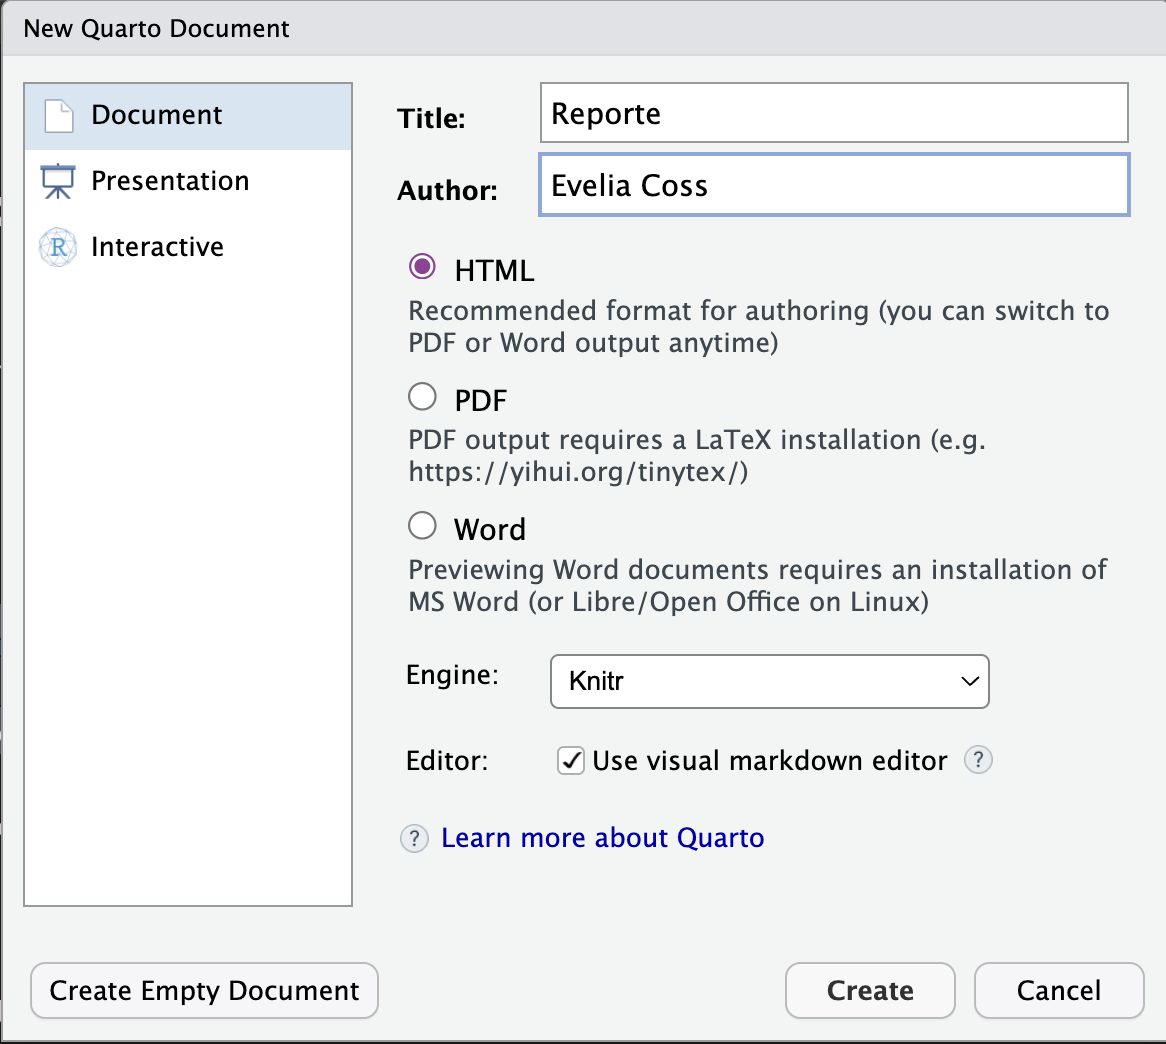
\includegraphics[keepaspectratio]{figures/Quarto_step1_new.png}}

Para este tipo de archivos vamos a usar la información del
\href{https://quarto.org/docs/reference/formats/html.html}{YAML para
HTML}.

\section{\texorpdfstring{\textbf{📚} Actividad 5: Explorar la galleria
de Quarto y elegir un
diseño}{📚 Actividad 5: Explorar la galleria de Quarto y elegir un diseño}}\label{actividad-5-explorar-la-galleria-de-quarto-y-elegir-un-diseuxf1o}

\begin{enumerate}
\def\labelenumi{\arabic{enumi}.}
\tightlist
\item
  Visita la \href{https://quarto.org/docs/gallery/}{galeria de Quarto}.
\item
  Ve al apartado de
  \href{https://quarto.org/docs/gallery/\#articles-reports}{Articles \&
  Reports}\textbf{.}
\end{enumerate}

\href{https://quarto.org/docs/gallery/}{\pandocbounded{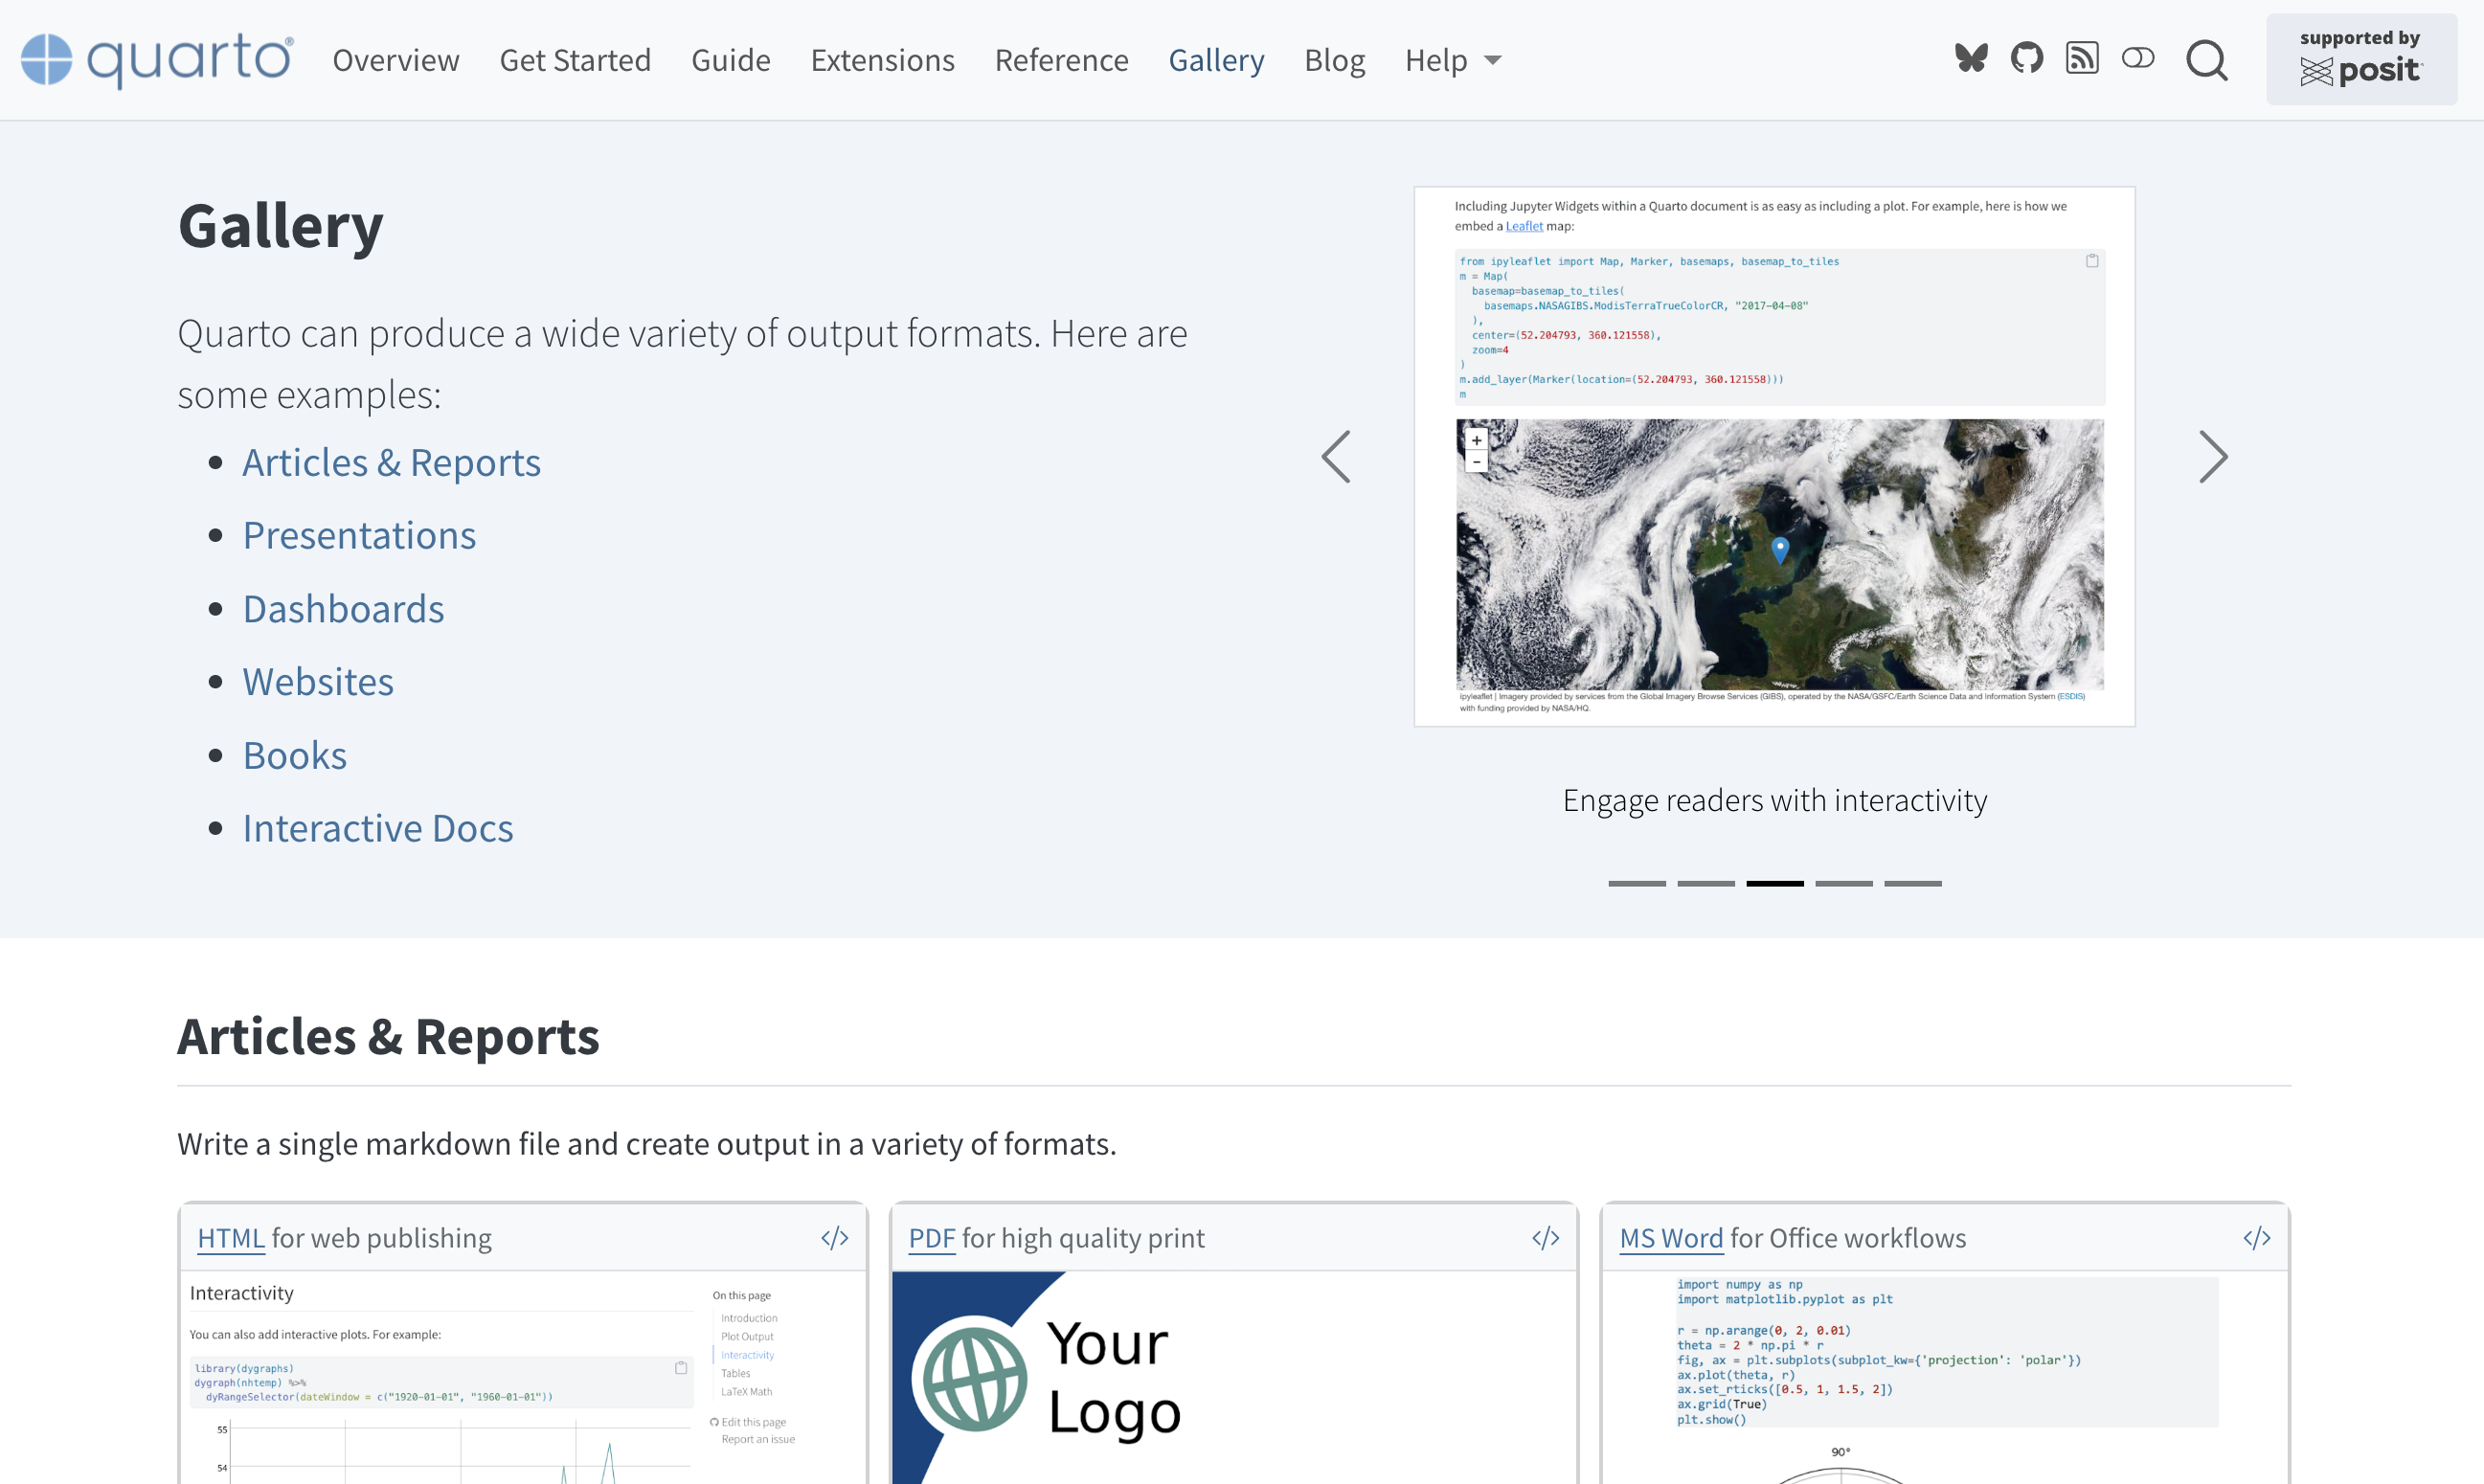
\includegraphics[keepaspectratio]{figures/Quarto_gallery.png}}}

\begin{enumerate}
\def\labelenumi{\arabic{enumi}.}
\setcounter{enumi}{2}
\tightlist
\item
  Selecciona un diseño y da clic en el botón
  ``\textless/\textgreater{}''.
\end{enumerate}

\pandocbounded{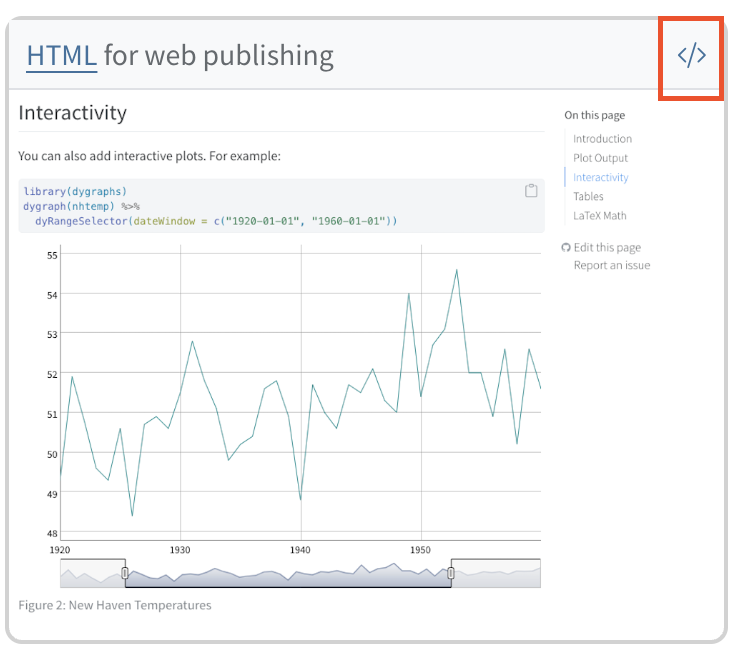
\includegraphics[keepaspectratio]{figures/Quarto_code.png}}

\begin{enumerate}
\def\labelenumi{\arabic{enumi}.}
\setcounter{enumi}{3}
\tightlist
\item
  Descarga el archivo desde GitHub y abrelo en Rstudio.
\end{enumerate}

\href{https://github.com/quarto-dev/quarto-gallery/blob/main/articles/html/html.qmd}{\pandocbounded{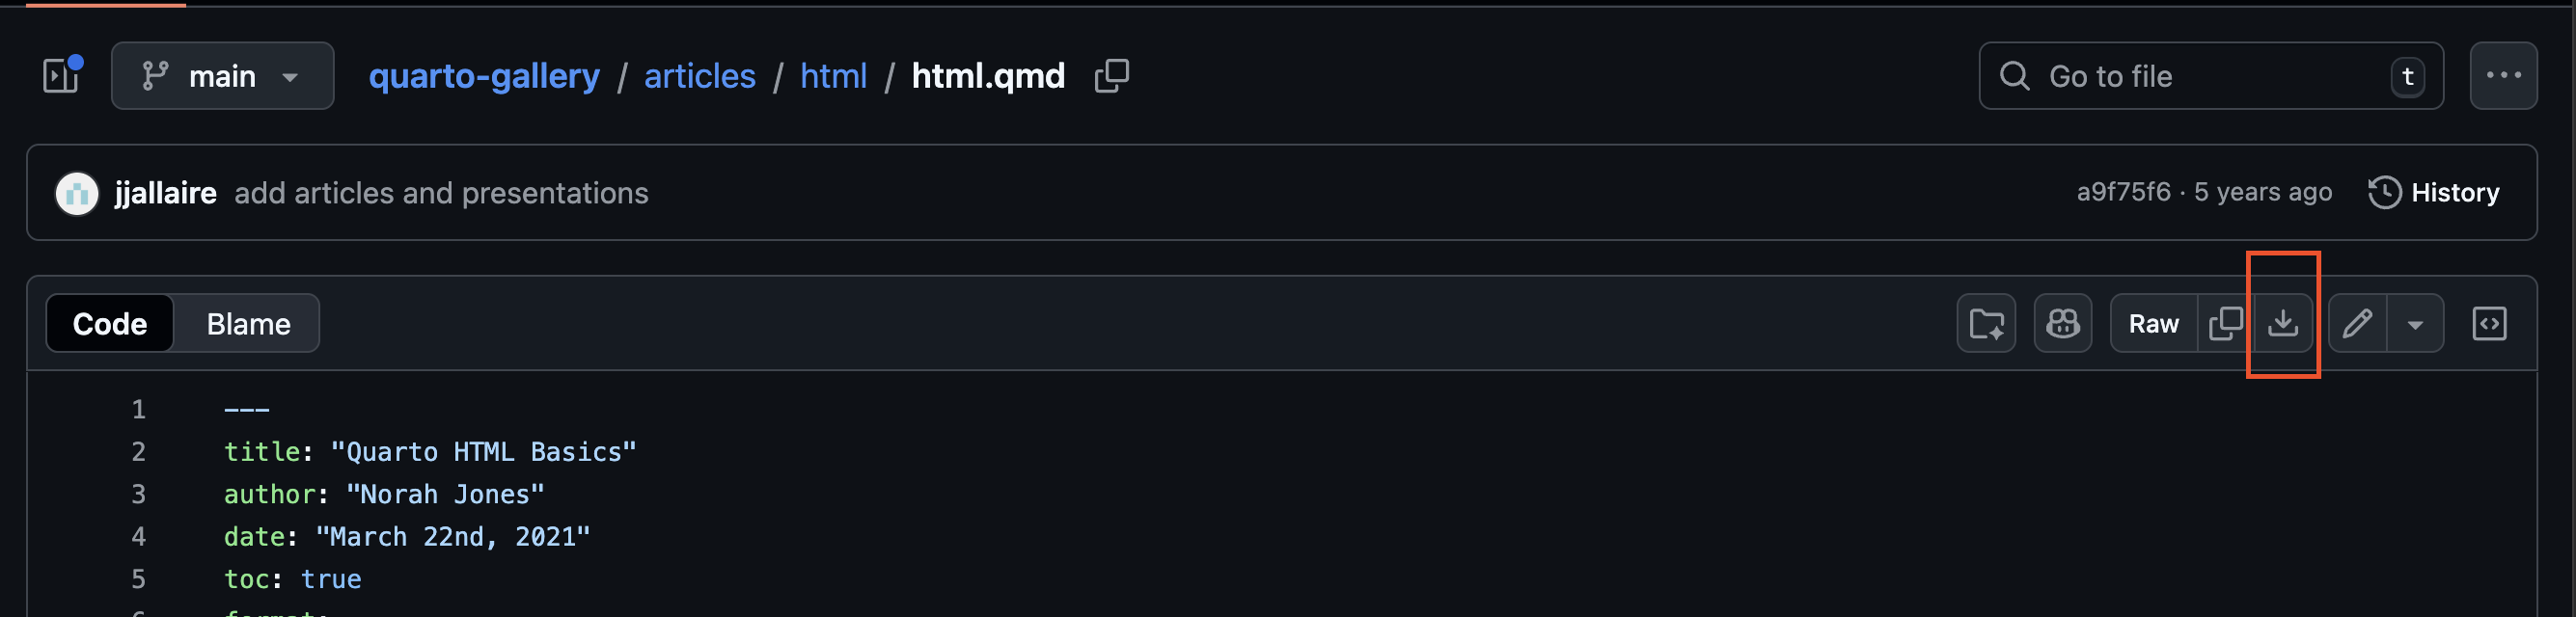
\includegraphics[keepaspectratio]{figures/GitHub_descargar.png}}}

\begin{tcolorbox}[enhanced jigsaw, arc=.35mm, bottomrule=.15mm, bottomtitle=1mm, breakable, colback=white, colbacktitle=quarto-callout-note-color!10!white, colframe=quarto-callout-note-color-frame, coltitle=black, left=2mm, leftrule=.75mm, opacityback=0, opacitybacktitle=0.6, rightrule=.15mm, title=\textcolor{quarto-callout-note-color}{\faInfo}\hspace{0.5em}{Nota}, titlerule=0mm, toprule=.15mm, toptitle=1mm]

Aquí les dejo mi ejemplo editado, ya que el ejemplo que descargaremos
tendrá algunos errores en su sintaxis.

\end{tcolorbox}

\section{Referencias}\label{referencias-19}

\begin{itemize}
\tightlist
\item
  \href{https://quarto.org/docs/get-started/hello/rstudio.html}{Tutorial:
  Hello, Quarto}
\end{itemize}

\part{\textbf{Sección 7} - Introducción a Python}

\chapter{\texorpdfstring{\textbf{📚} Actividad 4 y
5}{📚 Actividad 4 y 5}}\label{actividad-4-y-5-1}

\textbf{Fecha:} 19 de febrero, 2026

\section{\texorpdfstring{\textbf{📚} Actividad 4: Crear un documento de
Quarto con formato de salida
html}{📚 Actividad 4: Crear un documento de Quarto con formato de salida html}}\label{actividad-4-crear-un-documento-de-quarto-con-formato-de-salida-html-1}

Para crear un documento nuevo, ve a \textbf{Archivos/File}
\textgreater{} \textbf{Nuevo archivo} \textgreater{} \textbf{Documento
de Quarto.}

\pandocbounded{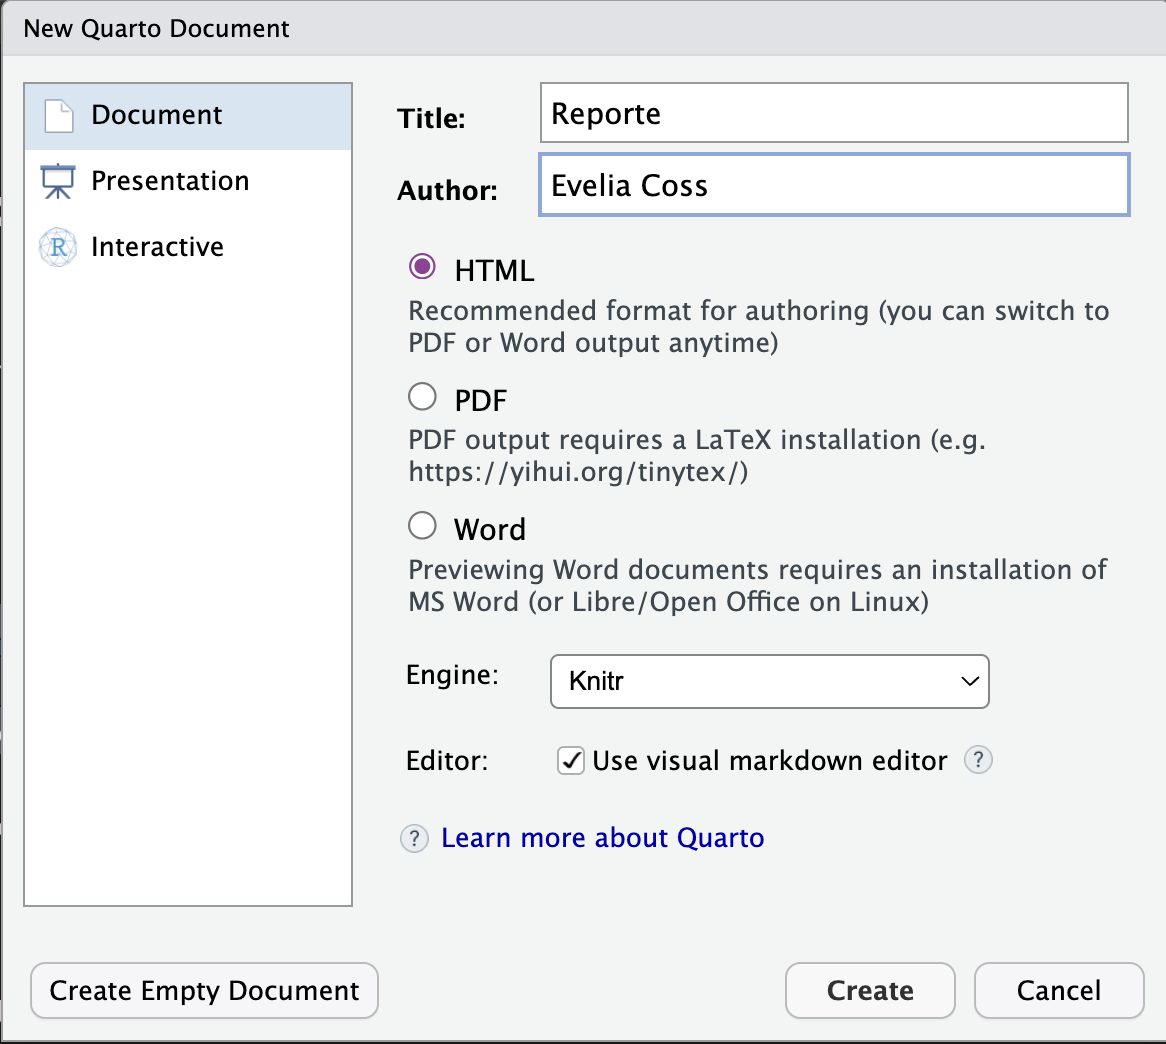
\includegraphics[keepaspectratio]{figures/Quarto_step1_new.png}}

Para este tipo de archivos vamos a usar la información del
\href{https://quarto.org/docs/reference/formats/html.html}{YAML para
HTML}.

\section{\texorpdfstring{\textbf{📚} Actividad 5: Explorar la galleria
de Quarto y elegir un
diseño}{📚 Actividad 5: Explorar la galleria de Quarto y elegir un diseño}}\label{actividad-5-explorar-la-galleria-de-quarto-y-elegir-un-diseuxf1o-1}

\begin{enumerate}
\def\labelenumi{\arabic{enumi}.}
\tightlist
\item
  Visita la \href{https://quarto.org/docs/gallery/}{galeria de Quarto}.
\item
  Ve al apartado de
  \href{https://quarto.org/docs/gallery/\#articles-reports}{Articles \&
  Reports}\textbf{.}
\end{enumerate}

\href{https://quarto.org/docs/gallery/}{\pandocbounded{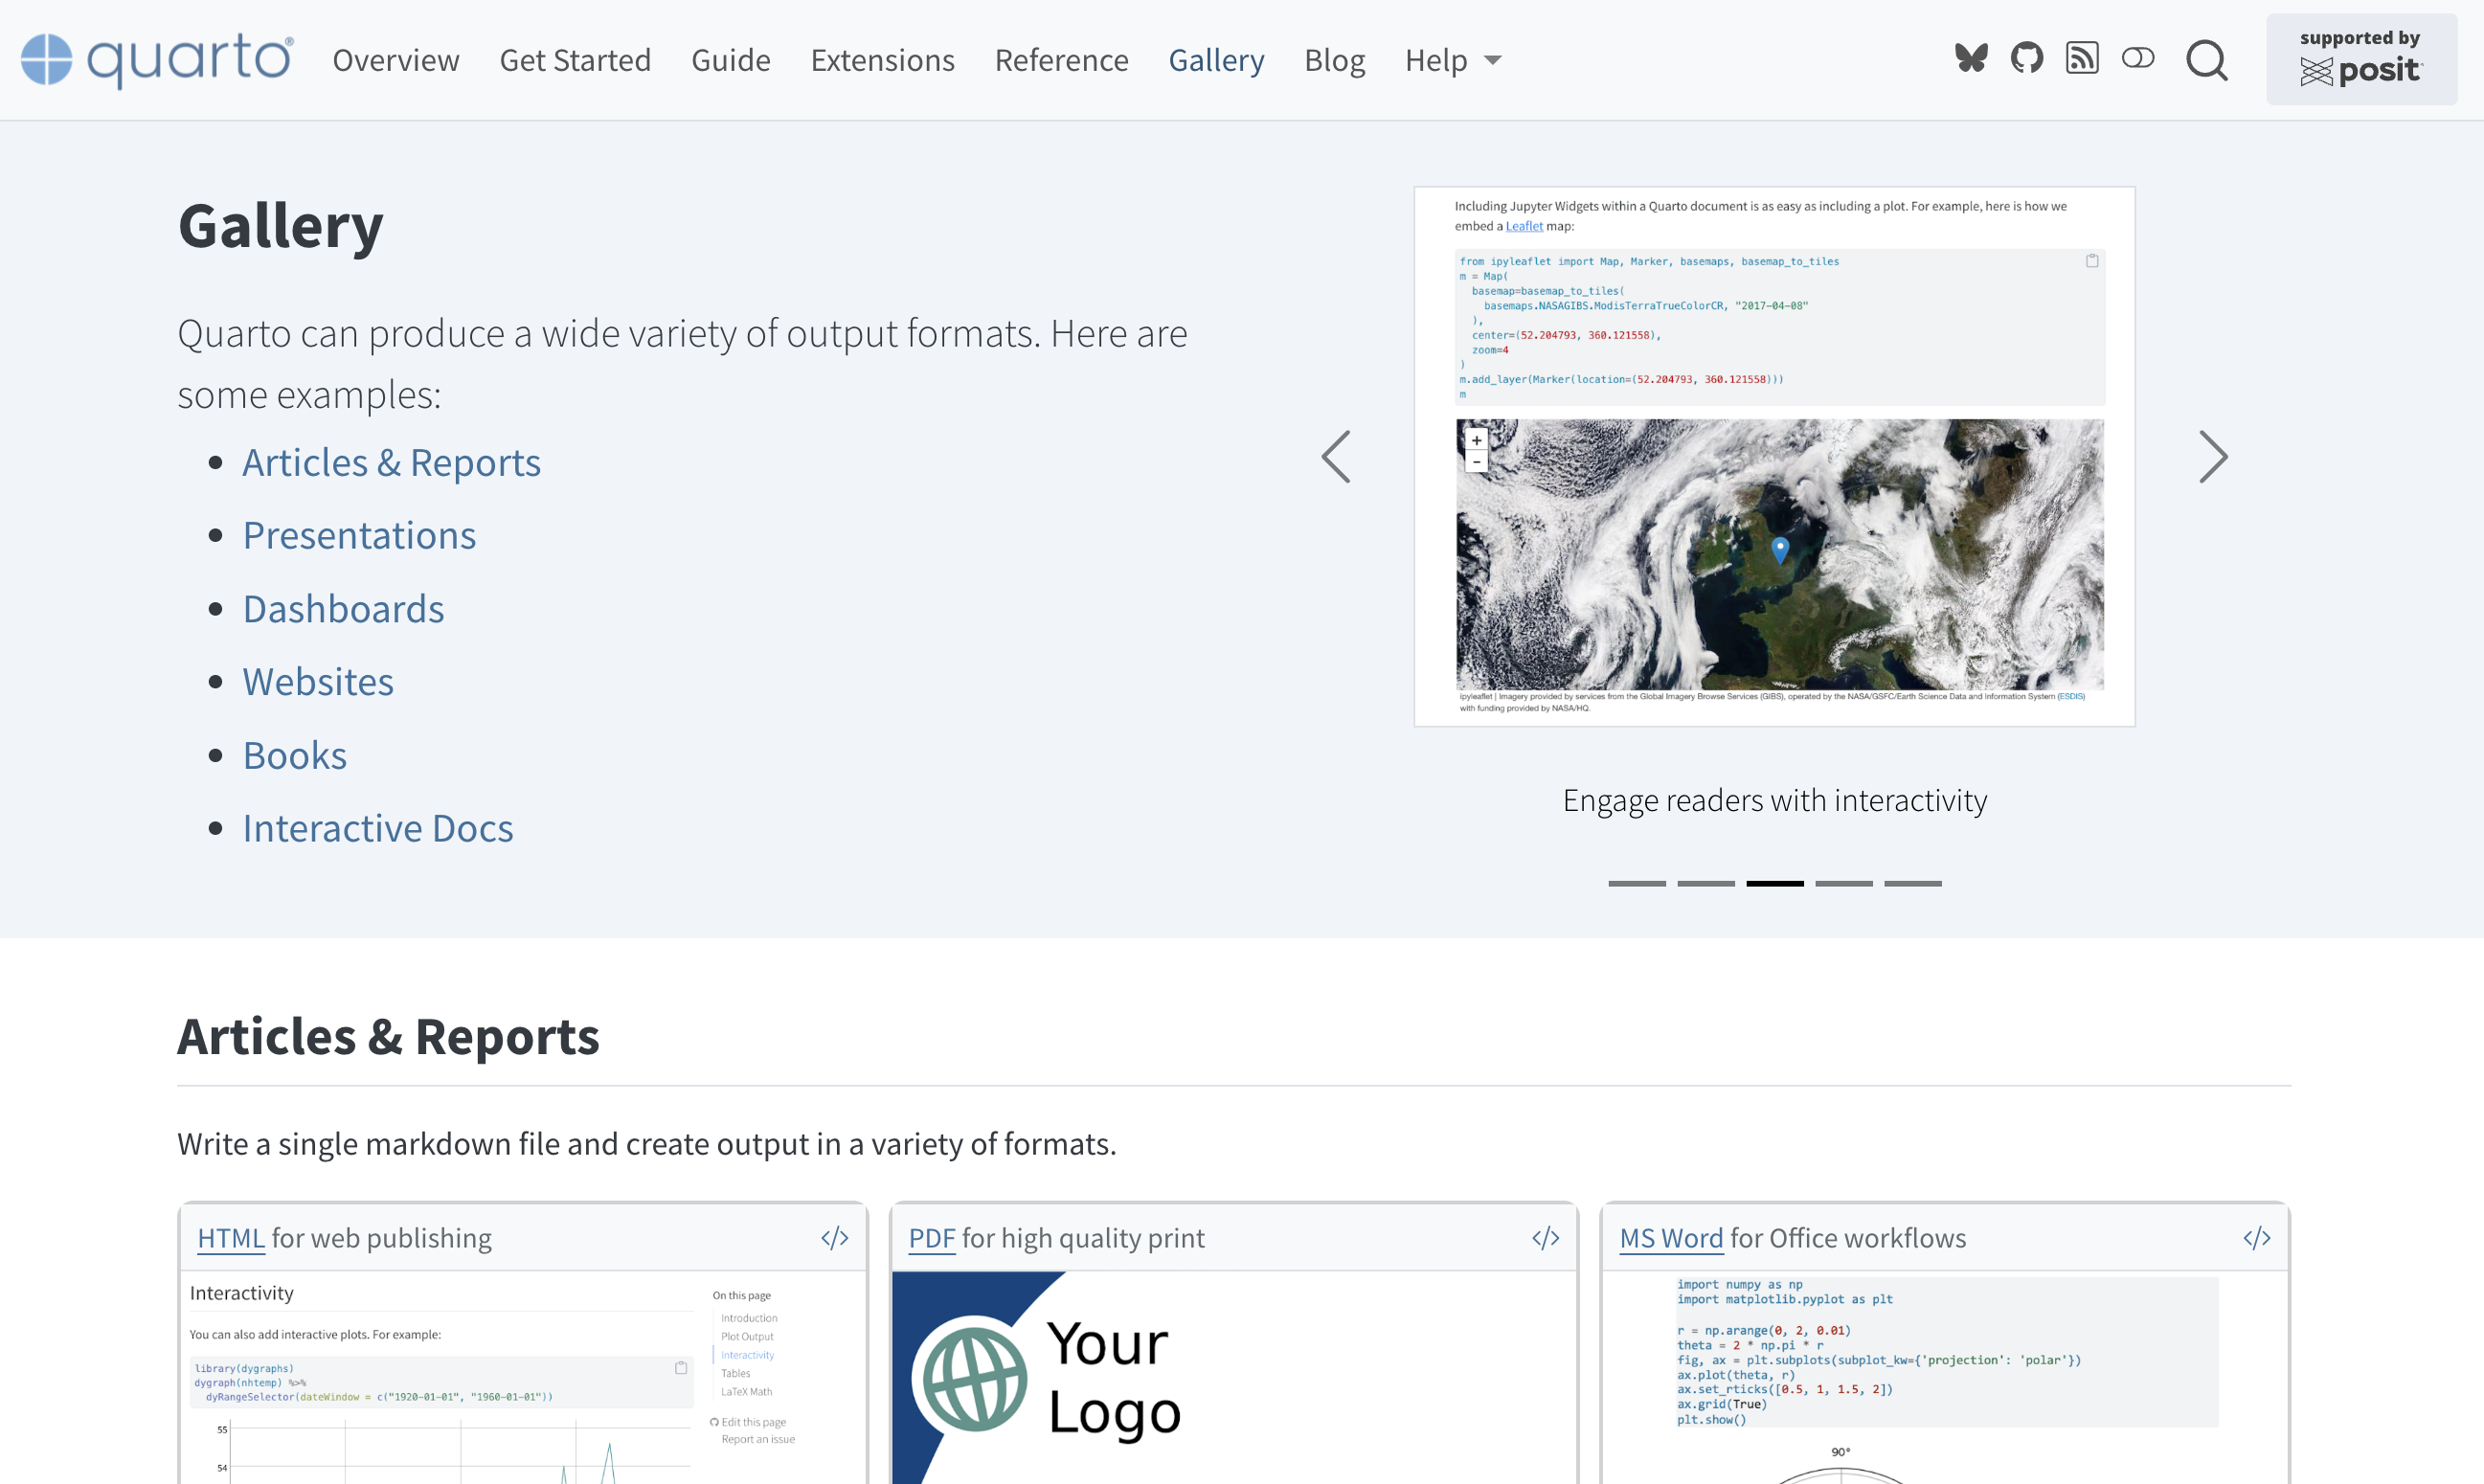
\includegraphics[keepaspectratio]{figures/Quarto_gallery.png}}}

\begin{enumerate}
\def\labelenumi{\arabic{enumi}.}
\setcounter{enumi}{2}
\tightlist
\item
  Selecciona un diseño y da clic en el botón
  ``\textless/\textgreater{}''.
\end{enumerate}

\pandocbounded{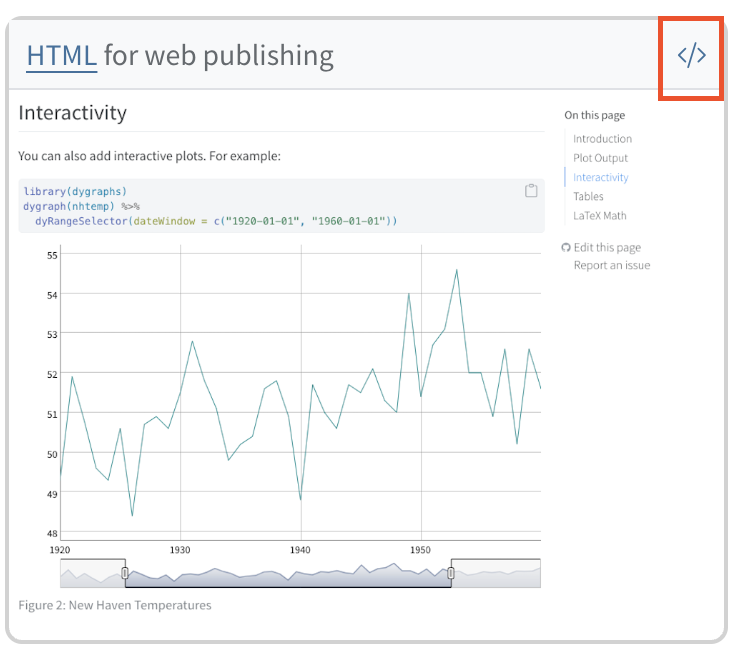
\includegraphics[keepaspectratio]{figures/Quarto_code.png}}

\begin{enumerate}
\def\labelenumi{\arabic{enumi}.}
\setcounter{enumi}{3}
\tightlist
\item
  Descarga el archivo desde GitHub y abrelo en Rstudio.
\end{enumerate}

\href{https://github.com/quarto-dev/quarto-gallery/blob/main/articles/html/html.qmd}{\pandocbounded{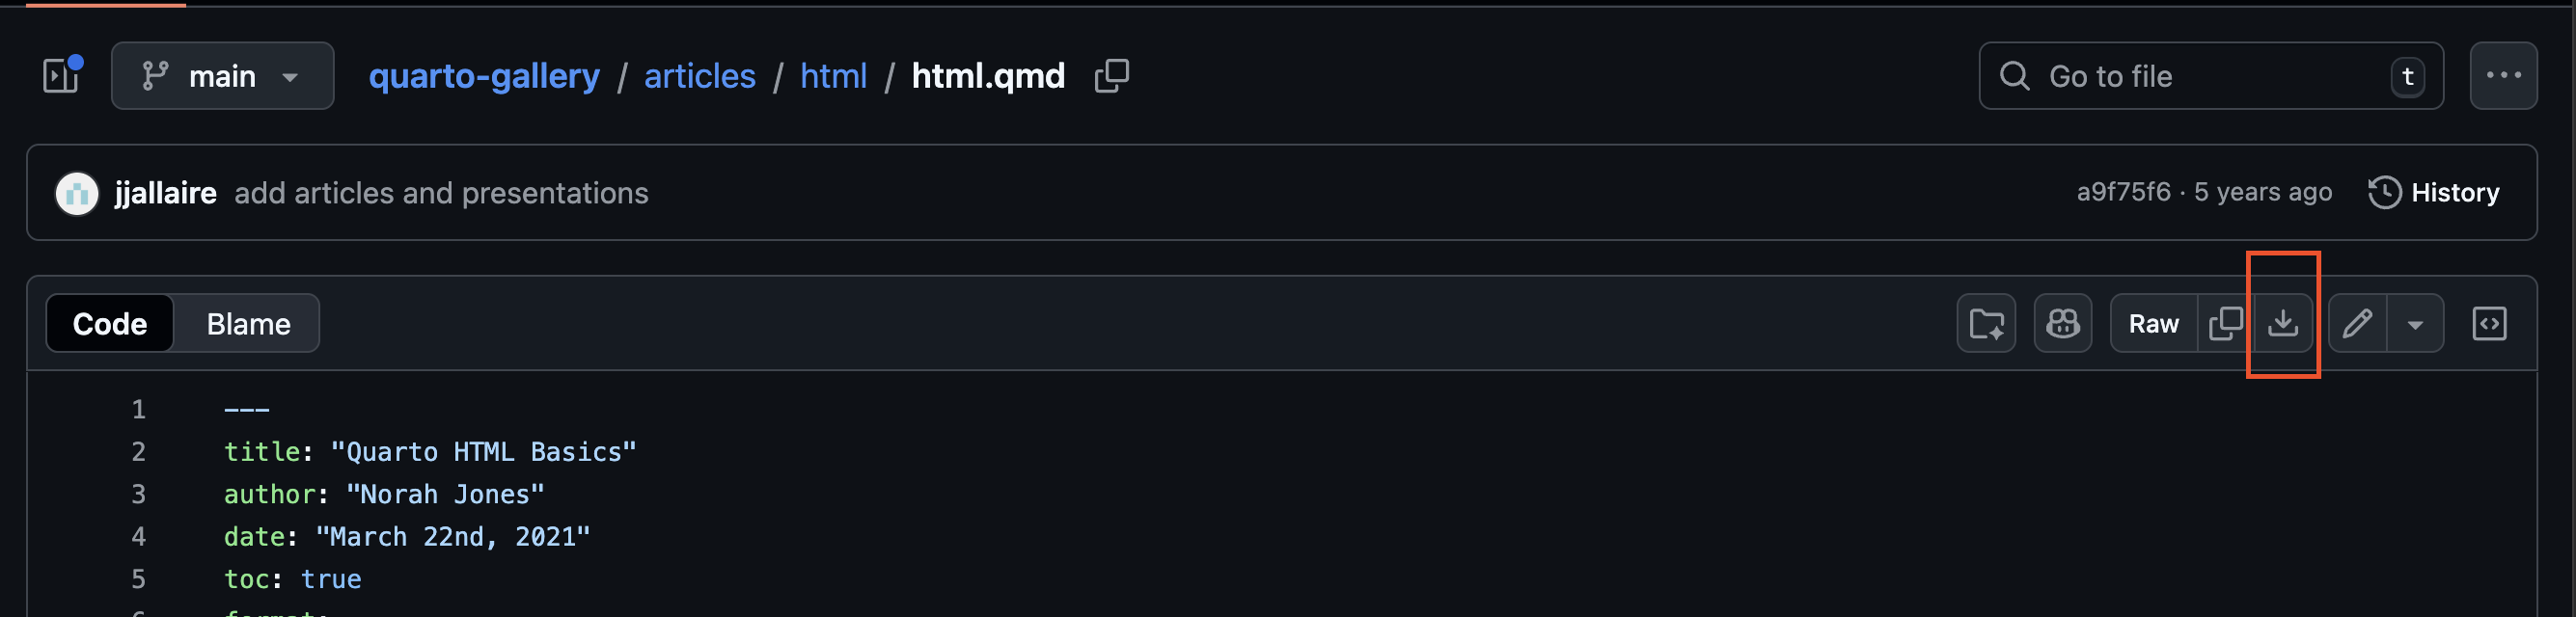
\includegraphics[keepaspectratio]{figures/GitHub_descargar.png}}}

\begin{tcolorbox}[enhanced jigsaw, arc=.35mm, bottomrule=.15mm, bottomtitle=1mm, breakable, colback=white, colbacktitle=quarto-callout-note-color!10!white, colframe=quarto-callout-note-color-frame, coltitle=black, left=2mm, leftrule=.75mm, opacityback=0, opacitybacktitle=0.6, rightrule=.15mm, title=\textcolor{quarto-callout-note-color}{\faInfo}\hspace{0.5em}{Nota}, titlerule=0mm, toprule=.15mm, toptitle=1mm]

Aquí les dejo mi ejemplo editado, ya que el ejemplo que descargaremos
tendrá algunos errores en su sintaxis.

\end{tcolorbox}

\section{Referencias}\label{referencias-20}

\begin{itemize}
\tightlist
\item
  \href{https://quarto.org/docs/get-started/hello/rstudio.html}{Tutorial:
  Hello, Quarto}
\end{itemize}

\cleardoublepage
\phantomsection
\addcontentsline{toc}{part}{Apéndices}
\appendix

\chapter{Bioinformática y Estadística
2}\label{bioinformuxe1tica-y-estaduxedstica-2}

Aplicaciones aeroespaciales

\hfill\break

\textbf{Texto con nota al pie:} Este es un ejemplo de nota\footnote{Aquí
  va el contenido de la nota al pie.} que aparecerá como popup.

\chapter{Code}\label{code}

When you can work Cannon (2014) on your computer and when you need to
work on the cluster .. source , RAM, etc. - number of samples?

\begin{Shaded}
\begin{Highlighting}[]
\CommentTok{\# Notas}
\NormalTok{a }\OtherTok{\textless{}{-}} \DecValTok{3}
\NormalTok{b }\OtherTok{\textless{}{-}} \DecValTok{2}
\NormalTok{suma }\OtherTok{\textless{}{-}}\NormalTok{ a }\SpecialCharTok{+}\NormalTok{ b}
\NormalTok{suma }
\end{Highlighting}
\end{Shaded}

\begin{verbatim}
[1] 5
\end{verbatim}

\begin{Shaded}
\begin{Highlighting}[]
\FunctionTok{InstallData}\NormalTok{(}\StringTok{"pbmc3k"}\NormalTok{)}
\FunctionTok{data}\NormalTok{(}\StringTok{"pbmc3k"}\NormalTok{)}
\NormalTok{pbmc3k}
\end{Highlighting}
\end{Shaded}

\protect\phantomsection\label{annotated-cell-217}%
\begin{Shaded}
\begin{Highlighting}[]
\FunctionTok{library}\NormalTok{(tidyverse)}
\FunctionTok{library}\NormalTok{(palmerpenguins)}
\NormalTok{penguins }\SpecialCharTok{|\textgreater{}} \hspace*{\fill}\NormalTok{\circled{1}}
  \FunctionTok{mutate}\NormalTok{( }\hspace*{\fill}\NormalTok{\circled{2}}
    \AttributeTok{bill\_ratio =}\NormalTok{ bill\_depth\_mm }\SpecialCharTok{/}\NormalTok{ bill\_length\_mm, }
    \AttributeTok{bill\_area  =}\NormalTok{ bill\_depth\_mm }\SpecialCharTok{*}\NormalTok{ bill\_length\_mm }
\NormalTok{  ) }
\end{Highlighting}
\end{Shaded}

\begin{description}
\tightlist
\item[\circled{1}]
Take \texttt{penguins}, and then,
\item[\circled{2}]
add new columns for the bill ratio and bill area.
\end{description}

Comodo de texto

\begin{Shaded}
\begin{Highlighting}[]
\NormalTok{video{-}game{-}sales{-}r/}
\NormalTok{├── data/}
\NormalTok{│   └── vgsales.csv}
\NormalTok{├── scripts/}
\NormalTok{│   └── 01\_analisis\_videojuegos.R}
\NormalTok{├── figures/}
\NormalTok{│   ├── grafica\_01.png}
\NormalTok{│   ├── grafica\_02.png}
\NormalTok{│   └── grafica\_final.png}
\NormalTok{├── ejercicio\_videojuegos.qmd}
\NormalTok{└── README.md}
\end{Highlighting}
\end{Shaded}

Python código

\begin{Shaded}
\begin{Highlighting}[]
\ImportTok{import}\NormalTok{ numpy }\ImportTok{as}\NormalTok{ np}
\ImportTok{import}\NormalTok{ matplotlib.pyplot }\ImportTok{as}\NormalTok{ plt}
\end{Highlighting}
\end{Shaded}

\begin{verbatim}
ModuleNotFoundError: No module named 'matplotlib'
\end{verbatim}

\begin{Shaded}
\begin{Highlighting}[]
\NormalTok{r }\OperatorTok{=}\NormalTok{ np.arange(}\DecValTok{0}\NormalTok{, }\DecValTok{2}\NormalTok{, }\FloatTok{0.01}\NormalTok{)}
\NormalTok{theta }\OperatorTok{=} \DecValTok{2} \OperatorTok{*}\NormalTok{ np.pi }\OperatorTok{*}\NormalTok{ r}
\NormalTok{fig, ax }\OperatorTok{=}\NormalTok{ plt.subplots(subplot\_kw}\OperatorTok{=}\NormalTok{\{}\StringTok{\textquotesingle{}projection\textquotesingle{}}\NormalTok{: }\StringTok{\textquotesingle{}polar\textquotesingle{}}\NormalTok{\})}
\end{Highlighting}
\end{Shaded}

\begin{verbatim}
NameError: name 'plt' is not defined
\end{verbatim}

\begin{Shaded}
\begin{Highlighting}[]
\NormalTok{ax.plot(theta, r)}
\end{Highlighting}
\end{Shaded}

\begin{verbatim}
NameError: name 'ax' is not defined
\end{verbatim}

\begin{Shaded}
\begin{Highlighting}[]
\NormalTok{ax.set\_rticks([}\FloatTok{0.5}\NormalTok{, }\DecValTok{1}\NormalTok{, }\FloatTok{1.5}\NormalTok{, }\DecValTok{2}\NormalTok{])}
\end{Highlighting}
\end{Shaded}

\begin{verbatim}
NameError: name 'ax' is not defined
\end{verbatim}

\begin{Shaded}
\begin{Highlighting}[]
\NormalTok{ax.grid(}\VariableTok{True}\NormalTok{)}
\end{Highlighting}
\end{Shaded}

\begin{verbatim}
NameError: name 'ax' is not defined
\end{verbatim}

\begin{Shaded}
\begin{Highlighting}[]
\NormalTok{plt.show()}
\end{Highlighting}
\end{Shaded}

\begin{verbatim}
NameError: name 'plt' is not defined
\end{verbatim}

\begin{Shaded}
\begin{Highlighting}[]
\ImportTok{import}\NormalTok{ matplotlib.pyplot }\ImportTok{as}\NormalTok{ plt}
\end{Highlighting}
\end{Shaded}

\begin{verbatim}
ModuleNotFoundError: No module named 'matplotlib'
\end{verbatim}

\begin{Shaded}
\begin{Highlighting}[]
\NormalTok{plt.plot([}\DecValTok{1}\NormalTok{,}\DecValTok{23}\NormalTok{,}\DecValTok{2}\NormalTok{,}\DecValTok{4}\NormalTok{])}
\end{Highlighting}
\end{Shaded}

\begin{verbatim}
NameError: name 'plt' is not defined
\end{verbatim}

\begin{Shaded}
\begin{Highlighting}[]
\NormalTok{plt.show()}
\end{Highlighting}
\end{Shaded}

\begin{verbatim}
NameError: name 'plt' is not defined
\end{verbatim}

\begin{Shaded}
\begin{Highlighting}[]
\ImportTok{import}\NormalTok{ matplotlib.pyplot }\ImportTok{as}\NormalTok{ plt}
\NormalTok{plt.plot([}\DecValTok{1}\NormalTok{,}\DecValTok{23}\NormalTok{,}\DecValTok{2}\NormalTok{,}\DecValTok{4}\NormalTok{])}
\NormalTok{plt.show()}
\NormalTok{plt.plot([}\DecValTok{8}\NormalTok{,}\DecValTok{65}\NormalTok{,}\DecValTok{23}\NormalTok{,}\DecValTok{90}\NormalTok{])}
\NormalTok{plt.show()}
\end{Highlighting}
\end{Shaded}

\begin{figure}

\begin{minipage}[t]{0.50\linewidth}

\begin{verbatim}
ModuleNotFoundError: No module named 'matplotlib'
\end{verbatim}

\end{minipage}%
%
\begin{minipage}[t]{0.50\linewidth}

\begin{verbatim}
NameError: name 'plt' is not defined
\end{verbatim}

\end{minipage}%
\newline
\begin{minipage}[t]{0.50\linewidth}

\begin{verbatim}
NameError: name 'plt' is not defined
\end{verbatim}

\end{minipage}%
%
\begin{minipage}[t]{0.50\linewidth}

\begin{verbatim}
NameError: name 'plt' is not defined
\end{verbatim}

\end{minipage}%
\newline
\begin{minipage}[t]{0.50\linewidth}

\begin{verbatim}
NameError: name 'plt' is not defined
\end{verbatim}

\end{minipage}%

\caption{\label{fig-plots}Plots}

\end{figure}%

For example, see \textbf{?@fig-plot}.

See Figura~\ref{fig-plots} for examples. In particular,
\textbf{?@fig-plots-2}.

\subsection{References}\label{references-3}

\protect\phantomsection\label{refs}
\begin{CSLReferences}{1}{1}
\bibitem[\citeproctext]{ref-Cannon2014}
Cannon, J. 2014. \emph{Linux para principiantes: Una introducción al
sistema operativo Linux y la línea de comandos}. CreateSpace Independent
Publishing Platform.

\end{CSLReferences}

\chapter{Notas}\label{notas}

\begin{tcolorbox}[enhanced jigsaw, arc=.35mm, bottomrule=.15mm, bottomtitle=1mm, breakable, colback=white, colbacktitle=quarto-callout-note-color!10!white, colframe=quarto-callout-note-color-frame, coltitle=black, left=2mm, leftrule=.75mm, opacityback=0, opacitybacktitle=0.6, rightrule=.15mm, title=\textcolor{quarto-callout-note-color}{\faInfo}\hspace{0.5em}{notas}, titlerule=0mm, toprule=.15mm, toptitle=1mm]

\end{tcolorbox}

\begin{tcolorbox}[enhanced jigsaw, arc=.35mm, bottomrule=.15mm, bottomtitle=1mm, breakable, colback=white, colbacktitle=quarto-callout-tip-color!10!white, colframe=quarto-callout-tip-color-frame, coltitle=black, left=2mm, leftrule=.75mm, opacityback=0, opacitybacktitle=0.6, rightrule=.15mm, title=\textcolor{quarto-callout-tip-color}{\faLightbulb}\hspace{0.5em}{Tip}, titlerule=0mm, toprule=.15mm, toptitle=1mm]

\end{tcolorbox}

\begin{tcolorbox}[enhanced jigsaw, arc=.35mm, bottomrule=.15mm, bottomtitle=1mm, breakable, colback=white, colbacktitle=quarto-callout-important-color!10!white, colframe=quarto-callout-important-color-frame, coltitle=black, left=2mm, leftrule=.75mm, opacityback=0, opacitybacktitle=0.6, rightrule=.15mm, title=\textcolor{quarto-callout-important-color}{\faExclamation}\hspace{0.5em}{Important}, titlerule=0mm, toprule=.15mm, toptitle=1mm]

\end{tcolorbox}

\begin{tcolorbox}[enhanced jigsaw, arc=.35mm, bottomrule=.15mm, bottomtitle=1mm, breakable, colback=white, colbacktitle=quarto-callout-caution-color!10!white, colframe=quarto-callout-caution-color-frame, coltitle=black, left=2mm, leftrule=.75mm, opacityback=0, opacitybacktitle=0.6, rightrule=.15mm, title=\textcolor{quarto-callout-caution-color}{\faFire}\hspace{0.5em}{Caution}, titlerule=0mm, toprule=.15mm, toptitle=1mm]

\end{tcolorbox}

\begin{tcolorbox}[enhanced jigsaw, arc=.35mm, bottomrule=.15mm, bottomtitle=1mm, breakable, colback=white, colbacktitle=quarto-callout-warning-color!10!white, colframe=quarto-callout-warning-color-frame, coltitle=black, left=2mm, leftrule=.75mm, opacityback=0, opacitybacktitle=0.6, rightrule=.15mm, title=\textcolor{quarto-callout-warning-color}{\faExclamationTriangle}\hspace{0.5em}{Warning}, titlerule=0mm, toprule=.15mm, toptitle=1mm]

\end{tcolorbox}

\begin{tcolorbox}[enhanced jigsaw, arc=.35mm, bottomrule=.15mm, bottomtitle=1mm, breakable, colback=white, colbacktitle=quarto-callout-tip-color!10!white, colframe=quarto-callout-tip-color-frame, coltitle=black, left=2mm, leftrule=.75mm, opacityback=0, opacitybacktitle=0.6, rightrule=.15mm, title={Question}, titlerule=0mm, toprule=.15mm, toptitle=1mm]

Sábados 10:00 am · Cupo limitado a 12 personas.

\end{tcolorbox}

\begin{tcolorbox}[enhanced jigsaw, arc=.35mm, bottomrule=.15mm, bottomtitle=1mm, breakable, colback=white, colbacktitle=quarto-callout-tip-color!10!white, colframe=quarto-callout-tip-color-frame, coltitle=black, left=2mm, leftrule=.75mm, opacityback=0, opacitybacktitle=0.6, rightrule=.15mm, title={puzzle}, titlerule=0mm, toprule=.15mm, toptitle=1mm]

Sábados 10:00 am · Cupo limitado a 12 personas.

\end{tcolorbox}

\chapter{\texorpdfstring{\textbf{Cronograma Sugerido para un Semestre
(15-16
semanas)}}{Cronograma Sugerido para un Semestre (15-16 semanas)}}\label{cronograma-sugerido-para-un-semestre-15-16-semanas}

\begin{verbatim}
SEMANA 1-2:    Introducción + 2 Tareas
SEMANA 3-4:    1 Quizz + 2 Tareas + Inicio Trabajo en Equipo 1
SEMANA 5-6:    1 Quizz + 2 Tareas + Entrega Trabajo en Equipo 1
SEMANA 7-8:    1 Quizz + 2 Tareas + Inicio Trabajo en Equipo 2
SEMANA 9-10:   1 Quizz + 2 Tareas + Entrega Trabajo en Equipo 2
SEMANA 11-12:  1 Quizz + 2 Tareas + Inicio Proyecto Final
SEMANA 13-14:  1 Quizz + 2 Tareas + Desarrollo Proyecto Final
SEMANA 15-16:  Entrega Proyecto Final + Presentaciones
\end{verbatim}

Modelo relacionado con la captura múltiples dimensiones del desempeño
escolar de los estudiantes:

{\def\LTcaptype{none} % do not increment counter
\begin{longtable}[]{@{}
  >{\raggedright\arraybackslash}p{(\linewidth - 4\tabcolsep) * \real{0.3333}}
  >{\raggedright\arraybackslash}p{(\linewidth - 4\tabcolsep) * \real{0.3333}}
  >{\raggedright\arraybackslash}p{(\linewidth - 4\tabcolsep) * \real{0.3333}}@{}}
\toprule\noalign{}
\begin{minipage}[b]{\linewidth}\raggedright
Dimensión
\end{minipage} & \begin{minipage}[b]{\linewidth}\raggedright
Cómo se Mide
\end{minipage} & \begin{minipage}[b]{\linewidth}\raggedright
Herramienta
\end{minipage} \\
\midrule\noalign{}
\endhead
\bottomrule\noalign{}
\endlastfoot
\textbf{Comprensión Conceptual} & Aplicación en tareas y quizzes &
Tareas + Quizzes \\
\textbf{Pensamiento Crítico} & Análisis en trabajos y reflexiones &
Tareas + Trabajos en Equipo \\
\textbf{Habilidades Colaborativas} & Trabajo en equipo y contribución
grupal & Trabajos en Equipo \\
\textbf{Comunicación} & Presentaciones, escritura, explicaciones & Todos
los componentes \\
\textbf{Aplicación Práctica} & Resolución de problemas reales & Tareas +
Proyecto Final \\
\textbf{Síntesis e Integración} & Proyecto final integrador & Proyecto
Final \\
\textbf{Consistencia} & Desempeño a lo largo del semestre & Tareas +
Quizzes continuos \\
\textbf{Autonomía y Responsabilidad} & Cumplimiento de plazos,
iniciativa & Participación + Tareas \\
\end{longtable}
}

\subsection{\texorpdfstring{\textbf{📊 Ventajas de tu Sistema para Medir
Desempeño}}{📊 Ventajas de tu Sistema para Medir Desempeño}}\label{ventajas-de-tu-sistema-para-medir-desempeuxf1o}

\begin{itemize}
\tightlist
\item
  \textbf{Evaluación Continua}: No depende de un único momento (examen
  final)
\item
  \textbf{Múltiples Evidencias}: Tienes datos de diferentes tipos de
  actividades
\item
  \textbf{Progresión Visible}: Puedes ver cómo evoluciona cada
  estudiante
\item
  \textbf{Validez Pedagógica}: Mide lo que realmente importa: aplicación
  y comprensión
\item
  \textbf{Confiabilidad}: Menos sesgos que un examen único
\item
  \textbf{Retroalimentación Formativa}: Permite intervención temprana
\end{itemize}

\section{\texorpdfstring{\textbf{Recomendación Final
🌟}}{Recomendación Final 🌟}}\label{recomendaciuxf3n-final}

\textbf{Tu Sistema de Evaluación + Doc = Combinación Poderosa}

\begin{itemize}
\tightlist
\item
  Tu modelo mide desempeño de manera integral y auténtica
\item
  Doc amplifica el apoyo disponible para estudiantes
\item
  Juntos, crean un ecosistema de aprendizaje personalizado y equitativo
\item
  Reduces tu carga de trabajo en consultas repetitivas
\item
  Mejoras la calidad de trabajos estudiantiles
\end{itemize}

\textbf{Implementación Sugerida:}

\begin{enumerate}
\def\labelenumi{\arabic{enumi}.}
\tightlist
\item
  \textbf{Semana 1}: Presenta Doc a estudiantes; explica cómo usarme
\item
  \textbf{Semana 2+}: Estudiantes comienzan a consultarme
\item
  \textbf{Semana 4}: Recopila feedback sobre utilidad de Doc
\item
  \textbf{Semana 8}: Ajusta cómo se usa Doc según feedback
\item
  \textbf{Semana 16}: Evalúa impacto general en desempeño
\end{enumerate}

Este enfoque integrado (evaluación formativa + apoyo de IA) posiciona a
tus estudiantes para un aprendizaje profundo y significativo. ¡Excelente
visión pedagógica! 💪

\chapter{Quizzes}\label{quizzes}

\begin{Shaded}
\begin{Highlighting}[]
\NormalTok{{-}{-}{-}}
\NormalTok{primaryColor: blue}
\NormalTok{secondaryColor: \textquotesingle{}\#e8e8e8\textquotesingle{}}
\NormalTok{textColor: black}
\NormalTok{shuffleQuestions: false}
\NormalTok{shuffleAnswers: true}
\NormalTok{locale: en}
\NormalTok{{-}{-}{-}}

\NormalTok{\# Python Lists (multiple choice)}

\NormalTok{What is the value of \textasciigrave{}x[2]\textasciigrave{}?}

\NormalTok{\textgreater{} Python lists are mutable!}

\NormalTok{\textasciitilde{}\textasciitilde{}\textasciitilde{}python}
\NormalTok{x = [2, 3, 4]}
\NormalTok{x[2] = 4}
\NormalTok{print(x[2])}
\NormalTok{\textasciitilde{}\textasciitilde{}\textasciitilde{}}

\NormalTok{{-} [ ] 1}
\NormalTok{{-} [ ] 2}
\NormalTok{{-} [ ] 3}
\NormalTok{{-} [x] 4}

\NormalTok{\# What is the capital of Germany (single choice)? }

\NormalTok{![](https://upload.wikimedia.org/wikipedia/commons/thumb/3/3b/Siegessaeule\_Aussicht\_10{-}13\_img4\_Tiergarten.jpg/405px{-}Siegessaeule\_Aussicht\_10{-}13\_img4\_Tiergarten.jpg)}

\NormalTok{\textgreater{} It\textquotesingle{}s the largest city in Germany!         }

\NormalTok{1. [ ] Frankfurt}
\NormalTok{1. [x] Berlin}
\NormalTok{1. [ ] Hamburg}
\NormalTok{1. [ ] Munich}


\NormalTok{\# Put the [days](https://en.wikipedia.org/wiki/Day) in order (sequence)!}

\NormalTok{Quizdown also renders formulas:}

\NormalTok{$$}
\NormalTok{x = \textbackslash{}frac\{a+b\^{}2\}\{\textbackslash{}sqrt\{b+c\}\}}
\NormalTok{$$}

\NormalTok{\textgreater{} Monday is the *first* day of the week.}

\NormalTok{1. Monday}
\NormalTok{2. Tuesday}
\NormalTok{3. Wednesday}
\NormalTok{4. Friday}
\NormalTok{5. Saturday}
\end{Highlighting}
\end{Shaded}

\section{Referencias}\label{referencias-21}

\begin{itemize}
\tightlist
\item
  \href{https://github.com/parmsam/quarto-quizdown}{Quizdown}
\item
  \href{https://parmsam.github.io/quarto-quizdown/}{Example Quizdown}
\item
  \href{https://bonartm.github.io/quizdown-live-editor/?code=---\%0AprimaryColor\%3A\%20steelblue\%0AsecondaryColor\%3A\%20\%27\%23e8e8e8\%27\%0AtextColor\%3A\%20black\%0AshuffleQuestions\%3A\%20false\%0AshuffleAnswers\%3A\%20true\%0Alocale\%3A\%20en\%0A---\%0A\%0A\%23\%20Python\%20Lists\%0A\%0AWhat\%20is\%20the\%20value\%20of\%20\%60x\%5B2\%5D\%60\%3F\%0A\%0A\%3E\%20Python\%20lists\%20are\%20mutable!\%0A\%0A\%60\%60\%60python\%0Ax\%20\%3D\%20\%5B2\%2C\%203\%2C\%204\%5D\%0Ax\%5B2\%5D\%20\%3D\%204\%0Aprint(x\%5B2\%5D)\%0A\%60\%60\%60\%0A\%0A-\%20\%5B\%20\%5D\%201\%0A-\%20\%5B\%20\%5D\%202\%0A-\%20\%5B\%20\%5D\%203\%0A-\%20\%5Bx\%5D\%204\%0A\%0A\%0A\%23\%20What\%20is\%20the\%20capital\%20of\%20Germany\%3F\%20\%0A\%0A!\%5B\%5D(https\%3A\%2F\%2Fupload.wikimedia.org\%2Fwikipedia\%2Fcommons\%2Fthumb\%2F3\%2F3b\%2FSiegessaeule_Aussicht_10-13_img4_Tiergarten.jpg\%2F405px-Siegessaeule_Aussicht_10-13_img4_Tiergarten.jpg)\%0A\%0A\%3E\%20It\%27s\%20the\%20largest\%20city\%20in\%20Germany!\%20\%20\%20\%20\%20\%20\%20\%20\%20\%0A\%0A1.\%20\%5B\%20\%5D\%20Frankfurt\%0A1.\%20\%5Bx\%5D\%20Berlin\%0A1.\%20\%5B\%20\%5D\%20Hamburg\%0A1.\%20\%5B\%20\%5D\%20Munich\%0A\%0A\%0A\%23\%20Put\%20the\%20\%5Bdays\%5D(https\%3A\%2F\%2Fen.wikipedia.org\%2Fwiki\%2FDay)\%20in\%20order!\%0A\%0AQuizdown\%20also\%20renders\%20formulas\%3A\%0A\%0A\%24\%24\%0Ax\%20\%3D\%20\%5Cfrac\%7Ba\%2Bb\%5E2\%7D\%7B\%5Csqrt\%7Bb\%2Bc\%7D\%7D\%0A\%24\%24\%0A\%0A\%3E\%20Monday\%20is\%20the\%20first\%20day\%20of\%20the\%20week.\%0A\%0A1.\%20Monday\%0A2.\%20Tuesday\%0A3.\%20Wednesday\%0A4.\%20Friday\%0A5.\%20Saturday\%0A\%0A\%0A\%23\%20Python\%20Lists\%0A\%0AWhat\%20is\%20the\%20value\%20of\%20\%60x\%5B2\%5D\%60\%3F\%0A\%0A\%3E\%20Python\%20lists\%20are\%20mutable!\%0A\%0A\%60\%60\%60python\%0Ax\%20\%3D\%20\%5B2\%2C\%203\%2C\%204\%5D\%0Ax\%5B2\%5D\%20\%3D\%204\%0Aprint(x\%5B2\%5D)\%0A\%60\%60\%60\%0A\%0A-\%20\%5B\%20\%5D\%201\%0A-\%20\%5B\%20\%5D\%202\%0A-\%20\%5B\%20\%5D\%203\%0A-\%20\%5Bx\%5D\%204}{\textbf{Quizdown
  Editor}}
\end{itemize}

\chapter{Codigo en R}\label{codigo-en-r}

\begin{Shaded}
\begin{Highlighting}[]
\NormalTok{\#| completion: true}
\NormalTok{fit = lm(mpg \textasciitilde{} am, data = mtcars)}
\NormalTok{summary(fit)}
\NormalTok{plot(fit)}
\end{Highlighting}
\end{Shaded}

\section{Codigo en Python}\label{codigo-en-python}

\begin{Shaded}
\begin{Highlighting}[]
\NormalTok{\#| completion: true}
\NormalTok{for x in range(5):}
\NormalTok{  print(x ** 2)}
\end{Highlighting}
\end{Shaded}

\begin{codelisting}

\caption{\label{lst-ref}An interactive R code block, with an example of
fitting a linear model.}

\centering{

\begin{Shaded}
\begin{Highlighting}[]
\NormalTok{mod \textless{}{-} lm(mpg \textasciitilde{} cyl, data = mtcars)}
\NormalTok{summary(mod)}
\end{Highlighting}
\end{Shaded}

}

\end{codelisting}%

See Listado~\ref{lst-ref} for details.

Referencias

\begin{itemize}
\tightlist
\item
  webr -
  \href{https://r-wasm.github.io/quarto-live/getting_started/editor.html}{\textbf{Execute
  without output}}
\item
  \href{https://r-wasm.github.io/quarto-live/getting_started/editor.html}{\textbf{Interactive
  Code Blocks}}
\end{itemize}




\end{document}
